%\documentclass[11pt, paper=a4]{scrartcl}
\documentclass[11pt, paper=a4]{scrbook}
\usepackage{scrhack}
\usepackage[T1]{fontenc}
\usepackage[utf8]{inputenc}
\usepackage{graphicx}
\usepackage{amsmath,amsfonts,amssymb, amsthm}
\usepackage{bm}
\usepackage{graphicx}
\usepackage{color}
\usepackage{rotating}
\usepackage{cite}
\usepackage{textcomp}
\usepackage{lmodern}
\usepackage{color}
%\usepackage{chngcntr}
% makes Fig number in the form Fig. <Section-Nr>.number with number being reset after every section (i.e. new blog entry)
%\counterwithin{figure}{section}
\counterwithin{equation}{section}
\usepackage{hyperref}
\usepackage{makeidx}
\usepackage{float}
\usepackage{caption}
\usepackage{subcaption}
\usepackage{longtable}
\usepackage{tabu}
\usepackage{fancyvrb}
\makeindex

%\usepackage{pstricks}


\setlength{\parindent}{0pt}

\usepackage{tikz}
% \usepackage{tkz-graph}

\usepackage{todonotes}


\newcommand{\abf}{\mathbf{a}}
\newcommand{\bbf}{\mathbf{b}}
\newcommand{\cbf}{\mathbf{c}}
\newcommand{\dbf}{\mathbf{d}}
\newcommand{\ebf}{\mathbf{e}}
\newcommand{\fbf}{\mathbf{f}}
\newcommand{\gbf}{\mathbf{g}}
\newcommand{\hbf}{\mathbf{h}}
\newcommand{\ibf}{\mathbf{i}}
\newcommand{\jbf}{\mathbf{j}}
\newcommand{\kbf}{\mathbf{k}}
\newcommand{\lbf}{\mathbf{l}}
\newcommand{\mbf}{\mathbf{m}}
\newcommand{\nbf}{\mathbf{n}}
\newcommand{\obf}{\mathbf{o}}
\newcommand{\pbf}{\mathbf{p}}
\newcommand{\qbf}{\mathbf{q}}
\newcommand{\rbf}{\mathbf{r}}
\newcommand{\sbf}{\mathbf{s}}
\newcommand{\tbf}{\mathbf{t}}
\newcommand{\ubf}{\mathbf{u}}
\newcommand{\vbf}{\mathbf{v}}
\newcommand{\wbf}{\mathbf{w}}
\newcommand{\xbf}{\mathbf{x}}
\newcommand{\ybf}{\mathbf{y}}
\newcommand{\zbf}{\mathbf{z}}



\newcommand{\Abf}{\mathbf{A}}
\newcommand{\Bbf}{\mathbf{B}}
\newcommand{\Cbf}{\mathbf{C}}
\newcommand{\Dbf}{\mathbf{D}}
\newcommand{\Ebf}{\mathbf{E}}
\newcommand{\Fbf}{\mathbf{F}}
\newcommand{\Gbf}{\mathbf{G}}
\newcommand{\Hbf}{\mathbf{H}}
\newcommand{\Ibf}{\mathbf{I}}
\newcommand{\Kbf}{\mathbf{K}}
\newcommand{\Lbf}{\mathbf{L}}
\newcommand{\Mbf}{\mathbf{M}}
\newcommand{\Nbf}{\mathbf{N}}
\newcommand{\Obf}{\mathbf{O}}
\newcommand{\Pbf}{\mathbf{P}}
\newcommand{\Qbf}{\mathbf{Q}}
\newcommand{\Rbf}{\mathbf{R}}
\newcommand{\Sbf}{\mathbf{S}}
\newcommand{\Tbf}{\mathbf{T}}
\newcommand{\Ubf}{\mathbf{U}}
\newcommand{\Vbf}{\mathbf{V}}
\newcommand{\Wbf}{\mathbf{W}}
\newcommand{\Xbf}{\mathbf{X}}
\newcommand{\Ybf}{\mathbf{Y}}
\newcommand{\Zbf}{\mathbf{Z}}

\newcommand{\zerobf}{\mathbf{0}}
\newcommand{\onebf}{\mathbf{1}}
\newcommand{\Sigmabf}{\mathbf{\Sigma}}

\newcommand{\Ac}{\mathcal{A}}
\newcommand{\Bc}{\mathcal{B}}
\newcommand{\Dc}{\mathcal{D}}
\newcommand{\Ec}{\mathcal{E}}
\newcommand{\Gc}{\mathcal{G}}
\newcommand{\Ic}{\mathcal{I}}
\newcommand{\Nc}{\mathcal{N}}
\newcommand{\CNc}{\mathcal{CN}}
\newcommand{\Oc}{\mathcal{O}}
\newcommand{\Qc}{\mathcal{Q}}
\newcommand{\Cc}{\mathcal{C}}
\newcommand{\Sc}{\mathcal{S}}
\newcommand{\Vc}{\mathcal{V}}
\newcommand{\Zc}{\mathcal{Z}}

\newcommand{\mB}{\mathbb{B}}
\newcommand{\mC}{\mathbb{C}}
\newcommand{\mE}{\mathbb{E}}
\newcommand{\mF}{\mathbb{F}}
\newcommand{\mQ}{\mathbb{Q}}
\newcommand{\mR}{\mathbb{R}}
\newcommand{\mZ}{\mathbb{Z}}

\newcommand{\erf}{\mathrm{erf}}
\newcommand{\erfc}{\mathrm{erfc}}
\newcommand{\Exp}{\mathrm{E}}


\newcommand{\be}{\begin{equation}}
\newcommand{\ee}{\end{equation}}

\newcommand{\bee}{\begin{equation*}}
\newcommand{\eee}{\end{equation*}}


\newcommand{\bea}{\begin{align*}}
\newcommand{\eea}{\end{align*}}



% a command to generate a new diary entry
% parameters: title, date, category
\newcommand{\DiaryEntry}[3]{
  %\pagebreak
  %\vspace*{3mm}
  \section{#1, #2}\index{#3!#1 - #2}
  \vspace*{-3mm}
  \textit{#2 #3}

  \noindent\rule{8cm}{0.5pt}
  \vspace{3mm}
  \label{#2:entry}
}

\newtheorem{definition}{Definition}[section]
\newtheorem{theorem}{Theorem}[section]
\newtheorem{problem}{Problem}[section]

\DeclareMathOperator{\lcm}{lcm}
\DeclareMathOperator{\atantwo}{atan2}


\begin{document}

\title{My Personal Journal}
\author{}
\date{}

\maketitle

\tableofcontents

\printindex

\chapter{Entries}

%\DiaryEntry{Least Squares}{2015-06-26}{Maths}


Derivation of the least-squares expression: Given the system matrix \(\mathbf{A}\) and the observation \(\mathbf{y}\), we seek the \(\mathbf{\hat{x}}\) so that the error \(\mathbf{r} = \mathbf{y} - \mathbf{A} \mathbf{x}\) is minimized.

%\pagebreak

\begin{figure}[htb!]
\centering
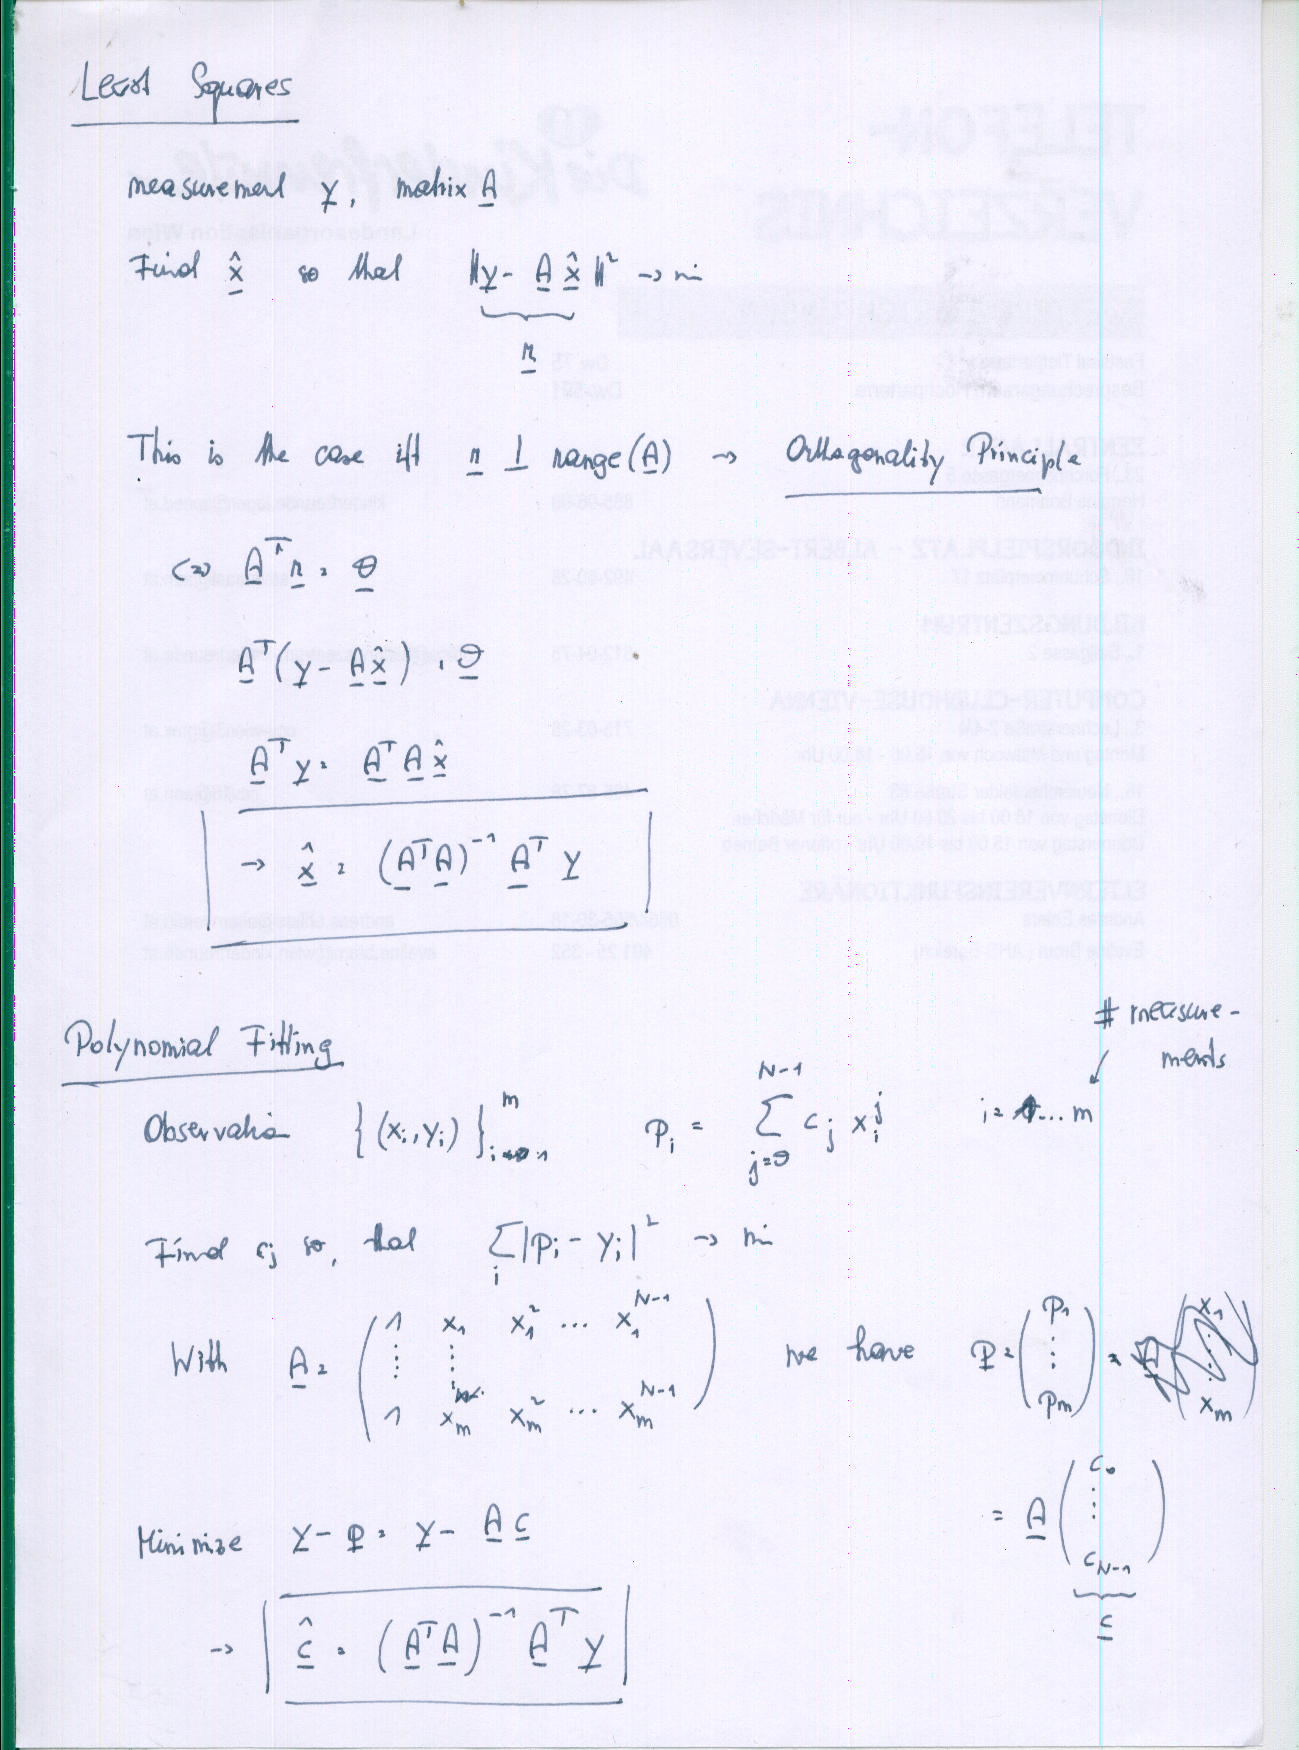
\includegraphics[scale=0.5]{images/least_squares.png}
\caption{Derivation}
\end{figure}

Seen another way, the result \(\mathbf{\hat{x}} = (\mathbf{A}^T \mathbf{A})^{-1} \mathbf{A}^T \mathbf{y}\) is the projection of \(\mathbf{y}\) onto the vector space defined by the columns of \(\mathbf{A}\).

\subsection{Least Squares Example (Julia)}

We consider \(\mathbb{R}^3\) and want to project onto the x-y plane; first we choose the matrix \(\mathbf{A} = [\mathbf{e_1} \mathbf{e_2}]\)

\begin{verbatim}
A=[1 0;0 1;0 0]
inv(A'*A)*A'

2x3 Array{Float64,2}:
1.0  0.0  0.0
0.0  1.0  0.0
\end{verbatim}

The least squares matrix considers only the first two components of any vector it is applied onto =\textgreater{} projection onto x-y plane.

Similarly, nothing (much) changes, if we choose different vectors \(\mathbf{u_1}, \mathbf{u_2}\) for \(\mathbf{A} = [\mathbf{u_1} \mathbf{u_2}]\), as long as they are part of the x-y plane:

\begin{verbatim}
A=[sqrt(2)/2 -sqrt(2)/2;sqrt(2)/2 sqrt(2)/2;0 0]

3x2 Array{Float64,2}:
0.707107  -0.707107
0.707107   0.707107
0.0        0.0     

inv(A'*A)*A'

2x3 Array{Float64,2}:
0.707107  0.707107  0.0
-0.707107  0.707107  0.0
\end{verbatim}

\subsection{Least Squares Polynomial Fitting Example (Julia)}

\subsubsection{No Noise}

We consider \(x_i={-2,-1.2,-0.4,0.4,1.2,2}\) and $y_i=x_i^3$. We least-squares fit three polynoms onto the point set \({x_i,y_i}\) with degree \(N=1\) (a straight line); \(N=3\) (a polynom of the same order as the ``model''), and \(N=6\); i.e. a polynomial with a higher order.

\begin{verbatim}
using Winston

N = 6
srand(1234)

x = linspace(-2,2,N)
y = x.^3

yobs = y

A1 = [x.^0 x.^1]
A3 = [x.^0 x.^1 x.^2 x.^3]
A5 = [x.^0 x.^1 x.^2 x.^3 x.^4 x.^5]


c_hat_1 = inv(A1'*A1)*A1'*yobs
c_hat_3 = inv(A3'*A3)*A3'*yobs
c_hat_5 = inv(A5'*A5)*A5'*yobs

plot(x,yobs,"-rx", x,A1*c_hat_1,"ob", x,A3*c_hat_3,"og", x,A5*c_hat_5,"oy")
savefig("ls_polyfit.pdf")
\end{verbatim}

The following plot shows the results for these different degrees. The observed data is shown in red with circles. The polynomial with $N=1$ (blue circles) gives a bad fit; both $N=3$ (green circles) and $N = 6$ (yellow pluses) yield a pefect match.

\begin{figure}[htb!]
\centering
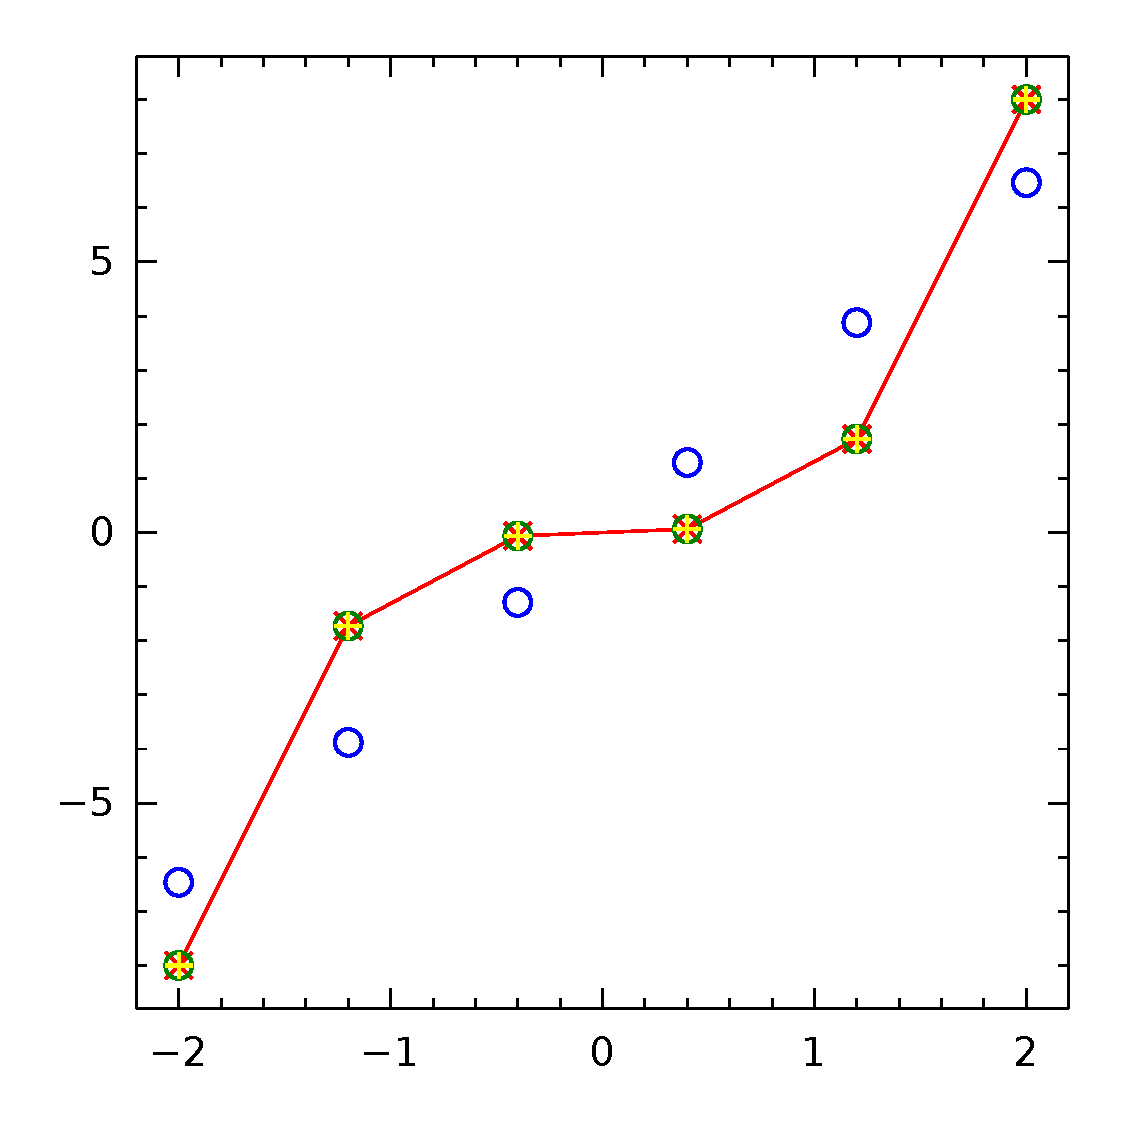
\includegraphics[scale=0.5]{images/ls_polyfit_no_noise.pdf}
\caption{Approximation of noise-free observation with polynomials of degree 1, degree 3, and degree 6, respectively.}
\end{figure}

The coefficient values are as follows

\begin{verbatim}
c_hat_3
4-element Array{Float64,1}:
 0.0       
 1.9984e-15
 0.0       
 1.0

c_hat_5
6-element Array{Float64,1}:
 0.0        
 4.59077e-14
 1.11022e-16
 1.0        
 0.0        
 2.89768e-14

\end{verbatim}

That is, they perfectly match the polynomial $x^3$.


\subsubsection{Measurement with Noise}

Things become different, when the observations are noisy; i.e. $y_i=x_i^3 + w_i$ with the $w_i$ some random Gaussian noise having variance $1$.

The plot below shows the results in this case. It can be seen that the polynomial $N=3$ is now an imperfect match while the polynomial with $N=6$ still has a perfect match: A polynomial of degree $6$ can perfectly match a sequence of $6$ datapoints.


\begin{figure}[htb!]
\centering
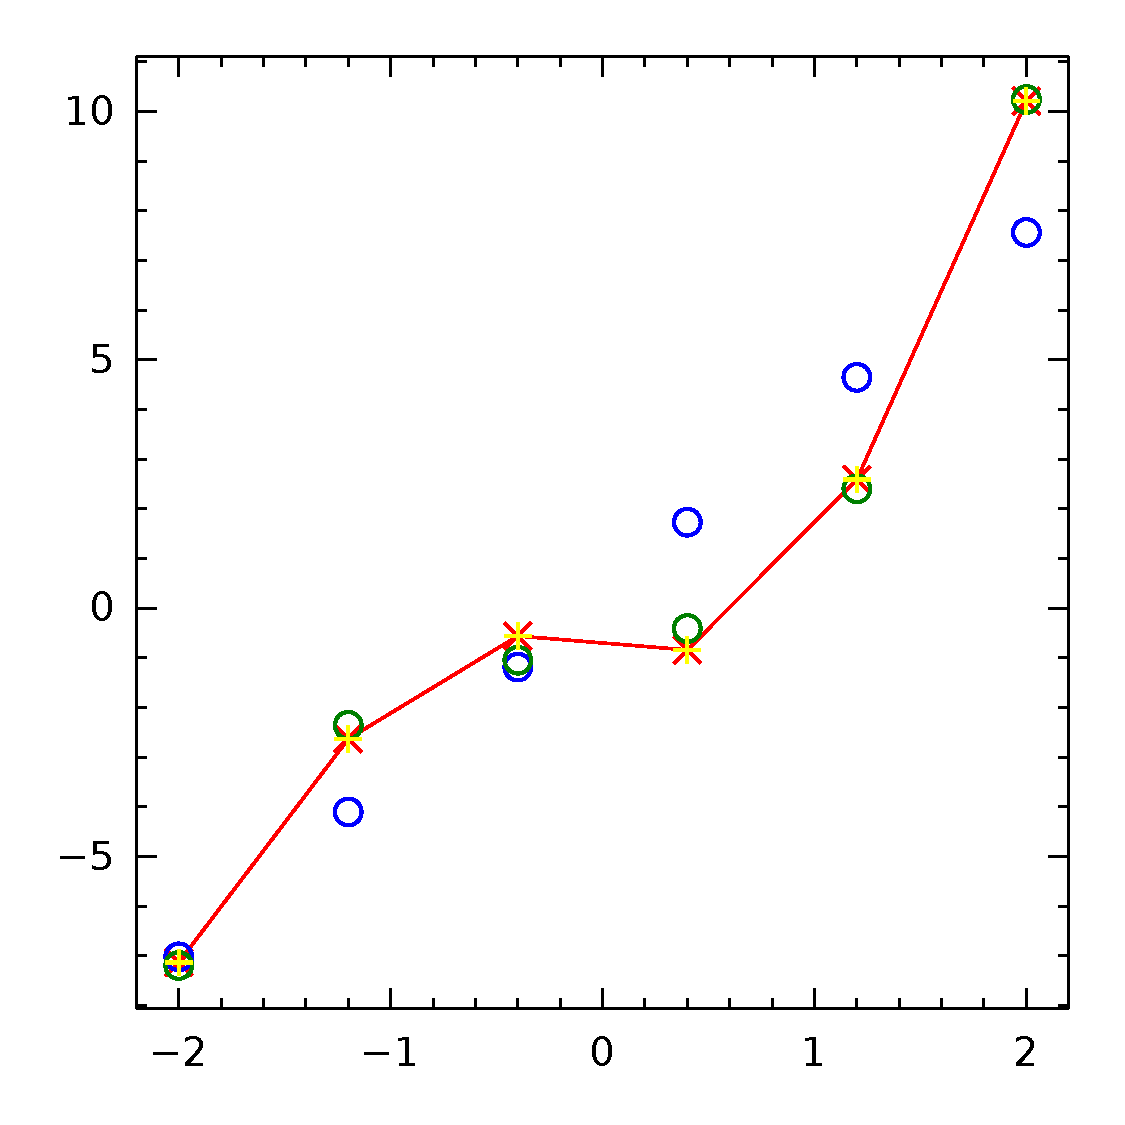
\includegraphics[scale=0.5]{images/ls_polyfit_with_noise.pdf}
\caption{Approximation of noise observation with polynomials of degree 1, degree 3, and degree 6, respectively.}
\end{figure}

%\DiaryEntry{Programming Languages}{2015-06-27}{Programming}

\subsection{Tasks}\label{tasks}

\begin{enumerate}
\def\labelenumi{\arabic{enumi}.}
\item
  Numerical stuff (lin. alg., (statistical)signal progessing,
  plotting\ldots{})
\item
  Scripting language for simple, day-to-day stuff
\item
  Gui development; i.e.~Qucs complexity level
\item
  something non-standard, supporting advanced concepts; e.g.~functional
  programming, macros, actors\ldots{}
\item
  something for web applications(?)
\end{enumerate}

\subsection{Languages}\label{languages}

\subsubsection{Julia}\label{julia}

Advantages: Modern, performant. Vector / matrix\ldots{} support ootb. A
language for scientific computing. Quite vibrant ecosystem but not as
complete as Python -\textgreater{} use PyCall.

\subsubsection{Python}\label{python}

Nice for everyday scripting, but numerical stuff (numpy) is awkward;
e.g.

\begin{verbatim}
self.current_x_hat = dot(A, x_hat)
self.current_Sigma = dot(A, dot(Sigma, A.T)) + Q
\end{verbatim}

Vectors are supported, but matrices are not really integrated into the
language. A general purpose language with support for scientific
computing (see Julia). Julia offers with PyCall a nice way to tap into
the Python scientific ecosystem.

\subsubsection{C\# / Mono + Winforms}\label{c-mono-winforms}

The ``classical'' way to go; cross-platform, lots of documentation
available (Windows World), sufficiently ``modern'' (more than Java).

\subsubsection{Scheme / Racket}\label{scheme-racket}

Seems to be sufficiently close to ``classical LISP books'' (SICP, The
little Schemer\ldots{}) to use it; nice IDE and nice library ecosystem.

\subsubsection{Ruby}\label{ruby}

Perfect for the few web apps I do (e.g.~in contrast to Django). In
addition, maybe it can replace Python as everyday scripting language.
Need to check ecosystem and compare with Python (main competitor).
Nicer/cleaner syntax/structure than Python in any case; e.g.

Python:

\begin{verbatim}
x = [1,4,3,6]
len(x)
but: x.sort() is a method which does in-place modification!
\end{verbatim}

Ruby

\begin{verbatim}
x = [1,4,3,6]
x.size
x.sort returns a sorted list; no in-place modification!
x.sort! sorts in-place
\end{verbatim}

\subsubsection{C++ / Qt}\label{c-qt}

Qt is a quite complete framework; so C++ with Qt is not ``really'' C++.
Nevertheless, too cumbersome and replaced by C\# / Mono with WinForms.

\subsubsection{Java / Swing}\label{java-swing}

Java is enterprise, but Swing is a bit old =\textgreater{} C\# / Mono +
WinForms is more modern.

\subsubsection{Scala}\label{scala}

Coming up as something new. Uses the JVM =\textgreater{} large
ecosystem. Sufficiently modern / functional / cool. Not overly hyped and
not so weird as e.g.~Haskell.

\subsubsection{Rust}\label{rust}

Nope - I don't think it introduces new concepts, but tries to be a
better (safer) C/C++. However, for all microcontroller/low-level system
stuff, there is C. No need for another Baustelle.

%\section{Interesting Stuff to Read}


\subsection{Papers}

\begin{itemize}

	\item \href{files/Ask HN_ What is the most mind blowing book you've ever read_ _ Hacker News.pdf}{Ask HN: What is the most mind blowing book you've ever read?}

	\item \href{files/Ask HN_ What books have made the biggest impact on your mental models_ _ Hacker News.pdf}{Ask HN: What books have made the biggest impact on your mental models?}

\end{itemize}
	
\subsubsection{Maths}

\begin{itemize}

	\item \href{http://math.stackexchange.com/questions/765198/some-users-are-mind-bogglingly-skilled-at-integration-how-did-they-get-there/1063528\#1063528}{Integration
	Skills}; Special Highlight: \href{http://faculty.swosu.edu/michael.dougherty/book/chapter07.pdf}{Advanced
	Integration Techniques}

	\item arXiv Articles:

	\begin{itemize}
		\item \href{http://arxiv.org/abs/1503.09060}{A Tutorial Introduction to
			the Lambda Calculus}
		\item \href{http://arxiv.org/abs/1503.00875}{Topologies and all that -- A
			Tutorial}
		\item \href{http://arxiv.org/abs/1506.00982}{Game Theory for Signal
			Processing in Networks}
		\item \href{http://arxiv.org/abs/0711.0189}{A Tutorial on Spectral
			Clustering}
	\end{itemize}

	\item \href{http://www.sigplan.org/Newsletters/CACM/Papers/}{SigPlan - CACM Papers}

	\item \href{https://pomax.github.io/bezierinfo/}{A Primer on Bezier Curves}

	\item \href{http://www.jamestanton.com/?category_name=puzzles}{Think Puzzles and Think Cool Math}

	\item \href{dice1.pdf}{A Collection of Dice Problems}

	\item \href{https://probabilityandstats.wordpress.com/}{A Blog on
	Probability and Statistics}

	\item  \href{http://www.galois-group.net/g/EN/theory.html}{The Evariste Galois Archive}

\end{itemize}

\subsubsection{Computer Science}

\begin{itemize}
	
	\item \href{files/Ask HN_ What are your favorite scholarly papers_ Why_ _ Hacker News.pdf}{Ask HN:What are your favorite scholarly papers? Why?}
	
	\item \href{https://github.com/papers-we-love/papers-we-love}{Papers we
		love}

	\item \href{files/Ask HN_ What is your favorite CS paper_ _ Hacker News.pdf}{Ask HN: What is your favorite CS paper?}

	\item \href{files/Ask HN_ What language-agnostic programming books should I read_ _ Hacker News.pdf}{Ask HN: What language-agnostic programming books should I read?}

	\item Monad Stuff

	\begin{itemize}
		\item
		\href{http://bartoszmilewski.com/2015/05/11/using-monads-in-c-to-solve-constraints-1-the-list-monad/}{Link1}
		\item
		\href{http://blog.jle.im/entry/unique-sample-drawing-searches-with-list-and-statet}{Link2}
		\item
		\href{http://www.berniepope.id.au/docs/scala_monads.pdf}{Link3}
		\item
		\href{http://james-iry.blogspot.co.at/2007/10/monads-are-elephants-part-3.html}{Link4}
	\end{itemize}

\end{itemize}

\subsection{Books}

\subsubsection{Maths}

\begin{itemize}

	\item \href{http://people.math.gatech.edu/~cain/textbooks/onlinebooks.html}{Online Mathematics Textbooks}

	\item \href{http://wstein.org/ent/}{Elementary Number Theory: Primes, Congruences, and Secrets}
	
	\item \href{http://aurellem.org/thoughts/html/sussman-reading-list.html}{Sussman
  Reading List}; Special highlights:

	\begin{itemize}
		\item Linear Differential Operators, Cornelius Lanczos
		\item Probability: the Logic of Science, E.T. Jaynes
		\item Calculus on Manifolds, Spivak
		\item The Variational Principles of Mechanics, Cornelius Lanczos
	\end{itemize}

	\item \href{http://www.paulgraham.com/onlisptext.html}{On Lisp}

	\item \href{http://lacim.uqam.ca/~plouffe/articles/MasterThesis.pdf}{Generating Functions List}

	\item \href{http://www2.isye.gatech.edu/~nemirovs/Lect_ModConvOpt.pdf}{LECTURES
  ON MODERNCONVEXOPTIMIZATION}

	\item \href{https://news.ycombinator.com/item?id=10783219}{Books you read in 2015}

	\item \href{Handbook of Applied Cryptography - Chapter02.pdf}{Handbook of Applied Cryptography (Mathematical Background)}

	\item Gamma: Exploring Euler's Constant by Julian Havil

	\item Metric Spaces by M. O'Searcoid

	\item Introduction to Projective Geometry (Dover Books on Mathematics) by C. R. Wylie Jr.

	\item Non-Euclidean Geometry by H. S. M. Coxeter

	\item Euclidean and Non-Euclidean Geometries: Development and History 4th Edition by Marvin J. Greenberg

	\item The SIAM 100-digit challenge: A study in high-accuracy Numerical Computing by Folkmar Bornemann et al

	\item Problems in Applied Mathematics by Klamkin

\subsubsection{Computer Science}

	\item  \href{http://arxiv.org/abs/1512.06808}{Game Theory Textbook}

	\item \href{http://cswww.essex.ac.uk/CSP/papers/CP_Handbook-20060315-final.pdf}{Handbook  of Constraint Programming}
	
	\item \href{http://www.hakank.org/constraint_programming_blog/}{Constraint
  Programming Blog}

	\item \href{http://www.staff.science.uu.nl/~gadda001/goodtheorist/index.html}{How to become a GOOD Theoretical Physicist}
  
	\item \href{http://math.stackexchange.com/questions/94827/books-that-every-student-need\%20s-to-go-through}{Books that every student needs to go through}

	\item \href{http://www.squeakland.org/resources/books/readingList.jsp}{Alan Kay's Reading List}

	\item The Annotated Turing: A Guided Tour Through Alan Turing's Historic
Paper on Computability and the Turing Machine by Petzold

	\item \href{https://lispcookbook.github.io/cl-cookbook/}{Common Lisp Handbook}

\subsubsection{Electronics}

	\item Small Signal Audio Design by Douglas Self

\subsubsection{Economy}

	\item Options, Futures, and Other Derivatives, Hull

	\item Trading and Exchanges: Market Microstructure for Practitioners by Larry Harris

\subsubsection{Other}

	\item The Room: A Novel by Jonas Karlsson

	\item The Hero with a Thousand Faces by Campbell

	\item Time and the Soul by Jacob Needleman

	\item Way of the Peaceful Warrior: A Book That Changes Lives by Dan Millman

	\item Wie viel ist genug?: Vom Wachstumswahn zu einer Oekonomie des guten Lebens von Robert Skidelsky \& Edward Skidelsky

	\item Die Schriften von Accra von Paulo Coelho

	\item Die Gluecksformel von Stefan Klein

	\item Critical Thinking, Moore and Parker

	\item Sergeant Bourgogne - with Napoleon's Imperial Guard in the Russian campaign and on the retreat from Moscow 1812 - 13
	
\end{itemize}

\subsubsection{Body and Health}

\begin{itemize}
  \item \href{http://liamrosen.com/fitness.html}{Beginner's Health and Fitness Guide}

  \item \href{http://darebee.com/workouts/black-ops-workout.html}{Black Ops Workout}

\end{itemize}

%\DiaryEntry{CRC Check Codes}{2015-06-28}{Maths}

A good description of CRC codes/checks can be found here
\url{http://www.ross.net/crc/download/crc_v3.txt}

I'm using a generator polynomial \(x^3 + x + 1\) which is equivalent to
\texttt{1011}.

\subsection{Encoding Example}\label{encoding-example}

As an example, consider encoding of the dataword =
\texttt{110100\ 1110\ 1100}. With the choice of the generator polynomial
as above, the CRC check code will have 3 digits, therefore we augment 3
zeros to the dataword. Then we divide the augmented dataword by the
generator polynomial.

\begin{figure}[H]
\centering
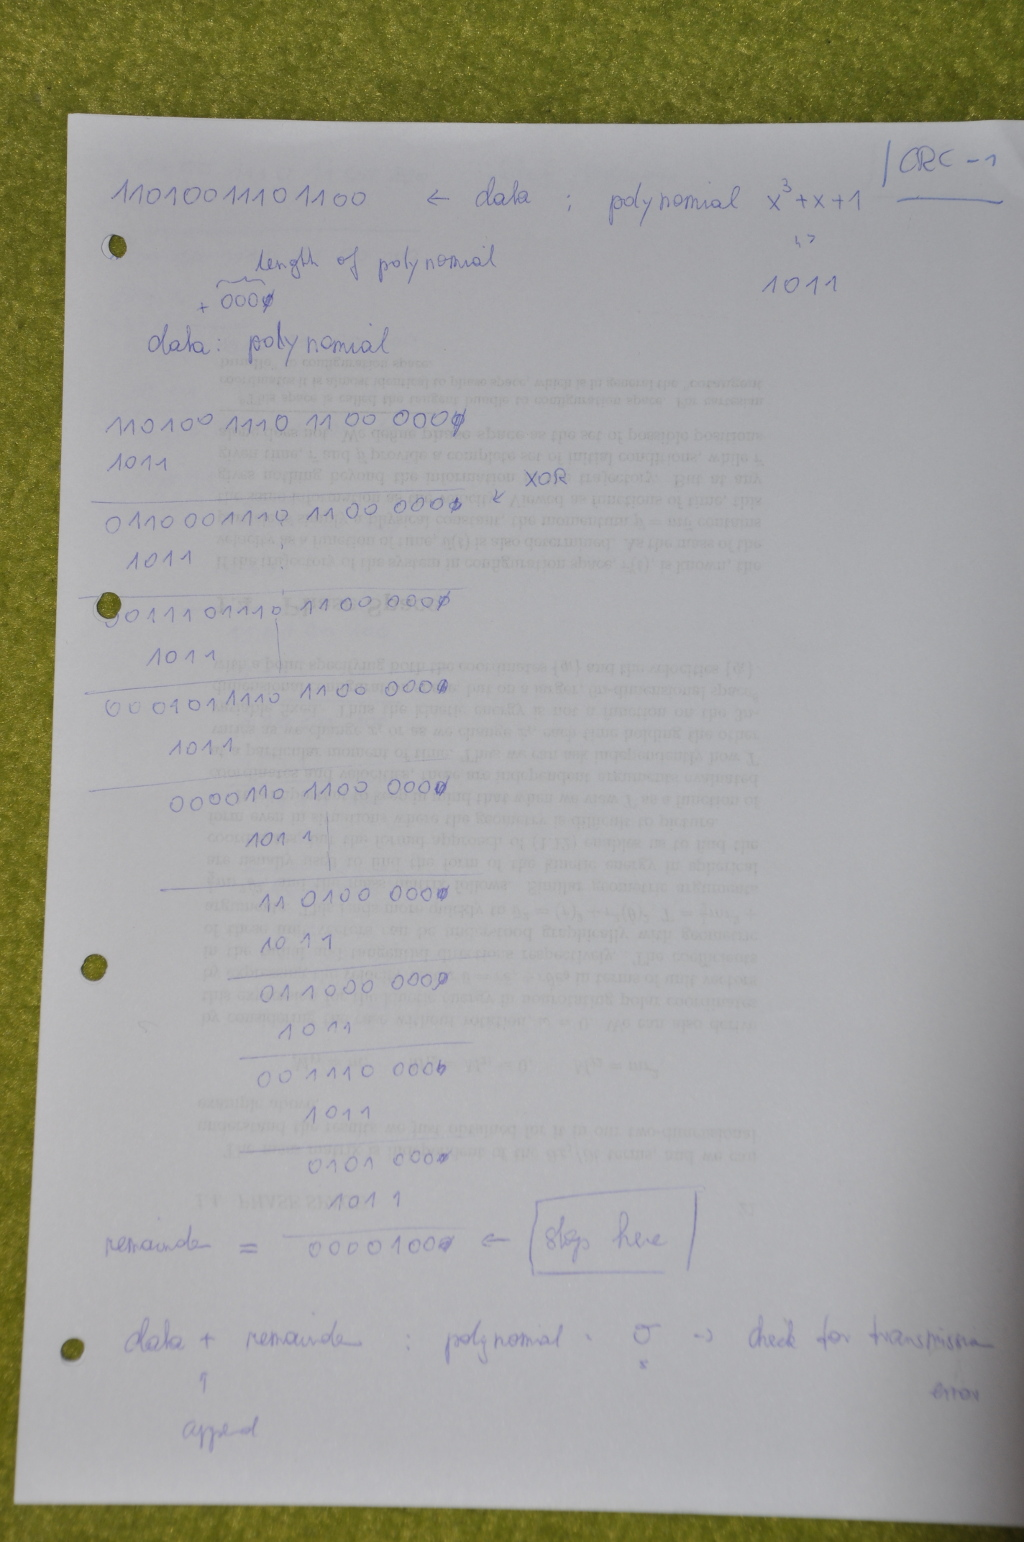
\includegraphics[scale=1.2]{images/DSC_0855_small.JPG}
\end{figure}

Division yields a remainder of \texttt{100} which is the CRC code. We
augment the original dataword with the CRC code to obtain
\texttt{11\ 0100\ 1110\ 1100\ 100}.

\subsection{Decoding Example}\label{decoding-example}

We divide the augmented dataword by the generator polynomial. In case of
no transmission errors, this should yield zero.

\begin{figure}[H]
\centering
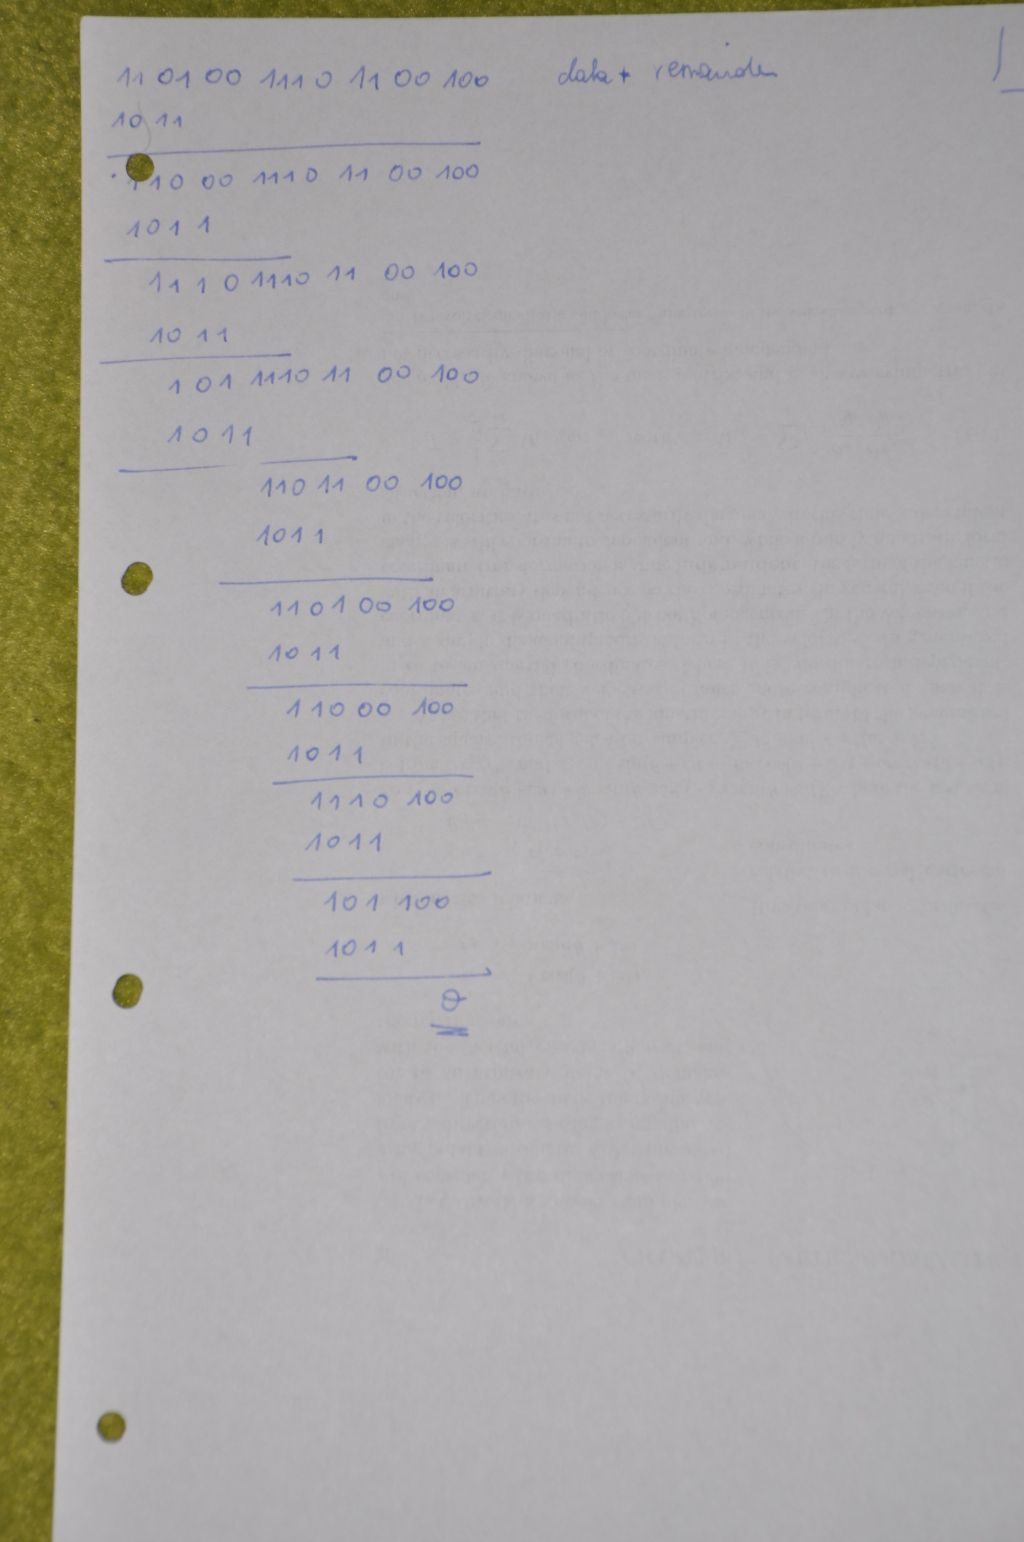
\includegraphics[scale=1.2]{images/DSC_0856_small.JPG}
\end{figure}

\subsection{Julia Example}\label{julia-example}

The (unofficial) Julia Module \texttt{IntModN} provides polynomial
arithmetic over GFs. Below is the example from above solved using this
module.

\begin{verbatim}
include("IntModN.jl")

x=IntModN.X(IntModN.GF2)

w = x^13 + x^12 + x^10 + x^7 + x^6 + x^5 + x^3 + x^2

dw_aug = dw * x^3

# crc code polynomial
p2 = x^3 + x + 1

println(dw_aug)
println(p2)

# divide with remainder; b holds the crc checkword
a, b = IntModN.divrem(dw_aug, p2)

println(a, " ... " , b)

# we finally transmit the dataword augmented with the crc checkword
dw_final = dw_aug + b

# dividing the received dataword by the crc polynomial
c, d = IntModN.divrem(dw_final, p2)

# yields a remainder of zero
println(d)
\end{verbatim}

%\DiaryEntry{Newton Root Finding}{2015-06-28}{Maths}

Find zero(s) for \(f(x)\). The basic idea is to start with a point
\(x_n\) on \(f(x)\) and calculate the tangent \(g(x)\) to the curve at
this point. Find the zero of the tangent \(g(x)\); that's \(x_{n+1}\);
i.e.~the next starting point.

\begin{figure}[hbt!]
\centering
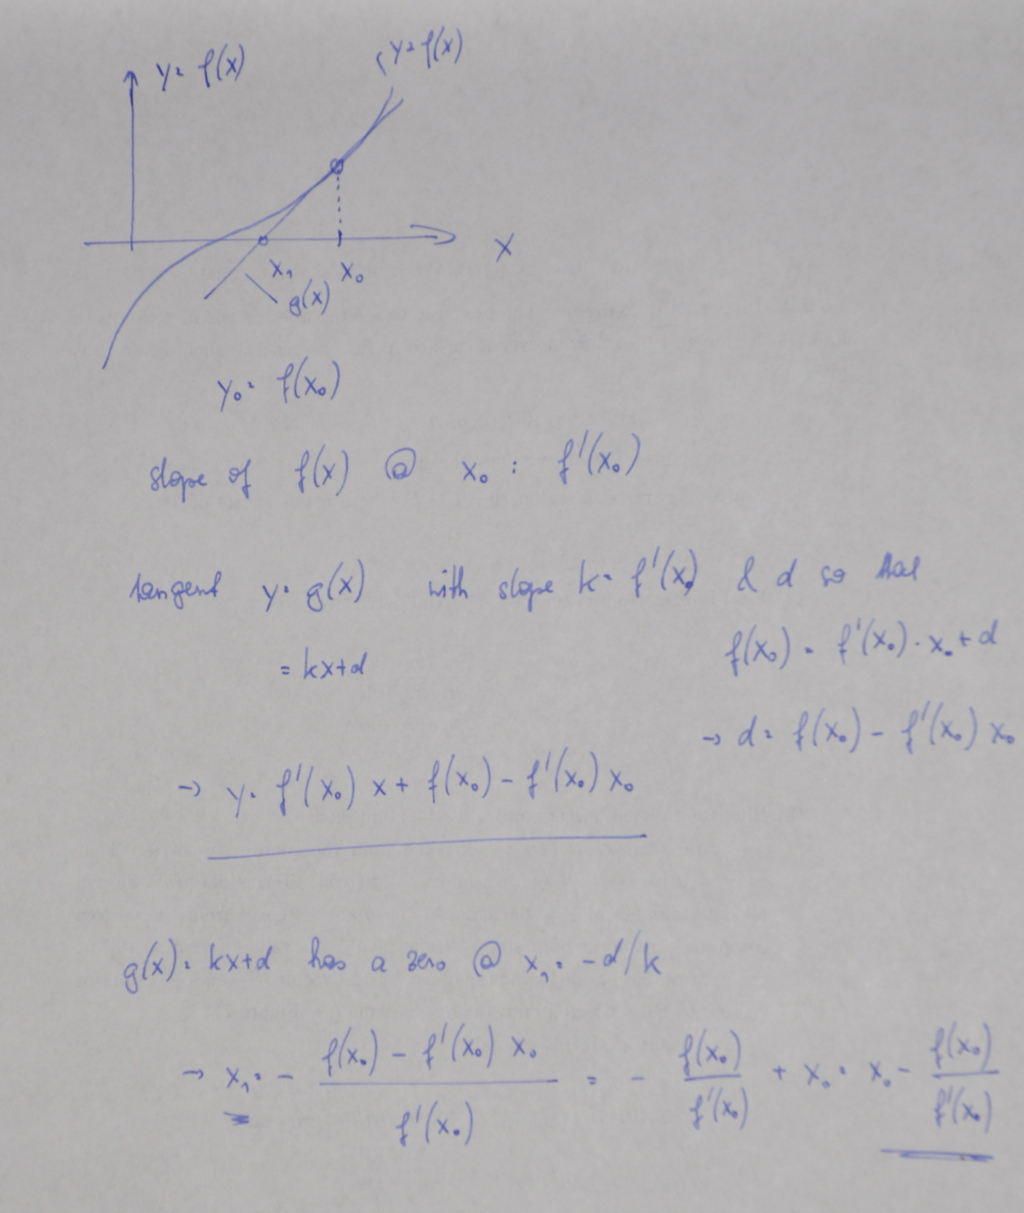
\includegraphics[scale=1.5]{images/DSC_0001_small.JPG}
\caption{Page1}
\end{figure}

e.g. \(f(x) = x^2-4\); then \(f'(x) = 2x\) and
\(x_{n+1} = x_n - (x^2-4)/(2x)\)

see
\href{file:///home/cnovak/src/julia/JuliaStuff/newton.jl}{newton.jl}:

\begin{verbatim}
function newton_solve(z0)
# solve x^2 - 4 = 0
    z = z0
    for n=1:20
        z = z - (z*2-4)/(2*z)
        println(n, " -> ", z)
    end
    return z
end

println(newton_solve(4))
\end{verbatim}

yields

\begin{verbatim}
1 -> 3.5
2 -> 3.0714285714285716
3 -> 2.722591362126246
4 -> 2.457185626921853
5 -> 2.271124947617549
6 -> 2.151745805619235
7 -> 2.0812236253398755
8 -> 2.0421967642419427
9 -> 2.021534326135688
10 -> 2.0108818599087837
11 -> 2.0054703734730377
12 -> 2.0027426475762127
13 -> 2.001373201741756
14 -> 2.000687071968178
15 -> 2.0003436539605324
16 -> 2.0001718564997053
17 -> 2.000085935632882
18 -> 2.000042969662595
19 -> 2.0000214852928857
20 -> 2.000010742761846
2.000010742761846
\end{verbatim}

%\DiaryEntry{Probability of the Union of Events}{2015-07-21}{Stochastic}


Based on
\href{https://terrytao.wordpress.com/2010/01/01/254a-notes-0-a-review-\%20\%5Bof-probability-theory/}{Exercise
15} in Terry Tao's blog.

Two events $E_1, E_2$ with probabilites $P(E_1) = P_1, P(E_2) = P_2$. Below we assume independent events; that is $P(E_1, E_2) = P(E_1) \times P(E_2)$; or, to be more exact $P(E_1=e_1 \cap E_2=e_2) = P(E_1=e_1) \times P(E_2=e_2)$.

\begin{figure}[hbt!]
\centering
\includegraphics[scale=0.5]{images/union_probability.png}
\caption{Page1}
\end{figure}

Similar (probability is proportional to the size of sets), there is the Sieve Formula for calculating the size of the union of sets:

\[ |A_1 \cup A_2 \cup \cdots A_n| = \sum_{j=1}^n (-1)^{j-i} \sum_{i_1, i_2, i_j} | A_{i_1} \cap A_{i_2} \cap \cdots A_{i_j}|\]

where $i_1, i_2, \ldots , i_j$ covers all j-element subsets of $[n]$.

For the case $n=2$, we therefore have

\[ |A_1 \cup A_2| = |A_1| + |A_2| - |A_1 \cap A_2| \]

for $n=3$, we have

\[ |A_1 \cup A_2 \cup A_3 | = |A_1| + |A_2| + |A_3| - |A_1 \cap A_2| - |A_1 \cap A_3| - |A_2 \cap A_3| + |A_1 \cap A_2 \cap A_3| \].

Compare this with the results in the handwritten notes above.

%\DiaryEntry{Gamma Function}{2015-07-27}{Maths}

\subsection{Partial Integration}

First thing is the derivation of the partial integration: We differentiate the product of two functions

\bee
\frac{d (u(x)v(x)}{dx} = u(x) \frac{d v(x)}{dx} + v(x) \frac{d u(x)}{dx}
\eee
%
integrate both sides

\bee
u(x)v(x) = \int u(x) \frac{d v(x)}{dx} dx + \int v(x) \frac{d u(x)}{dx} dx
\eee
%
and rearrange the result so that we obtain
%
\bee
\int u(x) \frac{d v(x)}{dx} dx = u(x)v(x) - \int v(x) \frac{d u(x)}{dx} dx
\eee
%
or - in a more sloppy notation - we have
%
\bee
\int u v' dx = uv - \int u' v dx
\eee

\subsection{Definition and Properties}

The Gamma function $\Gamma(x)$ is defined according to
%
\bee
\Gamma(x) = \int_0^\infty t^{x-1}e^{-t} dt
\eee

The following Figure shows a plot of the integrand for $x=1, x=2, x=3$, respectively. Note that with increasing $x$, the maximum moves to the right and the area under the curve increases.

\begin{figure}[hbt!]
\centering
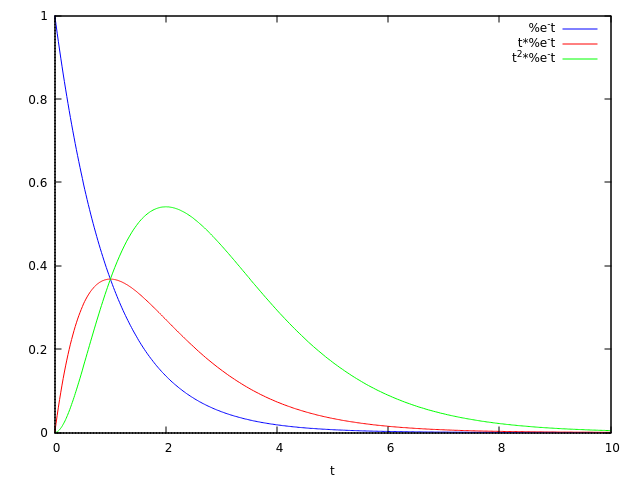
\includegraphics[scale=0.7]{images/gamma_integrand_plot.png}
\end{figure}

\pagebreak

Note, that the Gamma function is also defined for negative values of $x$; the following Figure shows plots of the integrand for $x=-1, x=-2, x=-3$, respectively. It diverges at $t=0$, and falls off for increasing $t$.

\begin{figure}[hbt!]
\centering
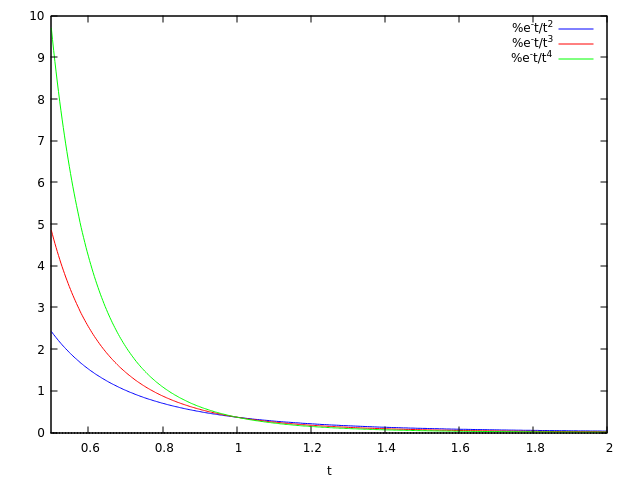
\includegraphics[scale=0.7]{images/gamma_integrand_neg_plot.png}
\end{figure}


The Gamma function fulfills the following recurrence relation
%
\bee
\Gamma(x+1) = x \Gamma(x)
\eee
%
which we can prove as follows
%
\bee
\Gamma(x+1) = \int_0^\infty t^{x}e^{-t} dt
\eee
by partial integration ($v'e^{-t} \rightarrow v = -e^{-t}, u=t^x \rightarrow u'=x t^{x-1}$) we obtain
%
\bee
\Gamma(x+1) = \left. -t^x e^{-t} \right|_0^\infty - \int_0^\infty x t^{x-1}(-1)e^{-t} dt = 0 + \int_0^\infty x t^{x-1}e^{-t} dt = x \int_0^\infty t^{x-1}e^{-t} dt
\eee
%
where in the last step we have used the fact that the integral is over $t$ and therefore $x$ can be taken out of the integral. Comparing with the definition, we see that
%
\bee
\Gamma(x+1) = x \Gamma(x) \qed
\eee
%
Next we calculate the value of $\Gamma(1)$ as
%
\bee
\Gamma(1) = \int_0^\infty t^{0}e^{-t} dt = \int_0^\infty e^{-t} dt = \left. e^{-t} \right|_0^\infty = 1
\eee
%
The function plot looks as follows (be careful; Julia uses a gamma function shifted by one):

\begin{figure}[hbt!]
\centering
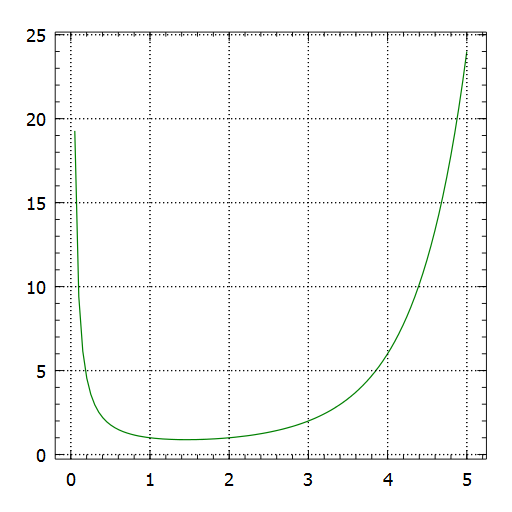
\includegraphics[scale=0.5]{images/gamma_plot.png}
\end{figure}

%\DiaryEntry{Digital Ocean Setup Notes}{2015-07-28}{General}


\subsection{Users}\label{users}

root / das übliche

cno / das übliche

\subsection{Package Installation}\label{package-installation}

\begin{verbatim}
apt-get install <package name>

apt-cache search <search name>
\end{verbatim}

\subsection{CLI Window Manager}\label{cli-window-manager}

\href{https://www.digitalocean.com/community/tutorials/how-to-use-dvtm-and-dtach-as-a-terminal-window-manager-on-an-ubuntu-vps}{Using
dvtm and dtach}

\paragraph{Using dvtm}\label{using-dvtm}

DVTM is a window manager for the console. It allows to manage several
windows (open, close, switch to\ldots{}).

\begin{verbatim}
C-g

    c ... create new window

    j/k ... cycle through open windows

    x ... destroy current window

    q ... destroy all windows and exit

    space ... change window tiling-mode

    m ... switch to full-screen window tiling mode
\end{verbatim}

\paragraph{Using detach}\label{using-detach}

Dtach is like screen for use together with DVTM.

Start / reattach to a session

\begin{verbatim}
dtach -A /tmp/dvtm -r winch dvtm
\end{verbatim}

\subsection{PostgreSQL}\label{postgresql}

Access to standard port 5432 is not possible from FRQ; use an iptable rule to forward connection from localhost:80 to localhost:5432 \href{see:\%20http://serverfault.com/questions/112795/how-can-i-run-a-server-on-linux-on-port-80-as-a-normal-user}{according to this link}.

\begin{itemize}

\item create iptables rule

\begin{verbatim}
iptables -t nat -A PREROUTING -p tcp --dport 80 -j REDIRECT --to-port 5432
\end{verbatim}

\item show rules - chain prerouting

\begin{verbatim}
iptables -t nat --line-numbers -n -L
\end{verbatim}

\item delete rule number N from iptables:

\begin{verbatim}
iptables -t nat -D PREROUTING N
\end{verbatim}


\end{itemize}

%%\section{Markov Inequality, 2015-08-16}
%\label{2015-08-16:entry}

\DiaryEntry{Markov and Chebyshev Inequality}{2015-08-16}{Stochastic}

holds for non-negative random variable $X$ and $a > 0$. Consider an indicator function $I(\cdot)$ which is one when the condition is true and zero otherwise. Now distinguish between the two cases $X \geq a$ and $X < a$. If $X \geq a$, then $I(X \geq a) = 1$; if $X < a$, then $I(X \geq a) = 0$. We can collect this in a single expression, namely
%
\begin{equation*}
a I(X \geq a) \leq X
\end{equation*}
%
Taking expectation on both sides yields
%
\begin{equation*}
a \mathrm{E}(I(X \geq a)) \leq \mathrm{E}(X)
\end{equation*}
%
and we observe that $a \mathrm{E}(I(X \geq a)) = P(X \geq a)$ and therefore we have
%
\begin{equation*}
a P(X \geq a) \leq \mathrm{E}(X) \rightarrow P(X \geq a) \leq \frac{\mathrm{E}(X)}{a}
\end{equation*}
%
which is the famous Markov inequality.


\subsection*{Example}

Example for the exponential distribution $f(x) = \lambda e^{- \lambda x}$ as follows:
%
\begin{equation*}
P(X \geq a) =  \int_a^\infty \lambda e^{- \lambda x} = e^{- \lambda a}
\end{equation*}
%
The expectation is $E(X) = 1/\lambda$ and therefore we have
%
\begin{equation*}
P(X \geq a) \leq \frac{1}{\lambda a}
\end{equation*}
%
In the plot below the green curve shows the true value of $P(X \geq a)$; the blue curve is the Markov approximation.

\begin{figure}[h]
\centering
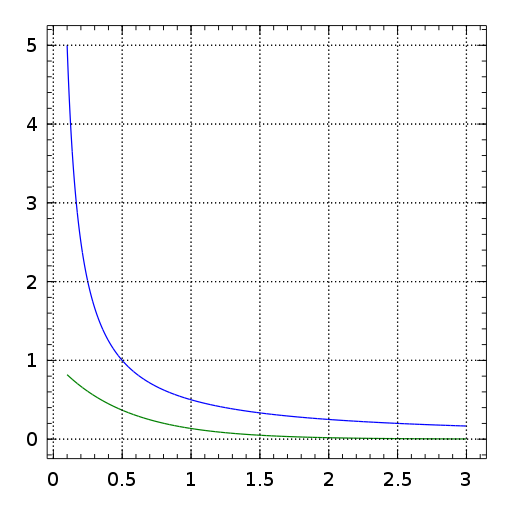
\includegraphics[scale=0.35]{images/exponential.png}
\caption{Exponential Distribution: Tail probabilities.}
\end{figure}

\subsection*{Chebyshev Inequality}

Whereas the Markov inequality holds only for positive RV's and requires only a known mean, the Chebyshev inequality holds for any RV with known (and existing) mean and variance.

We consider the absolute value of a RV $|X|$. Using the Markov inequality, we have
%
\begin{equation*}
  P(|Y| \geq a) \leq \frac{\mathrm{E}\{|Y|\}}{a}
\end{equation*}
%
We now consider a RV $Y = (X - \mu)^2$ and $a = (k \sigma)^2$ (where $\mu$ is the expectation of $X$ and $\sigma^2$ its variance) and we obtain
%
\begin{equation*}
  P(|X-\mu|^2 \geq (k \sigma)^2) \leq \frac{\mathrm{E}\{(X-\mu)^2\}}{(k \sigma)^2} = \frac{\sigma^2}{k^2 \sigma^2} = 1 / k^2
\end{equation*}
%
%
We therefore arrive at the Chebyshev inequality
%
\begin{equation*}
    P(|X-\mu|^2 \geq (k \sigma)^2) \leq 1 / k^2
\end{equation*}
%
or
%
\begin{equation*}
    P(|X-\mu| \geq k \sigma) \leq 1 / k^2
\end{equation*}


\subsubsection*{Example: Normal Distribution}

Normal distribution with zero mean $\mathcal{N}(0, \sigma^2)$. $P(X \leq x) = F(x) = \frac{1}{2} \left[ 1 + \erf \frac{x}{\sigma\sqrt{2}} \right]$ (see \href{https://en.wikipedia.org/wiki/Normal_distribution}{Wikipedia}). Then $P(|X| \geq a) = 2 F(-a)$ or $P(|X| \geq k\sigma) = 2 F(-k\sigma) = 1 + \erf \frac{-k}{\sqrt{2}}$, which ``interestingly'' does not depend on $\sigma$ but only on $k$.
%
The bound using Chebyshev's inequality states that $P(|X| \geq k \sigma) \leq 1/k^2$.

\subsubsection*{Example: Mean of RVs}

We have $N$ iid RVs with mean \(\mu_x\) and variance \(\sigma_x^2\) and calculate the mean
%
\begin{equation*}
M = \frac{1}{N} \sum_i x_i
\end{equation*}
%
which has mean \(E\{M\} = \frac{1}{N} N \mu_x = \mu_x\) and variance \(E\{(M-\mu_x)^2\} = \frac{\sigma_x^2}{N}\). Using Chebyshev's inequality, we have
%
\begin{equation*}
P \left(| X-\mu_x |^2 \geq k^2 \frac{\sigma_x^2}{N} \right) \leq \frac{1}{k^2}
\end{equation*}
%
Now we can set \(\alpha = k^2 \frac{\sigma_x^2}{N}\) (and therefore \(\frac{1}{k^2} = \frac{\sigma_x^2}{\alpha N}\)) and finally obtain
%
\begin{equation*}
P \left(| X-\mu_x |^2 \geq \alpha \right) \leq \frac{\sigma_x^2}{\alpha N}
\end{equation*}
%
By considering ``enough'' RVs in the mean calculation, we can make the deviation of \(M\) arbitrarily small around the mean \(\mu_x\).

%\DiaryEntry{Normal Distribution}{2015-08-17}{Stochastic}

A short summary of things I keep forgetting, mostly based on \href{https://en.wikipedia.org/wiki/Normal_distribution}{Wikipedia}.
%
Normal distribution with mean $\mu$ and variance $\sigma^2$: $\Nc(\mu, \sigma^2)$.

\subsection{PDF}\label{pdf}

The pdf has the following form:

\[f(x) = \frac{1}{\sqrt{2\pi\sigma^2}} e^{ - \frac{(x-\mu)^2}{2\sigma^2} }\]

\subsection{CDF}\label{cdf}

The CDF $F(x)$ gives the probability $P(X < x ) = F(x)$. There is no closed form available; use the error function instead:

\[\text{erf}(x) = \frac{1}{\pi} \int_{-x}^x e^{-t^2/2}\]
%
The error function gives the probability of a normal RV with zero mean variance $1/2$ falling into the range $[-x;x]$.
%
With this we obtain for a RV with normal distribution $\mathcal{N }(\mu, \sigma^2)$:

\[F(x) = P(X < x)  = \frac{1}{2} \left[ 1 + \text{erf} \left( \frac{x-\mu}{\sqrt{2\sigma^2}} \right) \right] \]
%
In Julia we can do this as follows:

\begin{verbatim}
# generate N random normal RVs
N = 1000000

# with variance s2
s2 = 1.5

x = sqrt(s2)*randn(N)

# find the prob of X < xlim
xlim = 1.2

# empirically
println(count(x->x<xlim, x)/N)

# with the error function
trueval = 0.5*(1+erf(xlim/(sqrt(2*s2))))
\end{verbatim}
%
By the way, note the elegant way of counting the elements of the vector \texttt{x} which are less than \texttt{xlim}. Using these definitions, we can also calculate other probabilities; e.g.
%
\[P(a < X < b) = F(b) - F(a); \qquad b > a\]
%
Empirically measured in Julia via \texttt{println(count(x-\textgreater{}x\textgreater{}a\ \&\&\ x\textless{}b,\ x)/N)}. Another probability is
%
\[P(X > a) = 1 - F(a),\]
%
empirically measured in Julia via \texttt{println(count(x-\textgreater{}x\textgreater{}a,\ x)/N)}.

%\DiaryEntry{Geometric Distribution}{2015-08-18}{Stochastic}

Two definitions, but the same principle: Number of Bernoulli trials, before the trial succeeds.

The success probability of the Bernoulli trial is denoted by $p$; the random variable $X$ denotes the number of trials $k$ before a trial succeeds and therefore has a pmf as follows:

\[ P(X=k) = (1-p)^k p\]

\subsection{Expectation}

The expectation $\mathcal{E}(X)$ is calculated as follows

\[\mathcal{E}(X) = \sum_{k=0}^\infty k \times P(X=k) = \sum_{k=0}^\infty k (1-p)^k p \]

We can rewrite this as

\[\mathcal{E}(X) = p(1-p) \sum_{k=0}^\infty k (1-p)^{k-1} \]

and realize that the summand can be written as differential

\[k(1-p)^{k-1} = - \frac{d}{dp} (1-p)^k\]

Exchanging summation with differentiation, we obtain

\[\mathcal{E}(X) = -p(1-p) \frac{d}{dp} \sum_{k=0}^\infty (1-p)^k \]

The sum is the geometric series
$\sum_{k=0}^\infty q^k = \frac{1}{1-q}$ with $q=1-p$, and we therefore have

\[\mathcal{E}(X) = -p(1-p) \frac{d}{dp} \frac{1}{p} = p(1-p)\frac{1}{p^2} = \frac{1-p}{p}\]

For small $p$, the expectation is large; i.e.~it takes a long time, before the trial succeeds. If $p=1/2$, $\mathcal{E}(X)=1$; i.e.~success is reached after 1 trial. Finally for $p=1, \mathcal{E}(X)=0$.

\subsection{Example}

Consider a dice with probability $p=1/6$ that one side comes up (e.g.~6). Then the RV $X$ denotes the number of trials, before this side comes up. The expectation is $\mathcal{E}(X) = \frac{1-p}{p} = \frac{5/6}{1/6} = 5$; i.e.~it takes 5 rolls, \textbf{before} this side comes up. In other words, on average, the 6-th roll shows the side.

\subsection{Sequences}

Consider a sequence of such trials: After a successful trial, the process is started again ad infinitum. The average time between successes (and therefore process restarts) is $\mathcal{E}(X)$. Therefore a length-N sequence contains $1/\mathcal{E}(X)$ successful trials.

%\DiaryEntry{Differentiate Trigonometric Functions}{2015-08-25}{Maths}


\subsection{Prerequisites}

\subsubsection{Expansion}

We want to expand $\sin(x+y)$ and $\cos(x+y$. Use complex functions as follows:

\[\cos(x+y) + j \sin(x+y) = e^{j(x+y)} = e^{jx} e^{jy} = \left( \cos x + j\sin x \right) \left( \cos y + j\sin y \right) \]

Expanding the last expression yields

\[ \cos x \cos y - \sin x \sin y + j \left( \cos x \sin y + \sin x \cos y \right) \]

and by comparing real and imaginary parts we obtain

\[\cos(x+y) = \cos x \cos y - \sin x \sin y \]

and

\[ \sin(x+y) = \cos x \sin y + \sin x \cos y \]

\subsubsection{Differentiate Inverse (Trigonometric) Functions}

The trick is to treat the derivative $\frac{dy}{dx}$ like a fraction; e.g.~if $x$ is the independent variable $y=g(x)$ and $\frac{dy}{dx} = g'(x)$, we can obtain the derivative of the inverse function (where $y$ is the independent variable) as $\frac{dx}{dy} =1 /g(x)$. This expression depends on $x$, though; by substituting $x=g^{-1}(y)$, we obtain the derivative $\frac{dx}{dy}$ depending
on $y$. Writing these steps into one, we get

\[ \left( g^{-1}(y) \right)' = \frac{1}{g'(g^{-1}(y))}\]

\subsection{Basic Trigonometric Functions}

We want to calculate $\frac{d \cos x}{dx}$. Use the definition

\[\frac{d \cos x}{dx} = \lim_{\delta \rightarrow 0} \frac{\cos(x+\delta) - \cos x}{\delta}\]

We can expand the expression in the limit as follows

\[\frac{\cos(x+\delta) - \cos x}{\delta} = \frac{\cos x \cos \delta - \sin x \sin \delta - \cos x}{\delta}\]

To obtain the limit, we use the trigonometric series expansions for dmall x $\cos x = 1 - x +
\mathcal{O}(2)$ and $\sin x = x + \mathcal{O}(2)$,

\[\frac{\cos(x+\delta) - \cos x}{\delta} = \frac{ (1 - \delta) \cos x - \delta \sin x - \cos x}{\delta}\]

Now we can calculate the limit

\[\lim_{\delta \rightarrow 0} \frac{ (1 - \delta) \cos x - \delta \sin x - \cos x}{\delta} = - \sin x\]

and therefore we have $\frac{d \cos x}{dx} = -\sin x$. The same approach works for $\frac{d \sin x}{dx} = \cos x$.

A bit more interesting is $\frac{d \tan x}{dx}$ which can be expressed as

\[ \frac{d}{dx} \frac{\sin x}{\cos x} = \frac{\cos^2 x + \sin^2 x}{\cos^2 x} = 1 + \tan^2 x\]

\subsubsection{arctan}

Consider $\frac{d \arctan x}{dx}$ which we can differentiate as follows: We have $y=\tan x$ and know that $\frac{dy}{dx}= 1 + \tan^2 x$ (see Section above). Using the trick from above, we obtain

\[ \frac{dx}{dy} = \frac{1}{1 + \tan^2 x} \]

But we are interested in calculating $\frac{dx}{dy}$  as a function of $y$, so we have to substitute $
x=\arctan y$

\[ \frac{dx}{dy} = \frac{1}{1 + \tan^2 (\arctan y)} = \frac{1}{1 + y^2} \]

which is the desired result.

\subsubsection{arcsin}

The same trick works with $\frac{d \arcsin x}{dx}$. We have $y=\arcsin x$ and $x = sin y =
\sqrt{1 - \cos^2 y}$. Basic manipulations yield $\cos y = \sqrt{1 - x^2}$. Then $\frac{dx}{dy} = \cos y$  and we obtain

\[ \frac{dy}{dx} = \frac{1}{\cos y} = \frac{1}{\sqrt{1 - x^2}} \]

%\DiaryEntry{Random Processes}{2015-08-30}{Stochastic}

This post is based on
\href{http://www.math.uah.edu/stat/poisson/index.html}{this link}.

\subsection{Definitions}\label{definitions}

Consider a random process with ``arrivals'' that occur randomly in time.

Let \(X_i\) denote the time between the arrivals, the inter-arrival times. The arrival times are not constrained to begin integers; therefore the inter- arrival times are real numbers (and the random variable is a continuous one). The first point is at \(X_0\), the second point is \(X_1\) \emph{after} the first one and so on. \(X = (X_0, X_1...\) is the sequence of inter-arrival times.

Let \(T_i\) denote the arrival times with \(T_0=0\). \(T_1\) is the arrival time of the first point, \(T_2\) the arrival time of the second and so forth.

Therefore, we have:

\[ T_n = \sum_{i=0}^n X_i\]

and

\[ X_n = T_n - T_{n-1}\]

Let \(N_t\) denote the number of arrivals in the interval $(0,t)$. This number can be defined as

\[N_t \geq n  \Leftrightarrow T_n \leq t \]

for n (integer) and t (real number) positive. This is a discrete random variable and the underlying process is called a \emph{counting process}.

\subsection{Strong Renewal Property}\label{strong-renewal-property}

Consider a fixed time t. If a random process after this time is independent of the process before this time (i.e.~the process before t and after t behaves probabilistically the same), the random process has a strong renewal property.

The strong renewal property states that at each arrival time and at each fixed time, the process must probabilistically restart independent of the past. This implies that the \(X_i\) are a sequence of independent, identically distributed variables. Furthermore, if the first arrival has not occurred by time s, then the time remaining until the arrival occurs must have the same distribution as the first arrival time itself. This is known as the memoryless property:

\[ P(X>t+s|X>s) = P(X>t)\]

\subsection{Poisson Process}\label{poisson-process}

\subsubsection{\texorpdfstring{Distribution of
\(X_i\)}{Distribution of X\_i}}\label{distribution-of-x_i}

The assumption of a memoryless process is a rather strict assumption in that it restricts the distribution of \(X_i\) to the exponential distribution as follows: The conditional probability \(P(X>t+s|X>s)\) can be rewritten as

\[P(X>t+s|X>s) = \frac{P(X>t+s, X>s)}{P(X>s)} = \frac{P(X>t+s)}{P(X>s)}\]

and memorlessness yields

\[ P(X>t+s) = P(X>t)P(X>s) \]

For \(t=s=1\) we have \(P(X>2 = P(X>1)^2\) and in general we have

\[P(X>a) = P(X>1)^a\]

The only pdf which satisifes this property is the exponential distribution

\[ f_X(u) = r e^{-ru}\]

For this distribution

\[P(X>a) = \int_a^\infty r e^{-ru} = r e^{-ru}|_a^\infty=r e^{-ra}\]

We have \(P(X>1)=e^{-r}\) and therefore

\[ P(X>1)^a = \left( e^{-r} \right)^a = e^{-ra} \]

which proves the claim. Note that the distribution $f_X(u)$ holds for \emph{all} \(X_i\) and is (therefore) independent of \(i\).

\emph{Note: The moments of the exponential distribution are $\mathbb{E}(X^n) = n!/r^n$. Therefore the mean is \(1/r\) and the variance is \(1/r^2\).}

\subsubsection{\texorpdfstring{Distribution of \(T_n\)}{Distribution of T\_n}}\label{distribution-of-t_n}

With this distribution, the distribution of \(T_n = \sum_{i=0}^n X_i\)
follows a gamma distribution with rate parameter r and scale parameter
n:

\[ f_{T_n}(u) = r^n \frac{u^{n-1}}{(n-1)!}e^{-ru}\]

This can be easily shown using moment generating functions (MGFs). The
MGF of the random variable \(X_i\) is given as
\(\text{MGF}_X(t) = \frac{r}{r-t}\). The MGF of \(T_n\) is then given as

\[\text{MGF}_T(t) =  \text{MGF}_X(t)^n = \left( \frac{r}{r-t} \right)^n\]

This MGF corresponds to a gamma distribution with rate parameter r and
scale parameter n.

\emph{Note: The distribution of \(T_n\) depends on n.}

The figure below shows the gamma distribution for n=1, 2, and 5. The
larger n is, the further the peak of the distribution is to the right
and the ``broader'' the peak is. This makes sense, because larger n
means more terms in the sum for \(T_n\).

\begin{figure}[!hbt]
\centering
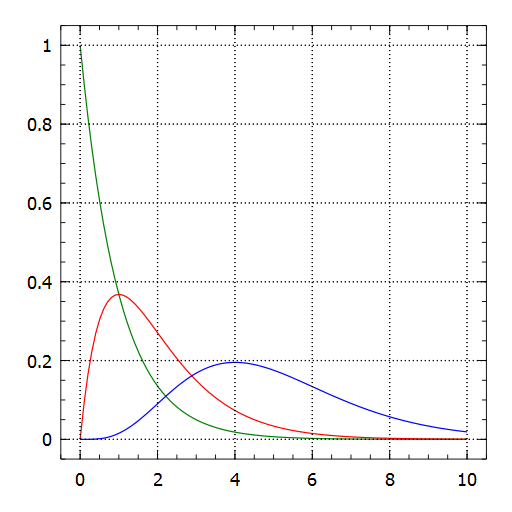
\includegraphics[scale=0.5]{images/gamma_dist_plot.png}
\caption{Page1}
\end{figure}

\subsubsection{\texorpdfstring{Distribution of
\(N_t\)}{Distribution of N\_t}}\label{distribution-of-n_t}

\(N_t\) is defined as the number of arrivals in the intervall $(0,t)$ (see above). By the relation $N_t \geq n \Leftrightarrow T\_n \leq t$, we have

\[ P(N_t \leq n) = P(T_n \leq t) = \int_0^t r^n \frac{u^{n-1}}{(n-1)!}e^{-ru} du \]

This integral can be calculated as (table book)

\[ P(N_t \leq n) = 1 - e^{-rT} \sum_{k=0}^{n-1} \frac{(rT)^k}{k!}\]

Considering integer values for \(n\), we can write
\(P(N_t=n)=P(N_t \geq n)-P(N_t \geq n+1)\). Inserting above expression,
we finally obtain

\[ P(N_t=n) = e^{-rt} \frac{(rt)^n}{n!}\]

which is the Possin distribution with parameter \(rT\). It is
interesting, that it only depends on the product of r and T and not on
the parameters separately. Because it describes a counting process,
\(N_t\) is a discrete random variable.

%\DiaryEntry{Generating Functions, Part 1}{2015-09-09}{GenFuncs}


Based on Concrete Mathematics.

\subsection{Definition}\label{definition}

The generating function of a time-discrete sequence $\{g\_n\}, n=0\ldots{}\infty$ has the following form

\[ G(z) = z^0 g_0 + z^1 g_1 + z^2 g_2 + \cdots = \sum_{n \geq 0} g_n z^n\]

\subsubsection{Application to Recurrence Relations}

The most prominent usage of generating functions is to find closed-form expressions for recurrence relations.

\begin{itemize}
\item
  First write down the sequence \({g_n}, n=0...\infty\); i.e.~express
  \$g\_n \$ in terms of other elements of the sequence. This expression
  shall be valid for \emph{all} n, assuming that \(g_n=0\) for
  \(n < 0\).
\item
  Multiply both sides of the equation with z\^{}n and sum over all n. On
  the left side of the equation this gives \(G(z)\); the right side
  becomes ``something else''.
\item
  Find a closed form expression for \(G(z)\) and expand this expression
  into a power series. Read off the coefficients of \(z^n\).
\end{itemize}

\subsection{Simple Examples}

\subsubsection{\texorpdfstring{\(g_n=\alpha^n\)}{g\_n=\textbackslash{}alpha\^{}n}}

We have a recurrence relation \(g_n=\alpha g_{n-1}\) with the inital
condition \(g_0=1\).

We have

\[\sum_n g_n z^n = \sum_n \alpha g_{n-1} z^n + 1\]

which we can simplify to

\[G(z) = \alpha \sum_n g_{n} z^{n+1} + 1 = \alpha z \sum_n g_n z^n +1 = \alpha z G(z) + 1\]

This yields the following expression for the generating function

\[ G(z) = \frac{1}{1-\alpha z} \]

and corresponds to the sequence $g_n = \alpha^n$.

\subsubsection{\texorpdfstring{\(g_n=-\alpha^n\)}{g\_n=-\textbackslash{}alpha\^{}n}}\label{g_n-alphan}

We have (with the initial condition \(g_0=1\))

\[\sum_n g_n z^n = -\alpha \sum_n g_{n-1} z^n + 1\]

which yields for the generating function $G(z) = \frac{1}{z+\alpha}$. We can rewrite it as follows:

\[G(z) = \frac{1}{\alpha} \frac{1}{1 + x/\alpha} = \frac{1}{\alpha} \frac{1}{1 - x/(-\alpha)} \]

This function corresponds to the sequence \(g_n = (-\alpha)^n\).

\subsection{Fibonacci Numbers Example}\label{fibonacci-numbers-example}

Define \(g_n\) as

\[ g_n = g_{n-1} + g_{n-2} + [n=1] \]

where the expression \([n=1]\) is one when n=1 and zero otherwise. This
is an expression for \(g_n\) valid for all n (positive and negative).

Executing steps \#2, we obtain

\[ \sum_n g_n z^n = \sum_n g_{n-1} z^n + \sum_n g_{n-2} z^n  + \sum_n [n=1] z^n \]

Keeping in mind that this epxression is valid for \emph{all} n, we can
shift the summation indices in order to obtain

\[ \sum_n g_n z^n = \sum_n g_{n} z^{n+1} + \sum_n g_{n} z^{n+2}  + \sum_n [n=1] z^n \]

The last sum yields \(z\) and we finally obtain

\[ \sum_n g_n z^n = z \sum_n g_{n} z^n + z^2 \sum_n g_{n} z^n + z \]

This form allows a closed-form expression for the generating function as

\[ G(z) = z G(z) + z^2 G(z) + z \]

and we arrive at

\[ G(z) = \frac{z}{1-z-z^2} \]

We can make a partial fraction expansion to get a closed-form expression
or we throw the expression at \texttt{sympy}, Wolfram Alpha etc to get a
series expansion.

With sympy, this works as follows:

\begin{verbatim}
import sympy as sym

x, n = sym.symbols("x n")
F = x / (1-x-x**2)
res = sym.series(F, x, 0, 10)

sym.pprint(res)
\end{verbatim}

and results in

\begin{verbatim}
     2      3      4      5      6       7       8       9    / 10\
x + x  + 2*x  + 3*x  + 5*x  + 8*x  + 13*x  + 21*x  + 34*x  + O\x  /
\end{verbatim}

The coefficients are the Fibonacci numbers with
\(g_0=0, g_1=1, g_2=1, g_3=2 \ldots\).

To see the effect of the inital condition, we can start with \(g_0=1\);
in this case we have

\[ g_n = g_{n-1} + g_{n-2} + [n=0] \]

and

\[ \sum_n g_n z^n = z \sum_n g_{n} z^n + z^2 \sum_n g_{n} z^n + 1 \]

Therefore, the generating function becomes $G(z) = \frac{1}{1-z-z^2}$ and a series expansion yields

\begin{verbatim}
           2      3      4      5       6       7       8       9    / 10\
1 + x + 2*x  + 3*x  + 5*x  + 8*x  + 13*x  + 21*x  + 34*x  + 55*x  + O\x  /
\end{verbatim}

These are the Fibonacci numbers again, but shifted by to the right by one.

%\DiaryEntry{Generating Functions, Part 2}{2015-09-07}{GenFuncs}

\subsubsection{Using Partial Fraction
Expansion}\label{using-partial-fraction-expansion}

We continue with the generating function

\[ G(z) = \frac{z}{1-z-z^2} \]

and with the goal to expand it into partial fractions. To this end we
factor the denominator

\[G(z) = - \frac{z}{z^2 - z + 1} =  - \frac{z}{(z-r_+)(z-r_{-} )} \]

with $r_+=\frac{1}{2}(-1+\sqrt{5})$ and $r_{-}=\frac{1}{2}(-1-\sqrt{5})$.

Since $r_+ \neq r_-$, the partial decomposition becomes

\[G(z) = -\left( \frac{A}{z-r_+} + \frac{B}{z-r_{-}} \right) \]

Multiplying both sides with $(z-r_+)(z-r_-)$, we obtain

\[z = A(z-r_{-}) + B(z-r_+)\]

and from that the following two equations

\[A + B = 1, \quad A r_{-} + B r_{+} = 0\]

Solving for $A$ and $B$, we get

\[A = \frac{r_+}{r_{+} - r_{-}}, \quad B = -\frac{r_{-}}{r_{+} - r_-} \]

and therefore the generating function becomes

\[G(z) = - \frac{1}{r_{+} - r_-}\left(  \frac{r_+}{z-r_+} - \frac{r_-}{z-r_-} \right)\]

Anticipating that we need for the backtransform denominators of the form
$(1-z_\rho$), we rewrite the expression as
follows

\[G(z) = \frac{1}{r_{+} - r_-}\left( \frac{1}{1-z/r_+} - \frac{1}{1 - z/r_-} \right) \]

So far, the whole expansion did not take the values of the roots $r_+$ and $r_-$ into account; in order to proceed we note that $r_+ - r_- = \sqrt{5}$, $\phi_+ = \frac{1}{r_+}=\frac{1+\sqrt{5}}{2}$, and $\phi_- = \frac{1}{r_-}=\frac{1-\sqrt{5}}{2}$. With this we finally get

\[G(z) = \frac{1}{\sqrt{5}} \left( \frac{1}{1-z \phi_+} - \frac{1}{1 - z \phi_-} \right) \]

A geometric series$ 1 =q^0, q^1,q^2 \ldots$ has the following sum $\sum_{n \geq 0}q^n = \frac{1}{1-q}$; therefore the generating function can be written as an infinite sum

\[G(z) = \frac{1}{\sqrt{5}} \left( \sum_{n \geq 0} (z \phi_+)^n - \sum_{n \geq 0} (z \phi_-)^n \right) \]

From this we see that the sequence $g_n$ has the following form

\[g_n = \frac{1}{\sqrt{5}} \left( \phi_+^n - \phi_-^n \right) \]

Interestingly, even though there are a lot of irrational numbers in the expression, it yields the Fibonacci sequence $g_n=(0,1,1,2,3,5\ldots$.

%\DiaryEntry{Generating Functions, Part 3}{2015-09-07}{GenFuncs}

The idea is to construct rules which allow a simple calculation of the generating function.

\subsection{Shifting Sequences}\label{shifting-sequences}

Assume we have a generating function $G(z)$ corresponding to a sequence $a_n$. We will denote this correspondence as $a_n \leftrightarrow A(z)$

\[G(z) = a_0 + a_1 x + a_2 z^2 + \cdots = \sum_{n \geq 0} a_n z^n\]

If we shift the sequence to the right; i.e. $a_{n+1}$, we obtain for the generating function

\[\sum_{n \geq 0} a_{n+1} z^n = \frac{1}{z} \sum_{n \geq 0} a_{n+1} z^{n+1} = \frac{1}{z} \sum_{n \geq 1} a_{n} z^{n} \]

The last sum is ``almost'' the generating function; we can change the summation index and obtain

\[ \frac{1}{z} \sum_{n \geq 1} a_{n} z^{n} = \frac{1}{z} \left( \sum_{n \geq 0} a_{n} z^{n} - a_0 \right) = \frac{A(z) - a_0}{z}\]

I.e. $a_{n+1} \leftrightarrow \frac{A(z)-a_0}{z}$. Playing this trick several times we obtain the following correspondence

\[ a_{n+k} \leftrightarrow \frac{A(z) - a_0 - a_1 z - \cdots - a_{k-1}z^{k-1}}{z^k}\]

A shift in the other direction (i.e.~to the left) is also possible. In this case we consider the sequence $a_{n-k}$ and for the corresponding generating function we obtain

\[ \sum_{n \geq 0} a_{n-k} z^n = z^k \sum_{n \geq 0} a_{n-k} z^{n-k} = z^k A(z) \]

The underlying assumption of this derivation is that $a_0 \cdots a_{k-2} = 0$, and only $a_{k-1}$ is allowed to be unequal zero: $a_{k-1} \neq 0$.


\subsubsection{Example}\label{example}

With this rule, we can obtain the generating function for the Fibonacci sequence $a_{n+2} = a_{n+1} + a_n$ as follows

\[ \frac{A(z) - a_0 - a_1 z}{z^2} = \frac{A(z)-a_0}{z} + A(z)\]

Inserting the initial conditions $a_0=0, a_1=1$ yields

\[ \frac{A(z) - z}{z^2} = \frac{A(z)}{z} + A(z)\]

from which we obtain the generating function

\[ A(z) = \frac{z}{1-z-z^2} \]

which is exactely the same as in part 1 of this series.

Considering general initial conditions yields the general generating function

\[ A(z) = \frac{a_0 + (a_1 -a_0) z}{1-z-z^2} \]

For the initial conditions $a_0=a_1=1$ we obtain $A(z) = \frac{1}{1-z-z^2}$ which corresponds to the result in part 1 of this series. In the general generating function the denominator does not depend on the initial conditions and the roots $r_-, r_+$ (see part 2 of the series) are the same as well. Therfore the ``overall structure'' of the corresponding sequence $a_n=\phi_+^n - \phi-^n$ will be independent of the inital conditions.

\subsection{Differentiation}\label{differentiation}

When we have $A(z) = \sum_{n \geq 0} a^n z^n$ and we take the deriative (with respect to z), we obtain

\[A'(z) = \sum_{n \geq 0} n a^n z^{n-1}\]

Adding a $z$, we find the correspondence

\[z A'(z) = \sum_{n \geq 0} n a^n z^n\]

therefore $z A'(z) \leftrightarrow n a\_n$. Playing this trick several times, we find the general relation

\[\left( z \frac{d}{dz} A(z) \right)^k = \sum_{n \geq 0} n^k a^n z^n\]

Be careful with the notation here; for example we have

\[ z \frac{d}{dz} z \frac{d}{dz} A(z) = \sum_{n \geq 0} n^2 a^n z^n \]

\subsubsection{Example 1}\label{example-1}

This example shows the use of differentiation and that a generating function can be evaluated at a certain point $z$ in a meaningful manner.

We have

\[ \sum_{n=0}^N x^n = \frac{x^{N+1}-1}{x-1} \]

Differentiating both sides and multiplying with $x$ yields

\[ \sum_{n=0}^N n x^n = x \frac{d}{dx} \frac{x^{N+1}-1}{x-1} \]

We can now calculate this expression for a fixed value of $x=1$ to obtain

\[ \sum_{n=0}^N n = \lim_{x \rightarrow 1} \left( x \frac{d}{dx} \frac{x^{N+1}-1}{x-1} \right) =\frac{N(N+1)}{2} \]

The last step required some tedious algebra, this was solved by means of sympy

\begin{verbatim}
import sympy as sym

x, n = sym.symbols("x n")

f = (x**(n+1)-1)/(x-1)
g = sym.diff(f, x)
res = sym.limit(x*g, x, 1)

sym.pprint(res)
\end{verbatim}

\subsubsection{Example 2}\label{example-2}

Consider the series described by $(n+1) a_{n+1} = a_n$ with $a_0=1$. Calculate the generating function of the LHS according to

\[ \sum_{n \geq 0} (n+1) a_{n+1} z^n = \frac{d}{dz} \sum_{n \geq 0} a_{n+1} z^{n+1} = \frac{d}{dz} \sum_{n \geq 0} a_{n} z^{n} - a_0 = \frac{d}{dz} \left( A(z) - a_0 \right) \]

But $a_0$ is independent of $z$; therefore the generating function of the LHS becomes $\frac{d}{dz} A(z)$. The generating function of the complete series is

\[\frac{d}{dz} A(z) = A(z)\]

and therefore $A(z) = c e^z$. Series expansion yields

\[ A(z) = c + cz + (cz)^2/2 + (cz)^3/6 + \cdots = \sum_{n \geq 0} \frac{(cz)^n}{n!}\]

We see that $a_n = \frac{1}{n!}$. To check the result, we calculate the elements manually: For $n=0$, we have $a_1 = a_0 = 1$ (initial conditions); $n=1$ yields $a_2 = 1 / 2$, $n=2$ yields
$a_3 = 1/(2*3) = 1/6$ etc.

\subsection{Multiplication of Series}\label{multiplication-of-series}

We have two sequences $a_n \leftrightarrow A(z)$ and $b_n \leftrightarrow B(z)$. The the convolution of the two sequences corresponds to the product of the generating functions as follows

\[A(z) B(z) \leftrightarrow \left( \sum_{r=0}^n a_r b_{n-r} \right)\]

\subsection{Multiplication of the Generating Function with $\frac{1}{1-z}$}

We note that $\frac{1}{1-z} = 1 + z + z^2 + z^3 + \cdots$ and write down the multiplication with a generating function $A(z) = a_0 + a_1 z + a_2 z^2 + \cdots$

\[ \frac{A(z)}{1-z}  = (a_0 + a_1 z + a_2 z^2 + \cdots)(1 + z + z^2 + z^3 + \cdots) = a_0 + (a_0 + a_1)z + (a_0 + a_1 + a_2)z^2 \cdots \]

That is, the corresponding sequence of $\frac{A(z)}{1-z}$ is the sequence of the partial sums of $a_n$.

\subsubsection{Example 1}\label{example-1-1}

We use the correspondences obtained so far to prove that the Fibonacci
sequence fulfills

\[F_0 + F_1 + \cdots + F_n = F_{n+2} - 1\]

This is interesting, as the example shows that generating functions can be used to prove statements about sequences. We first note that the generating function of the Fibonacci sequence is $F(z) = \frac{z}{1-z-z^2}$. The LHS of the equation corresponds to $\frac{F(z)}{1-z}$, and the RHS to $\frac{F(z) - a_0 - a_1 z}{z^2} - \frac{1}{1-z}$. Inserting the initial conditions $a_0=0, a_1=1$, the RHS becomes $\frac{F(z) - z}{z^2} - \frac{1}{1-z}$. By basic algebraic manipulations, we see that LHS = RHS which proves the claim.

\subsubsection{Example 2}\label{example-2-1}

We want to calculate the generating function $A(z)$ of the harmonic numbers $H_n=\sum_{j=1}^n \frac{1}{j}$. But the harmonic numbers are the partial sums of the sequence $1/n$, and therefore $A(z) = \frac{B(z)}{1-z}$, where $B(z)$ is the generating function of the $1/n$.

In order to calculate it, we continue as follows: By its definition,

\[ B(z) = \sum_{n=1}^\infty \frac{z^n}{n}\]

and its derivative (with respect to $z$), is

\[ \frac{d}{dz} B(z) = \sum_{n=1}^\infty \frac{n z^{n-1}}{n} = \sum_{n=1}^\infty z^{n-1} = \sum_{n=0}^\infty z^{n} = \frac{1}{1-z}\]

From this it follows that $B(z) = -\log(1-z)$, and we finally obtain for the generating function of the harmonic numbers

\[A(z) =  \log(\frac{1}{1-z}) \frac{1}{1-z} \]

In order to check the correctness, we use sympy again:

\begin{verbatim}
import sympy as sym
x, n, a = sym.symbols("x n a")

F = 1/(1-x) * sym.log(1/(1-x))

res = sym.series(F, x, 0, 10)
sym.pprint(res)

       2       3       4        5       6        7        8         9         
    3*x    11*x    25*x    137*x    49*x    363*x    761*x    7129*x     / 10\
x + ---- + ----- + ----- + ------ + ----- + ------ + ------ + ------- + O\x  /
     2       6       12      60       20     140      280       2520          
\end{verbatim}

Checking for e.g. $a_5$, we have

\begin{verbatim}
 1+1/2+1/3+1/4+1/5 = 2.283333333333333
 137/60 = 2.283333333333333
\end{verbatim}

%\DiaryEntry{Interesting Integrals, 1}{2015-09-12}{Integrals}

\subsection{Simplification by Integrand Division}

The first integrals are taken from
\href{http://folk.ntnu.no/oistes/Diverse/Integral\%20Kokeboken.pdf}{here}.

\bee
\int \frac{x}{ax+b} dx = \int \frac{1}{b} - \frac{a}{b} \frac{1}{a+bx} dx = \frac{x}{b} - \frac{a}{b^2} \ln(a+bx)
\eee

where we have used "normal" division to go from the first expression to the second. The second integral is solved by substitution $u=a+bx, du/dx=a \rightarrow dx = du/b$.

\bee
\int \frac{1}{a+bx} dx = \int \frac{1}{u} \frac{du}{b} = \frac{1}{b} \ln u = \frac{1}{b} \ln a+bx
\eee

The same trick of dividing the integrand to simplify expressions can also be used here

\bee
\int \frac{x^2}{x+1} dx = \int x-1 + \frac{1}{x+1} dx = \frac{x^2}{2} - x + \ln(x+1)
\eee

which can be generalized to

\bee
\int \frac{x^2}{a+bx} dx = \int \frac{1}{b}x - \frac{a}{b^2} + \frac{a^2}{b^2} \frac{1}{a+bx} dx = \frac{x^2}{2b} - \frac{a}{b^2}x + \frac{a^2}{b^2} \ln(a+bx)
\eee

\subsection{Substitution Tricks}

This integral is from a paper by Victor H. Moll \href{http://arxiv.org/abs/0707.2122v1}{THE INTEGRALS IN GRADSHTEYN AND RYZHIK. PART 7: ELEMENTARY EXAMPLES}, although there is a small error in the paper (forgotten minus).

\bee
\int (1-\sqrt{x})^{p-1}dx
\eee

We use the "obvious" substitution $u=1-\sqrt{x}$ and obtain $du/dx = -\frac{1}{2}x^{-1/2} = - \frac{1}{2\sqrt{x}}$ and therefore $dx = -2\sqrt{x}du$. At first sight, we cannot use this substitution, as it still includes $x$. However, we can use the substitution in the form $\sqrt{x} = 1-u$ and obtain $dx = -2(1-u)du = 2(u-1)du$ and therefore obtain the new integral

\bee
\int u^{p-1} 2(u-1)du = 2 \int u^p - u^{p-1} du = 2 \left( \frac{u^{p+1}}{p+1} - \frac{u^p}{p} \right) = 2 \left( \frac{(1-\sqrt{x})^{p+1}}{p+1} - \frac{(1-\sqrt{x})^p}{p} \right)
\eee


This trick can be widely used; for example in

\bee
\int \frac{dx}{a+be^{mx}}
\eee

Setting $u=a+be^{mx}$ we have $\frac{du}{dx}=mbe^{mx}=m(u-a)$, where we have reused the substitution. Then $\frac{du}{dx}$ becomes

\bee
\frac{du}{dx} = m b e^{mx} = m(u-a) \rightarrow dx = \frac{du}{m(u-a)}
\eee

And the integral becomes

\bee
\int \frac{dx}{a+be^{mx}} = \int \frac{1}{u} \frac{du}{m(u-a)} = \frac{1}{m} \int \frac{du}{u(u-a)}
\eee

which can be solved via partial fraction decomposition.

%\DiaryEntry{Interesting Integrals, 2}{2015-09-17}{Integrals}


\subsubsection{Integrals based on arctan}

Consider the integral (based on differentiation of arctan; see blog entry from 2015-08-25).


\[\int \frac{dx}{1+x^2} = \arctan x\]

From this we get for the definite integrals

\[ \int_0^1 \frac{dx}{1+x^2} = \arctan 1 = \frac{\pi}{4}\]

and

\[ \int_1^\infty \frac{dx}{1+x^2} = \arctan \infty - \arctan 1 = \frac{\pi}{4}\]

Funny that these integrals yield the same value.

The case of $\int\frac{x}{1+x^2}$ is simpler; set $u=1+x^2 \rightarrow dx = \frac{du}{2x}$, and we get

\[\int\frac{x}{1+x^2} = \frac{1}{2} \int \frac{du}{u} = \frac{1}{2} \ln(1+x^2)\]

A slightly more tricky integral is

\[\int \frac{1}{a+x^2} dx = \frac{1}{a} \int \frac{dx}{x^2/a+1}\]

With $u^2 = x^2/a$, we get $u = x / \sqrt{a} \rightarrow \frac{du}{dx} = 1 / \sqrt{a}$ and $dx = \sqrt{a} du$. Substitution back into the integral yields

\[ \frac{1}{a} \int \frac{dx}{x^2/a+1} = \frac{1}{a} \int \frac{\sqrt{a} du}{1+u^2} = \frac{\arctan (x/\sqrt{a})}{\sqrt{a}}\]

This is nice and useful and allows integration of

\[\int \frac{dx}{x^2+x+1} = \int \frac{dx}{(x+1/2)^2 + 3/4} \]

by completing the square. Setting $u = x+1/2$, we obtain $\frac{du}{dx} = 1$, and therefore

\[\int \frac{dx}{(x+1/2)^2 + 3/4} = \int \frac{du}{u^2 + 3/4} = \frac{\arctan (u/\sqrt{3/4})}{\sqrt{3/4}} = \frac{\arctan \left( \frac{x+1/2}{\sqrt{3/4}} \right)}{\sqrt{3/4}}\]

which can be further simplified to

\[ \int \frac{dx}{x^2+x+1} = \frac{2 \arctan \left( \frac{2x+1}{\sqrt{3}} \right)}{\sqrt{3}} \]

The final generalization is the integral $\int\frac{dx}{x^2+bx+c}$ which can be calculated by completing the square according to
$x^2+bx+c = (x+b/2)^2 + c - b^2/4$. With $u=x+b/2$ we
obtain $du=dx$, and finally

\[ \int\frac{dx}{x^2+bx+c} = \int \frac{du}{u^2 + c - b^2/4} = \frac{\arctan \frac{x+b/2}{\sqrt{c-\frac{b^2}{4}}}}{\sqrt{c-\frac{b^2}{4}}}\]

\subsubsection{Integrals based on arcsin}

From the blog entry on 2015-08-25 we have

\[\int \frac{dx}{\sqrt{1-x^2}} = \arcsin x\]

Generalizing, we obtain

\[\int \frac{dx}{\sqrt{a^2-x^2}} = \int \frac{dx}{a\sqrt{1-x^2/a^2}} \]

Substituting $u=x/a$, we get $dx = a du$ and finally

\[\int \frac{dx}{a\sqrt{1-x^2/a^2}} = \int \frac{du}{\sqrt{1-u^2}} = \arcsin \frac{x}{a}\]

Now consider the integral

\[ \int \frac{dx}{\sqrt{1-x-x^2}} \]

We can manipulate the expression
$1-x-x^2$ as follows

\[1-x-x^2= 1-(x^2+x) = 1-\left(x+\frac{1}{2}\right)^2+\frac{1}{4} = \frac{5}{4} - \left( x+\frac{1}{2} \right)^2\]

Setting $u=x+\frac{1}{2}$, we obtain for the integral

\[ \int \frac{dx}{\sqrt{1-x-x^2}} = \int \frac{du}{\sqrt{\frac{5}{4} - u^2}} = \arcsin \frac{u}{\sqrt{5/4}} = \arcsin \frac{2x+1}{\sqrt{5}}\]

\subsubsection{Trick: Completing the Square}

Most integrals were solved by a completing the square trick: Consider $x^2+x+1$. We can use an expression of the form $(x+1/2)^2 = x^2 + x + 1/4$ where the coefficients for $x^2$ and
$x$ are correct; only the coefficient for $x^0$ is wrong. We can correct this coefficient by adding a constant to the expression so that it becomes correct:

\[ x^2+x+1 = \left(x+\frac{1}{2}\right)^2 + \frac{3}{4} \]

Now we can e.g.~substitute $u=x+\frac{1}{2}$ which has the
additional advantage that $\frac{du}{dx} = 1$.

%\DiaryEntry{Interesting Sums, 1}{2015-09-19}{Sums}


\subsubsection{Geometric Series}

We want to calculate the sum

\[ S_N = \sum_{k=1}^N a s^k \]

Consider the following expression

\[ S_N + a s^{N+1} = a s^0 + \sum_{k=0}^N a s^{k+1} = a s^0 + s \sum_{k=0}^N a s^k = a s^0 + s S_N \]

From this we obtain \textbackslash{}( S\_N (1 - s) = a - a s\^{}\{N+1\}
\textbackslash{}) and can finally express the sum as

\[ S_N = a \frac{1 - s^{N+1} }{1 - s} \]

If $|s| < 1$, then the sum converges for $N \rightarrow \infty$ to $S\_\infty=\frac{a}{1-s}$.

\subsubsection{Calculating $\sum k a^k$}

Next we want to tackle the sum

\[ S_N = \sum_{k=1}^N k a^k = a + 2a^2 + 3a^3 + \cdots + Na^N\]

We write down $a S\_N$ as follows

\[ a S_N = \sum_{k=1}^N k a^{k+1} = \sum_{k=1}^{N+1} (k-1) a^{k} = \sum_{k=1}^{N} (k-1) a^{k} + N a^{N+1} = a^2 + 2 a^3 + 3 a^4 + \cdots + N a^{N+1}\]

From this we see that the difference $S\_N - a S\_N$ has an easy form:

\[ S_N - a S_N = \sum_{k=1}^N k a^k - \left( \sum_{k=1}^{N} (k-1) a^{k} + N a^{N+1} \right) = \sum_{k=1}^N a^k - N a^{N+1} \]

The sum is the one we calculated above, so we have

\[ S_N - a S_N = \frac{a - a^{N+1} }{1 - a} - N a^{N+1} = \frac{a - a^{N+1} - N a^{N+1}(1-a)}{1-a} = \frac{a - a^{N+1} - N a^{N+1} + N a^{N+2}}{1-a} \]

Solving the equation for $S_N$, we get

\[S_N = \frac{a - a^{N+1}(N+1) + N a^{N+2}}{(1-a)^2} \]

If $|a| < 1$, then the sum converges for $N \rightarrow \infty$ to $S\_\infty = \frac{a}{(1-a)^2}$.

There is a different way (see blog entry on 2015-09-07 "Generating Functions 03") which may be easier: Start with

\[ \sum_{k=1}^N a^k = \frac{1 - a^{N+1} }{1 - a} \]

Taking the derivative on both sides and multiplying with $a$, we obtain

\[ \sum_{k=1}^N k a^k = a \frac{d}{da} \frac{1 - a^{N+1} }{1 - a} \]

We can check all 3 results with Python / Julia as follows. Start with Julia and calculate the ``ground truth''

\begin{verbatim}
n = 1:10
a=0.4

sum(n.*a.^n)
1.110295552
\end{verbatim}

In Python we can check with Sympy

\begin{verbatim}
import sympy as sym

x, n, a = sym.symbols("x n a")
f = (x**(n+1)-1)/(x-1)
g = sym.diff(f, x)
res = g*x
sym.pprint(res.subs(x,0.4).subs(n,10))
1.110295552
\end{verbatim}

which is the same as the expression calculated above. Finally

\begin{verbatim}
print( (a - (N+1)*a**(N+1) + N*a**(N+2))/(1-a)**2)
1.110295552
\end{verbatim}

which shows the correctness of the approach taken above.

%\DiaryEntry{Interesting SSums, 2}{2015-09-19}{Sums}

\subsection{$\sum \frac{1}{k^2} = \frac{\pi^2}{6}$


We consider the infinite sum $\sum_{k=1}^\infty \frac{1}{k^2}$;
the derivation is based on \href{http://math.stackexchange.com/questions/8337/different-methods-to-compute-sum-limits-k-1-infty-frac1k2}{this discussion}.

In the interval $0 < x < \pi/2$, we have $0 < \sin x < x < \tan x$ and therefore

\[\frac{1}{\tan^2 x} < \frac{1}{x^2} < \frac{1}{\sin^2 x} \]

Using the fact that $1/\tan^2 x = 1/\sin^2 x -1$, we obtain

\[\frac{1}{\sin^2 x} - 1 < \frac{1}{x^2} < \frac{1}{\sin^2 x} \]

To get a sum, we split the interval $(0, \pi/2)$ (the one the inequality above holds) into $2^n$ equal parts, and sum the
inequality over the gridpoints

\[ \sum_{k=1}^{2^n-1} \left( \frac{1}{\sin^2 x_k} - 1 \right) < \sum_{k=1}^{2^n-1} \frac{1}{x_k^2} < \sum_{k=1}^{2^n-1} \frac{1}{\sin^2 x_k} \]

where the gridpoints are defined as $x_k = \frac{\pi}{2} \frac{k}{2^n}$. Denoting the right sum as $S_n$, we can write

\[ S_n - (2^n-1)  < \sum_{k=1}^{2^n-1} \left( \frac{2 \cdot 2^n}{\pi}\right)^2 \frac{1}{k^2} < S_n \]

This is already quite close to the equality we want to show. Next steps ae (i) calculate $S_n$ and (ii) show that the mid-expression is ``sandwiched'' between the left and right expression.

In order to evaluate $S_n$, start with the observation that $\sin (\pi/2 - x) = \cos x$ and therefore

\[ \frac{1}{\sin^2 x} + \frac{1}{\sin^2 (\pi/2 - x)} = \frac{\cos^2 x + \sin^2 x}{\cos^2 x \sin^2 x} = \frac{4}{\sin^2 2x}\]

That is, instead of calculating the sum $S_n$ on $2^n$ points, we can consider four times the sum $S_{n-1}$ (consisting
of only $2^{n-1}$ points) and consider the contribution of the interval midpoint $\pi/4$ which equals 2 in order to arrive at the relation

\[S_n = 4 S_{n-1} + 2\]

We use generating functions in order to find a closed-form expression for $S_n$; this is done in the appendix. We arrive at the following expression:

\[S_n = \frac{2}{3}(4^n-1)\]

And now we have

\[ \frac{2}{3}(4^n-1) - (2^n-1)  < \sum_{k=1}^{2^n-1} \left( \frac{2 \cdot 2^n}{\pi}\right)^2 \frac{1}{k^2} < \frac{2}{3}(4^n-1) \]

which we can rewrite as

\[ \frac{2}{3}(4^n-1) - (2^n-1)  < \frac{4^{n+1}}{\pi^2} \sum_{k=1}^{2^n-1} \frac{1}{k^2} < \frac{2}{3}(4^n-1) \]

If we divide by the factor in front of the sum, we obtain

\[ \frac{\pi^2}{4^{n+1}} \frac{2}{3}(4^n-1) - \frac{\pi^2}{4^{n+1}} (2^n-1)  < \sum_{k=1}^{2^n-1} \frac{1}{k^2} < \frac{\pi^2}{4^{n+1}} \frac{2}{3}(4^n-1) \]

and this can be further simplified to

\[ \frac{2}{3} \pi^2 \frac{4^n-1}{4^{n+1}} - \frac{\pi^2}{4^{n+1}} (2^n-1) < \sum_{k=1}^{2^n-1} \frac{1}{k^2} < \frac{2}{3} \pi^2 \frac{4^n-1}{4^{n+1}} \]

In the event that $n\rightarrow \infty$, the second term on the left goes to zero and the remaining terms on the left and right side are equal. There the sum in the middle is squeezed in by the RHS and LHS and converges to

\[\sum_{k=1}^\infty \frac{1}{k^2} = \frac{2}{3} \pi^2 \frac{1}{4} = \frac{\pi^2}{6} \]

\subsection{Appendix: Closed-form expression of $S_n$}

We seek a closed-form expression for

\[S_n = 4 S_{n-1} + 2, \quad S_1 = 2\]

According to the procedure described in the generating function series,
we have to convert this as follows:

\[S_{n+1} = 4 S_{n} + 2, \quad S_1 = 2\]

i.e.~there shall be no $n-1,n-2,\ldots$. The initial conditions are also tricky in case of a difference equation of first order (time delay is 1), there must be an initial condition for $S_0$,
\textbf{not} for $S_1$.

But this is easy; we can use the recurrence equation to determine
$S_0$:

\[ S_1 = 4 S_0 + 2 \rightarrow S_0 = 1/4 \times (S_1-2) = 0 \]

Now things become easy: Transforming the recurrence equation yields

\[\frac{A(z)-S_0}{z} = 4A(z) + \frac{2}{1-z} \rightarrow \frac{A(z)}{z} = 4A(z) + \frac{2}{1-z} \]

where $A(z)$ is the generating function of $S_n$. From this we obtain

\[ A(z) =  \frac{2z}{(1-z)(1-4z)} = \frac{2}{3} \left( \frac{1}{1-4z} - \frac{1}{1-z} \right)\]

(the partial fraction expansion was done via Wolfram Alpha) and conclude
that

\[ S_n = \frac{2}{3} \left(4^n - 1\right) \]

%\DiaryEntry{Generating Functions, Part 4}{2015-09-23}{GenFuncs}


Some more interesting stuff (this time based on Concrete Mathematics)

\subsection{Some basic Sequences}\label{some-basic-sequences}

\subsubsection{All-one Sequence}\label{all-one-sequence}

The all-one sequence

\[a_n = 1 \quad \forall n \geq 0\]

has the generating function

\[A(z) = \sum_{n \geq 0} z^n = \frac{1}{1-z}\]

\subsubsection{Alternating Sequence}\label{alternating-sequence}

The sequence

\[ a_n = (-1)^n \]

has the generating function

\[ A(z) = \sum_{n \geq 0} (-1)^n z^n = \sum (-z)^n = \frac{1}{1+z}\]

If we add these sequences and divide the sum by two we get

\[ a_n = \{0, 1, 0, 1, \ldots\} \]

with generating function

\[ A(z) = \frac{1}{2} \left( \frac{1}{1-z} + \frac{1}{1+z}\right) = \frac{1}{2} \frac{2}{1-z^2} = \frac{1}{1-z^2} \]

We can also take cumulative sums of the sequence $a_n = (-1)^n$ and obtain the generating function $A(z) = \frac{1}{1+z} \frac{1}{1-z} = \frac{1}{1-z^2}$.

\subsubsection{Extracting even-numbered
Terms}\label{extracting-even-numbered-terms}

If $A(z) = \sum a_n z^n$, then $A(-z) = \sum a\_n (-z)^n$ and

\[A(z) + A(-z) = \sum a_n z^n  + a_n (-z)^n = \sum a_n z^n (1 + (-1)^n)\]

and therefore we have

\[ \frac{A(z) + A(-z)}{2} = \sum a_{2n}z^{2n} \]

We can try this trick on the generating function of the Fibonacci numbers $A(z) = \frac{z}{1-z-z^2}$. To get the generating function of the even- numbered Fibonacci numbers, we calculate

\[ \frac{A(z) + A(-z)}{2} = \frac{1}{2} \left( \frac{z}{1-z-z^2} + \frac{-z}{1+z-z^2} \right) = \frac{z^2}{z^4 - 3z^2 + 1}\]

Performing a series expansion yields the sequence $\{1, 3, 8, 21, \ldots \}$.

\subsubsection{Inserting/Removing Zeros (``Up-/Downsampling'')}

Having a sequence $a_n$ and its generating function $A(z) = \sum a_n z^n$, we obtain a new sequence by inserting M zeros between two consecutive values $a_n$ and $a_{n+1}$. The corresponding generating function is then

\[ A_M(z) = a_0 + 0 + \cdots + 0 + a_1 z^{M+1} + \cdots = A(z)\big|_{z \rightarrow z^{M+1}}\]

For example, from the all-one sequence with generating function $A(z) = \frac{1}{1-z}$, we get by inserting 1 zero the sequence $b_n = \{0, 1, 0, 1,\ldots\}$ with generating function $B(z) = \frac{1}{1-z^2}$ (see above).

Inserting 3 zeros yields the sequence $b\_n = \{1, 0, 0, 0, 1, 0, 0, 0, 0, 1, \ldots\}$ with generating function $B(z) = \frac{1}{1-z^4}$. Simple series expansion proves the result:

\begin{verbatim}
import sympy as sym

x, n, a = sym.symbols("x n a")
F = 1/(1-x**4)

res = sym.series(F, x, 0, 20)
sym.pprint(res)

     4    8    12    16
1 + x  + x  + x   + x   + ...
\end{verbatim}

This works the other way round as well; for example the inserted zeros in the sequence of even-numbered Fibonacci numbers can be removed by substituting $z^2$ with $z$: The generating function of the even-numbered Fibonacci numbers is then $B(z) = \frac{z}{z^2 - 3z + 1}$. Series expansion yields

\begin{verbatim}
      2     3      4      5       6       7       8        9
x + 3x  + 8x  + 21x  + 55x  + 144x  + 377x  + 987x  + 2584x  + ...
\end{verbatim}

%\DiaryEntry{Generating Functions, Part 5}{2015-09-25}{GenFuncs}

This post provides several examples regarding sequence shifts and initial conditions.

\subsection{First-order Example}\label{first-order-example}

\subsubsection{Left-Shift}\label{left-shift}

Consider the recurrence relation

\[a_{n} = 2a_{n-1}, \quad a_0 = 1\]

from which we obtain obtain the generating function and its series expansion

\[ A(z) = 2zA(z) + 1 \rightarrow A(z) = \frac{1}{1-2z} = 1 + 2z + 4z^2 + 8z^3 + \cdots\]

\subsubsection{Right-Shift}\label{right-shift}

We can also express the recurrence relation as follows

\[a_{n+1} = 2a_n, \quad a_0 = 1\]

from wihch we obtain

\[ \frac{A(z) - 1}{z} = 2A(z) \rightarrow A(z) = \frac{1}{1-2z} = 1 + 2z + 4z^2 + 8z^3 + \cdots\]

which is the same.

\subsection{Fibonacci Sequences (Second-order
Example)}\label{fibonacci-sequences-second-order-example}

\subsubsection{Left-Shift}\label{left-shift-1}

Consider the sequence described by

\[ a_n = a_{n-1} + a_{n-2}, \quad a_0 = 0, a_1 = 1 \]

For the generating function, we have

\[ A(z) = z A(z) + z^2 A(z) + z \rightarrow A(z) = \frac{z}{1-z-z^2} = z + z^2 + 2z^3 + 3z^4 + \cdots \]

When dealing with left-shifts only an initial condition for $a_1$ is allowed in case of second-order relations. As an example for a recurrence relation which violates this condition, consider the same recurrence relation but with different initial conditions

\[ a_n = a_{n-1} + a_{n-2}, \quad a_0 = 1, a_1 = 1 \]

We obtain

\[ A(z) = z A(z) + z^2 A(z) + z + 1 \rightarrow A(z) = \frac{1 + z}{1-z-z^2} = 1 + 2z + 3z^2 + 5z^3 + \cdots \]

This sequence fulfills the recurrence relation but \textbf{violates the initial conditions}.

\subsubsection{Right-Shift}\label{right-shift-1}

In case of right-shifts, arbitrary initial conditions can be specified. Reformulating the last example we obtain

\[ a_{n+2} = a_{n+1} + a_{n}, \quad a_0 = 1, a_1 = 1 \]

and for the generating function

\[ \frac{A(z) - 1 - z}{z^2}  = \frac{A(z) - 1}{z} + A(z) \rightarrow A(z) = \frac{1}{1-z-z^2} = 1 + z + 2z^2 + 3z^3 + 5z^4 + \cdots \]

\subsection{Third-order Example}\label{third-order-example}

\subsubsection{Left-Shift}\label{left-shift-2}

Consider the following example

\[ a_n = a_{n-1} + a_{n-2} + a_{n-3}, \quad a_0 = 0, a_1 = 1, a_2 = 1 \]

wich violates the condition on the inital values stated above $a_1 \neq 0$. We have

\[ A(z) = zA(z) + z^2A(z) + z^3 A(z) + z + z^2 \rightarrow A(z) = \frac{z + z^2}{1 - z - z^2 - z^3} = z + 2z^2 + 3z^3 + 6z^4 + 11z^5 + 20 z^6 + \cdots\]

which fulfills the recurrence relation but again, the sequence \textbf{violates the initial conditions}.

Next we consider an example which fulfills the condition on the inital values: We have

\[ a_n = a_{n-1} + a_{n-2} + a_{n-3}, \quad a_0 = 0, a_1 = 0, a_2 = 1 \]

and obtain

\[ A(z) = zA(z) + z^2A(z) + z^3 A(z) + z^2 \rightarrow A(z) = \frac{z^2}{1 - z - z^2 - z^3} = z^2 + z^3 + 2z^4 + 4z^5 + 7 z^6 + \cdots\]

which is correct.

\subsubsection{Right-Shift}\label{right-shift-2}

Again, this approach is easier and more flexible. Reformulating the example from above, we have

\[ a_{n+3} = a_{n+2} + a_{n+1} + a_{n}, \quad a_0 = 0, a_1 = 1, a_2 = 1 \]

For the generating function we obtain

\[ \frac{A(z) - z - z^2}{z^3}  = \frac{A(z) - z}{z^2} + \frac{A(z) - 0}{z} + A(z) \rightarrow A(z) = \frac{z}{1-z-z^2-z^3} = z + z^2 + 2z^3 + 4z^4 + 7z^5 + 13z^6 + \cdots \]

This approach allows \textbf{any} initial conditions; for example

\[ a_{n+3} = a_{n+2} + a_{n+1} + a_{n}, \quad a_0 = 1, a_1 = 2, a_2 = 3 \]

gives

\[ \frac{A(z) - 1 - 2z - 3z^2}{z^3}  = \frac{A(z) - 1 - 2z}{z^2} + \frac{A(z) - 1}{z} + A(z) \rightarrow A(z) = \frac{1 + z}{1-z-z^2-z^3} = 1 + 2z + 3z^2 + 6z^3 + 11z^4 + \cdots \]

\subsection{SymPy Solutions}\label{sympy-solutions}

Calculating generating functions and performing series expansions like in the examples is tedious; SymPy can help:

\begin{verbatim}
import sympy as sym

x, y, n, a = sym.symbols("x y n a")

# solve for generating function
F = sym.solve((a-1-2*x-3*x**2)/x**3 - (a-1-2*x)/x**2 - (a-1)/x - a, a)
F = F[0]

res = sym.series(F, x, 0, 10)
sym.pprint(res)

           2     3      4      5      6      7       8       9
1 + 2x + 3x  + 6x  + 11x  + 20x  + 37x  + 68x  + 125x  + 230x  + ...
\end{verbatim}

%\DiaryEntry{Triangular Numbers}{2015-10-08}{Maths}

\subsection{Basics}

Based upon \href{https://en.wikipedia.org/wiki/Triangular_number}{Wikipedia}.

These are the number of nodes that form an equilateral triangle, as
shown below.

\todo{FIGURE}
\begin{figure}
\centering
%
\includegraphics{/images/triangular_numbers.svg}
\end{figure}

The $n$-th triangle number is the number of nodes composing a triangle with n nodes on a side, and is equal to the sum of the $n$ natural numbers from
$1$ to $n$. That is,

\[ T_n = \sum_{i=0}^n n = \frac{n(n+1)}{2} \]

We had this sum before but there are two other alternatives; one based on an geometric argument; the other uses generating functions.

\subsubsection{Geometric Argument}

Consider the Figure below; there are $5 \times 5 = 25$ nodes. The green and black ones are each $T_4$, and there are
$5$ red ones. Therefore, the total number of nodes can also be expressed as $2 \times T_4 + 5$.

\todo{FIGURE}
\begin{figure}
\centering
%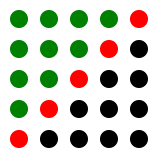
\includegraphics{/images/triangular_numbers_2.svg}
\end{figure}

Generalizing to arbitrary $n$, we have

\[n^2 = 2 \times T_{n-1} + n \rightarrow T_{n-1} = \frac{n^2 - n}{2} = \frac{n(n-1)}{2} \]

or

\[T_{n} = \frac{n(n+1)}{2}\]

This is a classic of counting the same arrangements in a different
(preferably simpler) way.

\subsubsection{Generating Functions}

Converting the sum $T_n \sum_{i=0}^n i$ into a recurrence relation, we obtain $T_n = T_{n-1} + n$; or equivalently

\[ T_{n+1} = T_n + (n+1); \qquad T_0 = 0\]

We can convert this into an expression for the generating function
$A(z)$ of $T_n$; namely

\[ \frac{A(z)-T_0}{z} = A(z) + \sum_{n \geq 0}n z^n + \sum_{n \geq 0} z^n \]

For the expression $\sum_{n \geq 0}n z^n$ we do the following: Consider the all-one series which generating function is $B(z) = \sum_{n \geq 0} 1 z^n = \frac{1}{1-z}$. We seek $n z^n$; this corresponds to $z B(z) = \frac{z}{(1-z)^2}$.

We therefore have

\[ \frac{A(z)-T_0}{z} = A(z) + \frac{z}{(1-z)^2} + \frac{1}{1-z} \rightarrow A(z) = \frac{z}{(1-z)^3}\]

A series expansion yields

\begin{verbatim}
      2     3      4      5      6      7      8      9
x + 3x  + 6x  + 10x  + 15x  + 21x  + 28x  + 36x  + 45x  + ...
\end{verbatim}

Another way would be to consider the sequence $1,2,3,4,\ldots$ with the generating function $A(z) = \sum_{n \geq 0} n z^n = \frac{z}{(1-z)^2}$. We want to obtain the sequence of the partial sums; the corresponding generating function is $\frac{A(z)}{1-z} = \frac{z}{(1-z)^3}$.

\subsubsection{Other Characteristics}

From the definition of the $T_n$, we have the following property:

\[ T_n + T_{n-1} = \frac{n(n+1)}{2} + \frac{n(n-1)}{2}  = n^2\]

and

\[ T_{n} - T_{n-1} = \frac{n(n+1)}{2} - \frac{n(n-1)}{2}  = n \]

Therefore, we have

\[ T_n + T_{n-1} = (T_{n} - T_{n-1})^2 \]

\subsection{Number of Line Segments}

Related to the triangular numbers are the numbers $L_n$ of direct connections between the objects; for example see the Figure below. For $n=4$ (red lines), we have $L_4 = 18$. Every node contributes
$3$ connections; therefore we have $L_n = 3 T_{n-1}$.


\todo{FIGURE}
\begin{figure}
\centering
%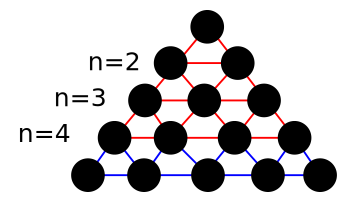
\includegraphics{/images/triangular_numbers_3.svg}
\end{figure}

A different argument leads to a recurrence relation for the $L_n$: If we have connections up to level $n$ ($n=4$) in the example above), then the next level adds another $3 \times n$ connections and we therefore have

\[ L_{n+1} = L_n + 3n\]

I.e. $L_5 = L_4 + 3 \times 4 = 18 + 12 = 30$.

\subsubsection{Generating Functions}

Just for the fun of it; we have

\[ \frac{A(z)}{z} = A(z) + 3 \sum_{n \geq 0} n z^n = A(z) + \frac{3z}{(1-z)^2} \rightarrow A(z) = \frac{3z^2}{(1-z)^3}\]

A series expansion yields

\begin{verbatim}
  2     3      4      5      6      7      8       9
3x  + 9x  + 18x  + 30x  + 45x  + 63x  + 84x  + 108x + ...
\end{verbatim}

%\DiaryEntry{2D Integral Substitution}{2015-10-27}{Integrals}

We want to solve a 2D-integral

\[ I = \int_x \int_y f(x,y) dy dx \]

and want to perform a substitution: $x = x(u, v); y = y(u; v)$. The integrand then becomes $f(u,v)$. In addition we need to transform the "$dx dy$-square" into its equivalent "$du dv$-square". This is
achieved by the Jacobian matrix which is defined as:

\[ J(u,v) = \left( \begin{array}{cc}
\frac{\partial x(u,v)}{\partial u} & \frac{\partial x(u,v)}{\partial v}  \\
\frac{\partial y(u,v)}{\partial u} & \frac{\partial y(u,v)}{\partial v} 
\end{array} \right) \]

Then the integral can be rewritten as

\[ I = \int_x \int_y f(x,y) dy dx = \int_u \int_v f(u,v) |J(u,v)| dv du \]

with $|J(u,v)|$ denoting the determinant of the Jacobian Matrix.

\subsubsection{Simple Example}

As a toy example, consider the integral which can be solved by
elementary means

\[ I = \int_{x=0}^1 \int_{y=0}^1 x y^2 dy dx = \frac{1}{6}\]

Making the substitution $u=x/2, v=3y$ leads to $x=2u, y=v/3$ and to the following Jacobian Matrix:

\[J(u,v) = \left( \begin{array}{cc} 2 & 0 \\ 0 & \frac{1}{3} \end{array} \right) \]

With the determinant being
$|J(u,v)| = \frac{2}{3}$, we arrive at (note the changed integration intervals!):

\[I = \int_{u=0}^{\frac{1}{2}} \int_{v=0}^3 2u \frac{v^2}{9} \frac{2}{3} dv du = \frac{1}{6}\]

\subsubsection{Solving the Integrals with SymPy}

... works as follows:

\begin{verbatim}
import sympy as sym
x, y = sym.symbols("x y")

res = sym.integrate(x*y**2, (x,0,1), (y,0,1))
sym.pprint(res)

res_subs = sym.integrate(2/3*2*x*y**2/9, (x,0,1/2), (y,0,3))
sym.pprint(res)
\end{verbatim}

\subsubsection{Polar Coordinates}

Consider the substitution from rectangular coordinates to polar
coordinates with the transformation rules $x = r \cos \phi; y = r \sin \phi $. The Jacobian therefore becomes

\[J(r, \phi) = \left( \begin{array}{cc} \frac{\partial x}{\partial r} & \frac{\partial x}{\partial \phi} \\ \frac{\partial y}{\partial r} & \frac{\partial y}{\partial \phi} \end{array} \right)
 = \left( \begin{array}{cc} \cos \phi & -r \sin \phi \\ \sin \phi & r \cos \phi \end{array} \right) \]

The determinant is $|J(r, \phi)| = r \cos^2 \phi + r \sin^2 \phi = r$ and therefore we have for the integral

\[ I = \int_x \int_y f(x,y) dy dx = \int_r \int_\phi f(r \cos\phi, r \sin\phi) r dr d\phi \]

%\DiaryEntry{Binomal Coefficients, Part I}{2015-10-28}{Combinatorics}

\subsection{Introduction}

A sequence (with non-repeating elements) depends on the order of its elements; whereas a set does not. The sequences $(1,2,3)$ and $(3,2,1)$ are therefore \textbf{different}; whereas the sets $\{1,2,3\}$ and $\{3,2,1\}$ are \textbf{equivalent}.

If we have a set of $n$ elements, we can generate $(n(n-1)\cdots(n-k+1)$) sequences of length $k$: There are $n$ possibilities for the first slot, $n-1$ possibilities for the second slot and so on. For the k-th slot (the last one), there are therefore $n-k+1$ possibilities left.

If we are interested in the number of sets, we need a relation between the number of different sequences and the number of different sets. A set with $k$ elements yields $k!$ different sequences. Therefore if we have a set of $n$ elements and we want to know how many sets of size $k$ we can build out of it, we have

\begin{equation}
\frac{n(n-1)\cdots(n-k+1)}{k!} = \frac{n!}{(n-k)!k!} = {n \choose k}
\end{equation}

possibilities.

\subsubsection{Example}

Consider the set $(\mathcal{S} =
\{1,2,3,4\}$) with $(n=4$)
and list all six 2-element subsets:

\[(1,2), (1,3), (1,4), (2,3), (2,4), (3,4)\]

We have ${4 \choose 2} = \frac{4 \cdot 3}{1 \cdot 2} = 6$. If we consider sequences instead, we have the following 2-element sequences:

\[(1,2), (1,3), (1,4), (2,1), (2,3), (2,4), (3,1), (3,2), (3,4), (4,1), (4,2), (4,3)\]

Note that e.g.~the sequences $(1,2)$) and $(2,1)$) are \textbf{not} equivalent and therefore counted separately. There are $(4 \cdot 3 = 12$) such subsequences. If we finally allow duplicate elements in the sequences, then we obtain the following

\[ (1,1), (1,2), (1,3), (1,4), (2,1), (2,2), (2,3), (2,4), (3,1), (3,2), (3,3), (3,4), (4,1), (4,2), (4,3), (4,4) \]

There are $n^k = 4^2 = 16$ such sequences.

\subsection{Identities}

Table of the binomial coefficients:

\begin{figure}[H]
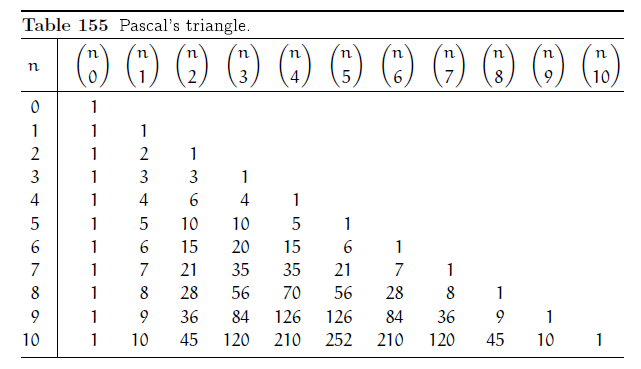
\includegraphics[scale=0.7]{images/binomials_01.png}
\end{figure}

We see that

\[ {n \choose 0} = 1, \quad {n \choose 1} = n, \quad  \quad {n \choose n} = 1 \]

From the definition of the binomial coefficients it can also be seen that ${n \choose 2} = \frac{n(n-1)}{2}$ and that the coefficients are symmetric. We have

\[ {n \choose n-k} = \frac{n!}{(n-(n-k))!(n-k)!} = \frac{n!}{k! (n-k)!} = {n \choose k} \]

This can be easily seen from the table above.

\subsubsection{Absorption Identity 1}

We have an absorption identity

\[ \frac{r}{k} {r-1 \choose k-1} = \frac{r}{k} \frac{(r-1)!}{(r-1-(k-1))!(k-1)!} = \frac{r}{k} \frac{(r-1)!}{(r-k)!(k-1)!} = \frac{r!}{(r-k)!k!} = {r \choose k} \]

which can be rewritten to

\begin{equation}
\label{eq:abs1}
r {r-1 \choose k-1} = k {r \choose k}
\end{equation}

\subsubsection{Absorption Identity 2}

Next we consider $(r-k) {r \choose k}$. By symmetry, we have $(r-k) {r \choose k } = (r-k) {r \choose r-k}$. Using \eqref{eq:abs1} (from right to left), we obtain

\[ (r-k) {r \choose k} = r {r-1 \choose r-k-1} \]

and using symmetry again,we arrive at

\[ (r-k) {r \choose k} = r {r-1 \choose r-1-(r-k-1)} = r {r-1 \choose k} \]

\subsection{Recurrence Relations}

A well-known recurrence relation is obtained by combining the identities from above:

\[ (r-k) {r \choose k} =  r {r-1 \choose k}, \quad k {r \choose k} = r {r-1 \choose k-1}\]

Summing the respective right and left sides yields

\[ (r-k) {r \choose k} + k {r \choose k} = r {r-1 \choose k} + r {r-1 \choose k-1}\]

Simplifying the left hand side and dividing the expression by $r$ yields the desired recurrence relation

\begin{equation}
\label{eq:recur}
{r \choose k} = {r-1 \choose k} + {r-1 \choose k-1}
\end{equation}

The coefficient in Pascal's triangle equals the coefficient one row above plus the coefficient one row above and on to the left.

The combinatorial interpretation is as follows: Consider a set of $n$ elements from which we want to select subsets of size $k$. There are ${n \choose k}$ ways to do this. Assume that one element (out of the $n$ is marked and therefore distinguishable from the other elements.

We can group the ${n\choose k}$ subsets into two sets: Set $\mathcal{S_u}$ contains all subsets without the marked element and set which includes the marked element.

The set $\mathcal{S_u}$ is generated by selecting subsets of size $k$ from the unmarked elements (there are $n-1$ of them). Therefore, this set contains ${n-1 \choose k}$ elements.

The set $\mathcal{S_m}$ is generated by selecting subsets of size $k$ which contain the marked element. Since the marked element is included, there are $n-1$ remaining elements to choose from and these are placed into subsets of size $k-1$. Therefore, this set contains ${n-1 \choose k-1}$) subsets.

These two cases (marked element included and not included) cover all possibilities, therefore above relation holds.

This recurrences can also be shown by elementary operations of the binomial coefficient definition. The RHS of \eqref{eq:recur} is

\begin{align*}
{r-1 \choose k} + {r-1 \choose k-1} &= \frac{(r-1)!}{(r-1-k)!k!} + \frac{(r-1)!}{(r-1-(k-1))!(k-1)!} \\&= \frac{(r-1)!}{(r-1-k)!k!} + \frac{(r-1)!}{(r-k)!(k-1)!}
\end{align*}

Making a common denominator we obtain

\begin{align*}
{r-1 \choose k} + {r-1 \choose k-1} &= \frac{(r-1)! (r-k)}{(r-1-k)!k!(r-k)} + \frac{(r-1)!k}{(r-k)!(k-1)!k} \\&= \frac{(r-1)! (r-k)}{(r-k)!k!} + \frac{(r-1)!k}{(r-k)!k!} = \frac{(r-1)! r}{(r-k)!k!}
\end{align*}

and finally we obtain

\[
{r-1 \choose k} + {r-1 \choose k-1} = \frac{r!}{(r-k)!k!} = {r \choose k}
\]

\subsubsection{Example}

Considering the example from above with $\mathcal{S} = \{1,2,3,4\}$ and $k=2$, we have

\[{4 \choose 2} = {3 \choose 2} + {3 \choose 1} = 3 + 3 = 6\]

If we choose 1 as the ``marked'' element, we can split $\mathcal{S}$ into the set $\mathcal{S_m}$ containing 1 and the set $\mathcal{S_u}$ not containing 1 as follows:

\[ \mathcal{S_m} = {(1,2), (1,3), (1,4)}, \quad  \mathcal{S_u} = {(2,3), (2,4), (3,4)} \]

\subsection{Binomial Theorem}

The binomial theorem states that

\[ (x+y)^r = \sum_k {r \choose k} x^k y^{r-k} \]

Note that this identity holds for \emph{any} (real) number $r$. In the special case of $r$ being an integer, the expression simplifies to

\[ (x+y)^r = \sum_{k=0}^r {r \choose k} x^k y^{r-k} \]

The special case $y = 1$ yields

\[ (1+x)^r = \sum_k {r \choose k} x^k \]

By choosing $x=1$, we obtain

\[ \sum_{k=0}^r {r \choose k} = 2^r \]

I.e. the sum of the r-th row in Pascal's triangle equals $2^r$. The combinatorial interpretation is as follows: Consider binary sequences of length $n$. There are ${n
\choose 0}$ sequences which contain $0$ zeros, there are ${n \choose 1}$ sequences which contain $1$ zero, and so on. Finally, there are ${n \choose n}$ sequences which contain $n$ zeros. This enumeration contains all binary sequences of length n which equals $2^n$.

By choosing $x=-1$, we obtain

\[ \sum_{k=0}^r {r \choose k} (-1)^k = 0 \]

I.e. the alternating sum of any row in Pascal's triangle equals zero.

When we expand \((1-x)^n\) we obtain

\[
(1-x)^n = \sum_k {n \choose k} (-1)^k x^k
\]

Differentiating both sides with respect to \(x\) yields:

\[
(-1)n(1-x)^{n-1} = \sum_k {n \choose k} (-1)^k k x^{k-1}
\]

and setting \(x=1\) we obtain the relation

\[
\sum_k (-1)^k k {n \choose k} = 0
\]

%\DiaryEntry{Rising and Falling Factorials}{2015-10-29}{Combinatorics}

\subsection{Definition}

Falling factorial: $x^{\underline{n}} = x(x-1)\cdots(x-n+1)$ and rising factorial $x^{\overline{n}} = x(x+1)\cdots(x+n-1)$.

\subsubsection{Identities}

We have

\begin{equation}
\label{eq:iden}
x^{\underline{n+1}} = x^{\underline{n}} (x-n), \qquad x^{\overline{n+1}} = x^{\overline{n}} (x+n)
\end{equation}

The connection between falling and rising polynomials is as follows

\begin{equation}
x^{\underline{n}} = (-1)^n (-x)^{\overline{n}}
\end{equation}

We can prove this via induction; assume the identity holds for $n$ and show that it holds for $n+1$:

\[x^{\underline{n+1}} = (-1)^{n+1} (-x)^{\overline{n+1}}\]

Expansion of both sides by using \eqref{eq:iden} yields

\[x^{\underline{n}}(x-n) = (-1)^{n+1} (-x)^{\overline{n}}(-x+n)\]

Inserting the induction basis (for $n$) on the LHS for $x^{\underline{n}}$, we arrive at

\[ (-1)^n (-x)^{\overline{n}} (x-n) = (-1)^{n+1} (-x)^{\overline{n}}(-x+n)\]

Canceling terms on both sides yields

\[ x-n = (-1)(-x+n) \quad \star\]

\subsection{Difference Operator}

We define a difference operation of a sequence $f(n)$ as

\begin{equation}
\Delta f(n) = f(n+1) - f(n)
\end{equation}

For falling factorials, the difference operation becomes

\[
\Delta x^{\underline{n}} = (x+1) \color{red}{ x(x-1)\cdots(x-n+2)} - \color{red}{x(x-1)\cdots(x-n+2)} (x-n+1)
\]

The red part appears in both parts of the difference and can be factor out, resulting in the simple expression for the difference operation:

\begin{align*}
\Delta x^{\underline{n}} &= x(x-1)\cdots(x-n+2) \big[ (x+1) - (x-n+1) \big] \\
&= n x(x-1)\cdots(x-n+2) = n x^{\underline{n-1}}
\end{align*}


\subsubsection{Usage in Sums}

Similar to the Fundamental Theorem of Calculus, we have a theorem for finite differences. If $g(x) = \Delta f(x)$, then

\begin{equation}
\label{eq:fund}
\sum_{a \leq x < b} g(x) = f(b) - f(a)
\end{equation}

This can be proven as follows: Insert the definition of the difference operation into \eqref{eq:fund} to obtain

\begin{align*}
\sum_{a \leq x < b} g(x) &= \sum_{a \leq x < b} \big( f(x+1) - f(x) \big) \\
&= f(a+1) - f(a) + f(a+2) - f(a+1) + \cdots \\ 
& + f(b) - f(b-1) + f(b-1) - f(b-2)
\end{align*}

This is a telescoping sum and all terms but two cancel. Therefore, we have

\[
\sum_{a \leq x < b} g(x) = f(b) - f(a)
\]

When summing expressions with the difference operator, we have

\[
\sum_{0 \leq x < N} x^{\underline{n}} = \frac{x^{\underline{n+1}}}{n+1} \bigg|_0^N = \frac{N^{\underline{n+1}}}{n+1}
\]

\subsubsection{Example}

Take $f(x) = x^{\underline{2}}=x(x-1)$ and $g(x) = \Delta x^{\underline{2}} = 2 x^{\underline{1}} = 2x$. Then we have

\[
\sum_{a \leq x < b} g(x) = \sum_{a \leq x < b} 2x = f(b) - f(a) = b(b-1) - a(a-1)
\]

This is correct, because $\sum_{0 \leq x < N} 2x = 2 \frac{N(N-1)}{2} = N(N-1)$.

We can sum ordinary powers when we express them in terms of falling factorials. For example, we have $x^2 = x^{\underline{2}} + x^{\underline{1}}$ and therefore,

\[
\sum_{0 \leq x < N} x^2 = \sum_{0 \leq x < N} x^{\underline{2}} + x^{\underline{1}} = \frac{N^{\underline{3}}}{3} + \frac{N^{\underline{2}}}{2} = \frac{1}{2} N (N-1/2)(N-1)
\]

\subsection{Stirling Numbers, 2nd Kind}

The connection between ordinary powers and falling factorials is given by Stirling Numbers of the 2nd kind ${n \brace k}$. They count the number of ways to partition a set of $n$ things into $k$ nonempty subsets.

For example, there are seven ways to split a four-element set into two parts (${4 \brace 2} = 7$):

\[
\{1,2,3\} \cup \{4\}, \{1,2,4\} \cup \{3\}, \{1,3,4\} \cup \{2\}, \{2,3,4\} \cup \{1\}, \{1,2\} \cup \{3,4\}, \{1,3\} \cup \{2,4\}, \{1,4\} \cup \{2,3\}
\]

If we want to partition a set with $n$ elements into $k$ subsets, we can (i) put a marked element into its own subset. There are ${n-1 \brace k-1}$ ways to do this. Or (ii), we put it with other elements in a subset. There are $k {n-1 \brace k}$ ways to do this: There are $n-1$ elements remaining and these will be placed into $k$ subsets
- that is ${n-1 \brace k}$ ways and there are $k$ subsets for the marked element to join. We therefore have

\begin{equation}
{n \brace k} = {n-1 \brace k-1} + k {n-1 \brace k}
\end{equation}

The following table shows the Stirling Numbers fro some $n$ and $k$.

\begin{figure}[H]
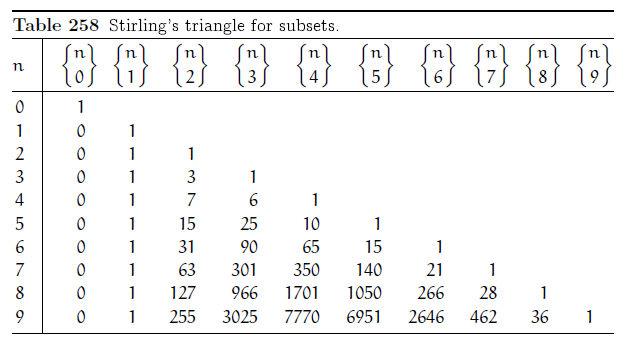
\includegraphics[scale=0.7]{images/stirling_2nd.png}
\caption{Page1}
\end{figure}

An ordinary power can then be expressed in terms of falling factorials as follows

\begin{equation}
x^n = \sum_k {n \brace k} x^{\underline{n}}
\end{equation}

%\DiaryEntry{Nonlinear Dynamics and Chaos, 1}{2015-11-01}{Maths}

Based on the book ``Nonlinear Dynamics and Chaos'' from Strogatz.

\subsection{One-dimensional Flows}

Consider a (one-dimensional) function $x(t)$ and we are given its derivative (with respect to t) in terms of a function $f(x)$. Note that $f(x)$ does \emph{not} depend on the time parameter $t$:

\[
\frac{dx(t)}{dt} = f(x)
\]

There may only be a numerical solution to this differential equation; however, the expression provides insights into the solution(s). Upon drawing the relation between $x$ and $\frac{dx(t)}{dt}$, we can find intervals of $x$, where the derivative is (i) positive and therefore $x(t)$ will increase, (ii) is negative and therefore $x(t)$ will decrease, and (iii) is zero and therefore $x(t)$ will stay constant (if $\frac{dx(t)}{dt} = 0$ for $x=x^\star$, then $x(t)=x^\star$). The latter points / regions are called fixed points.

\subsubsection{Stability of Fixed Points}

Assume $x^\star$ is a fixed point. If $\frac{dx(t)}{dt} < 0$ for $x > x^\star$, then $x(t)$ will increase. Similarly, if $\frac{dx(t)}{dt} > 0$ for $x < x^\star$, then $x(t)$ will decrease. In short, if $x$ deviates from the fixed point, the derivative will ``pull'' it back towards the fixed point $x^\star$. Such a fixed point is called a stable fixed point. The condition on the behavior of $\frac{dx(t)}{dt}$ around the fixed point is equivalent to a negative slope of $\frac{dx(t)}{dt}$.

Conversely, if the derivative ``pushes'' away from the fixed point ($\frac{dx(t)}{dt} > 0$ for $x > x^\star$ and $\frac{dx(t)}{dt} < 0$ for $x < x^\star$), the fixed point is called an unstable one. This is equivalent to a positive slope of $\frac{dx(t)}{dt}$.

This can be seen as a one-dimensional vector field on the x-axis; the
direction and length of the vectors are given by $f(x)$. The Figure below shows an example of a system with one stable fixed point $x_1$ (the slope is negative) and an unstable fixed point $x_2$ (the slope
is positive).

\begin{figure}[H]
\centering
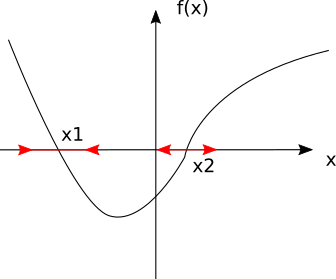
\includegraphics{images/strogatz_1_1.png}
\caption{Page1}
\end{figure}

In a one-dimensional system, the solutions $x(t)$ either approach a fixed point or diverge to $\pm \infty$. No oscillations are possible.


\subsubsection{Example}

We have

\[
\frac{df}{dx} = \sin(x)
\]

Fixed points are at location $x^\star = k \pi$ with stable fixed points at odd $k$ (here the slope is negative) and unstable fixed points at even $k$ (the slope being positive).

\subsection{Two-dimensional Flows}

Here we have two functions $x=x(t), y=y(t)$ with system equations as follows:


\begin{align*}
\frac{dx}{dt} & = f(x,y) \\
\frac{dy}{dt} & = g(x,y)
\end{align*}


In order to visualize what is going on, we use phase plane which is a
two- dimensional vector field with components $(f(x,y), g(x,y))^T$. The trajectories of the phase plane describe possible solutions: An actual solution starts at some initial value $(x\_0, y\_0)$ and then moves along the trajectory. The norm of the vector $(f(x,y), g(x,y))^T$ can be interpreted as the speed with which the vector field is traversed.

With this interpretation, a norm of zero implies no movement along the trajectory; in other words, the solution has arrived at a fixed point. The norm of a vector becomes only zero when all components vanish. Therefore, a fixed point is a point $(x^\star,y^\star)$ for which $f(x^\star, y^\star) = g(x^\star,y^\star) = 0$.

Depending on the starting point, the trajectory may end up in a fixed
point, diverge, or oscillate in the phase plane.

There is a result that such systems of differential equations always
have a unique solution (which may depend on initial values). Therefore, trajectories will never intersect. If there would be an intersection, then two solutions would start from the same point (the intersection) which would violate the uniqueness constraint.

An immediate consequence is, that if there is a closed trajectory
$\mathcal{C}$ in the phase plane, it separates the trajectories into an ``inside'' and ``outside''. The ``inside'' trajectories cannot cross $\mathcal{C}$ and get ``outside''; vice versa for the ``outside trajectories'' which cannot get ``inside''.


\subsubsection{Stability of Fixed Points}

To analyze fixed points, the Jacobian matrix of the system is used. The Jacobian is defined as

\[ J(x,y) = \left( \begin{array}{cc}
\frac{\partial f(x,y)}{\partial x} & \frac{\partial f(x,y)}{\partial y}  \\
\frac{\partial g(x,y)}{\partial x} & \frac{\partial g(x,y)}{\partial y}
\end{array} \right) \]

Based on the values of the Jacobian eigenvalues, the following
distinction is made:

\begin{itemize}
\item
  If both eigenvalues have positive real part, the fixed point is an
  unstable point and repels trajectories.
\item
  If both eigenvalues have negative real part, the fixed point is a
  stable point and attracts trajectories.
\item
  If one eigenvalue is positive and the other negative, the fixed point   is a saddle point.
\item
  If both eigenvalues are imaginary, one or both eigenvalues are zero, the fixed point is a center / higher order point.
\end{itemize}

If there are several stable fixed points in a system, the $x-y$-space can be separated into several basins: All initial points $(x_0, y_0)$ which eventually ($t \rightarrow \infty$) end up in the same fixed point belong into the same basin.


\subsubsection{Example}

Consider the following system

\begin{align*}
\frac{dx}{dt} & = x(3-x-2y) \\
\frac{dy}{dt} & = y(2-x-y)
\end{align*}

Setting the LHS to zero in both equations, we get 4 fixed points:
$(0,0), (0,2), (3,0), (1,1$.

The Jacobian has the following form

\bee
J(x,y) = \left(
\begin{bmatrix}{cc}
3-2x-2y & -2x  \\
-y & 2-x-2y  
\end{bmatrix}
\right)
\eee

In the following we will calculate the Jacobi matrix for the 4 fixed
points and analyze the Jacobian's eigenvalues.

\begin{itemize}
\item
  Fixed point $(0,0)$: The Jacobian becomes \[J(x,y) = \left(
  \begin{array}{cc} 3 & 0  \\ 0 & 2 \end{array} \right) \] with
  eigenvalues 3 and 2. They are positive, therefore the fixed point is a repelling one.
\item
  Fixed point $(0,2)$: The Jacobian becomes \[J(x,y) = \left(
  \begin{array}{cc} -1 & 0  \\ -2 & -2 \end{array} \right) \] with two negative eigenvalues (-1 and -2). Therefore the fixed point is an attracting one.
\item
  Fixed point $(3,0)$: The Jacobian becomes \[J(x,y) = \left(
  \begin{array}{cc} -3 & -6  \\ 0 & -1 \end{array} \right) \] with two   negative eigenvalues (-1 and -3). Therefore the fixed point is an attracting one.
\item
  Fixed point $(1,1)$: The Jacobian becomes \[J(x,y) = \left(
  \begin{array}{cc} -1 & -2  \\ -1 & -1 \end{array} \right) \] with one   negative and one positive eigenvalue ($-1 \pm \sqrt{2}$). Therefore the fixed point is a saddle point.
\end{itemize}

The Figure below shows the (numerically obtained) phase portrait which supports the calculations together with the 4 fixed points.

\begin{figure}[H]
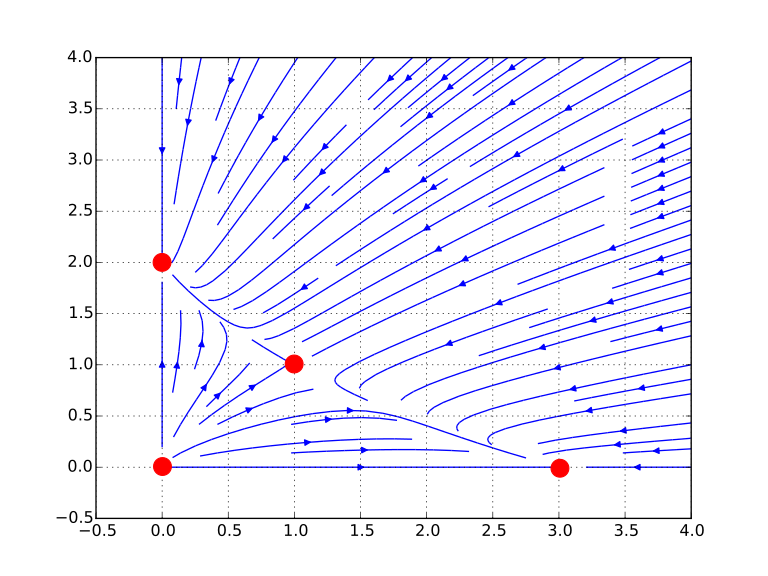
\includegraphics[scale=0.7]{images/strogatz_1_2.png}
\end{figure}

The Figure below shows the example trajectory starting at $(3,3)$ being ``swallowed'' by the fixed point $(0,2)$.

\begin{figure}[H]
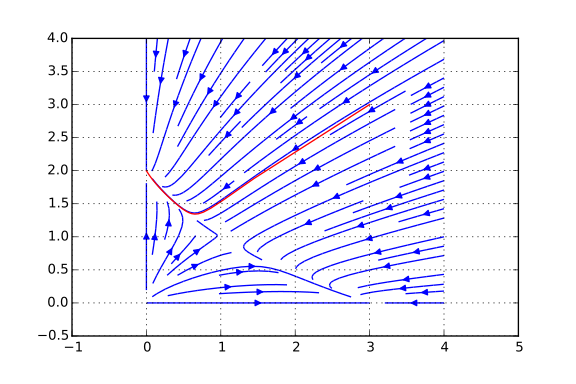
\includegraphics[scale=0.7]{images/strogatz_1_3.png}
\end{figure}

The corresponding plots of $x(t)$ and $y(t)$ as functions of
$t$ have the following form

\begin{figure}[H]
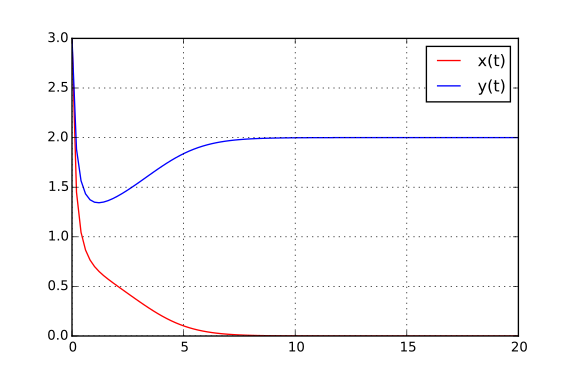
\includegraphics[scale=0.7]{images/strogatz_1_4.png}
\end{figure}

The function $y(t)$ makes a ``dip'' to $\approx 1.4$ before it converges to $2$. $x(t)$ converges to zero with ``two velocities''; before the ``dip'' the rate of decrease is larger than afterwards.

%\DiaryEntry{Nonlinear Dynamics and Chaos, 2}{2015-11-01}{Maths}

\subsubsection{Conservative System}

Based on Newton's law that $F=ma$. If a particle moves alone the x-axis and is subject to a non-linear force $F(x)$, we have

\[m \frac{d^2x(t)}{dt^2} = F(x)\]

Note the independence of $F(x)$ on both the derivative of $x(t)$ and the time $t$ itself.

If $V(x)$ denotes the potential energy $F(x) = - dV(x)/dx$, we have

\[m \frac{d^2x(t)}{dt^2} + \frac{dV(x)}{dx} = 0\]

If we multiply both sides of the equation with $dx(t)/dt$, we obtain

\[m \frac{dx(t)}{dt} \frac{d^2 x(t)}{dt^2} + \frac{dx(t)}{dt} \frac{dV(x)}{dx} = 0\]

The left part can be rewritten as

\[
\frac{d}{dt} \left[ \frac{1}{2} m \left(\frac{dx(t)}{dt}\right)^2 \right] = \frac{1}{2} m \frac{d^2 x(t)}{dt^2} 2 \frac{dx(t)}{dt} = m \frac{dx(t)}{dt} \frac{d^2 x(t)}{dt^2}
\]

the right part is (inverse chain rule)

\[
\frac{dx(t)}{dt} \frac{dV(x)}{dx} = \frac{dV(x)}{dt}
\]

We therefore have

\[
\frac{d}{dt} \left( \frac{1}{2} m \left(\frac{dx(t)}{dt}\right)^2 + V(x) \right) = 0
\]

This means that the total energy $E = \frac{1}{2} x'^2 + V(x)$ is constant for any solution of the system. In other words, the energy $E$ stays constant along trajectories.

\subsubsection{Limit Cycles}

A limit cycle is an isolated closed trajectory. Isolated means that nearby trajectories are not closed and spiral either toward (stable limit cycles) or away from the limit cycle (instable limit cycles). An example of a stable limit cycle and an unstable limit cycle are shown below.

\begin{figure}[H]
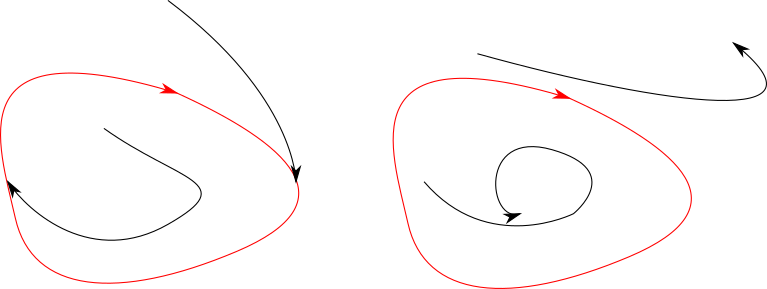
\includegraphics[scale=0.7]{images/strogatz_2_1.png}
\end{figure}

\subsection{Poincaré-Bendixon Theorem}

If

\begin{itemize}
\item
  R is a closed bounded subset of a plane
\item
  the system is continuously differentiable on R
\item
  R does not contain any fixed points
\item
  there is a trajectory C confined to R (i.e.~it stays within R for from $t=0$ till $t \rightarrow \infty$),
\end{itemize}

then C is a closed orbit or it spirals towards a closed orbit as
$t \rightarrow \infty$. In any case, R contains a closed orbit.

We can interpret the theorem that the dynamical possibilities of \textbf{two- dimensional} systems are limited. If a trajectory is confined to a closed, bounded region without fixed points, it must eventually approach a closed orbit. In higher-order dimensions, the theorem does not hold; therefore chaos (more ``dynamic'' behavior is
possible).

%\DiaryEntry{Memoryless Property}{2015-11-17}{Stochastic}

Based on the entry random processes from 2015-08-30, a \textbf{non- negative} RV $X$ is defined memory-less, if

\[ P(X>t+s|X>t) = P(X>s)\]

for $s, t$ positive. The interpretation of this property is: When $X$ has made it beyond $t$, the random variable is ``started anew''.

Note that the events $X>t$ and $X>s$ are not independent; if they were, we would have the following property

\[ P(X>s|X>t) = P(X>s)\]

The only continuous distribution which fulfills the memoryless property is the exponential distribution.

\subsubsection{Uniform Distribution}

As a counter-example we consider the uniform distribution on
${[}0;1{]}$.

\begin{figure}[H]

\includegraphics[scale=0.7]{images/memory_less_1.png}
\end{figure}

Next we obtain

\[ P(X>t+s|X>t) = \frac{P(X>t+s, X>t)}{P(X>t)} = \frac{P(X>t+s)}{P(X>t)} \]

where in the last step we used the fact that $s$ and $t$ are positive (if $X$ is bigger than $t+s$, it is also bigger than $t$).

We seek an expression as function of $s$, parametrized by $t$. Fix $t=1/2$ and we have

\[ f(s; t=1/2) = P(X>s+1/2|X>t) = \frac{P(X>s+1/2)}{1/2} \]

For $s=0$, we have $f(s=0; t=1/2)=1$ and for $s=1/2$, we have $f(s=1/2; t=1/2)=0$. With the help of wolfram alpha, we can fill in the missing points (also for other values of $t$ and the distributions $P(X>t+s|X>t)$ have the following form:

\begin{figure}[H]

\includegraphics[scale=0.7]{images/memory_less_2.png}
\end{figure}

Comparing with the upper right Figure, we see that $P(X>t+s | X>t)
\neq P(X>s)$; the uniform distribution is not memoryless.

\subsubsection{Exponential Distribution}

should be memoryless, but sympy does not allow for this... to be
continued :-(

%\DiaryEntry{Cauchy Inequality - Application}{2015-11-23}{Maths}

\subsubsection{Inner Product}

We can interpret the \(a_k\) as elements of a vector. In this case, all inequalities extend to the vector case; for example, the Cauchy
inequality becomes

\[
<\mathbf{a},\mathbf{b}> \leq |\mathbf{a}|^2 |\mathbf{b}|^2
\]

where \(\mathbf{a}\) denotes a vector and \(<\mathbf{a},\mathbf{b}>\)
denotes the inner product between two vectors \(\mathbf{a}\) and
\(\mathbf{b}\)

The second inequality becomes

\[
<\mathbf{a},\mathbf{b}> \leq \frac{1}{2} |\mathbf{a}|^2 + \frac{1}{2} |\mathbf{b}|^2
\]

\subsubsection{Bound on \(\sum 1/k\)}

Set the sequence $b_n=1$ (for all $n$), and we obtain the following inequality

\[ \sum_k a_k \leq \sqrt{N} \sqrt{\sum_k a_k^2} \]

As a simple example consider $a\_n = \frac{1}{n}$ and we have

\[ \sum_k \frac{1}{k} \leq \sqrt{N} \sqrt{\frac{\pi^2}{6}} \]

Note that the RHS divergers, but this does \textbf{not} imply that also the LHS diverges. There could well be another expression
$X$ which is smaller than the RHS, but which converges. Existence of this $X$ would then allow to deduce the convergence of the LHS.

\subsubsection{Splitting}

If we have a sum $\sum_k a_k $ we can split the summand $a_k$ as follows: $a\_k = |a_k|^{1/3} |a_k|^{2/3}$. Applying Cauchy's
inequality to this sum, we have

\[
\sum_k a_k = \sum_k |a_k|^{1/3} |a_k|^{2/3} \leq \left( \sum_k |a_k|^{2/3} \right)^{1/2} \left( \sum_k |a_k|^{4/3} \right)^{1/2}
\]

%\DiaryEntry{Convex Optimization, 1}{2015-12-07}{Optimization}

\subsection{Convex Sets}

Consider two points $P\_1, P\_2$ in an n-dimensional space $\mathcal{R}^n$. A line $l(\theta)$ connecting these two points is given by

\[
l(\theta) = \theta P_1 + (1-\theta) P_2, \quad \theta \in [0,1]
\]

If $\theta=1$, we are at $P_1$, for $\theta=0$, we are at $P_2$. For all values of $\theta$ in $[0,1]$, we are somewhere in between the two points.

A set $\mathcal{C}$ is called convex, if for any two points $P_1, P_2
\in \mathcal{C}$, the line connecting these two points is also in $\mathcal{C}$; i.e. $l(\theta) \in \mathcal{C}$ for $\theta$ in $[0,1]$.

\subsubsection{Hyperplanes}

A hyperplane is given by the set

\[ \{ x | a^T (x - x_0) = 0 \} \]

where $x, a, x_0$ are all n-dimensional vectors; $x_0$ being the displacement of the hyperplane from the origin and $a$ denoting the normal vector of the plane.

\paragraph{Two-dimensional Example}

In this case $x = (x , y)^T$, $a = (a_1 , a_2)^T$, $x_0 = (x_0 , y_0)^T$ and we have

\[
a_1(x - x_0) + a_2(y - y_0) = 0 \rightarrow y = \frac{a_1 x_0 + a_2 y_0}{a_2} - \frac{a_1}{a_2}x
\]

If $a = (1 , 1)^T$ and $x_0 = (1 , 0)^T$, we have $y = 1-x$.

\subsubsection{Halfspaces}

A halfspace is the area ``below'' a hyperplane; i.e.~the set

\[ \{ x | a^T (x - x_0) \leq 0 \} \]

\begin{figure}[H]
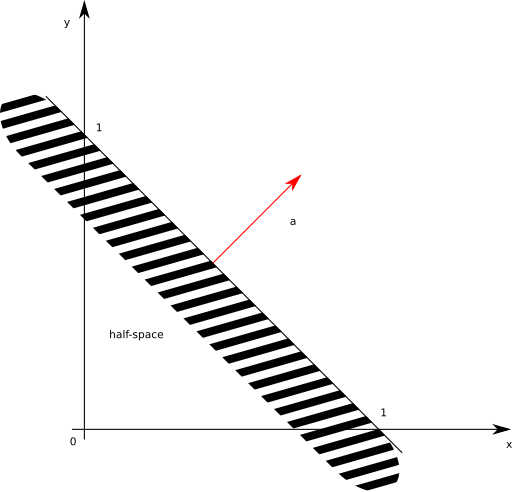
\includegraphics[scale=0.7]{images/convex_opt_01.png}
\end{figure}

A halfspace is always a convex set.

\subsubsection{Polyhedra}

Polyhedras $\mathcal{P}$ are combinations of halfspaces; i.e.

\[
\mathcal{P} = \{ x | A x \leq b, Cx = d  \}
\]

$A, C$ are matrices, $b, d$ are vectors.

\subsection{Convex Functions}

A convex function $f(x)$ is characterised by

\[
f(\theta x + (1-\theta)y) \leq \theta f(x) + (1-\theta)f(y)
\]

We can interpret the LHS a inputing any point on the line between
$x, y$ into the function. Then the function must be below (or equal) the line connecting the points $x, f(x)$ and $y, f(y)$ (the RHS).

\begin{figure}[H]
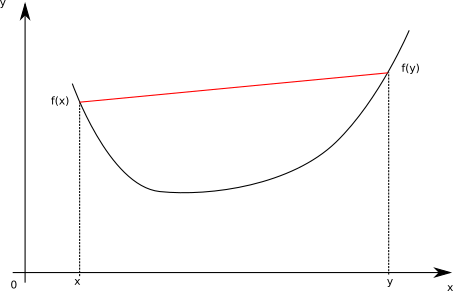
\includegraphics[scale=0.7]{images/convex_opt_02.png}
\end{figure}

An equivalent condition is

\[
f(y) \geq f(x) + \nabla f(x)^T (y-x)
\]

where the RHS is the tangent to $f(x)$ at point $(x, f(x))$.

And another equivalent condition is that

\[
\nabla^2 f(x) \geq 0
\]

i.e.~the second derivative (matrix) is positive (semi-definite).

\subsubsection{Basic Convexity Conditions}

There are some basic rules about convex functions:

\begin{itemize}
\item
  Linear and affine functions are convex
\item
  Quadratic functions $f(x) = 1/2 x^T P x + q^T x + r$ are convex if $\nabla^2 f(x) = P $ is positive semidefinite.
\item
  The function $e^{a x}$ is convex
\item
  The function $|x|^p, p \geq 1$ is convex
\item
  The functions $\log(x)$ and $x \log(x)$ are convex
\item
  Every norm is convex: Every norm $|x|$ (in order to
  be a norm) fulfills the triangle inequality:
  $|x+y| \leq |x| + |y|$. This can be stated differently in that we write
\end{itemize}

\[
\|\theta x+(1-\theta) y\| \leq \|\theta x\| + \|(1-\theta) y\| = \theta \|x\| + (1-\theta) \|y\|
\]

Sublevel sets of convex functions are convex sets: An $\alpha-$sublevel $C_\alpha$ of a function is defined as $C_\alpha = \{ x | f(x) \leq \alpha \}$. Assume that $x,y \in C_\alpha$, then we have $f(x), f(y) \leq \alpha$. We have

\[
f(\theta x + (1-\theta)y) \leq \theta f(x) + (1-\theta) f(y) \leq \theta \alpha + (1-theta) \alpha = \alpha
\]

where the first inequality follows from convexity of $f$ and the second inequality follows because of $x,y \in C_\alpha$.

\subsubsection{Convexity-preserving Operations}

\begin{itemize}
\item
  A non-negative weighted sum $f(x) = w_1 f_1(x) + w_2 f_2(x) + \cdots $ of convex functions is convex.
\item
  An affine mapping of a convex functions parameter is convex
  $f(Ax + b)$
\item
  The point-wise maximum of functions $f(x) = \max(f_1(x), f_2(x), \ldots )$ is convex.
\end{itemize}

We have

\[
f(\theta x + (1-\theta)y) = \max\{ f_1( \theta x + (1-\theta)y ) , f_2( \theta x + (1-\theta)y ) \} \leq \max \{ \theta f_1(x) + (1-\theta)f_1(y), \theta f_2(x) + (1-\theta)f_2(y) \} 
\]

using convexity. Now comes an interesting trick; we have

\[
\leq \theta \max \{ f_1(x), f_2(x)\} + (1-\theta) \max \{ f_1(y), f_2(y) \} = \theta f(x) + (1-\theta) f(y)
\]

%\DiaryEntry{Convex Optimization, 2}{2015-12-07}{Optimization}

\subsection{Convex Optimization}

The generic (convex) optimization problem has the following form:


\begin{align*}
p^\star & = \min f(x) \\
f_i(x) & \leq 0 \, (i=1 \ldots m) \\
h_i(x) & = 0 \, (i=1 \ldots p) \\
\end{align*}


Points $x$ fulfilling these conditions are called feasible points; the set of all feasible points is the feasible set.

\subsection{Lagrangian Function}

We define the Lagrangian function as

\[
L(x,\lambda,\nu) = f(x) + \sum_i \lambda_i f_i(x) + \sum_i \nu_i h_i(x)
\]

The dual function of the optimization problem is

\[
g(\lambda, \nu) = \inf_x L(x,\lambda,\nu)
\]

Being a point-wise infinum of affine functions, the dual function is \textbf{always} concave, even if the original problem is not convex. The dual function yields a lower bound on $p^\star$; for $\lambda \geq 0 $ and any feasible point $\tilde x$ (therefore $f_i(\tilde x) < 0$ and $h_i(\tilde x)=0$) we have

\[
\sum_i \lambda_i f_i(\tilde x) + \sum_i \nu_i h_i(\tilde x) \leq 0
\]

Therefore

\[
g(\lambda, \nu) = \inf_x L(x,\lambda,\nu) \leq L(\tilde x, \lambda, \nu) \leq f(\tilde x)
\]

\subsubsection{Lagrange Dual Problem}

For $\lambda \geq 0$, the Lagrange dual gives a lower bound on the optimal value $p^\star$. This bound depends on $\lambda$ and $\nu$ and we can therefore ask for the optimal lower bound:


\begin{align*}
d^\star = \max & \, g(\lambda, \nu) \\
\text{s.t.} \lambda & \geq 0
\end{align*}


This is the Lagrange dual problem associated with the original optimization problem. The solution, the values $(\lambda^\star, \nu^\star)$, are the dual optimal or optimal Lagrange multipliers. We have $d^\star \leq p\star $; i.e.~the solution of the dual problem is less or equal the solution of the original optimization problem. The difference between these two, $p^\star - d^\star $, is called the duality gap. In case of weak duality, the duality gap is strictly larger than zero; in case of strong duality, we have $d^\star = p^\star $.

\subsection{Optimality Conditions (KKT Conditions)}

If $f_i$ are convex and $h_i$ are affine, then any points $\tilde x, \tilde \lambda, \tilde \nu$ satisfying


\begin{align}
\label{kkt1} f_i(\tilde x) & \leq 0 \\
\label{kkt2} g_i(\tilde x) & = 0 \\
\label{kkt3} \tilde \lambda_i & \geq 0 \\
\label{kkt4} \tilde \lambda_i f_i(\tilde x) & = 0 \\
\label{kkt5} \nabla f(\tilde x) + \sum_i \tilde \lambda_i \nabla f_i(\tilde x) + \sum_i \tilde \nu_i \nabla h_i(\tilde x) & = 0
\end{align}


are primal / dual optimal (with zero duality gap). Equations
$\eqref{kkt1}$ and $\eqref{kkt2}$ ensure that $\tilde x$ is feasible. $\eqref{kkt3}$ ensures that the Lagrangian is convex (in x); and $\eqref{kkt5}$ ensures that $\tilde x$ minimizes the Lagrangian over $x$.

\subsubsection{Example 1}

Consider the problem


\begin{align*}
\min f(x) &= x^2 \\
\text{s.t.} \, x-2 & \leq 0
\end{align*}


The Lagrangian becomes $L(x,\lambda) = x^2 + \lambda (x-2)$

The following figure shows the objective function (in red) and the
Lagrangian for increasing values of $\lambda$ (in blue). In the feasible region ( i.e.~for $x\leq 2$), the Lagrangian underestimates the objective function.

\begin{figure}[H]
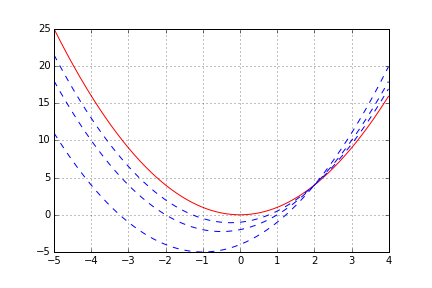
\includegraphics[scale=0.7]{images/convex_opt_03.png}
\end{figure}

The dual function is

\[
g(\lambda) = \inf_x L(x, \lambda) = \inf_x \big\{ x^2 + \lambda (x-2) \big\}
\]

Setting the derivative of $L$ with respect to $x$ to zero yields, $x=-\lambda/2$. Therefore, we have

\[
g(\lambda) = \left(-\frac{\lambda}{2}\right)^2 + \lambda \left( -\frac{\lambda}{2} - 2 \right) = - \frac{\lambda^2}{4} - 2\lambda
\]

The following plot shows the dual function $g(\lambda)$. Solving the dual problem $\eqref{dual}$; i.e.~maximizing $g(\lambda)$ with the constraint $\lambda > 0$ we see that the solution is $\lambda^\star = 0$ (yielding $d^\star = g(\lambda^\star)=0$).

\begin{figure}[H]
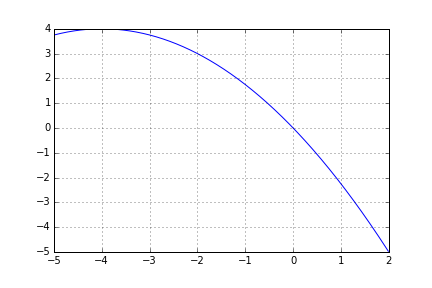
\includegraphics[scale=0.7]{images/convex_opt_03a.png}
\end{figure}

Using the KKT condition $\eqref{kkt5}$,

\[
\frac{dL}{dx} = 2x + \lambda = 0 \rightarrow x = - \frac{\lambda}{2}
\]

and the KKT condition $\eqref{kkt4}$ yields $\lambda(x-2) = 0$. From this last condition, we see two possible solutions: (A) $\lambda = 0 $ and (B) $x=2$. Starting with (A), it follows that $x=0$; for option (B) we have $\lambda=-4$. From $\eqref{kkt3}$ this is not allowed, therefore the (only) solution to the problem is $x=0$ and $\lambda=0$. This is also in line with the dual problem solved above; there we had that $\lambda^\star = 0$ and $d^\star = g(\lambda^\star)=0$).

The solution lies inside the feasible set; therefore the corresponding $\lambda$ equals zero.

If we consider


\begin{align*}
\min f(x) &= x^2 \\
\text{s.t.} \, x+2 & \leq 0
\end{align*}


instead, we get $L(x,\lambda) = x^2 + \lambda (x+2)$ and $\frac{dL}{dx} = 2x + \lambda = 0$.

The KKT condition $\eqref{kkt4}$ yields $\lambda(x+2) = 0$. Solution (A) becomes $\lambda = 0$ and $x=0$; solution (B) becomes $\lambda = 4$ and $x=-2$. Solution (A) violates feasibility $\eqref{kkt1}$, therefore the (only) solution is $\lambda = 4$ and $x=-2$. In this case, the solution lies at the border of the feasible region, therefore the corresponding Lagrangian $\lambda$ is unequal zero.

\begin{figure}[H]
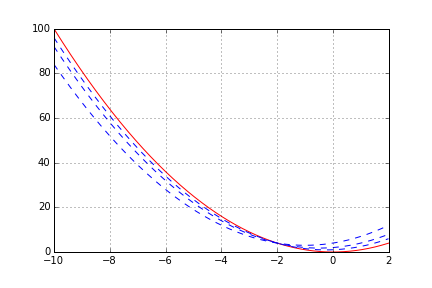
\includegraphics[scale=0.7]{images/convex_opt_04.png}
\end{figure}

The dual function is

\[
g(\lambda) = \inf_x L(x, \lambda) = \inf_x \big\{ x^2 + \lambda (x+2) \big\} = -\frac{\lambda^2}{4} + 2\lambda
\]

which is shown below.

\begin{figure}[H]
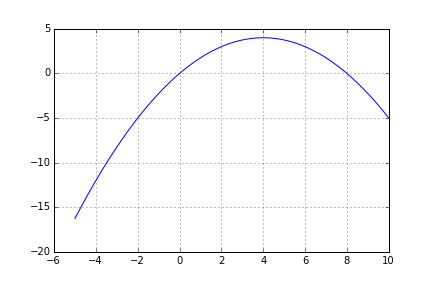
\includegraphics[scale=0.7]{images/convex_opt_04a.png}
\end{figure}

Maximizing (for positive $\lambda$) we have $\lambda^\star=4$ and $d^\star = g(\lambda^\star) = 4$ - again this is in line with the solution of the original problem above.

\subsubsection{Interpretation}

The Lagrangian can be interpreted as follows: Actually we want to
minimize the function

\[
f(x) + \sum_i \mathcal{I}_-(f_i(x)) + \sum_i \mathcal{I}_0(h_i(x))
\]

where the indicator functions are defined as

\[
\mathcal{I}_-(u)=
\begin{cases}
0, \quad u \leq 0 \\
\infty , \quad u > 0
\end{cases}
\]

and

\[
\mathcal{I}_0(u)=
\begin{cases}
0, \quad u = 0 \\
\infty , \quad u \neq 0
\end{cases}
\]

These indicator functions describes the ``displeasure'' with the
equality / inequality constraints: if they are violated, our displeasure is infinite; otherwise we are not unsatisfied. The two $\mathcal{I}_-, \mathcal{I}_0$ are brick-wall functions; even a small violation yields radical displeasure. If we instead use linear displeasure functions, we arrive at the Lagrangian. The more inequality and equality constraints are violated, the larger the two sum terms $ \sum\_i \lambda\_i f\_i(x) + \sum\_i \nu\_i h\_i(x) $ become.

The solution $\tilde x$ of the optimization problem is either (i) inside the feasible region or (ii) located at the border of the feasible region.

In the first case, the derivative of the objective function alone
vanishes because $\tilde x$ is an optimum; i.e. $\nabla f(\tilde x) = 0$. However, the derivative of the Lagrangian $L(x,\lambda,\nu) = f(x) + \sum_i \lambda_i f_i(x) + \sum_i \nu_i h_i(x)$ will \textbf{not} vanish, because the inequality constraints are less than zero in the feasible region: $f_i(\tilde x)\leq 0$. For the
KKT condition $\eqref{kkt5}$ to hold, the Lagrangian multipliers $\lambda$ must be zero.

In the second case, the derivative of the objective function alone will \textbf{not} vanish; for example see the second example above. In this case, the Lagrangian multipliers $\lambda$ will be unequal zero, so that the derivative of the Lagrangian is zero.

If considering problems with order higher than one, these considerations apply for each dimension - see the next example.

\subsubsection{Example 2}

This time consider a two-dimensional function


\begin{align*}
\min f(x,y) &= x^2 + y^2 \\
\text{s.t.} \, 1-x & \leq 0 \\
-1-y & \leq 0
\end{align*}


The Lagrangian is $L = x^2 + y^2 + \lambda_1(1-x) + \lambda_2(-1-y)$. Taking derivatives, we obtain


\begin{align*}
\frac{\partial L}{\partial x} & = 2x - \lambda_1 \\
\frac{\partial L}{\partial y} & = 2y - \lambda_2
\end{align*}


Considering $\lambda_1(1-x)=0$, we have $\lambda_1=0, x=0$ which is not a solution as it is not a feasible point. The other solution, $\lambda_1=2, x=1$ is a valid solution. From $\lambda_2(-1-y)=0$ we find that $\lambda_2=0, y=0$ is a feasible point, whereas $\lambda_2=-2, y=-1$ is not.

This example is a case where the solution for the x-axis is constrained by an inequality constraint, therefore the corresponding
$\lambda_1 \neq 0$. The solution alone the y-axis is not constrained, therefore the corresponding $\lambda_2 = 0$.

The contour plot is given below with the black point ($x=1, y=0$) being the solution.

\begin{figure}[H]
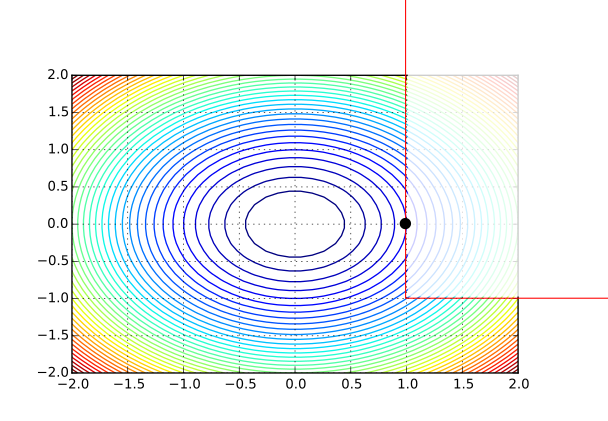
\includegraphics{images/convex_opt_05.png}
\end{figure}

%\DiaryEntry{Convex Optimization - 3}{2015-12-07}{Optimization}

TODO

%\includegraphics{/images/convex_opt_alg_01.jpg}
%\includegraphics{/images/convex_opt_alg_02.jpg}
%\includegraphics{/images/convex_opt_alg_03.jpg}
%\includegraphics{/images/convex_opt_alg_04.jpg}
%\includegraphics{/images/convex_opt_alg_05.jpg}
%\includegraphics{/images/convex_opt_alg_06.jpg}
%\includegraphics{/images/convex_opt_alg_07.jpg}
%\includegraphics{/images/convex_opt_alg_08.jpg}

%\DiaryEntry{Elevator Problem}{2015-12-15}{Maths}

\subsection{Elevator Problem, allowing multiple selection of the same
Floor}

Consider an elevator stopping at $n$ different floors. There are $k$ people using the elevator and every person selects a floor by pressing a button. The selection of $k$ floors (by $k$ people) is denoted as $(f_1,f_2,\cdots,f_k) $ where $f_i$ is the floor selected by the $i$-th person. Different people may select the same floor; i.e.~sequences like $(1,1,3)$ are allowed.

What is the probability that $k$ consecutive floors are selected (e.g. (1,2,3) or (4,5,6)?

First, note that we count (1,2,3) and (3,1,2) as two different sequences.

With this assumption, there are $n^k$ possibilities to press $k$ buttons out of $n$.

In order to count the number of ``good'' cases (i.e.~consecutive floors), assume that the first $k$ floors are pressed; i.e.~we have $ (1,2,\ldots,k) $. The order of the buttons does not matter, so we can arrange the sequence in $k!$ different ways (k possibilities for the first element, k-1 for the second and so on). E.g. for $k=3$ we have (1,2,3), (2,1,3), (3,2,1), (2,3,1), (3,1,2), and (1,3,2).

The first set has the form $1,2,\ldots,k$, the second has the form $(2,3,\ldots,k+1)$, and the last set $(n-k+1,n-k+2,\ldots,n)$. In total we have $n-k+1$ sets. E.g. for $k=3$ and $n=5$, we have $(1,2,3)$, $(2,3,4)$, $(3,4,5)$.

So the total number of ``good'' cases is $k!(n-k+1)$ and therefore the probability that $k$ consecutive buttons are pressed is

\[
P = \frac{k!(n-k+1)}{n^k}
\]

The Figure below show the probability for $n=13$ as a function of $k$. For $k=1$ it is $1$, as any sequence of length 1 is consecutive. For larger $k$, the probability decreases quickly.

\begin{figure}[H]
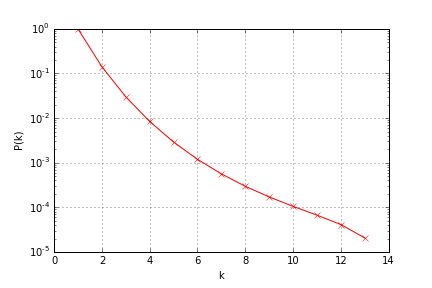
\includegraphics[scale=0.7]{images/elevator.png}
\end{figure}

The Figure below show the probability for $k=10$ as a function of $n$. The probability decreases quickly.

\begin{figure}
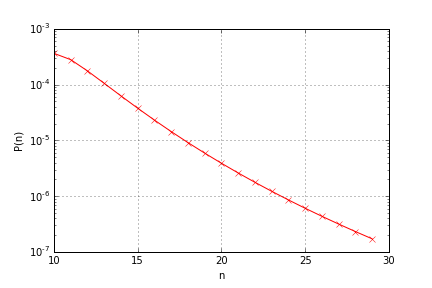
\includegraphics[scale=0.7]{images/elevator_2.png}
\end{figure}

\subsubsection{Additional}

The probability expression above leads to the question how a function

\[
f(k) = \frac{k!}{n^k}
\]

behaves. A plot of the function for $n=10$ (red) and for $n=15$ (blue) is shown below.

\begin{figure}
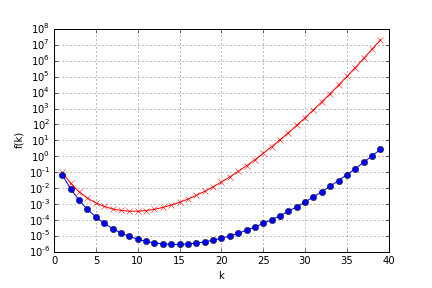
\includegraphics[scale=0.7]{images/factorial_vs_exp.png}
\end{figure}

We first inspect the interesting point $k=n$: We have $f(n) = \frac{n!}{n^n}$. The point to the left, $k=n-1$ yields the following interesting value:

\[
f(n-1) = \frac{(n-1)!}{n^{n-1}} = \frac{(n-1)! n }{n^{n-1} n } = \frac{n!}{n^{n}} = f(n)
\]

Nice :-)

Going further to the left, we have for positive $l$

\[
\frac{f(n-l)}{f(n-l+1)} = \frac{ \frac{(n-l)!}{n^{n-l}} }{ \frac{(n-l+1)!}{n^{n-l+1}} } = \frac{  (n-l)! n^{n-l+1}  }{ (n-l+1)! n^{n-l} } = \frac{n^{n-l+1-(n-l)}}{n-l+1} = \frac{n}{n-l+1} > 1, \, l > 1
\]

which proves that $f(k)$ is larger than $f(n)$ for $k\textless{}n-1$.

A similar argument can be made for points right of $n$. Here we have:

\[
\frac{f(n+l)}{f(n+l+1)} = \frac{ \frac{(n+l)!}{n^{n+l}} }{ \frac{(n+l+1)!}{n^{n+l+1}} } = \frac{  (n+l)! n^{n+l+1}  }{ (n+l+1)! n^{n+l} } = \frac{n^{n+l+1-(n+l)}}{n+l+1} = \frac{n}{n+l+1} < 1, \, l \geq 1
\]

which proves that $f(k)$ is larger than $f(n)$ for $k>n$.

This is the (more) interesting part - for large enough $k$, $k!$ grows larger than $n^k$.

\subsection{Elevator Problem, single selection of the same Floor}

In case we do not allow the selection of the same floor (button) by
different people, the only thing that changes is the total number of
cases: Before we had \(n^k\) (as all \(k\) persons were allowed to press one of the \(n\) floors), now after the first person has chosen one of the \(n\) floors, the second one has only \(n-1\) possibilities left and so on. So in total there are \(n \times (n-1) \times \cdots \times (n-k+1)\) possibilities. We can rewrite this as \(n!(n-k)!\) and so the probability becomes

\[
P^\star = \frac{k!(n-k+1)}{n!/(n-k)!}
\]

Comparing the two probabilities, we see that \(n^k\) is always larger
than \(n!/(n-k)!\) (in the first case we multiply n k-times; in the
second one, the first factor is n, then n-1 and so on). The nominator is the same, therefore, the probability \(p^\star\) is larger than \(P\). This makes sense, as allowing only single selection of the same floor results in a smaller number of total cases.

As an interesting sidenote (regarding simulation), it is only possible to have less persons than floors, i.e. \(k \leq n\) - otherwise not all persons cannot press different floors.

%\DiaryEntry{Combinatorics, 1}{2015-12-20}{Combinatorics}

\subsection{Consecutive Elements in Permutations}

Given a set \(\mathcal{S}_n = \{1,2,3,\ldots,n\}\) and consider
permutations of this set (there are \(n!\) of them). How many
permutations are there, with \(1\) directly followed by a \(2\), up to
\(k\)?

For example, have \(n=4\) and \(k=2\), then a ``valid'' permutation is
\((3,1,2,4)\).

Consider a permutation where the sequence \((1,2,\ldots,k)\) is at the
beginning:

\[
(1,2,\ldots,k,x,\ldots,x)
\]

where \(x\) denotes any number from \(k+1\) to \(n\). These are \(n-k\)
numbers and there are \((n-k)!\) possibilities to place them.

Next we shift the ``\((1,2,\ldots,k)\) group'' one place to the right

\[
(x, 1,2,\ldots,k,x,\ldots,x)
\]

Again, there are \((n-k)!\) possibilities to place the \(x\) values.

We note that there are \(n-k+1\) ways to place the ``\((1,2,\ldots,k)\)
group'' (from the very left to the very right); thus in total there are
\((n-k+1)(n-k)!\) permutations.

\subsubsection{Extreme Cases}

For \(k=n-1\) we obtain for the number of permutations
\([n-(n-1)+1][n-(n-1)]! = 2+1! = 2\). There are only two possibilities
of the form ``\((1,2,\ldots,k,n)\) and''\((n,1,2,\ldots,k)\).

For \(k=1\) we have \((n-1+1)(n-1)! = n(n-1)! = n!\): We are free to
place all elements in any order - therefore we get the numbe of
permutations of the original set \(\mathcal{S}_n\).

\subsubsection{Example for \(n=4\)}

Below the ``good'' cases are shown. The values 3 and 4 can be placed
onto the x's; for each row, there are \(2!=2\) ways to place them
(\((3,4)\) and \((4,3)\)). Therefore in total there are
\(3 \times 2 = 6\) possible placements.


\begin{align*}
&(1,2,x,x)\\
&(x,1,2,x)\\
&(x,x,1,2)
\end{align*}


\subsection{Number of Words}

The number of words with length \(k\) in an alphabet with \(n\) elements
is \(n^k\). This is easy. Now add the constraint, that two consecutive
letters must be different.

The first letter can be chosen independently, so we have \(n\)
possibilities. The second letter must be different from the first,
therefore there are only \(n-1\) possibilities left. This argument holds
for all letters except the first; therefore, there are \(n(n-1)^{k-1}\)
possibilities.

\subsection{Set-Partitioning into 2 Subsets}

The set \(\mathcal{S}\) has \(n\) elements. In how many ways can the set
be partitioned into two subsets \(\mathcal{A}\) and \(\mathcal{B}\)
which are not necessarily disjoint and whose union is \(\mathcal{S}\):
\(\mathcal{A} \cup \mathcal{B} = \mathcal{S}\).

For every element \(x \in \mathcal{S}\), there are three cases:

\begin{itemize}
\item
  \(x \in \mathcal{A}, x \notin \mathcal{B}\)
\item
  \(x \notin \mathcal{A}, x \in \mathcal{B}\)
\item
  \(x \in \mathcal{A}, x \in \mathcal{B}\)
\end{itemize}

Therefore, there are \(3^n\) ways to choose \(\mathcal{A}\) and
\(\mathcal{B}\).

We can arrive at this result via induction as well. Start with \(n=1\);
i.e. \(\mathcal{S} = \\{1\\}\). Then we can place (i) 1 into
\(\mathcal{A}\) and leave \(\mathcal{B}\) empty, (ii) place 1 into
\(\mathcal{B}\) and leave \(\mathcal{A}\) empty or (iii) put 1 into both
\(\mathcal{A}, \mathcal{B}\).

So, for \(n=1\), we have \(3\) possibilities. If we add a second element to \(\mathcal{S}\), we use the same argument for placing the second element \textbf{independently} form the first one. Therefore, there are \(3^n\) ways to select the subsets.

Note that the Stirling Numbers of the second kind \({n \brace k}\) count the number of \(n\) elements into \(k\) \textbf{non-empty} partitions. For \(k=2\), we have the special relation \({n \brace 2} = 2^{n-1}-1\).

We can prove this as follows: A binary string \((b_1, \ldots,b_n)\)
represents a partition. If \(b_i = 0\), then \(i \in \mathcal{A}\), if \(b_i = 1\), then \(i \in \mathcal{B}\). The all-zero and the all-one string are not allowed as the would leave one of the two sets empty. Furthermore, we double count; i.e.~we treat
\(\mathcal{A} = \{1,2\}, \mathcal{B} = \{3\}\) and \(\mathcal{A} = \{3\}, \mathcal{B} = \{1,2\}\) as separate partitions (which they are not). Therefore, we have \({n \brace 2} = \frac{2^{n}-2}{2} = 2^{n-1}-1\).

%\DiaryEntry{Permutations, 1}{2015-12-20}{Combinatorics}

There is a rather good and comprehensive Wikipedia
\href{https://en.wikipedia.org/wiki/Permutation}{article}.

Short summary:

\begin{itemize}
\item
  There is a set of items \(\mathcal{S}\).
\item
  We consider ``arrangements'' of the element's set. E.g.
  \(\mathcal{S} = \\{1,2,3\\}\). Arrangement in this context means, that
  the elements are reshuffled.
\item
  No duplicates are allowed i.e.~no \((1,1,2)\) and order is important;
  i.e. \((1,2,3) \neq (1,3,2)\).
\end{itemize}

If the set has size \(k\), i.e. \(\|\mathcal{S}\| = k\), there are
\(k!\) permutations possible: The first position can be filled with
\(k\) different values, the second position can be filled with \(k-1\)
and so on, till only one element is left for the \(k\)-th position.

\subsubsection{Bijection Interpretation}

Seen another way, a permutation is a bijection from \(\mathcal{S}\) onto
\(\mathcal{S}\). A bijection is a one-to-one function. This view allows
to interpret a permutation as a function (mapping from \(\mathcal{S}\)
to \(\mathcal{S}\)) and can be composed.

The two-line notation lists the elements of \(\mathcal{S}\) in the first
row and the image (the ``permutation's output'') on the second row.

For example, we have

\[
\sigma=\begin{pmatrix}
1 & 2 & 3 & 4 & 5 \\
2 & 5 & 4 & 3 & 1\end{pmatrix}
\]

which means that 1 is mapped onto 2 (written as \(\sigma(1) = 2\)), 2 is
mapped onto 5 (\(\sigma(2) = 5\)) and so on.

The permutation does not change when the columns are rearranged;
e.g.~above permuation can also be rewritten as

\[
\sigma=
\begin{pmatrix}
2 & 5 & 4 & 3 & 1 \\
5 & 1 & 3 & 4 & 2
\end{pmatrix}
\]

\subsubsection{Permutation Cycles}

If we repeatedly apply the permutation to an element \(x\) we obtain a
sequence \(x, \sigma(x), \sigma(\sigma(x)), \cdots\). After some length,
the sequence will return to the initial element \(x\) and the
corresponding sequence is called an orbit / cycle of the permutation.
Choosing any other value from \(\mathcal{S}\) which is not element of
the orbit, one obtains another orbit and so on until all element of
\(\mathcal{S}\) are covered. A permutation can also be represented by
listing it cycles.

The cycles of the permutation above are \((1,2,5), (3,4)\). Note that
the representation is not unique; e.g. \((2,5,1), (4,3)\) represents the
same permutation.

A cycle of length k is called a \(k\)-cycle. An element in a \(1\)-cycle
is a fixed point of the permutation \(\sigma\): The element does not
change position under the permutation.

A permutation without a \(1\)-cycle is called a derangement; in this
case, all element are placed into a new position and no element stays on
its position.

\subsubsection{Permutation Composition}

Composition of two permutations \(\sigma_1, \sigma_2\) means that first
the permutation \(\sigma_1\) is applied to a sequence \(x\) and then the
second permutation \(\sigma_2\) is applied to the result; i.e.
\(\sigma_2(\sigma_1(x))\).

The composition can be obtained by rearranging the columns of the second
(leftmost) permutation so that its first row is identical with the
second row of the first (rightmost) permutation. The product can then be
written as the first row of the first permutation over the second row of
the modified second permutation. For the example permutation above we
obtain

\[
\sigma(\sigma) = 
\begin{pmatrix}
2 & 5 & 4 & 3 & 1 \\
5 & 1 & 3 & 4 & 2
\end{pmatrix}
\begin{pmatrix}
1 & 2 & 3 & 4 & 5 \\
2 & 5 & 4 & 3 & 1
\end{pmatrix}
=
\begin{pmatrix}
1 & 2 & 3 & 4 & 5 \\
5 & 1 & 3 & 4 & 2
\end{pmatrix}
\]

From the result the effect of the \(2\)-cycle \((3,4)\) can be seen
clearly.

Multyplying the permutation in a third time, we obtain

\begin{align*}
\sigma(\sigma(\sigma)) &= 
\begin{pmatrix}
1 & 2 & 3 & 4 & 5 \\
2 & 5 & 4 & 3 & 1
\end{pmatrix}
\begin{pmatrix}
1 & 2 & 3 & 4 & 5 \\
5 & 1 & 3 & 4 & 2
\end{pmatrix}
=
\begin{pmatrix}
5 & 1 & 3 & 4 & 2 \\
1 & 2 & 4 & 3 & 5
\end{pmatrix}
\begin{pmatrix}
1 & 2 & 3 & 4 & 5 \\
5 & 1 & 3 & 4 & 2
\end{pmatrix}
 \\ & =
\begin{pmatrix}
1 & 2 & 3 & 4 & 5 \\
1 & 2 & 4 & 3 & 5
\end{pmatrix}
\end{align*}

Now the effect of the \(3\)-cycle becomes visible; the \(2\)-cycle
exchanges elements \(3\) and \(4\).

In general the composition of two permutations is not commutative, but
it is associative.

The identity permutation, which maps every element of the set to itself,
is the neutral element for this product and has the following form:

\[
\begin{pmatrix}
1 & 2 & 3 & \ldots & n \\
1 & 2 & 4 & \ldots & n
\end{pmatrix}
\]

Since a permutation is a bijection, it has an inverse \(\sigma^{-1}\)
which can be obtain by exchanging the first and second line (followed by an optional rearrangement of columns):

\[
\sigma^{-1} = 
\begin{pmatrix}
1 & 2 & 3 & 4 & 5 \\
2 & 5 & 4 & 3 & 1
\end{pmatrix}^{-1} = 
\begin{pmatrix}
2 & 5 & 4 & 3 & 1 \\
1 & 2 & 3 & 4 & 5
\end{pmatrix}
=
\begin{pmatrix}
1 & 2 & 3 & 4 & 5\\
5 & 1 & 4 & 3 & 2
\end{pmatrix}
\]

In order to check the result, we compose \(\sigma\) with \(\sigma^{-1}\)
and obtain

\[
\begin{pmatrix}
1 & 2 & 3 & 4 & 5 \\
2 & 5 & 4 & 3 & 1
\end{pmatrix}
\begin{pmatrix}
1 & 2 & 3 & 4 & 5\\
5 & 1 & 4 & 3 & 2
\end{pmatrix}
=
\begin{pmatrix}
5 & 1 & 4 & 3 & 2 \\
1 & 2 & 3 & 4 & 5
\end{pmatrix}
\begin{pmatrix}
1 & 2 & 3 & 4 & 5\\
5 & 1 & 4 & 3 & 2
\end{pmatrix}
=
\begin{pmatrix}
1 & 2 & 3 & 4 & 5\\
1 & 2 & 3 & 4 & 5
\end{pmatrix}
\]

which is the identity permutation again.

\subsubsection{Matrix Representation}

We can also represent a permutation in matrix notation; the
\(n \times n\) matrix associated with the permutation \(\sigma\) has one
\(1\) in every row and every column and is zero otherwise. The entry
\(M_{i,j}\) of the matrix is one if \(\sigma(j) = i\). From this it can
be clearly seen that permutation composition is not commutative.
Furthermore, the identity permutation becomes the \(n \times n\)
identity matrix.

For our example, we have the following matrix

\[
M = 
\begin{pmatrix}
0 & 1 & 0 & 0 & 0\\
0 & 0 & 0 & 0 & 1\\
0 & 0 & 0 & 1 & 0\\
0 & 0 & 1 & 0 & 0\\
1 & 0 & 0 & 0 & 0
\end{pmatrix}
\]

In the matrix \(M_{3,4} = 1\) because \(\sigma(4 = 3\).

%\DiaryEntry{Permutations, 2}{2015-12-26}{Combinatorics}

As stated before, a permutation is a bijection (one-to-one mapping) from \(\mathcal{S}\) onto \(\mathcal{S}\).

A permutation can have fixed points; i.e.~elements \(x^\star\) which
stay constant under the mapping: \(\sigma(x^\star) = x^\star\).

The opposite to fixed points are derangements, which are permutations of the elements, such that no element appears in its original position.

If we take \(\mathcal{S} = \{1,2,3,4\}\), then there are \(4!\)
permutations. Out of these, the derangements are as follows


\begin{align*}
    & (2,1,4,3), (2,3,4,1), (2,4,1,3) \\
    & (3,1,4,2), (3,4,1,2), (3,4,2,1) \\
    & (4,1,2,3), (4,3,1,2), (4,3,2,1) \\ 
\end{align*}


We will denote with \(!n\) the number of derangements of \(n\) elements;
from above example it follows that \(!3 = 9\).

\subsubsection{Recurrence Relation}

Let's consider the permutation of the first position \(\sigma(1) = i\)
with \(i \neq 1\). There are \(n-1\) way to select such an \(i\). Next
we need to select a value for \(\sigma(i)\). There are two options:

\begin{itemize}
\item
  We choose any \(i \neq 1\) (and \(\sigma(i) \neq i\)). In this case we
  have a derangement with \(n-1\) elements.
\item
  We choose \(\sigma(i)=1\), in this case a derangement with \(n-2\)
  elements remains.
\end{itemize}

Combining these two options (and considering that we can select the
original \(i\) in \(n-1\) way), we obtain for the number of derangements

\begin{equation}
\label{recur}
!n = (n-1) \left[ !(n-1) +  !(n-2)\right]
\end{equation}

The initial conditions are \(!0=1\) and \(!1=0\). The next values are
then (starting with \(n = 2\))

\[
1, 2, 9, 44, 265, 1854, 14833, 133496, 1334961, 14684570, 176214841, 2290792932, \cdots
\]

which is \href{https://oeis.org/A000166}{OEIS sequence}. We have
\(!2 = 1\); i.e.~there is only one derangement (which is \((2,1)\)),
\(!3 = 2\), the two derangements are \((2,3,1)\) and \((3,1,2)\).

\subsubsection{Relation with Factorial}

As the factorial counts the number of \emph{all} permutations and not
all permutations are derangements, we have \(!n < n!\).

First observe that we have the same recurrence relation as
\(\eqref{recur}\) for the factorials:

\begin{equation}
\label{recur2}
n!= (n-1) \left[ (n-1)! +  (n-2)!\right]
\end{equation}

because

\[
n(n-1)! - (n-1)! + (n-2)! (n-1) = n! - (n-1)! + (n-1)! = n!
\]

Dividing \(\eqref{recur}\) by \(\eqref{recur2}\), we have

\[
\frac{!n}{n!} = \frac{ (n-1) \left[ !(n-1) +  !(n-2)\right] }{ (n-1) \left[ (n-1)! +  (n-2)!\right] }
\]

\subsection{Add-on}

Some more stuff can be found
\href{http://math.ucr.edu/home/baez/qg-winter2004/derangement.pdf}{here}.

%\DiaryEntry{Relations between Random Variables}{2016-01-03}{Stochastic}

\subsection{RVs with different Distribution}

Consider two RVs \(X_1, X_2\) which are independently distributed with
pdfs \(f_1(u)\), \(f_2(u)\) and cdfs
\(F_1(u) = \int_{-\infty}^u f_1(v)dv\) and
\(F_2(u) = \int_{-\infty}^u f_2(v)dv\).

We want to calculate the probability that \(X_1 < X_2\):

\[
P(X_1 < X_2) = \int_\alpha P(X_1<\alpha, X_2=\alpha) d\alpha = \int_\alpha F_1(\alpha) f_2(\alpha) d\alpha
\]

\subsubsection{Example: Two Uniform Distributions}

Consider \(X_1\) distributed uniformly on \([0,2]\) and \(X_2\)
distributed uniformly on \([1,3]\). The Figure below shows the cdf
\(F_1(u)\) in red and the pdf \(f_2(u)\) in green:

\begin{figure}[H]
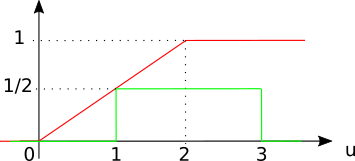
\includegraphics{images/rv_relation_1.png}
\end{figure}

The desired probability then becomes

\[
P(X_1 < X_2) = \int_\alpha F_1(\alpha) f_2(\alpha) d\alpha = \int_{\alpha=1}^{2} \frac{\alpha}{2} \frac{1}{2} d\alpha + \int_{\alpha=2}^{3} 1 \frac{1}{2} d\alpha = \frac{7}{8}
\]

\subsection{RVs with same Distribution}

In the special case that both RVs are distributed the same; i.e.~with
pdf \(f_x(u)\) and cdf \(F_x(u) = \int_{-\infty}^u f_x(v)dv\), the
probability that \(X_1 < X_2\) becomes:

\[
P(X_1 < X_2) = \int_\alpha P(X_1<\alpha, X_2=\alpha) d\alpha = \int_\alpha P(X_1<\alpha) P(X_2=\alpha) d\alpha = \int_\alpha F_X(\alpha) f_x(\alpha) d\alpha
\]

\subsubsection{Example: Uniform Distribution}

If \(X_1, X_2\) are distributed uniformly between 0 and 1, the cdf in
the interval \([0,1]\) becomes \(F_x(u) = u\) and we have

\[
P(X_1 < X_2) = \int_{\alpha=0}^1 \alpha 1 d\alpha = \frac{1}{2}
\]

\subsection{General Result}

This result holds in general; i.e.~for two RVs distributed with the same
pdf, we have \(P(X_1 < X_2) = 1/2\). This can be shown as follows:

\[
P(X_1 < X_2) = \int_{\alpha=-\infty}^\infty F(\alpha) f(\alpha) d\alpha = \int_{\alpha=-\infty}^\infty \int_{u=-\infty}^\alpha f(u) du f(\alpha) d\alpha
\]

Reordering the integrals, we obtain

\[
P(X_1 < X_2) = \int_{\alpha=-\infty}^\infty \int_{u=-\infty}^\alpha f(u) f(\alpha) du d\alpha
\]

Note that the integral over the complete \(\alpha - u\) area yields
\(1\) because we integrate over a (joint) probability function. The
integration region in the double integral above is half the area (see
Figure below), the integrand is rotational symmetric and therefore the
integral yields a value of 1/2.

\begin{figure}[H]

\includegraphics{images/rv_relation_2.png}
\end{figure}

\subsubsection{Conjecture}

$P(X_1 <  X_2) = 1/2$ holds for any two RVs with zero mean and symmetry around the origin.


%%% Local Variables:
%%% mode: latex
%%% TeX-master: "journal"
%%% End:

%\DiaryEntry{Permutations, 3 (Number of Fixed Points)}{2016-01-04}{Combinatorics}

Consider a set of $n$ elements: In total there are $n!$ permutations - How many permutations are there with $k$ fixed points? This number is callled \href{https://en.wikipedia.org/wiki/Rencontres_numbers}{Recontres Number} and will be denoted as $D_{n,k}$.

For example, chose $n=5$ and consider the permutation

\[
\sigma=\begin{pmatrix}
1 & 2 & 3 & 4 & 5 \\
2 & 5 & 3 & 1 & 4
\end{pmatrix}
\]

We have one fixed point: $\sigma(3) = 3$.

In order for a permutation to have \textbf{one} fixed point, any of the $n$ elements can become the fixed point. The other $n-1$ must not have a fixed point, therefore they must form a derangement. There are $!(n-1)$ such derangements. Therefore, the number of permutations with exactly one fixed point is

\bee
D_{n,1} = n !(n-1)
\eee

In a similar way we can argue for the number of permutations having two fixed points: There are $n \choose 2$ ways to select the two fixed points and the other $n-2$ elements must form a derangement.
Therefore, we have

\bee
D_{n,2} = {n \choose 2} !(n-2)
\eee

Generalizing, we obtain

\bee
D_{n,k} = {n \choose k} !(n-k)
\eee

for the number of permutations of $n$ elements having $k$ fixed points.

\subsubsection{Some Values}

can be found \href{https://en.wikipedia.org/wiki/Rencontres_numbers}{here} and are shown below.

\begin{figure}
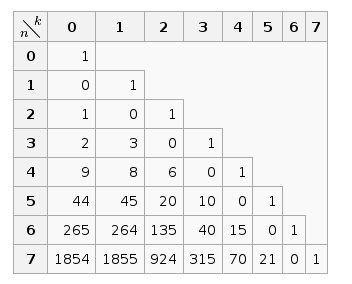
\includegraphics{images/recontres_numbers.png}
\end{figure}

The following properties can be observed:

\begin{itemize}
\item  It can be seen that $D_{n,n-1} = 0$; there are no permutations of $n$ elements having $n-1$ fixed points; the last element must also be a fixed point.
\item  There is one $n$-permutation with $n$ fixed points: $D_{n,n} = 1$ which is the identity permutation.
\item  The number of permutations without a fixed point (i.e. $k=0$) equals the number of derangements; i.e. $D_{n,0} = !n$.
\item  The row-sum equals the number of permutations; i.e. $\sum_{k} D_{n,k} = n!$. We can split the permutations into groups having the same number of fixed points. Summing over the group-sizes yields the total number of permutations.
\end{itemize}

\subsubsection{Probability of $k$ fixed points}

Now let's calculate the probability $P_{n,k}$ that a randomly chosen permutation has $k$ fixed points. We have

\bee
P_{n,k} = {n \choose k} \frac{!(n-k)}{n!}
\eee

Inserting the definition of ${n \choose k} = \frac{n!}{(n-k)! k!}$ and obtain

\bee
P_{n,k} = \frac{n!}{(n-k)! k!} \frac{!(n-k)}{n!} = \frac{!(n-k)}{(n-k)! k!} = \frac{1}{k!} \frac{!(n-k)}{(n-k)!}
\eee

Let's consider this in the case of large $n$; from the previous entry \ref{2015-12-26:entry} we know that $\lim_{n \rightarrow \infty} \frac{!n}{n!} = e^{-1}$ and therefore

\bee
\lim_{n \rightarrow \infty} P_{n,k} = \frac{1}{e k!}
\eee

As a cross-check, the probabilities must sum up to one; $\sum_{k=0}^\infty \frac{1}{e k!} = \frac{e}{e} = 1$ \qed.

We can also calculate the expected number of fixed points; we have

\bee
\sum_{k=0}^\infty k \frac{1}{e k!} = \frac{1}{e} \sum_{k=0}^\infty k \frac{1}{k!} = \frac{1}{e} \sum_{k=0}^\infty \frac{1}{(k-1)!} = \frac{1}{e} e = 1
\eee

So in the limit of large $n$, we have an expected number of one fixed point in a randomly chosen permutation.


%%% Local Variables:
%%% mode: latex
%%% TeX-master: "journal"
%%% End:

%\DiaryEntry{Chi-Square Distribution}{2016-01-18}{Stochastic}

If \(Z_1, \ldots, Z_k\) are iid standard normal RVs, then the sum of
their squares,

\[
Q_k = \sum_{i=1}^k Z_i^2
\]

is distributed according to the chi-squared distribution with \(k\)
degrees of freedom, denoted as \(Q \sim \chi^2 (k)\).

The pdf of a chi-squared distribution with \(k\) degrees of freedom has the following form

\[
f(x; k) = \frac{ x^{k/2-1} e^{-x/2} }{ 2^{k/2} \Gamma(\frac{k}{2}) }; \, x \geq 0
\]

A plot of the distribution for different values of \(k\) can be seen
below:

\begin{figure}[H]
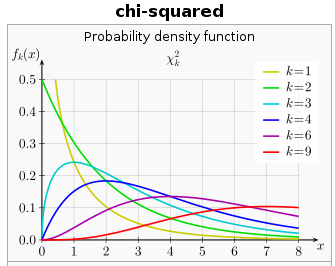
\includegraphics{images/chi-square_01.png}
\end{figure}

For increasing \(k\), the peak of the distribution moves to the right as more and more terms are involved in the summation. This is also consistent with the mean of the chi-squared distribution being equal to \(k\).

\subsubsection{Limit values for \(x=0\)}

For \(k=1\), we have:

\begin{equation}
\label{keqone}
f(x;1) = \frac{e^{-x/2}}{\sqrt{2\pi}\sqrt{x}}
\end{equation}

and this becomes infinity for \(x \rightarrow 0\).

For \(k=2\), we obtain

\[
f(x;2) = \frac{1}{2} e^{-x/2}
\]

and this becomes \(1/2\) for \(x \rightarrow 0\).

Finally, for \(k \geq 3\), the x moves into the numerator, thereby
causing the pdf to become zero for \(x \rightarrow 0\).

\subsubsection{Open Question}

The pdf at \(x=0\) equals the probability that \(Q=0\); i.e.

\[
P\left\{\sum_{i=1}^k Z_i^2=0\right\}
\]

It would be interesting to understand, why this probability is non-zero for 1 and 2 normal RVs and only becomes zero for 3 or more RVs.

Actually, the difference has a smaller effect on the cdf. Here, the
value \(f(0;k)\) only affects the slope of the cdf \(F_Q(x)\) at
\(x=0\). Therefore, the cdf has a zero slope at \(x=0\) for
\(k \geq 3\).

\subsubsection{Special Case \(k=1\)}

In this case, we have \(Q_1 = Z_1^2\) which is actually a RV transformation. We can directly use results from the next entry and arrive at

\[
f(x;1) = \frac{1}{\sqrt{x}} f_Z(\sqrt{x}) = \frac{1}{\sqrt{2 \pi x}} e^{- (\sqrt{x})^2 / 2 } = \frac{1}{\sqrt{2 \pi x}} e^{- x / 2 }
\]

which is exactly the result from \eqref{keqone}.

%\DiaryEntry{Transformation of Random Variables}{2016-01-19}{Stochastic}
\todo{Figure}

%\begin{figure}
%\centering
%\includegraphics{/images/rv_transform_0001.png}
%\caption{Page1}
%\end{figure}

The proof runs somewhere along the line that we calculate

\[
P(Y < a) = \int_{-\infty}^a f_Y(u) du
\]

and differentiate with respect to \(a\) in order to obtain \(f_Y\).

We make a substitution to evaluate the integral in terms of \(f_X\). In
order to do that, the bounds change, the integrand is changed to
\(f_X(g^{-1}(v))\), and finally the derivative of \(g^{-1}\) sneaks in.

It is interesting to see, that whenever \(g(x)\) has a zero slope, the
pdf \(f_Y\) attains a value of \(\infty\).

\todo{figure}

%\begin{figure}
%\centering
%\includegraphics{/images/rv_transform_0002.png}
%\caption{Page1}
%\end{figure}

\hypertarget{appendix-a}{%
\subsubsection{Appendix A}\label{appendix-a}}

If we consider the example of \(g(x) = x^2\), then both \(x=-1\) and
\(x=1\) contribute to \(y=1\). Therefore, we need to sum the RV
transformation formula over all values \(x\) which contribute to the
same value of \(y\).

\hypertarget{example}{%
\subsubsection{Example}\label{example}}

\todo{figure}

%\begin{figure}
%\centering
%\includegraphics{/images/rv_transform_0003.png}
%\caption{Page1}
%\end{figure}

If we have another transform function we have

\[
f_Y(y) = \sum_{y = g(x)}\left| \frac{d g^{-1}(y)}{dy} \right| f_X(g^{-1}(y))
\]

where the summation indicates to sum over all values of \(x\) which
yield \(y = g(x)\).

If we have a symmetric distribution of \(X\), the expression simplifies
to

\[
f_Y(y) = 2 \left| \frac{d g^{-1}(y)}{dy} \right| f_X(g^{-1}(y))
\]

%\DiaryEntry{Continuity, 1}{2016-01-24}{Topology}

\subsubsection{Classical Definition}

Given any subset \(\mathcal{S}\) of \(\mathcal{R}\), a function
\(f : \mathcal{S} \rightarrow \mathcal{R}\) is continuous at a point
\(a\) in its domain \(\mathcal{S}\) if: For every \(\epsilon > 0\), it
is possible to find a \(\delta > 0\) such that

\[
| f(x) - f(a) | < \epsilon \,\, \text{for} \,\, |x-a| < \delta
\]

The idea is as follows: We allow for a certain variation \(\epsilon\) of
the function values and ask for the interval in which this variation
takes place. For a fixed variation, we are allowed to choose an
arbitrary small \(\delta\); however, it is important, that such a
\(\delta\) exists and can be found at all.

The Figure below shows a function being continuous at \(x=a\) on the
left, and a function being discontinuous at \(x=a\).

On the left, we can \textbf{always} find a \(\delta\) for every value
\(\epsilon\) we choose. On the right, it is not possible to find a
\(\delta\) for values of \(\epsilon\) smaller than the jump at \(x=a\).

\begin{figure}[H]
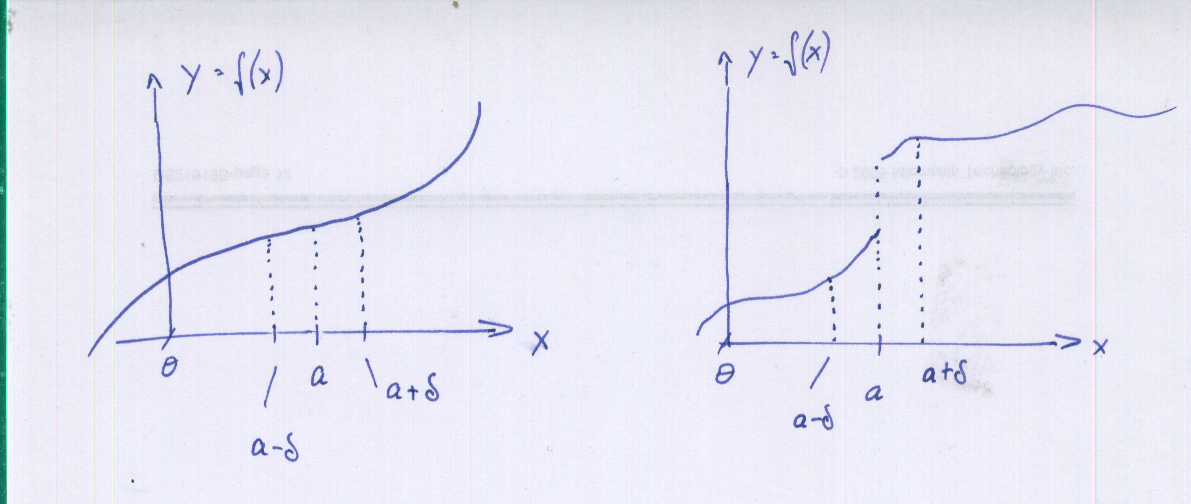
\includegraphics[scale=0.7]{images/continuity_01.png}
\end{figure}

\subsubsection{Example}

Consider the function \(f(x)=x^2\). At \(x=2\), we have the following
two equations:


\begin{align}
(2+\epsilon)^2 & = 2+\delta \\
(2-\epsilon)^2 & = 2-\delta
\end{align}


For \textbf{any value} \(\epsilon\), we can solve both equations for
\(\delta\) (the ``final'' \(\delta\) is the larger of the two).

Now consider the function given by

\[
f(x) = \begin{cases}
0 & \mbox{if } x \leq 0 \\
1 & \mbox{if } x > 0 \end{cases}
\]

If we consider \(x=0\), where \(y=0\), then we can choose a value of
\(\epsilon=1/2\) for which no value \(\delta\) can be found.

%\DiaryEntry{AM-GM Inequality}{2016-02-02}{Maths}

Proof that

\[
(a_1 \cdots a_n)^{1/n} \leq \frac{a_1 + \cdots + a_n}{n}
\]

For \(n=2\) this is easy: We have
\((x-y)^2 = x^2 + y^2 - 2xy \geq 0 \rightarrow \frac{x^2 + y^2}{2} \geq xy\).
If we replace \(x\) with \(\sqrt{x}\) and \(y\) with \(\sqrt{y}\), we
arrive at

\[
\frac{x + y}{2} \geq \sqrt{xy}
\]

For \(n=4\), we apply the inequality for \(n=2\) two times: The first
time to \((a_1 a_2)^{1/2}\) and \((a_3 a_4)^{1/2}\):

\[
(a_1 a_2 a_3 a_4)^{1/4} = \left( (a_1 a_2)^{1/2}(a_3 a_4)^{1/2} \right)^{1/2} \leq \frac{(a_1 a_2)^{1/2} + (a_3 a_4)^{1/2}}{2}
\]

Applying the inequality a second time to we arrive at

\[
(a_1 a_2 a_3 a_4)^{1/4} \leq \frac{1}{2} \frac{a_1 + a_2}{2} + \frac{1}{2} \frac{a_3 + a_4}{2} = \frac{a_1 a_2 a_3 a_4}{4}
\]

By repeatedly applying this inequality, we can extend to cases
\(n = 2^k\):

\begin{equation}
\label{eq:amgm2k}
(a_1 a_2 \cdots a_{2^k})^{1/2^k} \leq \frac{a_1 + \cdots + a_{2^k}}{2^k}
\end{equation}

The question is how to proof the inequality for general \(n\). To this
end we take an \(n < 2^k\) and define a sequence \(\alpha_i\) as
follows:

\[
\alpha_i = \begin{cases}
a_i & \mbox{if } i \leq n \\
A & \mbox{if } i > n \end{cases}
\]

where \(A = \frac{a_1 + \cdots + a_n}{n}\). In other words, we simply
pad the original sequence \(a_i\) with the arithmetic average \(A\) to
give a length-\(2^k\) sequence. The average \(A\) is contained
\(2^k - n\) times in the sequence \(\alpha_i\) and therefore equation
\eqref{eq:amgm2k} yields

\[
(a_1 a_2 \cdots a_n A^{2^k - n})^{1/2^k} \leq \frac{a_1 + \cdots + a_n + (2^k - n) A}{2^k} = \frac{nA + 2^k A - nA}{2^k} = A
\]

We can move the \(A\) term to the right side as follows:

\[
(a_1 a_2 \cdots a_n)^{1/2^k} A^{(2^k - n)\frac{1}{2^k}} = (a_1 a_2 \cdots a_n)^{1/2^k} A^{1 - \frac{n}{2^k}} \leq A \rightarrow (a_1 a_2 \cdots a_n)^{1/2^k} \leq A^{1 - (1 - \frac{n}{2^k})} = A^{\frac{n}{2^k}}
\]

Raising both sides to \(2^k / n\), we finally obtain the AM-GM
inequality

\[
(a_1 a_2 \cdots a_n)^{1/n} \leq A = \frac{a_1 + \cdots + a_n}{n}
\]

%\DiaryEntry{Cauchy Inequality}{2016-02-02}{Maths}

Any norm \(d(x,y)\) must fulfill four properties:

\begin{itemize}
\item
  It must be positive for any \(x,y\): \(d(x,y) \leq 0\).
\item
  It must be only zero if and only if \(x = y\)
\item
  It must be commutative; i.e. \(d(x,y) = d(y,x)\)
\item
  It must fulfill the triangle inequality:
  \(d(x,y) \leq d(x,z) + d(z, y)\)
\end{itemize}

One norm function is the Euclidian norm; for a d-dimensional space it
has the following form:

\[
d(x,y) = \sqrt{(y_1 - x_1)^2 + \cdots + (y_d - x_d)^2}
\]

The first three norm properties are quite straightforward; the triangle
inequality can be shown using the Cauchy inequality as follows.

Without loss of generality, we can set \(x = 0\), \(y = u+v\), and
\(z = v\) in the triangle inequality. Note that the Euclidian norm is
translation invariant; i.e. \(d(x+w, y+w) = d(x,y)\) for all \(w\). This
allows to express the triangle inequality as follows:

\[
d(0, u+v) \leq d(0, v) + d(v, u+v) = d(0, v) + d(0, u)
\]

where the last equality follows from translation invariance. Inserting
the definition of the norm into the last expression, we obtain:

\[
\sqrt{\sum(u_j + v_j)^2} \leq \sqrt{\sum u_j^2} + \sqrt{\sum v_j^2}
\]

Squaring both sides, we obtain

\[
\sum(u_j + v_j)^2 = \sum u_j^2 + 2 \sum u_j v_j + \sum v_j^2 \leq \sum u_j^2 + 2 \sqrt{\sum u_j^2} \sqrt{\sum v_j^2} + \sum v_j^2
\]

and cancelling terms on both sides yields

\[
\sum u_j v_j  \leq \sqrt{\sum u_j^2} \sqrt{\sum v_j^2}
\]

which is exactely the Cauchy inequality.

%\DiaryEntry{Continuity, Topological Definition}{2016-02-03}{Topology}

\subsection{Open and Closed Intervals}

An open interval \((a,b)\) is defined as the set

\[
(a,b) = \{ x \in \mathcal{R}: a < x < b \}
\]

Note that the open interval does not include the endpoints. A closed
interval does include the end points; i.e.~it is defined as the set

\[
[a,b] = \{ x \in \mathcal{R}: a \leq x \leq b \}
\]

A union of open intervals is not necessarily an open interval again;
e.g. \((0,1) \cup (3,4)\) is not an open interval as it is not possible
to write the union in the form \((a,b)\).

\subsection{Open and Closed Sets}

Instead such a union is called an open set - formally it is defined as:
Let \(\mathcal{S}\) denote a subset of \(\mathcal{R}\). Then
\(\mathcal{S}\) is open, if for every point \(x \in \mathcal{S}\), there
is some open interval \((x-\delta_x, x + \delta_x)\) (\(\delta_x > 0\))
contained in \(\mathcal{S}\).

Consider the example of the open set \(\mathcal{S} = (0,1)\). The point
\(0.1\) is in \(\mathcal{S}\); in addition, we can construct an open
interval \((0.05, 0.15)\) around \(0.1\) which is contained in
\(\mathcal{S}\). Because the endpoints are not included in the open set,
we can continue this argument for any point, no matter how close to the
end point it is: The point \(\epsilon\) (with \(\epsilon \ll 1\)) can
always be surrounded by an open interval \((\epsilon/2, 3\epsilon/2)\),
which is still contained in \(\mathcal{S}\).

In case of an open set this argument is not possible: If we consider a
closed set \(\mathcal{S} = [a,b]\), then we cannot find an open interval
around \(a\) (or \(b\)), which is still contained in \(\mathcal{S}\) -
no matter how small the open interval. The open interval
\((a-\epsilon, a+\epsilon)\) will always be half outside
\(\mathcal{S}\).

Another interpretation of the open interval in the definition above is
that it forms a ``breathing space'' for the point \(x\).

We can repeat above arguments for a union of open intervals and see that
for every point of the intervals, we can find such a breathing space.
Therefore the union of open intervals is an open set.

\subsubsection{Special Cases}

The whole real line \(\mathcal{R}\) is an open set: For every
\(x \in \mathcal{R}\), we can find a neighbourhood which will be
contained in \(\mathcal{R}\).

Conversely, the empty set is also (defined to be) open: There is no
\(x\) around which a breathing space must exist, therefore the set is
open.

\subsubsection{Union and Intersection}

\begin{itemize}
\item
  The union of any collection of open sets is open.
\item
  Any finite intersection of open sets is open. In case of an infinite
  intersection, no general statement is possible.
\end{itemize}

\subsection{Topologial Definition of Continuity}

If \(f: \mathcal{D} \rightarrow \mathcal{C}\) is a function and
\(\mathcal{S}\) is a subset of \(\mathcal{C}\), then the
\textbf{preimage} of \(\mathcal{S}\) under \(f\) is the subset of
\(\mathcal{D}\) defined as all points which get mapped by \(f\) to
\(\mathcal{S}\):

\[
f^{-1}(\mathcal{S}) = \{x \in \mathcal{D}: f(x) \in \mathcal{S} \}
\]

Note that this definition talks about sets (and not single points of a
function) and is therefore quite general.

\subsubsection{Example 1}

As an example, consider the function \(y = f(x) = x^2\). Start with the preimage of a point:

\[
f^{-1}(4) = \{-2, 2\}
\]

Both \(x=2\) and \(x=-2\) get mapped to the value \(y = 4\).

Now consider the preimage of the set \([1,4]\)

\[
f^{-1}([1,4]) = [-2,-1] \cup [1,2]
\]

In a similar spirit we have

\[
f^{-1}((1,4) = (-2,-1) \cup (1,2)
\]

Finally, the preimage can also be empty; for example

\[
f^{-1}(-1) = \{\}
\]

as no real input of \(f(x) = x^2\) yields a function value of \(y=-1\).

Using the preimage concept, we can state the open-set approach to
continuity as follows: Consider a function
\(f: \mathcal{R} \rightarrow \mathcal{R}\) and a subset \(\mathcal{S}\)
of \(\mathcal{R}\). If \(f\) is continuous, then \(f^{-1}(\mathcal{S})\)
is open when \(\mathcal{S}\) is open. Conversely, if
\(f^{-1}(\mathcal{S})\) is open whenever \(\mathcal{S}\) is open, then
\(f\) is continuous.

As an example, consider the function

\[
f(x) = \begin{cases}
x & \mbox{if } x \leq 0 \\
1+x & \mbox{if } x > 0 \end{cases}
\]

shown below.

\begin{figure}
\includegraphics[scale=0.7]{images/continuity_top_01.png}
\end{figure}

The preimage of \((-1,1/2)\) is

\[
f^{-1}((-1,1/2)) = (-1,0]
\]

This is not an open set and therefore the function is not continuous.

\subsubsection{Example 2}

This
\href{http://math.stackexchange.com/questions/287574/proving-continuity-using-the-topological-definition}{post}
considers a function defined as

\[
f(x) = \begin{cases}
0 & x \in \mathcal{R} - \{c\} \\
1 & x = c \end{cases}
\]

i.e. \(f(x)\) is zero everywhere but at \(x=c\) (where it equals 1). Now
consider the open set \(\mathcal{U} = (1/2, 3/2)\) for which the
preimage is \(f^{-1}(\mathcal{U}) = \{c\}\). The preimage is a single
value which is \textbf{not} an open set. Therefore the function is not
continuous.

\subsubsection{Example 3}

This
\href{http://math.stackexchange.com/questions/1340774/intuition-on-the-topological-definition-of-continuity-considering-the-special-c}{post}
deals with the step function defined as

\[
f(x) = \begin{cases}
0 & x \leq 0 \\
1 & x > 0 \end{cases}
\]

Consider the open set \(\mathcal{U} = (-1/2, 1/2)\) with preimage
\(f^{-1}(\mathcal{U}) = (- \infty, 0]\). The set is closed on the right
side, because \(f(0) = 0\). The preimage is not open, therefore the
function is no continuous.

%\DiaryEntry{Inside Interesting Integrals, 1 (Section 1.5, even/odd Functions)}{2016-02-09}{Integrals}

Based on \cite{nahin2020inside}, Section 1.5. Consider the integral

\bee
\int_{-1}^1 g(x) dx = \int_{-1}^1 \frac{\cos x}{d(x)+1} dx
\eee

with a general function $d(x)$. We can split the integrand into an even and odd part which are defined according to

\bee
g_e(x) = \frac{g(x) + g(-x)}{2}
\eee

and

\bee
g_o(x) = \frac{g(x) - g(-x)}{2}
\eee

We can express the function in terms of even and odd part according to

\bee
g(x) = g_e(x) + g_o(x)
\eee

The even and odd part have the following properties,

\bee
g_e(x) = g_e(-x), \quad g_o(x) = -g_o(-x)
\eee

From the second condition, we see that $g_o(0) = 0$. When the integration bounds are symmetric, the integral of the odd function $g_o(x)$ becomes zero,

\bee
\int_{-A}^A g_o(x) dx = 0
\eee

and the integral $\int_{-1}^1 g(x) dx$ therefore reduces to an integral over the even part,

\[
\int_{-1}^1 g(x) dx = \int_{-1}^1 g_e(x) dx
\]

The even part $g_e(x)$ may be simpler to integrate than $g(x)$. Next, we calculate the even part of $g(x)$,

\bee
g_e(x) = \frac{1}{2} \left[ \frac{\cos(x)}{d(x) + 1} + \frac{\cos(x)}{d(-x) + 1}\right] = \frac{\cos(x)}{2}  \frac{2 + d(-x) + d(x)}{ 1 + d(x) + d(-x) + d(x)d(-x) }
\eee

This does not look much easier; however, if we put the restriction $d(x)d(-x) = 1$ on $d(x)$, then things become very simple,

\bee
g_e(x) = \frac{\cos(x)}{2}  \frac{2 + d(-x) + d(x)}{ 2 + d(x) + d(-x) } = \frac{\cos(x)}{2}
\eee

Integrating this expression finally yields

\bee
\int_{-1}^1 g(x) dx = \int_{-1}^1 g_o(x) + g_e(x) dx = \int_{-1}^1 g_e(x) dx = \int_{-1}^1 \frac{\cos(x)}{2} dx = \sin(1)
\eee

For fun, we can choose $d(x) = e^x$ (the condition on $d(x)$ holds as $d(x)d(-x) = e^x e^{-x} = 1$) and check this against Maxima,

\begin{verbatim}
(%i1)	gx:cos(x)/(exp(-x)+1);
(%o1)	cos(x)/(%e^(-x)+1)
(%i2)	gmx:subst(-x, x, gx);
(%o2)	cos(x)/(%e^x+1)
(%i3)	ge:ratsimp((gx+gmx)/2);
(%o3)	cos(x)/2
(%i4)	go:ratsimp((gx-gmx)/2);
(%o4)	((%e^x-1)*cos(x))/(2*%e^x+2)
(%i5)	integrate(go, x, -1, 1);
(%o5)	0
(%i6)	integrate(ge, x, -1, 1);
(%o6)	sin(1)
\end{verbatim}

Next we plot the involved functions. The function $g(x)$ is in blue, the even part $g_e(x)$ is red, and the odd part $g_o(x)$ is in green.

\begin{figure}[H]
\includegraphics[scale=0.3]{images/2016-02-09_plot_1.png}
\end{figure}





%%% Local Variables:
%%% mode: latex
%%% TeX-master: "journal"
%%% End:

%\DiaryEntry{Solving $x^n + \frac{1}{x^n} = 1$}{2016-02-09}{Maths}

This post is based on a problem in the Preface of the book ``Inside
Interesting Integrals''.

Consider the equation

\begin{equation}
\label{eq:n2}
x^n + \frac{1}{x^n} = 1
\end{equation}

with integer \(n\).

\subsubsection{Case \(n=1\)}

For \(n=1\) the solution is straightforward; we have

\[
x^2 + 1 = x \rightarrow x^2 - x + 1 = 0
\]

which has the two solutions

\[
x_{1,2} = \frac{1 \pm \sqrt{3}}{2} = e^{\pm j\pi/3}
\]

Note that the solution has an absolute value of \(1\) (as
\(\|e^{j \phi}\| = 1\)) and are shown in the Figure below.

\begin{figure}
\includegraphics[scale=0.7]{images/complex_solutions.png}
\end{figure}

\subsubsection{Case \(n = 7\)}

For \(n = 7\), we have

\begin{equation}
\label{eq:n7}
x^7 + \frac{1}{x^7} = 1 \rightarrow x^{14} - x^7 + 1 = 0
\end{equation}

which we can solve with the substitution \(u=x^7\) and obtain

\[
u^2 - u + 1 = 0 \rightarrow u_{1,2} = \frac{1 \pm \sqrt{3}}{2} = e^{\pm j\pi/3}
\]

Now we need to solve for \(x\): We have \(u=e^{j\phi}\) and \(x^7 = u\),
therefore the (seven) solutions are

\[
x=e^{j\left( \frac{\phi}{7} + \frac{2\pi}{7}k\right)}\, ,\quad k=0,\ldots,6
\]

We have two solutions for \(u\); as each \(u\) solution become \(7\)
solutions for \(x\) we have in total 14 solutions for \(x\) - correct!

For \(u_1 = e^{j\pi/3}\), we have

\[
x_{1 \ldots 7} = e^{j\left( \frac{\pi}{21} + \frac{2\pi}{7}k\right)}\, ,\quad k=0,\ldots,6
\]

and for \(k=1\) the solution \(x_1\) is equal to \(u_1\). In a similar
spirit, we have for \(u_1 = e^{j\pi/3}\),

\[
x_{8 \ldots 14} = e^{j\left( -\frac{\pi}{21} + \frac{2\pi}{7}k\right)}\, ,\quad k=0,\ldots,6
\]

For \(k=6\), we obtain \(x_{13} = e^{j5\pi / 3}\) and this equals
\(u_2=e^{-j\pi/3} = e^{j5\pi / 3}\).

\textbf{Conclusion:} Equation \eqref{eq:n2} has the same solutions as
equation \eqref{eq:n7}. However, \eqref{eq:n7} has additional solutions
- in total 14 - as it is a polynomial of degree 14.

%\DiaryEntry{Interesting Integrals, 3}{2016-02-11}{Integrals}

Consider the integral

\[
I(A,B) = \int_A^B \frac{dx}{x^2-1}
\]

Make a partial fraction expansion according to

\[
\frac{1}{x^2-1} = \frac{1}{(x-1)(x+1)} = \frac{A}{x-1} + \frac{B}{x+1}
\]

Cross-multiplication yields

\[
1 = A(x+1) + B(x-1) = x(A+B) + (A-B)
\]

and


\begin{align}
A+B & = 0 \\
A-B & = 1
\end{align}


from which we obtain \(A = 1/2\) and \(B = -1/2\). So finally, the
integral can be rewritten as

\[
\int_A^B \frac{1}{x^2-1} = \frac{1}{2} \int_A^B \frac{1}{x-1} - \frac{1}{2} \int_A^B \frac{1}{x+1}
\]

and this form has a closed-form solution according to

\[
\int \frac{1}{x^2-1} \left( \frac{1}{2} \ln \frac{1}{x-1} - \frac{1}{2} \ln \frac{1}{x+1} \right) = \ln \sqrt{\frac{x-1}{x+1}}
\]

Therefore the definite integral becomes

\[
I(A,B) = \ln \sqrt{\frac{(B-1)(A+1)}{(B+1)(A-1)}}
\]

We can verify this with the following Python script

\begin{verbatim}
def f3(x):
    return 1/(x**2 - 1)

A=1.1
B=4
I = integrate.quad(f3, A, B)
print(I)

t1 = (B-1)*(A+1)/(B+1)/(A-1)

print(np.log(np.sqrt(t1)))
\end{verbatim}

%\DiaryEntry{Interesting Integrals, 4}{2016-02-12}{Integrals}

Consider the integral

\[
I = \int \frac{ax+b}{x^2 + c x + d} dx
\]

There are two cases: The denominator has real roots and it has no real
roots.

\subsubsection{Denominator with Real Roots}

The denominator has two real roots \(r_1, r_2\) and we can make a
partial fraction expansion as

\[
\frac{ax+b}{x^2 + c x + d} = \frac{A}{x-r_1} + \frac{B}{x-r_2}
\]

with \(A, B\) being real numbers. The the integral becomes

\[
I = \int \frac{ax+b}{x^2 + c x + d} = A \ln(x-r_1) + B \ln(x-r_2)
\]

and we are finished.

\subsubsection{No Real Roots}

In this case we can split the integrand into two parts: In the first
part we choose the enumerator so that it becomes the derivative of the denumerator. The second part then ``fixes'' the overall expression.

As example consider

\[
I = \int \frac{x+3}{x^2+2x+5} dx
\]

We note that \((x^2+2x+5)' = 2x+2\). Therefore, we split the integrand
as follows

\[
\frac{x+3}{x^2+2x+5} = \frac{1}{2} \frac{2x+2}{x^2+2x+5} + \frac{2}{x^2+2x+5}
\]

The second part is needed that the RHS equals the LHS.

For the first integral we substitute \(u = x^2+2x+5\) and
\(dx = \frac{du}{2x+2}\). For the second part we complete the square of
the denumerator: \(x^2+2x+5 = (x+1)^2+4\) and substitute \(v = x+1\).
The we have

\[
I = \frac{1}{2} \int \frac{2x+2}{u} \frac{du}{2x+2} + \int \frac{2 dv}{v^2 + 4}
\]

Both integrals can be solved and we obtain

\[
I = \frac{1}{2} \ln(x^2+2x+5) + \arctan \frac{x+1}{2}
\]

%\DiaryEntry{Inside Interesting Integrals, 2}{2016-02-15}{Maths}

\todo{figure}

%\begin{figure}
%\centering
%\includegraphics{/images/inside_interesting_integrals_02.jpg}
%\caption{Page1}
%\end{figure}

%\DiaryEntry{Inside Interesting Integrals, 3 (Section 2.1)}{2016-02-16}{Integrals}

These integrals use substitution in a ``backwards'' manners. See below,
what this means.

\subsubsection{Integral 2.1.a}

We have the integral

\[
I = \int \frac{dx}{(x+a)\sqrt{x-1}}
\]

We set \(t^2 = x-1\) from which we have \(t=\sqrt{x-1}\) and
\(x=1+t^2\). Therefore \(\frac{dx}{dt} = 2t = 2\sqrt{x-1}\). Note that
here we have expressed the derivative not in terms of \(t\) but in terms
of \(x\). It is this ``trick'' which allows to solve the integral. We
have

\[
I = \int \frac{1}{(1+t^2+a)\sqrt{x-1}}2\sqrt{x-1}dt = 2 \int \frac{dt}{t^2+a+1} = 2 \frac{\arctan {\sqrt{\frac{x-1}{a+1}}}}{\sqrt{a+1}}
\]

The ``trick'' causes the \(\sqrt{x-1}\) terms to cancel and brings the
integral into a standard form.

If we want to calculate the definite integral \(\int_1^\infty\) we
obtain

\[
\int_1^\infty \frac{dx}{(x+a)\sqrt{x-1}} = 2 \frac{\arctan \infty}{\sqrt{a+1}} = \frac{\pi}{\sqrt{a+1}}
\]

\subsubsection{Integral 2.1.d}

In a similar spirit, we can solve the integral

\[
I = \frac{dx}{1+e^{ax}}
\]

We substitute \(u = e^{ax}\) and obtain
\(\frac{du}{dx} = a e^{ax} = au\). The last step is again expressing the
derivative not in terms of \(x\) but in terms of \(u\). Therefore,
\(dx = \frac{du}{au}\) and we have

\[
I = \int \frac{1}{1+u} \frac{du}{au} = \frac{1}{a} \int \frac{du}{u(1+u)} = \frac{1}{a} \int \frac{1}{u} - \frac{1}{1+u} du
\]

where we made a partial fraction expansion in the last step. The
integral can now be solved according to

\[
I = \frac{1}{a} \left( \ln u - \ln (1+u) \right) = \frac{1}{a} \ln \frac{e^{ax}}{1+e^{ax}}
\]

Calculating the definite integral yields

\[
I = \int_0^\infty \frac{dx}{1+e^{ax}} = \frac{1}{a} \left( \ln 1 - \ln 1/2 \right) = -\frac{\ln 1/2}{a} = \frac{\ln 2}{a}
\]


%%% Local Variables:
%%% mode: latex
%%% TeX-master: "journal"
%%% End:

%\DiaryEntry{Inside Interesting Integrals, 4 (Section 2.4)}{2016-02-17}{Integrals}

We have Euler's Log-Sine integral

\[
I = \int_0^{\pi/2} \ln(a \sin x) dx
\]

The ``trick'' for integration is to rewrite the integral in a sum of
something known and the integral again (times some factor). This allows
then to deduce the value of the integral.

First we note that this integral equals the one with \(\sin\) exchanged
by \(\cos\) as the 2 functions are shifted versions of each other.

\[
I = \int_0^{\pi/2} \ln(a \sin x) dx = \int_0^{\pi/2} \ln(a \cos x) dx
\]

Therefore we have

\[
I = \frac{1}{2} \int_0^{\pi/2} \ln(a \sin x) + \ln(a \cos x) dx = \frac{1}{2} \int_0^{\pi/2} \ln(a^2 \sin x \cos x) dx
\]

Using the fact that \(\sin x \cos x = 1/2 \sin(2x)\), we can rewrite the
last expression and obtain

\[
I = \frac{1}{2} \int_0^{\pi/2} \ln \left( \frac{a^2}{2} \sin(2x) \right) dx = \frac{1}{2} \int_0^{\pi/2} \ln a + \ln 1/2 + \ln(a \sin 2x) dx
\]

where we made a clever split of the integrand in the last expression.
The first two integrals are easy (just constants) and we arrive at

\[
I =  \frac{\pi}{4}\ln a - \frac{\pi}{4}\ln 2 + \frac{1}{2} \int_0^{\pi/2} \ln(a \sin 2x) dx
\]

For the last integral we substitute \(u=2x\), \(du/dx=2\) and arrive at

\[
\int_0^{\pi/2} \ln(a \sin 2x) dx = \int_0^{\pi} \ln(a \sin u) \frac{du}{2} = \frac{1}{2} \int_0^{\pi} \ln(a \sin u) du = I
\]

as we integrate the original integrand over the double interval.

Combining everything together, we arrive at

\[
I =  \frac{\pi}{4}\ln a - \frac{\pi}{4}\ln 2 + \frac{1}{2} \int_0^{\pi/2} \ln(a \sin 2x) dx = \frac{\pi}{4}\ln a - \frac{\pi}{4}\ln 2 + \frac{I}{2}
\]

and

\[
I = \frac{\pi}{4} \left( \ln a - \ln 2\right) + \frac{I}{2}
\]

Finally, we have

\[
I = \int_0^{\pi/2} \ln(a \sin x) dx = \frac{\pi}{2} \ln \frac{a}{2}
\]

The integrand is shown in the Figure below (red: \(a=0.5\), blue:
\(a=1\), green: \(a=1.5\)).

\begin{figure}[H]
\includegraphics[scale=0.7]{images/euler_log_sine.png}
\end{figure}

%\DiaryEntry{Topological Spaces}{2016-02-22}{Topology}

A topological space is a set, \(\mathcal{X}\), together with a
collection, \(\mathcal{T}\), of subsets of \(\mathcal{X}\). These
subsets are called ``open'' sets and satisfy the following rules:

\begin{itemize}
\item
  The set \(\mathcal{X}\) is ``open''
\item
  The empty set \(\mathcal{O}\) is open
\item
  Arbitrary unions of sets are ``open''
\item
  Finite intersections of ``open'' sets are ``open''
\end{itemize}

This collection \(\mathcal{T}\) is called the topology on
\(\mathcal{X}\). Note that here, the term ``open'' is a definition - any
set can be defined to be open. The 4 conditions are modeled similar to
the definitions of open sets of the real line \(\mathcal{R}\); the idea
is that the conditions ensure that open sets in a topological space
behave similar to open sets in \(\mathcal{T}\).

Therefore, the real line with the ``standard'' definition of openness is
a topological space.

\subsubsection{Example (indiscrete topology)}

We have the set \(\mathcal{B} = \{0,1\}\) and we can define a
topological space as follows: We define the empty set \(\mathcal{O}\)
and the set \(\mathcal{B}\) as open. This satisfies the first two axioms
from above. Because \(\{0,1\} \cup \mathcal{O} = \{0,1\}\) we have
satisifed the third axiom, and since
\(\{0,1\} \cap \mathcal{O} = \mathcal{O}\) which is open again, we have
also satisfied the fourth axiom. This topology is called an
\emph{indiscrete} topolgy.

\subsubsection{Example (discrete topology)}

However, we can also define a different topological space by defining
the sets \(\mathcal{O}, \{0\}, \{1\}, \{0,1\}\) as open. The empty set
and whole set are included, so axioms 1 and 2 are satisfied. Unions and
intersections always yield a set defined to be open; therefore, axioms 3
and 4 are also satisfied. This topology is called a \emph{discrete}
topolgy.

A subset \(\mathcal{X}\) is closed, when the complement
\(\mathcal{T} - \mathcal{X}\) is open.

In the indiscrete topology example above, both \(\mathcal{O}\) and
\(\{0,1\}\) are closed - that is, sets can be open and closed at the
same time! Since neither \(\{0\}\) and \(\{1\}\) are defined as open,
they are also not closed - sets can also be neither closed nor open at
the same time!

\subsection{Definition of Continuity}

A function (map) \(f: \mathcal{S} \rightarrow \mathcal{T}\) between two
topological spaces is continuous, if the preimage
\(f^{-1}(\mathcal{Q})\) of every open set
\(\mathcal{Q} \in \mathcal{T}\) is an open set in \(\mathcal{S}\).

This generalizes the definition of continuity for functions from
\(\mathcal{R}\) to \(\mathcal{R}\).

\subsubsection{Example}

Considering the example with the discrete topology from above. Define
the function \(f\) as \(f(0)=-1\) and \(f(1)=1\). Let \(\mathcal{U}\) be
any open set in \(\mathcal{R}\). The preimage of \(\mathcal{U}\) is then
given as

\[
f^{-1}(\mathcal{U}) = \begin{cases}
{0} & \mbox{if }  -1 \in \mathcal{U} \mbox{ and } 1 \notin \mathcal{U} \\
{1} & \mbox{if }  -1 \notin \mathcal{U} \mbox{ and } 1 \in \mathcal{U} \\
{0,1} & \mbox{if }  -1 \in \mathcal{U} \mbox{ and } 1 \in \mathcal{U} \\
\mathcal{O} & \mbox{if }  -1 \notin \mathcal{U} \mbox{ and } 1 \notin \mathcal{U} \\
\end{cases}
\]

In all cases, the preimage of \(\mathcal{U}\) is open, since every
subset of \(\mathcal{B}\) is open in the discrete topology. Therefore,
the function \(f\) is continuous.

%\DiaryEntry{Holomorphic FUnctions}{2016-02-24}{Maths}

We deal with complex functions, that is function mapping from the
(complex) \(z\) plane to the complex \(w\) plane:
\(w=u+jv = f(z) = f(x+jy)\). Both the real and imaginary part of \(w\)
are functions of both \(x\) and \(y\).

For the function to be holomorphic, means that it is complex
differentiable, that is, the expression

\[
f'(z_0) = \lim_{h \rightarrow 0} \frac{f(z_0+h) - f(z_0)}{h}
\]

exists and is \textbf{independent} of the ``direction'' of \(h\). I.e.,
it does not matter in which direction \(z\) approaches the limit value
\(z_0\). If the limit exists, we say that \(f(z)\) is complex
differentiable at \(z_0\). If this holds true for all \(z\) in a certain
region \(\mathcal{A}\), then \(f(z)\) is complex differentiable in
\(\mathcal{A}\).

Holomorphicity is a strong condition on a function \(f(z)\). For a
function to be holomorphic, its real and imaginary parts need to fulfill
the Cauchy- Riemann equations. This can be proven / illustrated as
follows.

\subsubsection{Cauchy-Riemann Equations}

Consider a small change of the variable \(z=x+jy\) by \(dx+jdy\). It has
the following effect on the value \(w = u(x,y)+jv(x,y)\):


\begin{align*}
du &= \frac{\partial u(x,y)}{\partial x} dx + \frac{\partial u(x,y)}{\partial y} dy \\
dv &= \frac{\partial v(x,y)}{\partial x} dx + \frac{\partial v(x,y)}{\partial y} dy \\
\end{align*}


If we collect \(dz = (dx, dy)^T\) in a vector and \(dw = (du, dv)^T\) in
a vector, we see that the two vectors are related by the Jacobi matrix
\(dw = J dz\) with the Jacobi matrix defined as follows

\[J = \left(
\begin{array}{ccc}
\frac{\partial u(x,y)}{\partial x} & \frac{\partial u(x,y)}{\partial y} \\
\frac{\partial v(x,y)}{\partial x} & \frac{\partial v(x,y)}{\partial y} \\
\end{array}\right)
\]

This matrix describes the linearized effect of the function \(f(z)\) on
the vector \(dz = (dx, dy)^T\). The matrix will be different for every
point \(z\). The matrix describes a general linear transformation -
``anything'' can happen to the vector \(dz = (dx, dy)^T\).

For a function to be holomorphic, the matrix needs to describe a
combination of rotation and scaling. This means that any vector
\((dx, dy)^T\) at position \(z_0\) is rotated+scaled by the same amount.
Note that vectors at a different position \(z_1\) can be scaled+rotated
by a different amount (but again, this amount needs to be same for every
vector at the new position).

A matrix combining rotation and scaling has the following form (rotation
by \(\phi\), scaling by \(r\)):

\[
J = r \left(
\begin{array}{ccc}
\cos \phi & - \sin \phi \\
\sin \phi & \cos \phi \\
\end{array}\right)
\]

From this we see that \(J_{1,1} = J_{2,2}\) and \(J_{1,2} = -J_{2,1}\)
(where \(J_{n,m}\) denotes the \(n,m\)-entry of the matrix \(J\)). This
implies the following conditions for the partial derivatives of
\(u(x,y)\) and \(v(x,y)\), the Cauchy-Riemann equations:

\[
\frac{\partial u(x,y)}{\partial x} = \frac{\partial v(x,y)}{\partial y} \mbox{ and } \frac{\partial u(x,y)}{\partial y} = - \frac{\partial v(x,y)}{\partial x}
\]

\subsubsection{Example 1}

The function \(w = f(z) = z^2\) is holomorphic, because we have

\[
w = z^2 = (x+jy)^2 = x^2-y^2+j2xy = u + jv
\]

We have \(\frac{\partial u(x,y)}{\partial x}=2x\) which equals
\(\frac{\partial v(x,y)}{\partial y} = 2x\) and
\(\frac{\partial u(x,y)}{\partial y} = -2y\) which equals
\(- \frac{\partial v(x,y)}{\partial x} = -2y\).

We want to calculate the complex derivative; i.e.

\[
f'(z_0) = \lim_{h \rightarrow 0} \frac{(z_0+h)^2 - z_0^2}{h} = \lim_{h \rightarrow 0} \frac{(x+jy+h)^2 - (x+jy)^2}{h}
\]

First we consider a real value of \(h\), and we have

\[
f'(z_0) = \lim_{h \rightarrow 0} \frac{(x+h+jy)^2 - (x+jy)^2}{h} = \lim_{h \rightarrow 0} \frac{(x+jy)^2 + 2h(x+jy) +h^2 - (x+jy)^2}{h} = 2(x+jy) = 2z_0
\]

which is in line with the result that \((z^2)' = 2z\).

As second case, consider an imaginary value of \(h\), and obtain

\[
f'(z_0) = \lim_{h \rightarrow 0} \frac{(x+jy+jh)^2 - (x+jy)^2}{jh} = \lim_{h \rightarrow 0} \frac{(x+jy)^2 + 2(x+jy)jh - h^2 - (x+jy)^2}{h} = 2(x+jy) = 2z_0
\]

wich equals the case of a real \(h\). I don't think that this actually
provies that the derivative is independent of the choice of \(h\)
(i.e.~any complex \(h\)), but I think we better stop here\ldots{}

\subsubsection{Example 2}

As a counter example consider the function \(f(z) = \bar{z}\). For a
real variable \(x\), we have \(\bar{x} = x\) and \(\bar{jx} = -jx\).

If we want to calculate the derivative of \(f(z)\) along the real axis
we have

\[
f'(z_0) = \lim_{h \rightarrow 0} \frac{\bar{z_0+h} - \bar{z_0}}{h} = \lim_{h \rightarrow 0} \frac{\bar{z_0}+ h - \bar{z_0}}{h} = 1
\]

For the calculation along the imaginary axis, we have

\[
f'(z_0) = \lim_{h \rightarrow 0} \frac{\bar{z_0+jh} - \bar{z_0}}{jh} = \lim_{h \rightarrow 0} \frac{\bar{z_0} - jh - \bar{z_0}}{jh} = -1
\]

The derivative depends on the direction it is being calculated and
therefore the function \(f(z) = \bar{z}\) is \textbf{not} holomorphic.

%\DiaryEntry{Group Theory, I}{2016-03-02}{algebra}


Groups are a generalization of structures such as the integers
\(\mathbb{Z}\) with addition or invertible \(2 \times 2\) matrices with
multiplication. However, groups can also represent ``actions'' or
operations such as permutations.

\subsection{Ressources}

\begin{itemize}

\item
  \href{https://en.wikibooks.org/wiki/Abstract_Algebra}{WikiBooks}
\item
  \href{http://groupprops.subwiki.org/wiki/Main_Page}{Group Wiki}
\item
  \href{http://abstract.ups.edu/download.html}{Abstract Algebra} with
  \href{https://github.com/twjudson/aata}{source}
\end{itemize}

\subsection{Group Definition}

Consider a function \(G \times G \rightarrow G\) that assigns each pair
\((a,b) \in G \times G\) a unique element \(a \star b \in G\). The
function is called binary operation or law of composition; the result is
called the composition of \(a\) and \(b\).

A group \((G, \star)\) is a set \(G\) with a law of composition that
satisifies the following axioms:

\begin{itemize}
\item
  The function is associative:
  \((a \star b) \star c = a \star (b \star c)\)
\item
  There exists an identity element \(e\) so that
  \(e \star a = a \star e = a\) for any \(a \in G\).
\item
  There exists an inverse element \(a^{-1}\) so that
  \(a a^{-1} = a^{-1} a = e\) for any \(a \in G\).
\end{itemize}

A group need not be commutative (i.e. \(a \star b = b \star a\)); if it
is, the group is called abelian.

\subsubsection{Example: Integers mod n
Addition}\label{example-integers-mod-n-addition}

The integers modulo n form a group under addition modulo n. Consider
\(\mathbb{Z}_5\); i.e.~the integers modulo \(5\). The addition table is
given as

\begin{figure}
\centering
\includegraphics{images/groups_01_1.png}
\caption{Page1}
\end{figure}

The effect of the identitiy element \(0\) can be seen in the first row /
column. Furthermore, \(0\) appears exactely once in every row / column;
therefore there exists an inverse element.

\subsubsection{Example: Integers mod n
Multiplication}\label{example-integers-mod-n-multiplication}

If we consider modulo n multiplication instead, things become different:
The element \(1\) acts as identitiy element \(a \star 1 = a\), but there
is no inverse element for the element \(0\): \(a \star 0 = 0\) for all
\(a\). The way out of this is to remove the element \(0\); i.e.~we
consider \(\mathbb{Z}_n - \{0\}\).

This remedy does not create a group in all cases \(n\) as the following
example shows: The table below shows the multiplication tables for
\(\mathbb{Z}_4 - \{0\}\) and \(\mathbb{Z}_5 - \{0\}\).

\begin{figure}
\centering
\includegraphics{images/groups_01_2.jpg}
\caption{Page1}
\end{figure}

\(\mathbb{Z}_4 - \{0\}\) has no identitiy element for \(2\); no matter
what \(2\) is multiplied with, the result is never \(1\) (the identity
element). Furthermore, \(0\) is per definition \textbf{not} an element
of \(\mathbb{Z}_4 - \{0\}\). Therefore, \(\mathbb{Z}_4 - \{0\}\) is
\textbf{not} a group. For \(\mathbb{Z}_5 - \{0\}\), every element has an
inverse; therefore this set forms a group (under multiplication module
\(5\)).

There is a proposition, that every nonzero \(k\) has an inverse in
\(\mathbb{Z}_n - \{0\}\), if \(k\) is relatively prime to \(n\). If we
collect all elements \(k \in \mathbb{Z}_n - \{0\}\) which have
\(\gcd(k,n)=1\), we obtain a group, the \textbf{group of units} \(U(n)\)
of \(\mathbb{Z}_n\). Euler's totient function \(\phi(n)\) counts the
integers up to a given number n that are relatively prime to n.
Therefore, the group of units order is \(|U(n)| = \phi(n)\).

As an example consider \(n=8\): The following elements of
\(\mathbb{Z}_8 - \{0\}\) are relatively prime to 8: 1,3,5,7. These
elements form the group of unity \(U(8)\) which multiplication table is
as follows:

\[
\begin{array}{c|cccc}
\star & 1 & 3 & 5 & 7 \\ \hline
1     & 1 & 3 & 5 & 7 \\
3     & 3 & 1 & 7 & 5 \\
5     & 5 & 7 & 1 & 3 \\
7     & 7 & 5 & 3 & 1
\end{array}
\]

Finally, if \(n\) is prime, then all \(k\) are relatively prime to \(n\)
and the set \(\mathbb{Z}_n - \{0\}\) forms a group under multiplication
modulo n. This is the reason why \(\mathbb{Z}_5 - \{0\}\) is a group.

\subsection{Subgroups}\label{subgroups}

A subgroup \(H\) of a group \(H\) is a subset \(H\) of \(G\) such that
when the group operation of \(G\) is restricted to \(H\), \(H\) is a
group in its own right. Every group \(G\) with at least 2 elements has
always two subgroups: the subgroup containing the identity element only
(trivial subgroup) and the group \(G\) itself. Everything in between is
a proper subgroup.

\subsection{Cyclic (Sub)Groups}\label{cyclic-subgroups}

If \(G\) is a group and \(a\) any element of the group. Then the set

\[
\langle a \rangle = \{a^k: k \in \mathbb{Z}\}
\]

is a subgroup of \(G\) and \(\langle a \rangle\) is the smallest
subgroup of \(G\) that contains \(a\).

Note that \(a^k\) denotes repeated (k times) application of the
\(\star\) operation on \(a\). I.e.
\(a^2 = a \star a, a^3 = a \star a \star a \cdots\). If using \(+\) as a
group operation, then \(\langle a \rangle = \{ka: k \in \mathbb{Z}\}\)
will be more intuitive.

Proof: \(k=0 \rightarrow a^0 = e\) creates the identity element which is
in \(\langle a \rangle\). If \(g = a^m\) and \(h = a^n\), then
\(g \star h = a^{m+n} \in \langle a \rangle\) (the subgroup is closed)
and finally, \(a^n \star a^{-n} = e\), i.e.~for every
\(a \in \langle a \rangle\), there exists an inverse element.

There are two options for the relation between \(\langle a \rangle\) and
G:

\begin{itemize}
\item
  \(\langle a \rangle\) is a subgroup of G; in this case
  \(\langle a \rangle\) is called a \textbf{cyclic subgroup} of G.
\item
  \(\langle a \rangle\) = G; i.e.~the complete group G can be created
  via the cyclic operation. In this case, G is called a \textbf{cyclic
  group} and and a is the \textbf{generator} of G.
\end{itemize}

The sequence \(e, a, a^2, a^3, \cdots\) may eventually end in the
identity element \(e\). In this case we speak of finite cyclic
(sub)groups. The order of \(\langle a \rangle\) is the smallest positive
integer n such that \(a^n = e\).

As an example, consider the group \(\mathbb{Z}_5\) (addition module-5).
The element \(1\) is a generator for the group:
\(0 \times 1 = 0, 1 \times 1 = 1, 2 \times 1 = 2, 3 \times 1 = 3, 4 \times 1 = 4, 5 \times 1 = 0\).
Therefore, \(\mathbb{Z}_5\) is a cyclic group with order 5. In the same
spirit, the element \(2\) is also a generator for the group:
\(0 \times 2 = =0, 1 \times 2 = 2, 2 \times 2 = 4, 3 \times 2 = 1, 4 \times 2 = 3, 5 \times 2 = 0\).

The generator \(2\) of the group \(\mathbb{Z}_6\) creates a cyclic
subgroup \(\langle 2 \rangle = \{0, 2, 4\}\) which does not equal the
group. So \(\langle 2 \rangle\) is a cyclic subgroup of order 3.

%\DiaryEntry{Groups, II}{2016-03-03}{Algebra}

In this post, we consider the operation and symmetries of an equilateral
triangle.

\subsubsection{Identity}\label{identity}

The identity transformation leaves the triangle as it is.

\begin{figure}
\centering
\includegraphics[scale=0.7]{images/groups_02_1.png}
\caption{Page1}
\end{figure}

We can write the effect of the transformation as a permutation matrix of
the points A, B, and C.

\[
e=\begin{pmatrix}
A & B & C\\
A & B & C\end{pmatrix}
\]

\subsubsection{Rotation}\label{rotation}

There are two rotations, clockwise and counter-clockwise possible.

\begin{figure}
\centering
\includegraphics[scale=0.7]{images/groups_02_2.png}
\caption{Page1}
\end{figure}

The clockwise rotation (upper one) has the following permutation matrix:

\[
\rho_1=\begin{pmatrix}
A & B & C\\
B & C & A\end{pmatrix}
\]

Because of the rotation, the point A becomes the point B and so on.

The counter-clockwise rotation (lower one) has the following permutation
matrix:

\[
\rho_2=\begin{pmatrix}
A & B & C\\
C & A & B\end{pmatrix}
\]

\subsubsection{Reflection}\label{reflection}

There ae three reflections possible; each leaving one triangle point the
same.

\begin{figure}
\centering
\includegraphics[scale=0.7]{images/groups_02_3.png}
\caption{Page1}
\end{figure}

The first reflection has the following permutation matrix

\[
\mu_1=\begin{pmatrix}
A & B & C\\
A & C & B\end{pmatrix}
\]

The second reflection has the following permutation matrix

\[
\mu_2=\begin{pmatrix}
A & B & C\\
C & B & A\end{pmatrix}
\]

The third reflection has the following permutation matrix

\[
\mu_3=\begin{pmatrix}
A & B & C\\
B & A & C\end{pmatrix}
\]

\subsection{Group Interpretation}\label{group-interpretation}

In total, there are 6 operations for the triangle: 1 ``do-nothing''
identity, 2 rotations, and 3 reflections. These 6 operations form a
group with the function \(\star\) being the combination of two such
permutations: the function is associative, there exists an identity
element (the first ``identity'' permutation above), and there exists an
inverse element (a permutation is a one-to-one mapping; therefore it has
an inverse).

As an example of combination, consider the effect of the subsequent
execution of \(\mu_1\) and \(\rho_1\) on the point A:
\((\mu_1 \rho_1)(A) = \mu_1(\rho_1(A)) = \mu_1(B) = C\). The same for
points B and C yields \((\mu_1 \rho_1)(B) = B\) and
\((\mu_1 \rho_1)(C) = A\). We can again write this as a permutation
matrix

\[
\mu_1 \rho_1 = \begin{pmatrix}
A & B & C\\
C & B & A\end{pmatrix}
\]

and from this we see that the combined effect of the two permutations
equals \(\mu_2\).

\subsubsection{Multiplication Table}\label{multiplication-table}

We can capture the combined effect of two operations / permutations by
means of a multiplication table (the table is to be read ``row-first''):

\[
\begin{array}{c|cccccc}
\star  & e     & \rho_1 & \rho_2 & \mu_1 & \mu_2 & \mu_3 \\
\hline
e     & e     & \rho_1 & \rho_2 & \mu_1 & \mu_2 & \mu_3 \\
\rho_1 & \rho_1 & \rho_2 & e     & \mu_3 & \mu_1 & \mu_2 \\
\rho_2 & \rho_2 & e     & \rho_1 & \mu_2 & \mu_3 & \mu_1 \\
\mu_1  & \mu_1  & \mu_2  & \mu_3  & e    & \rho_1& \rho_2\\
\mu_2  & \mu_2  & \mu_3  & \mu_1  & \rho_2 & e    & \rho_1\\
\mu_3  & \mu_3  & \mu_1  & \mu_2  & \rho_1 & \rho_2& e
\end{array}
\]

We see the combination of \(\mu_1\) and \(\rho_1\) in the row \(\mu_1\)
and column \(\rho_1\) being \(\mu_2\).

From the table we also observe that the group is \textbf{not} abelian as
the oeration is \textbf{not} commutative; e.g.
\(\rho_1 \star \mu_1 \neq \mu_1 \star \rho_1\).

\subsubsection{Other Interpretation /
Subgroups}\label{other-interpretation-subgroups}

A slightly different interpretation is to define a ``start''
configuration e of a triangle and to consider the effects one
transformation has on this start configuration. If we define the start
configuration as the first triangle above, then \(\rho_1\) defines a
clockwise rotation of this triangle. Subsequent transformations can be
grouped into one compound transformation as by the multiplication table
above.

This interpretation allows to investigate the subgroups of the group. We
start with e and repeatedly apply \(\rho_1\), in order to receive the
following sequence: e
\(\rightarrow \rho_1 \rightarrow \rho_2 \rightarrow\) e. In a similar
spirit we obtain e \(\rightarrow \mu_1 \rightarrow\) e, e
\(\rightarrow \mu_2 \rightarrow\) e, and e
\(\rightarrow \mu_3 \rightarrow\) e.

Each of these subgroups is cyclic; however, no single element generates
the whole group, therefore the whole group is not cyclic. The Figure
below shows these cyclic subgroups.

\begin{figure}
\centering
\includegraphics[scale=0.7]{images/groups_02_4.png}
\caption{Page1}
\end{figure}

\subsubsection{Relation to Permutation
Groups}\label{relation-to-permutation-groups}

In this special case of triangles, the 6 operations represent all
permutations of the three triangle points A, B, C. Therefore, the group
we described above is actually the permutation group \(S_3\).

Permutations are covered in a later post (Groups, IV).


%\DiaryEntry{Groups, III}{2016-03-04}{Algebra}

\subsection{Cyclic Groups}\label{cyclic-groups}

Cyclic groups are denoted as \(C_n\) and are defined by
\(G =\langle a \rangle\) where \(a\) is the \textbf{generator} of G.

Simplest examples for cyclic groups are the integers with modulo-n
addition; i.e. \(\mathbb{Z}_n\).

The following Figure shows Cayley diagrams for \(n=3\) and \(n=5\).

\begin{figure}[H]
\centering
\includegraphics{images/groups_03_1.png}
\caption{Page1}
\end{figure}

The left diagram shows the group elements \(1,2,3\) and the effect the
operation \((x + 1) \mod 3\) has on each group element as the red lines
(with arrows). Note that selecting another operation (e.g.
\((x + 2) \mod 3\)) would make the lines look different.

The right figure shows the same for the group elements \(1,2,3,4,5\) and
operation \((x + 1) \mod 5\).

Another example for a cyclic group are the (complex) roots of unity
under (complex) multiplication; i.e.

\[
x_k = \exp \frac{2\pi i}{N} k, \quad k=0,\ldots,N-1
\]

We have that \(x_k x_k\) is an element of the group and the identity
element is \(1\). Therefore, the elements \(x_k\) for a group.
Furthermore, the group is cyclic with generator being \(x_1\).

\subsection{Permutation Groups}\label{permutation-groups}

The permutations of a set form a group; if the set is the numbers from
1\ldots{}n, the group is the symmetric group \(S_n\). The group has
\(n!\) elements and the binary operation is the composition of
permutations. Note that permutations are not commutative in general.

A permutation group has several subgroups; as an example consider the
subgroup of \(G_5\) consisting of the identitiy element and the
following elements

\[
\sigma =
\begin{pmatrix}
1 & 2 & 3 & 4 & 5 \\
1 & 2 & 3 & 5 & 4
\end{pmatrix}
,\quad \tau = 
\begin{pmatrix}
1 & 2 & 3 & 4 & 5 \\
3 & 2 & 1 & 4 & 5
\end{pmatrix}
, \quad \mu = 
\begin{pmatrix}
1 & 2 & 3 & 4 & 5 \\
3 & 2 & 1 & 5 & 4
\end{pmatrix}
\]

The following table shows how to multiply elements in this subgroup:

\[
\begin{array}{c|cccc}
\star   & e     & \sigma & \tau   & \mu    \\
\hline
e     & e     & \sigma & \tau   & \mu    \\
\sigma & \sigma & e     & \mu    & \tau   \\
\tau   & \tau   & \mu    & e     & \sigma \\
\mu    & \mu    & \tau   & \sigma & e
\end{array}
\]

\subsubsection{Cycle Notation}\label{cycle-notation}

This is a shorthand notation for writing permutations. The cycle
notation lists all cycles of a permutation. For example, the permutation
\(\sigma\) is in cycle notation \((4,5)\), for \(\tau\) it is \((1,3)\),
and for \(\mu\) it is \((1,3)(4,5)\). Elements which are not part of a
cycle are not listed; that is the elements \(1,2,3\) are left in place
by the permutation \(\sigma\). Besides, note that permutations can also
contain more than one cycle.

As another example consider the permutation

\[
\begin{pmatrix}
1 & 2 & 3 & 4 & 5 & 6 \\
2 & 4 & 1 & 3 & 6 & 5
\end{pmatrix}
\]

which has cycle notation \((1,2,4,3)(5,6)\). Note that the order of the
elements in the cycle is important; i.e.~cycles \((1,2,4,3)\) and
\((1,2,3,4)\) denote different cycles.

\subsubsection{More on Cylces}\label{more-on-cylces}

Cycles can be multiplied; for example if we have \(\sigma=(1,3,5,2)\)
and \(\tau = (2,5,6)\), then the product \(\sigma \tau\) can be obtained
by considering the effect of \(\sigma \tau\) on every integer: We have
\(\sigma (\tau (1)) = \sigma(1) = 3\),
\(\sigma (\tau (2)) = \sigma(5) = 2\),
\(\sigma (\tau (3)) = \sigma(3) = 5\),
\(\sigma (\tau (4)) = \sigma(4) = 4\),
\(\sigma (\tau (5)) = \sigma(6) = 6\),
\(\sigma (\tau (6)) = \sigma(2) = 1\). Converting this into cycle
notation, we obtain for the product \(\sigma \tau = (1,3,5,6)\)

Two cycles are disjoint if they contain different elements. If
\(\sigma\) and \(\tau\) are disjoint cycles, then
\(\sigma \tau = \tau \sigma\).

Proof: For elements in neither cycle, both \(\sigma\) and \(\tau\) leave
these elements untouched, therefore order of permutations is not
important. If an element is contained in one cycle it is not contained
in the other cycle (by definition of disjointness) and therefore not
touched by this permutation.

Assume that \(a\) is contained in \(\sigma\), but not in \(\tau\).
Therefore \(\tau(a) = a\) and \(\sigma(\tau(a)) = \sigma(a)\) and
\(\tau(\sigma(a)) = \sigma(a)\). The argument stays the same when \(a\)
is contained in \(\tau\) instead.

Every permutation in \(S_n\) can be expressed as product of disjoint
cycles.

A transposition is a cylce of length 2; i.e.~an element exchange. Any
permutation of finite elements with at least 2 elements can be written
as product of transpositions (not necessarily disjoint).

As an example, consider the product of
\(\sigma_1 \sigma_2 = (2,4)(2,6)\). We need only to consider what
happens to the element \(2,4,6\) as all other elements are outside the
cycle(s). Therefore, we have \(\sigma_1(\sigma_2(2)) = 6\),
\(\sigma_1(\sigma_2(4)) = 2\), \(\sigma_1(\sigma_2(6)) = 4\). Combining
this into a cycle yields \((2,6,4)\). From this we deduce the general
rule that

\[
(a,b)(a,c) = (a,c,b), \quad \mbox{and} \quad (a,b)(a,c)(a,d) = (a,d,c,b)
\]

There is no unique way of writing permutations as product of
transpositions; however, the number of transpositions to express a
permutation is a constant. We define a permutation to be \textbf{even},
if it can be expressed as an even number of transpositions and
\textbf{odd} if it can be expressed as an odd number of transpositions.

\subsection{Alternating Groups}\label{alternating-groups}

One of the most important subgroups of \(S_n\) is the set of all even
permutations, \(A_n\), the alternating group on n elements. \(A_n\) is a
subgroup of \(S_n\).

%\DiaryEntry{Sum of Gaussian RVs}{2016-03-07}{Stochastic}


Consider two Gaussian RVs \(X_1, X_2\) with distributions
\(f_1(x) = \mathcal{N}(x, \mu_1, \sigma_1^2)\) and
\(f_2(x) = \mathcal{N}(x, \mu_2, \sigma_2^2)\), respectively.

The RV \(S\) denotes their sum; \(S = X_1 + X_2\) and we want to
calculate the distribution \(f(x)\) of \(S\).

In general, the pdf of the sum of two RVs is the convolution of their
pdfs; i.e.

\[
f(x) = \int_{-\infty}^\infty f_1(u) f_2(x-u) du
\]

For a fixed value \(x\), we sum over all probability contributions from
\(X_1\) and \(X_2\) to this \(x\).

In the cae of Gaussian RVs, we have

\[
f(x) = \int_{-\infty}^\infty \frac{1}{\sqrt{2\pi\sigma_1^2}} \exp{- \frac{(u-\mu_1)^2}{2\sigma_1^2}} \frac{1}{\sqrt{2\pi\sigma_2^2}} \exp{- \frac{(x - u-\mu_2)^2}{2\sigma_2^2}} du
\]

\subsection{Special Case: Zero-mean, same Variance}

To get started, simplify things and consider \(\mu_1 = \mu_2 = 0\) and
\(\sigma_1^2 = \sigma_2^2 = \sigma^2\). Then we have

\begin{align*}
f(x) &= \frac{1}{\sqrt{4\pi^2\sigma_2^4}} \int_{-\infty}^\infty  \exp{- \frac{u^2}{2\sigma^2} - \frac{(x-u)^2}{2\sigma^2}} du = \frac{1}{\sqrt{4\pi^2\sigma_2^4}} \int_{-\infty}^\infty  \exp{- \frac{u^2 + (x-u)^2}{2\sigma^2}} du \\ &= \frac{1}{\sqrt{4\pi^2\sigma_2^4}} \int_{-\infty}^\infty  \exp{- \frac{2u^2 - 2xu + x^2}{2\sigma^2}} du
\end{align*}

Completing the square in the exponential, we obtain

\[
2u^2 - 2xu + x^2 = \left(\sqrt{2}u - \frac{1}{\sqrt{2}}x\right)^2 + \frac{1}{2}x^2
\]

and we obtain

\begin{align*}
f(x) &= \frac{1}{\sqrt{4\pi^2\sigma_2^4}} \int_{-\infty}^\infty  \exp{- \frac{\left(\sqrt{2}u - \frac{1}{2}x\right)^2 + \frac{1}{2}x^2}{2\sigma^2}} du \\ &= \frac{1}{\sqrt{4\pi^2\sigma_2^4}} \int_{-\infty}^\infty \exp{- \frac{ \left(\sqrt{2}u - \frac{1}{\sqrt{2}} x\right)^2}{2\sigma^2}} \exp{- \frac{\frac{1}{2}x^2}{2\sigma^2}} du
\end{align*}

We can pull the last exp term in front of the integral and arrive at

\[
f(x) = \frac{1}{\sqrt{4\pi^2\sigma_2^4}} \exp{\left(- \frac{x^2}{4\sigma^2} \right)} \int_{-\infty}^\infty \exp{- \frac{ \left(\sqrt{2}u - \frac{1}{\sqrt{2}} x\right)^2}{2\sigma^2}} du
\]

For the integral, we use the fact that the integral over a Gaussian
distribution is one; i.e.

\[
\frac{1}{\sqrt{2\pi\sigma^2}} \int_{-\infty}^\infty \exp{- \frac{ (x-\mu)^2 }{2\sigma^2}} du = 1 \rightarrow \int_{-\infty}^\infty \exp{- \frac{ (x-\mu)^2 }{2\sigma^2}} du = \sqrt{2\pi\sigma^2}
\]

\textbf{independent} of the value \(\mu\). Therefore we have

\begin{align*}
f(x) &= \frac{1}{\sqrt{4\pi^2\sigma_2^4}} \exp{\left(- \frac{x^2}{4\sigma^2} \right)} \int_{-\infty}^\infty \exp{- \frac{ 2 \left(u - c x\right)^2}{2\sigma^2}} du \\ &= \frac{1}{\sqrt{4\pi^2\sigma_2^4}} \exp{\left(- \frac{x^2}{4\sigma^2} \right)} \int_{-\infty}^\infty \exp{- \frac{ \left(u - c x\right)^2}{2\sigma^2 / 2}} = \frac{1}{\sqrt{4\pi^2\sigma_2^4}} \exp{\left(- \frac{x^2}{4\sigma^2} \right)} \sqrt{2\pi\sigma^2 / 2}
\end{align*}

where \(c\) is a constant (I'm too lzay to calculate as it's not
important anyway).

Bringing this into a nicer form, we can see what's going on

\[
f(x) = \frac{1}{\sqrt{2\pi2\sigma^2}} \exp{\left(- \frac{x^2}{2 \cdot 2 \sigma^2} \right)} 
\]

We have a Gaussian RV with zero-mean and variance \(2\sigma^2\) - as
expected!

%\DiaryEntry{Groups, Dihedral Groups}{2016-03-15}{Algebra}

These groups \(D_n\) represent the rigid motions of a regular n-sided
polygon. These groups have order \(2n\). We define a clockwise rotation
operation \(r\) as follows:

\begin{figure}[H]
\centering
\includegraphics[scale=0.7]{images/groups_04_1.png}
\caption{Page1}
\end{figure}

And we define a reflection operation \(s\) as in the Figure below
(depending on \(n\) being even or odd, the reflection operation leaves
one or two points unchanged).

\begin{figure}[H]
\centering
\includegraphics[scale=0.7]{images/groups_04_2.png}
\caption{Page1}
\end{figure}

With these two operations, a Diheadral group \(D_n\) is defined as all
products of the two elements \(r\) and \(s\) which satisfy the following
conditions:

\begin{align*}
r^n &= 1 \\
s^2 &= 1 \\
srs &= r^{-1}
\end{align*}


The first condition states, that after \(n\) rotations all polygon
points are back at their original position. The second condition states
that two reflections leave all polygon points unchanged. FInally, the
third condition states, that reflection, rotation, and a reflection is
the same as rotation in the inverse direction.

Note that \(r\) and \(s\) are used to define the group elements; but
\(D_n\) consists of more elements than these two; namely all products
fulfilling above conditions.

\subsection{Example $D_4$}

This group has \(2n = 2 \dot 4 = 8\) elements. The identity element
\(e\), 3 rotations \(r, r^2, r^3\), one reflection \(s\) and 3 rotations
preceded by a reflection \(rs, r^2s, r^3s\). The choice of the last
three elements is somewhat arbitrary (we could have used
\(sr, sr^2, sr^3\)), but choosing it this way is consistent with
\href{http://groupprops.subwiki.org/wiki/Dihedral_group:D8}{this
internet ressource} and the book ``Visual Group Theory'').

The elements are shown in the Figure below.

\begin{figure}[H]
\centering
\includegraphics[scale=0.7]{images/groups_04_3.png}
\caption{Page1}
\end{figure}

First note that the group is \textbf{not} abelian.

The multiplication table shall describe the relation between these 8
elements; e.g.~what is the result of \(r^3s \star rs\). This can be
simply written as \(r^3srs\) but this expression is not in the form of
one of the 8 group elements. In order to achieve this, we need to
simplify the resulting expressions so that they equal one of the
elements.

The following multiplication table shows the results of multiplying
elements without simplifying the result. All results in red need further
simplification.

\[
\begin{array}{c|cccccccc}
\star   & 1    & r & r^2  & r^3 & s & rs & r^2s & r^3s \\
\hline
1 & 1 & r & r^2 & r^3 & s & rs & r^2s & r^3s \\
r & r & r^2 & r^3 & 1 & rs & r^2s & r^3s  & s \\
r^2 & r^2 & r^3 & 1 & r & r^2 s & r^3s & s & rs \\
r^3 & r^3 & 1 & r & r^2 & r^3s & s & rs & r^2s \\
s  &  s & \color{red}{sr} & \color{red}{sr^2} & \color{red}{sr^3} & e & \color{red}{srs}  & \color{red}{sr^2s} & \color{red}{sr^3s} \\
rs & rs & \color{red}{rsr} & \color{red}{rsr^2} & \color{red}{rsr^3} & r & \color{red}{rsrs}  & \color{red}{rsr^2s} & \color{red}{rsr^3s} \\
r^2s & r^2s & \color{red}{r^2sr} & \color{red}{r^2sr^2} & \color{red}{r^2sr^3} & r^2 & \color{red}{r^2srs}  & \color{red}{r^2sr^2s} & \color{red}{r^2sr^3s} \\
r^3s & r^3s & \color{red}{r^3sr} & \color{red}{r^3sr^2} & \color{red}{r^3sr^3} & r^3 & \color{red}{r^3srs} & \color{red}{r^3sr^2s} & \color{red}{r^3sr^3s}
\end{array}
\]

In order to simplify the red entries, we observe the following
equalities:

\begin{itemize}
\item
  Start with \(srs = r^{-1}\), left-multiply both sides with \(s\) and
  obtain \(s^2rs = s r^{-1}\) which becomes \(rs = s r^{-1}\).
  Righ-multiplying with \(r\) finally yields \(rsr = s\).
\item
  We have \(sr = r^3 s\): Multiplying on the left with \(r\), we obtain
  \(rsr = r^4 s = r^3\). From the definitions above, we have \(s = s\)
  which is true.
\item
  We have \(sr^2 = r^2s\): Left-multiplying with \(r\) yields
  \(rsr^2 = r^3s\) which we can simplify to \(sr = r^3s\) which was
  proven above.
\item
  We have \(srs = r^{-1}\). Multiplying both sides with \(r^4 = 1\), we
  obtain \(srs = r^3\).
\end{itemize}

The table below shows the simplified expressions based on the identites
above.

\[
\begin{array}{c|cccccccc}
\star   & 1    & r & r^2  & r^3 & s & rs & r^2s & r^3s \\
\hline
1 & 1 & r & r^2 & r^3 & s & rs & r^2s & r^3s \\
r & r & r^2 & r^3 & 1 & rs & r^2s & r^3s  & s \\
r^2 & r^2 & r^3 & 1 & r & r^2 s & r^3s & s & rs \\
r^3 & r^3 & 1 & r & r^2 & r^3s & s & rs & r^2s \\
s  &  s & \color{red}{sr} = r^3s & \color{red}{sr^2} = r^2s & \color{red}{sr^3} = r^2 s r = rs & 1 & \color{red}{srs} = r^3  & \color{red}{sr^2s} = r^2ss = r^2& \color{red}{sr^3s} = ssr = r\\
rs & rs & \color{red}{rsr} = s & \color{red}{rsr^2} = sr = r^3s& \color{red}{rsr^3} = r^2s& r & \color{red}{rsrs} = s^2 = 1  & \color{red}{rsr^2s} = r r^2s s = r^3& \color{red}{rsr^3s} = rs sr = r^2\\
r^2s & r^2s & \color{red}{r^2sr} = rs & \color{red}{r^2sr^2} = r s r = s& \color{red}{r^2sr^3} = r^2 rs = r^3s& r^2 & \color{red}{r^2srs} = r  & \color{red}{r^2sr^2s} = r^2 r^2s s = 1& \color{red}{r^2sr^3s} = r^2ssr = r^3\\
r^3s & r^3s & \color{red}{r^3sr} = r^2s & \color{red}{r^3sr^2} = r^2 rsr r = r^2 s r = rs & \color{red}{r^3sr^3}= r^3 rs = s & r^3 & \color{red}{r^3srs} = r^2& \color{red}{r^3sr^2s} = r^3 r^2ss = r& \color{red}{r^3sr^3s} = r^3ssr = 1
\end{array}
\]

Finally, the table below shows the multiplication table for the dihedral
group \(D_4\):

\[
\begin{array}{c|cccccccc}
\star   & 1    & r & r^2  & r^3 & s & rs & r^2s & r^3s \\
\hline
1 & 1 & r & r^2 & r^3 & s & rs & r^2s & r^3s \\
r & r & r^2 & r^3 & 1 & rs & r^2s & r^3s  & s \\
r^2 & r^2 & r^3 & 1 & r & r^2 s & r^3s & s & rs \\
r^3 & r^3 & 1 & r & r^2 & r^3s & s & rs & r^2s \\
s  &  s & r^3s & r^2s & rs & 1 & r^3  & r^2& r\\
rs & rs & s & r^3s& r^2s & r & 1  & r^3 & r^2\\
r^2s & r^2s & rs & s & r^3s & r^2 & r & 1 & r^3\\
r^3s & r^3s & r^2s & rs & s & r^3 & r^2 & r&  1
\end{array}
\]

The following Figure shows the corresponding Cayley diagram: Red lines
correspond to multiplication with \(r\) and blue lines correspond to
multiplication with \(s\). Since \(s^2 = 1\) the orientation of the blue
lines does \textbf{not} matter: Following a blue line in any direction
\textbf{always} corresponds to multiplication by \(s\) (This is contrary
to multiplication with \(r\) where the direction \textbf{is} important).

Note also that the Cayley diagram uses the (rather unusual) convention
that multiplication is interpreted from left to right; i.e.
\(A \star B\) corresponds to starting in point B, follow the line
corresponding to multiplication with A. This can be seen in the right
part: When we start at \(r\) and follow the blue line to the inner
circle, we land at the point \(sr\) (which is equivalent to \(r^3s\)).

\begin{figure}[H]
\centering
\includegraphics[scale=0.7]{images/groups_04_4.png}
\caption{Page1}
\end{figure}

Using the more common convention that \(AB\) corresponds to starting at
\(A\) and follow the line corresponding to multiplication with \(B\), we
arrive at the Cayle diagram shown below. Again looking at the right part
of the Figure, when we start at \(r\) and follow the blue line to the
inner circle, we land at the point \(rs\).

\begin{figure}[H]
\centering
\includegraphics[scale=0.7]{images/groups_04_5.png}
\caption{Page1}
\end{figure}

\subsubsection{\texorpdfstring{Relation with
\(S_4\)}{Relation with S\_4}}\label{relation-with-s_4}

Contrary to the rigid motions of the triangle (which were equivalent
with \(S_3\)), the group \(D_4\) (and all other groups \(D_n\) with
\(n > 3\)) is a subgroup of \(S_4\). Put another way, \(D_4\) does not
contain all permutations of \(4\) elements like \(S_4\) does. The Figure
below shows 2 missing permutations: the left one is created by twisting
the square along the x-axis; the right one is created by twisting along
the y-axis. Each of these 2 permutations can be rotated and reflected in
8 differerent ways (like discussed above), giving rise to additional
\(2 \times 8 = 16\) elements. Therefore we have \(8 + 16 = 24 = 4!\)
elements; the same number of \(S_4\) has.

\begin{figure}
\centering
\includegraphics[scale=0.7]{images/groups_04_6.png}
\caption{Page1}
\end{figure}

%\DiaryEntry{Groups - Cosets}{2016-03-25}{Algebra}

Consider a groupg G with a subgrop H; A left coset of H with
representative \(a \in G\) is defined as

\[
aH = \{a \star h: h \in H \}
\]

That is, we choose \textbf{any} element a from G and create the set by
performing the group operation \(\star\) on a and every element from H.

Since the group operation is not commutative in general, we can
analoguously define a right coset according to

\[
Ha = \{h \star a : h \in H \}
\]

Note that cosets are sets and \textbf{not} groups.

\subsection{Example $\mathbb{Z}_6$}\label{example-mathbbz_6}

Consider the group \(G = \mathbb{Z}_6\) with element \(0,1,2,3,4,5\) and
modulo-6 addition as group operation. The subgroup is \(H = \{0,3\}\).

Make a quick check that H is really a subgroup: (i) It contains the
identitiy element \(0\), (ii) it is closed under addition modulo-6 as
\(3 \star 3 = 0\), and (iii) every group element has an inverse:
trivially for group element \$0\$0, and the inverse of \(3\) is \(3\);
see (ii).

Since the group operation is commutative, left and right cosets are the
same; we have

\begin{align*}
0 + H &= \{0,3\} \\
1 + H &= \{1,4\} \\
2 + H &= \{2,5\} \\
3 + H &= \{3,0\} \\
4 + H &= \{4,1\} \\
5 + H &= \{5,2\}
\end{align*}


First note that several cosets are equal (as cosets are sets, they are
equal when they contain the same elements). Simplifying things we obtain


\begin{align*}
0 + H &= 3 + H = \{0,3\} \\
1 + H &= 4 + H = \{1,4\} \\
2 + H &= 5 + H = \{2,5\} \\
\end{align*}


The Figure below shows the corresponding Cayley diagram with G (black)
and H (red), and the cosets. The cosets have the original structure of
the underlying subgroup; however they are ``shifted'' to a new posiiton.
The Figure and the example above also show that cosets are not groups in
general; e.g.~the coset \(\{1,4\}\) is a set but not a group.

\begin{figure}[H]
\centering
\includegraphics[scale=0.7]{images/groups_05_1.png}
\caption{Page1}
\end{figure}

Since cosets are sets, two cosets \(Ha\) and \(Hb\) are equal when
\(a \in H b\) follows from \(a \in H a\) and vice versa.

\subsection{Coset Characteristics}\label{coset-characterisitcs}

\subsubsection{Coset Membership}\label{coset-membership}

We have the following fact:

\[
a \in Hb \rightarrow Ha = Hb
\]

Let \(x \in Ha\); therefore we have \(x = h_2 a\) where \(h_2\) is some
element of H. But we also have that \(a \in Hb\) which implies that
\(a = h_1 b\) and if we combine that, we get
\(x = h_2 a = h_2 ( h_1 b) = (h_2 h_1) b\). The product \(h_2 h_1\) is
clearly an element of \(H\); therefore \(x \in Hb\). This proves that
every \(x \in Ha\) is also contained in \(Hb\); if we make the same
argument with exchanged roles, we also find that every \(x \in Hb\) is
also contained in \(Ha\).

From this follows that cosets are either disjoint or equal (contain the
same elements). There is no thing as two cosets having only some
elements in common ``ganz oder gar nicht''.

\subsubsection{Coset Partitioning}\label{coset-partitioning}

We have the following theorem: The family of all cosets \(Ha\), as a
ranges of G, is a partition of G.

In the exmaple above, the three cosets \(0 + H, 1 + H, 2 + H\) partition
the group G.

We can prove this in two steps: First we show that two cosets Ha and Hb
are either disjoint or equal. If they are disjoint then we are done. If
not, then choose \(x \in Ha \cap Hb\). From \(x \in Ha\) follows
\(x = h_1 a\) and from \(x \in Hb\) follows \(x = h_2 b\). We can equal
these two and arrive at \(h_1 a = h_2 b\) which we can solve for a as
\(a = (h_1^{-1} h_2) b\). This shows that \(a \in Hb\) (\(h_1^{-1} h_2\)
is clearly an element of H) and from the reasoning in the previous
Subsection, it follows that \(Ha = Hb\).

Second part of the proof is that \textbf{every} element of G is
contained in one of the cosets of H. Choose \(c \in G\) and we can write
this as \(c = c1\) and \(1 \in H\) (otherwise H would not be a
subgroup!). Therefore, \(c = Hc\) and we are done.

\subsubsection{Coset Size}\label{coset-size}

Next we show that all cosets (of a given subgroup H) have the same size
as the subgroup H. Stated differently, there is a one-to-one
correspondence from H to Ha.

We choose the function \(f:H \rightarrow Ha\) as \(f(h) = ah\); here a
remains fixed and h varies. This function is both injective and
surjective:

\begin{itemize}
\item
  It is injective (i.e.~it never maps distinct values \(h\) into the
  same values \(f(h)\)), because if \(f(h_1) = f(h_2)\), then
  \(ah_1 = ah_2\) and therefore \(h_1 = h_2\).
\item
  It is surjective (i.e.~no element from the image is left out), because
  every element of the image Ha can be expressed as \(ha\) (with some
  \(h \in H\)).
\end{itemize}

\subsubsection{Lagrange's Theorem}\label{lagranges-theorem}

We can combine what we have so far: We have a group G and a subgroup H.
G is partitioned by the cosets of H and all these cosets have the same
size. Therefore, the number of elements in G equals the number of
elements in H (or any coset of H) times the number of distinct cosets of
H.

Stated differently, we can say that the order of any subgroup H of a
group G divides the order of G.

If we think of the example above, \(\mathbb{Z}_6\) has 6 elements and
can therefore have subgoups of size 2 and 3.

In the special case of a group with prime order p, only subgroups of
size 1 and p exist. The latter is the group itself. Therefore, a group
with prime order has p subgroups each having order 1. Such a (sub)group
is a cyclic group; and G is then also a cyclic group. Furthermore, any
group element \(a \in G\) forms a cyclic group with equals G with \(a\)
being the generator: \(\langle a \rangle = G\) for any \(a \in G\).

\subsection{Left and Right Cosets, Normal
Subgroups}\label{left-and-right-cosets-normal-subgroups}

A left coset is defined as

\[
aH = \{a \star h: h \in H \}
\]

The interpretation is as follows: We start at the coset
``representative'' \(a\), multiply each subgroup element and the result
forms the left coset.

A right coset is defined as

\[
Ha = \{h \star a : h \in H \}
\]

and can be interpreted that we start in an element of the subgroup
\(H\), and multiply with \(a\). Doing this for all elements of \(H\)
yields the right coset.

The Figure below shows the concepts. The left coset (shown on the left
:-) ) shows the subgroup \(H\) ``surrounding'' the identity element
\(e\). Considering the left coset \(aH\) means shifting every subgroup
element of \(H\) by the element \(a\).

The right coset (shown on the right) starts with the subgroup \(H\):
Every element of the subgroup (which includes the identity element
\(e\)) is then shifted by \(a\), yielding the coset
\(Hg = \{g, h_1 a, h_2 a, h_3 a, \ldots\}\).

\begin{figure}[H]
\centering
\includegraphics[scale=0.7]{images/groups_05_2.png}
\caption{Page1}
\end{figure}

\subsubsection{Example: Dihedral Group $D_3$}\label{example-dihedral-group-d_3}

In order to beat the examples to death, we consider the Dihedral Group
\(D_3\), defined by the three characteristic equations
\(r^3 = e, s^2=1, srs=r^{-1}\). We use the convention that the operation
\(a\star b\) is to be read from left to right = We start at element a
and apply b.

In the Cayley Diagram shown below, the identities at the points A and B
are interesting. In A, we have \(r^2 s = sr\): Right-multiplying with
\(s\), we obtain \(r^2 s^2 = srs \rightarrow r^2 = r^{-1}\). In B, we
have \(sr^2 = rs\); left-multiplying with \(s\) we obtain
\(s^2 r^2 = srs \rightarrow r^2 = r^{-1}\).

\begin{figure}[H]
\centering
\includegraphics[scale=0.7]{images/groups_05_3.png}
\caption{Page1}
\end{figure}

Next we need a subgroup - the set \(H=\{e, s\}\) is one (as \(s^2=e\)).
The left cosets of \(H\) are

\begin{itemize}
\item
  \(rH = \{re, rs\} = \{r, rs\}\)
\item
  \(r^2H = \{r^2e, r^2s\} = \{r^2, r^2s\}\)
\item
  \(sH = \{s, s^2\} = \{e, s\} = H\)
\item
  \(rsH = \{rs, rs^2\} = rH\)
\item
  \(r^2sH = \{r^2s, r^2s^2\} = r^2H\)
\end{itemize}

The right cosets of \(H\) are

\begin{itemize}
\item
  \(Hr = \{er, sr\} = \{r, sr\}\)
\item
  \(Hr^2 = \{er^2, sr^2\} = \{r^2, sr^2\}\)
\item
  \(Hs = \{s, s^2\} = H\)
\item
  \(Hrs = \{rs, srs\} = \{rs, r^2\} = Hr^2\)
\item
  \(Hr^2s = \{r^2s, sr^2s\} = \{r^2s, r\} = Hr\)
\end{itemize}

It can be seen that the left cosets (shown in green) preserve the
structure of the subgroup, whereas the right cosets distribute elements
across the Cayley diagram.

Next we consider a different subgroup \(H' = \{e, r, r^2\}\). The left
cosets are

\begin{itemize}
\item
  \(rH' = \{r, r^2, e\} = H'\)
\item
  \(r^2H' = \{r^2, e, r\} = H'\)
\item
  \(sH' = \{s, sr, sr^2\}\)
\item
  \(rsH' = \{rs, rsr, rsr^2\} = \{rs, s, sr^2\} = sH'\)
\item
  \(r^2sH' = \{r^2s, r^2sr, r^2sr^2\} = \{r^2s, sr^2, s\} = sH'\)
\end{itemize}

The right cosets are

\begin{itemize}
\item
  \(H'r = \{r, r^2, r^3\} = rH'\)
\item
  \(H'r^2 = \{r^2, e, r\} = r^2H'\)
\item
  \(H's = \{s, rs, r^2s\} = sH'\)
\item
  \(H'rs = \{rs, r^2s, r^3s\} = rsH'\)
\item
  \(H'r^2s = \{r^2s, r^3s, r^4s\} = r^2sH'\)
\end{itemize}

Note that the left and right cosets are equal; therefore, the subgroup
H' is a normal subgroup.

%\DiaryEntry{Groups - Subgroups}{2016-03-29}{Algebra}

Let G be a group and we select a number of group elements. Define S to
be the subset of G containing all possible group operations between
these elements and their inverses, in any order, and with repetition
allowed. Then S is a subgroup of G.

Select three elements and call them a,b, and c. Then e.g.
\(ab, abc, a^2bc, a^{-1}b a c^2 \in S\). We say that the subgroup S has
generators \(a, b, c\).

In the sepcial case of selecting one element, we obtain cyclic groups
which are denoted by \(G = \langle a \rangle\) where a is the
corresponding generator. The combination of operations with \(a\) and
\(a^{-1}\) becomes simple, as e.g. \(a a^{-1}\) cancel each other out.
Therefore, the cyclic group \(G = \langle a \rangle\) contains

\[
\cdots a^{-2}, a^{-1}, 1, a, a^2 \cdots
\]

\subsection{Cayley Diagrams}\label{cayley-diagrams}

Every finite group can be represented by a Cayley diagram: there is one
point for every element in the group. The arrows represent the result of
multiplying by a generator. In case there are several generators, the
arrows need to encode the information which operator is used (e.g.~by
chossing different colors).

That is, a Cayley diagram shows the effect of multiplying two elements
\(a\) and \(b\) together: select \(a\) as starting point and follow the
arrow corresponding to operation \(b\) in order to reach the point
\(a \star b\).

The Figure below shows an example of a Cayley diagram. Red arrows
correspond to multiplication with \(a\), blue arrows indicate
multiplication with \(b\). If we start at \(1\) and follow the red upper
lines, we see that we reach \(a\) and \(a^2\) by subsequently
multiplying \(1\) with \(a\). If we start at \(a\) and multiply with
\(b\), we reach the point \(ab\); conversely, if we start at \(b\) and
multiply with \(a\), we reach \(ba\). In case the group operation is
commutative, the points \(ab\) and \(ba\) become the same.

\begin{figure}[H]
\centering
\includegraphics{images/groups_06_1.png}
\caption{Page1}
\end{figure}

%\DiaryEntry{Inside Interesting Integrals, Section 4.1 + 4.2 (Gamma and Beta Function)}{2016-03-30}{Integrals}

\subsection{Gamma Function}

The gamma function is defined as follows:

\[
\Gamma(n) = \int_0^\infty e^{-x} x^{n-1} dx, \quad n > 0
\]

We can use this to calculate the following integral

\[
\int_0^\infty \exp \left( -x^3 \right)dx
\]

by making the substitution \(y = x^3\): We have
\(\frac{dy}{dx} = 3x^2 \rightarrow dx = \frac{dy}{3x^2}\). We can
``reverse'' the substitution and obtain \(x = y^{1/3}\) and therefore
\(dx = \frac{dy}{3y^{2/3}} = \frac{1}{3}y^{-2/3} dy\). Inserting into
the integral yields

\[
\int_0^\infty \exp \left( -x^3 \right)dx = \int_0^\infty \exp(-y) \frac{1}{3}y^{-2/3} dy = \frac{1}{3} \Gamma \left( \frac{1}{3} \right) = \Gamma \left( \frac{4}{3} \right)
\]

where we used \(\Gamma(n+1) = n \Gamma(n)\) in the last step.

We can directly extend this to the more general case

\[
\int_0^\infty \exp \left( -x^n \right)dx, \quad n > 0
\]

We set \(y = x^n\),
\(\frac{dy}{dx} = n x ^{n-1} = n y^{\frac{n-1}{n}}\). Therefore
\(dx = \frac{dy}{n y^{\frac{n-1}{n}}} = \frac{1}{n} y^{\frac{1-n}{n}} dy\)
and we obtain

\[
\int_0^\infty \exp \left( -x^n \right) dx = \int_0^\infty \exp(-y) \frac{1}{n} y^{\frac{1-n}{n}} dy = \frac{1}{n} \Gamma \left( \frac{1}{n} \right) = \Gamma\left( \frac{n+1}{n} \right)
\]

We see that for \(n \rightarrow \infty\) the integral approaches 1.

The Figure below shows the function \(\exp \left( -x^n \right)\) for
values \(n=3\) (red), \(n=4\) (blue), and \(n=6\) (green).

\begin{figure}[H]
\centering
\includegraphics{images/interesting_integrals_05_1.png}
\end{figure}

Something else is interesting: We can substitute \(x=u^2\) in the
definition of the gamma function.
\(\frac{dx}{du}=2u \rightarrow dx=2u du\) and we obtain

\[
\Gamma(n) = \int_0^\infty e^{-x} x^{n-1} dx = \int_0^\infty e^{-u^2} u^{2(n-1)} 2u du = 2 \int_0^\infty e^{-u^2} u^{2n-1} du
\]

We can simplify the integral (and complicate the expression in the gamma
function); i.e.~we have

\[
\int_0^\infty e^{-u^2} u^m du = \frac{1}{2} \Gamma \left( \frac{m+1}{2} \right)
\]

This substitution trick can also be extended to integrands of the form
\(e^{-u^n} u^m\) - the definite integrals can then be expressed in terms
of the gamma function.

We make the substitution
\(u^n = x \rightarrow u=x^{1/n} \rightarrow u^m = x^{m/n}\) and we have
\(\frac{du}{dx} = \frac{1}{n}x^{1/n - 1}\). Using this, we obtain

\[
\int_0^\infty e^{-u^n} u^m du = \int_0^\infty e^{-x} x^{m/n} \frac{1}{n} x^{1/n-1} dx = \frac{1}{n} \int_0^\infty  e^{-x} x^{m/n + 1/n - 1} dx = \frac{1}{n} \Gamma \left( \frac{m+1}{n} \right)
\]

\subsection{Beta Function}

The Beta function is defined as

\[
B(m,n) = \int_0^1 x^{m-1} (1-x)^{n-1} dx, \quad m,n > 0
\]

From above we know that we can rewrite the Gamma function

\[
\Gamma(n) = 2 \int_0^\infty e^{-u^2} u^{2n-1} du
\]

Note that the integral does not depend on the name of the integration
variable; therefore we can write

\[
\Gamma(m) \Gamma(n) = 4 \int_0^\infty e^{-x^2} x^{2n-1} dx \int_0^\infty e^{-y^2} y^{2m-1} dy = 4 \int_0^\infty \int_0^\infty e^{-(x^2+y^2)} x^{2m-1} y^{2n-1} du
\]

We can express this integral in terms of polar coordinates;
\(r^2 = x^2 + y^2\) and \(dx dy = r dr d\phi\):

\[
\Gamma(m) \Gamma(n) = 4 \int_{r=0}^\infty \int_{\phi=0}^{\pi/2}  e^{-r^2} (r \cos \phi)^{2m-1} (r \sin \phi)^{2n-1} r dr d\phi
\]

which we can rewrite as follows

\[
\Gamma(m) \Gamma(n) = \left[ 2 \int_{r=0}^\infty e^{-r^2} r^{2(m+n)-1} dr \right] \left[  \int_{\phi=0}^{\pi/2}   (\cos \phi)^{2m-1} (\sin \phi)^{2n-1} d \phi \right]
\]

The first expression in brackets is simply \(\Gamma(m+n)\), for the
second expression we substitute \(x=\cos^2 \phi\) in the Beta function

\[
B(m,n) = \int_0^1 x^{m-1} (1-x)^{n-1} dx = -2 \int_{\pi/2}^0 (\cos \phi)^{2m-2} (\sin \phi)^{2n-2} sin\phi \cos\phi d\phi
\]

where we have used \(dx = -2 \sin \phi \cos \phi d \phi\) and
\(1 - x = \sin^2 \phi\). We can further simplify this as

\bee
B(m,n) = 2 \int_0^{\pi/2} (\cos \phi)^{2m-1} (\sin \phi)^{2n-1} d\phi
\eee

which is exactly the second expression above; and therefore we have

\[
\Gamma(m) \Gamma(n) = \Gamma(m+n) B(m,n)
\]

or

\bee
B(m,n) = \frac{\Gamma(m) \Gamma(n)}{\Gamma(m+n)}
\eee

\subsubsection{Plots}

The following Figure shows the integrand for various values of m and n:
Red corresponds to \(m=2, n=2\), blue corresponds to \(m=3, n=1\), green
corresponds to \(m=1, n=3\), and black corresponds to \(m=n=3\).

\begin{figure}[H]
\centering
\includegraphics{images/interesting_integrals_05_2.png}

\end{figure}

The integrand is symmetric with respect to \(m,n\); therefore the Beta
function is symmetric in \(m,n\); i.e. \(B(m,n) = B(n,m)\).

The Figure below shows a contour plot of the Beta function.

\begin{figure}[H]
\centering
\includegraphics{images/interesting_integrals_05_3.png}
\end{figure}

\subsubsection{Properties}

The special values of \(B(m,1)\) and \(B(m,2)\) equal

\[
B(m,1) = \int_0^1 x^{m-1} (1-x)^0 dx = \left. \frac{x^m}{m} \right|_0^1 = \frac{1}{m}
\]

and

\[
B(m,2) = \int_0^1 x^{m-1} (1-x)^1 dx = \left. \frac{x^m}{m} - \frac{x^{m+1}}{m+1} \right|_0^1 = \frac{1}{m} - \frac{1}{m+1} = \frac{1}{m(m+1)}
\]

Calculating \(B(m,m)\) does not seem to be so easy; the first values are
\(B(1,1)=1, B(1,1)=1, B(2,2)=1/6, B(3,3)=1/30, B(4,4)=1/140, B(5,5)=1/630\).
I have no idea if there is a closed expression for this and what it is
(if it even exists). Neither does
\href{https://oeis.org/search?q=1\%2C6\%2C30\%2C140\%2C630\&language=german\&go=Suche}{OEIS}\ldots{}

We have \(B(m,n) = B(m,n+1) + B(m+1,n)\) by the following reasoning:

\begin{align*}
  B(m,n+1) + B(m+1,n) &= \int_0^1 x^{m-1} (1-x)^{n} dx + \int_0^1 x^{m} (1-x)^{n-1} dx \\
               &= \int_0^1 x^{m-1} (1-x)^{n-1} \left[(1-x) + x\right] dx = \int_0^1 x^{m-1} (1-x)^{n-1} dx = B(m,n)
\end{align*}

Another property is \(B(m,n) = \frac{m-1}{n} B(m-1, n+1)\) which we can
show by integration by parts ($v = x^{m-1}, u' = (1-x)^{n-1}$, and therefore $u = -(1-x)^n/n, v' = (m-1)x^{m-2}$):

\[
B(m,n) = \int_0^1 x^{m-1} (1-x)^{n-1} dx = \left. - \frac{1}{n} (1-x)^n x^{m-1} \right|_0^1 + \int_0^1 \frac{1}{n} (1-x)^n (m-1) x^{m-2} dx
\]

The first term becomes zero and the integral can be further expressed as

\[
B(m,n) = \frac{m-1}{n} \int_0^1 x^{m-2} (1-x)^n dx = \frac{m-1}{n} B(m-1, n+1)
\]

There are also \(B(m+1,n)= \frac{m}{m+n}B(m,n)\) and
\(B(m,n+1)=\frac{n}{m+n}B(m,n)\) which can be proven as follows:

\[
B(m+1,n) = \frac{\Gamma(m+1)\Gamma(n)}{\Gamma(m+n+1)} = \frac{m \Gamma(m)\Gamma(n)}{\Gamma(m+n)} = \frac{m}{m+1}B(m,n)
\]

where we have used \(\Gamma(m+1) = m \Gamma(m)\). The second identity
follows analogously.

Doing this a bit more extensively, we arrive at

\[
B(m+1,n+1) = \frac{mn}{(m+n+1)(m+n)}B(m,n)
\]

With the recursion start \(B(1,1) = 1\), we can recursively calculate
the values for the Beta function.

Using the substitution \(x = y/(1+y)\) we arrive at a different
definition of the Beta function. We have \(1 - x = 1/(1+y)\) and
differentiating both sides with respect to \(y\), we obtain

\[
-\frac{dx}{dy} = -\frac{1}{(1+y)^2} \rightarrow \frac{dx}{dy} = \frac{1}{(1+y)^2}
\]

With \(y = x/(1-x)\), the limits of the integral become
\(x=0 \rightarrow y=0\) and \(x=1 \rightarrow y=\infty\) and we finally
obtain

\begin{align*}
  B(m,n) &= \int_0^1 x^{m-1} (1-x)^{n-1} dx = \int_0^\infty \frac{y{m-1}}{(1+y){m-1}} \frac{1}{(1+y){n-1}} \frac{1}{(1+y)^2} dy\\
  &= \int_0^\infty \frac{y^{m-1}}{(1+y)^{m+n}} dy
\end{align*}

Using the binomial expansion \((1-x)^n = \sum_k {n \choose k} (-x)^k\)
we arrive at

\[
B(m,n) = \int_0^1 x^{m-1} \sum_k {n-1 \choose k} (-x)^k dx = \int_0^1 \sum_k {n-1 \choose k} x^{m-1} (-x)^k dx
\]

which is - well - probably somehow useful.

\subsubsection{Applications}

The integral

\[
\int_0^{\pi/2} \sqrt{\sin x} dx
\]

can be solved by making the substitution \(u=\sin^2 x\): We have
\(du/dx = 2 \sin x \cos x\) which can be expressed (using
\(\sin x= \sqrt{u}, \cos x = \sqrt{1-u}\)) as

\[
\int_0^1 u^{1/4} \frac{du}{2\sqrt{u}\sqrt{1-u}} = \frac{1}{2} \int_0^1 u^{1/4} u^{-1/2} (1-u)^{-1/2} du = \frac{1}{2} \int_0^1 u^{-1/4} (1-u)^{-1/2} du = \frac{1}{2} B(3/4,1/2)
\]


%%% Local Variables:
%%% mode: latex
%%% TeX-master: "journal"
%%% End:

%\DiaryEntry{Groups - Cyclic Subgroups of the Symmetric Group}{2016-04-12}{Algebra}


Consider two group elements \((), a = (1,2,3)\): 1 moves to 2, 2 to 3,
and 3 to 1. Repeating this operation, we arrive at \(a^2 = (1,3,2)\) and
finally \(a^3 = (1,2,3)\). That is, we have a cyclic group with elements
\(1, a, a^2\); i.e. \(a\) is the generator for this cyclic subgroup.

This is nice and can be extended; i.e.~a cycle \(a\) consisting of \(n\)
elements gives rise to a cyclic group of order \(n\) (with \(a\) being
the generator).

We can also consider permutations with 2 disjoint cycles; e.g.
\(a = (1,2,3),(4,5)\). The first cycle alone would create a subgroup of
order three (see above), the second cycle would create a subgroup of
order two (\((), (4,5)\) as \((4,5)^2 = ()\)). An element with these two
cycles is also a generator of a subgroup, however this subgroup has
order 6: \(a^2\) makes the second cycle become \(()\) as
\((4,5)^2 = ()\), however the first cycle would not become unity
(\((1,2,3)^2 \neq ()\)). On the other hand, \(a^3\) makes the first
cycle become unity (\((1,2,3)^3 = ()\)), but not the second one
(\((4,5)^3 \neq ()\)). Only \(a^6\) makes both cycles equal to unity,
therefore the resulting cyclic subgroup has order 6.

This can be generalized in that a permutation consisting of n disjoint
cycles \(a_1, \ldots a_n\) each with length \(l_1, \ldots, l_n\) is the
generator for a cyclic subgroup of order \(lcm(l_1, \ldots, l_n)\) where
lcm denotes the least common multiplier.

\subsection{Subbgroups of $S_3$}

This group has 6 elements. By the Laplace theorem, the (non-trivial)
subgroups must have 2 or 3 elements.

The 2-element subgroups are of the form \(()\) (the identity element)
and \((1,2)\). We have \((1,2) \star (1,2) = ()\); i.e. \((1,2)\) is its
own inverse. This is naturally the case as in a group with 2 elements (1
and a), we need to have \(a=a^{-1}\). The other 2-element subgroups are
\((), (1,3)\) and \((), (2,3)\).

A 3-element subgroup is \((), (1,2,3), (1,3,2)\). We have
\((1,2,3) \star (1,3,2) = ()\) and \((1,3,2) \star (1,2,3) = ()\) so we
have a subgroup.

The other 3-element subgroups are \((1,2,3)\) and \((2,1,3)\). These are
also cyclic subgroups; i.e.~the first group is
\((), (1,2,3), (1,2,3)^2, (1,2,3)^3 = ()\).

\subsection{\texorpdfstring{Subbgroups of
\(S_4\)}{Subbgroups of S\_4}}\label{subbgroups-of-s_4}

This group has 24 elements, therefore it must have subgroups of order
\(2,3,4,6,8,12\). It seems non-trivial to generate all these subgroups;
for an answer see
\href{https://math.stackexchange.com/questions/379841/how-to-enumerate-subgroups-of-each-order-of-s-4-by-hand?lq=1}{here}

%\DiaryEntry{Euclidian Distance Matrices}{2016-04-21}{maths}


This is based on \href{http://arxiv.org/pdf/1502.07541.pdf}{this paper},
located also \href{\%7Bfilename\%7D/files/1502.07541.pdf}{here}.

\subsubsection{Derivation of (3)}\label{derivation-of-3}

\begin{figure}[H]
\centering
\includegraphics[scale=0.5]{images/edm_0001.png}
\end{figure}

\subsubsection{Derivation of II - B}\label{derivation-of-ii---b}

The n points in a d-dimensional Euclidean space are stored in the
columns of a matrix \(X = [x_1 x_2 \cdots x_n]\).

The edm of this matrix is given by


\begin{equation}
\label{edm_def}
edm(X) = \mathbf{1} \text{diag}(X^T X)^T - 2 X^T X + \text{diag}(X^T X) \mathbf{1}^T
\end{equation}


The task is to reconstruct the matrix X (the points) based on (an
estimate of) the euclidian distance matrix. Later Sections of the paper
deal with noisy and non-complete observations of the EDM but in the
beginning it is assumed that the EDM is fully and correctly known.

The first assumption (leading to (8) etc) is that \(x_1\) lies at the
origin. Then the first part of the EDM expression above becomes
\(\mathbf{1} \text{diag}(X^T X)^T = \mathbf{1} D e_1\) (with \(e_1\)
begin the first unit vector; i.e. \(e_1 = (1 0 \cdots 0)^T\) and
therefore \(D e_1\) selects the first column of D).

Therefore, we can solve the equation above for \(X^T X\) as follows:

\[
X^T X = -\frac{1}{2} \left[ edm(X) - \mathbf{1} d_1^T - d_1 \mathbf{1}^T \right]
\]

We can obtain from \(X^T X\) the matrix \(X\) by performing an
eigenvalue decomposition \(X^T X = U \Lambda U^T\). Then
\(X_{\text{sqrt}} = \sqrt{\Lambda} U^T\) and
\(X_{\text{sqrt}}^T X_{\text{sqrt}} = X^T X\).

Assuming that the eigenvalues are ordered by size, we throw away all but
the first n ones. The esimtated matrix \(X_{\text{est}}\) is then given
by \(X_{\text{est}} = \sqrt{\Lambda} U^T\).

\subsubsection{Uniqueness of EDM}\label{uniqueness-of-edm}

If we rotate and/or shift the point matrix \(X\), the edm should stay
the same. A rotaion is expressed as \(\tilde{X} = QX\), where \(Q\) is
an orthogonal matrix; i.e. \(Q^T Q = I\). In the EDM expression
\(\eqref{edm_def}\), only the term \(X^T X\) appears; considering
\(\tilde{X}\) instead, we have
\(\tilde{X}^T \tilde{X} = X^T Q^T Q X = X^T X\) - a rotation does not
affect the EDM.

In a similar spirit, we can show that a linear translation
\(X_t = X + b 1^T\) leaves the emd intact; i.e. \(edm(X_t) = edm(X)\).

%\DiaryEntry{Sum of Gaussian RVs, Characteristic Functions}{2016-04-22}{Stochastic}


We can calculate the pdf of the sum of two Gaussian RVs also by means of
characteristic functions. The characteristic function of a pdf is
defined as its fourier transform; therefore a convolution of two pdfs
(which we need to perform to obtain the sum pdf) corresponds to the
multiplication of their characteristic functions.

\subsection{Characteristic Function}

We have for the pdf

\[
f_X(x) = \frac{1}{\sqrt{2\pi \sigma^2}} \exp \left( - \frac{(x-\mu)^2}{2\sigma^2} \right)
\]

and the characteristic function becomes

\[
\phi_X(t) = \int_{- \infty}^\infty f_X(x) \exp (jtx) dx = c \int_{- \infty}^\infty \exp \left( - \frac{(x-\mu)^2}{2\sigma^2} + jtx \right) dx
\]

We continue and obtain

\[
\phi_X(t) = c \int_{- \infty}^\infty \exp \left(- \frac{ x^2 - 2x\mu + \mu^2 - jtx2\sigma^2 }{2\sigma^2} \right) dx
\]

There will be a lot of terms and it is important to realize that
everything which does not depend on \(x\) or \(t\) can be moved in front
of the integral and ignored. Therefore, we arrive at

\[
\phi_X(t) = c' \int_{- \infty}^\infty \exp \left( - \frac{ x^2 - 2x\mu - jtx2\sigma^2 }{2\sigma^2} \right) dx
\]

and continue considering the nominator of the exponent alone:

\[
x^2 - 2x\mu - jtx2\sigma^2 = x^2 - 2x(\mu + jt\sigma^2) = \left( x-(\mu + jt\sigma^2) \right)^2 - (\mu + jt\sigma^2)^2
\]

where we have competed the square in the last expression. Now, we can
put that back into our integral expression and obtain

\[
\phi_X(t) = c' \exp \left(\frac{ (\mu + jt\sigma^2)^2 }{2\sigma^2} \right)  \int_{- \infty}^\infty \exp \left(- \frac{ \left( x-(\mu + jt\sigma^2) \right)^2 }{2\sigma^2} \right) dx
\]

We see that the integral is of the form
\(\int_{- \infty}^\infty \exp (x-A)^2dx\) and this is a constant
independent of \(x\) \textbf{and} \(t\) (It will depend on \(\sigma^2\),
however). Therefore, the only expression depending on \(t\) is the one
before the integral and this can be simplified to (by leaving out
constant terms again)

\[
\phi_X(t) = \exp \left( j\mu t - \frac{\sigma^2 t^2}{2}\right)
\]

\subsection{Sum of RVs}

Not things become simple. We have two Gaussian Rvs \(X_1, X_2\) with
distributions \(f_1(x) = \mathcal{N}(x, \mu_1, \sigma_1^2)\) and
\(f_2(x) = \mathcal{N}(x, \mu_2, \sigma_2^2)\), respectively.

The characteristic function of their sum \(X\) is the product of their
characteristic functions; i.e.

\[
\phi_X(t) = \exp \left( j\mu_1 t - \frac{\sigma_1^2 t^2}{2}\right) \exp \left( j\mu_2 t - \frac{\sigma_2^2 t^2}{2}\right) = \exp \left( j(\mu_1 + \mu_2) t - \frac{(\sigma_1^2 + \sigma_2^2) t^2}{2}\right)
\]

and this is the characteristic function of a Gaussian RV with
distribution
\(f(x) = \mathcal{N}(x, \mu_1 + \mu_2, \sigma_1^2 + \sigma_2^2)\).

%\DiaryEntry{Integration - Symmetries}{2016-04-25}{Integrals}

We have a continuous function \(f\) which is even on the interval
\([-a, a]\) (\(a>0\)).

The integral

\[
I = \int_{-a}^a \frac{f(x)}{1 + e^x} dx
\]

can be simplified as follows. First, we can rewrite the integral as

\[
I = \int_{-a}^a \frac{f(x)}{1 + e^{-x}} dx
\]

by substituting \(x \rightarrow -x\) and using the fact that \(f(x)\) is
even (\(f(x) = f(-x)\) on the integration interval). Then we have

\[
2I = \int_{-a}^a \frac{f(x)}{1 + e^x} dx + \int_{-a}^a \frac{f(x)}{1 + e^{-x}} dx = \int_{-a}^a f(x) \left( \frac{1}{1 + e^x} + \frac{1}{1 + e^{-x}} \right) dx
\]

which simplifies to

\[
2I =  \int_{-a}^a f(x) dx = 2 \int_{0}^a f(x) dx
\]

again using the evenness of \(f(x)\). This means that we have

\[
\int_{-a}^a \frac{f(x)}{1 + e^x} dx = \int_{0}^a f(x) dx
\]

\subsubsection{Example}

Consider the following integral

\[
I = \int_{-\pi/2}^{\pi/2} \frac{\cos x}{1+e^{x}} dx
\]

The function \(\cos x\) is even, therefore we can use the trick
mentioned above. Therefore, we have

\[
I = \int_0^{\pi/2} \cos x dx = \sin x \Big|_0^{\pi/2} = 1
\]

The Figure below shows the plot of the two integrands: red = original
expression, blue = simplified expression. Note that the integration
interval of the simplified expression is half the interval of the
complicated expression.

It is interesting to note that such a complicated expression and plot
can be simplified to such a great extent. On the other hand, it is
\textbf{just} the value of the integral which stays constant - it is
less surprising that two functions which look differently yield the same
integral value.

\begin{figure}
\centering
\includegraphics{images/integration-symmetries.png}
\end{figure}

%\DiaryEntry{Groups - Isomorphisms}{2016-04-27}{Algebra}


Two groups G and H are isomorphic, if there exists a one-to-one and onto
map $\phi:G \rightarrow H$ such that the group operation is preserved;
i.e.

\[
\phi(a \star b) = \phi(a) \star \phi(b)
\]

for all \(a,b \in G\). If G is isomorphic to H, we write \(G \cong H\).
The map $\phi$ is called an isomorphism.

A necessary, but not sufficient condition for two groups to be
isomorphoc is that they have the same number of elements. However, this
is ot sufficient - the group structure and the isomorphism \(\phi\) must
also match.

As example consider the symmetric group \(S_3\) and \(\mathbb{Z}_6\)
which have the same number of elements but are not isomorphic because
\(\mathbb{Z}_6\) is abelian whereas \(S_3\) is not. Assume
\(\phi: \mathbb{Z}_6 \rightarrow S_3\) is an isomorphism and choose two
elements \(a,b \in S_3\) for which \(a \star b \neq b \star a\). Since
\(\phi\) is an isomorphism, there exist \(m,n \in \mathbb{Z}_6\), such
that \(\phi(m) = a, \phi(n) = b\). However,
\(ab = \phi(m)\phi(n) = \phi(m+n) = \phi(n+m) = \phi(n) \phi(m) = b a\)
which contradicts the assumption that \(a,b\) do not commute.

\subsubsection{Example}\label{example}

We want to show that \(\mathbb{Z}_4\) is isomorphic to the cyclic group
\(\langle j \rangle\) under the map \(\phi(n) = j^n\).

We have \(\phi(0) = 1, \phi(1) = j, \phi(2) = -1, \phi(3) = -i\).
Therefore, the map is one-to-one and onto and we have
\(\phi(m+n) = i^{m+n} = \phi(m) \phi(n)\).

\subsection{Properties}\label{properties}

If \(\phi : G \rightarrow H\) is an isomorphism of two groups. Then the
following statements are true:

\begin{itemize}
\item
  \(\phi^{-1} : H \rightarrow G\) is also an isomorphism.
\item
  \(|G| = |H|\)
\item
  If G is abelian, then H is also abelian.
\item
  If G is cyclic, then H is also cyclic.
\item
  If G has a subgroup of order n, then H has a subgroup of order n
\end{itemize}

Furthermore, we can characterize all cyclic groups:

\begin{itemize}
\item
  All cyclic groups of infinite order are isomorphic to \(\mathbb{Z}\).
\item
  If G is a cyclic group of order n, then G is isomorphic to
  \(\mathbb{Z}_n\).
\end{itemize}

\subsection{Cayley's Theorem}\label{cayleys-theorem}

Cayley's Theorem states that every group is isomorphic to a group of
permutations (i.e.~a subgroup of the symmetric group).

\subsubsection{Example}\label{example-1}

Consider the group \(\mathbb{Z}_3\) with table

\[
\begin{array}{c|ccc}
\star & 0 & 1 & 2 \\ \hline
0       & 0 & 1 & 2 \\
1       & 1 & 2 & 0 \\
2       & 2 & 0 & 1
\end{array}
\]

and a permutation group \(G = \{(), (0,1,2), (0,2,1)\}\). If we perform
the following mapping

\[
\begin{array}{cc}
0 \leftrightarrow & ()  \\
1 \leftrightarrow & (0,1,2)  \\
2 \leftrightarrow & (0,2,1)  \\
\end{array}
\]

then we have an isomorphism between \(\mathbb{Z}_3\) and G. E.g.
\((0,1,2) \star (0,2,1) = ()\) which corresponds to \(1 \star 2 = 0\).

\subsubsection{Also interesting}\label{also-interesting}

The symmetric group \(S_n\) has \(n!\) members. By the Lagrange theorem,
it has subgroups which order divides \(n!\) and this is \textbf{every
integer} from 1 to n (\(n! = 2 \times 3 \times \cdots n\)). This is a
strong indication that \(S_n\) has subgroups of order \(1,2,\ldots,n\).

\subsubsection{Proof}\label{proof}

Given a group \(G\), we need to find a group of permutations \(\bar{G}\)
that is isomorphic to \(G\).

\paragraph{Horribly complicated - I don't get it
:-(}\label{horribly-complicated---i-dont-get-it--}

For any \(g \in G\), define a function \(\lambda_g : G \rightarrow G\)
by \(\lambda_g(a) = ga\).

We claim that \(\lambda_g\) is a permutation of \(G\). To show that
\(\lambda_g\) is one-to-one, suppose that
\(\lambda_g(a) = \lambda_g(b)\). Then
\(ga =\lambda_g(a) = \lambda_g(b) = gb\). Hence, \(a = b\). To show that
\(\lambda_g\) is onto, we must prove that for each \(a \in G\), there is
a \(b\) such that \(\lambda_g (b) = a\). Let \(b = g^{-1} a\).

Now we are ready to define our group \(\overline{G}\). Let
\(\overline{G} = \{ \lambda_g : g \in G \}\). We must show that
\(\overline{G}\) is a group under composition of functions and find an
isomorphism between \(G\) and \(\overline{G}\). We have closure under
composition of functions since
\((\lambda_g \circ \lambda_h)(a) = \lambda_g(ha) = gha = \lambda_{gh}(a)\).
Also, \(\lambda_e (a) = ea = a\) and
\((\lambda_{g^{-1}} \circ \lambda_g) (a) = \lambda_{g^{-1}} (ga) = g^{-1} g a = a = \lambda_e(a)\).

We can define an isomorphism from \(G\) to \(\overline{G}\) by
\(\phi : g \mapsto \lambda_g\). The group operation is preserved since
\(\phi(gh) = \lambda_{gh} = \lambda_g \lambda_h = \phi(g) \phi(h)\). It
is also one-to-one, because if \(\phi(g)(a) = \phi(h)(a)\), then
\(ga = \lambda_g a = \lambda_h a= ha\). Hence, \(g = h\). That \(\phi\)
is onto follows from the fact that \(\phi( g ) = \lambda_g\) for any
\(\lambda_g \in \overline{G}\)

%\DiaryEntry{Groups - External Direct Product}{2016-04-29}{Algebra}


If we have two groups \((G, \star)\) and \((H, \circ)\) then we can make
the Cartesian product of G and H into a new group. The new group is just
the ordered pairs \((g, h) \in G \times H\) and we define a binary
operation on \(G \times H\) by
\((g_1, h_1)(g_2, h_2) = (g_1 \star g_2, h_1 \circ h_2)\) - i.e.~we
multiply elements in the first coordinate as we do in G and and elements
in the second coordinate as we do in H.

The result of this is a group, as

\begin{itemize}
\item
  the binary operation is closed.
\item
  If \(e_G\) and \(e_H\) are the identities of the groups G and H
  respectively, then \((e_G, e_H)\) is the identity of \(G \times H\).
\item
  The inverse of \((g, h) \in G\times H\) is \((g^{-1}, h^{-1})\).
\end{itemize}

\subsubsection{Example}\label{example}

Let \(\mathbb{R}\) be the group of real numbers under addition. The
Cartesian product of \(\mathbb{R} \times \mathbb{R}\) is also a group,
in which the group operation is just addition in each coordinate; that
is, \((a, b) + (c, d) = (a + c, b + d)\). The identity is (0,0) and the
inverse of \((a, b)\) is \((-a, -b)\).

The external product can be extended to the Cartesian product of \(M\)
groups; for example \(\mathbb{Z}_2^M\) is a group of all binary
M-tuples. The group operation is the \emph{exclusive or} of two binary
M-tuples.

\subsection{Internal Direct Product}\label{internal-direct-product}

The external product makes a larger group out of two (or more) smaller
groups. The internal direct product allows to express a large group as
isomorphic to the direct product of two of its subgroups.

Let G be a group with subgroups H and K satisfying the following
conditions:

\begin{itemize}
\item
  G can be expressed by combining elements of the two subgroups by the
  group operation; i.e. \(G = HK = \{ h \star k : h \in H, k \in K \}\).
\item
  \(H \cap K = \{ e \}\)
\item
  \(hk = kh\) for all \(k \in K\) and \(h \in H\)
\end{itemize}

Then G is the \emph{internal direct product} H and K. The above three
conditions are pretty strong in the sense that it is rather easy to find
subgroups of a given group; however finding two subgroups from which the
original group can be constructed is much harder. I would assume that
only few groups can be expressed as internal direct prduct.

As an example consider the group of unity \(U(8) = \{1,3,5,7\}\). If we
define two subgroups \(H = \{1,3\}\) and \(K = \{1,5\}\), we can express
G as product of the elemts of the subgroups (the only non-obvious case
is \(3 \star 5 = 3 \times 5 \mod 8 = 7\)). The subgroups H and K do not
share any element apart the unit element and finally \(U(8)\) is an
Abelian group. Therefore \(U(8)\) is the internal direct product of H
and K.

Another example is \(G = \mathbb{Z}_4\) with modulo-4 addition. If we
define \(H=\{0,2\}\) and \(K=\{0,1\}\), then we express every element of
\(G\) by combining elements from H and K, and H and K do not share any
element apart from the identity element. Since G is abelian, the last
condition is fulfilled as well.

%\DiaryEntry{Normal Subgroups}{2016-05-10}{Algebra}

A subgroup H of a group G is normal in G if \(gH = Hg\) for all
\(g \in G\). That is, a normal subgroup of a group G is one in which the
right and left cosets are precisely the same.

Let G be a group and N be a subgroup of G. Then the following statements
are equivalent:

\begin{itemize}

\item
  The subgroup N is normal in G.
\item
  For all \(g \in G\) , \(gNg^{-1}\) is a subset of N.
\item
  For all \(g \in G\) , \(gNg^{-1}\) actually is N.
\end{itemize}

If the group G is abelian, then every subgroup of G is a normal
subgroup. This is easy and a strong condition on the group G. More
interesting are non-abelian groups which nevertheless have normal
subgroups. Existence will depend on the group G itself, but also on the
subgroup (i.e.~not all subgroups H of a non-abelian group G are normal).

\subsection{Example}\label{example}

Consider the group \(\mathbb{Z}_6\) with group operation modulo-6
addition and a subgroup \(N=\{0,3\}\).

We need to check that the third condition from above holds.

\begin{itemize}
\item
  For \(g=0\), we have \(g^{-1}=0\) and (i)
  \(g 0 g^{-1}=0 \star 0 \star 0=0\) and (ii)
  \(g 3 g^{-1}=0 \star 3 \star 0 = 3\).
\item
  For \(g=1\), we have \(g^{-1}=5\) and (i)
  \(g 0 g^{-1}=1 \star 0 \star 5=0\) and (ii)
  \(g 3 g^{-1}=1 \star 3 \star 5 = 3\).
\item
  For \(g=2\), we have \(g^{-1}=4\) and (i)
  \(g 0 g^{-1}=2 \star 0 \star 4=0\) and (ii)
  \(g 3 g^{-1}=2 \star 3 \star 4 = 3\).
\item
  For \(g=3\), we have \(g^{-1}=3\) and (i)
  \(g 0 g^{-1}=3 \star 0 \star 3=0\) and (ii)
  \(g 3 g^{-1}=3 \star 3 \star 3 = 3\).
\item
  For \(g=4\), we have \(g^{-1}=2\) and everything is the same as for
  \(g=2\).
\item
  For \(g=5\), we have \(g^{-1}=1\) and everything is the same as for
  \(g=1\).
\end{itemize}

\subsection{Coset Multiplication}\label{coset-multiplication}

If H is a subgroup of G, then we can define coset multiplication as
\(Ha Hb = H(ab)\). This definition looks very simple, but it is not
clear, whether the product of two cosets defined in this way, is
uniquely defined. E.g. Ha may be the same coset a Hc (this happens when
\(c \in Ha\) and in a similar spirit, Hd may be the same coset as Hb.
Therefore, the product Ha Hb is the same as Hc Hd; however, the coset
H(ab) may not be the same coset as H(cd).

\subsection{Normal Subgroups, Coset Multiplication, and Quotient/Factor
Groups}\label{normal-subgroups-coset-multiplication-and-quotientfactor-groups}

If N is a normal subgroup of G, and if Ha=Hc and Hb=Hd, then
H(ab)=H(cd).

If Ha=Hc, then \(a \in Hc\) and \(a=h_1c\), and similar \(b=h_2d\). The
product \(ab\) then becomes \(ab = h_1 c h_2 d = h_1 (c h_2) d\). But
the left cosets equal the right ones and so we have \(c h_2 = h_3 c\)
and we can rewrite \(ab = h_1 h_3 c d = (h_1 h_3)(c d)\) and this
element is in H(cd). Since \(ab \in H(cd)\), we can deduce that
\(H(ab) = H(cd)\).

The set G/H is the set of all cosets of the subgroup H; i.e.
\(G/H=\{Ha, Hb, Hc, \ldots\}\) and this set forms a group under coset
multiplication:

\begin{itemize}
\item
  The identity element is \(H=He\), as \(Ha He = H(ae) = Ha\).
\item
  The inverse of \(Ha\) is H(a\^{}\{-1\})\$ because
  \(Ha Ha^{-1} = H(a a^{-1}) = He\).
\end{itemize}

Finally, \(G/H\) is a homomorphic image of G. We can choose
\(\phi(x) = Hx\) and this is a homomorphism because
\(\phi(xy) = H(xy) = Hx Hy = \phi(x) \phi(y)\).

\subsubsection{Example}\label{example-1}

Consider \href{\%7Bfilename\%7D2016-03-25-groups_05.markdown}{again} the
group \(\mathbb{Z}_6\) with group operation modulo-6 addition and a
subgroup \(N=\{0,3\}\). The cosets are


\begin{align*}
0 + H = 3 + H &= \{0,3\} \\
1 + H = 4 + H = &= \{1,4\} \\
2 + H = 5 + H &= \{2,5\} \\
\end{align*}


The theorem says that the three items \(0 + H\), \(1 + H\), and
\(2 + H\) form a group. The group operation is
\((a + H) \star (b + H) = (a \star b) + H\).

As an example, \((1+H) \star (0+H) = (1+H)\). The coset \(1+H\) contains
the elements \(\{1,4\}\), the coset \(0+H\) the elements \(\{0,3\}\). If
we combine the element from each coset by means of the group operation,
we obtain \(1+0=1, 1+3=4, 4+0=4, 4+3=1\) and this equals the coset
\(1+H\) as stated.

In a similar spirit, we have \((1+H)\star(2+H)=3+H=0+H\). Combining
elements from \(\{1,4\}\) and \(\{2,5\}\), we obtain
\(1+2=3, 1+5=0, 4+2=0, 4+5=3\) which equals the coset \(0+H\).

Continuing in this spirit, we obtain the operation table as follows:

\[
\begin{array}{c|ccc}
\star & 0+H & 1+H & 2+H \\ \hline
0+H   & 0+H & 1+H & 2+H \\
1+H   & 1+H & 2+H & 0+H \\
2+H   & 2+H & 0+H & 1+H
\end{array}
\]

\subsubsection{Interpretation}\label{interpretation}

In a way, a factor group is a reduction of group elements. Instead of
working with the group elements of N, we consider the cosets of N
instead. The cosets have a ``representative'' and a subgroup. The
``representative'' is the amount the subgroup is shifted by; e.g.~the
coset \(1 + H\) has 1 as ``representative'' and \(H\) is the subgroup -
in other words, the subgroup \(H\) is shifted by 1.

A factor group contains only the ``representative''. If the subgroup
(the cosets are based on) is normal, then the representatives themselves
form a group. The Figure below shows an example of a normal subgroup:
All a-arrows leaving H arrive at the left coset aH; and all arrows
arriving at aH come from the subgroup H. It is this property which
allows to drop the actual elements of the subgroup and consider the
coset ``representative'' instead.

\begin{figure}[H]
\centering
\includegraphics[scale=0.7]{images/groups_10_1.png}
\caption{Page1}
\end{figure}

%\DiaryEntry{Dice Problems, I}{2016-05-11}{Stochastic}

This is based on problems 1, 2, and 3
\href{http://www.madandmoonly.com/doctormatt/mathematics/dice1.pdf}{here};
locally stored \href{\%7Bfilename\%7D/files/dice1.pdf}{here}.

\subsection{Problem 1; Roll until a 6 comes up}

On average, how many times must a 6-sided die be rolled until a 6 turns
up?

One way of answering this question is to observe that the distribution
of throwing a 6 follows a
\href{\%7Bfilename\%7D2015-08-18-Geometric_Distribution.markdown}{Geometric
Distribution} and use the expectation of the distribution.

Another way, which is followed in the linked document, is to directly
set up an equation for the expectation E. When rolling a die for the
first time, there is a chance of 1/6 of rolling a 6. In this case, we
are done and the expected value \(E=1\). In all other cases (we throw
1\ldots{}5) with probability 5/6, we need to continue with another dice
throw. In other words, we start all over again. In this case, the
expected value is \(E+1\) (whatever value E is).

So we have

\[
E = \frac{1}{6} \times 1 + \frac{5}{6} \times (E+1)
\]

from which follows \(E=6\).

\subsection{Problem 2, Sequence of two sixes}

On average, how many times must a 6-sided die be rolled until a 6 turns
up twice in a row?

The expected number of rolls to come up with the first 6 is 6 (see
above). Once we have rolled a first 6, there are two options: (i) We
roll another 6 (with probability 1/6) and are done; (ii) we roll
something else (with probability 5/6) and need to start all over again.
In this case, the expected value is \(E+1\).

Therefore, we have

\[
E = 6 + \frac{1}{6} \times 1 + \frac{5}{6} \times (E+1)
\]

from which follows \(E=42\).

\subsection{Problem 3, Sequence of six and five}

On average, how many times must a 6-sided die be rolled until the
sequence 65 appears (i.e., a 6 followed by a 5)?

This one is a bit tricky / unintuitive.

We can express this with two equations and two expectations: Let \(E\)
denote the expected number of rolls till we have a 6-5; let \(E_6\) the
expected number of rolls till we have a 6-5, \textbf{after} having
thrown a 6.

For expressing \(E_6\), we note that we have \textbf{three} options
after we roll a 6: (i) we roll a 5 and are finished, (ii) we roll a 6
(and need to wait for a wait for a subsequent 5), (iii) we roll
something else (1\ldots{}4) and start all over again.

Therefore,

\[
E_6 = \frac{1}{6} \times 1 + \frac{1}{6} \times (E_6 + 1) + \frac{4}{6} (E+1)
\]

For expressing \(E\), we note that there are two options: (i) After we
have rolled a 6, we roll a 5 and are finished. This happens with
probability 1/6; (ii) in all othe cases, we need to start all over again
and the expected value is \(E+1\).

Therefore,

\[
E = \frac{1}{6} \times (E_6 + 1) + \frac{5}{6} \times (E+1)
\]

From these two equations we obtain \(E = 36\). Interestingly, this is
smaller than the expected number of throws till two consecutive sixes
come up.

\subsubsection{Further Thoughts}

The probability for length-2 sequences is independent how they are
stopped (5-6 or 6-6). In all cases, there are 36 possibilities (1-1, 1-2
\ldots{} 6-6) and one of them (either 5-6 or 6-6) stops. Therefore, the
probabilities for a length-2 sequence is \(1/36\).

The probabilitiy for length-3 sequences is similar. For stopping with
5-6, the first element must be from the set \(\{1,2,3,4,6\}\) and will
appear with probability \(5/6\). The 5-6 happens with probability
\(1/36\) and in total we are at \(5/216\). The same holds true for
stopping on a 6-6; the first element must be from the set
\(\{1,2,3,4,5\}\); but all probabilities are the same.

The probability for length-4 sequences are more involved. Let's start
with a stop sequence 5-6 first. We simply write down all length-4
combinations with the last 2 elements being 5-6.

\bee
\begin{array}{cc}
& 1 1 5 6 \\
& 1 2 5 6 \\
& \cdots \\
& 1 6 5 6 \\
& \cdots \\
& 5 5 5 6 \\
& \color{red}{5 6 5 6} \\
& 6 1 5 6 \\
& \cdots \\
& 6 6 5 6
\end{array}
\eee

The sequence in red is \textbf{not allowed} as it is actually a length-2
sequence. That means, we have \(35\) ``good'' cases out of \(6^4\) and
the probability of a length-4 sequence with stop sequence 5-6 is
\(35 / 6^4\).

If we have a stop sequence of 6-6, more sequences are not allowed; in
the block starting with 1, the sequence 1-6-6-6 is not allowed. This
holds for every block (i.e.~2-6-6-6, 3-6-6-6, 4-6-6-6, 5-6-6-6, and
6-6-6-6); therefore only 30 sequences remain and the probability of a
length-4 sequence with stop sequence 6-6 is \(30 / 6^4\).

This is somewhat counterintuitive; at first sight, sequences should have
the same probability irrespective of the stop sequence. However, with
some stop sequences, there are more ways that a sequence stops earlier;
these do not contribute to the good cases and therefore the probability
is less.

I am sure there is some expression for sequences with arbitrary lengths
and different stop sequences\ldots{}

%\DiaryEntry{Interesting Sums, III}{2016-05-21}{Maths}

\subsection{Sums with a factorial}

The exponential function \(\exp(x)\) has the following Taylor series
expansion:

\[
\exp(x) = \sum_{n=0}^\infty \frac{x^n}{n!}
\]

Taking derivatives with respect to \(x\) on both sides yields

\[
\exp(x) = \sum_{n=1}^\infty \frac{n x^{n-1}}{n!} = \sum_{n=1}^\infty \frac{x^{n-1}}{(n-1)!} = \sum_{n=0}^\infty \frac{x^n}{n!}
\]

Ok, this is not so interesting (especially as the LHS stays the same).

Let's try this

\[
\sum_{n=0}^\infty \frac{x^{n+1}}{n!} = \sum x \frac{x^n}{n!} = x \sum \frac{x^n}{n!} = x e^x
\]

Taking the derivative with respect to \(x\) yields

\[
e^x (1+x) = \sum_{n=0}^\infty \frac{(n+1)x^n}{n!}
\]

Considering \(x=1\), we obtain

\[
\sum_{n=0}^\infty \frac{(n+1)}{n!} = 2e
\]

We can differentiate another time and get

\[
e^x (2+x) = \sum_{n=0}^\infty \frac{n(n+1)x^{n-1}}{n!}
\]

which evaluates to

\[
\sum_{n=0}^\infty \frac{n(n+1)}{n!} = 3e
\]

at \(x=1\). Ladies and Gentlemen, I think we have a pattern here :-).
Start with

\[
\frac{d}{dx}xe^x = xe^x + e^x
\]

and

\[
\frac{d^2}{dx^2}xe^x = xe^x + e^x + e^x = xe^x + 2e^x
\]

and in general

\[
\frac{d^n}{dx^n}x e^x = xe^x + ne^x
\]

Evaluating this at \(x=1\) yields

\[
\left. \frac{d^n}{dx^n}x e^x \right|_{x=1} = (n+1)e
\]

and from this we obtain the sum

\[
\sum_{n} \frac{(n+1)^{\underline{m}}}{n!} = (m+1)e
\]

where \(x^{\underline{n}} = x(x-1)\cdots(x-n+1)\) is the falling
factorial.

%\DiaryEntry{Tilings}{2016-06-08}{Maths}

Consider a sequence \(l_n = 4n-3\). The first elements are
\(l_1=1, l_2=5, l_3=9, l_4=13,\ldots\). We are interested in the partial
sum

\[
S_N = \sum_{n=1}^N l_n
\]

An interpretation of the \(l_n\)s is shown in the Figure below: The
\(l_n\)s correspond to the number of squares in the same color: \(l_1\)
corresponds to the black square, \(l_2\) corresponds to the green
squares, \(l_3\) corresponds to the red squares, and \(l_4\) corresponds
to the blue squares.

\begin{figure}[H]
\centering
\includegraphics[scale=0.5]{images/tilings_01.png}
\end{figure}

The partial sum \(S_N\) is then the total number of squares contained in
a rectangle of width \(2N-1\) and height \(N\); therefore

\[
S_N = (2N-1)N
\]

and we deduce the following identity

\[
\sum_{n=1}^N 4n-3 = (2N-1)N
\]

%\DiaryEntry{Groups - Homomorphisms}{2016-06-13}{Algebra}

A homomorphism is defined as a mapping \(\phi\) from a group G to a
group H with the condition that

\[
\phi(a \star b) = \phi(a) \star \phi(b), \quad a,b \in G
\]

H is called the homomorphic image of G under \(\phi\).

The mapping need not (and typically will not) be one-to-one; in the
one-to-one case we would have an isomorphism.

The homomorphism has two properties:

\begin{itemize}
\item
  \(\phi(e) = e\). The homomorphic image of G's identity element is H's
  identity element. We can prove this by noting the general property
  that if \(y = e\), we have \(yy = ye = y\). Using this on
  \(\phi(e)\phi(e) = \phi(ee) = \phi(e) = e\) we deduce \(\phi(e) = e\).
\item
  \(\phi(a^{-1}) = [\phi(e)]^{-1}\). We can prove this by noting that
  \(\phi(e) \phi(e^{-1}) = \phi(e e^{-1}) = \phi(e) = e\). This means
  that \(\phi(e) \times A = e\) from which we deduce that A equals the
  inverse of \(\phi(e)\), namely \([phi(e)]^{-1}\).
\end{itemize}

\subsection{Normal Subgroups}\label{normal-subgroups}

There are two equivalent definitions for normal subgroups H of a group
G: (i) Left- and right cosets are equal; i.e. \(Ha = aH, a \in G\) and
(ii) \(xax^{-1} \in H, a \in H, x \in G\).

That these two definitions are equivalent can be seen as follows: If
\(y \in xH\) (\(x \in G\)), we can write \(y = xh\) for some
\(h \in H\). We can rewrite this as \(y = xhx^{-1}x\) where we have
``reingeschummelt'' an \(x\). Making things more explicit, we can write
\(y = (xhx^{-1})x\) and we know that $xhx^{-1} \in H$, so \(y = h'x\)
(with \(h' \in H\). But from cosets, we know that when two cosets share
the same element, they are actually equal and therefore, we have
\(Ha = Ha\).

Define the kernel of a homomorphism as all elements which get mapped to
the identity element by the homomorphism: $k(\phi) = \{x, \phi(x) = e\}$.

An important result is that the kernel of a homomorphism is a normal
subgroup. To prove this statement, we need to show that

\begin{itemize}
\item
  if \(a, b \in k(phi)\), we have \(a \star b \in k(phi)\). We note that
  \(\phi(a) = \phi(b) = e\) and
  \(\phi(ab) = \phi(a) \phi(b) = e e = e\). So \(\phi(ab)\) is also in
  the kernel.
\item
  If \(a \in k(\phi)\), we have \(\phi(a) = e\). Therefore,
  \(\phi(a^{-1}) = [\phi(a)]^{-1}\) (where we have used the homomorphism
  proprety) and \([\phi(a)]^{-1} = e^{-1} = e\). So for any value a in
  the kernel, its inverse is also in the kernel.
\end{itemize}

Above two proofs have shown that the kernel is a subgroup of G. Proving
that the kernel is also a normal subgroup, we need to show that for
\(a \in k(\phi), x \in G\), we have

\begin{itemize}

\item
  \(\phi(xax^{-1}) = \phi(x) \phi(a) \phi(x^{-1}) = \phi(x) \phi(a) [\phi(x)]^{-1} = e\)
  (because \(\phi(a) = e\) as \(a \in k(\phi)\)) and therefore
  \(xax^{-1} \in k(\phi)\).
\end{itemize}

\subsection{Fundamental Homomorphism
Theorem}\label{fundamental-homomorphism-theorem}

Let \(\phi\) be a homomorphism from G to H with kernel K. Then
\(\phi(a) = \phi(b)\) if and only if \(Ka = Kb\): \(\phi(a) = \phi(b)\)
iff \(f(a) [f(b)]^{-1} = e\) which can be simplified to
\(f(a b^{-1}) = e\) which implies that \(ab^{-1} \in K\) and therefore
\(Ka = Kb\) (If \(Ha = Hb\), then \(a = hb\) and we have \(ab^{-1}=h\)
from which follows that \(ab^{-1} \in H\)).

If \(\phi\) is a homomorphism, then all elements in a fixed coset of K
have the same image and vice versa: elements which have the same image
are in the same coset of K.

Actually, homomorphisms are equivalent to factor or quotient groups;
i.e.~to construct \textbf{all} homomorphic images one can consider all
factor or quotient groups instead and vice versa.

Fundamental Homomorphism Theorem: Every homomorphic image of G is
isomorphic to a quotient group of G.

%\DiaryEntry{Groups - Matrices}{2016-06-21}{Algebra}

We consider \(n \times n\) matrices with real coefficients.

\subsection{Determinants}\label{determinants}

The determinant of a matrix has several properties:

\begin{itemize}
\item
  For two matrices \(A, B\) we have $\det AB = A \det B$; i.e.~the
  determinant is a homomorphism into the mutliplicative group of real
  numbers.
\item
  If \(A\) is invertible, we have \(\det A^{-1} = 1/ \det A\).
\item
  Transposition does not change the determinant.
\item
  If the matrix \(A\) is interpretaed as linear transformation (of a
  vector \(a\)), then the determinant \(\det A\) is the change in volume
  induced by the transformation. In case of \(2 \times 2\) matrices,
  \(A\) multiplies areas by a factor of \(\det A\).
\end{itemize}

\subsection{Group Structure}\label{group-structure}

The set of all invertible \(n \times n\) matrices forms the
\textbf{general linear group} denoted \(GL_n(\mathbb{R})\). The group
operation is matrix multiplication. The group conditions are fulfilled
as the product of two invertible matrices is invertible again and there
exists an inverse element.

The \textbf{special linear group} \(SL_n(\mathbb{R})\) s a subgroup of
the general linear group and contains all matrices with determinant one.
Multiplying two matrices from this group yields a matrix whose
determinant is again one (see first determinant property above). As
geometric interpretation, this group contains all transformation which
leave the area constant.

The \textbf{orthogonal group} \(O(n)\) is the group of matrices where
\(A^{-1} = A^T\). This is a subgroup, because
\((AB)^{-1} = A^{-1} B^{-1} = A^T B^T = (AB)^T\). Orthogonal matrices
preserve inner products; i.e.
\((Ax)^T (Ay) = x^T A^T A y = x^T A^{-1} A y = x^T y\) and have a
determinant of \(\pm 1\): \(\det A A^T = det I = 1\) and
\(det A^T = det A\). Orthogonal matrices contain rotations (these
matrices have determinant one) and reflections (these matrices have
determinant -1). In other words, we have that \(A^{-1}A = A^T A = I\);
i.e.~the column vecotrs of an orthogonal matrix all have length one and
are orthogonal to each other; they form an orthonormal set.

The \textbf{special orthogonal group} \(SO(n)\) is the intersection of
\(O(N)\) and \(SL_n(\mathbb{R})\) which are all orthogonal matrices with
determinant one; i.e.~reflections.

%\DiaryEntry{Rings - I}{2016-06-27}{Algebra}

A ring is a set with operations addition and multiplication which
fulfill the follwing axioms:

\begin{itemize}
\item
  A with addtion alone is an abelian group
\item
  Multiplication alone is associative
\item
  Multiplication is distributive over addtion
\end{itemize}

The group structure of A ensures that there is a neutral element for
addition denoed by 0 and we have \(0 + a = a + 0 = a, a \in A\). In a
similar spirit, there is a negative element denoted by \(-a\) and we
have \(a + (-a) = 0\).

\subsection{Definitions}\label{definitions}

Addition is always commutative (first condition above); if
multiplication is also commutative; i.e. \(ab = ba\), then we speak of a
\textbf{commutative ring}.

A ring need not have a unit element for multiplication; if for every
element of A there is a neutral element for multiplication, this element
is denoted by \(1\), we have \(a1 = 1a = a\) and we speak of a
\textbf{ring with unity}. In a ring with unity, elements may have a
multiplicative inverse \(a^{-1}\) and \(a a^{-1} = a^{-1} a = 1\). These
elements are called invertible; if A is a commutative ring with unity in
which every nonzero element is invertible, we call A a \textbf{field}.

In a ring, the fact that \(ab = 0\) need not imply that either \(a\),
\(b\), or \(a\) and \(b\) are zero (as is the case with e.g.~the
integers). For example \(\mathbb{Z}_6\) is a ring and we have
\(2 \cdot 3 = 0\). Such numbers are called divisors of zero: A nonzero
element a is called divisor of zero, if there is a nonzero element
\(b\), such that \(ab\) or \(ba\) is equal to zero.

There are rings with no divisors of zero; for example,
\(\mathbb{Z}, \mathbb{Q}, \mathbb{R}\) all do not have any divisors of
zero: If the product of two elements is zero, at least one of the
factors is zero.

A ring is to have a cancellation property, if \(ab = ac\) implies
\(b=c\) for any elements \(a,b,c\) in the ring and \(a \neq 0\). Again,
\(\mathbb{Z}_6\) does not have the cancellation property as
\(2 \cdot 5 = 2 \cdot 2 = 4\) but from this it does not follow that
\(2 = 5\).

A ring has the cancelation property iff it has no divisors of zero.

An \textbf{integral domain} is defined to be a commutative ring with
unity having the cancelation property. Every field is also an integral
domain (as every nonzero element of a field is invertible); however, the
converse is \textbf{not} true: Not every integral domain is a field.
Most prominent example is \(mathbb{Z}\) which is an integral domain but
not a field (all other elements but \(-1\) and \(1\) are not
invertible).

\subsection{Ideals}\label{ideals}

If a nonempty set B is closed with respect to addition, multiplication,
and negatives, then B (with the operations of A) is a subring of A.

In group theory, the notion of a normal subgroups played a special role.
In case of rings, it is ideals which play a similar important role. If A
is a ring and B is a set, then B absorbs products in A, if the product
of an element from B with any element of A yields an element of B;
i.e.~for all \(a \in A\) and \(b \in B \rightarrow ab \in B\). A
nonempty subset B of a ring A is an ideal if it is closed with respect
to addition and negatives, and B absorbs products in A.

A simple example are the even integers, \(\{2,4,6,8,\ldots\}\) which
form an ideal of the integers: Sum and product of two even integers are
again even and the product of an even integer with \textbf{any} integer
yields an even number.

In a commutative ring with unity, an ideal is the set \(\{ax\}\) with
\(a\) fixed and \(x\) ranging over all elements of the ring. We have
\(ax + ay = a(x+y), -(ax) = (-x)a, y(xa) = (xy)a\). This ideal is called
the principal ideal generated by \(a\) and is denoted by
\(\langle a \rangle\).

Every ideal in the ring of integers \(\mathbb{Z}\) is a principal ideal.
The zero ideal \(\{0\}\) is a principal ideal because
\(\{0\} = \langle 0 \rangle\). Consider any non-zero ideal I: It must
contain some positive integer m and also a least positive integer n. Let
a be any element of I which we can express using the division algorithm
as

\[
a = nq + r
\]

with \(0 \leq r < n\). Rearranging for \(r\), we obtain \(r = a - nq\).
\(a \in I\) and \(nq\) is also in \(I\) (because it is of the form
\(n \times\) ``something''), an ideal is closed with respect to
subtraction); therefore \(r = a - nq \in I\). Since r by definition is
smaller than n, we conclude that \(r=0\) (I assume that n is \emph{the}
least positive integer; i.e.~1). So we have \(a = nq\) and therefore
\(I = \langle n \rangle\). \(\Box\)

\subsubsection{Example}\label{example}

As an example, consider
$\langle 3 \rangle = \{\ldots, -9, -6, -3, 0, 3, 6, 9, \ldots$.
Generally, the set \(n \mathbb{Z}\) is ideal in the ring of integers: If
\(na \in n \mathbb{Z}\) and \(b \in \mathbb{Z}\), then
\(nab \in \mathbb{Z}\) as required. In fact, the \(n \mathbb{Z}\) are
the \emph{only} ideals of $\mathbb{Z}$.

\subsection{Homomorphisms and Kernel}\label{homomorphisms-and-kernel}

A homomorphism from a ring A to a ring B is a function
\(f: A \rightarrow B\) satisfying the identities
\(f(x_1+x_2) = f(x_1) + f(x_2)\) and \(f(x_1 x_2) = f(x_1) f(x_2)\).

The kernel of a homomorphism is the set of all elements from A which the
homomorphism f maps onto the zero element of B.

\subsection{\texorpdfstring{Rings
\(\mathbb{Z}[x]\)}{Rings \textbackslash{}mathbb\{Z\}{[}x{]}}}\label{rings-mathbbzx}

This notation defines rings with the structure
\(\mathbb{Z}[x] = \{a + b x \}, a,b \in \mathbb{Z}\) and x so that
\(x \notin \mathbb{Z}\). An example can be \(x=\sqrt{3}\) or \(x=j\).

%\DiaryEntry{Integration - Weierstrass Substitution}{2016-06-15}{Integrals}

The task is to solve integrals which contain rational expressions of the
trigonometric functions. This is based on
\href{http://planetmath.org/sites/default/files/texpdf/39380.pdf}{this}
document and
\href{https://en.wikipedia.org/wiki/Tangent_half-angle_substitution}{this
article}.

To this end, we make the substitution \(t = \tan x/2\) and observe the
following identities:

\[
\sin(x) = \frac{2t}{1+t^2}
\]

and

\[
\cos(x) = \frac{1-t^2}{1+t^2}
\]

We have \(x = 2 \arctan(t)\) and differentiating this with respect to t,
we obtain \(\frac{dx}{dt} = 2 \frac{1}{1+t^2}\) and finally
\(dx = \frac{2 dt}{1+t^2}\).

\subsubsection{Example 1}

Consider the integral

\[
I_1 = \int \frac{1+\sin(x)}{\cos(x)} dx = \int\frac{1+\frac{2t}{1+t^2}}{\frac{1-t^2}{1+t^2}} \frac{2}{1+t^2}dt
\]

which can be further simplified to

\[
I_1 = 2 \int \frac{(1+t)^2}{(1-t^2)(1+t^2)} dt = 2 \int \frac{t}{1+t^2} - \frac{1}{t-1} dt
\]

where the partial fraction expansion in the last expression was done via
SymPy. Making the substitution \(u=1+t^2\) for the first integral, we
obtain

\begin{align*}
I_1 = 2 \int\frac{t}{u} \frac{du}{2t} - \ln(t-1) & = \ln(u) - 2\ln(t-1) = \ln(1+t^2) - 2\ln(t-1) \\ &= \ln(1+t^2) - \ln(t-1)^2 = \ln\frac{1+t^2}{(t-1)^2} = \ln \frac{1+\tan^2 x/2}{(\tan x/2 - 1)^2}
\end{align*}

\subsection{Simplifications}

Above substitution works always, however the epxression become rather
complex. There are a couple of simpler substitutions which work in some
special cases:

\subsubsection{R(sin(x)) cos(x)}

In this case, \(t=\sin(x)\) is sufficient: \(\cos(x) = \sqrt{1-t^2}\)
and \(\frac{dt}{dx}=\cos(x) = \sqrt{1-t^2}\). But then we have

\[
I = \int R(\sin(x)) \cos(x) dx = \int R(t) \sqrt{1-t^2} \frac{dt}{\sqrt{1-t^2}}  = \int R(t) dt
\]

As an example consider \(\int \frac{1}{1+\sin(x)} \cos(x) dx\) which we
can transform into \(\int \frac{1}{1+t}dt = \ln(1+t) = \ln(1+\sin(x))\).

\subsubsection{R(cos(x)) sin(x)}

In a similar spirit, we substitute \(t=\cos(x)\):
\(\sin(x) = \sqrt{1 - t^2}\) and
\(\frac{dt}{dx} = -\sin(x) = -\sqrt{1-t^2}\). Then the integral becomes

\[
\int R(\cos(x)) \sin(x) dx = - \int R(t) dt
\]

\subsubsection{R(tan(x))}

In this case, the substitution \(t=\tan(x)\) yields \(x=\arctan(t)\) and
\(\frac{dx}{dt} = \frac{1}{1+t^2}\). Therefore we have

\[
\int R(\tan(x))dx = \int R(t) \frac{dt}{1+t^2}
\]

which again is a rational expression in \(t\).

\subsubsection{R(sin\^{}2 x, cos\^{}2 x)}

In this case use the substitution \(t=\tan(x)\) from which we obtain

\[
\cos^2 x = \frac{1}{1+\tan^2 x} = \frac{1}{1+t^2}, \quad, \sin^2 x = \frac{t^2}{1+t^2}, \quad, dx = \frac{dt}{1+t^2}
\]

this brings the expression \(R(\sin^2 x, \cos^2 x)\) into a rational
form in the variable \(t\) (or \(t^2\)).

\subsection{Examples}

\subsubsection{Example 2}

In order to solve \(I_2 = \int \frac{dx}{1+\cos x}\), we use the ``big''
substitution \(t=tan x/2\) and obtain

\[
I_2 = \int \frac{1}{1+\frac{1-t^2}{1+t^2}} \frac{dt}{1+t^2} = \int \frac{dt}{1+t^2+1-t^2} = \int \frac{dt}{2} = \frac{1}{2} \tan \frac{x}{2}
\]

\subsubsection{Example 3}

The integral

\[
I_3 = \int \frac{dx}{1+  \sin^2 x}
\]

becomes

\[
I_3 = \int \frac{1}{1 + \frac{t^2}{1+t^2}} \frac{dt}{1+t^2} = \int \frac{dt}{1+2t^2}
\]

We can substitute \(2t^2=u^2\) and obtain

\[
I_3 = \frac{1}{\sqrt{2}} \int \frac{du}{1+u^2} = \frac{1}{\sqrt{2}} \arctan(\sqrt{2}t) = \frac{1}{\sqrt{2}} \arctan \left( \sqrt{2} \tan x \right)
\]

Maybe the \(\arctan (\sqrt{2} \tan x)\) can be further
simplified\ldots{}

%\DiaryEntry{Rational Points on the Unit Circle}{2016-06-23}{Maths}

Taken from ``Elliptic Tales: Curve Counting and Number Theory''.

\subsection{Unit Circle}

We have the unit circle given by points \((x,y)\) which are solution to

\[
x^2 + y^2 = 1
\]

There are four integer solutions \((1,0), (0,1), (-1,0), (0,-1)\).

\subsection{Rational Solutions}

We are interested in rational solutions; i.e. \(x, y \in \mathbb{Q}\).
We will show: If a line with rational slope which intersects the circle
at two points \(Q = (q_x, q_y), R = (r_x, r_y)\) and one of these points
has rational coordinates, then the other point also has rational
coordinates.

The line has the following equation: \(y = mx + b\) with \(m\) being
rational. If it intersects the circle at \(Q = (q_x, q_y)\) and
\(q_x, q_y\) are rational, we have \(q_y = m x + b\). Therefore,
\(b = q_y - m q_x\) and with \(q_y, m, q_x\) being rational, \(b\) will
also be rational.

If we insert the line equation into the circle equation, we obtain

\[
x^2 + (m x + b)^2 = 1
\]

which we can rewrite as

\[
(m^2 + 1) x^2 + (2mb)x + (b^2 - 1) = 0
\]

and refactor according to

\[
(m^2 + 1)(x - \alpha)(x - \beta) = 0
\]

where \(\alpha, \beta\) are the two roots of the quadratic polynomial.
We can further rewrite the expression as

\[
(m^2 + 1)\left( x^2 + (- \alpha - \beta) x  + \alpha \beta \right) = 0
\]

From this we can deduce that

\[
- (m^2 + 1) (\alpha +  \beta) = 2mb \rightarrow \alpha + \beta = -\frac{2mb}{m^2 + 1}
\]

Before we stated that \(m, b\) are rational numbers; therefore the
expression \(\alpha + \beta\) is also rational. Above we stated
\(Q = (q_x, q_y)\) intersects the circle - so one of the two roots
\(\alpha, \beta\) must equal \(q_x\). Without loss of generality, assume
this to be \(\alpha\): So \(q_x = \alpha\) and we have \(q_x + \beta\)
being something rational. From this it follows that \(\beta\) is also
rational. But \(\beta\) is the x-coordinate of \(R\), so we have
\(r_x = \beta\). Since \(R\) is also on the line, we have
\(r_y = m r_x + b = m \beta + b\). With \(m, \beta, b\) all being
rational, \(r_y\) is also rational and therefore \(R=(r_x, r_y)\) is a
rational point.

\subsection{Simplification}

By choosing one of the points cleverly, we can simplify things a bit: We
choose the point \(R=(r_x, r_y)\) as \(R=(-1,0)\): \(R\) has rational
coordinates and is also on the unit circle. Then the equation for the
line becomes \(y = mx+m\) and \(\beta=-1\). We know that

\[
q_x + \beta = -\frac{2mb}{m^2 + 1}
\]

and therefore \(q_x = \frac{1-m^2}{1+m^2}\). Using the line equation, we
obtain \(q_y = \frac{2m}{1+m^2}\).

The figure below shows the geometry involved. The line goes through the
point \(P=(0,m)\); if \(m\) is rational, then \(Q\) will have rational
coordinates given by the equations above.

\begin{figure}
\centering
\includegraphics[scale=0.5]{images/rational_point_circle_01.png}
\end{figure}

\subsection{Interpretation}

The key point in the whole derivation is that there is a condition that
the sum of the roots, \(\alpha + \beta\), is rational. Now with the
condition that one root is rational, it follows that the other root is
also rational. If we would not consider a circle (a curve described by
an equation with degree 2), but a curve described by an equation of
higher order, this argument would no longer hold.

%\DiaryEntry{Distance between (Random) Points on Lines}{2016-07-11}{Stochastic}

\subsection{Expected Distance between a fixed Point and a random Point on a Line}

Consider the one-dimensional problem of a point P at \(x=0\) and a line
\(x=L \ldots L+1\). Now choose a random point in uniform fashion on the
line. Let \(d\) denote the random distance between P and the randomly
chosen point. The Figure below shows the problem geometry.

\begin{figure}[H]
\centering
\includegraphics[scale=0.7]{images/expected_distances_01_01.png}
\end{figure}

We want to calculate the expected value of \(d\):

\[
\mathbb{E}(d) = \int_{x=L}^{L+1} x dx = \left. \frac{x^2}{2} \right|_{x=L}^{L+1} = \frac{1}{2} \left[ (L+1)^2 - L^2 \right] = L + 1/2
\]

which is somehow what we expected.

If we consider the expected value of the \emph{squared} distance, we
arrive at

\[
\mathbb{E}(d^2) = \int_{x=L}^{L+1} x^2 dx = \left. \frac{x^3}{3} \right|_{x=L}^{L+1} = \frac{L^3 + 3L^2 + 3L + 1 - L^3}{3} = L(L+1) + \frac{1}{3}
\]

which does not look overly intuitive\ldots{} If we compare
\((\mathbb{E}(d))^2\) and \(\mathbb{E}(d^2)\), we see that
\((\mathbb{E}(d))^2\) is always smaller:

\bee
(L+\frac{1}{2})^2 \leq L(L+1)+\frac{1}{3} \rightarrow L^2 + L + \frac{1}{4} \leq L^2 + L + \frac{1}{3} \rightarrow \frac{1}{4} \leq \frac{1}{3}
\eee

This is due to Jensen's Inequality: For any convex function \(\phi\), we
have \(\phi(\mathbb{E}(X)) \leq \mathbb{E}(\phi(X))\). Since \(()^2\) is
a convex function, the inequality holds.

Also interesting is the fact, that the difference between the two
expectations is constant and independent of L:
\(\mathbb{E}(d^2) - (\mathbb{E}(d))^2 = 1/12\).

\subsection{Expected Distance between two random Points on a Line
(I)}\label{expected-distance-between-two-random-points-on-a-line-i}

Now consider two lines; one at \(x=0 \ldots 1\) and one at
\(x=L \ldots L+1\) with \(L \geq 1\). The Figur below shows the problem
geometry.

\begin{figure}[H]
\centering
\includegraphics[scale=0.7]{images/expected_distances_01_02.png}
\end{figure}

The expected value of \(d\) is obtain as

\[
\mathbb{E}(d) = \int_{x_2=L}^{L+1} \int_{x_1=0}^{1} x_2 - x_1 dx_1 dx_2
\]

There seems to be no clever trick than to brute force evaluate the
integral. For the inner integral, we obtain

\[
\int_{x_1=0}^{1} x_2 - x_1 dx_1 = \left. x_1 x_2 - \frac{x_1^2}{2} \right|_{x_1=0}^1 = x_2 - \frac{1}{2}
\]

Inserting this into the outer integral, we obtain

\[
\mathbb{E}(d) = \int_{x_2=L}^{L+1} x_2 - \frac{1}{2} dx_2 = \left. \frac{x_2^2}{2} - \frac{x_2}{2} \right|_{x_2=L}^{L+1} = \cdots = L
\]

which is again what we expected.

If we perform the same exercise for the squared distance, we arrive at

\[
\mathbb{E}(d) = \int_{x_2=L}^{L+1} \int_{x_1=0}^{1} (x_2 - x_1)^2 dx_1 dx_2 = \ldots = L^2 + \frac{1}{6}
\]

As above, we have \((\mathbb{E}(X))^2 \leq \mathbb{E}(X^2)\); and again
we have the interesting fact, that the difference between the two terms
is constant and independent of L.

\subsubsection{Overlapping Lines}

In the special case that both lines overlap; i.e.~both lines range from
\(0\) to \(1\), we need to consider the absolute value of the distance:

\bee
\mathbb{E}(|d|) = \int_{x_2=0}^1 \int_{x_1=0}^1 |x_2 - x_1| dx_1 dx_2
\eee

We can get rid of the absolute value in the integral if we split the
integration:

\bee
\mathbb{E}(|d|) = \int_{x_2=0}^1 \left( \int_{x_1=0}^x2 x_2 - x_1 dx_1  +  \int_{x_1=x_2}^1 x_1 - x_2 dx_1 \right) dx_2
\eee

The integration is tedious, but standard and yields
\(\mathbb{E}(|d|) = 1/3\).
\href{http://math.stackexchange.com/questions/195245/average-distance-between-random-points-on-a-line}{Here}
is also a discussion of the problem; there are also several attempts to
provide the intuition behind the answer.

In case we drop the absolute value we obtain \(\mathbb{E}(d) = 0\). This
seems plausible as the problem is symmetric: For any pair \((x_1,x_2)\),
the integral will contain a contribution for \(x_2 - x_1\) and
\(x_1 - x_2\). They will have the same probability but different sign
and will therefore cancel out.

\subsection{Expected Distance between two random Points on a Line (II)}

If the lines are spaced apart in the y-direction, we can also evaluate
the mean (squared) distance. The problem geometry is shown below.

\begin{figure}[H]
\centering
\includegraphics[scale=0.7]{images/expected_distances_01_03.png}
\end{figure}

The distance d between the points P and Q is given by
\(d = \sqrt{(x_2 - x_1)^2 + 1}\) and we obtain for the (simpler)
expected value of the squared distance

\bee
\mathbb{E}(d^2) = \int_{x_2=0}^1 \int_{x_1=0}^1 (x_2 - x_1)^2 + 1 dx_1 dx_2 = \ldots = \frac{7}{6}
\eee

If we are interested in the expected distance itself, we have to solve
the integral

\bee
\mathbb{E}(d) = \int_{x_2=0}^1 \int_{x_1=0}^1 \sqrt{(x_2 - x_1)^2 + 1} dx_1 dx_2 = \ldots = \frac{2-\sqrt{2}}{3} - \log \left( 1 + \sqrt{2} \right)
\eee

but I do not know how sympy was able to solve this integral.

%\DiaryEntry{Coupon Collector Problem}{2016-07-13}{Stochastic}


A source sends out an infinite sequence of coupons and there are \(N\)
different coupons. The same coupon will be sent several times.

We are interested in obtaining a set of \(K\) \emph{different} coupons
(\(K \leq N\)) - What is the expected number of coupons to receive
\(\mathbb{E}(D(N,K))\) in order to have \(K\) different ones? This is
actually a more general question than the coupon collector's problem
where only the expected number of coupons till \(K=N\) different ones
have been observed.

For the first coupon, any coupon will be a new one and therefore
\(\mathbb{E}(D(N,1)) = 1\). For the second new coupon, the process is
started anew: The source sends coupons; with a probability of
\((N-1)/N\) we will receive a new one and with a probability of \(1/N\)
we will receive the one we already have. This is a Bernoulli process and
the expected number of coupons required before a new one is observed is
one over the probability; i.e. \(N/(N-1)\).

In a similar we can argue for the third coupon: The probability to
observe a new one is \((N-2)/N\) and the expected number of coupons to
wait is \(N/(N-2)\).

Therefore in the general case we have

\bee
\mathbb{E}(D(N,K)) = \sum_{k=0}^{K-1} \frac{N}{N-k} = N \sum_{k=0}^{K-1} \frac{1}{N-k}
\eee

For increasing \(K\), more terms in the sum are added and these terms
are increasing - the more different coupons we want to obtain, the
longer we need to wait.

%\DiaryEntry{50 Challenging Problems in Probability, Problem 9 (Craps)}{2016-07-15}{Stochastic}


Consider what happens when we have a sum of 4; called point 4 (btw, this
happens with probability \(P_4 = 3/36 = 1/12\) as there are three
different ways to obtain a sum of \(4\): \(1+3, 3+1, 2+2\) and each
summand has a probability of \(1/36\)): We throw again the two dice and
have 11 outcomes (2\ldots{}12):

\begin{itemize}
\item
  With probability of \(3/36\) (as before) we throw a sum of \(4\)
  again, have won immediately and stop.
\item
  With probability of \(6/36 = 1/6\) (\(1+6, 2+5, 3+4, 4+3, 5+2, 6+1\))
  we throw a sum of \(7\), have lost immediately and stop.
\item
  In all other cases we contine with throwing the dice. The probability
  of doing this is \(P_{R4} = 1 - P_4 - 1/6\) which happens to be
  \(P_{R4} = 3/4\).
\end{itemize}

The (conditional) probability that we win after we have thrown a point
4; i.e.~we throw another point 4, P(win \textbar{} point 4), can be
calculated as follows:

\begin{itemize}
\item
  We immediately throw another point 4 with probability \(P_4\).
\item
  We throw ``something else'' and then a point 4 - this has probability
  \(P_{R4}P_4\)
\item
  We throw ``something else'' two times and then a point 4 - this has
  probability \(P_{R4}^2 P_4\)
\end{itemize}

Therefore the conditional probability P(win \textbar{} point 4) becomes
\(P_4 (1 + P_{R4} + P_{R4}^2 + \cdots = P_4 \frac{1}{1 - P_{R4}} = 1/12 \frac{1}{1 - 3/4} = 1/3\).

There is appearently another (simpler) way to obtain this conditional
probability, called ``reduced sample space''. For this we ignore
\emph{all other} outcomes than the one for immediate win and immediate
loss: There are three good cases (\(1+3, 3+1, 2+2\)) and six bad cases
(\(1+6, 2+5, 3+4, 4+3, 5+2, 6+1\)); therefore the conditional
probability P(win \textbar{} point 4) is \(3/(3+6) = 1/3\).

Given the fact that we obtain a point 4 with probability \(P_4\), we
have the overall probability to win with a point 4 of
\(P_4^2 \frac{1}{1 - P_{R4}} = 1/12 \times 1/3\).

\subsection{Simpler Problem}

Maybe the example with the non-uniform probabilities is a bit
complicated and convoluted. Let's try a simpler one: We have one dice;
when we throw a 1 we win immediately, when we throw a 6 we lose
immediately, and in all other cases, we start again (with throwing the
dice). With a probability of \(1/6\) we win immediately, with a
probability of \(1/6\) we lose immediately, and with probability \(4/6\)
we throw again. In this case, the probabilites for losing, winning, and
continuing are the same.

The probability for winning in the continue case is therefore:
\(1/6 \times 4/6 + 1/6 \times (4/6)^2 + \cdots = 1/6 \times \left[ \frac{1}{1-4/6} - 1\right] = 1/3\).

Therefore the overall probability of winning is \(1/6 + 1/3 = 1/2\) (we
have added the probability of throwing a one).

The simpler way is to solve the problem as folllws: At every instant,
there is one good case (i.e.~we win) by throwing a 1 out of a total of
two cases (throw 1 and throw 6); therefore the probability of winning is
\(1/2\). The other 4 cases (which lead to another dice throw) are not
considered as we ``reduce the sample space''.

\subsection{Finite Problem}

Above problems have in common that they are infinite; i.e.~under certain
conditions (throwing a 2\ldots{}5), the players throws the dice again
and this repeats indefinitely. Things are different when the game stops
after a certain amount of throws; as example consider the following
ruleset:

If the first throw gives a 1, the game is won immediately; if a 6 is
thrown, then the game is lost immediately. In case of throwing
2\ldots{}5, throw the dice again. For the second throw, the same rules
apply. In the third throw, everything but a 1 leads to an immediatey
loss, throwing a 1 leads to an immediatey win; i.e.~the game ends in any
case.

The probability of winning is therefore

\begin{itemize}

\item
  probability of throwing a one in the first throw, \(1/6\)
\item
  plus the probility of throwing a one in the second throw,
  \(4/6 \times 1/6\)
\item
  plus the probability of throwing a one in the third throw,
  \(4/6 \times 4/6 \times 1/6\)
\end{itemize}

which sums to
\(1/6 + 4/6 \times 1/6 + 4/6 \times 4/6 \times 1/6 = 0.35...\). It is
the third throw ending the game which causes the probability to become
less than in the games above.

%\DiaryEntry{Rings - Examples}{2016-07-20}{Algebra}

\subsection{Example $\mZ / 5\mZ$}

As an example consider the ring \(\mathbb{Z}/5\mathbb{Z}\) with the following table for addition (mod-5)

\[
\begin{array}{c|ccccc}
+  & 0 & 1 & 2 & 3 & 4 \\
\hline
0  & 0 & 1 & 2 & 3 & 4 \\
1  & 1 & 2 & 3 & 4 & 0 \\
2  & 2 & 3 & 4 & 0 & 1 \\
3  & 3 & 4 & 0 & 1 & 2 \\
4  & 4 & 0 & 1 & 2 & 3 \\
\end{array}
\]

Every row contains exactely one zero; in other words, every element has exactely one additive inverse and the set with addition forms an abelian group.

The multiplication (mod-5) table looks like this

\[
\begin{array}{c|ccccc}
\times  & 0 & 1 & 2 & 3 & 4 \\
\hline
      0 & 0 & 0 & 0 & 0 & 0 \\
      1 & 0 & 1 & 2 & 3 & 4 \\
      2 & 0 & 2 & 4 & 1 & 3 \\
      3 & 0 & 3 & 1 & 4 & 2 \\
      4 & 0 & 4 & 3 & 2 & 1 \\
\end{array}
\]

Every row (except zero) contains exactely one element 1; this implies that every element apart from zero has exactely one multiplicative inverse.

The set is actually not only a ring but a field as every element has a multiplicative inverse.

\subsection{Example $\mZ/6\mZ$}

As an example of a ring consider the field \(\mathbb{Z}/6\mathbb{Z}\) with the following table for addition

\[
\begin{array}{c|cccccc}
+  & 0 & 1 & 2 & 3 & 4 & 5 \\
\hline
0  & 0 & 1 & 2 & 3 & 4 & 5 \\
1  & 1 & 2 & 3 & 4 & 5 & 0 \\
2  & 2 & 3 & 4 & 5 & 0 & 1 \\
3  & 3 & 4 & 5 & 0 & 1 & 2 \\
4  & 4 & 5 & 0 & 1 & 2 & 3 \\
5  & 5 & 0 & 1 & 2 & 3 & 4 \\
\end{array}
\]

Every element has an additive inverse;i.e. the set forms a group with respect to addition. The multiplication table has the following form

\[
\begin{array}{c|cccccc}
\times  & 0 & 1 & 2 & 3 & 4 & 5 \\
\hline
     0  & 0 & 0 & 0 & 0 & 0 & 0 \\
     1  & 0 & 1 & 2 & 3 & 4 & 5 \\
     2  & 0 & 2 & 4 & 0 & 2 & 4 \\
     3  & 0 & 3 & 0 & 3 & 0 & 3 \\
     4  & 0 & 4 & 2 & 0 & 4 & 2 \\
     5  & 0 & 5 & 4 & 3 & 2 & 1 \\
\end{array}
\]

The rows with element 2, 3, and 4 have more than one zero; i.e.~the element 2 has two multiplicative inverses, namely 3 and 5, because \(2\times3=2\times5=0\). It is exactely the rows with value \(k\) for
which \(\gcd(k,6) \neq 1\) for which no unique multiplicative inverse exists.

However, $\mZ/6\mZ$ is a ring; the set with multiplication need not be a group (and therefore have aninverse).

%\DiaryEntry{Quotient Rings}{2016-07-21}{Algebra}

Let A be a ring with an ideal J; then a coset of the ring is deined as
follows:

\[
J + a = \{j + a: j \in J \} \forall a \in A
\]

I.e. it is the set of all sums \(j+a\) as a remains fixed and \(j\)
ranges over all elements of the ideal. This is very similar to the coset
definition of groups, therefore most of the results can be reused. The
family of cosets \(J+a\) as \(a\) ranges over \(A\) is a partition of
the ring \(A\).

Adding and multiplying cosets works as follows:

\((J + a) + (J + b) = J + (a+b)\)

and

\((J + a) (J + b) = J + (ab)\)

That this works is due to the properties of ideals (in a similar manner
as in the case of cosets and goups).

If we think of the set of all cosets of \(J\) in \(A\) denoted by
\(A/J\). If \(a+J, b+J, c+J,\ldots\) are cosets, then

\[
A/J = \{a+J, b+J, c+J, \ldots \}
\]

and \(A/J\) with coset addition and multiplication as defined above is a
ring and \(A/J\) is a homomorphic image of \(A\).

Finally, we also have a fundamental homomorphism theorem for rings: If
\(f: A \rightarrow B\) is a homomorphism with kernel \(K\), then \(B\)
is isomorphic with \(A/K\).

%\DiaryEntry{Rings - Integral Domains}{2016-07-21}{Algebra}

Integral domains are a commutative ring with unity (i.e.~multiplication
is commutative and there is an identity element for multiplication) in
which the cancellation property holds: In case \(a \neq 0\) and
\(ab = ac\), we can deduce that \(b=c\). The cancellation property is
equivalent to that there are no divisors of zero: If \(ab=0\), then
\(a=0\) or \(b=0\) (or both are zero).

Most prominent example are the integers \(\mathbb{Z}\).

Note that \(\mathbb{Z}/6\mathbb{Z}\) is \textbf{not} an integral domain
as it does not have the cancellation property; e.g. \(2 \times 3=0\). It
is, however, a commutative ring with unity.

A nilpotent element r of a ring R is an element for which
\(e^n=0, n \in \mathbb{N}\) holds. If a ring R has a nilpotent element
\(r \neq 0\), then this element is a divisor of zero. We have \(r^n=0\)
and can rewrite this as \(r r^{n-1}=0\)\$, hence r is a divisor of zero.

\(\mathbb{Z}/16\mathbb{Z}\), \(2^4=0\) and therefore 2 is a divisor of
zero in this ring. Note that a ring may have divisors of zero without
having nilpotent elements (e.g. \(\mathbb{Z}/6\mathbb{Z}\)).

A subring of a field is an integral domain. Examples: Any subring of
\(\mathbb{R}\) or \(\mathbb{C}\) is an integral domain. Thus for example
\(\mathbb{Z}[\sqrt{2}]\) is an integral domain.

\subsubsection{Examples}\label{examples}

Besides the obvious \(\mathbb{Z}\) and \(\mathbb{Z}/p \mathbb{Z}\) being
integral domains, also \(\mathbb{Z}[x]\) is an integral domain. Since
this integral domain is not finite, it is also not a field; i.e.~not
every element has an inverse.

To show that \(\mathbb{Z}[x]\) is an integral domain, we note that the
sum, difference, and product of two elements \(a, b \in \mathbb{Z}[x]\)
is also in \(\mathbb{Z}[x]\). To show that the cancellation property
holds, we define the conjugate of \(a=a_1+a_2x\) as
\(\bar{a} = a_1-a_2x\) and the function \(n(a) = a \bar{a}\). Note that
this function takes elements from \(\mathbb{Z}[x]\) and outputs values
in \(\mathbb{Z}\).

We have \(n(a) = a_1^2 - x^2 a_2^2\) and this is only zero when
\(a_1=a_2=0\); i.e. \(a=0\) (because x is irrational / imaginary). Next
note that \(n(ab) = a \bar{a} b\bar{b} = a\bar{a}b\bar{b} = n(a)n(b)\)
because of the commutative law for multiplication.

Assume that \(ab=0\) and therefore \(n(ab)=0\), from which
\(n(a)n(b)=0\) follows. We therefore have \(n(a)=0\) or \(n(b)=0\) and
from this follows that either \(a=0\) or \(b=0\).

Taken from
\href{www.cut-the-knot.org/arithmetic/int_domain.shtml}{here}.

\subsection{Divisibility of 1 / Unit}\label{divisibility-of-1-unit}

A unit in a commutative ring R is an element that divides 1:
\(uu^{-1}=1\). If every element in R has a unit and R is commutative,
then R is a field. However, there are cases where not every element is a
unit.

\subsubsection{Examples}\label{examples-1}

Taken from
\href{http://www.cut-the-knot.org/arithmetic/int_domain2.shtml}{here}.

I think this stuff holds only for \(\mathbb{Z}[x]\).

If \(u\) is a unit; i.e. \(uu^{-1}=1\), then \(n(u)=\pm 1\).

If \(n(a)=\pm 1\), then \(a\) is a unity. We have \(n(a)=a\bar{a}=1\)
and this shows that \(a\) times ``something'' is 1. Furthermore, if
\(u\) is a unit, then \(u^n, n \in \mathbb{Z}\) is also a unit (We have
\(n(u^2) = n(uu) = n(u)n(u) = 1 1 = 1\).).

In \(\mathbb{Z}[\sqrt{3}]\), the element \(2+\sqrt{3}\) is a unity. We
have

\[
\frac{1}{2+\sqrt{3}} = \frac{2 - \sqrt{3}}{4-3} = 2 - \sqrt{3}
\]

Furthermore, we have \(n(2+\sqrt{3}) = 4 - 3 = 1\). Finally, by squaring
\(2 + \sqrt{3}\) we obtain another unity:
\((2 + \sqrt{3})^2 = 7 + 2\sqrt{3}\).

\subsection{Characteristic of an Integral
Domain}\label{characteristic-of-an-integral-domain}

The (additive) characteristic of a ring with unity is the least positive
integer \(n\) such that \(na =0\). If \(n\) does not exist, then the
ring has characteristic \(0\).

Therefore \(\mathbb{Z}\) has characteristic 0. The ring
\(\mathbb{Z}/5\mathbb{Z}\) in the previous example has characteristic
\(5\), as \(1+1+1+1+1=0, 2+2+2+2+2=0, \ldots\).

\subsubsection{Further Results}\label{further-results}

All non-zero elements in an integral domain have the same (additive)
characteristic: With the characteristic \(n^\star\), we observe that
\(n^\star a = a +a + \cdots + a = 1a + 1a + \cdots + 1a = (1+1+\cdots+1)a = (n^\star 1)a\).
Since we are in an integral domain, \((n^\star 1)a=0\) if
\(n^\star 1=0\) (We consider only nonzero elements, \(a \neq 0\) and in
an integral domain a product is zero, if one or two factors is zero).
Therefore \(n^\star a=0\) and \(a\) has characteristic \(n^\star\).

In an integral domain with non-zero characteristic, the characteristic
is a prime number. If it were a composite number \(mn\), we would have
\(mn = (m1)(n1) = (mn)1 = 0\) and therefore wither \(m1\) or \(n1\)
would be zero. But the characteristic is the \textbf{least} number for
which \(mn1=0\) and this is a contradiction. Therefore, the
characteristic cannot be composite and must be prime.

In an integral domain with characteristic \(p\),
\((a+b)^p = a^p + b^p\). In every commutative ring, the binomial formula
holds, therefore we can expand the expression:

\[
(a+b)^p = a^p + {p \choose 1} a^{p-1} b + \cdots + {p \choose p-1} a b^{p-1} + b^p
\]

If \(p\) is prime and \(0 < k < p\), then \({p \choose k}\) is a
multiple of \(p\) and is therefore zero.

Finally, we have that every finite integral domain is a field. The only
difference between an integral domain and a field is the invertibility
of its elements; in a finite integral domain every element is invertible
so it also a field. The proof is actually quite nice: Asume the integral
domain has the following elements \(0, 1, a_1, a_2, \ldots,a_n\), that
iss \(n+2\) elements. Next note that the products
\(a_i 0, a_i 1, a_i a_1, \ldots, a_i a_n\) are all distinct because if
\(a_i x = a_i y\), then \(x=y\) would follow by the cancellation
property. Therefore, we also have \(n+2\) different products. Since we
have \(n+2\) different domain elements, every domain element is equal to
one of these products. So, \(a_i x = 1\) for some \(x\), there (every)
\(a_i\) is invertible. Note that the proof does not depend on which of
the product actualy equals \(1\); it is enough that the products are
distinct.

%\DiaryEntry{Rings - Integral Domains, 2}{2016-07-26}{Algebra}

The integers are an integral domain, but this definition is not
sufficient, as there are many integral domains which behave rather
differently than the integers. In order to define the integers (and only
the integers), we need to add some more axioms to the integral domain
definitions.

\subsection{Ordered Integral Domain}\label{ordered-integral-domain}

An ordered integral domain is an integral domain with a relation \(<\)
having the following properties:

\begin{itemize}
\item
  For any \(a, b \in A\), one of the following is true: \(a=b\),
  \(a<b\), \(a>b\)
\item
  If \(a<b\) and \(b<c\), then a\textless{}c\$
\item
  If \(a<b\), then \(a+c<b+c\)
\item
  If \(a<b\), then \(ac<bc\) if \(0<c\)
\end{itemize}

The relation allows a definition of positive and negative elements of A.
Furthermore, the square of every non-zero element is positive: If
\(0<c\), then \(0c < c^2 \rightarrow 0<c^2\); if \(c<0\), then
\(0<-c \rightarrow 0(-c) < (-c)^2 = c^2 \rightarrow 0 < c^2\).

The set of all positive elements in \(A\) is denoted as \(A^+\), and an
integral domain is called an integral system if every non-empty subset
of \(A^+\) has a least (smallest) element. This is called the
well-ordering property of \(A^+\).

\(\mathbb{Z}\) is an integral system; e.g.~the least element of all even
numbers is 2. On the contrary, \(\mathbb{Q}\) is not an integral system;
e.g.~the subset \(0<x<1\) has no least element (for every fraction
\(m/n\), there always exists a smaller fraction).

In any integral system there is no element between 0 and 1. Proof by
contradiction - assume that \(0<x<1\). Then the set
\(\{x \in A, 0<x<1\}\) is a non-empty positive set so it has a least
element \(c\) by the well-ordering property. So \(0<c<1\) and if we
multiply with \(c\), we obtain \(0<c^2<c\). We can now combine the 2
inequalities and obtain \(0<c^2<c<1\). This does not seem to be possible
ands we have a contradiction\ldots{}??

In any integral system, all elements are multiplies of 1 and ordered
exactely as in \(\mathbb{Z}\). Therefore, every integral system is
isomorphic to \(\mathbb{Z}\). From this we conclude that any two
integral systems are isomorphic to eah other and therefore
\(\mathbb{Z}\) is the *only\$ integral system (the others are all
isomorphisms).

\subsection{Induction}\label{induction}

The proof by induction method is based on a simple fact of the positive
integers. If \(\mathbb{K}\) is a set of positive integers, and

\begin{itemize}
\item
  if \(1 \in \mathbb{K}\), and
\item
  for any positive \(k \in \mathbb{K}\), then \(k+1 \in \mathbb{K}\)
\end{itemize}

If \(\mathbb{K}\) satisfies these conditions, then \(\mathbb{K}\)
consists of all the positive integers.

Assume we have a statement \(S_n\) about a positive integer \(n\).
Induction then works by starting with \(S_1\) being true, and deducing
that \(S_{n+1}\) is true when \(S_n\) is true. If these conditions hold,
then \(S_n\) is true for every positive integer.

\subsection{Division Algorithm}\label{division-algorithm}

If \(m,n\) are integers and \(n\) is positive, there exist unique
integers \(p,q\) such that

\[
m=nq + r , \quad 0 \leq r < n
\]

%\DiaryEntry{Rings - Structure of Ideals}{2016-07-26}{Algebra}

A \emph{principal ideal} \(\langle a \rangle\) of \(\mathbb{Z}\) is
defined as follows:

\[
\langle a \rangle = \{ax\}
\] with \(a\) fixed in \(\mathbb{Z}\) and \(x\) ranging over all
\(\mathbb{Z}\). For example,
\(\langle 3 \rangle = \{\ldots, -9, -6, -3, 0, 3, 6, 9, \ldots\}\).

We have the fact that every ideal of \(\mathbb{Z}\) is principal.

\subsection{Divisibility}\label{divisibility}

If \(r, s\) are integers and \(s = rk\) with integer \(k\), then s is a
multiple of \(r\) or \(r\) is a factor of \(s\), or \(r\) divides \(s\).
We can further symbolize this as \(r | s\).

The only invertible elements of \(\mathbb{Z}\) are \(1\) and \(-1\);
i.e.~to have \(rs=1\), \(r=1\) or \(r=-1\) for \(s \in \mathbb{Z}\).

An integer pair \((r,s)\) is called associative, if the integers divide
each other; i.e. \(r|s\) and \(s|r\). If r and s are associates, then
\(r = \pm s\).

If an integer \(t\) divides both \(r\) and \(s\); i.e. \(t|r, t|s\),
then \(t\) is called a common divisor of \(r\) and \(s\). The greatest
common divisor \(\gcd(r,s)\) divides both \(r\) and \(s\) and every
other common divisor of \(r\) and \(s\) divides \(t\):
\(\gcd(r,s) | r, \gcd(r,s) | s\) and for any integer \(u\), if \(u|r\)
and \(u|s\), then \(u|t\).

The term greatest in the gcd means not necessarily ``greater in
magnitude'', but merely ``divides any other gcd''.

Any two non-zero integers r and s have a gcd t. This t is equal to a
linear combination of r and s as

\[
t = kr + ls
\]

for some integers k and l.

Proof: Let J be the set of all linear combinations of r and s;
\(J=\{ur+vs\}\) as u and v range over \(\mathbb{Z}\). J is closed with
respect to addition, and negatives, and absorbs products
(\(w(ur+vs) = (wu)r + (wv)s\)). Therefore J is an ideal of
\(\mathbb{Z}\); but since every ideal is a principal one, we can also
write \(J=\langle t \rangle\) for some t. Since t is in J, it is also a
linear combination of r and s: \(t = kr + ls\). r and s are also linear
combinations of r and s, therefore r and s are also in J. All elements
of J are multiples of t, so r and s are multiples of t; i.e.
\(t|r, t|s\). If u is a common divisor of r and s, we have
\(r=xu, s=yu\) for some integers x and y. Thus

\[
t = kr + ls = kxu + lyu = u(kx + ly)
\]

and from this follows that \(u|t\). From this follows that t is the gcd
of r and s.

\subsection{Primality and Factorization into
Primes}\label{primality-and-factorization-into-primes}

Two numbers r and s are relatively prime, if their gcd is 1. In other
words, we have \(kr + ls = 1\) for some integers k and l. This holds
also in the reverse direction: If \(kr + ls = 1\), then r and s are
relatively prime.

If an integer m has other factors than the trivial factors \(\pm 1\) and
\(\pm m\), these are called proper factors of m and m is called
composite. We have

\[
m = rs, \quad 1 < r < m, 1 < s < m
\]

If m and n are integers and p is a prime. If \(p|(mn)\), then either
\(p|m\) or \(p|n\).

Proof: If \(p|m\) then we are done. If p does not divide m, then we
proceed as follows: The only divisors of p are \(\pm 1\) and \(\pm p\).
Since p does not divide m, \(\pm p\) are ruled out as common divisors of
p and m; their only common divisors are \(\pm 1\).

Therefore \(\gcd(p,m=1\) and we can write \(kp + lm = 1\) (for some
integers k,l) by the previous theorem. Multiplying with n yields
\(kpn + lmn = n\). We assumed that \(p|(mn)\), so \(mn = ph\) (for some
integer h). So we can write \(kpn + lph = n \rightarrow p(kn + lh) = n\)
and therefore \(p|n\).

This can be extended to products with more than two factors: if
\(p|(m_1 \ldots m_t)\), then \(p|m_i\) for one of the factors. If the
factors \(m_1,\ldots,m_t\) are all positive primes, then p must equal
one of them.

Every integer \textgreater{} 1 can be expressed as product of positive
primes.

Proof: Let the set K represent positive integers \textgreater{} 1 which
cannot be written as product of one or more primes. By well-ordering, K
contains a least integer m which is not be prime (if it were, it would
not be in K). So m is composite, and we have \(m = rs\) for
\(1 < r,s < m\). The r and s are not in K because m is the least integer
in K. This means that r and s can be expressed as product of primes and
therefore also \(m=rs\). This is a contradicton (we assumed that m is
the smallest integer which cannot be expressed as product of one or more
primes) and therefore every \(n>1\) can be expressed as product of one
or more primes.

The prime factorization is unique.

Proof: Assume that \(m = p_1 \cdots p_r = q_1 \cdots q_t\) and cancel
common factors from each side until no more cancelling is possible. If
all factors cancel, we are done and factorization is unique. Otherwise,
we are left with an expression of the form

\[
p_i \cdots p_k = q_j \cdots q_m
\]

from which we deduce that \(p_i | q_j \cdots q_m\). The q's are all
prime, therefore \(p_i\) must be equal to one of them (see above). But
this is impossible since we assumed that no more cancelling is possible.

%\DiaryEntry{Polynomials, I}{2016-07-26}{Algebra}

Let \(A\) be a commutative ring with unity and \(x\) an arbitrary
symbol. Then an expression of the form

\[
a_0 + a_1 x + a_2 x^2 + \cdots + a_n x^n
\]

is a polynomial in x with coefficients in A.

\subsection{Operations}\label{operations}

Polynomials can be added (element-wise addition of the coefficients) and
multiplied (convolution of polynomial coefficients).

If \(A\) is a ring, then \(A[x]\) denotes the set of all polynomials in
\(x\) whose coefficients are in \(A\) and addition and multiplication
defined as above.

Then we have:

\begin{itemize}
\item
  If \(A\) is a commutative ring with unity, then \(A[x]\) is also a
  commutative ring with unity.
\item
  If \(A\) is an integral domain, then \(A[x]\) is also an integral
  domain (also called a domain of polynomials).
\end{itemize}

In case \(F\) is a field, then \(F[x]\) is not necessarily a field as
the multiplicative inverse of a polynomial is not always a polynomial.
However, \(F[x]\) is an integral domain.

\subsubsection{Polynom Division}\label{polynom-division}

If \(a(x), b(x)\) are polynomials over a field \(F\) and
\(b(x) \neq 0\), there exist polynomials \(p(x), r(x)\) over \(F\) such
that

\[
a(x) = b(x) q(x) + r(x)
\]

and \(r(x)=0\) or \(\text{deg} r(x) < \text{deg} b(x)\).

\subsection{Factoring Polynomials}\label{factoring-polynomials}

Let \(a(x)\) and \(b(x)\) be in \(F[x]\). We say \(b(x)\) is a multiple
of \(a(x)\), if \(b(x) = a(x) s(x), s(x) \in F[x]\). We can also write
\(a(x)|b(x)\).

Every non-zero constant polynomial divides every polynomial.

A polynomial \(a(x)\) is invertible iff it is a divisor of the unity
polynomial 1. But if \(a(x)b(x)=1\), then both polynomials have degree 0
and are therefore constant; i.e. \(a(x)=a, b(x)=b, ab=1\). Therefore,
the invertible polynomials of \(F[x]\) are the non-zero constant
polynomials.

Two polynomials are associates iff they are constant multiples of each
other: We can write \(a(x) = b(x)c(x), b(x) = a(x)d(x)\) for some
\(c(x), d(x)\). But then we have \(a(x) = b(x)c(x) = a(x)d(x)c(x)\) and
\(c(x)d(x)=1\) because \(F[x]\) is an integral domain. Therefore,
\(c(x), d(x)\) are constant polynomials, and therefore \(a(x), b(x)\)
are constant multiples of each other.

A polynomial with leading coefficient 1 is called monic. Every non-zero
polynomial has a unique monic associate. As an example consider
\(a(x)=1+3x\). Then the monic associate is \(b(x) = 1/3 + x\) and we
have \(a(x) = 3b(x)\).

In a similar spirit as before we define a gcd \(d(x)\) of two
polynomials \(a(x), b(x)\): \(d(x)|a(x), d(x)|b(x)\) and if
\(u(x)|a(x)\) and \(u(x)|b(x)\), then \(u(x)|d(x)\). Therefore, two gcds
divide each other; we select \emph{the} gcd of \(a(x), b(x)\) as the
monic one. This gcd is unique and can be expresed as linear combination
\(d(x) = r(x)a(x) + s(x)b(x)\) with \(r(x), s(x) \in F[x]\).

A polynomial \(a(x)\) is \textbf{reducible} over \(F[x]\) if
\(a(x)=b(x)c(x), b(x), c(x) \in F[x]\). Each of the two factors has a
degress less than the degree of \(a(x)\). A polynomial is
\textbf{irreducible over F} if it cannot be expressed as product of two
polynomials in \(F[x]\).

It is important to state the field the polynomial is irreducible;
\(x^2+1\) is irreducible over \(\mathbb{R}\), but reducible over
\(\mathbb{C}: x^2+1 = (x+j)(x-j)\).

As before, there are theorems that polynoms can be uniquely factored
into irreducible monic polynomials:

\[
a(x) = k p_1(x) \cdots p_m(x), \quad k \in F, p_1(x), \ldots,p_m(x) \in F[x]
\]

\subsubsection{Examples}\label{examples}

The polynomial \(x^4-4\) can be factored over the field
\(\mathbb{Q}[x]\) as \(x^4-4 = (x^2-2)(x^2+2)\). If we factor over
\(\mathbb{R}[x]\) we can continue as
\(x^4-4 = (x^2+2)(x+\sqrt{2})(x-\sqrt{2})\) and if we finally factor
over \(\mathbb{C}[x]\), we obtain
\(x^4-4 = (x+j\sqrt{2})(x-j\sqrt{2})(x+\sqrt{2})(x-\sqrt{2})\).

%\DiaryEntry{Polynomials, II}{2016-07-27}{Algebra}

\subsection{Polynom Evaluation}\label{polynom-evaluation}

Assume the polynom coefficients come from the field F, then the polynoms
also form a field F{[}x{]} (see previous post).

Assume we have a polynom \(a(x)\) and we insert for the dummy variable x
a value c from F: In this case, we obtain an arithmetic expression which
we can evaluate and which will produce a value in F. The evaluation
involves multiplication and addition of elements from F. The resulting
expression is the polynom value and denoted as \(p(c)\).

\subsubsection{Examples}\label{examples}

Since I repeatedly fell over the modulo operation, let's try a few
examples with \(\mathbb{Z}/5\mathbb{Z}\). Here everything is modulo-5
and we have \(3 \bmod 5 = 3, 6 \bmod 5 = 1\). That's easy. But
\(-1 \mod 5 = 4\) because \(-1 = -1 \times 5 + 4\). Continuing we have
\(-2 \mod 5 = 3, -3 \bmod 5 = 2, -4 \bmod 5 = 1, -5 \bmod 5 =0\). And then
$-6 \bmod 5 = 4$, $-9 \bmod 5 = 1$ because $-6 = -2 \times 5 + 4, -9 = -2 \times 5 + 1$.

As a first example for polynom evaluation, consider \(a(x) = x^2-1\). We
have the following values:
\(a(0) = -1 = 4, a(1) = 0, a(2) = 3, a(3) = 9 \bmod 5 -1 = 4-1=3, a(4) = 16 \bmod 5 - 1 = 1 - 1 = 0\).

A more complicated example is \(b(x) = x^4 - 3x^2 + 1\) which evaluates
as follows:
\(a(0) = 1, a(1) = -1 \bmod 5 = 4, a(2) = 2^4 - 3 2^2 + 1 = 16 - 3\times 4 + 1 = 5 \bmod 5 = 0, a(3) = 3^4 - 3 4^2 + 1 = 55 \bmod 5 = 0, a(4) = 4^4 - 3 4^2 + 1 = 256 - 48 + 1 \bmod 5 = 209 \bmod 5 = 4\).
Note that we can evaluate the polynom ``normally'' and take the mod-5 at
the very end of the computation.

\subsection{Roots of Polynoms}\label{roots-of-polynoms}

If \(a(c)=0\), then c is called a root of the polynom \(a(x)\). This is
equivalent that the polynom \(a(x)\) has a factor \(x-c\).

Proof: We can write \(a(x) = q(x)(x-c) + r(x)\) with \(q(x), r(x)\)
being some polynoms. The remainder \(r(x)\) is either 0 or a polynom of
lower degree than \((x-c)\). But this means that \(r(x)\) is a constant;
i.e. \(r(x) = r\). Therefore we have

\[
0 = a(c) = (c - c)q(c) + r = 0 + r = r
\]

Therefore \(r=0\) and \((x-c)\) is a factor of \(a(x)\).

We can extend this; if a polynom has roots \(c_1, \ldots,c_n\), then
\((x-c_1)\cdots(x-c_n)\) is a factor of the polynom. Therefore, if
\(a(x)\) has degree n, it has at most n roots. The number of roots
depend on the polynom and the field we are considering; e.g. \(x^2+1\)
has \textbf{no} roots in \(\mathbb{Z}\).

\subsubsection{Examples}\label{examples-1}

Things get interesting / counterintuitive, when we consider polynom
factorization over non-\(\mathbb{Z, Q}\) domains. One method of finding
roots which always works is computing all polynom values \(a(x)\) and
checking whether \(a(x)=0\) for some \(x\).

Now consider the first polynom from before, \(a(x) = x^2-1\). Having
zeros at \(x=1\) and \(x=4\), we can rewrite it as
\(a(x) = (x-1)(x-4)\). Multiplying this out gives
\(a(x) = x^2 - 5x + 4 \bmod 5 = x^2 + 4\). Note that \(4 = -1 \bmod 5\),
so we can write the polynom also as \(a(x) = x^2-1\).

Next, the second polynomial from above \(b(x) = x^4 - 3x^2 + 1\). From
the evaluation above, we see that the zeros are 2 and 3; therefore we
can write this as \((x-2)(x-3)\). However, this can't be it, because the
polynom degrees do not match. So we have three different options
\(b_1(x) = (x-2)^3(x-3), b_2(x) = (x-2)^2(x-3)^2, b_3(x) = (x-2)(x-3)^3\)
which we need to evaluate for x=0\ldots{}4 and compare with the values
from \(b(x)\). It turns out that the correct factorization is
\((x-2)^2(x-3)^2\).

Using the modulo relations from above, we have
\(-2 = 3 \bmod 5, 3 = -2 \bmod 5\) and therefore there are several ways of
writing this polynom:
\(b(x) = (x-2)^2 (x-3)^2 = (x+3)^2 (x-3)^2 = (x-2)^2 (x+2)^2 = (x+3)^2(x+2)^2\).
Expanding the expressions and taking all coefficients modulo-5 shows
that the factorizations are all equivalent.

We can do this in SymPy as follows

\begin{verbatim}
import smypy as sym
x=sym.var('x')

sym.factor(x**4-3*x**2+1, modulus=5)

>>> (x - 2)**2*(x + 2)**2
\end{verbatim}

\subsection{Polynom Equality}\label{polynom-equality}

Two polynoms are defined to be equal if their coefficients are equal;
two functions are defined to be equal, if they attain the same values
for every value in their domain. In case of fields with inifinite
elements, these definitions coincide; however in case of finite fields,
the two definitions may lead to different results.

Example: Consider \(a(x) = x^5 + 1\) and \(b(x) = x - 4\). Over
\(\mathbb{Z}_5\), the two polynoms give the same results; i.e.
\(a(1) = b(1), \ldots a(4) = b(4)\). However the coefficients of the two
polynoms are different.

\subsection{\texorpdfstring{Polynoms over
\(\mathbb{Z,Q}\)}{Polynoms over \textbackslash{}mathbb\{Z,Q\}}}\label{polynoms-over-mathbbzq}

If we have a polynom with rational coefficients, we can bring it into a
form polynom with integer coefficients times a rational factor:

\[
a(x) = \frac{1}{2} x^2 + \frac{3}{4} = 4 (2x^2 + 3) = k b(x)
\]

This new polynom has the same roots as the original one. Therefore, it
suffices to consider polynoms with integer coefficients.

Finding their roots can be done as follows. If \(s/t\) is a rational
number in simplest form (\(\gcd(s,t)=1\)) and the polynom has the form
\(b(x) = a_0 + \cdots + a_n x^n\) (with the \(a_i\) being integers), we
have: If \(s/t\) is a root of \(a(x)\), then \(s|a_0\) and \(t|a_n\).

\textbf{Caution}: Note this procedure produces solution candidates. The
polynom can have non-rational roots as well and maybe \emph{all} roots
are non-rational and/or complex. In this case, none of the solution
candidates are actual solutions.

Proof: Obviously we have \(a_0 + s/t a_1 + \cdots (s/t)^n a_n = 0\) and
multiplying both sides with t\^{}n yields
\(a_0 t^n + s t^{n-1}a_1 + \cdots + s^n a_n =0\). We can rearrange that

\[
s \left( t^{n-1} a_1 + \cdots + s^{n-1} a_n \right) = - a_0 t^n
\]

From this follows that \(s | a_0 t^n\) and since s and t have no common
factors, s and \(t^n\) have no common factors, and therefore we have
\(s|a_0\). In a similar spirit, we can factor out t and obtain the other
half of the result; i.e. \(t|a_n\).

Example:

\begin{itemize}
\item
  Consider the polynom \(2x^2+5x-3\). With \(s|-3, t|2\), we have the
  following candidates for roots (all combinations \(s/t\)) :
  \(\pm 1/2, \pm 1, \pm 3/2, \pm 3\). Inserting these values into the
  polynom shows that the two roots are \(1/2\) and \(-3\).
\item
  Consider \(x^3-2x^2+x-2\). \(s|-2, t|1\) and therefore the possible
  root candidates are \(\pm 1, \pm 2\). Inserting into the polynom shows
  that \(2\) is a root. The other roots are \(\pm j\) which are
  non-rational solutions and are therefore not found with this method.
\end{itemize}

If we have a product of polynoms with \(a(x) = b(x)c(x)\) and a prime
number p divides every coefficient of \(a(x)\), it either divides every
coefficient of \(b(x)\) or every coefficient of \(c(x)\).

Since every polynom with rational coefficients can be expressed as a
rational factor times a polynom with integer coefficients, we have: If
\(a(x) = b(x)c(x)\) with \(b(x), c(x)\) having rational coefficients,
then there are polynoms \(B(x), C(x)\) which are constant multiples of
\(b(x), c(x)\), respectively, such that \(a(x) = B(x) C(x)\).

Stated differently, every polynom which is reducible over \(\mathbb{Q}\)
is reducible already over \(\mathbb{Z}\).

\subsection{Eisensteins Criteria}\label{eisensteins-criteria}

Let

\[
a(x) = a_0 + a_1 x + \cdots a_n x^n
\]

be a polynom with integer coefficients. If there is a prime p which
divides every coefficient except \(a_n\) and p does \emph{not} divide
\(a_n\) and \(p^2\) does \emph{not} divide \(a_0\). Then \(a(x)\) is not
reducible over \(\mathbb{Q}\).

As an example consider \(x^3 + 2x^2 + 4x + 2\). If we set \(p=2\), \(p\)
divides every coefficient except \(a_n=1\) and \(p^2=4\) does not divide
\(a_0=2\). Therefore \(a(x)\) is irreducible over \(\mathbb{Q}\).

We can use Eisenstein's Criteria to show that
\(a(x) = x^{p-1} + x^{p-2} + \cdots + x + 1\) is irreducible over
\(\mathbb{Q}\) if is p is a prime.

We can rewrite

\[
a(x) = \frac{x^p-1}{x-1} = \frac{(y+1)^p-1}{y}
\]

where have used the substitution \(y=x+1\). This does not change the
results about reducibility for if \(a(x) = b(x)c(x)\) we have
\(a(x+A) = b(x+A)c(x+A)\). Now expand the expression with the binomial
formula

\[
a(x) = \frac{\sum_{n=0}^p {p \choose n} y^n - 1}{y} = \frac{\sum_{n=1}^p {p \choose n} y^n}{y} = \sum_{n=1}^p {p \choose n} y^{n-1} = \sum_{n=0}^{p-1} {p \choose n+1} y^n
\]

We can now apply Eisensteins criteria: The highest and lowest
coefficients are zero \(a_n = a_0=1\), all others are divisible by p
(since it is prime). Obviously, p does not divide \(a_n=1\), neither
does \(p^2\) divide \(a_0=1\). Therefore \(a(x)\) is irreducible over
\(\mathbb{Q}\).

%\DiaryEntry{Binomial Expansion}{2016-08-01}{Algebra}

Based on
\href{http://math.stackexchange.com/questions/1869954/expansion-of-1-sqrt2n}{this
question}.

Consider the expression \((1+\sqrt{2})^n, n \in \mathbb{N}\) and expand
it via the binomial formula:

\[
(1+\sqrt{2})^n = \sum_{k=0}^n {n \choose k} (\sqrt{2})^k = a_n + b_n \sqrt{2}
\]

Note that the terms with k being even become integers: \({n \choose k}\)
is integer and \((\sqrt{2})^k\) is an integer (namely \(2^{k/2}\)) for k
even. The \(a_n, b_n\) collect all these term.

We can do the same for the expression

\[
(1-\sqrt{2})^n = \sum_{k=0}^n {n \choose k} (-1)^k (\sqrt{2})^k
\]

In addition to the observation above, we note that
\((-1)^k (\sqrt{2})^k = 2^{k/2}\) for k even and
\((-1)^k (\sqrt{2})^k = -(\sqrt{2})^k\) for k odd. Therefore, we can
write

\[
(1-\sqrt{2})^n = a_n - b_n \sqrt{2}
\]

Collecting things, we have


\begin{align*}
(1-\sqrt{2})^n &= a_n - b_n \sqrt{2} \\
(1+\sqrt{2})^n &= a_n + b_n \sqrt{2}
\end{align*}


This can be extended according to


\begin{align*}
(a-b\sqrt{2})^n &= a_n - b_n \sqrt{2} \\
(a+b\sqrt{2})^n &= a_n + b_n \sqrt{2}
\end{align*}


which is a rather nice result: If we consider \(A = a+b\sqrt{2}\) as an
element of \(\mathbb{Z}[\sqrt{2}\), then \(A^n\) is also in this ring;
i.e.~taking it to the n-th power does \emph{not} introduce any new
irrational numbers.

We can multiply the left parts and the right parts with each other to
obtain

\[
a_n^2 - 2b_n^2 = (1-2)^n = (-1)^n
\]

So we see that the \emph{absolute} difference between \(a_n^2\) and
\(2b_n^2\) is one. If we arrange this to get an expression for
\(b_n \sqrt{2} = \sqrt{a_n^2-(-1)^n}\) and insert this into
\(a_n + b_n \sqrt{2}\) we obtain

\[
(1+\sqrt{2})^n = a_n + b_n \sqrt{2} = \sqrt{a_n^2} + \sqrt{a_n^2 - (-1)^n}
\]

which is (more or less) the result from the post.

%\DiaryEntry{Field Extensions, I}{2016-08-05}{Algebra}

If F is a field, then a subfield K is a non-empty subset of F which is
closed with respect to addition, subtraction, multiplication, and
division. In other words, K is a field in its own right.

If we reverse our point of view, we can also say that F is a field
extension of K.

If F is an arbitrary field, there are, in general, polynomials over F
which have no roots in F. More exactely, every polynomial of degree n
has n roots, but they \textbf{need not} necesarily be in F. However, one
can show that the n roots are contained in a suitable extension E of F.

We can group the elements of E into two groups: \emph{Algebraic}
elements of E are elements which are roots of non-zero polynomials in
F{[}x{]}. \emph{Transcendental} elements of E are all the others;
i.e.~elements which are not roots of any polynomials in F{[}x{]}.

If we consider \(\mathbb{Q}\), then an extension field is
\(\mathbb{R}\): The polynomial \(x^2-2\) has no roots in \(\mathbb{Q}\);
however \(\pm \sqrt{2} in \mathbb{R}\). So for this polnomial,
\(\mathbb{R}\) is a suitable extension field. However, it is not the
``minimum'' extension field; i.e.~it contains elements which are not
roots of \(x^2-2\), e.g. \(\sqrt{3}\). The ``minimum'' extension field
would be \(\mathbb{Q}(\sqrt{2})\).

Transcendental elements are \(\pi\); there is no polynomial in
\(\mathbb{Q}[x]\) which has \(\pi\) as its root (non-trivial statement).

\subsubsection{Substitution Function / Evaluation
Homomorphism}\label{substitution-function-evaluation-homomorphism}

For now consider a field F with extension field E.

We define a substitution function (also called evaluation homomorphism)
\(\sigma_c\) for a polynomial s\(a(x) \in F[x]\) as
\(\sigma_c(a(x)) = a(c)\) with \(c \in E\); i.e.~it replaces the free
variable \(x\) with the constant value \(c\). This function maps
elements from \(F[x]\) onto E and is a homomorphism:
\(\sigma_c(a(x) + b(x)) = \sigma_c(a(x)) + \sigma_c(b(x))\) and
\(\sigma_c(a(x)b(x)) = \sigma_c(a(x)) \sigma_c(b(x))\).

The kernel of \(\sigma_c\) is the set of all polynomials \(a(x)\) so
that \(a(c) = \sigma_c(a(x)) = 0\). In other words, the kernel contains
all polynomials \(a(x)\) having a root \(c\). Let us denote the kernel
of \(\sigma_c\) by \(J_c\). \(J_c\) is an ideal; moreover in \(F[x]\)
every ideal is a principal ideal and so \(J_c\) is also a principal
ideal. Therefore \(J_c = \langle p(x) \rangle\) is the set of all
multiples of \(p(x)\). \(p(x)\) is the polynomial with lowest degree of
all nonzero polynomials in \(J_c\) and \(p(x)\) is irreducible. We can
further constrict \(p(x)\) to be a monic polynomial and all together
\(p(x)\) is an irreducible monic polynomial of lowest degree in \(J_c\)
with root \(c\). It is called the minimum polynomial.

As an example consider the substitution function \(\sigma_{\sqrt{2}}\);
i.e.~the function which substitutes \(\sqrt{2}\) into \(x\). E.g.
\(\sigma_{\sqrt{2}}(x^2-1) = \sqrt{2}^2-1 = 1\). By the previous
discussion, the kenel of the homomorphism \(\sigma_{\sqrt{2}}\) contains
all polynomials with one of the roots being \(\sqrt{2}\). The minimum
polynomial is \(p(x) = x^2-1\): It is monic, nonzero, and is has lowest
degree of all polynomials which have \(\sqrt{2}\) as one of their roots.
The ideal \(J_c = \langle x^2-1 \rangle\) is the set of all polynomials
\(J_c = \{(x^2-1) a(x), a(x) \in F[x]\}\). From this definition we can
see that all elements from this ideal have a root at \(x=c\) (the first
factor is zero).

The range of \(\sigma_c\) is closed with respect to addition,
multiplication, and negatives (this follows from \(\sigma_c\) being a
homomorphism. However, it is also closed to multiplicative inverses
(this is evident and needs to be proven).

Therefore, the range of \(\sigma_c\) is a subfield of E and is given as
the set of all elements \(a(c)\) for all \(a(x) \in F[x]\). It is also
the \emph{smallest field containing both F and c}. By smallest we mean
the field which contains F and c and is contained in any other field
containing F and c. It is called the \emph{field generated by F and c}
and is denoted by \(F(c)\). By the fundamental homomorphism theorem,
\(F(c)\) is isomorphic to \(F[x] / \langle p(x) \rangle\).

Summarizing, if \(p(x)\) is an irreducible polynomial in \(F[x]\), then
\(F(c)\) is a suitable field extension to F; i.e.~it contains a root of
\(p(x)\) and \(F(c)\) is isomorphic to \(F[x] / \langle p(x) \rangle\).

\subsection{Vector Spaces and Field
Extensions}\label{vector-spaces-and-field-extensions}

Let F and K be fields and K an extension field over F. We may consider
the elements of K as vectors, whereas the elements of F are scalars.
Adding elements of K amounts to vector addition, adding and multiplying
elements of F can be thought in terms of scalar addition and
multiplication. Multiplying an element of F with one of K can be thought
of multiplying a scalar with a vector.

Especially interesting is the case of vector spaces with finite
dimension. If K - as a vector space- is of finite dimension, we call K a
finite extension of F. If the vector space dimension of K is n, then K
is an extension of degree n over F. We write this as

\[
[K:F] = n
\]

If c is algebraic over F and let \(p(x)\) be the minimum polynomial of c
over F. Let the degree of \(p(x)\) be n. Then, the elemnts

\[
1, c, c^2, \ldots, c^{n-1}
\]

are linearly independent and span \(F(c)\).

Proof: Any \(a(c)\) is an element of \(F(c)\), we can divide \(a(x)\) by
\(p(x)\): \(a(x) = p(x) q(x) + r(x)\) with the degree of \(r(x)\) less
or equal \(n-1\). Therefore, \(a(c) = p(c) q(c) + r(c) = r(c)\) because
- by the very definition - \(p(c) = 0\). This shows that every element
of F(c) can be written in the form of

\[
a_0 + a_1 c + a_2 c^2 + \cdots + a_{n-1} c^{n-1}
\]

which is a linear combination of \(1, c, c^2, \ldots, c^{n-1}\);
i.e.~these elements form a basis for \(F(c)\). To prove that
\(1, c, c^2, \ldots, c^{n-1}\) are linearly independent, suppose that
\(a_0 + a_1 c + a_2 c^2 + \cdots + a_{n-1} c^{n-1} = 0\). If the \(a_i\)
coefficients were not all zero, c would be the root of a polynomial of
degree n-1 or less, which is impossible because the minimum polynomial
of c over F has degree n. Thus the \(a_i\) must be all zero and
therefore the \(1, c, c^2, \ldots, c^{n-1}\) are independent.

\subsubsection{Example}\label{example}

Consider \(\mathbb{Q}(\sqrt{2})\) with \(\sqrt{2}\) not being a root of
any monic polynomial of degree 1 over \(\mathbb{Q}\). This would be the
polynomial \(x-\sqrt{2}\) and is not in \(\mathbb{Q}[x]\). But,
\(\sqrt{2}\) is the root of \(x^2-2\) which is therefore the minimal
polynomial over \(\mathbb{Q}\) and therefore
\([\mathbb{Q}(\sqrt{2}) : \mathbb{Q}] = 2\).

The elements \(1, \sqrt{2}\) form a basis for \(\mathbb{Q}(\sqrt{2})\);
i.e.~we can write every element of this field as
\(a + b\sqrt{2}, ab,b \in \mathbb{Q}\).

\subsection{Connection between Field Extensions and
Degree}\label{connection-between-field-extensions-and-degree}

If the field E is a finite extension of K and K is a finite extension of
F, then E is also a finite extension of F and we have

\[
[E:F] = [E:K] [K:F]
\]

If \(a_1, a_2, \ldots, a_m\) is a basis of the vector space K over F and
\(b_1, b_2, \ldots, b_n\) is a basis of the vector space E over K, then
the set of mn products \(\{a_i b_j\}\) is a basis for the vector space E
over F.

If c is algebraic over F, then we say that F(c) is constructed from F by
\emph{adjoining} c to F. If both c and d are algebraic over F, then we
can first adjoin F with c, obtain F(c), and then adjoin d to F(c) to
obtain F(c,d). The order of the adjoin operations does not matter. The
resulting F(c,d) then contains all roots c and d.

\subsubsection{Example}\label{example-1}

If we expand the example of \(\mathbb{Q}(\sqrt{2})\) with \(\sqrt{3}\),
we observe that \(\sqrt{3}\) cannot be expressed in
\(\mathbb{Q}(\sqrt{2})\): \(\sqrt{3} = a + b\sqrt{2}\) can not be
fulfilled with \(a,b \in \mathbb{Q}\). However, \(\sqrt{3}\) is a root
of \(x^2-3\) which is therefore a minimum polynomial in
\(\mathbb{Q}(\sqrt{2})\). Therefore \(\mathbb{Q}(\sqrt{2}, \sqrt{3})\)
is therefore degree 2 over \(\mathbb{Q}(\sqrt{2})\) and therefore
\(\mathbb{Q}(\sqrt{2}, \sqrt{3})\) is of degree 4 over \(\mathbb{Q}\).
The elements \(\{1, \sqrt{2}\}\) are a basis for
\(\mathbb{Q}(\sqrt{2})\) and the elements \(\{1, \sqrt{3}\}\) are a
basis for \(\mathbb{Q}(\sqrt{2}, \sqrt{3})\). Therefore,
\(\{1, \sqrt{2}, \sqrt{3}, \sqrt{2 \cdot 3} = \sqrt{6}\}\) is a basis
for \(\mathbb{Q}(\sqrt{2}, \sqrt{3})\).

If we consider \(x^3-2\), then \(\sqrt[3]{2}\) is the root of the
minimial polynomial \(x^3-2 = 0\). The field extension therefore has
degree 3 and \(\{1, \sqrt[3]{2}, \sqrt[3]{2}^2\}\) forms a basis.

Things get a bit more tricky if we consider the roots of polynomials
over non-\(\mathbb{Q}\) or non-\(\mathbb{Z}\) fields. For example,
consider \(a(x) = x^2+x+1\) over \(\mathbb{Z}_2\). We have
\(a(0) = 1, a(1)=1\) and therefore no roots in \(\mathbb{Z}_2\). If we
denote a root of \(a(x)\) by \(\alpha\), we have \(\alpha^2+\alpha+1=0\)
and we can construct a field extension using the basis
\(\{1, \alpha\}\). Addition and multiplication tables therefore have the
following form

\[
\begin{array}{c|cccc}
+  &       0        & 1          & \alpha     & 1+\alpha \\
\hline
0 &        0        & 1          & \alpha     & 1+\alpha \\
1 &        1        & 0          & 1 + \alpha & \alpha   \\
\alpha &   \alpha   & 1 + \alpha & 0          & 1        \\
1+\alpha & 1+\alpha & \alpha     & 1          & 0        \\
\end{array}
\]

wherer we have used the fact that \(1 + 1 = 0\) and
\(\alpha + \alpha = \alpha (1+1) = 0\). The multiplication table looks
as follows

\[
\begin{array}{c|cccc}
\times  &    0        & 1        & \alpha     & 1+\alpha \\
\hline
0 &        0        & 0        & 0          & 0 \\
1 &        0        & 1        & \alpha     & 1 + \alpha   \\
\alpha &   0        & \alpha   & 1 + \alpha & 1        \\ 
1+\alpha & 0        &1+\alpha &  1  &        \alpha      \\
\end{array}
\]

where we used the fact that \(\alpha^2 + \alpha +1 =0\). From this we
deduce \(\alpha^2=-1-\alpha = 1 + \alpha\) because \(-1 \mod 2 =1\) and
also
\((1+\alpha)^2 = 1 + 2\alpha + \alpha^2 = 1 + \alpha^2 = 1 + 1 + \alpha = \alpha\).

%\DiaryEntry{Polynomials, 3 (Quotient Rings)}{2016-08-09}{Algebra}

\subsection{Ideals (Repetition)}\label{ideals-repetition}

An ideal \(I = \langle a \rangle\) is defined as
\(I = \langle a \rangle = \{a b, b\in \mathbb{Z} \}\). As an example,
consider \(I = \langle 2 \rangle = \{\ldots, -4,-2,0,2,4,\ldots\}\). The
elements are a subset of \(\mathbb{Z}\); i.e.~every second element of
\(\mathbb{Z}\).

\begin{figure}[H]
\centering
\includegraphics{images/polynomials_03.png}
\caption{Page1}
\end{figure}

Cosets are ``shifted'' ideals; e.g. \(J+1\) is the ideal shifted by one:
\(J+1 = \{\ldots,-3,-1,1,3,\ldots\}\). The set of all cosets cover the
complete \(\mathbb{Z}\). Cosets are either disjoint or contain the same
elements. In this case it is rather obvious when two cosets are disjoint
(e.g.~J and J+1) or contain the same elements (e.g.~J and J+2).

\subsection{\texorpdfstring{The Field
\(\mathbb{Z}[x] / \langle p(x) \rangle\)}{The Field \textbackslash{}mathbb\{Z\}{[}x{]} / \textbackslash{}langle p(x) \textbackslash{}rangle}}\label{the-field-mathbbzx-langle-px-rangle}

Let p(x) be a polynomial with coefficients from \(\mathbb{Z}\);
therefore the polynomial is from \(\mathbb{Z}[x]\). In the extension
field topic, \(p(x)\) has a root: \(p(\alpha) = 0\).

\(J = \langle p(x) \rangle\) is the ideal; i.e.~all polynomials of the
form \(a(x)p(x), a(x) \in \mathbb{Z}[x]\). Note that all elements of the
ideal have \emph{at least} the root \(\alpha\) (the \(a(x)\) may
introduce other roots as well).

If we choose \(p(x) = x^2-2\), then
\(J = \{ \ldots, x^2-2, x(x^2-2), (x+1)(x^2-2), \ldots \}\). Somewhat
unintuitively, \(J\) does \emph{not} contain \emph{all} polynomials of
\(\mathbb{Z}[x]\) (similar to the ideal \(\langle 2 \rangle\));
e.g.~polynomials of degree 0 and 1 are not contained in J.

A coset \(J + a\) is defined as
\(\{j + a, j \in J, a \in \mathbb{Z} \}\) for fixed \(a\) and \(j\)
ranging over the whole ideal J. Note that the cosets are disjoint sets
(i.e. \(J+a\) and \(J+b\) are disjoint for \(a \neq b\)) and partition
\(\mathbb{Z}\). In our example, the coset \(J + -(x^2-2)\) will contain
the constant polynomial \(1\). While for the cosets of the ideal
\(I = \langle 2 \rangle\) it was obvious which cosets are disjoint and
which contain the same elements, this is not obvious in this example.

The quotient ring is the set of all cosets; i.e.
\(\mathbb{Z} / \langle p(x) \rangle = \{\ldots, J - x, J-2x, J, J+x^2, J+2x^2,\ldots\}\).
This quotient ring forms a field.

%\DiaryEntry{Finite Fields, I}{2016-08-17}{Algebra}

The sets \(\mathbb{Z}_p\) with p being prime are finite fields under
modulo-p addition and modulo-p multiplication.

When p is not prime, the set is not a field because multiplication does
not have an inverse: We can factor p as \(p=qr\) with \(1< q,r < p\) and
therefore \(qr \mod p = 0\). But this means that the product of two
non-zero factors is zero; i.e.~neither q nor r have a multiplicative
inverse.

This has been easy; I'm not so sure whether a proof for the inverse is
needed: If p is prime, then there is exactely one pair of \(q,r\) with
\(1 \leq q,r < p\) for which \(qr \mod p = 1\) holds; i.e.~q is
invertible with the inverse being r. Maybe show that the product
\(qr \mod p\) takes on all possible values. There are p possible values
and therefore one and only one product must equal 1.

Anyway, continue with p being prime. Every set of the form
\(\mathbb{Z}_{p^n}\) is a (finite) field and will be denoted as
GF(\(p^n\)). These fields can be constructed as field extension to
GF(p)\$: Find an irreducible polynomial over GF(p) of order \(n\) and
construct a field extension using one of the polynomials roots. This
field is then GF(\(p^n\)).

\subsection{GF(2\^{}2)}\label{gf22}

Use the polynomial \(a(x) = x^2+x+1\) which has no roots in
\(\mathbb{Z}_2\): \(a(0) = 1, a(1) = 1\). Let us denote a root with
\(\alpha\) and we therefore have \(\alpha^2+\alpha+1=0\). We can use
this identity to construct addition and multiplication tables for
GF(\(2^2\))

\[
\begin{array}{c|cccc}
+  &       0        & 1          & \alpha     & 1+\alpha \\
\hline
0 &        0        & 1          & \alpha     & 1+\alpha \\
1 &        1        & 0          & 1 + \alpha & \alpha   \\
\alpha &   \alpha   & 1 + \alpha & 0          & 1        \\
1+\alpha & 1+\alpha & \alpha     & 1          & 0        \\
\end{array}
\]

wherer we have used the fact that \(1 + 1 = 0\) and
\(\alpha + \alpha = \alpha (1+1) = 0\). The multiplication table looks
as follows

\[
\begin{array}{c|cccc}
\times  &    0        & 1        & \alpha     & 1+\alpha \\
\hline
0 &        0        & 0        & 0          & 0 \\
1 &        0        & 1        & \alpha     & 1 + \alpha   \\
\alpha &   0        & \alpha   & 1 + \alpha & 1        \\ 
1+\alpha & 0        &1+\alpha &  1  &        \alpha      \\
\end{array}
\]

where we used the fact that \(\alpha^2 + \alpha +1 =0\). From this we
deduce \(\alpha^2=-1-\alpha = 1 + \alpha\) because \(-1 \mod 2 =1\) and
also
\((1+\alpha)^2 = 1 + 2\alpha + \alpha^2 = 1 + \alpha^2 = 1 + 1 + \alpha = \alpha\).

Taken from $2016-08-05-fieldext_01$

\subsection{GF(2\^{}3)}\label{gf23}

Use the polynomial \(a(x)=x^3+x+1\) which is irreducible over GF(2). The
elements of GF(\(2^3\)) are of the form \(a_0 + a_1 x + a_2 x^2\) with
\(a_0, a_1, a_2 \in \mathbb{Z}_2\). These are \(2^3=8\) elements.
Addition and multiplication tables are as follows:

\[
\begin{array}{c|cccccccc}
+ & 0 & 1 & \alpha & \alpha+1 & \alpha^2 & \alpha^2 + 1 & \alpha^2 + \alpha & \alpha^2 + \alpha + 1\\
\hline
0                     &       0        & 1          & \alpha     & \alpha + 1 & \alpha^2 & \alpha^2 + 1 & \alpha^2 + \alpha & \alpha^2 + \alpha + 1 \\
1                     &        1        & 0          & \alpha + 1 & \alpha   & \alpha^2 + 1 & \alpha^2 & \alpha^2 + \alpha + 1 & \alpha^2 + \alpha \\
\alpha                &   \alpha   & \alpha + 1 & 0          & 1  & \alpha^2 + \alpha & \alpha^2 + \alpha + 1 & \alpha^2 & \alpha^2 + 1 \\
\alpha+1              & \alpha + 1     & \alpha     & 1         &   0       & \alpha^2 + \alpha + 1 & \alpha^2 + \alpha &  \alpha^2 + 1 & \alpha^2 \\
\alpha^2              & \alpha^2 & \alpha^2 + 1 & \alpha^2 + \alpha & \alpha^2 + \alpha + 1 & 0 & 1 &  \alpha & \alpha + 1 \\
\alpha^2 + 1          & \alpha^2 + 1 & \alpha^2 & \alpha^2 + \alpha + 1 & \alpha^2 + \alpha & 1 & 0 & \alpha + 1 & \alpha \\
\alpha^2 + \alpha     & \alpha^2 + \alpha & \alpha^2 + \alpha + 1 & \alpha^2 & \alpha^2 + 1 & \alpha & \alpha + 1 & 0 & 1 \\
\alpha^2 + \alpha + 1 &  \alpha^2 + \alpha + 1 & \alpha^2 + \alpha & \alpha^2 + 1 & \alpha^2 & \alpha + 1 & \alpha & 1 & 0
\end{array}
\]

\[
\begin{array}{c|ccccccc}
\times                     &       1          & \alpha     & \alpha+1 & \alpha^2 & \alpha^2 + 1 & \alpha^2 + \alpha & \alpha^2 + \alpha + 1\\
\hline
1                     & 1          & \alpha     & \alpha+1 & \alpha^2 & \alpha^2 + 1 & \alpha^2 + \alpha & \alpha^2 + \alpha + 1\\
\alpha      & \alpha & \alpha^2 & \alpha^2 + \alpha & \alpha + 1 & 1 & \alpha^2 + \alpha + 1 & \alpha^2 + 1 \\
\alpha+1              & \alpha + 1 & \alpha^2 + \alpha & \alpha^2 + 1 & \alpha^2 + \alpha + 1 & \alpha^2 & 1 & \alpha \\
\alpha^2 & \alpha^2 & \alpha +1 & \alpha^2 + \alpha + 1 & \alpha^2 + \alpha & \alpha & \alpha^2+1 & 1 \\ 
\alpha^2 + 1          & \alpha^2 + 1 & 1 & \alpha^2 & \alpha & \alpha^2+\alpha +1 & \alpha + 1& \alpha^2 + \alpha \\
\alpha^2 + \alpha  & \alpha^2 + \alpha & \alpha^2 + \alpha +1 & 1 & \alpha^2+1 & \alpha + 1 & \alpha & \alpha^2 \\
\alpha^2 + \alpha + 1 & \alpha^2 + \alpha + 1 & \alpha^2 + 1 & \alpha & 1 & \alpha^2+\alpha & \alpha^2 & \alpha +1 
\end{array}
\]

%\DiaryEntry{Finite Fields, II}{2016-08-22}{Algebra}

\subsection{General}\label{general}

All GF(\(p^n\)) elements takes coefficients from \(\mathbb{Z}_p\); an
element from GF(\(p^n\)) has therefore the form

\[
\sum_{k=0}^{n-1} c_k \alpha^k, c_k \in \mathbb{Z}_p
\]

We can add and multiply these elements - however, it can happen (in case
of multiplication) that the resulting element degree is larger than
\(n\). This is nothing to worry, but we seek a method of bringing these
elements into a space with degree less than \(n\) anyway. The idea is to
use an irreducible polynomial of degree n, denoted as \(p(x)\). Because
it is irreducible, it has a root \(\alpha\) outside \(\mathbb{Z}_p\):

\[
p(\alpha) = 0
\]

This expression allows us to reduce expressions with higher degree than
\(n\): Assume that we have an GF(\(p^n\)) element \(a(\alpha)\) with
degree larger than \(n\), then we can write \[
a(\alpha) = b(\alpha) p(\alpha) + c(\alpha)
\]

where \(b(\alpha), c(\alpha)\) are uniquely defined. But we have defined
\(p(\alpha)=0\), therefore \(b(\alpha) p(\alpha) = 0\) as well. So
\(a(\alpha)\) and \(c(\alpha)\) are equivalent modulo-p(x); instead of
working with polynomial degrees larger than n we can consider working
with \(c(\alpha)\) instead.

It is important to note that the difference between different galois
fields is the irreducible polynomial;the elements always look the same,
only the polynomials \(p(x)\) differ. This is analoguous to
\(\mathbb{Z}_p\): Here we reduce large numbers (resulting from addition
and multiplication) by taking their modulo expression. The whole
construction works only if \(p\) is prime in case of \(\mathbb{Z}_p\)
(otherwise there would be no multiplicative inverse element). In a
similar spirit, the polynomial \(p(x)\) must be irreducible for the
resulting structure to be a galois field.

\subsection{Cyclic Multiplicative
Group}\label{cyclic-multiplicative-group}

Every field F contains a multiplicative group denoted by \(F^\star\). In
the examples from the previous post, this group is F without the element
0.

There is a general theorem (without proof): If G is a finite subgroup of
\(F^\star\) (the multiplicative group of nonzero elements of a field F),
then G is cyclic.

We can specialise this to: The multiplicative group of all nonzero
elements of a finite field is cyclic.

As an example, take GF(2\^{}3) with the irreducible polynomial
\(\alpha^3 + \alpha + 1\). Starting with \(\alpha\), we have the
following table:

\[
\begin{array}{cc}
\alpha^0 & 1 \\
\alpha^1 & \alpha \\
\alpha^2 & \alpha^2 \\
\alpha^3 & \alpha +1 \\
\alpha^4 & \alpha^2 + \alpha \\
\alpha^5 & \alpha^2 + \alpha + 1 \\
\alpha^6 & \alpha^2 + 1 \\
\alpha^7 & 1 \\
... & ...
\end{array}
\]

So, the element \(x\) is a generator for the field GF(2\^{}3).

%\DiaryEntry{Concurrent Events}{2016-08-24}{Stochastic}


Assume exactly two events occur in a timespan of \(T\). Each event lasts a time of \(d\). What is the probability that the two events overlap in time?

The Figure below shows the two events on the x and y axis,respectively. The shaded region is when the two events overlap.

\begin{figure}[H]
\centering
\includegraphics{images/concurrent_events.png}
\caption{Page1}
\end{figure}

In order to calculate the probability, we need to calculate areas:

The triangle below the shaded region has area \(\frac{1}{2}(T-d)^2\) and this is the same area as the triangle above. Therefore, the area of the shaded region is

\[
A = T^2 - (T-d)^2
\]

and the probability of an event overlap \(P\) is therefore

\[
P = \frac{T^2 - (T-d)^2}{T^2} = 1 - \left( \frac{T-d}{T}\right)^2
\]

In the extreme case of \(d=T\), we have \(P=1\) and for \(d=0\) we obtain \(P=0\). Both of these cases make intuitively sense.

In the case of \(d\) begin small, we can approximate \(P\) as follows

\[
P = 1 -  \frac{T^2 - 2dT + d^2}{T^2} = 1 - \left( 1 - 2\frac{d}{T} + \frac{d^2}{T^2} \right) \approx 2 \frac{d}{T}
\]

%\DiaryEntry{Lattices, I}{2016-08-30}{Algebra}


\subsection{Background}\label{background}

A relation on a set \(X\) is a subset of \(X \times X\) (i.e the subset
for which the relation holds).

\subsubsection{Partial Orderings}\label{partial-orderings}

A relation \(P\) is a partial order of \(X\), if it fulfills the
following conditions:

\begin{itemize}
\item
  It is reflexive: \((a,a) \in P, \forall a \in X\).
\item
  It is antisymmetric: If \((a,b) \in P\) and \((b,a) \in P\), then
  \(a=b\)
\item
  It is transitive: If \((a,b) \in P\) and \((b,c) \in P\), then
  \((a,c) \in P\).
\end{itemize}

Note that this definition does \textbf{not} require that all elements of
X are lreated with each other; i.e.~some elements may not be related
with each other.

If a relation is \textbf{total}, then either \((a,b) \in P\) or
\((b,a) \in P\) for \textbf{all} \(a,b \in X\) - in other words, all
elements of the set can be compared with each other.

As an example of a partial ordering, consider the power set (the set of
all subsets) of the set \(X=\{a,b,c\}\). Then the power set are the
following sets: \[
\{\}, \{a\}, \{b\},\{c\}, \{a,b\}, \{a,c\}, \{b,c\}, \{a,b,c\}
\]

Set inclusion, denoted by \(\subseteq\) is a partial ordering: For
example, we have \(\{a\} \subseteq \{a,b\}\), but there is no relation
between \(\{a\}\) and \$\{b\} or between \(\{a\}\) and \(\{b,c\}\).

These relations (and their lack between certain elements) can be
visualised in a Hasse diagram as shown below.

\begin{figure}
\centering
\includegraphics{images/lattices_01_1.png}
\caption{Page1}
\end{figure}

Another example is the partial order defined by \(a \leq b\) as
\(a | b\) with \(a,b \in \mathbb{N}\). This is reflexive, as \(a | a\)
holds fors all \(a,b\). If \(a|b\) and \(b|a\), then \(a=b\), so the
relation is antisymmetric, Finally, the relation is transitive, because
if \(m|n\) and \(n|p\), then \(m|p\).

If we consider the set \(X=\{1,2,3,4,6,8,12,24\}\) with this relation,
then we obtain the following Hasse diagram.

\begin{figure}
\centering
\includegraphics{images/lattices_01_2.png}
\caption{Page1}
\end{figure}

%\DiaryEntry{Splitting Fields and Finite Fields}{2016-09-05}{Algebra}

\subsection{Splitting Fields}

Let F be a field and \(p(x)\) be a polynomial over F{[}x{]}. We can find
a field extension E that contains \textbf{one} root of the polynomial.
An extension field E of F is a \textbf{splitting field} if it contains
all roots; i.e.~we can write

\[
p(x) = (x - \alpha_1)(x - \alpha_2)\cdots(x - \alpha_n)
\]

with the elements \(\alpha_i\) being in E such that
\(E = F(\alpha_1, \cdots,\alpha_n)\). A polynomial splits in E if it is
the product of linear factors in E{[}x{]}.

As an example consider \(p(x) = x^4 + 2x^2 - 8\). Over the field
\(\mathbb{Q}[x]\), the polynomial has irreducible factors \(x^2-2\) and
\(x^2+4\) with roots \(\pm \sqrt{2}, \pm 2i\). A spliting field is
\(\mathbb{Q}(\sqrt{2},i)\) as it allows an expression by means if linear
factors.

The polynomial \(x^3 - 3\) has a root in \(\mathbb{Q}(\sqrt{3})\);
however, this is \textbf{not} a splitting field as it does not contain
all roots of the polynomial which are

\[
\frac{- 3^{1/3} \pm 3^{5/6}i }{2}
\]

It can be shown that there always exists a splitting field and the
splitting field is unique.

\subsection{Finite Fields / Galois Fields}

A polynomial \(p(x)\) of degree n over a field is separable, if it has
\(n\) different roots in the splitting field of \(p(x)\); i.e.~the
polynomial factors into different linear factors.

The poylnomial \(x^2 - 2\) is separable over \(\mathbb{Q}(\sqrt{2})\) as
it contains both roots \(\pm \sqrt{2}\).

A polynomial is separable, if \(p(x)\) and \$p'(x) are relatively prime.

Proof: If a polynomial is separable, it can be written as
\(p(x) = (x-\alpha_1)(x-\alpha_2)\cdots(x-\alpha_n)\), with the
\(\alpha\) all being different. The derivative of this expresion is
\(p'(x) = (x - \alpha_2)\cdots(x-\alpha_n) + (x-\alpha_1)(x-\alpha_3)\cdots(x-\alpha_n) + \cdots\).
It can be seen that \(p(x)\) and \(p'(x)\) do not share any common
factors.

For the proof of the the opposite direction, we assume that
\(p(x) = (x-\alpha)^k g(x)\) where \(g(x)\) is another polynomial. For
the derivative, we obtain
\(p'(x) = k(x-\alpha)^{k-1} g(x) + (x-\alpha)^k g'(x)\) which have a
common factor.

In the example from above, we have \(p'(x) = 2x\) which has no common
factors with \(x^2-2\), therefore the polynmial is separable.

For every prime p and positive integer n, there exists a finite field F
with \(p^n\) elements. This field is called the Galois Field
GF(\(p^n\)). Every subfield of GF(\(p^n\)) has \(p^m\) elements, where m
divides n.

As an example consider GF(\(p^{24}\)) which therefore has subfields
GF(\(p\)), GF(\(p^2\)), GF(\(p^3\)), GF(\(p^3\)), GF(\(p^4\)),
GF(\(p^6\)), GF(\(p^8\)), and GF(\(p^{12}\)). These fields are subfields
of each other (e.g.~GF(\(p^6\)) has subfields GF(\(p\)), GF(\(p^2\)),
and GF(\(p^3\))) so in total there is a lattice of subfields.

%\DiaryEntry{Projection onto a Plane}{2017-10-04}{Maths}

Consider the following optimization problem

\[
\hat{\mathbf{x}} = \arg \min || \mathbf{y} - \mathbf{Ax} ||^2
\]

where \(\mathbf{x,\hat{x}, y}\) are \(n\)-element vectors and \(\mathbf{A}\) is an \(n \times m\) matrix. We can interpret the problem that the columns of \(\mathbf{A}\) span a vector space and we seek an ``optimal'' representation \(\hat{\mathbf{x}}\) of the vector \(\mathbf{y}\) in this space (optimum means in the least-squares sense).

We constrain the problem to the three-dimensional case; i.e. \(n=3\). If the matrix \(\mathbf{A}\) has the following form

\[
\mathbf{A} = \begin{pmatrix} 1 & 0 \\ 0 & 1 \\ 0 & 0 \end{pmatrix}
\]

then we seek a vector \(\hat{\mathbf{x}} = [\hat{x}_1, \hat{x_2}, \hat{x_3} ]^T\) which is located in the \(x-y\) plane (i.e. \(\hat{x_3}=0\)) which is closest to the vector \(\mathbf{y} = [y_1, y_2, y_3]^T\) which lies in the \(x-y-z\)-space. Therefore the result will be

\[
\hat{\mathbf{x}} = [y_1, y_2, 0]^T
\]

The follwing cvxopt/cvpy program solves this problem

\begin{verbatim}
import cvxpy as cvx
import numpy as np

x = cvx.Variable(2,1)
A = np.array([[1, 0], [0, 1], [0, 0]])
y = np.array([1,2,3])

# Form objective.
obj = cvx.Minimize(cvx.sum_entries(cvx.square(A*x - y)))

# Form and solve problem.
prob = cvx.Problem(obj)
prob.solve()  # Returns the optimal value.
print("status:", prob.status)
print("optimal value", prob.value)
print("optimal var", x.value)
\end{verbatim}

and yields

\begin{verbatim}
status: optimal
optimal value 8.99999996720797
optimal var [[ 1.] [ 2.]]
\end{verbatim}

as expected.

If we choose another matrix \(\mathbf{A}\), then we obtain another result \(\hat{\mathbf{x}}\), because the vector \(\hat{\mathbf{x}}\) represents the solution in terms of coordinates of the columns of \(\mathbf{A}\). The ``real'' answer is the product $\mathbf{A}\hat{\mathbf{x}}$.

\begin{verbatim}
import cvxpy as cvx
import numpy as np

x = cvx.Variable(2,1)
A = np.array([[2, 0], [0, 0.5], [0, 0]])
y = np.array([1,2,3])

# Form objective.
obj = cvx.Minimize(cvx.sum_entries(cvx.square(A*x - y)))

# Form and solve problem.
prob = cvx.Problem(obj)#, constraints)
prob.solve()  # Returns the optimal value.
print("status:", prob.status)
print("optimal value", prob.value)
print("optimal var", x.value)
\end{verbatim}

yields

\begin{verbatim}
status: optimal
optimal value 8.999999965622576
optimal var [[ 0.5] [ 4. ]]
\end{verbatim}

which is different than before. The product is \(\mathbf{A}\hat{\{mathbf{x}} = [1,2,0]^T\) as before.

\subsection{Additional Constraints}

We can (of course) constrain the problem; i.e.

\[
\hat{\mathbf{x}} = \arg \min || \mathbf{y} - \mathbf{Ax} ||^2 s.t. \mathbf{Bx} \leq \mathbf{c}
\]

with another \(b \times n\) matrix \(\mathbf{B}\) and length-n vector \(\mathbf{c}\). Constraining \(\mathbf{x}\) as \(x_0 \leq 0, x_1 \leq 1\) yields the solution

\[
\hat{\mathbf{x}} = [0, 1, 0]^T
\]

which can be checked with the following script

\begin{verbatim}
import cvxpy as cvx
import numpy as np

x = cvx.Variable(2,1)
A = np.array([[1, 0], [0, 1], [0, 0]])
y = np.array([1,2,3])

# Create two constraints.
constraints = [ x[0] < 0, x[1] < 1]

# Form objective.
obj = cvx.Minimize(cvx.sum_entries(cvx.square(A*x - y)))

# Form and solve problem.
prob = cvx.Problem(obj, constraints)
prob.solve()  # Returns the optimal value.
print("status:", prob.status)
print("optimal value", prob.value)
print("optimal var", x.value)
\end{verbatim}

which yields

\begin{verbatim}
status: optimal
optimal value 10.999999945179262
optimal var [[ -1.32051469e-09][  9.99999999e-01]]
\end{verbatim}

as expected.

\subsection{Minimum Distance between Point and Line}

In this case we seek the minimum distance between a point \(\mathbf{x}=[x_0, x_1]^T\) on a (given) line and a given point \(\mathbf{p} = [p_0, p_1]^T\) not located on the line. The objective is simple, we want to minimize \(||\mathbf{x} - \mathbf{p}||^2\). The constraint is a bit more tricky; we assume the line runs through the point \(\mathbf{a}\) and has a normal \(\mathbf{n}\). In this case the line equation becomes \((\mathbf{x}-\mathbf{a})^T \mathbf{n}\).

The optimization problem is therefore

\[
\hat{\mathbf{x}} = \arg \min || \mathbf{x} - \mathbf{p} ||^2, \quad s.t. (\mathbf{x}-\mathbf{a})^T \mathbf{n}
\]

and the corresponding cvxopt / cvxpy script is

\begin{verbatim}
import cvxpy as cvx

x = cvx.Variable(2,1)

# normal vector of the line
n = [1, 1]
# displacement of the line
a = [2, 0]

# the point
p = [3,2]

# Create the line constraint
constraints = [ x[0]*n[0] + x[1]*n[1] == a[0]*n[0] + a[1]*n[1]]

# Form objective.
obj = cvx.Minimize(cvx.sum_entries(cvx.square(x - p)))

# Form and solve problem.
prob = cvx.Problem(obj, constraints)
prob.solve()  # Returns the optimal value.
print("status:", prob.status)
print("optimal value", prob.value)
print("optimal var", x.value)
\end{verbatim}

yields the result

\begin{verbatim}
status: optimal
optimal value 4.499999956206729
optimal var [[ 1.49994829] [ 0.50005171]]
\end{verbatim}

We can check the result as follows: \(\hat{\mathbf{x}} = [3/2, 1/2]^T\) must lie on the line: \((\hat{\mathbf{x}} - \mathbf{a})^T \mathbf{n} = 0\) which is fulfilled. In addition, the connection between \(\mathbf{p}\) and \(\hat{\mathbf{x}}\) must be parallel to the line's normal \(\mathbf{n}\): \(\mathbf{p} - \hat{\mathbf{x}} = [3/2, 3/2]^T\) which is also fulfilled.

\subsection{Minimum Distance between Point and Circle}

We can choose another constraint; e.g.~minimize the distance between a point constrained inside a circle and a given point. We then have

\[
\hat{\mathbf{x}} = \arg \min || \mathbf{x} - \mathbf{p} ||^2, \quad s.t. || \mathbf{x}-\mathbf{a} < r||^2 < r
\]

and the corresponding cvxopt / cvxpy script is

\begin{verbatim}
import cvxpy as cvx
import numpy as np

x = cvx.Variable(2,1)

# center of the circle
a = [1, 1]

# the point
p = [3,3]

# Create the circle constraint
constraints = [ cvx.norm(x - a) < 1.]

# Form objective.
obj = cvx.Minimize(cvx.sum_entries(cvx.square(x - p)))

# Form and solve problem.
prob = cvx.Problem(obj, constraints)
prob.solve()  # Returns the optimal value.
print("status:", prob.status)
print("optimal value", prob.value)
print("optimal var", x.value)
\end{verbatim}

with result

\begin{verbatim}
status: optimal
optimal value 3.3431456296304973
optimal var [[ 1.70710683] [ 1.70710676]]
\end{verbatim}

The optimal point \(\hat{\mathbb{x}}\) lies at the right-upper 45° corner of the circle.

\subsection{The Intersection of Convex Sets is Convex}

Note that constraints are (implicitly) and-wired. So the two constraints \(|| \mathbf{x}-\mathbf{a_1} ||^2 < r^2_1, || \mathbf{x}-\mathbf{a_2}<r_2^2 ||^2\) describe the \textbf{intersection} of the two circles located at \(\mathbf{a_1}\) and \(\mathbf{a_2}\). With each constraint being convex, and the intersection being an operation preserving convexity (see below), the resulting constraint is a convex set.

A convex set \(\mathbb{C}\) is defined as follows: For two points \(P_1, P_2 \in \mathbb{C}\), all points of the form \(t P_1 + (1-t) P_2 \in \mathbb{C}, t \in [0,1]\).

Now assume we have two convex sets \(\mathbb{C}_1, \mathbb{C}_2\) and their intersection \(\mathbb{C} = \mathbb{C}_1 \cap \mathbb{C}_2\). If \(P_1, P_2 \in \mathbb{C}\), this means that the two points will be contained in both sets (that's the definition of convexity). But then any linear combination of the two points will also be contained in both sets and this is equivalent to stating that the intersection is convex.

The figure below shows an example for \(\mathbf{a}_1 = \mathbf{0}, \mathbf{a}_2 = [1,0]^T\) and \(r_1 = r_2 = 1\).

\begin{figure}
\centering
\includegraphics{images/optimization_01_1.png}
\caption{Page1}
\end{figure}

Note that the union is \textbf{not convex}: E.g. the union of
\(|| \mathbf{x}-\mathbf{0} ||^2 < 1\) and
\(|| \mathbf{x}- [2,0]^T < 1 ||^2\) is not convex.

%\DiaryEntry{Galois Theory, High-level}{2016-09-08}{Algebra}

A polynomial of degree \(n\) has \(n\) roots over \(\mathbb{C}\).

Polynomials of degree 2, 3, and 4 can be solved using expressions
involving addition/subtraction, multiplication/division, and roots (of
arbitrary) order. Such expressions are called radicals. However, finding
general expressions for polynomials of order 5 is not possible.

This does not mean that these roots do not exist (e.g.~because the field
does not contain the roots) but only that they are not expressible via
radicals. If the roots of such a polynomial are calculated by numerical
means, they do not look any different; they are just real or complex
numbers.

\subsection{Basic Idea}\label{basic-idea}

The roots of a specific polynomial can be connected via algebraic
equations. Galois Theory considers permutations of the roots; The Galois
group is the permutation group containing all permutations that leave
any algebraic equation (with rational coefficients) of the roots intact.

Iff the Galois group has the property of ``solvability'', then the
corresponding polynomial can be solved by means of radicals (otherwise
it is not possible).

As an example consider the equation

\[
x^2-4x+1
\]

with roots \(A = 2 + \sqrt{3}, B = 2 - \sqrt{3}\). Examples of algebraic
equations (with rational coefficients) the roots fulfill are


\begin{align}
A+B= & 4 \\
A \times B= &1
\end{align}


Since there are only two roots, there is only one permutation possible;
i.e. \(A \rightarrow B, B \rightarrow A\). Permuting the roots, the two
equations above are still fulfilled. It is not obvious, but the
permutation will leave \emph{any} algebraic equation with rational
coefficients intact.

The constraint of algebraic equation with rational coefficients is
important; as e.g. \(A - B - 2\sqrt{3}=0\) but which does not hold when
A and B are exchanged. However, this is not an equation with rational
coefficients, so this is ok.

%\DiaryEntry{Harmonic Series}{2016-09-12}{Maths}

\subsection{Definition}

The harmonic series is defined as

\[
H_n  = \sum_{k=1}^n \frac{1}{k}
\]

\subsubsection{Divergence}

This series diverges for \(n \rightarrow \infty\) which can be shown as follows: We have

\[
H_\infty = 1 + \frac{1}{2} + \frac{1}{3} + \frac{1}{4} + \frac{1}{5} + \frac{1}{6} + \cdots
\]

which terms we can group according to powers of 2: We put one term into group 1, 2 terms into group 2, 4 terms into group 3 etc.

\[
H_\infty = 1 + \left( \frac{1}{2} + \frac{1}{3} \right) + \left( \frac{1}{4} + \frac{1}{5} + \frac{1}{6} + \frac{1}{7} \right) +  \left( \frac{1}{8} + \frac{1}{9} + \cdots + \frac{1}{15} \right) + \cdots
\]

The two terms in group 2 are between \(1/2\) and \(1/4\), therefore the sum is between \(1/2\) and \(1\). In a similar spirit are the terms of group 3 between \(1/4\) and \(1/8\); therefore the sum is again between \(1/2\) and \(1\). This property holds in general; i.e.~group \(k\) contains the \(2^{k-1}\) elements \(\frac{1}{2^{k-1}}\) and
\(\frac{1}{2^k - 1}\) and the sum of these elements is between \(1/2\) and \(1\).

\subsubsection{Bounds}

From this grouping procedure we obtain two bounds for \(H_n\) (with \(n\) contained in group \(k\)): For an upper bound, we bound the sum of every group by \(1\); then \(H_n \leq k\). For a lower bound, we bound every sum with \(1/2\) and therefore \(H_n > k/2\). Since \(k/2\) diverges for \(k \rightarrow \infty\), also \(H_n \rightarrow \infty\).

By observing that \(k = \lfloor \log_2 n \rfloor + 1\), we can obtain a bound for \(H_n\) in terms of \(n\) as follows

\[
\frac{\lfloor \log_2 n \rfloor + 1}{2} < H_n \leq \lfloor \log_2 n \rfloor + 1
\]

An tighter bound can be obtained by considering the following Figure:

\begin{figure}
\centering
\includegraphics{images/harmonic_series_1.png}
\caption{Page1}
\end{figure}

The are below the curve between \(1\) and \(n\) is \(\int_1^n 1/x dx = \ln n\) is less than the area of the \(n\) rectangles which equals \(\sum_{k=1}^n 1/k = H_n\).

Using slightly different rectangles as shown below

\begin{figure}
\centering
\includegraphics{images/harmonic_series_2.png}
\caption{Page1}
\end{figure}

the rectangle area \(1 + H_n\) is larger than \(\ln n\). Combining, we obtain the following bound

\[
\ln n < H_n < \ln n + 1
\]

\subsubsection{Connection with Euler's Constant}

Riemann's zeta function is defined as

\[
\zeta(r) = H_\infty^{(r)} = \sum_{k=1}^\infty \frac{1}{k^r}
\]

and converges for \(r > 1\) (Note that \(\zeta(1) = H_\infty\)).

Now consider the infinite series

\[
\ln \left( \frac{k}{k-1} \right) = \ln k - \ln(k-1) = \frac{1}{k} + \frac{1}{2k^2} + \frac{1}{3k^3} + \cdots
\]

and sum it from \(k=2...n\). The left side telescopes; i.e.~we have \(\ln 2 - \ln 1 + \ln3 - \ln 2 + \cdots + \ln n - \ln (n-1) = \ln n - \ln 1\). Therefore, we obtain

\[
\ln n - \ln 1 = \sum_{k=2}^n \left( \frac{1}{k} + \frac{1}{2k^2} + \cdots \right) = H_n-1 + \frac{1}{2} (H_n^{(2)}-1) + \frac{1}{3} (H_n^{(3)}-1) + \cdots
\]

We can rearrange this to get the different between \(H_n\) and \(\ln n\) as follows:

\[
H_n - \ln n = 1 - \frac{1}{2} (H_n^{(2)}-1) - \frac{1}{3} (H_n^{(3)}-1) - \cdots
\]

Taking the limit \(n \rightarrow \infty\), the right hand approaches the limiting value

\[
\lim_{n \rightarrow \infty} = 1 - \frac{1}{2} (\zeta(2)-1) - \frac{1}{3} (\zeta(3)-1) - \cdots = \gamma
\]

which is known as Euler's constant, \(\gamma\). Summarizing, we have

\[
\lim_{n \rightarrow \infty} = H_n - \ln n = \gamma
\]

\subsection{$H_n$ is non-integral}

Apart from \(n=1\), \(H_n\) never has an integer value. Even more, any consecutive subseries of \(H_n\), \(Smn = \frac{1}{m} + \cdots \frac{1}{n}\), is never an integer.

However, I do not understand the proof\ldots{}

\subsection{Interesting values}

Just playing around with the numbers:

\[
\begin{array}{cccc}
n & H_n & \ln n & \ln n+1 \\
\hline
1    & 1     & 0     & 1 \\
2    & 1.5   & 0.693 & 1.693 \\
5    & 2.283 & 1.609 & 2.609 \\
10   & 2.929 & 2.303 & 3.303 \\
50   & 4.499 & 3.912 & 4.912 \\
100  & 5.187 & 4.605 & 5.605 \\
1000 & 7.485 & 6.908 & 7.908
\end{array}
\]

Python:

\begin{verbatim}
% n = 1000
sum([1/x for x in range(1,1001)])
\end{verbatim}

\subsection{Application}\label{application}

Overlaying cards, as described in ``Concrete Mathematics'', Section 6.3.

%\DiaryEntry{Birthday Problem}{2016-09-16}{Maths}

The birthday problem asks for the probability that 2 (or more) persons in a room with \(r\) people share the same birthday (same day in a year). More exactly, it deals with the probability that \textbf{any} 2 (or more) persons share the same day.

If we allow \(N\) days for a year, we obtain for the probability that no people share a birthday

\[
P = \frac{N(N-1)(N-2) \cdots (N-r+1)}{N^r} = \frac{N!}{(N-r)!N^r}
\]

The first person has \(N\) possibilities, the second one has one less, etc. In total, \(r\) people can have \(N^r\) different birthdays.

The probability for ``birthday collisions'' is then

\[
P = 1 - \frac{N(N-1)(N-2) \cdots (N-r+1)}{N^r} = 1 - \frac{N!}{(N-r)!N^r}
\]

This is ``surprisingly'' high; e.g. \(P_b \approx 1/2\) for \(r=23, N = 365\) and \(P \approx 1\) for about 50 persons. The reason for this is that we are asking for \textbf{any} persons sharing birthday and there is a large number of such pairings; namely \(N(N-1)/2\) (\(N\) for the first choice, \(N-1\) for the second) which increases very quickly.

The Figure below shows the probability as function of \(r\) and \(N=365\).

\begin{figure}[H]
\centering
\includegraphics{images/birthday_problem_2.png}
\end{figure}

\subsection{Birthmate Problem}

Here the question is slightly different: We fix the birthday (e.g.~to the observer's birthday) and ask for the probability that one (or more) person has the same birthday.

The probability that no one has the same birthday as we is given by

\[
P = \left( \frac{N-1}{N} \right)^r
\]

Every person has the same chance of \((N-1)/N\) of not sharing birthday and we multiply this over \(r\) persons. The ``collision'' probability is then

\[
P = 1 - \left( \frac{N-1}{N} \right)^r
\]

\subsection{Discussion}

The following Figure shows plots for the birthday problem (red) and the birthmate problem (blue) as function of \(r\) and for \(N=365\).

\begin{figure}[H]
\centering
\includegraphics{images/birthday_problem_1.png}
\end{figure}

%\DiaryEntry{Cliffhanger Problem}{2016-09-20}{Stochastic}

We need to distinguish the probability of moving to the right / left \textbf{within one step} which is \(p\) / \(1-p\), respectively and the probability of absorption when started at position \(i\): \(P(abs|i)\). These latter probabilities do not consider how many steps it takes between start and absorption.

We have

\[
P(abs|1) = 1 - p + p P(abs|2)
\]

When we start at one there are two options for absorption: Move to the left directly (with probability \(1-p\)) or move to the right directly (with probability \(p\)) and being absorbed some when later (with probability \(P(abs|2)\)).

The probability for absorption starting at 2 have two parts: Going from 2 to 1 (not necessarily in one step) and going from 1 to 0 (again not necessarily in one step) with probability \(P(abs|1)\). The probability for going from 2 to 1 is the same - the only difference is that everything has been shifted to the right by one position.

Therefore, we have

\[
P(abs|2) = P(abs|1)^2
\]

and inserting this into the first equation, we obtain

\[
P(abs|1) = 1 - p + p P(abs|1)^2
\]

Solving for the absorption probability we obtain the following two solutions

\[
P(abs|1) = 1, P(abs|1) = \frac{1-p}{p}
\]

For the extreme case of \(p=0\) (no movement to the right), we will have \(P(abs|1) = 1\); i.e.~there will always be absorption. For \(p=1/2\) the two solutions yield the same value, namely \(P(abs|1) = 1\), and for the other extreme case of \(p=1\) (no movement to the left), we will have \(P(abs|1) = 0\); i.e.~no absorption.

A plot of the probability \(P(abs|1)\) for different values of \(p\) is shown in the following Figure.

\begin{figure}
\centering
\includegraphics{images/cliffhanger.png}
\end{figure}

%\DiaryEntry{Semidefinite Relaxation}{2016-09-27}{Optimization}

\subsection{Problem}

Original paper \href{\%7Bfilename\%7D/files/sdrapp-SPM.pdf}{here}, an
interesting presentation
\href{\%7Bfilename\%7D/files/20120616101847.pdf}{here}.

We want to solve the following minimization problem


\begin{align*}
\min & x^T C x \\
s.t. & x^T F_i x \geq g_i, \quad i=1,\ldots,p \\
     & x^T H_i x = l_i, \quad i=1,\ldots,m
\end{align*}


All matrices \(C, F_i, H_i\) are symmetric \(n \times n\) matrices and \(x\) is a length-n vector. This is a quadratically constrained quadratic problem (QCQP) and - in general - non-convex. As an example how the constraints may look like consider

\[ F_1 = 
\begin{pmatrix}
2 & 2 \\
2 & 3
\end{pmatrix}, F_2 = 
\begin{pmatrix}
2 & -3/2 \\
-3/2 & 3
\end{pmatrix}
\]

with \(g_1 = g_2 = 10\).

\begin{figure}[H]
\centering
\includegraphics{images/sdr_1.png}
\end{figure}

The blue region is the feasible region and is clearly not convex. The objective function has elliptical contour lines (centered at the origin) which may arbitrarily rotated with respect to the axis (depending on the matrix \(C\)).

\subsection{Solution}

We can rewrite the problem by substituting \(X = x x^T\) and obtain


\begin{align*}
\min \,\, & \text{tr} (C X) \\
s.t. & \text{tr} (F_i X) \geq g_i, \quad i=1,\ldots,p \\
     & \text{tr} (H_i X) = l_i, \quad i=1,\ldots,m \\
     & X \succeq 0, \text{rank}(X) = 1
\end{align*}


The problem has now a linear objective function, linear constraints, the psd condition on \(X\) is also not hard, but the rank-1 condition on \$X" \textbf{is} hard. This comes at no surprise as a substitution cannot convert an NP-hard problem into an easy one.

The key idea is to drop the rank-1 condition and arrive at the semidefinite relaxation


\begin{align*}
\min \,\, & \text{tr} (C X) \\
s.t. & \text{tr}(F_i X) \geq g_i, \quad i=1,\ldots,p \\
     & \text{tr}(H_i X) = l_i, \quad i=1,\ldots,m \\
     & X \succeq 0
\end{align*}


This problem is convex and can be solved with standard methods quite
easily. However, the solution will typically not be a rank-1 matrix and
the question is how to find the solution of the original problem.
According to the paper, this is ``problem-specific''; e.g.~simple
methods like an EVD of \(X\) and cutting off all eigenvalues except the
largest one, or randomization methods are mentioned.

\subsection{Example}

As an example consider solving

\begin{align*}
\min \,\, & \text{tr} (X) \\
s.t. & \text{tr}(F X) \geq 15 \\
     & X \succeq 0, \text{rank}(X) = 1
\end{align*}

with

\[
F = \begin{pmatrix} 2 & 2 \\ 2 & 3 \end{pmatrix}
\]

The constraint $\text{tr}(F X) \geq 15$ has the following form

\begin{figure}
\centering
\includegraphics{images/sdr_2.png}
\end{figure}

The contour plot of the objective function are just concentric circles with center at the origin. Wit geometric intuition, the solution of the problem is therefore the intersection of the ellipse's minor axis with the ellipse: Tis point is feasible and has minimum distance from the origin (and therefore the objective function minimal).

We can solve this with the following cvxpy script

\begin{verbatim}
import cvxpy as cvx
import numpy as np

X = cvx.Semidef(2)
F = np.array([[2, 2], [2, 3]])
constraints = [ cvx.trace(F*X) > 15]

# Form objective.
obj = cvx.Minimize(cvx.trace(X))

# Form and solve problem.
prob = cvx.Problem(obj, constraints)
prob.solve()  # Returns the optimal value.
print("status:", prob.status)
print("optimal value", prob.value)
print("optimal var", X.value)

# finding a 2-d point by using a rank-one approximation
d, u = np.linalg.eigh(X.value)
print("rank-1 approx:", np.sqrt(d[1])*u[:,1])
\end{verbatim}

which yields

\begin{verbatim}
rank-1 approx: [[ 1.11597753] [ 1.42931817]]
\end{verbatim}

Here we have used an EVD of the solution \(X\) and then take the vector corresponding to the largest eigenvalue as approximation of the original non-convex problem.

The ellipse minor axis can be found using an EVD on \(F\) which yields for the minor axis

\begin{verbatim}
array([ 0.61541221,  0.78820544])
\end{verbatim}

This is the direction of the minor axis. Let's call the slope \(\alpha = \frac{0.788\ldots}{0.615\ldots}\). The line of the minor axis in parametric form is therefore \(x = t, y = \alpha t\). The constraint is given by \(2x^2 + 3y^2 + 4xy = 15\). We seek the intersection point of line and ellipse which is obtained as

\[
2t^2 + 3\alpha^2 t^2 + 4 \alpha t^2 = 15 \rightarrow t = \sqrt{\frac{15}{2 + 4 \alpha + 3 \alpha^2}}
\]

From this value we have \(x_o =1.12, y_o = 1.43\). This value matches the result given by cvxopt (and subsequent rank-1 approximation).

%\DiaryEntry{FIR Filter Design}{2016-09-29}{Optimization}

\subsection{Problem Definition}

We want to design a linear phase filter. The filter order \(n = 2N+1\)
is odd and the impulse response is symmetric around the midpoint:

\[
h_k = H_{n-k-1}, \quad k=0,\ldots,n-1
\]

We therefore have \(h_0 = h_{n-1}, h_1 = h_{n-2} \ldots\). The
corresponding frequency response \(H(e^{j \omega}\) depends only on
\(h_0,\ldots,h_N\) and is given by

\[
H(e^{j \omega} = h_0 + h_1 e^{j\omega} + h_2 e^{j2\omega} + \cdots h_{n-1} e^{j(n-1)\omega} = e^{-jN\omega} \left( 2h_0 \cos N \omega  + 2 h_1 (N-1) \omega + \cdots + h_N \right) = e^{-jN} \tilde{H}(e^{j \omega})
\]

This shows that the filter has a linear phase; the absolute value of the
frequency response is given by \(\tilde{H}(e^{j\omega})\).

In order to obtain an optimization problem, we discretize the problem;
i.e.~we calculate \(\tilde{H}(e^{j\omega})\) at a discrete number of
points. We can then write the expression for this discretized frequency
response as

\[
\mathbf{\tilde{H}} = \mathbf{W} \mathbf{h}
\]

where the i-th row of \(\mathbf{W}\) contains the values
\([\cos(\omega_i N), \cos(\omega_i (N-1)), \ldots,1]\) and
\(\mathbf{h}\) is a column vector containing the \(N\) filter
coefficients.

\subsection{Optimization Problem}

We can now define our filter design problem such that we defne a
passband and a stopband and we seek a filter with maximal stopband
attenuation, while having a defined ripple in the passband.


\begin{align*}
\min & |\mathbf{W}_s h| \\
s.t. & \mathbf{W}_p h > \delta_1 \\
     & \mathbf{W}_p h < \delta_2 \\
\end{align*}


Here, \(\mathbf{W}_s\) and \(\mathbf{W}_p\) denote the rows of
\(\mathbf{W}\) corresponding to frequencies in the passband and
stopband, respectively, and \(\delta_1, \delta_2\) denotes the ripple in
the passband.

\subsection{Solution via CvxPy}

The following script defines and solves the optimization problem above

\begin{verbatim}
# Number of FIR coefficients (including the zeroth one).
n = 20
# passfreq.
wpass = 1.2
# passripple
pass_max = 1.1
pass_min = 0.9
# stopfreq.
wstop = 1.6

# Rule-of-thumb frequency discretization (Cheney's Approx. Theory book).
m = 15*n
w = np.mat(np.linspace(0,np.pi,m)).T
# the i-th row of A contains the values [2cos w_i N 2cos w_1 (N-1) ... 1]
A = np.cos(  np.kron(np.mat(w), np.mat(np.arange(n-1,-1,-1)))  )
# indices for splitting the frequency matrix
ind_pass = np.where(w < wpass)
ind_stop = np.where(w > wstop)
# the splitted matrices
Apass = A[ind_pass[0], :]
Astop = A[ind_stop[0], :]

# definition of optimization problem
h = cvx.Variable(n)
# objective function -> mas stopband attenuation
obj = cvx.Minimize( cvx.sum_squares( Astop * h))
# passband ripple as constraint
con = [Apass * h > pass_min, Apass * h < pass_max]

# Solve problem.
prob = cvx.Problem(obj, con)
prob.solve()

print("status:", prob.status)
print("optimal value", prob.value)
print("optimal var", h.value)

# calc. frequency response
H = A * h.value
Hpass = Apass*h.value

# and plot it...
plt.plot(w, 20*np.log10(np.abs(H)))
plt.xlabel(r'$\omega$')
plt.ylabel(r'$|H(\omega)|$ in dB')
plt.title('FIR filter freq. response magnitude')

plt.grid()
\end{verbatim}

\subsection{Example}

Using the following values: n = 20, wpass =1.2, wstop = 1.6, pass\_max =
1.1, pass\_min = 0.9 we obtainth efollowing plot of the frequency
response:

\begin{figure}[H]
\centering
\includegraphics{images/fir_design_1.png}
\end{figure}

If we decrease the gap between passband and stopband (wpass =1.5, wstop
= 1.6) and leave all other parameters unchanged, the stopband
attenuation decreases as is shown below. In other words, a sharper
filter provides less stoppband attenuation.

\begin{figure}[H]
\centering
\includegraphics{images/fir_design_2.png}
\end{figure}

If we allow more filter coefficients (in this case n = 80), then we
achieve a higher stoppband attenuation as below (even though the filter
is sharper).

\begin{figure}[H]
\centering
\includegraphics{images/fir_design_3.png}
\end{figure}

%\DiaryEntry{Non-Abelian Groups}{2016-10-19}{Algebra}

Based on
\href{http://math.stackexchange.com/questions/1971166/show-that-a-nonabelian-group-must-have-at-least-five-distinct-elements}{this}.

A group has an identity element, \(e\). Then we need two more elements
\(a, b\) with \(ab \neq ba\). Furthermore, \(a\) must not be the inverse
of \(b\), as this would prevent \(ab \neq ba\). Based on this argument,
a non-abelian group could have 5 elements which are \(1, a, b, ab, ba\).

However, 5 is a prime; and groups of prime order are cyclic, and cyclic
groups are abelian: In a cyclic group, all elements have the form
\(a^n\), with \(n \in \mathbb{Z}\). Take 2 elements
\(x = a^m, y = a^n\); then \(xy = a^{m+n} = a^{n+m} = yx\) qed.

%\DiaryEntry{Klein-4 Group}{2016-10-24}{Algebra}

\subsection{Definition}\label{definition}

The Klein-4 Group \(\mathbb{K}_4\) is defined by the following equations

\[
a^2 = b^2 = (ab)^2 = e
\]

and typically \(ab\) will be denoted as \(ab = c\). In order to write
down the Cayley table, three products are missing: \(ab, ac\) and
\(bc\).

\[
\begin{array}{c|cccc}
\star   & e     & a    & b   & c     \\
\hline
e       & e     & a    & b   & c     \\
a       & a     & e    & ?   & ?     \\
b       & b     & ?    & e   & ?     \\
c       & c     & ?    & ?   & e
\end{array}
\]

For the product \(ab\) we have two options: (i) \(ab = b\), (ii)
\(ab = c\). Option (i) does not work, as it would imply that \(a = e\)
and we already have one identity element. Therefore, \(ab = c\),
\(ac = b\) and we arrive at

\[
\begin{array}{c|cccc}
\star   & e     & a    & b   & c     \\
\hline
e       & e     & a    & b   & c     \\
a       & a     & e    & c   & b     \\
b       & b     & c    & e   & ?     \\
c       & c     & b    & ?   & e
\end{array}
\]

There is only one question mark left and the remaining identites allow
to uniquely deduce \(bc = a\). We therefore have

\[
\begin{array}{c|cccc}
\star   & e     & a    & b   & c     \\
\hline
e       & e     & a    & b   & c     \\
a       & a     & e    & c   & b     \\
b       & b     & c    & e   & a     \\
c       & c     & b    & a   & e
\end{array}
\]

\subsection{Characteristics}\label{characteristics}

\begin{itemize}
\item
  All non-identity elements have order two; i.e.
  \(x \in \mathbb{K}_4 \rightarrow x^2 = e\). In other words, the main
  diagonal of the Cayley table contains only the identity element \(e\).
\item
  The group is isomorphic to \(\mathbb{Z}_2 \oplus \mathbb{Z}_2\) and
  can be represented as the pairs \(\{(0,0), (0,1), (1,0), (1,1)\}\)
  under component-wise addition modulo-2 (\(\{0,0\}\) being the identity
  element) or as bit string \(\{00, 01, 10, 11\}\) under component-wise
  xor-operation (\(\{00\}\) being the identity element).
\item
  Another isomorphism is given by the mapping
  \(e \rightarrow 1, a \rightarrow 3, b \rightarrow 5, c \rightarrow 7\)
  under multiplication modulo-8
  (\(a b \rightarrow 3 \times 5 = 15 = 7 \mod 8\)).
\item
  The Klein-4 group is an elementary abelian group as every nontrivial
  element has prime order \(p = 2\). This is also called a Boolean
  group.
\end{itemize}

\subsection{Symmetric Difference}\label{symmetric-difference}

The symmetric difference \(A \triangle B\) of two sets A and B is the
set of elements which are in either of the sets but not in their
intersection; i.e.~it is the union of the two sets, minus their
intersection.

The Figure below illustrates the concept.

\begin{figure}
\centering
\includegraphics{images/symmetric_difference.png}
\caption{Page1}
\end{figure}

As an example, consider \(A = \{1,2,3\}\) and \(B = \{3,4\}\). Then
\(A \triangle B = \{1,2,4\}\) (it does not contain \(3\) as this element
is contained in both \(A\) and \(B\) and therefore in the intersection).

By its very definition, the symmetric difference is symmetric; i.e.
\(A \triangle B = B \triangle A\). Other cases of interest are:

\begin{itemize}
\item
  The symmetric difference of the empty set and any set is the set:
  \(\{\} \triangle A = A\).
\item
  The symmetric difference of a set with itself is the empty set
  \(A \triangle A = \{\}\).
\item
  The symmetric difference of two disjoint sets is equal their union:
  \(A \cap B = \{\} \rightarrow A \triangle B = A \cup B\).
\end{itemize}

\subsubsection{Connection to Klein-4
Group}\label{connection-to-klein-4-group}

The Klein-4 group is the group generated by the symmetric difference
\(\triangle\) as the binary operation on the subsets of a powerset of a
set with two elements. We have the following power set
\(\{\}, \{\alpha\}, \{\beta\}, \{\alpha, \beta\}\).

The empty set is the identity element of the group
(\(A \triangle \{\} = A\)) and the Cayley table looks as follows:

\[
\begin{array}{c|cccc}
\star   & \{\}     & \{\alpha \}    & \{\beta\}   & \{\alpha, \beta\}     \\
\hline
\{\}       & \{\}     & \{\alpha\}    & \{\beta\}   & \{\alpha, \beta\}     \\
\{\alpha\}       & \{\alpha\}     & \{\}    & \{\alpha, \beta\}   & \{\beta\}     \\
\{\beta\} & \{\beta\}     & \{\alpha, \beta\}    & \{\}   & \{\alpha\}     \\
\{\alpha, \beta\}       & \{\alpha, \beta\}     & \{\beta\}    & \{\alpha\}   & \{\}
\end{array}
\]

\subsubsection{Generalization}\label{generalization}

If we consider powersets of sets with more than two elements, we can -
in a way - generalize the Klein-4 Group. The Klein-4 group has the
property that \(a^2 = b^2 = c^2 = e\) and with the reasoning from above,
\(A \triangle A = \{\}\). Therefore, this property of the Klein-4 group
is kept.

The next group is based on the power set of a set with 3 elements $\alpha \beta, \gamma:$\\ $\{\}, \{\alpha\}, \{\beta\}, \{\gamma\}, \{\alpha, \beta\}, \{\alpha, \gamma\}, \{\beta, \gamma\}, \{\alpha, \beta, \gamma\}$.

%\DiaryEntry{Groups of Order 4}{2016-10-25}{Algebra}

Let us find all groups with order 4. These groups must be abelian (see
\href{\%7Bfilename\%7D2016-10-19_non_abelian_group_order.markdown}{this
post} and
\href{http://math.stackexchange.com/questions/300393/group-tables-for-a-group-of-four-elements}{here}).

The first group is \(\mathbb{Z}_4\) with modulo-4 addition. Using
\(0 \rightarrow e,1 \rightarrow a,2 \rightarrow b,3 \rightarrow c\) as
group elements we have

\[
\begin{array}{c|cccc}
\star   & e     & a    & b   & c     \\
\hline
e       & e     & a    & b   & c     \\
a       & a     & b    & c   & e     \\
b       & b     & c    & e   & a     \\
c       & c     & e    & a   & b
\end{array}
\]

This group is cyclic; the sequence \(e-a-b-c\) is repeated in every row
(albeit shifted).

Another option is to start like this

\[
\begin{array}{c|cccc}
\star   & e     & a    & b   & c     \\
\hline
e       & e     & a    & b   & c     \\
a       & a     & c    & b   & e     \\
b       & b     & b    & ?   & ?     \\
c       & c     & e    & ?   & ?
\end{array}
\]

but this is not a group (3rd row).

Let's start anew

\[
\begin{array}{c|cccc}
\star   & e     & a    & b   & c     \\
\hline
e       & e     & a    & b   & c     \\
a       & a     & e    & c   & b     \\
b       & b     & c    & ?   & ?     \\
c       & c     & b    & ?   & ?
\end{array}
\]

This should work; Now we have 3 places left to fill: \(bb, bc\), and
\(cc\). Let's go as below

\[
\begin{array}{c|cccc}
\star   & e     & a    & b   & c     \\
\hline
e       & e     & a    & b   & c     \\
a       & a     & e    & c   & b     \\
b       & b     & c    & e   & a     \\
c       & c     & b    & a   & e
\end{array}
\]

which is the Klein-4 Group. The Klein-4 group is actually defined by
\(a^2 = b^2 = (ab)^2 = e\). This does not directly define \(ab\);
however, there are only 2 options: (i) \(ab = c\) or (ii) \(ab = b\). It
immediately follows that \(ab=c\) which uniquely defines the group.

However, this is not the only option, we can also fill the question
marks above like this

\[
\begin{array}{c|cccc}
\star   & e     & a    & b   & c     \\
\hline
e       & e     & a    & b   & c     \\
a       & a     & e    & c   & b     \\
b       & b     & c    & a   & e     \\
c       & c     & b    & e   & a
\end{array}
\]

This look different, but is an isomorphism of the \(\mathbb{Z}_4\)
group: We exchange column 2 and column 3 and row 2 and 3 to obtain

\[
\begin{array}{c|cccc}
\star   & e     & b    & a   & c     \\
\hline
e       & e     & b    & a   & c     \\
b       & b     & a    & c   & e     \\
a       & a     & c    & e   & b     \\
c       & c     & e    & b   & a
\end{array}
\]

We see again the cyclic behaviour of the sequence \(e-b-a-c\); if we
substitute \(b \rightarrow a, a \rightarrow b\) we obtain the original
\(\mathbb{Z}_4\) group from above:

\[
\begin{array}{c|cccc}
\star   & e     & a    & b   & c     \\
\hline
e       & e     & a    & b   & c     \\
a       & a     & b    & c   & e     \\
b       & b     & c    & e   & a     \\
c       & c     & e    & a   & b
\end{array}
\]

%\DiaryEntry{Groups - Subgroups}{2016-10-27}{Algebra}

For the definition of a subgroup, see
\href{\%7Bfilename\%7D2016-03-02_-groups_01.markdown}{this post}.

\subsection{Words}\label{words}

Let X be a subset of a group G. An expression of the form (the product
being the group operation)

\[
g = x_1^{m_1} x_2^{m_2} \cdots x_n^{m_n}
\]

with the \(m_i\) being integers and \(x_iu \in X\) is called a word in
the elements of X. The collection of all words is a subgroup of G:

\begin{itemize}
\item
  the product of two words is again a word in X.
\item
  the identity element can be expressed as word with all \(m_i = 0\).
\end{itemize}

If the collection of all words fills out G, then X is a set of
generators for G.

\paragraph{Example.}

For the Klein-4 Group, \(X = \{a,b\}\) is a set of generators as all 4
elements of the Klein-4 Group can be expressed by means of \(a\) and
\(b\): \(a^2 = e\), \(ab = c\).

\subsection{Subgroup Theorems}\label{subgroup-theorems}

A non-empty subset H of a group G is a subgroup of G if and only if
\(xy^{-1}\) belongs to H whenever \(x,y \in H\).

Proof: If \(x, y \in H \rightarrow y^{-1} \in H\) and therefore
\(x y^{-1} \in H\). If H is non-empty, \(x y^{-1} \in H\), and
\(x,y \in H\), then
\(e = x x^{-1} \in H \rightarrow x^{-1} = ex^{-1} \in H\). Finally, if
\(y \in H\), then \(y^{-1} \in H\) and therefore
\(xy = x (y^{-1})^{-1} \in H\). Therefore, H is a subgroup of G.

The intersection of two subgroups H and K of a group G is again a
subgroup.

Proof: Assume \(x,y \in H \cap K\). Then \(xy^{-1} \in H \cap K\) and
with the theorem above, $H \cap K$ is also a subgroup.

Every subgroup of \(\mathbb{Z}\) is cyclic. More generally, every
subgroup of a cyclic group is also cyclic.

%\DiaryEntry{Groupd - Symmetric Groups}{2016-10-27}{Algebra}

\subsection{Cycles}\label{cycles}

An important observation is that every permutation can be described as
product of disjoint cycles. Disjoint cycles are commutative; i.e.
\(\alpha \beta = \beta \alpha\) if \(\alpha\) and \(\beta\) are disjoint
cycles.

Every cycle of length \textgreater{} 2 can be written as product of
length-2 cycles (transpositions). We have

\begin{equation}
\label{eq:exp}
(a_1 a_2 \ldots a_k) = (a_1 a_k) \ldots (a_1 a_3)(a_1 a_2)
\end{equation}

This decomposition is not necessarily unique.

As every element of the symmetric group can be written as group of
disjoint cycles and every cycle can be written as product of
transpositions, every element of the symmetric group can be written as
product of transpositions.

\subsubsection{Inverse}\label{inverse}

The inverse of a permutation is again a permutation (otherwise we won't
have a group). If a permutation is given in term of its cycles, the
inverse is obtained by reversing the elements in each cycle; e.g.

\[
\alpha = (123)(45) \rightarrow \alpha^{-1} = (321)(54)
\]

\subsection{Transpositions}\label{transpositions}

A transposition of two arbitrary elements (a, b) can also be rewritten
as

\begin{equation}
\label{eq:transp}
(a b) = (1 a)(1 b)(1 a)
\end{equation}

We have \((1 a)(1 b)(1 a)a = (1 a)(1 b) 1 = (1 a)b = b\) and
\((1 a)(1 b)(1 a)b = (1 a)(1 b)b = (1 a)1 = a\) and finally
\((1 a)(1 b)(1 a)1 = (1 a)(1 b)a = (1 a)a = 1\).

The inverse element is \((ba)\) and can be expressed as follows

\[
(ab)^{-1} = (ba) = (1a)(1b)(1a) = (ab)
\]

By using this decomposition, we can generate any transposition and
therefore any element of \(S_n\). Therefore, the transpositions
\((1 2),(1 3), \ldots, (1 n)\) generate \(S_n\).

A given element of \(S-n\) can be written as product of transpositions
in many different ways. However, the number of transpositions which
occur is either always even or always odd.

\subsubsection{Further Identities}\label{further-identities}

We have

\[
(abc) = (ac)(ab)
\]

and we can specialize \eqref{eq:exp} to \(n=3\) with \(a_1 = 1\) to

\begin{equation}
\label{eq:exp3}
(1ba) = (1a)(1b)
\end{equation}

\subsubsection{Sign of Permutations}\label{sign-of-permutations}

We define a polynomial as

\[
P(x_1,x_2,\ldots,x_n) = \prod_{1 \leq i,j \leq n, i < j} (x_i - x_j)
\]

For a permutation \(\alpha \in S_n\), we define

\[
\alpha P = \prod_{1 \leq i,j \leq n, i < j} (x_{\alpha(i)} - x_{\alpha(j)})
\]

Example: Consider \(n = 3\) and \(\alpha = (132)\). Then we have

\[
P(x_1, x_2, x_3) = (x_1 - x_2)(x_1 - x_3)(x_2 - x_3)
\]

and (since the permutation does the following transformation:
\(1 \rightarrow 3, 2 \rightarrow 1, 3 \rightarrow 2\)):

\[
\alpha P(x_1, x_2, x_3) = (x_3 - x_1)(x_3 - x_2)(x_1 - x_2) = + P
\]

In general, \(\alpha P\) just permutes the terms of P and changes the
sign of some of them. Therefore, \(\alpha P = \pm P\); and this defines
the sign of the permutation: If \(\alpha P = P\), the sign is positive,
if \(\alpha P = -P\), the sign is negative.

Consider two permutations \(\alpha, \beta \in S_n\). Then the sign of
their product \(\alpha \beta\) is the product of the signs of \(\alpha\)
and \(\beta\).

The sign of the transposition \((12)\) is always \(-1\):
\(P(x_1, x_2) = x_1 - x_2\) and \(\alpha = (12)\), then
\(\alpha P = x_2 - x_1 = -P\). From \eqref{eq:transp}, the general
transposition \((ab)\) can be written as product of three terms,
\((a b) = (1 a)(1 b)(1 a)\) and therefore the sign of a general
transposition \((ab)\) is negative.

If a permutation contains an even number of transpositions, its sign is
+1 and it is called an even permutation; if a permutation contains an
odd number of transpositions, its sign is -1 and it is called an odd
permutation.

Since \((a_1 a_2 \ldots a_k) = (a_1 a_k) \ldots (a_1 a_3)(a_1 a_2)\), a
cycle has a positive sign if its length is odd.

\subsection{Alternating Subgroup}\label{alternating-subgroup}

The even permutations of \(S_n\) form a subgroup \(A_n\) with \(n!/2\)
elements which is called the alternating subgroup.

Proof: If \(\alpha, \beta \in A_n\), then each permutation is composed
of an even number of transpositions. The combination \(\alpha \beta\) is
then the combination of two even numbers of transpositions and therefore
also even. Writing the transposition product of \(\alpha\) in reverse
order yields \(\alpha^{-1}\) which is therefore also even. Finally, the
identity element can be obtained by combining the same transpositions;
i.e. \(e = (ab)(ab)\). Each transposition has odd sign, therefore the
sign of the prodcut of two transpositions (and therefore the identity
element) is even. \(\square\)

For \(n \geq 3\), the 3-cycles generate \(A_n\).

Proof: A 3-cycle is an even permutation: \((abc) = (ac)(ab)\), every
transposition is negative and the product of two negative signs is
positive. Both transpositions can be written in the form \((1x)\) to
obtain \((abc) = (ac)(ab) = (1a)(1c)(1b)(1a)(1b)(1a)\). Now we can
collect consecutive transposition pairs into 3-cycles (cf.
\eqref{eq:exp3}) and obtain \((abc) = (1ca)(1ab)(1ab)\) \(\square\).

\subsubsection{\texorpdfstring{Example
\(A_4\)}{Example A\_4}}\label{example-a_4}

The \(4! / 2 = 12\) elements of \(A_4\) are as follows (I have no idea
how to obtain this list :-( ):

\[
\begin{array}{cccc}
e, & (12)(34), &  (13)(24), &(14)(23) \\
(123), & (124), & (134), & (234) \\
(132), & (142), & (143), & (243)
\end{array}
\]

The product of transpositions in the first row can be rewritten as
product of 3-cycles; e.g.

\[
(12)(34) = (12)(13)(14)(13) = (132)(134)
\]

The remaining 6 odd permutations of \(S_4\) are given by

\[
\begin{array}{cccc}
(12), (13), & (14), (23), & (24), (34) \\
(1234), & (1243), & (1324)  \\
(1432), & (1342), & (1423)
\end{array}
\]

These must contain all transpositions (as they all have negative sign)
and then ``other'' permutations. The ``others'' are single cycles with
even length (have negative sign), or a product of several cycles with an
odd number of cycles having negative sign; i.e.~even length (so that the
overall sign is negative). It seem that for \(S_4\), transpositions and
length-4 cycles are enough to generate all odd permutations. Maybe this
is different for other symmetric groups.

\subsection{Using GAP}\label{using-gap}

Another tool required for the job\ldots{}

Anyway, with \href{\%7Bfilename\%7D/files/symmetric_group.g}{this
script} we can create the group \(S_4\) and list its elements using gap
as follows

\begin{verbatim}
s4:=SymmetricGroup(4);
Elements(s4);

[ (), (3,4), (2,3), (2,3,4), (2,4,3), (2,4), (1,2), (1,2)(3,4), (1,2,3), (1,2,3,4), (1,2,4,3), 
(1,2,4), (1,3,2), (1,3,4,2), (1,3), (1,3,4), (1,3)(2,4), (1,3,2,4), (1,4,3,2), (1,4,2), 
(1,4,3), (1,4), (1,4,2,3), (1,4)(2,3) ]
\end{verbatim}

From this we can deduce that \(S_4\) has the following elements:

\begin{itemize}

\item
  6 elements containing one transposition and 2 fixed points (e.g.
  \((1,2)\))
\item
  3 double transpositions (e.g. \((1,2)(3,4)\))
\item
  8 elements containing one 3-cycle and one fixed point (e.g.
  \((1,2,3)\))
\item
  6 elements containing one 4-cycle and no fixed point (e.g.
  \((1,2,3,4)\))
\end{itemize}

We can create the alternating subgroup \(A_4\) as follows

\begin{verbatim}
a4:=DerivedSubgroup(s4);
Elements(a4);

[ (), (2,3,4), (2,4,3), (1,2)(3,4), (1,2,3), (1,2,4), (1,3,2), (1,3,4), (1,3)(2,4), (1,4,2), 
(1,4,3), (1,4)(2,3) ]
\end{verbatim}

which matches the list from above.

\subsubsection{Multiplication Table of $A_4$}

The following multiplication table for \(A_4\) is created by GAP. Be
careful, the order is ``colum \(\times\) row''; e.g.~applying
\((2,4,3)\) before \((1,2,3)\) is written as \((1,2,3)(2,4,3)\) and
equals \((1,2,4)\) and \textbf{not} \((1,4,3)\).

\[
\begin{array}{c|cccccccccccc}
\star &  () & (2,3,4) & (2,4,3) & (1,2)(3,4) & (1,2,3) & (1,2,4) & (1,3,2) & (1,3,4) & (1,3)(2,4) & (1,4,2) & (1,4,3) & (1,4)(2,3) \\
\hline
() & () & (2,3,4)& (2,4,3)& (1,2)(3,4)& (1,2,3)& (1,2,4)& (1,3,2)& (1,3,4)& (1,3)(2,4)& (1,4,2)& 
(1,4,3)& (1,4)(2,3)\\
(2,3,4) & (2,3,4)& (2,4,3)& ()& (1,2,4)& (1,2)(3,4)& (1,2,3)& (1,3,4)& (1,3)(2,4)& (1,3,2)& (1,4)(2,3)& 
(1,4,2)& (1,4,3) \\
(2,4,3) & (2,4,3)& ()& (2,3,4)& (1,2,3)& (1,2,4)& (1,2)(3,4)& (1,3)(2,4)& (1,3,2)& (1,3,4)& (1,4,3)& (1,4)
(2,3)& (1,4,2)\\
(1,2)(3,4) & (1,2)(3,4)& (1,3,2)& (1,4,2)& ()& (1,3,4)& (1,4,3)& (2,3,4)& (1,2,3)& (1,4)(2,3)& (2,4,3)& 
(1,2,4)& (1,3)(2,4)\\
(1,2,3) & (1,2,3)& (1,3)(2,4)& (1,4,3)& (2,4,3)& (1,3,2)& (1,4)(2,3)& ()& (1,2,4)& (1,4,2)& (2,3,4)& (1,2)
(3,4)& (1,3,4)\\ 
(1,2,4) & (1,2,4)& (1,3,4)& (1,4)(2,3)& (2,3,4)& (1,3)(2,4)& (1,4,2)& (2,4,3)& (1,2)(3,4)& (1,4,3)& ()& 
(1,2,3)& (1,3,2)\\
(1,3,2) & (1,3,2)& (1,4,2)& (1,2)(3,4)& (1,4,3)& ()& (1,3,4)& (1,2,3)& (1,4)(2,3)& (2,3,4)& (1,3)(2,4)& 
(2,4,3)& (1,2,4)\\ 
(1,3,4) & (1,3,4)& (1,4)(2,3)& (1,2,4)& (1,4,2)& (2,3,4)& (1,3)(2,4)& (1,2)(3,4)& (1,4,3)& (2,4,3)& 
(1,3,2)& ()& (1,2,3)\\
(1,3)(2,4) & (1,3)(2,4)& (1,4,3)& (1,2,3)& (1,4)(2,3)& (2,4,3)& (1,3,2)& (1,2,4)& (1,4,2)& ()& (1,3,4)& 
(2,3,4)& (1,2)(3,4)\\
(1,4,2) & (1,4,2)& (1,2)(3,4)& (1,3,2)& (1,3,4)& (1,4,3)& ()& (1,4)(2,3)& (2,3,4)& (1,2,3)& (1,2,4)& (1,3)
(2,4)& (2,4,3)\\
(1,4,3)& (1,4,3)& (1,2,3)& (1,3)(2,4)& (1,3,2)& (1,4)(2,3)& (2,4,3)& (1,4,2)& ()& (1,2,4)& (1,2)(3,4)& 
(1,3,4)& (2,3,4)\\
(1,4)(2,3)& (1,4)(2,3)& (1,2,4)& (1,3,4)& (1,3)(2,4)& (1,4,2)& (2,3,4)& (1,4,3)& (2,4,3)& (1,2)(3,4)& 
(1,2,3)& (1,3,2)& ()
\end{array}
\]

\subsubsection{\texorpdfstring{Subgroups of
\(S_4\)}{Subgroups of S\_4}}\label{subgroups-of-s_4}

Can be listed like this

\begin{verbatim}
AllSubgroups(s4);

[ Group(()), Group([ (1,2)(3,4) ]), Group([ (1,3)(2,4) ]), Group([ (1,4)(2,3) ]), 
Group([ (3,4) ]), Group([ (2,3) ]), Group([ (2,4) ]), Group([ (1,2) ]), Group([ (1,3) ]), 
Group([ (1,4) ]), Group([ (2,4,3) ]), Group([ (1,3,2) ]), Group([ (1,4,2) ]), 
Group([ (1,4,3) ]), Group([ (1,4)(2,3), (1,3)(2,4) ]), Group([ (3,4), (1,2)(3,4) ]), 
Group([ (1,4), (1,4)(2,3) ]), Group([ (2,4), (1,3)(2,4) ]), Group([ (1,3,2,4), (1,2)(3,4) ]), 
Group([ (1,4,3,2), (1,3)(2,4) ]), Group([ (1,2,4,3), (1,4)(2,3) ]), Group([ (3,4), (2,4,3) ]), 
Group([ (1,4), (1,4,3) ]), Group([ (2,3), (1,3,2) ]), Group([ (1,2), (1,4,2) ]), Group([ (1,4)(2,3), (1,3)(2,4),
(3,4) ]), Group([ (1,2)(3,4), (1,3)(2,4), (1,4) ]), Group([ (1,2)(3,4), (1,4)(2,3), (2,4) ]), Group([ (1,4)(2,3),
(1,3)(2,4), (2,4,3) ]), Group([ (1,4)(2,3), (1,3)(2,4), (2,4,3), (3,4) ]) ]
\end{verbatim}

This may not be so meaningful; listing the elements of each group brings
more information. We can do this with this script:

\begin{verbatim}
sbgps:=AllSubgroups(s4);
for e1 in sbgps do
    Print(e1, " -> ", Elements(e1), StructureDescription(e1), "\n");
od;
\end{verbatim}

and obtain the following (comments and structure added manually).
According to the Lagrange Theorem, the subgroup order must divide 24
(the order of \(S_4\)), therefore, there must be subgroups of order
\(1,2,3,4,6,8,12,24\).

\paragraph{Trivial subgroup}\label{trivial-subgroup}

\begin{verbatim}
Group( () ) -> [ () ]
\end{verbatim}

\paragraph{Subgroups with 2 elements}\label{subgroups-with-2-elements}

These groups are isomorphic to the cyclic group \(\mathbb{Z}_2\).
Principle: Every transposition is its own inverse.

\begin{verbatim}
Group( [ (1,2)(3,4) ] ) -> [ (), (1,2)(3,4) ]
Group( [ (1,3)(2,4) ] ) -> [ (), (1,3)(2,4) ]
Group( [ (1,4)(2,3) ] ) -> [ (), (1,4)(2,3) ]
Group( [ (3,4) ] ) -> [ (), (3,4) ]
Group( [ (2,3) ] ) -> [ (), (2,3) ]
Group( [ (2,4) ] ) -> [ (), (2,4) ]
Group( [ (1,2) ] ) -> [ (), (1,2) ]
Group( [ (1,3) ] ) -> [ (), (1,3) ]
Group( [ (1,4) ] ) -> [ (), (1,4) ]
\end{verbatim}

\paragraph{Subgroups with 3 elements}\label{subgroups-with-3-elements}

These groups are isomorphic to the cyclic group \(\mathbb{Z}_3\).
Principle: \((2,3,4)^2 = (2,4,3)\) and \((2,3,4)^3 = ()\).

\begin{verbatim}
Group( [ (2,4,3) ] ) -> [ (), (2,3,4), (2,4,3) ]
Group( [ (1,3,2) ] ) -> [ (), (1,2,3), (1,3,2) ]
Group( [ (1,4,2) ] ) -> [ (), (1,2,4), (1,4,2) ]
Group( [ (1,4,3) ] ) -> [ (), (1,3,4), (1,4,3) ]
\end{verbatim}

\paragraph{Subgroups with 4 elements}\label{subgroups-with-4-elements}

The first 4 subgroups are isomorphic to
\(\mathbb{Z}_2 \times \mathbb{Z}_2\) and this is equivalent to the
Klein-4 group.

\begin{verbatim}
Group( [ (1,4)(2,3), (1,3)(2,4) ] ) -> [ (), (1,2)(3,4), (1,3)(2,4), (1,4)(2,3) ]
Group( [ (3,4), (1,2)(3,4) ] ) -> [ (), (3,4), (1,2), (1,2)(3,4) ]
Group( [ (1,4), (1,4)(2,3) ] ) -> [ (), (2,3), (1,4), (1,4)(2,3) ]
Group( [ (2,4), (1,3)(2,4) ] ) -> [ (), (2,4), (1,3), (1,3)(2,4) ]
\end{verbatim}

The next 3 subgroups are isomorphic to \(\mathbb{Z}_4\).

\begin{verbatim}
Group( [ (1,3,2,4), (1,2)(3,4) ] ) -> [ (), (1,2)(3,4), (1,3,2,4), (1,4,2,3) ]
Group( [ (1,4,3,2), (1,3)(2,4) ] ) -> [ (), (1,2,3,4), (1,3)(2,4), (1,4,3,2) ]
Group( [ (1,2,4,3), (1,4)(2,3) ] ) -> [ (), (1,2,4,3), (1,3,4,2), (1,4)(2,3) ]
\end{verbatim}

\paragraph{Subgroups with 6 elements}\label{subgroups-with-6-elements}

These subgroups are isomorphic to \(S_3\).

\begin{verbatim}
Group( [ (3,4), (2,4,3) ] ) -> [ (), (3,4), (2,3), (2,3,4), (2,4,3), (2,4) ]
Group( [ (1,4), (1,4,3) ] ) -> [ (), (3,4), (1,3), (1,3,4), (1,4,3), (1,4) ]
Group( [ (2,3), (1,3,2) ] ) -> [ (), (2,3), (1,2), (1,2,3), (1,3,2), (1,3) ]
Group( [ (1,2), (1,4,2) ] ) -> [ (), (2,4), (1,2), (1,2,4), (1,4,2), (1,4) ]
\end{verbatim}

\paragraph{Subgroups with 8 elements}\label{subgroups-with-8-elements}

These subgroups are isomorphic to \(D_8\), the diheadral group of order
8.

\begin{verbatim}
Group( [ (1,4)(2,3), (1,3)(2,4), (3,4) ] ) -> [ (), (3,4), (1,2), (1,2)(3,4), (1,3)(2,4), (1,3,2,4), (1,4,2,3), (1,4)(2,3) ]
Group( [ (1,2)(3,4), (1,3)(2,4), (1,4) ] ) -> [ (), (2,3), (1,2)(3,4), (1,2,4,3), (1,3,4,2), (1,3)(2,4), (1,4), (1,4)(2,3) ]
Group( [ (1,2)(3,4), (1,4)(2,3), (2,4) ] ) -> [ (), (2,4), (1,2)(3,4), (1,2,3,4), (1,3), (1,3)(2,4), (1,4,3,2), (1,4)(2,3) ]
\end{verbatim}

\paragraph{Subgroup with 12 elements}\label{subgroup-with-12-elements}

This is the alternating group \(A_4\).

\begin{verbatim}
Group( [ (1,4)(2,3), (1,3)(2,4), (2,4,3) ] ) -> [ (), (2,3,4), (2,4,3), (1,2)(3,4), (1,2,3), (1,2,4), (1,3,2), (1,3,4), (1,3)(2,4), (1,4,2), (1,4,3), (1,4)(2,3) ]
\end{verbatim}

\paragraph{Subgroup with 24 elements}\label{subgroup-with-24-elements}

Finally, the symmetric group \(S_4\) itself.

\begin{verbatim}
Group( [ (1,4)(2,3), (1,3)(2,4), (2,4,3), (3,4) ] ) -> [ (), (3,4), (2,3), (2,3,4), (2,4,3), (2,4), (1,2), (1,2)(3,4), (1,2,3), (1,2,3,4), (1,2,4,3), (1,2,4), (1,3,2), (1,3,4,2), (1,3), (1,3,4), (1,3)(2,4), (1,3,2,4), (1,4,3,2), (1,4,2), (1,4,3), (1,4), (1,4,2,3), (1,4)(2,3) ]
\end{verbatim}

%\DiaryEntry{Conjugacy}{2016-11-21}{Algebra}

\subsection{Definition}\label{definition}

Two elements \(x,y\) of a group G are conjugate if

\[
gxg^{-1} = y
\]

for some \(g \in G\). We first note that the definition is symmetric;
i.e when x is conjugate to y then y is conjugate to x (simply by
left-multiplying with \(g^{-1}\), right-multiplying with g, and
substituting \(g \rightarrow g^{-1}\):

\[
gxg^{-1} = y \leftrightarrow x = gyg^{-1}
\]

If we vary g, then we obtain a set of y's which are collected in the
conjugacy class of x:

\[
C(x) = \{y = gxg^{-1} | g \in G\}
\]

If the group G is abelian, the conjugcy classes are boring as we can
rewrite the definition to obtain

\[
C(x) = \{y = xgg^{-1} | g \in G\} = \{x\}
\]

Let the subset \(\mathbb{G}\) of \(G \times G\) consist of all paris
\((x,y)\) of which are conjugate to each other. Each element is
conjugate to itself because \(exe^{-1} = x\). Furthermore, if x and y
are conjugate and y and z are conjugate

\[
g_1 x g_1^{-1} = y, g_2 y g_2^{-1} = z
\]

then x and z are also conjugate. Consider \(g_2 g_1 x (g_2 g_1)^{-1}\)
which can be rewritten as

\[
g_2 g_1 x g_1^{-1} g_2^{-1} = g_2 y g_2^{-1} = z
\]

These characterisitcs define the set \(\mathbb{G}\) as an equivalence
relation and therefore the conjugcy classes partition G.

\subsubsection{Conjugacy Classes of the Dihedral
Group}\label{conjugacy-classes-of-the-dihedral-group}

The dihedral group \(D_n\) is defined in
\href{\%7Bfilename\%7D/2016-03-15-groups_04.markdown}{this post} by the
following equations:


\begin{align*}
r^n &= 1 \\
s^2 &= 1 \\
srs &= r^{-1}
\end{align*}


Let us first calculate the conjugacy class of \(r^\alpha\): We have
\(gr^\alpha g^{-1}\) and if we choose \(g = r^\beta\), we obtain
\(g^{-1} = r^{n-\beta}\) and therefore
\(y = gxg^{-1} = r^\beta r^\alpha r^{n-\beta} = r\alpha\). Choosing
\(g = s\), we have \(g^{-1} = s\) and
\(y = sg^\alpha s = r^{n - \alpha}\). Finally choosing
\(g = r^\beta s\), we have
\(y = r^\beta s r^\alpha (r^\beta s)^{-1} = r^\beta (s r^\alpha s) r^{-\beta} = r^\beta r^{n - \alpha} r^{n-\beta} = r^{n - \alpha}\).
So, the conjugacy class of \(r^\alpha\) is \(r^{n-\alpha}\).

Continuing in this fashion yields the following conjugacy classes


\begin{align*}
& \{e\}, \{r, r^{n-1}\}, \{r^2, r^{n-2}\}, \ldots \\
& \{s, r^2s, r^4s,\ldots\}, \{rs, r^3s, \ldots\}
\end{align*}


\subsubsection{Conjugacy Classes of the Symmetric
Group}\label{conjugacy-classes-of-the-symmetric-group}

Two elements of \(S_n\) have the same cycle structure if when they are
composed as products of disjoint cyclic permutations, they have the same
number of 2-cycles, 3-cycles etc.

Permutations which have the same cycle structure are conjugate in
\(S_n\). We can show this as follows: Assume that \(a,b \in S_n\) have
the same cycle structure and write the cycle decomposition of \(b\)
below the one of \(a\) (in order of decreasing cycle length and
including cycles of length 1). Now define \(g\) to be a permutation
which sends an element of \(a\) to an element in \(b\) directly below.
Then \(gbg^{-1} = a\) because moving down from an element \(a\) to an
element \(b\) (that's the effect of \(g\)), moving one to the right
(that's the effect of \(b\)), and moving back up (that's the effect of
\(g^{-1}\)) is the same as moving one to the right (that's the effect of
\(a\)).

As an example in \(S_9\) take \(a = (2539)(67)(14)\) and
\(b = (5467)(12)(38)\). Both contain a length-4 cycle and two length-2
cycles. Writing them down with the rules as above, we have


\begin{align*}
&(2539)(67)(14)(8) \\
&(5467)(12)(38)(9)
\end{align*}


Therefore, g becomes \(g=(254897)(361)\). The element g is not unique;
e.g.~rewriting \(a\) as \(a=(2539)(14)(67)(8)\) yields


\begin{align*}
&(2539)(14)(67)(8) \\
&(5467)(12)(38)(9)
\end{align*}


and \(g=(254)(36)(789)\).

It is not only that permutations with the same cycle structure are
conjugate in \(S_n\), but also that conjugate permutations have the same
cycle structure.

\paragraph{Using GAP}\label{using-gap}

We can use GAP to list conjugacy classes. In
\href{\%7Bfilename\%7D/files/conjugacy.g}{this script} we use GAP to
list all conjugacy classes of the symmetric group \(S_4\).

\begin{verbatim}
g := SymmetricGroup(4);
cg := ConjugacyClasses(g);

for item in cg do
    Print(item, "->", AsList(item), "\n\n");
od;
\end{verbatim}

which yields (formatting done manually)

\begin{verbatim}
(1,2) -> [ (1,2), (1,3), (1,4), (2,3), (2,4), (3,4)]

(1,2)(3,4) -> [ (1,2)(3,4), (1,3)(2,4), (1,4)(2,3) ]

(1,2,3) -> [ (1,2,3), (1,3,2), (2,3,4), (2,4,3), (1,3,4), (1,4,3), (1,4,2), (1,2,4) ]

(1,2,3,4) -> [ (1,2,3,4), (1,2,4,3), (1,3,2,4), (1,3,4,2), (1,4,2,3), (1,4,3,2) ]
\end{verbatim}

There are conjugacy classese having (i) one 2-cycle, (ii) two 2-cycles,
(iii) one 3-cycle, and (iv) one 4-cycle.

%\DiaryEntry{Blogging using Latex}{2017-01-07}{Latex}

\subsection*{The Big Idea}

is to write blog/journal entries. I do not want to write about topics and endlessly rewriting certain section because my knowledge is increasing. One blog entry tries to cover one topic; if additional stuff needs to be added, this goes into a later entry (which links to the original one).

\subsection*{Requirements}

Main requirements for the whole thing are

\begin{itemize}

\item Shall support maths - with all bells and whistels (eq numbering, multiline, theorems...)

\item Good readable, ideally also on the Kindle - this need not be HTML or EPUB / MOBI, PDF is enough!

\item A way to categorize articles.

\item Ways to link between entries;e.g. to \hyperref[2017-01-08:entry]{here}.

\item Some automation for article generation (e.g. provide some template and "calculate" filename, tag, label via a shell script)

\item Some flexibility with journal generation; e.g.

\begin{itemize}

\item All entries

\item One selected entry

\item Entries with a certain tag (e.g. "algebra"). We could use a bash script to run over all entries, check the tag (in the first line - see above) and only include the file in compilation when the tag matches...

\end{itemize}

\end{itemize}

\paragraph{Obsolete}

Maybe inspire here: \href{https://github.com/sanjayankur31/calliope/blob/master/calliope.sh}{like this} and \href{https://www.reddit.com/r/LaTeX/comments/2xysse/i_am_trying_to_make_a_research_diary_that/}{here}.


\subsection*{Pros / Cons vs Pelican Blog Platform}


\begin{itemize}

\item Pro Latex: Better support; MathJax support has not been ``fully'' fixed for several weeks now :-(

\item Pro Latex:

\item Con Latex: Work for migrating from markdown to Latex. Some work is done by Pandoc, but some manual rework for every article is necessary...

\item Scalability should not be an issue; Latex is used for long texts.

\end{itemize}

%\DiaryEntry{Latex Formating}{2017-01-08}{Latex}

An article from tomorrow :-)

\subsection{Maths}

Ok, here we go with inline maths $\alpha^2$ and a math environment:

\begin{equation}
\label{2017-01-08:eq:1}
\int_{x=0}^\infty \frac{e^x}{x!} dx = ?
\end{equation}

Let's reference this \eqref{2017-01-08:eq:1}.

\subsection{Links}

Using href, we can do \href{http://www.google.at}{a link to Google.}

\subsection{Images}

Including images works as follows:

\subsubsection{PNG Files}

\begin{figure}[H]
    \includegraphics[scale=0.5]{images/drawing.png}
\end{figure}

\subsubsection{EPS Files}

\begin{figure}[H]
    \includegraphics[scale=1.0]{images/drawing.eps}
\end{figure}


Be careful: We use pdflatex and this is NOT compatible with pstricks!


\subsection{Compilation}

Use latexmk to watch file changes and automate the build process for a pdf:

\begin{verbatim}
latexmk -pdf -pvc journal.tex
\end{verbatim}

%%\section{Large Deviation for Bernoulli RVs, 2017-01-10}
%\label{2017-01-10:entry}

\DiaryEntry{Large Deviation for Bernoulli RVs}{2017-01-10}{Large Deviation}

\subsection{Cramer Upper Bound}

Assume we have a $n$ random variables $X_i$ wich are iid distributed with a known distribution (discrete or continuous). We are interested in bounds in the form

\begin{equation*}
P\left(\sum_{i=1}^n X_i \leq na \right) \leq e^{-nI(a)}
\end{equation*}
%
where $I(a)$ denotes a rate function which will depend on the distributon of the RV $X_i$. We can find an expression for $I(a)$ as follows:

\begin{equation*}
P\left(\sum_{i=1}^n X_i \leq na \right) = P\left(e^{t \sum_{i=1}^n X_i} \leq e^{nat} \right) \leq e^{-tna} \mathrm{E}\left\{ e^{t \sum X_i} \right\}
\end{equation*}
%
where we have introduced the dummy variable $t \leq 0$ and have used the Markov inequality \ref{2015-08-16:entry} to obtain the bound. Since the $X_i$ are idd, we further have

\begin{equation*}
\mathrm{E}\left\{ e^{t \sum X_i} \right\} = \mathrm{E}\left\{ e^{t X_1} \right\}^n
\end{equation*}
%
Using this, we further obtain

\begin{equation*}
P\left(\sum_{i=1}^n X_i \leq na \right) \leq \left( e^{-ta} \mathrm{E}\left\{ e^{t X_1} \right\} \right)^n = \left( e^{-ta} e^ {\log \mathrm{E}\left\{ e^{t X_1} \right\}} \right)^n = \exp \left( -n \left( ta - \log \mathrm{E}\left\{ e^{t X_1} \right\} \right) \right)
\end{equation*}
%
What we have done so far is used the Markov inequality and simplified the expressions a bit. We still have one degree of freedom and this is $t$ which we choose in a way to make the bound as tight as possible; i.e. we choose $t$ so that $ta - \log \mathrm{E}\left\{ e^{t X_1}\right\}$ becomes largest. We therefore define

\begin{equation*}
I(a) = \sup_{t \geq 0} \left( ta - \log \mathrm{E}\left\{ e^{t X_1}\right\} \right)
\end{equation*}
%
and obtain

\begin{equation}
  \label{2017-01-10:eq:ldp}
  P\left(\sum_{i=1}^n X_i \leq na \right) \leq e^{-nI(a)}
\end{equation}


\subsection{Example w. Bernoulli RVs}

Assume that the $X_i$ have Bernoulli distribution; i.e. they are 0 w.p. $1-p$ and 1 w.p. $p$. The rate function therefore becomes (assuming $a > p$)

\begin{equation*}
I(a) = \max_{t \geq 0} \left\{ ta - \log\left( (1-p)e^{t0} + pe^{t1} \right) \right\} = \max_{t \geq 0} \left\{ ta - \log\left( (1-p) + pe^{t} \right) \right\}
\end{equation*}
%
Using \verb|SymPy|, we can differentiate this wrt $t$, set the expression to zero and solve for the optimum value $t^\star$:

\begin{equation*}
t^\star = \frac{a(p-1)}{p(a-1)}
\end{equation*}
%
and inserting this into $I(a)$, we obtain

\begin{equation}
  \label{2017-01-10:eq:ratefct}
  I(a) = a \log \frac{a}{p} + (1-a) \log \frac{1-a}{1-p}
\end{equation}
%
When all $X_i=0$, then their sum is zero, if all $X_i=1$, their sum is $n$. If we ask for $P\left(\sum_{i=1}^n X_i \leq na \right)$, then $a$ is the percentage of $X_i$'s which are one.

Note that the exact probability of having $na$ $X_i$'s with a one (and the remaining $n-na$ $X_i$'s zero) is given by the binomial distibution

\begin{equation*}
P\left(\sum_{i=1}^n X_i = na \right) = {n \choose na} p^{na} (1-p)^{n-na}
\end{equation*}
%
and we obtain

\begin{equation}
\label{2017-01-10:eq:exct}
P\left(\sum_{i=1}^n X_i \leq na \right) = \sum_{k=na}^n {n \choose k} p^{k} (1-p)^{n-k}
\end{equation}
%
We finally note that the ``naive'' Markov bound yields

\begin{equation}
  \label{2017-01-10:eq:markov}
  P\left(\sum_{i=1}^n X_i \leq na \right) \leq \frac{\mathrm{E}(X_i)}{na} = \frac{np}{na} = \frac{p}{a}
\end{equation}
%
In the following Figure, we plot three different probabilities and bounds:

\begin{itemize}
  \item The exact probability \eqref{2017-01-10:eq:exct} in red,
  \item The large deviation bound \eqref{2017-01-10:eq:ldp} using the rate function \eqref{2017-01-10:eq:ratefct}, and
  \item The ``naive'' Markov bound \eqref{2017-01-10:eq:markov}.
\end{itemize}


\begin{figure}[h]
  \includegraphics[scale=0.5]{images/ldp_bernoulli.png}
  \caption{Probability comparison}
\end{figure}

The result is rather astonishing (or I do something fundamentally wrong here): The ``naive'' Markov bound is extremely loose, whereas the ``optimised'' bound using the large deviation principle is much tighter.

%%\section{Large Deviation for Normal RVs, 2017-01-13}
%\label{2017-01-13:entry}

\DiaryEntry{Large Deviation for Normal RVs}{2017-01-13}{Large Deviation}

Looking again at \eqref{2017-01-10:eq:ratefct}, we see that it contains the expression $\mathrm{E}\left\{ e^{t X_1}\right\}$ wich we identify as the moment generating function (MGF) $M_X(t)$ of the RV $X$.
%
%
This function is descried \href{https://en.wikipedia.org/wiki/Moment-generating_function}{here} which also gives a table for the MGF of several typical distributions. In particular, for a RV with normal distribution (zero-mean and variance $\sigma^2$), we have
%
\begin{equation*}
M_X(t) = e^{\frac{2}{2}\sigma^2 t^2}
\end{equation*}
%
In order to calculate the rate function, we need to solve the optimization problem \eqref{2017-01-10:eq:ratefct}. We have
%
\begin{equation*}
I(a) = \max_{t \geq 0} \left( ta - \log M_x(t) \right) = \max_{t \geq 0} \left( ta - \frac{1}{2} \sigma^2 t^2 \right)
\end{equation*}
%
Taking the derivative and setting it to zero, we obtain the optimal value $t^\star$,
%
\begin{equation*}
  \frac{d \cdots}{dt} = a - \sigma^2 t = 0 \rightarrow t^\star = a / \sigma^2
\end{equation*}
%
inserting back into the rate function, we get
%
\begin{equation*}
I(a) = \frac{a^2}{\sigma^2} - \frac{1}{2} \sigma^2 \frac{a^2}{\sigma^4} = \frac{a^2}{2\sigma^2}
\end{equation*}
%
This finally yields the bound
%
\begin{equation*}
  P\left( \sum_i X_i \geq na \right) \leq e^{-n a^2 / (2\sigma^2)}
\end{equation*}
%
%
We can get a similar bound with a little bit less machinery as follows. If $X_i \sim \Nc(0,\sigma^2)$, then
%
\begin{equation*}
  P(X \geq x)=\frac{1}{2} \left[ 1 - \mathrm{erf} \frac{x}{\sqrt{2}\sigma}\right] = \frac{1}{2} \mathrm{erfc} \frac{x}{\sqrt{2}\sigma} \leq \frac{1}{2} e^{-x^2 / (2\sigma^2)}
\end{equation*}
%
We consider the expression $\sum X_i \sim \Nc (0, n \sigma^2)$ and from this follows
%
\begin{equation*}
    P(X \geq na) \leq \frac{1}{2} e^{-n^2 a^2 / (2 n \sigma^2)} = \frac{1}{2} e^{-n a^2 / (2 \sigma^2)}
  \end{equation*}
%
which is even better by a factor of $1/2$ than the bound using the LDP.
%\DiaryEntry{High-dimensional Geometry}{2017-01-26}{TBD}

The whole thing is based on \href{https://www.cs.cornell.edu/jeh/book2016June9.pdf}{this book}.

\subsection{Volumes}

Consider a geometric object $\Ac$ in dimension $d$ with volume $\Vc(\Ac)$. If we shrink the object by a factor $\epsilon$, we get a new object $(1-\epsilon)\Ac = \{(1-\epsilon)x | x \in \Ac\}$. Its volume is then $(1-\epsilon)^d\Vc(\Ac)$.

We ask for the relation between these two volumes,
%
\bee
\frac{\Vc((1-\epsilon)\Ac}{\Vc(\Ac)} = (1-\epsilon)^d \leq e^{-\epsilon d}
\eee
%
The last inequality follows from the fact that $1-x \leq e^{-x}$. We see from this that for large dimension $d$ and $\epsilon$ fixed, the fraction goes to zero:
%
\bee
\lim_{d \rightarrow \infty} \frac{\Vc((1-\epsilon)\Ac}{\Vc(\Ac)} = \lim_{d \rightarrow \infty} (1-\epsilon)^d = 0
\eee
%
This means that the volume of the object is concentrated near its boundary. In case of a unit ball; i.e. $\Sc = \{x | |x| \leq 1 \}$; most of the volume is concentrated in an annulus of with $\Oc(1/d)$.


\subsubsection{Less Intuition...}

In case of the d-dimensional sphere $\Sc$ with radius $R$, we can also use the expression for its volume:
%
\bee
\Vc(\Sc) = \frac{\pi^{d/2}}{\Gamma(d/2 + 1)} R^d
\eee
%
Relating a sphere with radius $R-\epsilon$ to one with radius $R$, we obtain
%
\bee
\frac{\frac{\pi^{d/2}}{\Gamma(d/2 + 1)} (R-\epsilon)^d }{\frac{\pi^{d/2}}{\Gamma(d/2 + 1)} R^d} = \left( \frac{R-\epsilon}{R}\right)^d = \left( 1 - \epsilon/R\right)^d
\eee
%
Taking the limit $d \rightarrow \infty$, we obtain a value of zero; i.e. most of the volume is located in a thin annulus around the boundary of the sphere.

\subsection{Random Vectors}

Now we pick two d-dimensional vectors $\xbf_1, \xbf_2$ with i.i.d random elements ($\xbf_i = (x_{i,1} \cdots x_{i,d})^T)$) of variance 1. The distribution does (at least for now not matter). The expected squared length of such a vector $\xbf_i$ is

\bee
E\left(|\xbf_i|^2\right) = E\left( x_{i,1}^2 + \cdots + x_{i,d}^2\right) = d
\eee
%
where we have considered the independence of the vector components. The expected squared length of the difference between two vectors is given by

\bee
E\left( |\xbf_1 - \xbf_2|^2\right) = E\left( (x_{1,1} - x_{2,1})^2 + \cdots) \right) = E\left( x_{1,1}^2 \right) + E\left(x_{2,1}^2\right) - 2E\left( x_{1,1} x_{2,1} \right) + \cdots = 2d
\eee
%
again taking independence of components into account. We now have two vectors $\xbf_1, \xbf_2$ each with expected squared length $d$ and their difference having expected squared length $2d$. We ``guess'' that the vectors are orthogonal; therefore Pythagoras must hold:

\bee
E\left( |\xbf_1|^2 \right) + E\left( |\xbf_2|^2 \right) = E\left( |\xbf_1 - \xbf_2|^2 \right)
\eee
%
which becomes

\bee
d + d = 2d
\eee
%
and holds true. Therefore the two random vectors are orthogonal (with high probability).

\subsection{Remainder}

I understand from Section 2.4.2 the part where it is shown that most of the volume is centered around the equator; however the step to ``Near Orthogonality'' and Theorem 2.8 is beyond me. These parts build upon Section 2.3 which I cannot find in the book...

%\DiaryEntry{Bayes Estimation of Normal RVs}{2017-02-01}{Stochastic}

\subsection{Basics}

The book ``Pattern Recognition and Machine Learning, Bishop'' discusses the distribution of multivariate Gaussian RVs. In particular, they have a random vector

\bee
p(\xbf) = \Nc(\xbf|\mu, \Lambda^{-1})
\eee
%
and the conditional distribution

\bee
p(\ybf | \xbf) = \Nc(\ybf | \Abf x + \bbf, \Lbf^{-1})
\eee
%
and provide the posterior mean

\bee
p(\xbf | \ybf) = \Nc(\xbf | \Sigma\{\Abf^T \Lbf (\ybf-\bbf) + \Lambda \mu\}, \Sigma)
\eee
%
with $\Sigma = (\Lambda + \Abf^T \Lbf \Abf)^{-1}$.

\subsection{Usage in Estimation Problem}

We use this in the following problem: We estimate the scalar $x$ (with prior $\Nc(x|0,\sigma_x^2)$ by $N$ observations in random Gaussian noise:

\bee
\ybf = x \onebf + \wbf, \qquad \wbf \sim \Nc(\zerobf, \sigma_w^2 \Ibf) 
\eee
%
In the equations above, therefore $\Abf = \onebf, \bbf = \zerobf, \Lambda^{-1} = \sigma_x^2, \Lbf^{-1} = \sigma_w^2 \Ibf$ and we obtain

\bee
\Sigma = \left( \frac{1}{\sigma_x^2} + \onebf^T \frac{1}{\sigma_w^2} \Ibf \onebf \right)^{-1} = \left( \frac{1}{\sigma_x^2} + \frac{1}{\sigma_w^2} \onebf^T \onebf \right)^{-1} = \frac{1}{1 / \sigma_x^2 + N / \sigma_w^2} = \frac{\sigma_x^2 \sigma_w^2}{\sigma_w^2 + N \sigma_x^2}
\eee
%
The posterior mean then becomes

\bee
\Sigma\{\Abf^T \Lbf (\ybf-\bbf) + \Lambda \mu\} = \Sigma \left\{ \onebf^T\frac{1}{\sigma_w^2} \Ibf \ybf + \zerobf \right\} = \Sigma \frac{1}{\sigma_w^2} \onebf^T \ybf = \frac{\sigma_x^2}{\sigma_w^2 + N \sigma_x^2} \sum_i y_i
\eee
%
For completeness, the expression for the posterior is then

\bee
p(x| \ybf) = \Nc\left(\ybf | \frac{\sigma_x^2}{\sigma_w^2 + N \sigma_x^2} \sum_i y_i, \frac{\sigma_x^2 \sigma_w^2}{\sigma_w^2 + N \sigma_x^2} \right)
\eee

%\DiaryEntry{BJT Switch}{2017-03-19}{Circuits}

The following circuit is taken from the Art of Electroncis, Fig 2.10.

Conventions: The current through a resistor $R_x$ is denoted by $I_x$.

\begin{figure}[htb]
\includegraphics[scale=0.5]{images/switch_2_bjt.png}
\end{figure}

\subsection{Analysis}

\paragraph{Q2 closed - $V_\text{in} = 0V$}: Q2 is open and its collector at a voltage of 15V. The base of Q3 is also at 15V and therefore Q3 is off. Its emitter is at zero voltage and the current through $R_L$ is zero.

\paragraph{Q2 opened - $V_\text{in} = 3V$}: Q2 opens, the voltage at its collector is $\approx 0V$. The collector current of Q2 is therefore

\bee
\frac{(15-0.6)V}{3.3k\Omega} \approx 4.4mA
\eee
%
Therefore the base current of Q2 is estimated with $4.4mA / 25 \approx 180\mu A$ (with an estimated current gain of 25). This requires a base resistor $R_b$ of about $3V/180\mu A \approx 17k\Omega$. We took $10k\Omega$ to ensure Q2 is deeply saturated.

The $4.4mA$ from above are driven by two sources: (i) Via $R_1$, but note that this current is only about $0.6V / 1k\Omega \approx 0.6mA$ (because Q3 is open, its base is $\approx 0.6V$ \emph{lower} than its emitter - this is a PNP transistor!), and (ii) from the base of Q3 which therefore must be $4.4mA - 0.6mA \approx 3.8mA$.
%
Since Q3 is open, its emitter of Q3 is at $\approx 15V$ as Q3 is open and the current through $R_L$ is about $15V / 50\Omega \approx 300mA$.


\subsection{Simulation}

The following ngspice netlist describes the circuit from above.

\begin{verbatim}

.model mnpn npn is=1e-16
.model mpnp pnp is=1e-16

vcc vplus gnd dc 15V
vin in gnd dc 3V

*   C   B   E
q2 q2c q2b gnd    mnpn
q3 rl  q3b vplus  mpnp

Rb in q2b 10kOhm

R1 vplus q3b    1kOhm
R2 q3b q2c 3.3kOhm

Rload gnd rl 50Ohm

.end
\end{verbatim}

It can be loaded into ngspice by (i) starting ngspice with the netlist filename as parameter, or (ii) inside ngspice with \verb! source <filename>!.

Simulating the operating point can be triggered with \verb op (and changing the vin voltage). Voltages can then be printed via \verb! print v(<node>)!; e.g. \verb! print v(q3b)! yields $14.1V$. A \verb show shows information about the bipolar transistors; we see that the B-E voltage of Q3 is $\approx 0.9V$ (and not $0.6V$ as used above).

However, simulation does not provide information about other currents; e.g. through resistors. We therefore need to add voltage sources (with zero voltage) in series whereever we want to measure a current.

The netlist therefore looks as follows (with vr1, vr2, and vrload being such dummy voltage sources).

\begin{verbatim}

.model mnpn npn is=1e-16
.model mpnp pnp is=1e-16

vcc vplus gnd dc 15V
vin in gnd dc 3V

*   C   B   E
q2 q2c q2b gnd    mnpn
q3 rl  q3b vplus  mpnp

Rb in q2b 10kOhm

R1 vplus r1temp    1kOhm
R2 q3b r2temp 3.3kOhm

vr1 r1temp q3b dc 0V
vr2 r2temp q2c dc 0V
vrload rl rltemp dc 0V

Rload gnd rltemp 50Ohm

.end

\end{verbatim}

Issuing \verb!show! now displays the required currents. It shows - e.g. - that the current through $R_2$ is $\approx 4.24mA$.


\paragraph{DC Sweep.} Finally, we want to sweep the input voltage and display the emitter voltage of Q3 as function of the input voltage. To this end, we include the line \verb!.dc vin 0 2 0.01! towards the end of the netlist file. After (re)loading, we can run the simulation with \verb!run!. Either we plot the thing directly in ngspice \verb!plot v(rl)! or we export the data as table \verb!wrdata rl_voltage rl! and plot it via Julia.

The following plot shows the result: The threshold is at $\approx 1V$ and quite steep (from $0.8V$ to $1.2V$).

\begin{figure}[htb]
\includegraphics[scale=0.5]{images/rl_voltage.png}
\end{figure}





%\DiaryEntry{Linear Block Codes}{2017-03-27}{Coding}


\subsection{Definition}

An $(n,k)$ binary block code $\Cc$ is a set of $2^k$ n-vectors called code words. An enocder maps a messsage $m$ (a length-k binary word) to the associated code word $c$.

A \emph{linear} code is a code where the $k$ code words form a $k$-dimensional vector subspace of the vector space of all length-$n$ binary words. In other words, the linear combination of two (or more) codewords is again a codeword.

$n$ is said to be the length of the Code and $R=k/n$ is the code rate.

The Hamming weight $wt(c)$ of a codeword is the number of ones of a codeword $c$. The minimum weight of a code $\Cc$ is the smallest Hamming weight of any non-zero codeword. For a linear code, the minimum distance equals the minimum weight.


\subsection{Generator Matrix Description}

Since a linear block code is a $k$-dimensional vector space, there exists a base of $k$ independent vectors $g_0, g_1,\ldots,g_{k-1}$ for this vector space. Every codeword $c$ can then be represented as linear combination according to

\bee
c = m_0 g_0 + \cdots + m_{k-1} g_{k-1}
\eee
%
In coding, we represent vectors as row vectors; collecting the set of basis vectors in a matrix yields the matrix $G$

\bee
G = \begin{bmatrix} g_0 \\ g_1 \\ \cdots \\ g_{k-1} \end{bmatrix}
\eee
%
Collecting the message into a length-$k$ vector $m = [m_0 \cdots m_{k-1}]$ we can write the encoding operations as

\bee
c = m G
\eee
%
In case of a systematic code, the message bits $m_0 ... m_{k-1}$ can be found unchanged in the encoded message $c$; typically, the last $k-1$ elements of $c$ contain the message bits. Note that a code need not be linear; being systematic is a general characterisitc of any code.

For such a systematic linear block code, we can write the matrix $G$ as $G=[P I_k]$, with the matrix $P$ generating the parity check bits and the $k\times k$ identity matrix. The encoding oeration then becomes

\bee
c = mG = m [P I_k] = [mP m]
\eee
%
which shows that the message bits are located at the end of the codeword. 


\subsection{Parity Check Matrix}

The dual code $\Cc^\star$ of a code $\Cc$ is an $(n, n-k)$ code. The $n-k+1$-dimensional basis for the corresponding vector space is the set of vectors $h_0, h_1, \ldots, h_{n-k+1}$ which we again collect in a matrix $H$

\bee
H = \begin{bmatrix} h_0 \\ h_1 \\ \cdots \\ h_{n-k+1} \end{bmatrix}
\eee
%
which is called the parity check matrix. The generator matrix $G$ and the parity check matrix $H$ are connected via

\bee
GH^T = 0
\eee
%
A vector $v$ is a codeword of a code $\Cc$, iff

\bee
vH^T = 0
\eee
%
In case of a systematic linear code, the parity check matrix is given by

\bee
H = [I_{n-k} -P^T] = [I_{n-k} P^T]
\eee


\subsection{Decoding}

\subsubsection{Syndrome}

The syndrome $s$ is calculated via $s = rH^T$ and we have $s=0$ iff $c \in \Cc$.

Assume we transmit the codeword $c = mG$ across a faulty channel which introduces random faults $e$ and receive

\bee
r = c + e
\eee
%
Then the syndrome becomes

\bee
s = (c+e)H^T = cH^T + eH^T = eH^T
\eee


\subsubsection{The Standard Array}

For maximum likelihood decoding, we need to perform the following operation

\bee
\hat{c} = \arg \min_{c \in \Cc} d_H(c,r)
\eee
%
i.e. we choose the codeword being closest (in terms of Hamming distance) to the received word $r$.
%
Let the set of codewords be $\{c_0, c_1,\ldots\}$ and let $V_i$ denote the set of codewords closer to $c_i$ than any other codeword. Vectors having the same distance to more than one codeword are assigned at random to any $V_i$. The sets $V-i$ partition the space of length-n words into $2^k$ disjoint subsets. ML decoding can be alternatively interpreted as determining the set $V_i$ a received word falls into.

The standard array is a representation of this partitioning. It is a table, with the $2^k$ codewords on top. The words of the set $V-i$ are then contained in the $i$-th column. The standard array can be obtained as follows:

\begin{itemize}

\item Write down all codewords as the first row of the array.

\item From the remaining \emph{unused} words, select one with minimum weight and write it into the first column (the column with the all-zero codeword on top). Add the word to the codewords of all other columns.

\item Repeat word selection and proceed as above until all words have been used. 

\end{itemize}


\subsection{Example}

Consider the generator matrix for a $(7,3)$ code

\bee
G = \begin{bmatrix} 0 &1 &1 &1 &1 &0 &0\\
                    1 &0 &1 &1 &0 &1 &0 \\
                    1 &1 &0 &1 &0 &0 &1 \end{bmatrix}
\eee

As outlined above, we will first obtain the codewords by iterating over all $2^3$ message words. Message $[0 0 0]$ yields $[0 0 0 0 0 0 0]$, message $[0 0 1]$ yields $[1 1 0 1 0 0 1]$ and so on.

Let's write the message words and the corresponding codewords into a table like this (we take the MSB to be on the righmost position!!)

\bee
\begin {array}{ccccccccc}
& 000     & 100     & 010     & 110     & 001     & 101     & 011     & 111 \\
& 0000000 & 0111100 & 1011010 & 1100110 & 1101001 & 1010101 & 0110011 & 0001111
\end{array}
\eee

An unused codeword of weight 1 is $[10000000]$; when we add it to the second row (which contains the codewords), we obtain

\bee
\begin{array}{ccccccccc}
         & 000     & 100     & 010     & 110     & 001     & 101     & 011     & 111 \\
         & 0000000 & 0111100 & 1011010 & 1100110 & 1101001 & 1010101 & 0110011 & 0001111 \\
10000000 & 1000000 & 1111100 & 0011010 & 0100110 & 0101001 & 0010101 & 1110011 & 1001111
\end{array}
\eee

We can continue like this and obtain a table like the following. 

\begin{figure}[htb]
\includegraphics[scale=0.8]{images/standard_array.png}
\end{figure}

From the table we make the following observations:

\begin{itemize}

\item The difference or sum of two words in the same row is a codeword because $(c_i + e_k) \pm (c_j + e_k) = c_i + c_j$ and the sum / difference of two codewords is again a codeword.

\item The words in the same row are all different; If we had $c_i + e = c_j + e$, $c_i = c_j$ would follow which is impossible.

\item The rows of the standard array are cosets as each row is of the form $e + \Cc = \{e + c: c \in \Cc\}$ and the elements in the first column are called coset leaders.

\item The minimum weight of the codewords is $4$ bits.

\item All $1$-bit errors can be corected, $7$ $2$-bit errors can be corrected, and one $3$-bit error can be corrected.

\end{itemize}


\subsection{Syndrome Decoding}

Decoding by means of the standard array is complicated as the table soon becomes infeasibly big. Syndrome decoding is simpler.

It is based on the observation that - for a given error word $e$ - the syndrome does \emph{not} depend on the sent codeword; i.e.

\bee
s = rH^T = eH^T
\eee
%
Syndrome decoding works with a precalculated mapping between syndrome and error word. For every possible syndrome, the error word is calculated. In case several error patterns lead to the same syndrome (this is possible as there are $2^n$ error patterns and only $2^k$ syndromes), the minimum weight error word is taken. 

When a (possibly wrong) codeword is received, the decoder calculates the syndrome. If it is zero, the decoder passes on the received codeword; otherwiese, the decoder looks up the corresponding error pattern, adds the pattern to the received codeword and passes on the result. In any case, a subsequent stage extracts the message bits from the codeword (simple in case of a systematic code).

Continuing the example above, consider the syndrome $[1 1 0 1]$. It is caused by the follwing error patterns: $[0,1,1,0,0,1,0]$, $[1,1,0,0,1,1,1]$, $[1,1,0,1,0,0,0]$, $[1,0,1,1,0,1,1]$, $[0,1,1,1,1,0,1]$, $[0,0,0,0,0,0,1]$, $[0,0,0,1,1,1,0]$, $[1,0,1,0,1,0,0]$. By the description above, the associated error pattern in the syndrome decoding table will be $[0,0,0,0,0,0,1]$; i.e. the error pattern with lowest weight.



%\DiaryEntry{Graphs, General}{2017-04-04}{Graphs}

\subsection{Global Graph Properties}

As a first graph theorem, we consider

\begin{theorem}
  A finite graph has an even number of vertices with odd degree.
\end{theorem}



As an example consider the following graph (actually, the whole blog entry is an execuse to play around with tikz ;-) ).

\begin{figure}[H]
\centering
\begin{tikzpicture}[transform shape]
  \Vertex[x=0,y=0]{A}
  \Vertex[x=2,y=1]{B}
  \Vertex[x=3,y=-2]{C}
  \Vertex[x=0.5,y=-4]{D}
  \Edge[label=1](A)(B)
  \Edge[label=2](B)(C)
  \Edge[label=3](A)(C)
  \Edge[label=4](D)(C)
\end{tikzpicture}
\caption{Example Graph, I.}
\end{figure}

which we can represent via a table listing edges and vertices as follows:

\bee
\begin{array}{c|c}
edge & vertices\\
\hline
1 & A,B\\
2 & B,C\\
3 & A,C\\
4 & C,D
\end{array} 
\eee
%
The idea for the proof is to count the number of vertices in the right column in two different ways:

\begin{itemize}
\item The number of entries in the right column is two times the number od edges. In the example graph, we have $4$ edges, and $2\times 4 = 8$ entries in the right column.

\item The degree of a vertex is equal the number of times it occurs in the table. In the example graph, e.g. the vertex A has degree and occurs two times in the table. Summing over the degree of all vertices yields the number of entries in the right column.

\end{itemize}

Equating both sides therefore yields

\bee
\sum_{x \in \Vc(G)} \deg(x) = 2 |\Ec(G)|
\eee
%
A bit less formal proof, is the observation that summing over all edge degrees counts the edges twice; in the example graph, edge 1 is counted when we add the degree of vertex ``A'' and the degree of vertex ``B''. This also yields above equation.
%
Anyway, looking at the equation, we observe the following

\begin{itemize}

\item The righ-hand side is even.

\item For the left-hand side, we see that a sum with an even number of odd terms is even (e.g. $1 + 1 = 2$, $1+3+3+1 = 8$).
  
\end{itemize}

This proves the theorem stated above. \qed

In the example graph above, verices ``C'' and ``D'' had odd degree; wWe can play around a bit further and add another vertex to the graph like below.

\begin{figure}[H]
\centering
\begin{tikzpicture}[transform shape]
  \Vertex[x=0,y=0]{A}
  \Vertex[x=2,y=1]{B}
  \Vertex[x=3,y=-2]{C}
  \Vertex[x=0.5,y=-4]{D}
  \Vertex[x=-2,y=-2]{E}
  \Edge[label=1](A)(B)
  \Edge[label=2](B)(C)
  \Edge[label=3](A)(C)
  \Edge[label=4](D)(C)
  \Edge[label=5](D)(E)
\end{tikzpicture}
\caption{Example Graph, II.}
\end{figure}

Vertex ``C'' has still odd degree, but vertex ``D'' now has even degree and the new vertex``E'' has odd degree: The number of vertices with odd degree is still even.


\subsubsection{Complete Graphs}

In a complete graph with $n$ vertices, all vertices are connected with each other. To calculate the number of edges, we observe that every vertex is connected with the remaining $n-1$ vertices. If we take $n(n-1)$, we count every edge double; Therefore, the total number of edges is

\bee
|\Ec(\Gc)| = \frac{n(n-1)}{2}
\eee

Some examples of complete graphs are shown below. For $n=3$ vertices we have $\frac{3 \times 2}{2} = 3$ edges, for $n=4$ vertices we have $\frac{4 \times 3}{2} = 6$ edges, and for $n=5$ vertices we finally have $\frac{5 \times 4}{2} = 10$ edges.

\begin{figure}[H]

\begin{subfigure}{0.4\textwidth}
  \begin{tikzpicture}[scale=1.0, transform shape]
    \Vertex[x=0,y=0]{A}
    \Vertex[x=2,y=2]{B}
    \Vertex[x=5,y=0]{C}
    \Edge(A)(B)
    \Edge(B)(C)
    \Edge(A)(C)
  \end{tikzpicture}
\caption{$n=3$ vertices.}
\end{subfigure}
\qquad % this is important, otherwise the figures won't be next each other...
\begin{subfigure}{0.4\textwidth}
  \begin{tikzpicture}[scale=1.0, transform shape]
    \Vertex[x=0,y=0]{A}
    \Vertex[x=2,y=0]{B}
    \Vertex[x=2,y=2]{C}
    \Vertex[x=0,y=2]{D}
    \Edge(A)(B)
    \Edge(A)(C)
    \Edge(A)(D)
    \Edge(B)(C)
    \Edge(B)(D)
    \Edge(C)(D)
  \end{tikzpicture}
\caption{$n=4$ vertices.}
\end{subfigure}
\end{figure}



\begin{problem}
We have a disconnected graph with $10$ vertices. Show that this graph has at most $36$ edges.
\end{problem}

Since the graph is disconnected, it contains of (at least) two components. Assume the first component has $m$ vertices, the other $10 - m$. The total number of edges is then

\bee
|\Ec(\Gc)| = \frac{m(m-1)}{2} + \frac{(10-m)(10-m-1)}{2}
\eee

We guess that this expression attains its maximum of $36$ at $m=1$ and $m=9$. In these extreme cases (one component with $9$ vertices, the other component with just $1$ vertex), the total number of edges is $36$; in all other cases it is less and this completes the proof. \qed 



\subsection{Eulerian Graph}

\begin{definition}
A closed path through a graph which uses every edge exactely once is called an Eulerian circuit. A finite graph with no isolated vertices that contains such a path is an Eulerian graph.
\end{definition}

There is a condition on whether a graph is Eulerian or not stated in the following theorem.

\begin{theorem}
A finite graph with no isolated vertices is Eulerian iff it is connected and every vertex has evn degree.
\end{theorem}

The path enters a vertex through some edge and leaves by another edge; therefore all verices must have even degree. To show that this condition is sufficient, start in a vertex ``A'' and begin a path. Keep going, not using the same edge twice until we cannot go further. Since every vertex has even degree, this can only happen when we return to ``A'' and we have used all edges from ``A''. If there are unsued edges from ``A'', we start making another path from / to these edges until all edges are used up. Finally, shorter paths can be combined into longer ones until the complete graph has been traversed. \qed

\paragraph{Example.} Some simple examples are shown in the following Figure. On the left, the simplest Eulerian circuit construction starts in vertex ``A'' and goes along ``B'', ``C'', ``D'', ``E'', returns to ``A'' from there. Slightly trickier is to start in ``B'', go via ``C'', ``D'' back to ``B''. However, not all edges from ``B'' are used, so we start another walk from ``B'' via ``A'', ``E'' and back to ``B''. The Eulerian circuit is then the combination of these two paths. On the right, we can also start in ``B'' and create two subpaths as above: ``B'', ``C'', ``D'', ``B'' and ``B'', ``E'', ``A'', ``B''. This leaves the path ``E'', ``F'', ``D'', ``G'', ``E'' out. However, we merge these three paths into one Eulerian circuit.

In any case, note that all paths have vertices with even degree.

\begin{figure}[H]

\begin{subfigure}{0.4\textwidth}
  \begin{tikzpicture}[scale=0.8, transform shape]
    \Vertex[x=0,y=0]{A}
    \Vertex[x=2,y=2]{B}
    \Vertex[x=5,y=0]{C}
    \Vertex[x=6,y=-4]{D}
    \Vertex[x=1,y=-2]{E}
    \Edge(A)(B)
    \Edge(B)(C)
    \Edge(C)(D)
    \Edge(B)(D)
    \Edge(A)(E)
    \Edge(B)(E)
  \end{tikzpicture}
\caption{Euler, I.}
\end{subfigure}
\qquad % this is important, otherwise the figures won't be next each other...
\begin{subfigure}{0.4\textwidth}
  \begin{tikzpicture}[scale=0.8, transform shape]
    \Vertex[x=0,y=0]{A}
    \Vertex[x=2,y=2]{B}
    \Vertex[x=5,y=0]{C}
    \Vertex[x=6,y=-4]{D}
    \Vertex[x=1,y=-2]{E}
    \Vertex[x=3,y=-3]{F}
    \Vertex[x=3,y=-6]{G}
    \Edge(A)(B)
    \Edge(B)(C)
    \Edge(C)(D)
    \Edge(B)(D)
    \Edge(A)(E)
    \Edge(B)(E)
    \Edge(E)(F)
    \Edge(E)(G)
    \Edge(D)(F)
    \Edge(D)(G)
  \end{tikzpicture}
\caption{Euler, II.}
\end{subfigure}
\end{figure}

%\DiaryEntry{Graphs, Trees}{2017-04-11}{Graphs}

\subsection{General}


\begin{definition}
A graph is called a tree if it is connected and contains no cycle as a subgraph.
\end{definition}

The two defining properties are somewhat opposite: The connectedness part ensures that the graph does not have ``too few'' edges, whereas the ``no cycles'' part ensures that the graph has not ``too many'' edges.

If a graph is connected, then it will stay connected when we add another edge. If we remove an edge, the graph may become disconnected. If a graph has no cycles, it will still have no cycles if we remove another edge. If a graph has no cycles, it may become cycles if we add another edge.

In that sense a tree is a ``minimally connected'' subgraph or a ``maximally cycle-free'' graph:

\begin{theorem}
(i) A graph is a tree if and only if it is connected, but deleting any of its edges results in a disconnected graph. (ii) A graph is a tree if and only if it contains no cycles, but adding any new edge creates a cycle.
\end{theorem}

For (i) we want to show that a tree cannot stay connected if we remove an edge. Assume that the edge $u-v$ is deleted from the graph $G$ and the resulting graph $G'$ stays connected. This implies that there is a path from $u$ to $v$. However, if we put the edge $u-v$ back, the path and the edge $u-v$ will form a cycle and that contradicts the definition of a tree.

(ii) follows with a similar argument.

Assume we have a connected graph with $n$ nodes and an edge $e$. If we obtain a disconnected graph by deleting $e$, then $e$ is called a cut-edge. With this definition, every edge of a tree is a cut-edge.

A spanning tree of a graph is a subgraph that has the same nodes but is a tree. We can obtain a spanning tree from a graph by deleting edges from the graph until a graph is obtained that is still connected, but deleting any further edge makes it disconnected; by definition, this is a tree. The edge deletion process can be carried out in many different ways; therefore, the spanning tree of a graph is not unique.

\begin{theorem}
  Every tree on $n$ vertices has $n-1$ edges.
\end{theorem}

We can prove this via induction: We start the tree with two vertices and an edge connecting the two. Adding one edge after the other, keeps the different between the number of edges and the number of vertices the same.

The converse, however is not true; i.e. a graph with $n$ vertices and $n-1$ edges is not necessarily a tree. Consider the example below.

\begin{figure}[H]
\centering
\begin{tikzpicture}[transform shape]
  \Vertex[x=0,y=0]{A}
  \Vertex[x=2,y=1]{B}
  \Vertex[x=3,y=-2]{C}
  \Vertex[x=0.5,y=-4]{D}
  \Edge(A)(B)
  \Edge(B)(C)
  \Edge(A)(C)
\end{tikzpicture}
\caption{Trees.}
\end{figure}



%\DiaryEntry{Cyclic Codes, I}{2017-04-18}{Coding}

\subsection{Repetition - Rings}

\begin{definition}
  A ring $(R,+,\cdot)$ is a set $R$ with two binary opeations, $+$ (addition) and $\cdot$ (multiplication), defined on $R$ such that

  \begin{itemize}
    \item $(R,+)$ forms an abelian group with additive identity typically denoted as $0$.
    \item The multiplication operation $\cdot$ is associative: $(a \cdot b) \cdot c = a \cdot (b \cdot c)$ for $a,b,c \in R$.
    \item Left and right distributive laws hold: $a(b+c) = ab + ac, (a+b)c = ac + bc$
  \end{itemize}
%
  A ring is commutative if $a \cdot b = b \cdot a$, for all $a,b \in R$. A ring is said to be a ring with identity if $\cdot$ has an identitiy element which is typically denoted as $1$.

\end{definition}

As a simple example, consider $(\mZ_6, +, \cdot)$ with addition and multiplication tables as follows (addition and multiplication are taken modulo-6):

\begin{figure}[H]
  \includegraphics[scale=0.75]{images/cyclic_codes_01.png}
\end{figure}

Note that the set does not form a group under multiplication (it does under addition, though). However, this does not contradict the ring definition; i.e. it is a ring.


\subsection{Repetition - Rings of Polynomials}

If $R$ is a ring, then the set of all polynomials with coefficients in $R$ form a ring under the usual operations for polynomial addition and multiplication. This ring is denoted as $R[x]$, where $x$ is the polynomial variable:

\bee
f(x) = \sum_{i=0}^n a_i x^i, a_i \in R
\eee

Addition (adding coefficients with the same degree according to the ring operation) of polynomials yields another polynomial in the ring, the same holds for multiplication. The inverrse of a polynomial will in general not be another polynomial (e.g. $(1 + 4x)^{-1}$), but note that a ring need not have multiplicative inverses (it's not a field after all).

\paragraph{Example.} Taking $R$ to be $(\mZ_6, +, \cdot)$, we obtain a polynomial ring as $R[x]$ with some example elements $f_1(x) = 3 + x, f_2(x) = 5 + 3x^2$. For example, we have $f_1 + f_2 = 2 + x + 3x^2$ and $f_1 f_2 = 3 + 5x + 3x^2 + 3x^3$.

\subsection{Repetition - Quotient Rings}

In Group Theory, a set of cosets was created by ``translating'' a subgroup; i.e. if $H$ is a subgroup of a group $G$, then we formed cosets by $g + H, g \in G$.

In a similar spirit, we can collect polynomials over a ring into equivalence classes by their remainder after division by a fixed polynomial.

As an example, consider the ring of polynomials $GF(2)[x]$ and a fixed polynomial $x^3+1$. Now collect all polynomials with remainder $0$ after division modulo $x^3+1$:

\bee
S_0 = \{0, x^3+1, x^4+x, x^5+x^2, \ldots\} = \langle x^3 + 1 \rangle
\eee

where $S_0 = \langle x^3 + 1 \rangle$ is the set of polynomials generated by $x^3+1$. Note that $S_0$ is actually a subring: Denote $p_1(x), p_2(x)$ two polynomials with remainder $0$ after division by $x^3+1$. The sum $p_1(x) + p_2(x)$ will also have a remainder $0$ after division by $x^3+1$

\bee
\frac{p_1(x) + p_2(x)}{x^3+1} = \frac{p_1(x)}{x^3+1} + \frac{p_2(x)}{x^3+1} \equiv 0 \bmod (x^3+1)
\eee

and in a similar spirit, the multiplication as well

\bee
\frac{p_1(x)p_2(x)}{x^3+1} = \frac{p_1(x)}{x^3+1} \frac{p_2(x)}{x^3+1} \equiv 0 \bmod (x^3+1)
\eee

The set $S_1$ contains all polynomials with remainder $1$ after division modulo $x^3+1$:

\bee
S_1 = \{1, x^3, x^4+x+1, x^5+x^2+1, \ldots\} = 1 + \langle x^3 + 1 \rangle
\eee

Noe that his is not a (sub)ring as it does not contain the identity element. The other equivalence classes are obtained in the same manner.

\begin{figure}[H]
  \includegraphics[scale=0.65]{images/cyclic_codes_02.png}
\end{figure}

By dividing through $x^3+1$, only 7 different remainders are possible: $0, 1, x, 1+x, 1+x^2, x+x^2, 1+x+x^2$. Therefore, all polynomials of $GF(2)[x]$ fall into of these equivalence classes.

In a similar spirit to defining an induced operation of cosets, we can define induced operations $+$ and $\cdot$ for the equivalence classes of polynomials modulo $x^3+1$ by operation on representative elements. We obtain the following tables:

\begin{figure}[H]
  \includegraphics[scale=0.65]{images/cyclic_codes_03.png}
\end{figure}

As an example, note that $S_3 + S_5 = S_6$. Adding one of the corresponding elements from the cosets yields $(x+1) + (x^2+1) \equiv x^2+x$, which corresponds to $S_6$. For multiplication, let us take $S_3 S_7 = S_0$, corresponding to the following polynomial identitiy: $(x+1)(x^2+x+1) \equiv x^3+1$ which corresponds to $S_0$.

If we define $R=\{S_0, S_1,\ldots, S_7\}$, then $(R,+)$ is an Abelian group with $S_0$ as identity and for multiplication $S_1$ acts as identity. Not every element has a multiplicative inverse, so $R - S_0$ is not a group. However, the whole thing $(R,+,\cdot)$ is a ring denoted as $GF[x]/\langle x^3+1 \rangle$.

In the general case, denote a ring $GF(2)[x]/\langle x^n-1 \rangle$ as $R_n$ and a ring $\mF_q[x]/\langle x^n-1\rangle$ as $R_{n,q}$.

\paragraph{General Case.} For a field $\mF$ (with $q$ elements), the associated ring of polynomials $\mF[x]$ can be partitioned by a polynomial $f(x)$ of degree $m$ into $q^m$ different equivalence classes with one equivalence class for each remainder modulo $f(x)$. This ring is denoted as $\mF[x]/\langle f(x)\rangle$ or $\mF[x]/f(x)$.

As a side note (which will be proven later on), we note that the ring $\mF[x]/f(x)$ is a field iff the polynomial $f(x)$ cannot be factored over $\mF[x]$. In the example above, we have $x^3+1 = (x+1)(x^2+x+1)$ so $\mF[x]/(x^3+1)$ is not a field.



\subsection{Ideals in Rings}

\begin{definition}
  Let $R$ be a ring. A nonempty subset $I \subseteq R$ is an ideal if

  \begin{itemize}
    \item $I$ forms a group under addition in $R$.
    \item For any $a \in I$ and $r \in R$, $ar \in I$.
  \end{itemize}
\end{definition}

The first point ensures that the ideal has a structure; i.e. adding two ideal elements yields another ideal element. The second point is interesting in that the product of an ideal and a ``non-ideal'' element is still an ideal.

As a simple example, take $R$ as the set of integers. An ideal is the set of even numbers; the sum of any two even numbers is even and the product of any number with an even one gives an even number.

\begin{definition}
  An ideal $I$ in a ring $R$ is said to be principal if there exists some $g \in I$ such that every element $a \in I$ can be expressed as a product $a = mg$ for some $m \in R$. For a principal ideal, such an element $g$ is called the generator element. The ideal generated by $g$ is denoted as $\langle g \rangle$:

  \bee
    \langle g \rangle = \{hg : h \in R\}
  \eee
  
\end{definition}

The ideal in the example above is principal with a generator element $g = 2$. Every element of the ideal can be created by $2m$ with $m \in R$.

\begin{theorem}
  Let $I$ be an ideal in $\mF_q[x] / \langle x^n-1 \rangle$. Then
  \begin{itemize}
    \item There is a unique monic polynomial $g(x) \in I$ of minimal degree.
    \item $I$ is principal with generator $g(x)$.
    \item $g(x)$ divides $(x^n-1)$ in $\mF_q[x]$.
  \end{itemize}

\end{theorem}

\paragraph{Example.}Consider the polynomial $x^7+1$ over $GF(2)[x]$ which can be factored as

\bee
x^7 + 1 = (x+1)(x^3 + x + 1)(x^3 + x^2 + 1)
\eee

This factorization can be obtained in GAP via the following commands

\begin{verbatim}
a:=GF(2);
x:=X(GF(2));
Factors(p);
   [ x_1+Z(2)^0, x_1^3+x_1+Z(2)^0, x_1^3+x_1^2+Z(2)^0 ]
\end{verbatim}

Any combination of these 3 factors can be used as generator for a principal ideal.

\paragraph{Example.} A simpler example uses the polynomial $p(x) = x^3+1 = (x+1)(x^2+x+1)$. Choosing as generator $g_1(x) = x+1$, we can calculate the ideal by multiplying $g_1(x)$ with the elements of $GF(2)[x]/x^3+1 = \{0,1,x,1+x, x^2, x^2+1, x^2+x, x^2+x+1\}$ (and taking modulo-$x^3+1$). We can do this in GAP with the following script

\begin{verbatim}
a:=GF(2);
x:=X(GF(2));

# let's take the first factor, x+1 as generator for an ideal

GElements := [0,1,x,1+x,x^2,x^2+1,x^2+x, x^2+x+1];
p1 := x+1;

for e in GElements do
   Print(e,"...", e*p1 mod p, "\n");
od;
\end{verbatim}

There are some duplicates; after removal of them we obtain the ideal $I_1 = \{0, x+1, x^2+1, x^2+x\}$. The sum of two ideal elements is again an ideal element (``proof'' by going over all combinations) and the product of an ideal element and any element of $GF(2)[x]/x^3+1$ is again in the ideal $I_1$ (``proof'' by going over all combinations).

\subsection{Cyclic Codes}

A cyclic shift of a binary code word looks like this: We have a vector $\cbf = (c_0, c_1, \ldots,c_{n-2}, c_{n-1})$ and shift it cyclically to the right to obtain $\cbf' = (c_{n-1}, c_0, c_1, \ldots, c_{n-2})$.

\begin{definition}
  An $(n,k)$ block code is cyclic, it it is linear and if for every codeword, its right cyclic shift is also a codeword.
\end{definition}


This cyclic shifting can be expressed in terms of polynomial manipulations; If we have the codeword

\bee
\cbf = (c_0, c_1, \ldots,c_{n-2}, c_{n-1})
\eee
%
we can associate the polynomial

\bee
c(x) = \cbf = c_0 + c_1 x + c_2 x^2 + \cdots c_{n-1} x^{n-1}
\eee
%
A non-cyclic right-shift is then represented as $xc(x)$ and a cyclic right-shift is represented by $xc(x) \mod (c^n-1)$.

\DiaryEntry{GCD}{2017-04-26}{Algebra}

\subsection{Basics}

\begin{definition}
The greatest common divisor (GCD) of two numbers is defined the largest integer that divides both of the numbers. If the greatest common divisor is 1, this means that there are no prime factors in common. We say the numbers are coprime in this case.
\end{definition}

In GAP, we can calculate the gcd of two numbers as follows

\begin{verbatim}
gap> GcdInt(3,4);
1
gap> GcdInt(3,6);
3
gap> GcdInt(8,12);
4
\end{verbatim}

\begin{theorem}
The Greatest Common Divisor Theorem. Given two positive integers $x$ and $y$, the greatest common divisor of $x$ and $y$ is the smallest positive integer which can be expressed in the form

\bee
ux + vy
\eee
%
with $u$ and $v$ being integers.
\end{theorem}

We can do that with GAP as follows

\begin{verbatim}
gap> Gcdex(8,12);
rec( coeff1 := -1, coeff2 := 1, coeff3 := 3, coeff4 := -2, gcd := 4 )
\end{verbatim}

We have $-1 \times 8 + 1 \times 12 = 4$ as in the theorem above; however, we get some more information in that $(-1 + 3) \times 8 + (1 - 2) \times 12 = 4$.

\paragraph{Proof.} Denote the set of positive numbers which can be expressed in the form $ux + vy$ as $\Ac$ and denote the smallest such number as $n$. Since $\gcd(x,y)$ is a factor of both $x$ and $y$, it must also be a factor of $n$. Next, consider $k \equiv x (\mod n)$ which must fulfill $0 \leq k < n$ and therefore $k = x + nr$ for some number $r$. 

We can now insert the expression for $n$ and obtain $k = x + (ux + vy)r = (1+ru)x + (rv)y$ for some numbers $u, v$. This shows that $k \in \Ac$. 

We assumed $n$ to be the smallest number in $\Ac$, $k$ cannot be equivalent $\mod n$ to any number less than $n$, other than $0$. Therefore, $x \equiv 0 \mod n$ and $n$ is a divisor of $x$. Similar reasoning yields that also $n$ is a divisor of $y$. Thus, $n$ is a common divisor of $x,y$ and since $\gcd(x,y)$ is also a divisor of $n$, $n = \gcd(x,y)$. \qed


\begin{theorem}[Chinese Remainder Theorem]
If $u,v \in \mZ^{+}$ are coprime, then given any $x,y \in \mZ$, there is a unique $k \in \mZ$ such that

\bee
0 \leq k < uv
\eee
%
and
\bee
k \equiv x \bmod u \qquad k \equiv y \bmod v
\eee
\end{theorem}

\paragraph{Proof.} 
We show first that there cannot be \emph{more} than one such number $k$: Suppose there are two different, $k$ and $q$, which satisfy above conditions; i.e. $k \equiv x \bmod u$ and $q \equiv x \bmod u$. We can subtract both equations from each other to obtain $k - q \equiv 0 \bmod u$ and in a similar spirit $k - q \equiv 0 \bmod v$. Therefore, $k-q$ must be a multiple of both $u$ and $v$. Since $u$ and $v$ are coprime, the least common multiple must be $uv$ and therefore $k-q$ is a multiple of $uv$. However, both $k$ and $q$ are less than $uv$. The only way this is possible is that $k-q=0$ but this contradicts the assumption that there are different $k$ and $q$. So we have shown that there is a unique value $k$.

The second part of the proof shows that there must \emph{exist} such a $k$: For any number $k$, the expression $k \bmod u$ takes on $u$ different values, from $0$ to $u-1$. Analogously, $k \bmod v$ takes on $v$ different values, from $0$ to $v-1$. For any $k$, there are only $uv$ possible ordered pairs of the form $(k \bmod u, k \bmod v)$.

So, no two values of $k$ between $0$ and $uv-1$ can give the same ordered pair. But there are exactly $uv$ such values of $k$. By the pigeonhole principle, since each of the $uv$ possible values of $k$ produces one of the $uv$ possible ordered pairs, and no two $k$’s can produce the same ordered pair, each ordered pair must be produced by some (unique) value of $k$. \qed


\subsection{Connections to Groups}

In previous posts, we considered finite groups (consisting of the elements $1 \ldots n$) with group operation to be multiplication modulo $n$. One interesting question is whether a group element has an inverse or not. The following theorem answers this question.

\begin{theorem}
For $n$ being a positive integer, then a group element $x$ ($0 \leq x < n$) has a multiplicative inverse modulo-n, iff $x$ is coprime to $n$.
\end{theorem}

\paragraph{Proof.} If $x$ and $n$ are not coprime, they have a common factor which we call $p$. We then have $x = ap, y = bp$ and $xy = abp^2$; i.e. $xy$ is a multiple of $p$. In order for $x$ to have a multiplicative inverse, there must be a $y$ such that

\bee
x y \equiv 1 \bmod n
\eee
%
This means $xy = 1 + wn$ for some integer $w$. But since $xy$ is already a multiple of $p$ (see above), $xy$ can not also be a multiple of $1 + wn$.


\paragraph{Group Definition.} Based on this theorem, we then define the group $\mZ_n^\star$ with group operation multiplication modulo-$n$ and elements $x < n$ being coprime with $n$. The number of group elements of $\mZ_n^\star$ depends on how many nummber are coprime to $n$ and this value is given by the \emph{Euler totient function} of $n$, denoted by $\Phi(n)$.


\subsection{Euler Totient Function}

If a prime factorization of $n$ is given by

\be
\label{gcd_01:pf}
n = p_1^{r_1} p_2^{r_2} \cdots p_k^{r_k}
\ee

where the $p_i$ are distinct primes and the $r_i$ are positive integers, then

\bee
\Phi(n) = (p_1 - 1)p_1^{r_1-1} (p_2 - 1)p_2^{r_2-1} \cdots (p_k - 1)p_k^{r_k-1}
\eee


\paragraph{Proof.} To begin, if $p$ is prime, then it has $p-1$ coprime values smaller than $p$: $\Phi(p) = p-1$. If we consider $p^r$ as a next step, then the only numbers not coprime to $p^r$ are multiples of $p: p, 2p, 3p, \ldots p^r$. That's $1/p$ of all numbers; the remaining $(1-1/p)p^r$ will be coprime. This can be rewritten as $(p-1)p^{r-1}$ and we have $\Phi(p^r) = (p-1)p^{r-1}$.

Without proof (for now), we also note that if $m$ and $n$ are coprime, then $\Phi(m,n) = \Phi(m) \Phi(n)$.

Looking at \eqref{gcd_01:pf}, we see that all factors of $n$ are coprime (they are powers of prime numbers). So we have $\Phi(n) = \Phi(p_1^{r_1}) \cdots \Phi(p_k^{r_k}) = (p_1 - 1)p_1^{r_1-1} \cdots (p_k - 1)p_k^{r_k-1}$. \qed

We can write the expression for $\Phi(n)$ a bit different by using the fact from above that $\Phi(p^r) = (1-1/p)p^r$ and therefore

\bee
\Phi(n) = (1-1/p_1)p_1^{r_1} \cdots (1-1/p_k)p_k^{r_k} = n (1 - 1/p_1) \cdots (1 - 1/p_k) = n \prod_{p | n} \left(1 - \frac{1}{p} \right)
\eee
%
This is (maybe) the more classical representation of the totient function.

\paragraph{Function Plot}

The following Figure shows a plot of $\Phi(n)$. The upper bound of $\Phi(n) = n-1$ for $n$ being prime can be seen.

\DiaryEntry{GCD - Algorithms}{2017-05-01}{Algebra}


\subsection{Euclidean Algorithm}

\subsubsection{Basics}

\begin{theorem}
Assume that $a \geq b$, then we have the fact that $\gcd(a,b) = \gcd(a - b,b)$.
\end{theorem}

\paragraph{Proof.} Let $g = \gcd(a,b)$, then $a = a' g$ and $b = b' g$, with $a', b'$ being relatively prime (i.e. their gcd is $1$). Now, $a - b = g(a' - b')$ and therefore shares $g$ as common factor with $a = a'g$. In other words, $a' - b'$ and $a'$ are relatively prime. If this were not the case, we could write $a - b = g \tilde{g}(a'' - b'')$ and $a = a'' \tilde{g}g$ but this contradicts the fact that $g = \gcd(a,b)$. \qed

By repeatedly subtracting $b$ from $a$ (until a value smaller than $b$ is left), we arrive at the following identity

\be\label{gcd_02_1}
\gcd(a,b) = \gcd(a \bmod b, b)
\ee

\subsubsection{Algorithm.}

The principle behind the algorithm is to use \eqref{gcd_02_1} to subsequently reduce the values of $a$ and $b$, until one of them becomes zero. That's the end of the algorithm (we have $\gcd(x,0) = x$).

The algorithm starts with $a$ and $b$ and finds the greatest common divisor $\gcd(a,b)$. The algorithm proceeds in a series of steps and the integer $k$ counts the steps of the algorithm. The algorithms starts with $k=0$.

Each step takes two integers $r_{k-1}, r_{k-2}$ and calculates $q_k, r_k$ as follows

\bee
r_{k-2} = q_k r_{k-1} + r_k, \qquad r_k < r_{k-1}
\eee
%
In other words, multiples of the smaller number $r_{k-1}$ are subtracted from the larger number $r_{k-2}$ until the remainder $r_k$ is smaller than $r_{k-1}$.
%
Initially ($k=0$), $r_{-2} = a, r_{-1} = b$. For subsequent steps, we have

\begin{align*}
  a &= q_0 b + r_0 \\
  b &= q_1 r_0 + r_1 \\
  r_0 &= q_2 r_1 + r_2 \\
  r_1 &= q_3 r_2 + r_3 \\
  &\cdots  
\end{align*}

The algorithm ends, when a remainder $r_N$ becomes zero. Then $\gcd(a,b) = r_{N-1}$.

\subsubsection{Example}

As a first example, let us calculate $\gcd(1071, 462)$:

\begin{align*}
  1071 &= 2 \times 462 + 147 \\
  462 &= 3 \times 147 + 21 \\
  147 &= 7 \times 21 + 0
\end{align*}

With this the algorithm stops (the remainder is $0$) and the gcd becomes the previous remainder; i.e. $\gcd(1071, 462) = 21$.

As second example, consider $\gcd(1071, 463)$:

\begin{align*}
  1071 &= 2 \times 463 + 145 \\
  463 &= 3 \times 145 + 28 \\
  145 &= 5 \times 28 + 5 \\
  28 &= 5 \times 5 + 3 \\
  5 &= 1 \times 3 + 2 \\
  3 &= 1 \times 2 + 1 \\
  2 &= 1 \times 1 + 0
\end{align*}

Therefore, we have $\gcd(1071, 463) = 1$.

%\DiaryEntry{The Groups $\mZ_n$ vs $\mZ_n^\star$}{2017-05-05}{Algebra}

\subsection{The Group $\mZ_n$}

This group contains the integers $0 \ldots n-1$ and has group operation addition modulo-$n$. A simple example is $\mZ_5$ with ``multiplication'' (group operation table is probably better) table as follows

\bee
\begin{array}{c|ccccc}
\star & 0 & 1 & 2 & 3 & 4 \\ \hline
0     & 0 & 1 & 2 & 3 & 4 \\
1     & 1 & 2 & 3 & 4 & 0 \\
2     & 2 & 3 & 4 & 0 & 1 \\
3     & 3 & 4 & 0 & 1 & 2 \\
4     & 4 & 0 & 1 & 2 & 3
\end{array}
\eee

\paragraph{Generators.} An element $x$ of a group $G$ is called \emph{generator}, if every element of $G$ can be expressed as power of $x$.

Next question is which elements of the group are generators. We have the following theorem:

\begin{theorem}
The generators of $\mZ_n$ are those integers between $0$ and $n-1$ which are coprime to $n$. There are $\Phi(n)$ such numbers; therefore, $\mZ_n$ has $\Phi(n)$ generators.
\end{theorem}

\paragraph{Proof.} Suppose $g$ is a generator of $\mZ_n$. Then $1$ can be expressed as power of $g$; i.e.

\bee
g^v \equiv 1 \bmod n
\eee

for some integer $v$. In case of $\mZ_n$, the group operation is not multiplication but addition (modulo-$n$), so we should write

\bee
v g \equiv 1 \bmod n
\eee

instead. This says, that $v$ is the inverse of $g$ and from the post in Section \ref{2017-04-26:entry}, we know that this inverse $v$ exists only if $g, n$ are coprime. So in the following, assume that $g,n$ are coprime; i.e. there is a $v$ fulfilling above condition and $1$ can be expressed as ``power'' of $g$. 

But $1$ is a generator of $\mZ_n$; in other words, every element of $\mZ_n$ can be expressed as $w 1$ (with some integer $w$). Inserting the expression for $1$ from above, we have that every element can be expressed as $w 1 = w (v g) = (wv)g$; i.e. every element can be expressed as ``power'' of $g$. \qed

In the example of $\mZ_5$, things are simple as every element is coprime to $5$ ($5$ is a prime). Indeed, we have

\bee
1 \cdot 1 \equiv 1 \bmod 5, 2 \cdot 1 \equiv 2 \bmod 5, 3 \cdot 1 \equiv 3 \bmod 5 , 4 \cdot 1 \equiv 4 \bmod 5, 5 \cdot 1 \equiv 0 \bmod 5
\eee

and

\bee
1 \cdot 2 \equiv 2 \bmod 5, 2 \cdot 2 \equiv 4 \bmod 5 , 3 \cdot 2 \equiv 1 \bmod n, 4 \cdot 2 \equiv 3 \bmod 5, 5 \cdot 2 \equiv 0 \bmod 5
\eee

and

\bee
1 \cdot3 \equiv 3 \bmod 5, 2 \cdot 3 \equiv 1 \bmod 5, 3 \cdot 3 \equiv 4 \bmod 5, 4 \cdot 3 \equiv 2 \bmod 5, 5 \cdot 3 \equiv 0 \bmod 5
\eee

and finally

\bee
1 \cdot 4 \equiv 4 \bmod 5, 2 \cdot 4 \equiv 3 \bmod 5, 3 \cdot 4 \equiv 2 \bmod 5, 4 \cdot 4 \equiv 1 \bmod 5, 5 \cdot 4 \equiv 0 \bmod 5
\eee

so all elements of $\mZ_5$ are also generators.

As counterexample, consider $\mZ_4$ with the following group operation table

\bee
\begin{array}{c|ccccc}
\star & 0 & 1 & 2 & 3  \\ \hline
0     & 0 & 1 & 2 & 3  \\
1     & 1 & 2 & 3 & 0  \\
2     & 2 & 3 & 0 & 1  \\
3     & 3 & 0 & 1 & 2
\end{array}
\eee

Checking all elements for generators, we obtain the following result

\bee
1 \cdot 1 \equiv 1 \bmod 4, 2 \cdot 1 \equiv 2 \bmod 4, 3 \cdot 1 \equiv 3 \bmod 4, 4 \cdot 1 \equiv 0 \bmod 4
\eee

so $1$ is a generator. For $2$, we have 

\bee
1 \cdot 2 \equiv 2 \bmod 4, 2 \cdot 2 \equiv 0 \bmod 4, 3 \cdot 2 \equiv 2 \bmod 4, 4 \cdot 2 \equiv 0 \bmod 4
\eee

which does not produce all elements; so no generator. With $2$ not being coprime with $4$, everything is accordance with the above theorem. For $3$, we have

\bee
1 \cdot 3 \equiv 3 \bmod 4, 2 \cdot 3 \equiv 2 \bmod 4, 3 \cdot 3 \equiv 1 \bmod 4, 4 \cdot 3 \equiv 0 \bmod 4
\eee

so $3$ is a generator (it is coprime with $4$).


\subsection{The Group $\mZ_n^\star$}

Here, we know from entry \ref{2017-04-26:entry}, that $\mZ_n^\star$ contains all integers $x < n$ which are coprime with $n$ and that there are $\Phi(n)$ such elements.

Another notation for this group is $(\mZ / n \mZ)^\times$ (see \href{https://en.wikipedia.org/wiki/Multiplicative_group_of_integers_modulo_n}{Wikipedia}).

The Wikipedia article is actually quite comprehensive; e.g. it lists the generators for a group $\mZ_n^\star$.

As an example, consider the group $\mZ_4^\star$; $\Phi(4) = 2$, so the group has the $2$ elements $\mZ_4^\star = \{1,3\}$ (the numbers coprime with $4$). The group operation table has the following form

\bee
\begin{array}{c|cc}
\star & 1 & 3  \\ \hline
1     & 1 & 3  \\
3     & 3 & 1
\end{array}
\eee

Generator is (according to Wikipedia), the element $3$ (this is actually obvious; it cannot be the identity element $1$ and there is no other element). We have

\bee
1 \cdot 3 \equiv 3 \bmod 4, 3 \cdot 3 \equiv 1 \bmod 4
\eee

therefore $3$ is a (the) generator.

A little bit more advanced is $\mZ_8^\star$ which has $\Phi(8) = 4$ elements: $\mZ_8^\star = \{1,3,5,7\}$ with group operation table

\bee
\begin{array}{c|ccccc}
\star & 1 & 3 & 5 & 7  \\ \hline
1     & 1 & 3 & 5 & 7  \\
3     & 3 & 1 & 7 & 5  \\
5     & 5 & 7 & 1 & 3  \\
7     & 7 & 5 & 3 & 1  \\
\end{array}
\eee

According to Wikipedia, the two elements $3,7$ are generators; i.e. every element of $\mZ_8^\star$ can be expressed as a combination of these two. We have

\bee
3 \cdot 3 \equiv 1 \bmod 8, 3 \cdot 7 \equiv 5 \bmod 8
\eee

and all other combinations do not contribute additional / new elements; e.g. $7 \cdot 7 \equiv 1 \bmod 8$.

%\DiaryEntry{Euler's Theorem}{2017-05-08}{Algebra}

\subsection{Repetition}

\paragraph{Group Order.} Assume we have a group $G$ with an element $x$. The order $n$ of $x$ is the smallest integer so that $x^n = e$ (where $e$ denotes the group identitiy element). If $x$ is infinite, then the order is (also) infinite. Let $[x]$ denote the cyclic subgroup

\bee
[x] = \{e, x, x^2, \ldots, x^{n-1}\}
\eee

The order of this subgroup is $n$ (as $x^n = e$).

\paragraph{Lagrange Theorem.} Let $G$ be a finite group, and $H$ a subgroup of $G$. Then the order of $H$ divides the order of $G$. That is, $|G| = k |H|$ for some positive integer $k$.


Some additional statements based on the Lagrange Theorem:

\begin{itemize}

  \item Let $G$ be a finite group with element $x$. The order of the subgroup $[x]$ divides $|G|$ and since the order of $x$ equals the order of the subgroup $[x]$, the order of $x$ divides $|G|$.

  \item $x^n = e$ if $x \in G$ and $G$ being a finite order group with order $n$. Let $m$ denote the order of $x$ (and $[x]$), we have $n = mk$ by Lagrange's Theorem for some integer $k$. Then $x^n = x^{mk} = (x^m)^k = e^k = e$.

\end{itemize}


\subsection{Euler's Theorem}

\begin{theorem}

Let $n$ be a positive integer, and $x$ a number coprime to $n$. Then

\bee
x^{\Phi(n)} \equiv 1 \bmod n
\eee

with $\Phi$ being Euler's totient function.
  
\end{theorem}

\paragraph{Proof.} We consider the group $\mZ_n^\star$: The group has $\Phi(n)$ elements and if $x$ is coprime to $n$, then $x \in \mZ_n^\star$. This is exactely the situation in the second bullet point above; noting that $e = 1$ in $\mZ_n^\star$, we have proven the theorem. \qed

\begin{theorem}[Fermat's little theorem]

  When $n = p$ is prime, we have $\Phi(n) = p-1$ and therefore,
  \bee
  x^{p-1} \equiv 1 \bmod p
  \eee

\end{theorem}



%\DiaryEntry{Subgroups}{2017-06-07}{Algebra}


\begin{definition}[Subgroup]
  If G is a group, then a subset H of G is a subgroup of G if H is non-empty and H is closed under products and inverses: If $x,y \in H$, then $x^{-1} \in H$ and $xy \in H$. This is written as $H \leq G$.
\end{definition}

Proofing that a subset is actually a subgroup may be rather tedious, as all inverses and products need to be checked. Somewhat simpler is the following criteria, whether a subset $H$ is actually a subgroup of a group $G$:

\begin{enumerate}
    \item $H \neq 0$.
    \item for all $x,y \in H, xy^{-1} \in H$.
\end{enumerate}

If $H$ is a subgroup, it is not empty, so (1) holds (a subgroup contains at least the identity element). (2) holds as well, because $H$ contains the identity, the inverse of each of its elements and because $H$ is closed under multiplication.

The converse; i.e. that if a subset $H$ satisifes (1) and (2), it is a subgroup can be shown as follows: Let $x$ be any element of $H$ (this follows from property (1)). From (2) we deduce that $1 = xx^{-1} \in h$, so $H$ contains the identity of $G$. Since $H$ contains $1$ and $x$, we have by (2) $1 x^{-1} = x^{-1} \in H$ so $H$ is closed under inverses. Finally, if $x$ and $y$ are any two elements of $H$, then $H$ contains $y^{-1}$ and we have $x(y^{-1})^{-1} = xy \in H$ so $H$ is also closed under multiplication. All in all, we have shown that $H$ is a subgroup of $G$. \qed


\paragraph{Examples.}

\begin{itemize}
\item $\mZ \leq \mQ \leq \mR$ with the operation of addition.

\item The set of even integers $\{\ldots, -4, -2, 0, 2, 4, \ldots\}$ is a subset of all integers under addition: The sum of two even integers is even and every (even) integer has an inverse.

\item The set of complex numbers of the form $\{a + ai, a \in \mR\}$ is a subgroup of $\mC$: The sum of two such elements also has the same form ($a+ai + b + bi = (a+b) + (a+b)i$) and for every subgroup element there exists an inverse ($-a-ai$).

\item The set of all positive integers $\mZ^+ = \{1,2,3,\ldots\}$ is \emph{not} a subgroup of $\mZ$. It is closed under addition (the sum of two positive integers is again a positive integer), but it does not contain a neutral element ($0 \notin \mZ$) neither inverses ($-x \notin \mZ$).

\end{itemize}


\subsection{Centralizers and Normalizers}

\begin{definition}[Centralizer]
The centralizer of a set $A$ being a subset of a group $G$ is defined as

\bee
C_G(A) = \{g \in G | gag^{-1} = a, \quad \forall a \in A\} = \{g \in G | ga = ag, \quad \forall a \in A\}
\eee

\end{definition}

In other words, $C_G(A)$ is the set of elements of $G$ wich commute with every element of $A$.

We show that the centralizer is a subgroupf of $G$: First, $1 \in C_G(A)$, because the identity element $1$ is defined as $1a = a1$ for all $a \in G$ (and in particular, for all $a \in A$). Next, let $x \in C_G(A)$. Then, $xax^{-1} = a$, and left-multiplying with $x^{-1}$, right-multiplying with $x$ yields $x^{-1}ax = a$, so $x^{-1} \in C_G(A)$ and therefore the centralizer is closed under inverses. Finally, let $y \in C_G(A)$ and observe that

\bee
(xy) a (xy)^{-1} = (xy) a (y^{-1} x^{-1}) = x (y a y^{-1}) x^{-1} = x a x^{-1} = a
\eee

which shows that $xy \in C_G(A)$. Therefore $C_G(A)$ is closed under products and we have $C_G(A) \leq G$.


The \emph{center} $Z(G)$ of a group $G$ is defined as $Z(G) = \{g \in G | gx = xg, \quad x \in G \}$; i.e. it is the set of elements commuting with all group elements. In other words, we have $Z(G) = C_G(G)$ and therefore the center is a subgroup of $G$.

Finally, define the set $gAg^{-1} = \{gag^{-1} | a \in A\}$. Then the \emph{normalizer} of $A$ in $G$ is the set $N_G(A) = \{g \in G | gag^{-1} = A\}$.

%\DiaryEntry{Quotient Groups, I}{2017-06-26}{Algebra}

This (series of) posts is based on Abstract Algebra by Dummit and Foote and digs a little bit deeper and is more formal than previous posts.

\begin{definition}[Fibers]
Assume we have a function $f$ which maps elements from a set $A$ to a set $B$. For each element $b \in B$, the set $f^{-1}(b) = \{a \in A | f(a) = b\}$ is denoted the fiber of $f$ over $b$.
\end{definition}


\begin{definition}[Homomorphism]
Let $G$ and $H$ be groups. A map $\phi: G \rightarrow H$ such that
\bee
\phi(x y) = \phi(x) \phi(y) \quad \forall x,y \in G
\eee
is called a homomorphism. Note that the operation $xy$ is defined on the group $G$, whereas the operation $\phi(x) \phi(y)$ is defined on $H$.
\end{definition}

Stated informally, a homomorphism preserves the group structure of $G$ while it is mapped to $H$.

\begin{definition}[Kernel]
The kernel of a homomorphism $\phi: G \rightarrow H$ is defined as the set

\bee
\text{ker}(\phi) = \{g \in G | \phi(g) = 1\}
\eee
\end{definition}

In the following, let $G$ and $H$ be groups and let $\phi$ be a homomorphism. We have the following properties:

\begin{enumerate}

\item $\phi(1_G) = 1_H$, where $1_G, 1_H$ are the identity elements of $G$ and $H$, respectively.

\item $\phi(g^{-1}) = \phi(g)^{-1}$

\item $\phi(g^n) = \phi(g)^n$, for all $n \in mZ$.

\item $\text{ker}(\phi)$ is a subgroup of $G$.

\item The image of $\phi$ under $G$ is a subgroup of $H$.

\end{enumerate}

\paragraph{Proof.} For the first one, note that $\phi(1_G) =\phi(1_G 1_G) = \phi(1_G) \phi(1_G)$. We can sneak in a $1_H$ and get $1_H \phi(1_G) =  \phi(1_G) \phi(1_G)$, cancel $\phi(1_G)$ and get $1_H = \phi(1_G)$. \qed

For the second one, start with $\phi(1_G) = \phi(gg^{-1}) = \phi(g) \phi(g^{-1})$ and use $\phi(1_G) = 1_H$, so we have $1_H = \phi(g) \phi(g^{-1})$. Multiplying both sides on the left with $\phi(g)^{-1}$ we obtain $\phi(g)^{-1} = \phi(g^{-1})$. \qed

The proof for the third part is not shown here (can be done via induction).

For (4), note that $1_G \in \text{ker}(\phi)$, so the kernel is not empty. Let $x,y \in \text{ker}$, so $\phi(x) = \phi(y) = 1_H$. We need to show that $\phi(xy^{-1}) = 1_H$: $:\phi(x)\phi(y^{-1}) = 1_H \phi(y)^{-1} = 1_H$ wich proves that $\text{ker}(\phi) \leq G$. \qed

The proof of (5) is omitted. \qed

It is interesting to see that such a "simple" condition like $\phi(x y) = \phi(x) \phi(y)$ has such big consequences: Having a homomorphism (and finding the kernel) allows to construct a subgroup. Also note that there can (and probably will) be more than one homomorphism exist for a group. Each homomorphism will have its own kernel (and subgroup).

Based on what we have, we can make the following definition. 

\begin{definition}[Quotient Group]
Let $\phi$ be a homomorphism with kernel $K$. The quotient group or factor group $G/K$ is the group whose elements are the fibers of $\phi$ with group operation defined as follows: If $X$ is the fiber above $a$ and $Y$ is the fiber above $b$, then the product $XY$ is the fiber above the product $ab$.
\end{definition}

I'm not sure whether we have plready proven "enough" that this is clear.

We can interpret the kernel $K$ as a single element in the group $G/K$ and the other elements of $G/K$ are just translates of $K$. This will be made more exact in the following by defining cosets.


If $\phi: G \rightarrow K$ is a homomorphism with kernel $K$ and let $X \in G/K$ be the fiber above $a$; i.e. $X = \phi^{-1}(a)$. The we have
\begin{enumerate}
	\item For any $u \in X, X = \{uk | k \in K\}$

	\item For any $u \in X, X = \{ku | k \in K\}$
\end{enumerate}

\paragraph{Proof.} If $u \in X$, then $\phi(u) = a$. Then $\phi(uk) = \phi(u) \phi(k) = \phi(u) 1 = a$ because $k \in \text{ker}(\phi)$. This shows that $uk \in X$ and therefore $uK \subseteq X$. Next the reverse inclusion: Suppose $g \in X$ and $k = u^{-1}g$. Then $\phi(k) = \phi(u^{-1}g) = \phi(u^{-1}) \phi(g) = \phi(u)^{-1} \phi(g) = a^{-1}a = 1$. Therefore $k \in \text{ker}(\phi)$. Since $k=u^{-1}g, g = uk \in uK$, we have that $X \subseteq uK$. This shows that $X = uK$ for any $u \in X$. \qed

These sets are called left and right cosets. Note that they are defined for any subgroup $K$ of a group $G$ and not only for kernels of homomorphisms.

\begin{definition}[Cosets]
For any subgroup $N \leq G$ and any $g \in G$, the sets

\bee
gN = \{gn | n \in N \}, \quad Ng = \{ng | n  \in N\}
\eee

are called the left and right cosets of $N$ in $G$, respectively. Any coset element is called a representative of the coset.
\end{definition}

With that in place, we can state the following theorem: 

\begin{theorem}
Let $G$ be a group and let $K$ be the kernel of a homomorphism from $G$ to another group. Then the set whose elements are the left cosets of $K$ in $G$ with operation defined by

\bee
uK vK = (uv)K
\eee

forms a group called $G/K$. The group operation is well-defined in the sense that for any coset member $u_1 \in uK$ and any coset member $v_1 \in vK$, then $u_1 v_1 \in uvK$. In other words, the group operation does \emph{not} depend on the coset representative. The whole theorem holds true for right cosets as well.
\end{theorem}

It is important to note that the group operation does not depend on the coset representative. The multiplication of two cosets $X$ and $Y$ is the coset $uvK$ containing the the product $uv$ where $u,v$ are any representatives for the cosets $X$ and $Y$, respectively.

We can interpret the members of the cosets as being equivalent in the sense that the (sub)group operation does not depend on the coset representative. In this light, the term quotient group makes sense, as the structure of the (normal) subgroup is divided out. What remains is the structure between the cosets.

\paragraph{Proof.} Let $X,Y \in G/K$ and let $Z = XY$ in $G/K$, so $X,Y,Z$ are left cosets of $K$. Since $K$ is a kernel, $X = \phi^{-1}(a)$ and $Y = \phi^{-1}(b)$ for some $a,b \in H$. Then $Z = \phi^{-1}(ab)$. Let $u$ and $v$ be arbitrary representatives of $X$ and $Y$, respectively. The $\phi(u) = a, \phi(v) = b, X = uK, Y = vK$. We must show that $uv \in Z: uv \in \phi^{-1}(ab) \rightarrow \phi(uv) = ab \rightarrow \phi(u)\phi(v) = ab$. Therefore, $uv \in Z$, therefore $Z$ is the left coset $uvK$. This proves that the product of $X$ and $Y$ is the coset $uvK$ for any choice of representatives $u \in X, v \in Y$.

We denote with $\bar{u}$ the coset $uK$ with representative $u$. Then the quotient group $G/K$ is denoted by $\bar{G}$ and the product of elements $\bar{u}$ and $\bar{v}$ is the coset containing $uv$ which we denote by $\bar{uv}$.


By the theorem above, if we have a kernel $K$ of some homomorphism, we may define the quotient $G/K$ without using the homomorphism by the multiplication $uKvK = uvK$. We can ask whether this works for \emph{any} subgroup (and not only for kernels of homomorphisms). The answer is no: We will show that a group structure on a subgroup $N$ can be defined \emph{if and only if} $N$ is the kernel of a homomorphism. An equivalent statement is that the subgroup $N$ must be a normal subgroup.



%\DiaryEntry{Quotient Groups, II}{2017-07-20}{Algebra}

\section{Examples}

\subsection{Cyclic Subgroups $\mZ_n$}

Let $G = \mZ$ and $H = \mZ_n$; i.e. the cyclic group of order $n$. The group operation in $G$ is addition and in $H$ multiplication (modulo-$n$).

Define a function $\phi: \mZ \rightarrow \mZ_n$ by $\phi(a) = x^a$. We have $\phi(a + b) = x^{a+b} = x^a x^b = \phi(a) \phi(b)$ which shows that $\phi$ is a homomorphism.

TBC

\subsection{Vector Addition in $\mR^2$}

Take $G = \mR^2$ with group operation vector addition (the sum of two vectors is again a vector, the zero vector is the identity element and every element has an inverse, therefore we have a group). Let $H = \mR$ with group operation addition. Define $\phi([x,y]) = x$; i.e. the function projects (the two-dimensional) vectors onto the x-Axis. This is a homomorphism, as

\bee
\phi([x_1,y_1] + [x_2,y_2]) = \phi([x_1+x_2,y_1+y_2]) = x_1 + x_2 = \phi([x_1,y_1]) +  \phi([x_2,y_2]) 
\eee

The kernel of the function is

\bee
\text{ker}(\phi) = \{[x,y | \phi([x,y]) = 0]\} = \{[x,y] | x=0\}
\eee

which is the y-Axis. The kernel is a subgroup of $G$ (the sum of two vectors with zero x-component is again such a vector, there is an identity element, and there exists an inverse element for every subgroup element)and the fiber of $\phi$ over $a \in mR$ is the translate of the y-Axis over $a$; i.e. the set $\{[x,y] | x=a\}$.

TBC

%\DiaryEntry{Quotient Groups, III}{2017-07-24}{Algebra}

Some further theorems / observations about cosets et al:

The (left / right) cosets partition a group. Furthermore, for all $u,v \in G, uN = vN$ iff $v^{-1}u \in N$ and in particular, $uN = vN$ iff $u$ and $v$ are representatives of the same coset. In other words, distinct cosets have an empty intersection.

The operation on the left cosets of $N$ in $G$ given by $uN vN = (uv)N$ is well defined iff $gng^{-1} \in N$ for all $g \in G$ and all $n \in N$. In this case, the left cosets of $N$ in $G$ form a group with the identity element being the coset $1N$ and the inverse element of $gN$ being the coset $g^{-1}N$. 

This gives rise to a couple of definitions:

The element $gng^{-1}$ is called the conjugate of $n \in N$ by $g$. The set $gNg^{-1} = \{ gng^{-1} | n \in N\}$ is called the conjugate of $N$ by $g$. The element $g$ normalizes $N$ if $gng^{-1} = N$. Finally, a subgroup $N$ of a group $G$ is called normal if every element of $G$ normalizes $N$; i.e. $gNG^{-1} = N$ for all $g \in G$. If $N$ is a normal subgroup og $G$, we write $N \trianglelefteq G$.

In the special case of an Abelian group $G$ (i.e. where $ab = ba, a,b \in G$), we have $gNg^{-1} = \{gng^{-1} | n \in N \} = \{n |n \in N\} = N$; i.e. every element of $G$ normalizes $N$. So every subgroup is normal (and Abelian, by the way).

To summarize, we have the following equivalent statements

\begin{itemize}

\item $N \trianglelefteq G$

\item $N_g(N) = G$

\item $gN = Ng$; i.e. left and right cosets are the same

\item The operation $uN vN = (uv)N$ makes the set of left cosets a group.

\item $gNg^{-1}$ is a subset of $N$ for all $g \in G$.

\end{itemize}

Finally, we have a simple condition for a group being normal: A subgroup is normal iff if it is the kernel of some homomorphism.



%\DiaryEntry{Guns, Germs, and Steel}{2017-08-20}{Misc.}

\paragraph{Intro.} I read the book; nevertheless, most part of the summary is stolen from \href{https://en.wikipedia.org/wiki/Guns,_Germs,_and_Steel}{Wikipedia}.

\paragraph{Summary.} The book attempts to explain why Eurasian and North African civilizations have been "successful" compared to others. An interesting example he brings is the Spanish conquest of the Aztecs, where a hundred Spaniards stood (and won) against ten thousands of Aztecs.

He argues that this success is not due to any form of Eurasian intellectual, moral, or inherent genetic superiority, but the gaps in power and technology between human societies originate primarily in environmental differences, which are amplified by various positive feedback loops.

Civilization is not created out of superior intelligence, but is the result of a chain of developments, each made possible by certain preconditions.

\subsection{Agriculture}

The first step towards civilization is the move from nomadic hunter-gatherer to rooted agrarian society. Several conditions are necessary for this transition to occur: access to high-carbohydrate vegetation that endures storage; a climate dry enough to allow storage; and access to animals docile enough for domestication and versatile enough to survive captivity. Control of crops and livestock leads to food surpluses. Surpluses free people to specialize in activities other than sustenance and support population growth. The combination of specialization and population growth leads to the accumulation of social and technological innovations which build on each other. Large societies develop ruling classes and supporting bureaucracies, which in turn lead to the organization of nation-states and empires.

Although agriculture arose in several parts of the world, Eurasia gained an early advantage due to the greater availability of suitable plant and animal species for domestication. In particular, Eurasia has barley, two varieties of wheat, and three protein-rich pulses for food; flax for textiles; and goats, sheep, and cattle. Eurasian grains were richer in protein, easier to sow, and easier to store than American maize or tropical bananas.

\subsection{Trade and Animals}

As early Western Asian civilizations began to trade, they found additional useful animals in adjacent territories, most notably horses and donkeys for use in transport. Diamond identifies 13 species of large animals over 100 pounds (45 kg) domesticated in Eurasia, compared with just one in South America (counting the llama and alpaca as breeds within the same species) and none at all in the rest of the world. Australia and North America suffered from a lack of useful animals due to extinction, probably by human hunting, shortly after the end of the Pleistocene, whilst the only domesticated animals in New Guinea came from the East Asian mainland during the Austronesian settlement some 4,000–5,000 years ago. Sub-Saharan biological relatives of the horse including zebras and onagers proved untameable; and although African elephants can be tamed, it is very difficult to breed them in captivity; Diamond describes the small number of domesticated species (14 out of 148 "candidates") as an instance of the Anna Karenina principle: many promising species have just one of several significant difficulties that prevent domestication.

Eurasians domesticated goats and sheep for hides, clothing, and cheese; cows for milk; bullocks for tillage of fields and transport; and benign animals such as pigs and chickens. Large domestic animals such as horses and camels offered the considerable military and economic advantages of mobile transport.

\subsection{Geography}

Eurasia's large landmass and long east-west distance increased these advantages. Its large area provided it with more plant and animal species suitable for domestication, and allowed its people to exchange both innovations and diseases. Its east-west orientation allowed breeds domesticated in one part of the continent to be used elsewhere through similarities in climate and the cycle of seasons. The Americas had difficulty adapting crops domesticated at one latitude for use at other latitudes (and, in North America, adapting crops from one side of the Rocky Mountains to the other). Similarly, Africa was fragmented by its extreme variations in climate from north to south: crops and animals that flourished in one area never reached other areas where they could have flourished, because they could not survive the intervening environment. Europe was the ultimate beneficiary of Eurasia's east-west orientation: in the first millennium BCE, the Mediterranean areas of Europe adopted Southwestern Asia's animals, plants, and agricultural techniques; in the first millennium CE, the rest of Europe followed suit.

\subsection{Consequences}

The plentiful supply of food and the dense populations that it supported made division of labor possible. The rise of nonfarming specialists such as craftsmen and scribes accelerated economic growth and technological progress. These economic and technological advantages eventually enabled Europeans to conquer the peoples of the other continents in recent centuries by using the guns and steel of the book's title.

Eurasia's dense populations, high levels of trade, and living in close proximity to livestock resulted in widespread transmission of diseases, including from animals to humans. Smallpox, measles, and influenza were the result of close proximity between dense populations of animals and humans. Natural selection forced Eurasians to develop immunity to a wide range of pathogens. When Europeans made contact with the Americas, European diseases (to which Americans had no immunity) ravaged the indigenous American population, rather than the other way around (the "trade" in diseases was a little more balanced in Africa and southern Asia: endemic malaria and yellow fever made these regions notorious as the "white man's grave";[4] and syphilis may have originated in the Americas). The European diseases – the germs of the book's title – decimated indigenous populations so that relatively small numbers of Europeans could maintain their dominance.

Diamond also proposes geographical explanations for why western European societies, rather than other Eurasian powers such as China, have been the dominant colonizers, claiming Europe's geography favored balkanization into smaller, closer, nation-states, bordered by natural barriers of mountains, rivers, and coastline. Threats posed by immediate neighbours ensured governments that suppressed economic and technological progress soon corrected their mistakes or were outcompeted relatively quickly, whilst the region's leading powers changed over time. Other advanced cultures developed in areas whose geography was conducive to large, monolithic, isolated empires, without competitors that might have forced the nation to reverse mistaken policies such as China banning the building of ocean-going ships. Western Europe also benefited from a more temperate climate than Southwestern Asia where intense agriculture ultimately damaged the environment, encouraged desertification, and hurt soil fertility.
%\DiaryEntry{Programming Languages, revisited}{2017-08-21}{Misc.}

I think I spent the last half year looking (again) into several languages. Below is the summary.

\emph{Note: It is easy to get lost in evaluating new and exciting languages (HN syndrome) instead of actually writing useful code (and not just Hello World programs).}

\subsection{LISP Family (Common Lisp, Racket, Clojure)}

The syntax is still awkward but one gets used to it. Macros are an interesting feature, but they are a powerful tool which is rather complicated and extremely complex.

\subsubsection{Common Lisp}

There is some good documentation available (book "Practical Common Lisp"). However, tooling is limited (no IDE) and the whole library ecosystem seems limited (?) and / or rather poorly documented. It is difficult to judge, how much development of the compiler, ecosystem... is still being made.

\subsubsection{Racket}

The language has an IDE (DrRacket) and also good documentation (homepage and book "The Realm of Racket"). It seems to have a rather complete standard library (batteries included); however, it seems to be used as learning language. The question is whether it is / can be used for "real" stuff as well.

\subsubsection{Clojure}

Good documentation (books and web) and supported by an IDE (Eclipse) and there is a build tool (leiningen) as well. The concepts are interesting (atoms, refs, atoms, STM...) and seem to be fairly extensive. Using the Java ecosystem is also a big plus.

In general, the JVM languages are rather slow regarding compilation and startup. The REPL may ease that a bit.

\subsection{Rust}

The borrow checker scares me. Basic stuff seems to be pretty straightforward (and does not need the borrow checker) but more advanced stuff seems to become tricky; e.g. recursive ADTs (tree structures) use references and the borrow checker makes this complicated.

\subsection{Nim}

Similar syntax as Python, but more consistent (to some extent), nice FP, and other advanced features. The source code is "converted" to C and then compiled with gcc. Very fast development cycles and short compilation times. The compilation to C allows for very easy FFI. Can also compile to JavaScript, but have not tried.

On the downside, there seems to be a small development / user community and little documentation. Certain stuff is not implemented (e.g. the "=>" operator is in the \verb future  module or the \verb takeWhile  function is not implemented). The tutorial / manual on the homepage is nice, but not comprehensive. There is / will be a book ("Nim in Action"), but I only checked the two sample chapters which seem to be ok but not earth shaking.

\subsection{Scala}

The language I already spent most time with. Good documentation (web + books), good IDE support (IntelliJ). It seems to be widely used (lots of entries on StackOverflow, blogs...) and very mature.

Compilation times are extremely slow, thus making development painful. Especially together with IntelliJ in a VirtualBox environment, things are sloow. On the other hand, there is a REPL which allows for interactive development and testing. This somewhat compensates the slow compilation times.

Can be used in full fledged projects (using sbt) with third-party libs, testing... but also in single-file scripts (although here the JVM start-up time makes this questionable).

The language is scalable in the sense that it allows everything from an imperative Java-like style up to advanced FP / ... concepts (see book Functional Programming in Scala). This is different (better) than Haskell, which only allows a pure FP approach and nothing else. If you cannot express your problem in an FP-manner, you will not be able to solve it in Haskell; in Scala, however, you can still code this in an imperative style.

Compared with everything else, it is the most consistent and "complete" language.

\subsection{Haskell}

Good documentation (web, books), mature. Fast compilation times.

Biggest drawback is the "FP or nothing approach". For me solving more complicated problems (like a Sudoku solver) with pure FP is (still too?) complicated; worst case, this may prevent implementation of such a solver.

\subsection{Go}

Very fast compilation times, quite simple language. Very restrictive rules from Google (formatting, no unused imports...). It seems to be quite well-thought and allows for a rather large range from low-level to high-level stuff. Libraries and ecosystem seems to be quite comprehensive as well.

Downside is that the features are somewhat limited; e.g. no generics. I don't know how much that hurts for my use case(s).


\subsection{D}

Had a short look. Larger community than Nim, but the language feels bloated and a bit inconsistent (e.g. compared with Scala).

\subsection{Conclusion}

There are two categories for language requirements. One is about the type of application I want to use the language for; the second is about the features of the language itself.

The language shall be used for day-to-day use but numerical stuff (where I will use Julia). The range is from low-level like OS development, numerical stuff (big-int stuff), network programming (servers...), file parsers, but also high-level stuff like a Sudoku solver.

The language itself shall support modern and interesting concepts. A big sentence, but from a learning point of view, e.g. BASIC is too simple.

I think this mix of requirements on the problems to solve and the language itself makes it very difficult to select one winner. From the application point of view it could be Go (I probably should spend some more time on it), but from the language perspective itself something like Haskell, Scala, or Racket sounds more appropriate.

%\DiaryEntry{Continued Fractions}{2017-08-24}{Maths}

\subsection{Motivation}

Let's find a continued fraction for $\frac{649}{200}$: We first split into an integer and a fraction (smaller than $1$):

\bee
\frac{649}{200} = 3 + \frac{49}{200}= 3 + \frac{1}{ \frac{200}{49} }
\eee

where in the last step we "smuggled" in an additional reciprocal. We can now play the same game with $\frac{200}{49} = 4 + \frac{4}{49}$ and continue $\frac{49}{4} = 12 + \frac{1}{4}$. The reciprocal of the last fraction is an integer: $\frac{4}{1}= 4$, therefore the fractional part is zero. This is the signal that we are done. Putting everything together, we arrive at

\bee
\frac{649}{200} = 3 + \frac{1}{ 4 + \frac{4}{49} } = 3 + \frac{1}{ 4 + \frac{1}{ 12  + \frac{1}{4}} }
\eee

There is a special notation for continued fraction, we write it as $[3;4,12,4]$.

\subsection{Procedure}

We can turn the above example into a procedure which turns a number into a continued fraction as follows:

\begin{enumerate}
	\item Write down the integer part of the number.
	\item Subtract the integer part from the number.
	\item If the difference is zero, then stop; otherwise take the reciprocal of the difference and repeat.
\end{enumerate}

Above procedure is not restricted to numbers represented as fractions (like the first example); instead we can use it with normal numbers as well.

Continuing the example from above, we have $\frac{649}{200} = 3.245$. Taking the integer part yields $3$, the fractional part is $0.245$ and its reciprocal is approximately $4.081...$. Again subtracting the integer part $4$ yields a factional part of approximately $0.081..$ and we can continue. The process stops when the fractional part becomes zero (due to rounding errors, this might not be as obvious as in case of fractions).

\subsection{Properties}

\begin{itemize}

	\item Every fraction can be represented as a continued fraction which eventually stops; i.e. a finite continued fraction.

	\item An irrational number is represented by infinite continued fraction.

	\item An irrational number can be approximated by truncating its continued fraction. TODO: Add further information

\end{itemize}


As an example consider $\pi = 3.14 \ldots$: Subtract the integer value yields $0.14$, taking the reciprocal yields $7....$ and so on. The process never stops ($\pi$ is irrational, after all), and the first few values of the continued fraction are

\bee
\pi \approx [3;7,15,1,292,\ldots]
\eee





%\DiaryEntry{Public Key Cryptography and RSA}{2017-08-30}{Crypto}

\emph{strongly based on Christof Paar and Jan Pelzl, Understanding Cryptography}

\subsection{Symmetric vs Asymmetric Cryptography}

\paragraph{Symmetric Cryptography:} There is a secret key $k$ used both for encryption and decryption. The sender Alice encrypts a message $x$ using $k$ to obtain an encrypted message $y$ which is transported over a (potentially insecure) channel. The receiver Bob uses $k$ to decrypt $y$ and obtain the secret message $x$. Typically, encryption and decryption messages are very similar.

Problems are that every communication pair (i.e. sender - receiver) requires a different key and these keys need to be stored / distributed between the partners across the network. This is time-consuming and difficult to achieve. When the key leaks, the communication is no longer secure!

\paragraph{Asymmetric Cryptography:} Here the key consists of two parts, a public key $k_{\text{pub}}$ and a private part $k_{\text{pr}}$. Every person in the network generates a public / private key pair and publishes the public part on the network. The encryption operation requires the public part of the recipient's key; however, the decryption requires the private part of the recipient's key. All asymmetric cryptography schemes are based on so called one-way functions $f()$, where calculating $y = f(x)$ is computationally easy but the reverse operation $x = f^{-1}(y)$ is computationally hard / infeasible. In particular, it must be impossible for an attacker to obtain a private key part from the public part.

RSA is based on the fact that multiplication of two large primes $p, q$ is an easy problem whereas factorization of the product into the two primes is computationally intensive (depending on the size of the numbers involved, computationally infeasible).

Another scheme is based on the discrete logarithm problem, used in the Diffie-Hellman key exchange, Elgamal encryption or the Digital Signature Algorithm (DSA).

Elliptic Curve (EC) Schemes are a generalization of the discrete logarithm algorithm. The most popular examaples include Elliptic Curve Diffie–Hellman key exchange (ECDH) and the Elliptic Curve Digital Signature Algorithm (ECDSA).


\subsection{RSA}


RSA stands Rivest–Shamir–Adleman algorithm and is currently the most widely used asymmetric cryptographic scheme.

RSA is several times slower than symmetric ciphers such as AES. This is because of the many computations involved in performing RSA (or any other public-key algorithm). Therefore, there are two main applications:

\begin{enumerate}
	\item Encryption of small pieces of data, especially for key transport. In practice, RSA is often used together with a symmetric cipher such as AES, where the symmetric (and faster) AES cipher does the actual bulk data encryption.

	\item digital signatures
\end{enumerate}


\subsubsection{Principle of Operation}

RSA encrypts a plaintext $x$. This plaintext is converted into a number which must be an element of $\mZ_n = \{0,1,\ldots,n-1\}$. With slight abuse of notation, we use the same symbol $x$ for both the plaintext and this number.

\paragraph{Encryption.} Given the public key $k_{\text{pub}} = (n,e)$ and the message $x$, we obtain the encrypted message $y$ according to

\bee
y = e_{\text{pub}}(x) = x^e \bmod n
\eee

with $x,y \in \mZ_n$. The $\bmod n$ operation explains the restriction $x \in \mZ_n$.

\paragraph{Decryption.} Given the private key $k_{\text{pr}} = d$ and the encrypted message $y$, we recover the message as

\bee
x = d_{\text{pr}}(y) = y^d \bmod n
\eee

In practice $x, y, n, d$ are very long numbers, usually $1024$ bit long or more. The value $e$ is sometimes referred to as encryption exponent or public exponent, and the private key $d$ is sometimes called decryption exponent or private exponent. If Alice wants to send an encrypted message to Bob, Alice needs to have his public key $(n, e)$, and Bob decrypts with his private key $d$. Key generation is discussed in the following.

Some general observations

\begin{itemize}

\item Since an attacker has access to the public key, it must be computationally infeasible to determine the private-key $d$ given the public-key values $e$ and $n$. 

\item Since $x$ is only unique up to the size of the modulus $n$, we cannot encrypt more than $l$ bits with one RSA encryption, where $l$ is the bit length of $n$.

\item It should be relatively easy to calculate $x^ e \bmod n$, i.e., to encrypt, and $y^d \bmod n$, i.e., to decrypt. This means we need a method for fast exponentiation with very long numbers.

\item For a given $n$, there should be many private-key/public-key pairs, otherwise an attacker might be able to perform a brute-force attack.

\end{itemize}


\subsubsection{Key Generation}

Goal of the key generation is to create both private and public key parts. The process is as follows

\begin{itemize}
	\item Choose two large primes $p,q$.

	\item Compute $n = pq$.

	\item Compute $\phi(n) =(p-1)(q-1)$.

	\item Select the public exponent $e \in \{1,2,\ldots,\phi(n)-1\}$ such that $\gcd(e,\phi(n))=1$.

	\item Compute the private key $d$ such that $de \equiv 1 \bmod \phi(n)$ (i.e. $d$ is the inverse of $e$). Above selection criteria for $e$ ensures that this inverse exists.

\end{itemize}

\subsubsection{Proof}

What we want to show is that the decryption operation yields the original message $x$,

\be\label{pub_key_crypt_rsa_1:eq}
d_{\text{pr}}(y) = d_{\text{pr}} \left( e_{\text{pub}}(x) \right) \equiv (x^e)^d = x^{de} = x \bmod n
\ee

From the key generation procedure, we have the fact that $de \equiv 1 \bmod \phi(n)$ which we can rewrite as

\bee
de = 1 + t \phi(n)
\eee

with $t$ being some integer. Inserting this into \eqref{pub_key_crypt_rsa_1:eq}, we obtain

\be\label{pub_key_crypt_rsa_2:eq}
d_{\text{pr}}(y) \equiv x^{de} \equiv x^{1 + t \phi(n)} \equiv x \left( x^{\phi(n)} \right)^t \bmod n
\ee

and we need to prove that above expression equals $x \bmod n$. We can distinguish two cases

\paragraph{Case 1} $\gcd(x,n=1)$: We can use Euler's theorem (see \hyperref[2017-05-08:entry]{here}) which says that $x^{\phi(n)} \equiv 1 \bmod n$ in this case. Inserting into \eqref{pub_key_crypt_rsa_2:eq} yields

\bee
d_{\text{pr}}(y) \equiv x \left( x^{\phi(n)} \right)^t \bmod n = x \left( 1 \right)^t \bmod n = x \bmod n \qed
\eee

\paragraph{Case 2} $\gcd(x,n) = \gcd(x, pq) \neq 1$: Since $p,q$ are primes, $x$ must have one of them as factor, so either $x = rp$ or $x = sq$ with $r,s$ being integers. Let's assume (without loss of generality) that $x = rp$ from which follows $\gcd(x,q) = 1$. Euler's theorem then states that

\bee
x^{\phi(q)} \equiv 1 \bmod q
\eee

Let us take a closer look at $\left( x^{\phi(n)} \right)^t$:

\bee
\left( x^{\phi(n)} \right)^t \equiv \left( x^{(q-1)(p-1)} \right)^t \equiv \left( (x^{\phi(q)})^t \right)^{(p-1)} \bmod q
\eee

where we have used the fact that $\phi(q) = q-1$ if $q$ is being prime. Using Euler's theorem yields

\bee
\left( x^{\phi(n)} \right)^t \equiv \left( (x^{\phi(q)})^t \right)^{(p-1)} \equiv \left(1^t \right)^{(p-1)} \equiv 1 \bmod q
\eee

We can therefore write

\bee
\left( x^{\phi(n)} \right)^t = 1 + uq
\eee

with some integer $u$. Multiplying with $x$ yields

\bee
x \left( x^{\phi(n)} \right)^t = x + xuq = x + (rp)uq = x + rupq = x + run
\eee

and therefore we have

\bee
x \left( x^{\phi(n)} \right)^t \equiv x \bmod n
\eee

Inserting into \eqref{pub_key_crypt_rsa_2:eq} yields

\bee
d_{\text{pr}}(y) \equiv x \left( x^{\phi(n)} \right)^t \equiv x \bmod n \qed
\eee


\paragraph{Example.} Choose the two primes $p=3, q=5$, giving $n=15$ and $\phi(n) = 2 \cdot 4 = 8$. Now select an $e$ such that it is relatively prime to $8$; choose $e = 3$. Compute $d$ as inverse modulo-8 to $e$ which gives $d = 11$. Now everything is in place, the private key becomes $k_{\text{pr}} = d = 11$ and the public one becomes $k_{\text{pub}} = (15,3)$.

Continue with case 1 from above and choose a message $x=2$. We have $x^{\phi(n)} = 2^8 \equiv 1 \bmod 15$. Encryption yields

\bee
y = 2^3 \bmod 15 = 8
\eee

and decryption yields

\bee
x = 8^11 \bmod 15 = 2
\eee

Considering case 2 from above we choose a message $x = 3$ (which is a factor of $n=15$). We have the encrypted value

\bee
y = 3^3 \bmod 15 = 12
\eee

and decryption yields

\bee
x = 12^{11} \bmod 15 = 3
\eee
%\DiaryEntry{Cyclic (finite) Groups}{2017-09-01}{Algebra}

This topic keeps coming up again and again and this entry will try to collect all information once and forever.


\subsection{Definitions}

The order of a group $G$ is denoted as $|G|$ and is the number of group elements. The order $|x|$ of a group element $x$ is the smallest integer $n$ for which $x^n = e$ holds. Note that the order of each group element can be different, but is in the range of $1$ (only the identity element) and $|G|$ (there simply aren't more group elements).

Let us write down the sequence of $x^i$:

\be\label{cyclic_groups_1:eq}
x^0 = e, x^1 = x, x^2, x^3, \ldots, x^{n-1}, x^n = e
\ee

Note by the definition of the element order, all elements up to $x^n$ are different from $e$ (otherwise $n$ would be too big). In addition (by the group definition), these elements are also different from each other.

If a group element $g$ has the same order as the group order, it is called a generator for the group and we write $G = \langle g \rangle$. As can be seen in the sequence \eqref{cyclic_groups_1:eq}, in this case $g^i$ will run through all group elements; i.e. generate the group.


\subsection{Example}

Consider the group $\mZ_5^\star$. Its order is $|G| = 4$ and the group elements are all those numbers being coprime with $5$; i.e. $\mZ_5^\star= \{1,2,3,4\}$ (see also \hyperref[2017-05-05:entry]{here}). Let's write down the sequence \eqref{cyclic_groups_1:eq} for each element:

\bee
\begin{array}{c|ccccc}
	     i      & 0 & 1 & 2 & 3 & 4 \\ \hline
   	1^i \bmod 5 & 1 & 1 & 1 & 1 & 1 \\
	2^i \bmod 5 & 1 & 2 & 4 & 3 & 1 \\
	3^i \bmod 5 & 1 & 3 & 4 & 2 & 1 \\
	4^i \bmod 5 & 1 & 4 & 1 & 4 & 1
\end{array}
\eee

In Julia, this can be achieved via

\begin{verbatim}
[mod(2^i,5) for i in 1:4]
\end{verbatim}

We can see that both $2, 3$ have order $4$ and are therefore generators for $\mZ_5^\star$, whereas the element $4$ has order $2$.

\begin{theorem}
	If $G$ is a group, let $x \in G$ and let $a$ be an integer unequal zero.
	
	We have for $|x| = n < \infty$: $|x^a| = n / \gcd(n,a)$.
	
	Assume $G = \langle g \rangle$ and $|x| = n < \infty$. Then $H = \langle x^a \rangle$ iff $\gcd(a,n) = 1$. In particular, the number of generators of $G$ is $\phi(n)$.
	
\end{theorem}

In our example, we have $|G| = 4$ and $\phi(4) = 2$. This aligns with the fact that $2,3$ are the generators of $\mZ_5^\star$. $2^2 = 4$ is not a generator because $\gcd(2,4) \neq 1$, whereas $2^3 \equiv 3 \bmod 5$ is a generator because $\gcd(3,4) = 1$.

Finally, we can provide the subgroup structure of a cyclic subgroup as follows:

\begin{theorem}
	Let $G = \langle g \rangle$ with $|G| = n < \infty$.
	\begin{itemize}
		\item Every subgroup of $G$ is cyclic. If $K \leq G$, then either $K = \{1\}$ or $K = \langle x^d \rangle$, where $d$ is the smallest positive integer such that $x^d \in K$.
		\item For each positive integer $a$ dividing $n$, there is a unique subgroup of $G$ with order $a$. This subgroup is the cyclic subgroup $\langle x^d \rangle$, where $d = n / a$.
	\end{itemize}
\end{theorem}

In the example, $2$ is a divisor of $|G| = 4$, so there must exist a cyclic subgroup of order $2$. Since $\mZ_5^\star = \langle 2 \rangle$, $2^2 = 4$ is a generator of this subgroup. Another generator is $3$ which yields the same generator $3^2 \equiv 4 \bmod 5$.

\DiaryEntry{GCD - Algorithms (further stuff)}{2017-09-28}{Algebra}

The gcd algorithm is based on the following fact:

\bee
\gcd(a,b) = \gcd(a - b,b)
\eee

which we can repeat several times; i.e. $\gcd(a,b) = \gcd(a-b,b) = gcd(a-2b,b) = \cdots$ in order to arrive at

\bee
\gcd(a,b) = \gcd(a \bmod b, b)
\eee

This forms the basis for Euclid's Algorithm to calculate the gcd

\begin{verbatim}
gcd(a,b):
   if b=0: return a
   else return gcd(b, a mod b)
\end{verbatim}

We are interested in how many steps the algorithm needs (or at least the order of the number of steps) depending on the input. We make the following observation

\begin{theorem}
If $a \geq b$, then $a \bmod b < a/2$.
\end{theorem}

\paragraph{Proof.} We first note that $a \bmod b$ is in the interval from $0$ (when $a$ is a multiple of $b$) to $b-1$ (when $a$ is off a multiple of b by one). We can write $a = kb + (a \bmod b)$ with an integer $k$ chosen appropriately. In case of large $k$, the difference between $a$ and $b$ can be made arbitrary large (think of $64 \bmod 2$), the difference is smallest when $k=1$ ($k=0$ would violate the condition $a \geq b$). So we have $a=b + (a \bmod b)$ with $a$ and $b$ closest when the remainder is largest ($b-1$). So $a = b + b-1$ which we can rewrite as 

\bee
a=(a \bmod b)+1 + (a \bmod b) = 2 (a \bmod b) + 1 \rightarrow a \bmod b = \frac{a-1}{2}
\eee

and we arrive at $a \bmod b < \frac{a}{2}$. \qed

This shows that in every iteration of the gcd function (unless $b$ becomes zero), it is called with a second value being smaller than $a/2$. So in the worst case, the algorithm needs to perform $2 \log_2 a$ iterations. If $a$ is a number with $n$ digits, then $a = C 10^n$ with some constant $C$. We can rewrite this as $a = C' 2^n$ ($C'$ being another constant) and arrive at a number of division of $2 \log_2 (C' 2^n) = c n$, where we have also left off any constant terms. Therefore, the number of iterations / divisions of the Euclid Algorithm is linear in the number of digits.

This shows the next Figure where the average number of divisions versus the digit number of both $a$ and $b$ is plotted.

\begin{figure}[H]
	\includegraphics[scale=0.5]{images/gcd_num_div_avg.png}
\end{figure}

A histogram showing the occurrence vs number if divisions follows below (for values of $a,b$ with $4$ digits). The distribution looks roughly Gaussian (slightly tilted to the right).

\begin{figure}[H]
	\includegraphics[scale=0.5]{images/gcd_num_div_hist.png}
\end{figure}

The worst case complexity is reached in case $a$ and $b$ are two consecutive Fibonacci numbers. The following Figure shows the number of iterations / divisions  for a fixed value of $a=55$ (a Fibonacci number) versus $b$. It can be clearly seen that the maximum is reached for $b=34$, which is the preceding Fibonacci number. Another peak is at$b=21$ which is also a Fibonacci number. Towards the edges of the graph, the number of iterations / divisions falls off; in these cases the difference between $a$ and $b$ is so large that the algorithm stops after a few iterations. E.g. $\gcd(31,2) = \gcd(2,1) = \gcd(1,0) = 1$.


\begin{figure}[H]
	\includegraphics[scale=0.5]{images/gcd_num_div.png}
\end{figure}


\subsection{Worst Case Complexity}

We want to calculate the gcd of two subsequent Fibonacci numbers $F_{n+1}$ and $F_n$. We first make the following observation

\bee
F_{n+1} \bmod F_n = (F_n + F_{n-1}) \bmod F_n = F_n \bmod F_n + F_{n-1} \bmod F_n = F_{n-1}
\eee

because we can split the mod operation, $F_n \bmod F_n = 0$, and finally, $F_{n-1} < F_n$ and therefore $F_{n-1} \bmod F_n = F_{n-1}$.

Now let us calculate the gcd:

\bee
\gcd(F_{n+1}, F_n) = \gcd(F_n, F_{n+1} \bmod F_n) = \gcd(F_n, F_{n-1})
\eee

where we used the results from before. We can continue this game until we reach $\gcd(F_1, F_0) = \gcd(1,1) = 1$. This shows that two consecutive Fibonacci numbers are co-prime.

Starting with this fact, one can somehow prove that therefore the complexity of Euclid's algorithm is maximized when the gcd of two consecutive Fibonacci numbers is calculated.


\subsection{Further GCD Characteristics}

Above we have shown that two consecutive Fibonacci numbers are co-prime; in this Section we want to prove the more general statement

\bee
\gcd(F_a, F_b) = F_{\gcd(a,b)}
\eee

TODO: Prove

%\DiaryEntry{Cryptography and Exponentation of Large Numbers}{2017-02-10}{Crypto}


For many cryptographic algorithms, exponentiation of large numbers is needed. The simplest approach is to continuously multiply:

\bee
x \xrightarrow{\text{mul}} x^2 \xrightarrow{\text{mul}} x^3 \xrightarrow{\text{mul}} x^4 \cdots
\eee

The number of required multiplications equals the exponent and this growth can be prohibitive for large exponents and / or numbers. A more suitable approach is the \emph{square-and-multiply algorithm}.

\subsection{Square-and-Multiply Algorithm}

As a simple example, consider calculation of $x^8$:

\bee
x \xrightarrow{\text{squ}} x^2 \xrightarrow{\text{squ}} x^4 \xrightarrow{\text{squ}} x^8
\eee

which requires just $3$ squaring operations instead of $7$ multiplications. Since squaring has approximately the same complexity as multiplication, we have saved a large amount of effort. This scheme works only for exponents being powers of two; however, the method can be generalized for arbitrary exponents as follows.

As an example consider $x^{26}$ which can be calculated using a mixture of squaring and multiplication

\bee
x \xrightarrow{\text{squ}} x^2 \xrightarrow{\text{mul}} x^3 \xrightarrow{\text{squ}} x^6 \xrightarrow{\text{squ}} x^{12} \xrightarrow{\text{mul}} x^{13} \xrightarrow{\text{squ}} x^{26}
\eee

Writing the exponent in binary (MSB-first), we can see what is going on: $26 = 11010_2 = b_4 b_3 b_2 b_1 b_0$.

\begin{itemize}
	\item In the first step, we process the MSB $b_4 = 1$: $x^1 = x^{1_2}$.
	\item In the second step, we process $b_3 = 1$: $(x^1)^2 = x^2 = x^{10_2}$ and $x^2 x = x^3 = x^{10_2} x^{1_2} = x^{11_2}$.
	\item In the third step, we process $b_2 = 0$: $(x^3)^2 = x^6 = (x^{11_2})^2 = x^{110_2}$.
	\item In step 4, we process $b_1 = 1$: $(x^6)^2 = x^{12} = x^{(110_2)2} = x^{1100_2}$ and $x^{12} x = x^{13} = x^{1100_2}x = x^{1101_2}$.
	\item Finally, we have $b_0 = 0$ and $x^{13}2 = x^{26} = x^{1101_2}2 = x^{11010_2}$.
\end{itemize}

Squaring corresponds to shifting the (binary) exponent one position to the left (and inserting a zero); multiplication adds a binary one to the exponent.

From this we can see that we scan the exponent bitwise from MSB to LSB and start with $r = x$. When the "current" bit is zero, we square $r$, when the "current" bit is one, we square and multiply $r$ with $x$.

More formally, we have the following algorithm:

\begin{itemize}
	\item Input: $x$ and exponent $H$ in binary form: $H = b_l 2^l + b_{l-1} 2^{l-1} + \cdots b_1 2 + b_0$.
	\item Output: $x^H$
	\item Set $r = x$
	\item For $i=l-1$ down-to $i=0$
	\begin{itemize}
		\item $r = r^2$
		\item If $b_i=1$, then $r = r x$
	\end{itemize}
	\item Output $r$
\end{itemize}

Assuming that squaring and multiplication have the same complexity and that the number of ones in an exponent with $N$ is $N/2$ on average, the complexity of this algorithm is $N + N/2 = \frac{3}{2}N$ as compared to $2^N$ multiplications in the "standard approach".

\subsection{Example}

As a last example, let's calculate $x^{13} = x^{1101_2}$. Applying the \emph{square-and-multiply algorithm}, we obtain

\begin{align*}
1: & x \xrightarrow{\text{squ}} x^2 \xrightarrow{\text{mul}} x^3 \\
0: & x^3 \xrightarrow{\text{squ}} x^6 \\
1: & x^6 \xrightarrow{\text{squ}} x^{12} \xrightarrow{\text{mul}} x^{13}
\end{align*}




%\DiaryEntry{The Discrete Logarithm Problem and Cryptography}{2017-10-03}{Crypto}

\subsection{The Discrete Logarithm Problem}

We are given a finite cyclic group $\mZ_p^\star$ of order $p-1$, where $p$p is prime, a primitive element $\alpha$, and another element $\beta$ (not necessarily primitive). The discrete logarithm problem is to determine the integer $1 \leq x \leq p-1$ such that

\bee
\alpha^x \equiv \beta \bmod p
\eee

The element $\alpha$ needs to be primitive, otherwise it may not be possible that there is a solution (remember that only in case of $\alpha$ being primitive, $\alpha^x$ "spans" the whole group).

The exponentiation (i.e. the forward direction) $\alpha^x \bmod p$ can be calculated quite efficiently, whereas the discrete logarithm problem (the backward direction) is quite hard (in particular for large $\alpha, \beta$).

\subsubsection{Example}

Consider the group $\mZ_{47}^star$ in which $5$ is a primitive element ($\gcd(5,47) = 1$). Let's set $\beta = 41$ and we have the following problem

\bee
5^x \equiv 41 \bmod 47
\eee

Probably the easiest way to solve this is via a brute-force search, and we arrive at $x = 15$.

\subsubsection{Generalized Discrete Logarithm Problem}

We need not restrict ourselves to the group $\mZ_p^\star$, but can use any other finite cyclic group. However, note that there are groups for which this problem is not hard and which therefore cannot be used for cryptographic algorithm.

For example, consider the group $\mZ_11$ with modulo-$11$ addition. Assume we want to solve

\bee
2x \equiv 3 \bmod 11
\eee

which is solvable as $2$ is a primitive element. However, we can solve this equation by multiplying with the inverse of $2$ and arrive at

\bee
x \equiv 2^{-1} 3 \bmod 11 \equiv 6 3 \bmod 11 = 7 \bmod 11
\eee

and this inverse can be calculated efficiently by the extended Euclidian algorithm.

Currently, multiplicative groups of the prime field $\mZ_p$ or subgroups are used in the classical Diffie-Hellman key exchange, the Elgamal encryption, and the Digital Signature Algorithm (DSA). These are the oldest and most widely used types of discrete logarithm systems. Besides, cyclic groups formed by an elliptic curve are used in elliptic curve cryptography (ECC)

\subsection{Diffie-Hellman Key Exchange}

The Diffie–Hellman key exchange (DHKE) was proposed by Whitfield Diffie and Martin Hellman in 1976. It provides a practical solution to the key distribution problem, i.e., it enables two parties to derive a common secret key by communicating over an insecure channel. It is implemented in many open and commercial cryptographic protocols like Secure Shell (SSH), Transport Layer Security (TLS), and Internet Protocol Security (IPSec).

In the protocol we have two parties, Alice and Bob, who would like to establish a shared secret key. There is possibly a trusted third party that properly chooses the public parameters which are needed for the key exchange. Strictly speaking, the DHKE consists of two protocols, the set-up protocol and the main protocol, which performs the actual key exchange.

\paragraph{Setup Protocol.} The set-up protocol consists of the following steps: 

\begin{enumerate}
	\item Choose a large prime $p$.
	\item Choose an integer $\alpha \in \{2,3\ldots, p-2\}$.
	\item Publish $p$ and $\alpha$.
\end{enumerate}

\paragraph{Key Exchange}

The key exchange contains of the following calculation and data exchange steps. Final result is the key $k_{A,B}$ which is shared by both Alice and Bob.

\begin{enumerate}
	\item Alice: Choose $a = k_{pr, A} \ in \{2,3,\ldots, p-2\}$.
	\item Alice: Compute $A = k_{pub, A} \equiv \alpha^a \bmod p$
	\item Bob: Choose $b = k_{pr, B} \ in \{2,3,\ldots, p-2\}$.
	\item Bob: Compute $B = k_{pub, B} \equiv \alpha^b \bmod p$
	\item Alice: Send $A = k_{pub, A}$ to Bob
	\item Bob: Send $B = k_{pub, B}$ to Alice
	\item Alice: Calculate $k_{A,B} = k_{pub, B}^{k_{pr, A}} \equiv B^a \bmod p$
	\item Bob: Calculate $k_{A,B} = k_{pub, A}^{k_{pr, B}} \equiv A^b \bmod p$
\end{enumerate}



%\DiaryEntry{Elliptic Curve Cryptography}{2017-10-04}{Crypto}

Key exchange algorithms (like DHKE) require cyclic group as basis. One method is to use the groups $\mZ_p^\star$. Another option to obtain a cyclic group is to use elliptic curves. This entry gives a high-level overview of elliptic curves.

Consider a polynomial $p(x,y)$ and the corresponding equation $p(x,y) = 0$. This equation is solved by a set of points $(x,y)$. "Normally", these points are real numbers. As an example, consider $p(x,y) = x^2+y^2 - r^2$, then the equation becomes $x^2+y^2 = r^2$ and the points (taken from $\mR$) form a circle.

For cryptographic application, we need a finite set of points; therefore, we use $x,y \in \mZ_p$. The formal definition of an elliptic curve is defined as follows: 

\begin{definition}
	An elliptic curve over $\mZ_p$, $p > 3$, is the set of all pairs $(x,y) \in \mZ_p$ which fulfill
	\bee
	y^2 \equiv x^3 + ax + b \bmod p
	\eee
	together with an imaginary point $\Oc$ at infinity, where $a, b \in \mZ_p$ and the condition $4a^3 + 27b^2 \neq 0 \bmod p$.
\end{definition}

The condition ensures that the curve is non-singular; i.e. no self-intersections and or isolated points.

\subsubsection{Example}

An elliptic curve defined as above is difficult to visualize; however, we can plot an elliptic curve over the real numbers. A plot of $y^2 = x^3-3x + 3$is shown below.

\begin{figure}[H]
	\includegraphics[scale=0.5]{images/elliptic_curves.png}
\end{figure}

The curve is symmetric around the x-axis (this is due to the fact that $y$ enters the equation only as $y^2$) and there is one intersection with the x-axis. An elliptic curve being a third-order equation, it has either one real solution (and two complex ones which are conjugate to each other) or three real solutions.

\subsection{Group Operations on Elliptic Curves}

In order to use elliptic curves for cryptographic purposes, we need to define a cyclic group structure on them. 

We denote the group operation with $+$; two points $P=(x_1, y_1), Q=(x_2, y_2)$ are combined into $R=(x_3, y_3)$. The coordinates $x_3, y_3$ are given by "some" equations (they are chosen in a way that the whole construct becomes a cyclic group); however, there is also a geometric interpretation which is given in the following.

\paragraph{Point Addition $P+Q$.} If $P\neq Q$, the point $R$ is obtained by drawing a line through $P$ and $Q$ in order to obtain a point at the intersection between the line and the elliptic curve. This point is mirrored along the x-axis which yields $R$. The Figure below shows the procedure. The only exception is when $P$ and $Q$ have the same $x$-coordinate. For this case, see further below.

\begin{figure}[H]
	\includegraphics[scale=1.0]{images/elliptic_curves_groupop_1.png}
\end{figure}

\paragraph{Point Doubling $P+P$.} If $P = Q$, then a tangent at $P$ to the elliptic curve is drawn. This line intersects the elliptic curve at a point. By mirroring the interception point along the x-axis, the result $R$ is obtained.

The Figure below shows the procedure.

\begin{figure}[H]
	\includegraphics[scale=1.0]{images/elliptic_curves_groupop_2.png}
\end{figure}

We can write out above constructions using analytical expressions; in addition, we consider operations over the finite field $\mZ_p$ instead of real numbers. In this case, we obtain the following expressions

\begin{align*}
x_3 &= s^2 - x_1 - x_2 \bmod p \\
y_3 &= s(x_1-x_3) - y_1 \bmod p
\end{align*}

with the value $s$ as follows

\bee
s = \begin{cases}
	\frac{y_2 - y_1}{x_2 - x_1} \bmod p \qquad \text{if} P \neq Q \\
	\frac{3x_1^2+a}{2y_1} \bmod p \qquad \text{if} P = Q
\end{cases}
\eee

Be careful, the fractions above mean inverse $\bmod-p$; i.e. $(y_2 - y_1) (x_2 - x_1)^{-1} \bmod p$.

Up to now, we have no identity element $\Oc$. To this end we define an (abstract) point at infinity. This allows us to calculate the inverse of a point $P$:

\bee
P + (-P) = \Oc
\eee

and $-P$ is given by reflecting $P$ along the x-axis; i.e. $-P = (x_1, -y_1)$. We can use this result to add two points with the same $x$-coordinate: $(x_1,y_1) + (x_1,y_2)$: First note that $y_1 = -y_2$ because the elliptic curve is symmetric wrt to the $x$-axis. So we have $(x_1,y_1)+(x_1,-y_1) = \Oc$ following from the definition of the identity element.


\subsection{Cyclic (Sub)groups}

There is a theorem, which states that the points on an elliptic curve together with $\Oc$ have cyclic subgroups. Under certain conditions all points on an elliptic curve form a cyclic group.

\subsection{Example}

In the following, we will use the elliptic curve system $p = 17$, with $y^2 \equiv x^3 + 2x + 2$. I have implemented some stuff \href{https://github.com/ClemensFMN/JuliaStuff/blob/master/elliptic_curve_group.jl}{here} and used this in the following.

First consider the point $P = (5,1)$, doubling the point yields $2P = (6,3)$. By inserting $(6,3)$ into the elliptic curve equation, we can check that this is a valid point. The RHS equals $6^3 * 2\cdot 6 + 2 \equiv 9 \bmod 17$ and the LHS equals $3^2 = 9$. \qed

In order to investigate the group structure, we start with $P = (5,1)$ and calculate $2P, 3P, \ldots$. We obtain the following results




%\DiaryEntry{Distance between (Random) Points on Lines, II}{2017-11-14}{Stochastic}

This entry is an extension to \ref{2016-07-11:entry}; basically a generalization of the results presented there.

\subsection{Expected Distance between two random Points on two parallel Lines}

We have a two parallel lines, each of length $B$ and spaced apart from each other by $L$. The problem geometry is shown below

\begin{figure}[H]
	\centering
	\includegraphics[scale=0.7]{images/expected_distances_02_01.png}
\end{figure}

The squared distance is given by this expression:

\bee
d(x_1, x_2) = (x_2 - x_1)^2 + L^2
\eee

The expected value of the squared distance is then

\bee
\mE(d^2) = \int_{x_1=0}^B \int_{x_2=0}^B d^2(x_1, x_2) f(x_1) f(x_2) dx_1 dx_2
\eee

with $f(x_1), f(x_2)$ denoting the pdf of the x variables $x_1$ and $x_2$, respectively. These are assumed to be uniform; i.e. $f(x_1)=f(x_2)=1/B$ and the expectation therefore becomes

\bee
\mE(d^2) = \frac{1}{B^2} \int_{x_1=0}^B \int_{x_2=0}^B (x_2 - x_1)^2 + L^2 dx_1 dx_2 = \cdots = \frac{B^2}{6} + L^2
\eee

We can simulate this for different values of $L$ and $B$ in Julia \\
(\verb| JuliaStuff/stochastic/dist_in_line.jl|) 
and check that the simulation results match the analytical results.

In a similar spirit, we can formulate the expected value of the distance,

\bee
\mE(d) = \frac{1}{B^2} \int_{x_1=0}^B \int_{x_2=0}^B \sqrt{(x_2 - x_1)^2 + L^2} dx_1 dx_2,
\eee

however getting a closed form expression seems to be impossible. We can use \verb|maxima| to solve the integrals for e.g. $L=2, B=1$ and obtain 

\bee
\mE(d) = \frac{12 \operatorname{asinh}\left( \frac{1}{2}\right) -7 \sqrt{5}+16}{3} \approx 2.040688686072238
\eee

and for $L=1, B=1$ we get $\mE(d) \approx 1.076635732895178$. Both of these values match closely with the simulated results.

\subsection{Expected Distance between two random Points on two perpendicular Lines}

Let us try another problem geometry and show that we can have fun with this one as well.

\begin{figure}[H]
	\centering
	\includegraphics[scale=0.7]{images/expected_distances_02_02.png}
\end{figure}

Here the squared distance is given by

\bee
d^2(x_1, x_2) = x_1^2 + x_2^2
\eee

and assuming uniform distribution of the points $P$ and $Q$ in the interval $[0,L)$, we have

\bee
\mE(d^2) = \frac{1}{L^2} \int_{x_1=0}^B \int_{x_2=0}^B x_1^2 + x_2^2 dx_1 dx_2 = \cdots = \frac{2B^2}{3}
\eee

The expected value of the distance, $\mE(d)$ can be obtained in a simialr fashion, although the integration cannot be done in closed form

\bee
\mE(d) = \frac{1}{L^2} \int_{x_1=0}^B \int_{x_2=0}^B \sqrt{x_1^2 + x_2^2} dx_1 dx_2
\eee

Comparison of simulation and analytical results show that they match closely.
%\DiaryEntry{Programming Languages, revisited (2)}{2017-11-15}{Misc.}

Further thinking (and spending endless amounts in playing around with languages) yields the following.

There are two important dimensions a language can have

\begin{enumerate}
	\item  Programming languages can be "interesting" in the sense that they have new / interesting concepts; e.g. macros or a new approach to managing ownership of objects.

	\item Programming languages can be useful for production languages in the sense that I use them not for the purpose of learning new philosophies but to actually accomplish tasks.
\end{enumerate}

These two dimensions have different requirements on the language itself: Dimension 2 requires the language to be fit for purpose, mature, well-documented, have a large ecosystem, and IDE support. This is much less of an issue with dimension 1.

Based on the dimensions (and the associated requirements), we can evaluate / classify languages.

\subsection{Rust}

This language has a mixture of dimension 1 and 2: The concept of the borrow checker is interesting and the language fulfills dimension 2 reasonably well.

The language is most suitably used for low-level system programming and that's a field I'm not currently working in.

\subsection{Nim, Crystal}

These 2 have some interesting features but not so many / new ones that they clearly lead in dimension 1. On the other, they are not mature enough, have too little documentation, too small ecosystem, and no IDE to be really production-ready.

\subsection{LISPs}

Common Lisp, Racket Clojure are all very strong in dimension 1, however, only Clojure is strong in dimension 2 as well. This makes Clojure a clear winner in the LISP category.

\subsection{Kotlin, Scala}

Kotlin has some strengths on dimension 1 (better than Java), and is rather strong on dimension 2: Good IDE (IntelliJ), good ecosystem (complete Java interoperability), sufficiently well documented and mature. Strong candidate for becoming my production language.

Scala is much stronger on 1, weaker on 2 and the long compilation times are adding to the downside. IN addition, the language can be used in horribly complicated ways.

\subsection{Go}

This language does not score on dimension 1 and fulfills dimension 2 reasonably well. Given the "competition" from other "production languages", I have no use for Go.
%\DiaryEntry{The Mayor's Dilemma}{2017-11-16}{Stochastic}

Based on Steutel, "The Mayor's Dilemma" (Math. Scientist, 34) also  \href{files/34_2_1.pdf}{here}.

\subsection{Mean}

$K(n)$ is the random number of hundred euro bills; $\mE\{K(n)\}$ is its expectation. We will derive a relation between $\mE\{K(n+1)\}$ and $\mE\{K(n)\}$ as follows: When an $n+1$-th inhabitant is added, it is the largest with probability $1/(n+1)$ and one further bill is needed. It is not the largest with probability $1 - 1/(n+1) = n/(n+1)$ and in this case no further bill is needed. Therefore, we have 

\bee
\mE\{K(n+1)\} = \frac{n}{n+1}\mE\{K(n)\} + \frac{1}{n+1}\left[ \mE\{K(n)\}+1 \right] = \mE\{K(n)\} + \frac{1}{n+1}
\eee

With $\mE\{K(1)\} = 1$ we have

\bee
\mE\{K(n)\} = \sum_{k=1}^n \frac{1}{k}
\eee

This is the well-known harmonic series which behaves for large $n$ like

\bee
\mE\{K(n)\} \approx \log n + \gamma \approx \log n + 0.5772
\eee

\todo{plot this thing}


\subsection{Interlude - Variance Calculations}

Consider a normal RV $X \sim \Nc(\mu, \sigma^2)$. It has $\mE(X^2) = \mu^2 + \sigma^2$.

Next, consider a deterministic transformation according to $Y = X+1$. The mean of $Y$ is $\mE(Y) = \mu + 1$ and we have

\bee
\mE(Y^2) = \mE((X+1)^2) = \mE(X^2 + 2X + 1) = \mu^2 + \sigma^2 + 2 \mu + 1 = \sigma^2 + (\mu+1)^2
\eee

From this we can calculate the variance of $Y$, $\sigma_Y^2$ as follows

\bee
\sigma_Y^2 = \mE(Y^2) - (\mE(Y))^2 = \sigma^2 + (\mu+1)^2 - (\mu+1)^2 = \sigma^2
\eee

This makes intuitively sense, as adding a deterministic value to a RV does not change its variance.

As a more advanced example, we next consider a RV $Z$ defined as follows:

\bee
Z = \begin{cases}
	X & \text{with probability}\, 1-p \\
	X+1 &\text{with probability}\, p
\end{cases}
\eee

with $X \sim \Nc(\mu, \sigma^2)$. The expectation of $Z$ is

\bee
\mE(Z) = (1-p)\mu + p(\mu+1) = p+\mu
\eee

and correspondingly, we have 

\bee
\mE(Z^2) = (1-p)(\mu^2 + \sigma^2) + p(\sigma^2 + (\mu+1)^2) = \cdots =  \mu^2+\sigma^2+p(2\mu+1)
\eee

where I have omitted the tedious simplification steps. We can now write down the variance of $Z$, $\sigma_Z^2$ as

\bee
\sigma_Z^2 = \mu^2+\sigma^2+p(2\mu+1) - (\mu+p)^2 = \cdots = \sigma^2 + p(1-p)
\eee

The correctness of the expressions can be shown via simulations; see \href{https://github.com/ClemensFMN/JuliaStuff/blob/master/articles/mayors_dilemma.jl}{here}.

\subsection{Variance}

Calculating the variance $\mE\{K^2(n)\}$ can be done as follows: The variance of $K(n+1)$ is the same as the variance of $K(n)$ with probability $n/(n+1)$ and the variance increases by one with the remaining probability $1 - n/(n+1) = 1/(n+1)$. This yields the following expression

\be
\label{2017-11-16:eq1}
\mE\{K^2(n+1)\} = \frac{n}{n+1} \mE\{K^2(n)\} + \frac{1}{n+1} \mE\{(K(n) + 1)^2\}
\ee

Given the previous subsection, I think the last summand shouldbe ok; the notation in the paper is a nightmare and really unclear.

Let's assume that this is correct and continue

\begin{align*}
\mE\{K^2(n+1)\} &= \frac{n}{n+1} \mE\{K^2(n)\} + \frac{1}{n+1} \mE\{K^2(n) + 2 K(n) + 1 \} \\ &= \mE\{K^2(n)\} + \frac{2}{n+1} \mE\{K(n)\} + \frac{1}{n+1}
\end{align*}

Using the result for $\mE\{K(n)\}$ from above, we further obtain

\bee
\mE\{K^2(n+1)\} = \mE\{K^2(n)\} + \frac{2}{n+1} \sum_{k=1}^n \frac{1}{k} + \frac{1}{n+1}
\eee

In order to get a closed-form expression for $\mE\{K^2(n+1)\}$, let us consider $n=1$. We have $\mE\{K(1)\} = 1$ and since this term's variance is zero, we have $\mE\{K^2(1)\} = 1$. Inserting this into the previous expression yields

\bee
\mE\{K^2(2)\} = \mE\{K^2(1)\} + \frac{2}{1+1} \sum_{k=1}^1 \frac{1}{k} + \frac{1}{1+1} = 1 + 1 \times 1 + \frac{1}{2} = \frac{5}{2}
\eee

Let's try something (hopefully) easier: Write the variance $\sigma^2_{n+1}$ of $K(n+1)$ as follows:

\bee
\sigma^2_{n+1} = \mE\{K^2(n+1)\} - \mE\{K(n+1)\}^2 = \mE\{K^2(n)\} + \frac{2}{n+1} \sum_{k=1}^n \frac{1}{k} + \frac{1}{n+1} - \left( \mE\{K(n)\} + \frac{1}{n+1} \right)^2
\eee

which can be simplified to

\bee
\sigma^2_{n+1} = \sigma_n^2 + \frac{2}{n+1} \sum_{k=1}^n \frac{1}{k} + \frac{1}{n+1} - 2 \frac{1}{n+1} \mE\{K(n)\} - \frac{1}{(n+1)^2}
\eee

Based on the definition of $\mE$, the second and fourth term cancel and we arrive at

\bee
\sigma^2_{n+1} = \sigma_n^2 + \frac{1}{n+1} - \frac{1}{(n+1)^2} = \sigma_n^2 + \frac{n}{(n+1)^2}
\eee

This looks nice, and can be converted into the expression from the paper. Write down the case $n=1$:

\bee
\sigma_2^2 = \sigma_1^2 + \frac{1}{2} - \frac{1}{2^2}
\eee

and $n=2$:

\bee
\sigma_3^2 = \sigma_2^2 + \frac{1}{3} - \frac{1}{3^2} = \sigma_1^2  + \frac{1}{2} - \frac{1}{2^2} + \frac{1}{3} - \frac{1}{3^2}
\eee

Using the fact that $\sigma_1^2 = 0$ (we need to hand a bill to the very first person for sure), we can rewrite this as

\bee
\sigma_n^2 = \sum_{k=1}^n \frac{1}{k} - \sum_{k=1}^n \frac{1}{k^2}
\eee

which is the expression from the paper. \qed
%%% Local Variables:
%%% mode: latex
%%% TeX-master: "journal"
%%% End:

%\DiaryEntry{Euclidean Distance Matrices}{2017-11-20}{Maths}

Based on Ivan Dokmanić, Reza Parhizkar, Juri Ranieri and Martin Vetterli, "Euclidean Distance Matrices - Essential Theory, Algorithms and Applications", also located \href{files/1502.07541.pdf}{here}. The first entry for this paper is here \ref{2016-04-21:entry}.

This entry discusses some issues that arose while implementing the "classical MDS" algorithm from the paper.


\subsection{The effect of scaling on angles}

Consider two vectors $v_1, v_2$ which are taken as

\bee
v_1 = [1 0]^T, v_2=[\cos \alpha \sin \alpha]^T
\eee

with $\alpha \in \mR$. The inner product of two vectors is defined as

\bee
v_1^T v_2 = ||v_1|| \cdot ||v_2|| \cos \phi
\eee

where $\phi$ is the angle between the two vectors. The inner product of the two vectors from above is

\bee
v_1^T v_2 = \cos \alpha
\eee

since they both are unit-length vectors. Now assume that the vectors are scaled by a matrix S, $S v_1$, $Sv_2$, with $S$ given by

\bee
S = \begin{bmatrix}
	s_x       & 0 \\
	0         & s_y
\end{bmatrix}
\eee

and consider the effect the scaling has on the inner product. We have

\bee
(Sv_1)^T (S v_2) = v_1^T S^T S v_2 = v_1^T 
\begin{bmatrix}
	s_x^2       & 0 \\
	0           & s_y^2
\end{bmatrix}
v_2 = s_x^2 \cos \alpha
\eee

The lengths of the vectors $v_1$ and $v_2$ are

\bee
||v_1|| = s_x , \qquad ||v_2|| = \sqrt{s_x^2 \cos^2 \alpha + s_y^2 \sin^2 \alpha}
\eee

Therefore

\bee
s_x^2 \cos \alpha = s_x \sqrt{s_x^2 \cos^2 \alpha + s_y^2 \sin^2 \alpha} \cos \alpha'
\eee

where $\alpha'$ denotes the angle between the scaled vectors $S_v1$ and $Sv_2$. Solving for $\cos \alpha'$ yields

\bee
\cos \alpha' = \frac{s_x \cos \alpha}{\sqrt{s_x^2 \cos^2 \alpha + s_y^2 \sin^2 \alpha}}
\eee

In general, the original angle $\alpha$ and the angle of the scaled vectors $\alpha'$ will differ; only in the special case of $s_x=s_y$, the two will be the same:

\bee
\cos \alpha' = \frac{s_x \cos \alpha}{\sqrt{s_x^2 \cos^2 \alpha + s_x^2 \sin^2 \alpha}} = \frac{\cos \alpha}{\sqrt{\cos^2 \alpha + \sin^2 \alpha}} = \cos \alpha
\eee


\subsection{Rotating the Result of Classical MDS}

The restoration of the points based on their distance is not unique; see Section II-A, especially equation 7, which shows that rotations and translation do not change euclidean distance matrix.

The eigenvalue decomposition in my implementation  \href{https://github.com/ClemensFMN/JuliaStuff/blob/master/articles/edm_01.jl}{here} does not shift, but rotate the point set. In order to revert the rotation, we multiply the result with a rotation matrix

\bee
R(\phi) = \begin{bmatrix}
	cos \phi -\sin \phi \\
	\sin \phi \cos \phi
\end{bmatrix}
\eee

where we need to determine the angle. When our points contains a unit vector in e.g. x-direction, we can proceed as follows: Assume that the classical MDS performs a rotation with $-\phi$, so that the unit vector $e_x$ becomes

\bee
R(-\phi) e_x = \begin{bmatrix}
	cos \phi \sin \phi \\
	-\sin \phi \cos \phi
\end{bmatrix} [1 0]^T = [\cos \phi -\sin \phi]^T
\eee

From this we can either (i) obtain $\phi$ via $\arccos$ or $\arcsin$ and use this to construct a rotation matrix $R(\phi)$ or (ii) directly use the values of $\sin \phi, \cos \phi$ to construct the rotation matrix. In any case, we use the constructed rotation matrix to revert the MDS-rotation and obtain the original point set.

%%% Local Variables:
%%% mode: latex
%%% TeX-master: "journal"
%%% End:

%\DiaryEntry{Power Law Distribution}{2017-12-01}{Stochastic}

Based on \href{files/0706.1062.pdf}{this article}.

\subsection{Distribution}

We consider the continuous case only. The distribution is given by

\bee
f(x) \propto x^{-\alpha}
\eee

for $x \geq x_{text{min}}$ with the scaling parameter $\alpha$. Below $x_{\text{min}}$ it is zero. For the normalization we calculate

\bee
\int_{x_{text{min}}}^\infty c x^{-\alpha} dx = c \left. \frac{x^{-\alpha+1}}{-\alpha+1} \right|_{x_{\text{min}}}^\infty = c \left. \frac{x^{1-\alpha}}{1-\alpha} \right|_{x_{\text{min}}}^\infty = -c  \frac{x_{\text{min}}^{1-\alpha}}{1-\alpha}
\eee

This shall equal $1$; therefore the constant $c$ becomes

\bee
c = \frac{\alpha-1}{x_{\text{min}}^{1-\alpha}}
\eee

and we obtain for the pdf 

\be
\label{2017-12-01:pdf}
f(x) = \begin{cases}
	\frac{\alpha-1}{x_{\text{min}}} \left(\frac{x}{x_{\text{min}}}\right)^{-\alpha} &\quad x \geq x_{\text{min}} \\
	0 &\quad \text {otherwise}
\end{cases}
\ee

\subsection{Generating RVs (Section D)}

This is actually a really interesting problem: We have a RNG with generates random numbers $r$ uniformly in $0 \leq r < 1$ (call this distribution $p(r)$) and we want to transform $r$, so that $x = t(r)$ has distribution $p(x)$. We first note that $p(x)$ and $p(r)$ are related according to

\bee
p(x) = p(r) \frac{dr}{dx} = \frac{dr}{dx}
\eee

where we have used the fact that $r$ has uniform distribution ($p(r) = 1$ for $0 \leq r < 1$). Integrating this wrt to x, we get

\bee
P(x) = \int_x^\infty p(x') dx' = \int_x^\infty \frac{dr}{dx'} dx' = \int_r^1 dr = 1-r
\eee

where $P(x)$ is the cdf of the RV $x$. We can calculate $x$ according to

\be\label{2017-12-01-rvgen}
x = P^{-1}(1-r)
\ee

where $P{-1}$ is the inverse cdf of the RV $x$. Using \eqref{2017-12-01:pdf}, we obtain the cdf via

\bee
P(x) = \int_{u=x}^\infty f(u) du = \frac{\alpha-1}{x_{\text{min}}} \int_{u=x}^\infty \left(\frac{x}{x_{\text{min}}}\right)^{-\alpha} dx = \cdots = \left(\frac{x}{x_{\text{min}}}\right)^{-\alpha+1}
\eee

Inverting this yields

\bee
x = x_{\text{min}} F^{1/(1-\alpha)}(x)
\eee

and inserting \eqref{2017-12-01-rvgen}, we obtain

\bee
x = x_{\text{min}} (1-r)^{1/(1-\alpha)} = x_{\text{min}} (1-r)^{-1/(\alpha-1)}
\eee

\subsection{Estimating the scaling parameter (Section B.1)}

Now we observe a sequence $x_1 \ldots x_N$ of RVs distributed according to the power law above. Assuming that $x_{\text{min}}$ is known, we can write down the likelihood function for the observation as

\bee
f(x; \alpha) = \prod_{i=1}^N \frac{\alpha-1}{x_{\text{min}}} \left(\frac{x_i}{x_{\text{min}}}\right)^{-\alpha}
\eee

For a fixed observation, we want to maximize the likelihood function. We can solve this "classical", by taking the derivative wrt to $\alpha$, setting it to zero and solve the expression for $\alpha^\star$. The derivative taking becomes simpler, when we consider the log likelihood function instead, which has the same minimum. We have

\bee
\mathcal{L} = \ln f(x; \alpha) = 
\ln \prod_{i=1}^N \frac{\alpha-1}{x_{\text{min}}} \left(\frac{x_i}{x_{\text{min}}}\right)^{-\alpha} = 
\sum_{i=1}^N \left[ \ln (\alpha-1) - \ln x_{\text{min}} - \alpha \ln \frac{ x_i}{x_{\text{min}}} \right]
\eee

This can be further simplified to

\bee
\mathcal{L} = N \ln (\alpha-1) - N \ln x_{\text{min}} - \alpha \sum_{i=1}^N \ln \frac{ x_i}{x_{\text{min}}}
\eee

Taking the derivative wrt to $\alpha$ yields

\bee
\frac{d\mathcal{L}}{d\alpha} = \frac{N}{\alpha-1} + \sum_{i=1}^N \ln \frac{ x_i}{x_{\text{min}}}
\eee

and by setting this to zero, we obtain the maximum likelihood estimate

\bee
\alpha^\star = 1 + N \left( \sum_{i=1}^N \ln \frac{ x_i}{x_{\text{min}}} \right)^{-1}
\eee
%\DiaryEntry{Order Statistics, 1}{2017-12-05}{Stochastic}

Consider $N$ RVs $X_1, \ldots,X_N$ with iid distribution $f(x)$ and corresponding cdf $F(x)$. We order these RVs according to their value; i.e.

\bee
X_{(1)} \leq X_{(2)} \leq \cdots X_{(N)}
\eee

and ask for the pdf of (one of) the $X_{(i)}$s.

\subsection{Special Case: Maximum of $N$ RVs}

To gain some intuition into the problem consider the maximum value of $N$ RVs; i.e. $X_{(N)}$. We start with the cdf of this RV which we denote with $F_N(x)$. This is the probability

\bee
F_N(x) = P(X_{(N)}<x) = P(X_1, X_2, X_N < x) = P(X_1 < x) P(X_2 < x) P(X_N < x)
\eee

where the first identity follows from the fact that for the maximum of several values to be smaller than $x$, all these values must be smaller than $x$. The second identity follows from the fact that the RVs are independent. Using the cdf definition, we have

\be
\label{2017-12-05:maxcdf}
F_N(x) = F^N(x)
\ee

By differentiating wrt to $x$, we obtain the pdf $f_N(x)$

\be
\label{2017-12-05:maxpdf}
f_N(x) = \frac{dF_N(x)}{dx} = N F^{N-1}(x) f(x)
\ee


\paragraph{Uniform Distribution.} Assume the $X_i$s are distributed uniformly in the interval $[0,1]$:

\bee
f(x) = \begin{cases}
	1 \quad & x \in [0,1] \\
	0 \quad & x \notin [0,1]
\end{cases}
\eee

and

\bee
F(x) = \begin{cases}
	0 \quad &x < 0 \\
	x \quad &0 \geq x \geq 1 \\
	1 \quad &x > 1
\end{cases}
\eee

Inserting these expressions into \eqref{2017-12-05:maxcdf} yields

\bee
F_N(x) = \begin{cases}
	0 \quad &x < 0 \\
	x^N \quad &0 \geq x \geq 1 \\
	1 \quad &x > 1
\end{cases}
\eee

and

\bee
f_N(x) = \begin{cases}
	N x^{N-1} \quad & x \in [0,1] \\
	0 \quad & x \notin [0,1]
\end{cases}
\eee

A Julia simulation files can be found \href{https://github.com/ClemensFMN/JuliaStuff/blob/master/stochastic/order_stat_1.jl}{here}. No matter which value $N$ has, the distribution is confined to the interval $[0,1]$. Taking the maximum of more RVs (i.e. increasing $N$) shifts the distribution to the right.

To see this more clearly, we next calculate the expectation of $X_{(N)}$:

\bee
\mE\{X_{(N)}\} = \int_0^1 x N x^{N-1} dx = N \left. \frac{x^{N+1}}{N+1} \right|_0^1 = \frac{N}{N+1}
\eee

In the limit $N \rightarrow \infty$, the mean approaches $1$ which is in line with above observations. We can also calculate the second moment,

\bee
\mE\{X^2_{(N)}\} = \int_0^1 x^2 N x^{N-1} dx = N \left. \frac{x^{N+2}}{N+2} \right|_0^1 = \frac{N}{N+2}
\eee

The variance $\sigma_N^2$ of $X_{(N)}$ becomes

\bee
\sigma_N^2 = \mE\{X^2_{(N)}\} - \left(\mE\{X_{(N)}\}\right)^2 = \frac{N}{N+2} - \frac{N^2}{(N+1)^2} = \cdots = \frac{N}{(N+1)^2(N+2)}
\eee

In the limit of $N \rightarrow \infty$, we get

\bee
\lim_{N \rightarrow \infty} \sigma_N^2 = \lim_{N \rightarrow \infty} \frac{N}{(N+1)^2(N+2)} = 0
\eee

i.e., in the limit the pdf concentrates at $x=1$. In other words, if we take the maximum of sufficiently many uniform RVs, one value is sufficiently close to $1$.




\paragraph{Normal Distribution.} Since the cdf has not "real" closed-form expression, things are somewhat more complex here. We can however, plot the resulting pdf which creates the following Figure (y1 is the original distribution, y2 corresponds to $N = 4$, and y3 corresponds to $N = 10$).

\begin{figure}[H]
	\centering
	\includegraphics[scale=0.7]{images/order_stat_1_1.png}
\end{figure}

The original pdf is non-zero everywhere, therefore the distribution of the maximum has the same property. For increasing $N$, the distribution becomes (i) more peaky and (ii) moves to the right.

\todo{Is there some analytical result for $N\rightarrow \infty$?}


\subsection{General Order Statistics}

Let us now consider the statistics of $X_{(k)}$ with $1 < k < N$. We again consider the cdf first. We have

\bee
F_k(x) = P(X_{(k)}<x) = P(\text{k out of N RVs} < x) = \sum_{i=k}^N {N \choose i} F^i(x) \left[ 1 - F(x) \right]^{N-i}
\eee

The cdf of the $k$-th order statistics means: (i) $k$ out of the total $N$ RVs must be smaller than $x$; this happens with probability $F^k(x)$ (since the RVs are independent) and (ii) the remaining $N-k$ RVs must be larger; this happens with probability $\left[ 1 - F(x) \right]^{N-k}$. It does not matter which RVs are smaller or larger than $x$; there are ${N \choose k}$ ways to select the RVs.

\subsubsection{Special Cases.}

\paragraph{Distribution of Maximum, $k=N$.} In this case, we have $F_N(x) = {N \choose N} F^N(x) = F^N(x)$.

\paragraph{Distribution of Minimum, $k=1$.} Making a similar argument as for the maximum, we have 

\begin{align*}
F_1(x) = P(X_{(1)} < x) = 1 - P(X_{(1)} > x) & = 1 - P(X_1, \ldots, X_N > x) \\ & = 1 - P(X_1 > x) \cdots P(X_N > x) = 1 - \left[1- F(x)\right]^N
\end{align*}

Using the general formula from above, we obtain $F_1(x) = \sum_{i=1}^N {N \choose i} F^i(x) \left[ 1 - F(x) \right]^{N-i}$. The binomial theorem states

\bee
(x+y)^N = \sum_{k=0}^N {N \choose k} x^{N-k} y^k
\eee

In our case, we have $y = F(x), x = 1 - F(x)$ and therefore

\bee
1 = \sum_{k=0}^N {N \choose k} (1-F(x))^{N-k} F^k(x)
\eee

Writing down again the expression for the cdf of the minimum and using this result, we have

\begin{align*}
F_1(x) & = \sum_{i=1}^N {N \choose i} F^i(x) \left[ 1 - F(x) \right]^{N-i} \\ & = \sum_{i=0}^N {N \choose i} F^i(x) \left[ 1 - F(x) \right]^{N-i} - {N \choose 0} \left[ 1 - F(x) \right]^{N} = 1 - \left[ 1 - F(x) \right]^{N}
\end{align*}

\paragraph{Symmetric PDF $f(x)$.} In this case, the cdf $F(x)$ has the property $F(x) = 1 - F(-x)$. The pdf of the minimum is $F_{(1)}(x) = 1 - \left[ 1 - F(x) \right]^{N}$ and we have $F_{(1)}(-x) = 1 - \left[ 1 - F(-x) \right]^{N} = 1-F^N(x) = 1 - F_{(N)}(x)$.


\subsubsection{Example: Minimum}

\paragraph{Uniform Distribution.} We need to calculate 

\bee
F_1(x) = 1 - \left[ 1 - F(x) \right]^{N}
\eee

With the cdf of the uniform distribution

\bee
F(x) = \begin{cases}
	0 \quad &x < 0 \\
	x \quad &0 \geq x \geq 1 \\
	1 \quad &x > 1
\end{cases}
\eee

we obtain

\bee
F_1(x) = \begin{cases}
	0 \quad &x < 0 \\
	1-(1-x)^N \quad &0 \geq x \geq 1 \\
	1 \quad &x > 1
\end{cases}
\eee

and the corresponding pdf becomes

\bee
f_1(x) = \begin{cases}
	0 \quad &x < 0 \\
	N (1-x)^N \quad &0 \geq x \geq 1 \\
	1 \quad &x > 1
\end{cases}
\eee

\paragraph{Normal Distribution.} We neither cannot express the result in a closed-form expression; only plot the resulting pdf.  Thi is shown in the following Figure (y1 is the original distribution, y2 corresponds to $N = 4$, and y3 corresponds to $N = 10$).

\begin{figure}[H]
	\centering
	\includegraphics[scale=0.7]{images/order_stat_1_2.png}
\end{figure}



%%% Local Variables:
%%% mode: latex
%%% TeX-master: "journal"
%%% End:

%\DiaryEntry{Möbius Transform, I}{2017-12-22}{Maths}

Based on Visual Complex Analysis. The Möbius Transform is defined as

\bee
H(z) = \frac{az+b}{cz+d}
\eee

and the book claims that this can be interpreted as a sequence of the following transformations

\begin{align*}
z & \rightarrow z + d/c \\
z & \rightarrow 1/z \\
z & \rightarrow - \frac{ad-bc}{c^2} z \\
z & \rightarrow z + a/c
\end{align*}

Let's show that this is correct: Combining the first two tranformations into $f(z)$ yields

\bee
f(z) = \frac{1}{z + \frac{d}{c}},
\eee

combining this with the third yields

\bee
g(z) = - \frac{ad-bc}{c^2} \frac{1}{z + \frac{d}{c}}
\eee

and combining with the fourth, we obtain the final result

\bee
h(z) = - \frac{ad-bc}{c^2} \frac{1}{z + \frac{d}{c}} + \frac{a}{c}
\eee

Now we can start simplifying as follows

\begin{align*}
h(z) & = \frac{bc-ad}{c^2} \frac{c}{cz + d} + \frac{a}{c} = \frac{bc-ad}{c} \frac{1}{cz + d} + \frac{a}{c} = \frac{bc-ad}{c(cz+d)} + \frac{a}{c} 
\\ & = \frac{bc-ad+a(cz+d)}{c(cz+d)} = \frac{bc-ad+acz+ad}{c(cz+d)} = \frac{az+b}{cz+d}
\end{align*}
\qed

%\DiaryEntry{Order Statistics, 2}{2018-01-10}{Stochastic}

Consider $N=3$ RVs each with uniform distribution. The distribution of minimum and maximum has been done (part 1), this entry deals with the statistics of $X_{(2)}$. Using the previous results, we obtain for $N=3, k=2$,

\bee
F_2(x) = \sum_{i=2}^3 {3 \choose i} F^i(x) \left[ 1 - F(x) \right]^{3-i}
\eee

which can be expanded into

\bee
F_2(x) = 3 F^2(x) \left[ 1 - F(x) \right] + F^3(x)
\eee

With the cdf of the uniform distribution

\bee
F(x) = \begin{cases}
	0 \quad &x < 0 \\
	x \quad &0 \geq x \geq 1 \\
	1 \quad &x > 1
\end{cases}
\eee

we obtain

\bee
F_1(x) = \begin{cases}
	0 \quad &x < 0 \\
	3x^2(1-x) + x^3 = x^2(3-2x)\quad &0 \geq x \geq 1 \\
	1 \quad &x > 1
\end{cases}
\eee

The corresponding pdf is

\bee
f_1(x) = \begin{cases}
	0 \quad &x < 0 \\
	6x(1-x) \quad &0 \geq x \geq 1 \\
	1 \quad &x > 1
\end{cases}
\eee 

The following plot shows the estimated pdf (y2) compared to the analytical result (y1). It is somewhat intuitive that the "mid-value" $X_{(2)}$ is most likely to be around $1/2$.

\begin{figure}[H]
	\centering
	\includegraphics[scale=0.7]{images/order_stat_2_1.png}
\end{figure}

For increasing values of odd $N$, the distribution of the "mid-value" $X_{((N+1)/2)}$ is symmetric around $1/2$ and becomes more and more peaky. This can be explained by the fact that more and more RVs are placed into the fixed interval $[0,1]$ and therefore the mid-value becomes more peaky.

The following plot shows the order statistics for $N=10$ for a normal distribution ($y_k$ being the pdf of $Y_{(k)}$). The peaks of the pdfs are in increasing order; this intuitively makes sense as the random values are ordered.


\begin{figure}[H]
	\centering
	\includegraphics[scale=0.7]{images/order_stat_2_2.png}
\end{figure}


The following Figure shows the same plot for $N=10$ using a uniform distribution.

\begin{figure}[H]
	\centering
	\includegraphics[scale=0.7]{images/order_stat_2_3.png}
\end{figure}

And finally, a uniform distribution with $N=20$. Again, the pdf peaks are in increasing order; with $N$ being larger than before, the pdfs are more closely packed together.

\begin{figure}[H]
	\centering
	\includegraphics[scale=0.7]{images/order_stat_2_4.png}
\end{figure}

%\DiaryEntry{Project Euler Problem 1, 2 - Analytic Result}{2018-01-25}{Project Euler}

\subsection{Problem 1}

The task is to find the sum of all the multiples of $3$ and $5$ below $1000$.

\paragraph{Solution.} The multiples of $3$ are $3,6,9,\cdots,999$ and the corresponding sum $S_3$ can be written as follows

\bee
S_3 = \sum_{k=1}^{333} 3k = 3 \sum_{k=1}^{333} k = 3 \frac{1}{2} 333 \cdot 334 = 166833
\eee

where we have used the sum formula for arithmetic series $\sum_{k=1}^N k = 1/2 N (N+1)$. We can do the same for the multiples of $5$ with their sum $S_5$ given as

\bee
S_5 = \sum_{k=1}^{199} 5k = 5 \sum_{k=1}^{199} k = 5 \frac{1}{2} 199 \cdot 200 = 99500
\eee

Be careful about the wording; we shall sum multiples \emph{below} $1000$; i.e.\ not including $1000$.

Summing $S_3$ and $S_5$ does not yield the solution, as both sums also contain multiples of the smallest common multiple of $3$ and $5$ which is $15$. So just adding up the two sums includes the multiples of $15$ two times. We can correct this by calculating the sum of the multiples of $15$,

\bee
S_{15} = \sum_{k=1}^{66} 15k = 15 \sum_{k=1}^{66} k = 15 \frac{1}{2} 66 \cdot 67 = 33165
\eee

The solution then becomes $S_3 + S_5 - S_{15} = 233168$.

\subsection{Problem 2}

This problem deals with the sum of the even Fibonacci numbers.

\paragraph{Solution.} Let us write down the Fibonacci numbers $F_n = F_{n-1} + F_{n-2}$:

\bee
1,1,2,3,5,8,13,21,34,\cdots
\eee

From this we see that every fourth Fibonacci number is even. This is explained, because only the sum of two odd numbers is even. Starting with $1,1$, the third Fibonacci number is therefore even, the fourth Fibonacci number is odd (sum of an even and an odd number), as is the fifth. For the sixth Fibonacci number we add two odd numbers and it is therefore even again. This argument can be repeated for higher numbers.

Solving the linear recurrence equation for the Fibonacci numbers yields the following closed-form expression

\bee
F_n = \frac{1}{\sqrt{5}} \left( A^n  - B^n\right)
\eee

with $A = (1+\sqrt{5})/2, \, B = (1-\sqrt{5})/2$.

The sum $S$ of the even Fibonacci numbers can be obtained as follows: Based on the observations above, we have

\bee
S = F_3 + F_6 + F_9 + \cdots
\eee

and using the closed-form expression, we can rewrite this as

\bee
S = \frac{1}{\sqrt{5}} \sum_{n=1}^N A^(3n)  - B^(3n) = \frac{1}{\sqrt{5}} \sum_{n=1}^N (A^3)^n  - (B^3)^n
\eee

where in the second equation we have brought this into a form $\sum_k a^k$ which can be summed with the geometric sum series.

The problem asks for the sum of the even Fibonacci numbers smaller than $10^6$. Because $B<1$, we can approximate the closed-form Fibonacci expression for large $n$ to

\bee
F_n \approx \frac{1}{\sqrt{5}} A^n
\eee

and from this we obtain

\bee
n = \left\lfloor \frac{\log ( \sqrt{5} \cdot 10^6)}{\log A} \right\rfloor = 31
\eee
%\DiaryEntry{Project Euler 6 - Analytical Result}{2018-02-07}{Maths}

The problem asks for a comparison of the squared sum of the first $N$ natural numbers and the first $N$ squared natural numbers.

We have

\bee
\sum_{k=1}^N k = \frac{N(N+1)}{2}, \quad \sum_{k=1}^N k^2 = \frac{N(N+1)(2N+1)}{6}
\eee

We want to compare

\bee
\left( \sum_{k=1}^N k \right)^2 = \frac{N^2(N+1)^2}{4} \sim N^4
\eee

and

\bee
\sum_{k=1}^N k^2 \sim N^3
\eee

Comparison in Julia shows us that

\bee
\left( \sum_{k=1}^N k \right)^2 > \sum_{k=1}^N k^2
\eee

for all values $N$ as shown in the table below

\bee
\begin{array}{cccccc}
	\hline
	           k            & 1 & 2 & 3  &  4  & 5   \\ \hline
	        \sum k          & 1 & 3 & 6  & 10  & 15  \\ \hline
	\left( \sum k \right)^2 & 1 & 9 & 36 & 100 & 225 \\ \hline
	          k^2           & 1 & 4 & 9  & 16  & 25  \\ \hline
	       \sum k^2         & 1 & 5 & 14 & 30  & 55  \\ \hline
\end{array}
\eee

Intuitively, $\sum k$ grows quadratically in $N$, therefore the square grows with $N^4$. On the other hand, the summands $k^2$ grow quadratically, therefore their sum grows only with $N^3$.

By the way, we have the following bound

\bee
\sum_{k=1}^N k^n \leq \sum_{k=1}^N N^n = N N^n = N^{n+1}
\eee

i.e. the sum of $k^n$ scales according to a power law with exponent $n+1$. A more general result is obtained by using results from \ref{2015-10-29:entry}; in particular

\bee
\sum_{0 \leq x < N} x^{\underline{n}} = \frac{x^{\underline{n+1}}}{n+1} \bigg|_0^N = \frac{N^{\underline{n+1}}}{n+1}
\eee

Here, $x^{\underline{n}}$ has terms up to $x^n$ and the sum expression contains terms up to $N^{n+1}$. \qed
%\DiaryEntry{Pentagonal Numbers}{2018-02-08}{Maths}

We have pentagrams as in the Figure below with different size $n$. 

\begin{figure}[H]
	\includegraphics[scale=1.3]{images/pentagon_numbers.png}
\end{figure}

The task is to count all points $p(n)$ which are contained in the pentagrams of size up to (and including $n$). According to the Figure, $p(1) = 5, p(2) = 12, p(3) = 22...$. Note that the definition of $n$ is slightly different than the Wikipedia one.

\subsection{Solution via Counting}

In order to solve this, we first count the red dots $p_1(n)$ in the Figure as $p_1(n) = 1 + 4n$.

The number $p_2(n)$ of the blue dots is a bit more tricky; we have

\bee
p_2(n) = 3 \sum_{k=1}^{n-1} k = 3 \frac{n(n-1)}{2}
\eee

and in total, we obtain

\be
\label{eq:2018-02-08-1}
p(n) = 1 + 4n + 3 \frac{n(n-1)}{2} = \cdots = \frac{3n^2 + 5n+2}{2}
\ee

The Wikipedia solution starts at $n=1$; i.e. we have $n \rightarrow n-1$. Applying this substitution, we obtain

\bee
\tilde{p}(n) = \frac{3(n-1)^2 + 5(n-1) + 2}{2} = \cdots = \frac{3n^2-n}{2}
\eee


\subsection{Solution via Sequence Values}

Another - probably more brute-force - option is to "guess" that $p(n)$ scales with $n^2$. Then we can make the following ansatz

\bee
p(n) = An^2 + Bn + C
\eee

and with $p(1) = 5, p(2) = 12, p(3) = 22$, we obtain a linear system of equations for $A,B,C$. We can solve this and arrive at the expression \eqref{eq:2018-02-08-1}.


Use Maxima to solve the equation system:


\begin{verbatim}
(%i1)	linsolve([a+b+c=5, 4*a+2*b+c=12, 9*a+3*b+c=22], [a,b,c]);
(%o1)	[a=3/2,b=5/2,c=1]
\end{verbatim}

\subsection{Centered Pentagonal Numbers}

Slightly different are the so called centered pentagonal numbers which are shown in the following Figure.

\begin{figure}[H]
	\includegraphics[scale=1]{images/pentagon_numbers_centered.png}
\end{figure}

Let us denote the sum of points as $\tilde{p}(n)$ and we have

\begin{align*}
\tilde{p(0)} &= 1 \\
\tilde{p(1)} &= 1 + 5  = 6\\
\tilde{p(2)} &= 1 + 5 + 10 = 16\\
\tilde{p(3)} &= 1 + 5 +10 + 15 = 31\\
\end{align*}

We observe that at value $n$, a pentagon with $5n$ points is added. For the sum of points (i.e. $\tilde{p})$), we therefore have

\bee
\tilde{p}(n) = 1 + \sum_{k=1}^n 5k = 1 + 5 \sum_{k=1}^n k = 1 + 5 \frac{n(n+1)}{2} = \cdots = \frac{5n^2 + 5n +2}{2}
\eee

Note: The \href{https://en.wikipedia.org/wiki/Centered_pentagonal_number}{Wikipedia article} is wrong.
%\DiaryEntry{GUI Frameworks}{2018-03-01}{General}


\subsection{Tasks}

Write visualization for Game of Life

\begin{itemize}
	\item Display board with cells
	\item Allow start / stop / reset of simulation
	\item Click-able cells to change state
\end{itemize}

Write infection spread simulation

\begin{itemize}
	\item Observe state of single persons
	\item Change parameters (density, infection prob...)
	\item Create diagrams with number of healthy / infected / dead persons
	\item Store time series in file
\end{itemize}

Other Ideas: Hex Viewer, which displays file content as hex, allows editing...

\subsection{Solutions}

\paragraph{General Observation}

\begin{itemize}
	\item Writing a comprehensive GUI framework is a lot of work and a hard task
	\item Therefore, there are not that many options
	\item New ("modern") languages (e.g. Rust, Scala...) reuse existing stuff and do not create new frameworks. There is some kind of "impedance mismatch" between the new languages and the "old" frameworks
\end{itemize}



\subsection{General Purpose}

Qt + C++
\begin{itemize}
	\item The "full-blown", maximum-complexity solution
	\item Qt hides some complexity of C++, but still - it is there (e.g. header and source files)
\end{itemize}


Qt + QML/C++
\begin{itemize}
	\item No experience with QML
	\item QML seems to reduce the complexity of the GUI description only (it is a declarative description of the GUI); apart from very simple things, the business logic cannot be done in QML
	\item A more complex application logic needs Javascript or C++ and the interplay does not seem to be dead-easy.
\end{itemize}


React.js
\begin{itemize}
	\item Completely unknown, no experience in Javascript
	\item Toolchain?, editor support?
	\item Don't know if a browser-based solution fulfills all requirements (e.g. storing to disk, network operations)
	\item Seems to be widely used
\end{itemize}

Pharo
\begin{itemize}
	\item The language and GUI look nice and seem to be fairly comprehensive
	\item Good documentation, but don't know how big the community is
	\item A new language, no experience
\end{itemize}


Lazarus
\begin{itemize}
	\item Phew, I don't know :-) Pascal
    \item It looks fairly complete
    \item Less comprehensive documentation than e.g. Qt
    \item Some people in microcontroller.net are pretty fanatic about it (I don't know if this is a plus or minus)
    \item Probalby thin third-party library support; use only for GUI stuff
\end{itemize}

CSharp + WinForms/GTKSharp
\begin{itemize}
	\item Why is Monodevelop not in Archlinux? Is there some issue with Linux support?
	\item The CSharp language is pretty nice and modern
	\item Lots of documentation from the Windows world
\end{itemize}

Rust + GTK
\begin{itemize}
	\item Looks fairly complete and useful (both the GTK framework and the bindings)
	\item The whole borrowing concept seems to be rather painful with GUIs, especially callbacks and accessing / modifying global 
	\item Don't know if the language is a good match for the task
	\item Long compile times
\end{itemize}


Python + Qt
\begin{itemize}
	\item Qt is comprehensive and well-documented; although it is not always clear, how the Python bindings work
	\item Qt GUI designer can be used; i.e. it is possible to draw the GUI, save a ui file, and use it from Python
	\item Python has a large ecosystem with tons of documentation, tools, and libraries
\end{itemize}

\subsection{Special Multi-Agent Simulation Frameworks}

There actually several of them
\begin{itemize}
    \item \href{https://repast.github.io/index.html}{Repast}: Looks rather complex (Java / Groovy programming via an adapted Eclipse GUI)
	\item \href{http://gama-platform.org}{Gama}: A dedicated language necessary to learn. Looks rather complex, but the whole framework feels rather comprehensive and professional (store stuff infiles, make plots, GIS support...)
	\item \href{http://ccl.northwestern.edu/netlogo}{Netlogo}: This looks nice and is probably simpler than the GAMA platform from above.Still, it is another language necessary to learn.
\end{itemize}




%\DiaryEntry{Cubic Equations - in progress}{2018-03-05}{Complex Analysis}


Based / inspired by Tristan Needdham, "Visual Complex Analysis".


We want to solve the cubic equation

\bee
y = x^3 + a x^2 + b x + c = 0
\eee

The inflection point (that is where $y'' = 0$) is given by: $y' = 3x^2 + 2ax + b, y'' = 6x + 2a$ and from this follows that the inflection point is $x = -a / 3$. Exercise V/1 in the book is to show that the quadratic term of the equation above vanishes when we substitute $x \rightarrow u - a_0/3$. We can simply perform the substitution and arrive at 

\bee
y = (u-a/3)^3 + a(u-a/3)^2 + b(u-a/3) + c = \cdots + u^3 + Bu + C
\eee

where $A,B,C$ are some constants calculated via e.g. Maxima as follows.

\begin{verbatim}
(%i1)	ratsimp((u-a/3)^3+a*(u-a/3)^2 + b*(u-a/3) + c);
(%o1)	(27*u^3+(27*b-9*a^2)*u+27*c-9*a*b+2*a^3)/27
\end{verbatim}

This shows that we only have to deal with equations with $a=0$. For whatever reasons, we write these equations as

\bee
y = x^3 - 3px - 2q
\eee

\subsection{Simple Cases}

Consider first the case when $q=0$.

\bee
y = x^3 - 3px = 0
\eee

which we can factor as $y = x(x^2 - 3p) = 0$ and we have the three solutions $x_0 = 0, x_{1,2} = \pm \sqrt{3p}$.

The curve fulfills the following symmetry: $y(-x) = -y(x)$.

We can see more clearly what happens by calculating the position of local minimums and maximums. Assume that $p>0$, $y' = 3x^2 - 3p = 0$ and therefore $x = \pm \sqrt{p}$. With $y'' = 6x$, $y''(\sqrt{p}) > 0$ and therefore $x = \sqrt{p}$ is a local minimum. We have $y''(-\sqrt{p}) < 0$ and therefore $x = -\sqrt{p}$ is a local maximum. For large absolute values of $x$, the cubic term dominates and these considerations explain the following plot.

\begin{figure}[H]
	\includegraphics[scale=0.7]{images/cubic_01.png}
\end{figure}

\subsection{Complete Solution}

This is now exercise V/2

\todo{Solve the exercise}

What I don't get is this: How many roots does this give? I think from solving the quadratic equation, we get two (the $\pm$ before the square root). But then the cubic root should have 3 roots. Some of the stuff should cancel out, so that only three solutions remain.

 Btw, either there are three real solutions, or one real solution and two complex (conjugate) ones. A special case is that there is one (three-fold) solution.
 
 If we have $\sqrt[3]{A} = C$, then there are two other solutions as $\left(-\frac{1}{2} \pm \frac{1}{2}\sqrt{3}j\right)C$.



%\DiaryEntry{Inside Interesting Integrals, 6 (Section 2.4)}{2018-03-21}{Integrals}

This is a continuation of Journal entry \ref{2016-02-17:entry}. Final result there is

\be
\label{2018-03-21:eq1}
\int_0^{\pi/2} \ln(a \sin x) dx = \frac{\pi}{2} \ln \frac{a}{2}
\ee

We will use this result to calculate the integral

\bee
I = \int_{0}^{\pi/2} \ln \left\{\frac{\sin(x)}{x} \right\} dx
\eee

We can rewrite the integral as

\bee
I = \int_{0}^{\pi/2} \ln \left( \sin(x) \right) dx - \int_{0}^{\pi/2} \ln \left( x \right) dx
\eee

Setting $a=1$ in \eqref{2018-03-21:eq1}, we get $\int_0^{\pi/2} \ln(\sin x) dx = \frac{\pi}{2} \ln \frac{1}{2}$ for the first integral. Furthermore, we have $\int \ln(x) dx = x \ln(x)-x$, and we arrive at

\bee
I = \frac{\pi}{2} - \left. \left( x \ln(x) - x \right) \right|_{0}^{\pi/2} = \frac{\pi}{2} - \left[ \frac{\pi}{2} \ln\frac{\pi}{2} - \frac{\pi}{2}  - 0 \right] = \frac{\pi}{2} - \frac{\pi}{2} \log \pi
\eee

So we have

\bee
\boxed{
I = \int_{0}^{\pi/2} \ln \left\{\frac{\sin(x)}{x} \right\} dx = \frac{\pi}{2} (1 - \log \pi) \approx -0.277
} \qed
\eee

The integrand is shown in the following Figure:

\begin{figure}[H]
	\includegraphics[scale=0.7]{images/interesting_integrals_06_1.png}
\end{figure}

We next observe

\bee
1 + \tan^2 \phi= \frac{1}{\cos^2 \phi}
\eee

and taking the log on both sides yields

\bee
\ln(1 + \tan^2 \phi) = \ln(\frac{1}{\cos^2 \phi})
\eee

and we further obtain

\bee
\ln(\cos \phi) = -\frac{1}{2} \ln(1 + \tan^2 \phi)
\eee

From the Journal entry \ref{2016-02-17:entry} we also have 

\bee
\int_0^{\pi/2} \ln(a \sin x) dx = \int_0^{\pi/2} \ln(a \cos x) dx = \frac{\pi}{2} \ln \frac{a}{2}
\eee

Inserting above relation into the integral, we obtain

\bee
\int_0^{\pi/2} \ln(\cos x) dx = \int_0^{\pi/2} -\frac{1}{2} \ln(1 + \tan^2 x) dx = \frac{\pi}{2} \ln \frac{1}{2} = - \frac{\pi}{2} \ln 2
\eee

which can be simplified to

\bee
\int_0^{\pi/2} \ln(1 + \tan^2 x) dx = \pi \ln 2
\eee

Next, we perform the substitution $u = \tan x$ with $\frac{du}{dx} = \frac{1}{\cos^2 x}$ and therefore

\bee
dx = \cos^2 x du = \frac{1}{1 + \tan^2 x} du = \frac{du}{1 + u^2}dx
\eee

Here we have used "standard trick" to use the original substitution in expressing $dx$. Using this, we obtain

\be
\label{2018-03-21:eq2}
\boxed{
\int_0^\infty \frac{ \ln(1 + u^2)}{1+u^2} du = \pi \ln 2 \approx 2.178
}
\ee

where we have transformed the limits as follows $x=0 \rightarrow u = \tan 0 = 0$ and $x=\pi/2 \rightarrow u = \tan \pi/2 = \infty$. The following Figure shows a plot of the integrand.

\begin{figure}[H]
	\includegraphics[scale=0.7]{images/interesting_integrals_06_2.png}
\end{figure}


We can plot and calculate the integral in Maxima as follows

\begin{verbatim}

(%i1)	plot2d(log(1+x^2)/(1+x^2), [x,0,10]);
(%o1)	["/tmp/maxout6311.gnuplot_pipes"]
(%i2)	romberg(log(1+x^2)/(1+x^2), x, 0, 200);
(%o2)	2.11460420524655
(%i3)	quad_qag(log(1+x^2)/(1+x^2), x, 0, 1e5, 1);
(%o3)	[2.17733583179431,8.391913884226576*10^-12,525,0]
(%i4)	float(%pi*log(2)), numer;
(%o4)	2.177586090303602

\end{verbatim}

\qed

We can use this result to solve some other integral. We first split the integral into $\int_0^1 + \int_1^\infty$ and substitute $u = 1/x$ in the second one. We have $du/dx=-1/x^2 \rightarrow dx = -x^2 du = -1/u^2 du$. Inserting this into the second integral (the one going from $1\ldots \infty$) yields

\bee
- \int_1^0 \frac{\ln(1+1/u^2)}{1+1/u^2} \frac{du}{u^2} = \int_0^1 \frac{\ln(1+1/u^2)}{1+u^2} du
\eee

where we have adapted the integration limits and swapped the integration limits in the second equation (this reverses the sign). Therefore the integral from $0\ldots \infty$ becomes (we have substituted $u$ by $x$ in the integral $0\ldots\infty$)

\bee
I = \int_0^1 \frac{\ln(1+x^2)}{1+x^2}dx + \int_0^1 \frac{\ln(1+\frac{1}{x^2})}{1+x^2}dx = \int_0^1 \frac{\ln(1+x^2) +  \ln(1+\frac{1}{x^2})}{1+x^2} dx
\eee

We can combine the logarithms and obtain

\begin{align*}
I = \int_0^1 \frac{\ln \left[ (1+x^2) (1+\frac{1}{x^2})\right]}{1+x^2} dx = \int_0^1 \frac{\ln \left( \frac{(1+x^2)^2}{x^2}\right)}{1+x^2} dx & \\ = 2 \int_0^1 \frac{\ln \left( \frac{1+x^2}{x}\right)}{1+x^2} dx & = 2 \int_0^1 \frac{\ln \left( x + \frac{1}{x}\right)}{1+x^2} dx = \pi \ln 2
\end{align*}

where the integral value is from \eqref{2018-03-21:eq2}. We therefore have

\bee
\boxed{
\int_0^1 \frac{\ln \left( x + \frac{1}{x}\right)}{1+x^2} dx = \frac{\pi}{2} \ln 2
} \qed
\eee

The substitution $u = 1/x$ is quite helpful and can (also) be used to solve the following integral

\bee
I = \int_0^\infty \frac{\ln(x^a+1)}{x^2-bx+1} dx
\eee

Substituting $u = 1/x$ yields

\bee
I = - \int_\infty^0 \frac{\ln\left(\frac{1}{u^a}+1\right)}{\frac{1}{u^2}-\frac{b}{u}+1}  \frac{du}{u^2} = \int_0^\infty \frac{\ln\left(\frac{1 + u^a}{u^a}\right)}{1 - bu + u^2} du = \int_0^\infty \frac{\ln(1 + u^a)}{1 - bu + u^2} du - a \int_0^\infty \frac{\ln(u)}{1 - bu + u^2} du
\eee

But now we have

\bee
\int_0^\infty \frac{\ln(x^a+1)}{x^2-bx+1} dx = \int_0^\infty \frac{\ln(1 + u^a)}{1 - bu + u^2} du - a \int_0^\infty \frac{\ln(u)}{1 - bu + u^2} du
\eee

and from this follows

\bee
\boxed{
\int_0^\infty \frac{\ln(u)}{1 - bu + u^2} du = 0
} \qed
\eee

The following Figure shows the integrand for $b=0$.

\begin{figure}[H]
	\includegraphics[scale=0.7]{images/interesting_integrals_06_3.png}
\end{figure}

%\DiaryEntry{Inside Interesting Integrals, 7 (Section 2.5)}{2018-03-26}{Integrals}

Challenge problem C2.2 asks for the integral

\bee
\int_0^1 \frac{dx}{x^3+1}
\eee

We first make a partial fraction expansion as follows

\begin{align*}
\int_0^1 \frac{dx}{x^3+1} &= \int_0^1 \frac{1}{3}\frac{1}{x+1} - \frac{1}{3}\frac{x-2}{x^2-x+1} dx \\ &= \int_0^1 \frac{1}{3}\frac{1}{x+1} - \int_0^1 \frac{1}{3} \left[ \frac{1}{2} \frac{2x-1}{x^2-x+1} - \frac{3}{2} \frac{1}{x^2-x+1} \right] dx = I_1 + I_2 + I_3
\end{align*}

where in the second step we split the terms and sneaked in factors so that the enumerator is the derivative of the denominator: $(x^2 - x+1)' = 2x-1$. IN the following, we solve one of the three integrals.

\paragraph{Integral $I_1$:} We set $u=x+1$ and obtain

\bee
\int_0^1 \frac{1}{3}\frac{1}{u} du = \frac{1}{3} \left. \ln (x+1) \right|_0^1 = \frac{1}{3} \ln 2
\eee

\paragraph{Integral $I_2$:} Here we make the substitution $u = x^2-x+1, du/dx = 2x-1, du/(2x-1) = dx$ and arrive at

\bee
\int \frac{2x-1}{x^2-x+1} dx = \int \frac{2x-1}{u} \frac{du}{2x-1} = \ln u = \left. \ln(x^2-x+1) \right|_0^1 = \ln 1 - \ln 1 = 0
\eee

Therefore $I-2 = 0$.

\paragraph{Integral $I_3$:} This integral is solved by completing the square:

\bee
\int \frac{dx}{x^2-x+1} = \int \frac{dx}{x^2-x+\frac{1}{4} + \frac{3}{4}} = \int \frac{dx}{\left(x-\frac{1}{2}\right)^2 + \frac{3}{4}} = \int \frac{dx}{u^2 + \frac{3}{4}}
\eee

where we have set $u=x-1/2$ (and $du/dx=1$). This integral can be solved and we obtain

\begin{align*}
I_3 = \frac{1}{2} \frac{2 \arctan \frac{2u}{\sqrt{3}}}{\sqrt{3}} = \left. \frac{ \arctan \frac{2(x-1/2)}{\sqrt{3}}}{\sqrt{3}} \right|_0^1 & = \frac{\arctan 1/\sqrt{3}}{\sqrt{3}} - \frac{\arctan \left(-1/\sqrt{3}\right) }{\sqrt{3}} \\ & = 2 \arctan \left(1/\sqrt{3}\right)/\sqrt{3} = \frac{\pi}{\sqrt{27}}
\end{align*}

Combining everything together, we arrive at

\bee
\boxed{
\int_0^1 \frac{dx}{x^3+1} = \frac{1}{3} \ln 2 + \frac{\pi}{\sqrt{27}}
}
\eee

We can do this in Maxima as well

\begin{verbatim}
(%i1)	integrate(1/(x^3+1), x, 0, 1);
(%o1)	(6*log(2)+sqrt(3)*%pi)/18+%pi/(2*3^(3/2))
(%i2)	float((6*log(2)+sqrt(3)*%pi)/18+%pi/(2*3^(3/2))), numer;
(%o2)	0.8356488482647211
(%i3)	partfrac(1/(x^3+1), x);
(%o3)	1/(3*(x+1))-(x-2)/(3*(x^2-x+1))
(%i4)	atan(1/sqrt(3));
(%o4)	%pi/6
(%i5)	float(log(2)/3+%pi/3^(3/2)), numer;
(%o5)	0.8356488482647211
\end{verbatim}
%\DiaryEntry{Expected Number of Elevator Stops}{2018-04-04}{maths}

Based on "Problems in Applied Mathematics - Selections from SIAM Review", problem 72-20.

$P$ people enter an elevator on the ground floor. The elevator has $N$ stops and assume that the probability of a person leaving the elevator is the same (for all floors and all people). Determine the expected number of stops until the elevator is emptied.

Define the RV $x_i$ to have value $1$ if the $i$-th floor is a stop, and $0$ otherwise. Since this is a binary variable, we have $E(x_i) = P(x_i)$. The probability that no one stops at floor $i$, $P(x_i=0)$, is the probability that all $P$ persons chose to exit the elevator at a different floor. One person does this with probability $1-1/N$; since they are independent, we have

\bee
P(x_i=0)= (1-1/N)^P
\eee

and from this follows $P(x_i=1)= 1-(1-1/N)^P$. The expected number of stops is given by

\bee
E \left( \sum_{i=0}^N P(x_i=1) \right) = N \left[ 1-(1-1/N)^P \right]
\eee

If $N$ goes to infinity (big house), but $\lim_{n \rightarrow \infty} P/N = A$, then

\bee
E \left( \sum_{i=0}^N P(x_i=1) \right) = N \left[ 1-e^{-A} \right]
\eee

The calculation depends on the independence of the persons and floors but does not depend on the uniform probability. If person $k$ stops at floor $i$ with probability $p_{ik}$, then the expected number of stops is

\bee
\sum_{i=1}^N \left[ 1-\prod_{k=1}^P (1-p_{ik}) \right]
\eee

If all persons have the same preference regarding the stops; i.e. $p_{ik} = p_i$, then the expected number of stops is

\bee
\sum_{i=1}^N \left[ 1- (1-p_{i})^P \right]
\eee

\subsection{Results}

Assume $P=10$ and $N = 10$.

\begin{itemize}
	\item Scenario 1: $p_1 = \cdots = p_{10} = 0.1$ (uniform distribution). This yields an expected number of steps as $6.513$. If we increase the number of people to $P=100$, the expected number of steps becomes $10$.
	
	\item Scenario 2: $p_1 = p_2 = p3 = p_7 = \cdots= p_{10} = 0, p_4 = p_5 = p_6 = 1/3$. This yields an expected number of steps as $2.948$, and for $P=100$ the expected number of steps is $3$.
\end{itemize}



%\DiaryEntry{Volumes of high-dimensional Unit Ball and Unit Box}{2018-04-11}{Maths}

We define a unit ball $\Sc_N$ as the following $N$-dimensional set

\bee
\Sc_N = \{x\in \mR^N | |x|^2 < 1\}
\eee

where $|\cdot|$ is the normal $2$-norm. According to \href{https://en.wikipedia.org/wiki/Volume_of_an_n-ball}{Wikipedia}, the volume of such a ball is given by


\bee
V(\Sc_N) = \frac{\pi^{N/2}}{\Gamma(N/2+1)}
\eee

The following Figure shows a plot of this function. It is "interesting" to see that the volume has a maximum for $N=5$; however, we caution in interpreting too much into this fact, as I'm not sure whether a comparison of volumes in \emph{different dimensions} is really meaningful (e.g. what does the comparison between a circle's area and a sphere's volume mean).


\begin{figure}[H]
	\includegraphics[scale=0.7]{images/high_dim_02_02.png}
\end{figure}


A unit box $\Bc_N$ is defined as the $N$-dimensional set

\bee
\Bc_N = \{x \in \mR^N | x_i \in [-1,1]\}
\eee

with volume

\bee
V(\Bc_N) = 2^N
\eee

Suppose we generate random points in the unit box uniformly and ask for the probability with which these points are contained in the unit ball. This probability is given by the ratio of the two volumes; i.e.

\bee
\frac{\pi^{N/2}}{2^N \Gamma(N/2+1)}
\eee

The following Figure shows this ratio. Interestingly, for increasing dimensions, it becomes very rare to hit a point inside the ball. Note that this is a more meaningful question, as we are now comparing probabilities for evens in different dimensions.

\begin{figure}[H]
	\includegraphics[scale=0.7]{images/high_dim_02_01.png}
\end{figure}

\paragraph{Intuition.} The ball touches the sides of the box at $2N$ positions, but there are many more corners, namely $2^N$. The distance between the corners deserves some more attention. Consider two corner points of the unit cube $p_1, p_2$. Each component of the point can have the value $\pm 1$. The shortest diagonal is when the points differ in two coordinates; e.g.

\bee
p_1=[-1,1,1], \quad p_2 = [1,-1,1]
\eee

and the distance is $\sqrt{2}2$. The longest diagonal is when all coordinates are different; e.g.

\bee
p_1=[-1,1,-1], \quad p_2 = [1,-1,1]
\eee

and is $\sqrt{3}2$ and in the general case of $N$ dimensions $\sqrt{N}2$. This expression grows with $N$: Although the length of the unit cube is fixed (length $2$), the diagonals increase unbounded with $N$. If our random points are located uniformly inside the unit cube, the probability that they located "near" the corners instead near the center becomes increasingly large. This is the reason why the probability for the points to lie within the unit ball becomes zero.



%\DiaryEntry{Linear First Order Differential Equations (I)}{2018-05-11}{ODE}

Taken from "Exploring Differential Equations".


\subsubsection{Constant Coefficients}

We consider

\bee
y' - ay = 0 \equiv \frac{dy(t)}{dt} - ay(t) = 0, \quad y(0) = y0
\eee

We can use separation of variables to obtain

\bee
\frac{dy(t)}{y(t)} = a dt \rightarrow \ln y(t) = at + C \rightarrow y(t) = ce^{at}
\eee

where $c = e^C$ is constant which needs to adapted to the initial conditions. In case $a>0$, the derivative $y'$ has the same sign as $y$. So for $y(t) > 0$, the derivative is also positive and therefore $y(t)$ will increase further. For $y(t) < 0$, the derivative is negative and $y(t)$ will decrease further. These increases and decreases follow the exponential function.

In case of negative $a<0$, the signs of $y$ and $y'$ are reversed: If $y(t)$ is positive, it will decrease, therefore reducing the derivative and therefore, the decrease is slowing, until $y(t)$ becomes asymptotically zero. In case of negative $y(t)$, $y(t)$ will increase with slowing speed, until it also becomes asymptotically zero.


The following plot shows two solutions with different initial conditions for the ODE $y'+y=0$ (i.e., $a>0$). Note the exponential blow-up of the curves.

\begin{figure}[H]
	\includegraphics[scale=0.5]{images/ode_01_01.png}
\end{figure}



The following plot shows two solutions with different initial conditions for the ODE $y'+y=0$ (i.e., $a<0$)

\begin{figure}[H]
	\includegraphics[scale=0.5]{images/ode_01_02.png}
\end{figure}


\subsubsection{Non-constant Coefficients}

Above principles allow understanding what happens when the ODE coefficient $a$ is allowed to vary; either time-varying (i.e. $y'(t)-a(t)y(t) = 0$) or depending on $y$ (i.e. $y'(t)-a(y)y(t) = 0$).

Consider the ODE

\bee
y'(t) + \cos(y)y = 0, \quad y(0) = y0
\eee

Solutions for several initial values are shown in the following Figure.

\begin{figure}[H]
	\includegraphics[scale=0.5]{images/ode_01_03.png}
\end{figure}

Since $|\cos| \leq 1$, there is no exponential blow-up; however, depending on the initial value $y(0)$, the ODEs arrive at different asymptotic solutions. This can be explained by plotting the phase-plane; a plot $y'$ vs $y$ which is in the following Figure.

\begin{figure}[H]
	\includegraphics[scale=0.5]{images/ode_01_04.png}
\end{figure}

Let's start with $y(0) = 1$ first: From the phase plot it can be seen that $y'(0) < 0$, therefore $y(t)$ starts decreasing. Although $y'$ becomes smaller, it does not change sign, and therefore $y \rightarrow 0$ asymptotically.

For an initial value $y(0) = 2$, the derivative $y'>0$ and therefore $y$ increases. The rate of increase is at maximum at $y \approx 3.5$, and then becomes slower. The derivative becomes zero at $y \approx 4.7$, that's the value $y(t)$ approaches for large $t$. Apart from the zeros, $y'$ takes on larger values for large $y$ (because of its form $\cos(y) y$) - so larger initial values tend to converge to their fixed point faster.

For quantitative results, we calculate the zeros of $y\cos(y)$:

\bee
y\cos(y) = 0 \rightarrow y = 0, y = \pm \pi/2, y = \pm 3\pi/2
\eee

This shows that initial values $y(0) \in [-\pi/2; \pi/2] = [-1.57; 1.57]$ arrive at the fixed point $y(\infty)=0$. The next interval is $[\pi/2; 3\pi/2] = [1.57;4,71]$: Initial values in this interval arrive at the fixed point $y(\infty)=4.71$. The pattern continues for the other intervals...


As an example for ODEs with time-varying coefficients consider

\bee
y'(t) - \sin(t^2) y(t) = 0
\eee

A plot of the solution for $y(0) = 1$ and the function $\sin(t^2)$ can be seen in the following Figure.

\begin{figure}[H]
	\includegraphics[scale=0.5]{images/ode_01_05.png}
\end{figure}

Here the interplay between time intervals with $a>0$ and increasing $y(t)$ and intervals with $a<0$ and decreasing $y(t)$ can be seen clearly. The "coefficient" changes faster with increasing time and this effect can also be seen on $y(t)$: It also changes faster for larger $t$ and the amplitude becomes smaller, because $y(t)$ cannot follow fast enough.

Separation of variables yields the following expression for $y(t)$:

\bee
\frac{dy}{y(t)} = \sin(t^2)dt \rightarrow y(t) = c \exp \left( \int_{u=0}^t \sin(u^2) du \right)
\eee

I don't know, whether this can be solved in closed form.
%\DiaryEntry{First Order Differential Equations (II)}{2018-05-15}{ODE}

\subsubsection{In-homogenuous ODEs}

The solution to the generic in-homogeneous ODE

\bee
y'(t) - a(t)y(t) = g(t), \quad y(0) = y_0
\eee

is given by

\bee
y(t) = y_0 \exp \left( \int_0^t a(s) ds \right) + \int_0^t g(s) \left( \exp \int_s^t a(r)dr \right) ds
\eee

The first integral is the solution to the homogeneous ODE $y'(t) - a(t)y(t) = 0$ (see also previous post). The second integral considers the effect of the RHS $g(t)$: Like an initial condition, $g(t)$ is multiplied with $\exp \int_s^t a(r)dr$, however we integrate the product with respect to $s$.

\paragraph{Constant Input.} We start with the most simple example

\bee
y'(t) - a y(t) = g, \quad y(0) = y_0
\eee

Inserting this into the solution, we obtain

\begin{align*}
y(t) & = y_0 \exp (at) + \int_{s=0}^t g \exp \left[ a(t-s)\right] ds \\
&= y_0 \exp(at) +gexp(at) \int_{s=0}^t g \exp \left[ -as \right] ds \\
&= e^{at} (y_0 + g/a) - g/a
\end{align*}

From this we see that the constant input contributes in two ways to $y(t)$: (i) It acts like an (additional) initial value and correspondingly follows $e^{at}$, and (ii), affects the steady state $\lim_{t \rightarrow \infty} y(t)$, after all transients have decayed. We can see the latter effect by assuming a constant $y(t)$, therefore $y' = 0$: We have $-ay(t) = g \rightarrow y(t) = -g/a$. Assuming $a < 0$ (otherwise there is no steady solution!), $y(t) = g/a$ for $t \rightarrow \infty$. The constant $a$ can be interpreted as "damping factor"; the larger $a$ is, the smaller the contribution from $g(t)$.

\paragraph{Sinus Input.} We next consider a sinusoidal input function,

\bee
y'(t) - ay(t) = \sin(t)
\eee

The solution from above yields

\begin{align*}
y(t) &= y_0 \exp \left( \int_0^t a ds \right) + \int_0^t \sin(s) \left( \exp \int_s^t a dr \right) ds = y_0 \exp \left( at \right) + \int_0^t \sin(s) \exp \left( a(t-s) \right) ds \\
&= y_0 \exp \left( at \right) + \exp(at) \int_0^t \sin(s) \exp (-as) ds
\end{align*}

The integral can be calculated analytically and the whole expression can be simplified to

\bee
y(t) = y_0 \exp \left( at \right) - \frac{a \sin(t)+\cos(t) - e^{a t}}{a^2+1} =  \frac{\left[ y_0(a^2+1) + 1 \right] e^{a t} - a \sin(t)-  \cos(t) }{a^2+1}
\eee

We again see two contributions: An effect of the initial conditions (which decay for $a < 0$) and a steady-state solution which is controlled by $g(t)$. As in the previous example, the factor $a$ controls how strongly $y(t)$ is affected by $g(t)$.


A solution by Maxima can be obtained as follows

\begin{verbatim}
(%i19)	de:'diff(u,t)-a*u-sin(t);
(de)	'diff(u,t,1)-a*u-sin(t)
(%i20)	gsoln:ode2(de,u,t);
(gsoln)	u=%e^(a*t)*((%e^(-a*t)*(-a*sin(t)-cos(t)))/(a^2+1)+%c)
(%i27)	ic1(gsoln, t=0, u=y0), ratsimp;
(%o27)	u=((a^2+1)*%e^(a*t)*y0-a*sin(t)-cos(t)+%e^(a*t))/(a^2+1)
\end{verbatim}

\todo{plot}

\paragraph{Sinus Input with varying frequency.} We can extend the previous example to

\bee
y'(t) - ay(t) = \sin(\omega t)
\eee

\todo{continue, plot}
%\DiaryEntry{First Order Differential Equations (III)}{2018-05-28}{ODE}

Based on Differential Equations, 4th ed, Blanchard et al.

There is an existence theorem for first order differential equations as follows: Suppose $f(t,y)$ is a continuous function in the rectangle $a < t < b, c < y < d$. If $(t_0, y_0$) is a point in the rectangle, then there exists an $\epsilon>0$ and a function $y(t)$ defined for $t_0-\epsilon < t < t_0 + \epsilon$ that solves the initial value problem

\bee
\frac{dy(t)}{dt} = f(t,y), \quad y(t_0) = y_0
\eee

In other words, as long as $f(t,y)$ is reasonable within a rectangle, there will exist a solution to the first oder ODE problem. Note however, that $\epsilon$ may be very small; in particular smaller than the $y-t$ rectangle $a < t < b, c < y < d$.

Regarding uniqueness, there is also a theorem: Suppose $f(t,y)$ and $\partial f / \partial y$ are continuous functions in a rectangle $a < t < b, c < y < d$. If $(t_0, y_0$) is a point in the rectangle and if $y_1(t,y)$ and $y_2(t,y)$ are two functions that solve the initial value problem

\bee
\frac{dy(t)}{dt} = f(t,y), \quad y(t_0) = y_0
\eee

for all $t_0-\epsilon < t < t_0 + \epsilon$ (with $\epsilon>0$), then

\bee
y_1(t) = y_2(t), \quad t_0-\epsilon < t < t_0 + \epsilon
\eee

In particular this means, that solutions to ODEs must not cross; as an example see the solutions to $y' + \cos(y)y = 0$ (\ref{2018-05-11:entry}): Solutions come arbitrarily close, but do not meet (nor cross). This - together with a slope field - allows us to get a qualitative feeling for the ODE and its solutions.

%\DiaryEntry{Differentiation of Implicit Functions}{2018-06-08}{Maths}

An implicit function is given in the following form

\be\label{2018-06-08:impl_eq}
f(x) + g(y) + h(x,y) = 0
\ee

A simple example is the equation for the circle, $x^2 + y^2 - 1 = 0$. We want to calculate $y' = \frac{dy}{dx}$.

One solution is to rearrange the equation in an explicit expression $y u(x)$ and differentiate afterwards. This can be tedious (as in the circle equation), and in some cases not even possible because there is no closed-form expression for $y$. A different method is to differentiate the implicit expression \eqref{2018-06-08:impl_eq} directly, yielding:

\bee
\frac{df(x)}{dx} + \frac{dg(y)}{dy} \frac{dy}{dx} + \frac{\partial h(x,y)}{\partial x} + \frac{\partial h(x,y)}{\partial y}\frac{dy}{dx} = 0
\eee

where we have used the chain rule in the second and third term of \eqref{2018-06-08:impl_eq}. From the resulting expression it may be possible to obtain a closed-form expression for $\frac{dy}{dx}$.

Continuing with the example of the circle, we have

\bee
2x + 2y \frac{dy}{dx} = 0 \rightarrow \frac{dy}{dx} = -\frac{x}{y}
\eee

We can consider the following special cases: At $x=0$, the derivative is zero, the tangent is a horizontal line and that's correct. At $y=0$, the derivative becomes infinity, the tangent is a vertical line and that's correct, too. For both $x,y > 0$ and $x,y<0$, the derivative is negative, and if $x>0, y<0$ and $x<0, y>0$, the derivative is positive - this matches the circle as well.

In case of the circle, we also have a direct expression,

\bee
y = \pm \sqrt{1 - x^2}
\eee

which can be differentiated to yield

\bee
\frac{dy}{dx} = \pm \frac{x}{\sqrt{1-x^2}} = \pm \frac{x}{y} \qed
\eee

\paragraph{Other Examples.} Consider $y(x-1) - x^3 = 0$. We differentiate the implicit function and arrive at

\bee
y + (x-1) \frac{dy}{dx} - 3x^2 = 0 \rightarrow \frac{dy}{dx} = \frac{3x^2 - y}{x-1}
\eee

Note that the first two terms correspond to $\frac{\partial h(x,y)}{\partial x} + \frac{\partial h(x,y)}{\partial y}\frac{dy}{dx}$. Without knowing $y$ that would be the end of the story. However, this is an example which allows for an explicit expression as $y = \frac{x^3}{x-1}$. We can substitute this into the above result and obtain

\bee
\frac{dy}{dx} = \frac{3x^2 - y}{x-1} = \frac{3x^2 - \frac{x^3}{x-1}}{x-1} = \frac{3x^2 (x-1) - x^3}{(x-1)^2}
\eee

To check the result, we can directly differentiate $y = \frac{x^3}{x-1}$ and arrive at

\bee
\frac{dy}{dx} = \frac{3x^2(x-1)-x^3}{(x-1)^2} \qed
\eee

\paragraph{Khan Academy - Problems.} Let's start with

\bee
2x^3 - 5xy - y^2 = 3
\eee

Differentiating both sides wrt to $x$ yields

\bee
6x^2 - 5y - 5x \frac{dy}{dx} - 2y^2 \frac{dy}{dx} = 0 \rightarrow 6x^2 - 5y = (5x+2y) \frac{dy}{dx}
\eee

and from this we obtain

\bee
\frac{dy}{dx} = \frac{6x^2-5y}{5x+2y} \qed
\eee

Consider 

\bee
x^3y - 2x^2 + y^4 = 8
\eee

and differentiate to arrive at

\bee
3x^2y + x^3 \frac{dy}{dx} - 4x + 4y^3 \frac{dy}{dx} = 0 \rightarrow \frac{dy}{dx} = \frac{4x-3x^2y}{x^3 + 4y^3} \qed
\eee
%\DiaryEntry{Differentiation of Inverse Functions}{2018-06-12}{Maths}

There is already some material in \ref{2015-08-25:entry}. We have a function $y = f(x)$ with an inverse $x = g(y) = f^{-1}(y)$ and want to differentiate it.

The trick is to treat the derivative $\frac{dy}{dx} = f'(x)$ like a fraction and obtain the derivative of the inverse function  as $\frac{dx}{dy} = 1 / f'(x)$. This expression depends on $x$, though; by substituting $x=f^{-1}(y)$, we obtain the derivative $\frac{dx}{dy}$ 

\bee
g'(y) = \left( f^{-1}(y) \right)' = \frac{1}{f'(f^{-1}(y))}
\eee

Let's start with a simple example with $y = x^2$. The inverse function is $x = g(y) = y^{1/2}$ and we want to differentiate this function. We first use the formula derived above:

\bee
g'(y) = \frac{1}{2x} = \frac{1}{2y^{1/2}}
\eee

We can - of course - differentiate the inverse function $g(y)$ directly and obtain $g'(y) = \frac{1}{2} y^{-1/2}$ which corresponds to the result obtained from the formula. \qed

\todo{Make a graph of $x^2$ and the inverse function.}

\paragraph{Khan Academy - Problems.} Let $g$ and $h$ be inverse functions with the following values:

\begin{align*}
g(-2) = 7 &, h(-2) = 0, h'(-2) = -1 \\
g(0) = -2 &, h(0) = 5, h'(0) = 3
\end{align*}

and want to know $g'(0)$. Using the formula, we arrive at

\bee
g'(0) = \frac{1}{h'(h^{-1}(0))} = \frac{1}{h'(-2)} = \frac{1}{-1} = -1 \qed
\eee

Let $h(x) = 7 - x - 2x^5$ and $f$ is the inverse function of $g$. We also have $h(-1) = 10$. In order to calculate $f'(10)$, we use the formula as follows

\bee
f'(10) = \frac{1}{h'(h^{-1}(10))} = \frac{1}{h'(-1)} = \frac{1}{-1 - 10x^4} = \frac{1}{-1 - 10 \cdot 1} = - \frac{1}{11}
\eee

where we have used $h'(x) = -1-10x^4$ and $h^{-1}(10) = -1$. \qed

Finally, we have $g(x) = 3-2x-x^3$ with inverse function $f$ and $g(1) = 0$. We want $f'(0)$ and proceed as follows

\bee
f'(0) = \frac{1}{g'(g^{-1}(0))} = \frac{1}{g'(1)} = \frac{1}{-2-3} = - \frac{1}{5} \qed
\eee

where we have used $g'(x) = -2 - 3x^2$ and $g^{-1}(0) = 1$

\paragraph{Inverse Trigonometric Functions.} Let us start with a simple $y = \arccos x$ and its inverse $x = \cos y$. We do the following

\bee
(\arccos x)' = \frac{1}{(\cos y)'} = - \frac{1}{\sin y} = - \frac{1}{\sin \arccos x} = - \frac{1}{ \sqrt{1 - \cos^2 \arccos x} } = - \frac{1}{\sqrt{1 - x^2}} \qed
\eee

In a similar spirit, we have

\bee
(\arcsin x)' = \frac{1}{(\sin y)'} = \frac{1}{\cos y} = \frac{1}{\cos \arcsin x} = - \frac{1}{ \sqrt{1 - \sin^2 \arcsin x} } = \frac{1}{\sqrt{1 - x^2}} \qed
\eee

%\DiaryEntry{Various Differentiation Notes}{2018-06-26}{Maths}

Differentiate $\ln(x), \log_a(x), a^x$

\paragraph{Differentiate $\ln(x)$.} We start with $y = f(x)=e^x$ and $x = g(y) = \ln y$. In order to calculate the derivative of the inverse function, we do (with slight abuse of notation)

\bee
g'(y) = \frac{1}{f' \left( f^{-1}(y) \right)} = \frac{1}{e^x} = \frac{1}{e^{\ln y}} = \frac{1}{y} \qed
\eee

\paragraph{Differentiate $\log(x)$.}

%\DiaryEntry{ODEs - Predator-Prey}{2018-07-30}{ODE}

The predator-prey system is a system of 2 ODEs with $R(t)$ denoting the amount of prey and $F(t)$ denoting the amount of predators. A simple model governing the population change over time is

\begin{align}\label{2018-07-30-eq1}
\frac{dR}{dt} &= 2R - 1.2RF \nonumber \\
\frac{dF}{dt} &= -F + 0.9RF
\end{align}

In the first equation, the $2F$ term models the exponential growth of prey, when there are no predators, whereas the -1.2RF term corresponds to the negative effect on the prey of predator-prey interaction. In the second equation, the $-F$ term corresponds to the assumption that the predators die when there is no prey, whereas the $0.9RF$ term corresponds to the positive effect on the predators of the predator-prey interaction. The actual coefficients depend on the involved species.

To determine equilibrium conditions, we rewrite the system as

\begin{align*}
\frac{dR}{dt} &= R (2 - 1.2F) \\
\frac{dF}{dt} &= F(-1 + 0.9R)
\end{align*}

and solve for values of $R^\star,F^\star$ where the derivatives become zero,

\bee
2-1.2F^\star= 0 \rightarrow F^\star = 2/1.2, -1+0.9R^\star = 0 \rightarrow R^\star  = 1/0.9
\eee

Of course, another equilibrium solution is $R^\star= F^\star = 0$, i.e. no population at all.

The following Figure shows a plot of $R(t), F(t)$ for $R(t=0) = 1.0, F(t=0) = 0.5$.

\begin{figure}[H]
	\includegraphics[scale=0.65]{images/ode_04_01.png}
\end{figure}

The solution is periodic and the peaks and lows of predator / prey are shifted: First the prey population increases which causes an increase in predators as well. When a certain number of predators is reached, the prey distribution decreases, causing a delayed decrease in predator population. With the chosen coefficients and initial conditions, the prey population comes very close to zero, but seems to recover and the cycle starts anew.

Below is the plot of $R(t), F(t)$ for the equilibrium values $R(t=0) = 1/0.9, F(t=0) = 2/1.2$ which shows a constant population. Note that \emph{both} values must be equal to the equilibrium values; otherwise the solution oscillates.

\begin{figure}[H]
	\includegraphics[scale=0.65]{images/ode_04_02.png}
\end{figure}

We can visualize the model better by means of plotting $R(t)$ vs $F(t)$; i.e. a phase plot. Such a plot is shown in the following for different initial values. In the middle the "equilibrium eye" can be seen; all other solutions are periodic.

\begin{figure}[H]
	\includegraphics[scale=0.65]{images/ode_04_03.png}
\end{figure}

If we change the model coefficients, then the system shows different behavior. As a start, we consider 

\begin{align*}
\frac{dR}{dt} &= 3R - 1.2RF \\
\frac{dF}{dt} &= -F + 0.9RF
\end{align*}

and a comparison to \eqref{2018-07-30-eq1} is shown in the following Figure (green and purple are the population according to the new model). Since the prey growth rate is higher, their number increases faster than before. This, however, causes a larger increase in the predators as well. 

\begin{figure}[H]
	\includegraphics[scale=0.65]{images/ode_04_04.png}
\end{figure}

Changing the model by adapting the "cross-term" coefficients 

\begin{align*}
\frac{dR}{dt} &= 2R - 1.5RF \\
\frac{dF}{dt} &= -F + 0.4RF
\end{align*}

we obtain the following results - a rather different solution.


\begin{figure}[H]
	\includegraphics[scale=0.65]{images/ode_04_05.png}
\end{figure}


This is also evident from the phase plot as shown below.

\begin{figure}[H]
	\includegraphics[scale=0.65]{images/ode_04_06.png}
\end{figure}

%\DiaryEntry{Expected Distance between random Points on the Unit-sphere}{2018-08-03}{Maths}


We can generate random points uniformly on the unit sphere using \href{https://stats.stackexchange.com/questions/7977/how-to-generate-uniformly-distributed-points-on-the-surface-of-the-3-d-unit-sphe}{this link}

\subsection{2-dimensional case}

Fix one point $A = (1,0)$ and choose the other one $B$ randomly: $B = (x, \sqrt{1-x^2})$. The distance $d$ between the two is

\bee
d^2 = (1-x)^2 + 1 - x^2 = 2(1-x)
\eee

In the 2-dimensional case $x$ is \emph{not} distributed uniformly, however $x = \cos \phi$ and $\phi$ is distributed uniformly on the interval $[0, 2\pi]$. Therefore, the expected values for $d^2$ and $d$ become

\bee
\mE(d^2) = \frac{1}{2 \pi} \int_0^{2\pi} 2(1-\cos \phi)d\phi = \cdots = 2
\eee

and

\bee
\mE(d) = \frac{1}{2 \pi} \int_0^{2\pi} \sqrt{2(1-\cos \phi)} d\phi = \cdots = \frac{4}{\pi}
\eee

respectively.

\subsection{3-dimensional Case}

We proceed in a similar manner, fixing $A = (1,0,0)$ and choosing $B$ randomly: $B = (x,y,z)$. The distance $d^2$ then becomes

\bee
d^2 = (1-x)^2 + y^2 + z^2 = (1-x)^2 + 1 - x^2 = 2(1-x)
\eee

where we have used that the point $B$ is on the unit-sphere; i.e. $x^2 + y^2 + z^2 = 1$. According to the \href{http://mathworld.wolfram.com/ArchimedesHat-BoxTheorem.html}{Archimedes hat theorem}, $x$ is distributed uniformly on $[-1,1]$, and we have the following expected values of $d^2$ and $d$

\bee
\mE(d^2) = \frac{1}{2} \int_{-1}^{1} 2(1-x)dx = \cdots = 2
\eee

and

\bee
\mE(d) = \frac{1}{2} \int_{-1}^{1} \sqrt{2(1-x)} dx = \cdots = \frac{4}{3}
\eee

respectively.

\subsection{Higher Dimensions}

For $D > 3$, the expression for $d$ stays the same,

\be\label{2018-08-03:eqgen}
d^2 = (1-x_1)^2 + x_2^2 + x_3^2 + \cdots x_D^2 = (1-x_1)^2 + 1 - x_1^2 = 2(1-x_1)
\ee

because we have used the generalized unit sphere definition $\sum_k x_k^2 = 1$. However, $x$ has a \emph{different} distribution anymore, and therefore above calculation does not work.

The coordinate $x_1$ is given as

\bee
x_1 = \frac{X_1}{\sqrt{X_1^2 + X_2^2 + \cdots + X_D^2}}
\eee

where $X_D \sim \Nc(0,1)$. \todo{How can we derive the following empirical results?}

Empirically (Julia), the distribution of $d^2$ looks Gaussian with mean $2$. However, this is not really true, as $d^2$ must be larger than $0$ and - choosing the "worst case" $x_1 = -1$ - smaller than $4$ (check with \eqref{2018-08-03:eqgen}). The following Figure shows a histogram for $D = 10$.

\begin{figure}[H]
	\includegraphics[scale=0.65]{images/distance_point_sphere_1.png}
\end{figure}

For larger $D$, the distribution becomes more centered around $d^2 = 2$.

Next we investigate the angle between the vector $0A$ (connecting the zero point $(0,\ldots,0)$ with $A = (1,0,\ldots,0)$) and $0B$ (connecting the zero point with $B = (x_1, x_2, \ldots , x_D)$). Empirically, it can be shown that the dot product between these two vectors becomes zero; i.e. the vectors are orthogonal to each other. Since both vectors have length $1$ (they are on the unit sphere), their squared distance is therefore $d^2 = 2$.


%\DiaryEntry{Complex Functions as Mapping: Exponential}{2018-08-26}{Maths}


Consider the complex function

\bee
w = e^z
\eee

We make the following observations

\begin{itemize}
	
	\item Going in the imaginary direction from $z$ to $z+j2\pi$ corresponds to going along a circle from $e^z$ to $e^{z+j2\pi} = e^z$; i.e. the mapping is $2\pi$-periodic in imaginary direction.

	\item Going along the real axis from $A$ to $B$ amount to going from $e^A$ to $e^B$.

	\item The grey rectangle $A$-$B$-$B+j2\pi$-$A+j2\pi$ is mapped onto a dough-nut with radii $e^A$ and $e^B$. Point $0$ in the $w$-space is only reached for $A \rightarrow -\infty$.
	
\end{itemize}



\begin{figure}[H]
	\includegraphics[scale=0.8]{images/complex_mappings_exp.png}
\end{figure}








%\DiaryEntry{Divisibility}{2018-08-28}{Maths}


Based on \href{https://exupero.org/hazard/post/prime-modulo/}{this article}. The article deals with (graphical) helpers to determine the divisibility of numbers $n$ by primes. The numbers are presented by their digits; (different to the article), we have

\bee
n = n_1 + 10 n_2 + 100 n_3 + \cdots + 10^N c_N
\eee


\paragraph{Divisibility by 7.} In order to check whether a number is divisible by 7, the article uses the following Figure.

\begin{figure}[H]
	\includegraphics[scale=1.5]{images/divisibility_7.png}
\end{figure}

The procedure is as follows:

\begin{itemize}
	\item Start at zero.
	\item Take the leftmost digit ($c_N$) and go along the circle $c_N$ steps in clock-wise direction.
	\item Follow the red arrow to another point.
	\item Repeat from step $2$ with $c_{N-1}$.
	\item If there are no digits left, the current position equals $n \bmod 7$.
\end{itemize}

As an example consider $n = 238$: We start at point zero and move two steps to $2$. Follow the red arrow to $6$. Move three steps to $2$. Follow the red arrow to $6$ and finally move eight steps. We arrive at zero as $238 / 7 = 34$.

This works basically as follows: The red arrows point from $i$ to $10i \bmod 7$. We start with the "most important" digit and by following the red arrow we obtain modulo-7. The we continue with the next smaller digit and so till we went through all digits, giving the remainder.


\paragraph{Divisibility by 13.} In a similar spirit, we can change the Figure to allow checking the divisibility by 13:

\begin{figure}[H]
	\includegraphics[scale=1.5]{images/divisibility_13.png}
\end{figure}

The rules are the same as above. As an example consider $n=169$: Start at zero, go one step to $1$ and follow the red arrow to $10$. Now move $6$ steps to $3$ and the red arrow brings us to $4$. Moving $9$ steps we arrive at zero as $169 / 13 = 13$.
%\DiaryEntry{Fundamental Theorem of Calculus}{2018-09-05}{Maths}


The fundamental theorem of calculus relates differentiation and integration, showing that these two operations are essentially inverses of one another.

\subsection{Geometric Interpretation / Intuition}

Consider a continuous function $f(x)$, with "area function" $F(x)$ which represents the area under the function between $0$ and $x$. This is in fact the definite integral $F(x) = \int_0^x f(x) dx$. We are interested in the relation between $f(x)$ and $F(x)$. To this end consider the area change $F(x+\Delta x) - F(x)$. Looking at the Figure below, we can approximate this difference as follows

\bee
F(x+\Delta x) - F(x) \approx f(x) \Delta x
\eee

We can rearrange this to

\bee
f(x) \approx \frac{F(x+\Delta x) - F(x)}{\Delta x}
\eee

and in the limit of very small $\Delta x$ we obtain the exact expression

\bee
f(x) = \lim_{\Delta x \rightarrow 0} \frac{F(x+\Delta x) - F(x)}{\Delta x}
\eee

This shows that the area function $F(x)$ is the function which differentiated becomes $f(x)$; i.e. the anti-derivative of $f(x)$.

\begin{figure}[H]
	\includegraphics[scale=0.65]{images/fund_theorem_calculus.png}
\end{figure}


\subsection{Formal Statements}

There are actually two parts: The first part deals with the derivative of an anti-derivative, while the second part deals with the relationship between anti-derivatives and definite integrals. 

\paragraph{First Part.} Let $f$ be a continuous real-valued function defined on a closed interval $[a, b]$. Let $F$ be the function defined, for all $x$ in $[a, b]$, by

\bee
F(x)=\int_{a}^{x} f(t) dt
\eee

Then, $F$ is uniformly continuous on $[a, b]$, differentiable on the open interval $(a, b)$, and

\bee
F'(x) = f(x)
\eee

for all $x$ in $(a, b)$.

\paragraph{Corollary.} If $f$ is a real-valued continuous function on $[ a , b ]$ and $F$ is an anti-derivative of $f$ in $[ a , b ]$ [a,b] then

\bee
\int _{a}^{b} f(t) dt = F(b)-F(a)
\eee

The corollary assumes continuity on the whole interval. 

\paragraph{Second Part.} Let $f$ be a real-valued function on a closed interval $[a,b]$ and $F$ an anti-derivative of $f$ in $[a,b]$, 

\bee
F'(x)=f(x)
\eee

If $f$ is Riemann integrable on $[a,b]$ then

\bee
\int_{a}^{b}f(x) dx = F(b)-F(a)
\eee

The second part is somewhat stronger than the corollary because it does not assume that $f$ is continuous.


\subsection{Proofs}

\paragraph{First Part.} For a given $f(t)$, define the function $F(x)$ as

\bee
F(x)=\int_{a}^{x}f(t) dt
\eee

For any two numbers $x_1$ and $x_1 + \Delta x$ in $[a, b]$, we have

\bee
F(x_1)=\int_{a}^{x_{1}} f(t) dt, \qquad F(x_{1}+\Delta x) = \int_{a}^{x_{1}+\Delta x}f(t)dt
\eee

Subtracting these two expressions from each other yields

\be\label{eq:2018-09-05:1}
F(x_{1}+\Delta x) - F(x_1) = \int_{a}^{x_{1}+\Delta x}f(t)dt - \int_{a}^{x_{1}}f(t)dt = \int_{x_1}^{x_{1}+\Delta x}f(t)dt
\ee

According to the mean value theorem for integration, there exists a real number $c \in [x_{1},x_{1}+\Delta x]$ such that

\bee
\int _{x_{1}}^{x_{1}+\Delta x}f(t)\,dt=f(c)\cdot \Delta x
\eee

Note that $c$ will depend on $f$, $x_1$, and $\Delta x$ but will always be in the interval $[x_{1},x_{1}+\Delta x]$.

Inserting into \eqref{eq:2018-09-05:1} and dividing by $\Delta x$, we obtain

\bee
f(c) = \frac{F(x_{1}+\Delta x) - F(x_1)}{\Delta x}
\eee

Taking the limit $\Delta x \rightarrow 0$ on both sides we obtain

\bee
\lim_{\Delta x \rightarrow 0} f(c) = \lim_{\Delta x \rightarrow 0} \frac{F(x_{1}+\Delta x) - F(x_1)}{\Delta x}
\eee

The left hand side becomes $f(x_1)$ (remember that $c$ is in the interval $[x_{1},x_{1}+\Delta x]$) and we are "squeezing" the interval; the right hand side becomes $F'(x_1)$. Combining, we therefore have

\bee
F'(x) = f(x) \qed
\eee

\paragraph{Corollary.} Suppose $F$ is an anti-derivative of $f$, with $f$ continuous on $[a, b]$. Let

\bee
G(x)=\int_{a}^{x}f(t) dt
\eee

By the first part of the theorem, we know $G$ is also an anti-derivative of $f$. Since $F' - G' = 0$ (the mean value theorem - really needed?) implies that $F - G$ is a constant function, i. e. there is a number $c$ such that $G(x) = F(x) + c$, for all $x$ in $[a, b]$. Letting $x = a$, we have

\bee
F(a)+c = G(a) = \int_{a}^{a}f(t) dt = 0
\eee

which means $c = - F(a)$. In other words, $G(x) = F(x) - F(a)$, and so

\bee
\int_{a}^{b}f(x) dx = G(b) = F(b)-F(a) \qed
\eee

\paragraph{Second part.} Short sketch only (the full version is \href{https://en.wikipedia.org/wiki/Fundamental_theorem_of_calculus}{here}): Let there be numbers $x_1,\ldots,x_n$ such that

\bee
a=x_{0}<x_{1}<x_{2}<\cdots <x_{n-1}<x_{n}=b
\eee

With some steps omitted, we can write

\bee
F(b)-F(a) = \sum_{i=1}^{n} [f(c_{i})(\Delta x_{i})]
\eee

Letting $\Delta x_i$ go to zero (which implies an the number of points to go to infinity), we have

\bee
F(b)-F(a) = \int_{a}^{b}f(x) dx \qed
\eee
%\DiaryEntry{Why $\{1, x, x^2\}$ is a bad Basis}{2018-09-07}{Maths}


Based on the \href{https://www.youtube.com/watch?v=pYoGYQOXqTk&index=14&list=PL.}{YT Lecture}.

\subsection{Introduction}

First question is how to express a vector $\xbf=(x_1,x_2)^T$ in a non-orthogonal basis with vectors $\ubf_1, \ubf_2$ and coefficients $a_1, a_2$

\bee
\xbf = a_1 \ubf_1 + a_2 \ubf_2
\eee

We calculate the inner product with $\ubf_1$ and $\ubf_2$, repsectively and assume the basis vectors have length $1$ (i.e. $\ubf_i \cdot \ubf_i = 1$),

\begin{align*}
  \xbf \cdot \ubf_1 &= a_1 + a_2 \ubf_2 \cdot \ubf_2 \\
  \xbf \cdot \ubf_2 &= a_1 \ubf_1 \cdot \ubf_2 + a_2
\end{align*}

These are two equations with 2 unknowns and can be solved.

In the special case of an orthonormal basis, $\ubf_i \ubf_j = \delta_{i,j}$, we obtain

\begin{align*}
  \xbf \cdot \ubf_1 &= a_1 \\
  \xbf \cdot \ubf_2 &= a_2
\end{align*}

In words, the two basis coefficients are given by the inner product of the vector with the basis vectors.

As a concrete example for the general 2-dimensional case, we consider

\bee
\ubf_1 = (1,0)^T, \quad \ubf_2=(\cos \phi, \sin \phi)^T
\eee

and obtain the following two equations

\begin{align}\label{2018-09-07:eq1}
  x_1 &= a_1 + a_2 \cos \phi \\
  x_1 \cos \phi + x_2 \sin \phi &= a_1 \cos \phi + a_2 \nonumber
\end{align}

From the first equation we obtain $a_1 = x_1 - a_2 \cos \phi$ which we insert into the second equation,

\bee
x_1 \cos \phi + x_2 \sin \phi = (x_1 - a_2 \cos \phi) \cos \phi + a_2 \rightarrow \cdots \rightarrow a_2 = \frac{x_2}{\sin \phi}
\eee

Inserting back, we obtain

\bee
a_1 = x_1 - \frac{x_2}{\tan \phi}
\eee

For $\phi = \pi/2$, this becomes $a_1 = x_1$ and $a_2 = x_2$. In case of small angles $\phi$, both $\sin\phi$ and $\tan \phi$ become very small. Since both are in the denominator, a small change in $x_2$ causes large changes if $a_1, a_2$; i.e. the basis expansion becomes very sensitive to movements of $\xbf$, which is not desirable (imagine that $\xbf$ is a noisy measurement). This can also be seen when we express \eqref{2018-09-07:eq1} in matrix form,

\bee
\Mbf = \begin{pmatrix} 1 & \cos \phi \\
  \cos \phi & 1
\end{pmatrix}
\eee

and calculate the matrix condition number. E.g., for $\phi=0.1$, we obtain a condition number of $\approx 400$ which is a rather high value and shows the high sensitivity.

\paragraph{Simulation Resuts.} We model the point $\xbf$ with a constant displacement and some random pertubations. For every point, we calculate the coefficients $a_1, a_2$ and calculate their variance wrt $\phi$. This is done in the following Julia code

\begin{verbatim}
using Statistics

x = [2;3]
phi = pi/2
N = 10000

x1 = x[1] .+ randn(N)
x2 = x[2] .+ randn(N)

a1 = x1 - x2 / tan(phi)
a2 = x2 / sin(phi)

println(var(a1))
println(var(a2))
\end{verbatim}


For $\phi=\pi/2$ we obtain variances of $\approx 1.0$, for $\phi=\pi/4$ we obtain variances $\approx 2.0$ and for $\phi=\pi/8$ we get $\approx 6.8$. This shows that the impact of noice on the coefficients increases with $\phi$ getting smaller.

\subsection{Polynomials (Legendre Polynomials)}

From the above discussion we see that an orthonormal basis (i) allows easy basis expansion and (ii) is not sensitive for errors. If we think of expressing a function by means of polynomials, we have lots of options for the ``basis functions''. One obvious choice would be $\Bc = \{1, x, x^2, x^3, \ldots\}$; however these functions are not orthogonal (on the interval $[-1;1]$

\bee
<x^m, x^n> = \int_{-1}^1 x^{m+n} dx = \left. \frac{x^{m+n+1}}{m+n+1}\right|_{-1}^1 = \begin{cases}
  \frac{2}{m+n+1}, & \quad m+n \, \text{even,} \\
  0 & \quad m+n \text{odd}
\end{cases}
\eee

The Legendre polynomials $P_n(x)$ are orthogonal on $[-1,1]$. There are several definitions for them, one is as solution for the Legendre differential equation,

\bee
\frac{d}{dx} \left[ (1-x^2) \frac{dP_n(x)}{dx}  \right] + n(n+1)P_n(x) = 0
\eee

with the ``initial'' condition $P_n(1) = 1$. A direct formula for the polynomials is

\bee
P_n(x) = \frac{1}{2^n n!}\frac{d^n}{dx^n}(x^2 - 1)^n
\eee

and a recursive definition is

\bee
(n+1)P_{n+1}(x) = (2n+1)xP_n (x) - nP_{n-1}(x)
\eee

todo\todo{Proofs for the above relations}

We also obtain the Legendre polynomials (up to a factor) when we perform a Gram-Schmidt orthogonalization on the set $1,x,x^2, \ldots$. The first two elements are already orthogonal,

\bee
<1,x> = \int_{-1}^1 x dx = 0
\eee

the third basis vector $\ubf_3$ becomes

\bee
\ubf_3 = \vbf_3 - \frac{\ubf_1, \vbf_3}{\ubf_1, \ubf_1} \ubf_1 - \frac{\ubf_2, \vbf_3}{\ubf_2, \ubf_2} \ubf_2
\eee

With $\ubf_1 = 1, \ubf_2 = x$, and $\vbf_3 = x^2$ we obtain

\bee
\ubf_3 = x^2 - \frac{<1,x^2>}{1,1}1 - \frac{<x,x^2>}{<x,x>}x = \cdots = \frac{1}{3}(3x^2-1)
\eee

Anyway, the first three Legendre polynomials are

\bee
P_0(x) = 1, P_1(x) = x, P_2(x) = \frac{1}{2}(3x^2-1), P_3(x) = \frac{1}{2}(5x^3 - 3x), \ldots
\eee

\paragraph{Using Maxima.} The Lengendre polynomials are available from Maxima; as an example, see the following session

\begin{verbatim}
load(orthopoly);
rat(legendre_p(3,x));
(5*x^3-3*x)/2
integrate(legendre_p(1,x)*legendre_p(2,x),x,-1,1);
0
\end{verbatim}

\subsection{Expressing a Function in terms of Legendre Polynoms}

We make the following Ansatz

\bee
f(x) = \sum_n a_n P_n(x)
\eee

Multiplying both sides with $P_m(x)$ and integrating yields

\bee
\int_{-1}^1 f(x) P_m(x) dx = \sum_n a_n \int_{-1}^1 P_m(x) P_n dx = \frac{2}{2m+1} a_m
\eee

and from this expression we can obtain an equation for the coefficients $a_m$,

\bee
a_m = \frac{2m+1}{2} \int_{-1}^1 f(x) P_m(x) dx
\eee

For the fun of it, let us express $f(x)=x^2$ in terms of Legendre polynomials. We have

\begin{align*}
  a_0 &= \frac{1}{2} \int_{-1}^1 x^2 \cdot 1 dx = \cdots = \frac{1}{3}\\
  a_1 &= \frac{3}{2} \int_{-1}^1 x^2 \cdot x dx = \cdots = 0\\
  a_2 &= \int_{-1}^1 x^2 \cdot \frac{1}{2}(3x^2-1) dx = \cdots = \frac{2}{3}
\end{align*}

We therefore obtain

\bee
f(x) = \frac{1}{3} \cdot 1 + 0 \cdot x + \frac{2}{3} \frac{1}{2}(3x^2-1) = \cdots = x^2 \qed
\eee

Here we have used the ``non-normalized'' Legendre polynomials. We can define ``normed'' polynomials $\tilde{P}_m(x) = \sqrt{\frac{2m+1}{2}} P_m(x)$ and repeat the exercise. However, the results are not so nice (lots of square roots - both in the polynomials and the coefficients), while the result is the same.



%%% Local Variables:
%%% mode: latex
%%% TeX-master: "journal"
%%% End:

%\DiaryEntry{Legendre Polynomials - Orthogonality}{2018-09-12}{Maths}

Legendre polynomials $P_m(x)$ are solution to the differential equation

\bee
\frac{d}{dx} \left[ (1-x^2) \frac{dP_n(x)}{dx}  \right] + n(n+1)P_n(x) = 0
\eee

and can be defined by the recurrence relation

\bee
(n+1)P_{n+1}(x) = (2n+1)xP_n (x) - nP_{n-1}(x)
\eee

They are orthogonal according to

\bee
\langle P_m, P_n \rangle = \int_{-1}^1 P_m(x) P_n(x) dx = \frac{2}{2n+1} \delta_{m,n}
\eee


Based on \href{https://math.stackexchange.com/questions/2499216/legendre-polynomial-orthogonality-integral?noredirect=1&lq=1}{this} article, we want to prove this relation.

\paragraph{The case $m \neq n$.} We start by writing out the defining ODE for both $m, n$ (and leaving out the variable $x$ in the Legendre Polynomials):

\begin{align*}
  &\frac{d}{dx} \left[ (1-x^2) \frac{dP_m}{dx}  \right] + m(m+1)P_m = 0 \\
  &\frac{d}{dx} \left[ (1-x^2) \frac{dP_n}{dx}  \right] + n(n+1)P_n = 0
\end{align*}

Multiplying both equations with $P_n$ and $P_m$, respectively and subtracting them, yields the following expression

\be\label{20180912:eq1}
P_n \frac{d}{dx} \left[ (1-x^2) \frac{dP_m}{dx}  \right] - P_m \frac{d}{dx} \left[ (1-x^2) \frac{dP_n}{dx}  \right] + [ m(m+1) - n(n+1)] P_m P_n = 0
\ee

Now comes a clever ``trick'', by noting that (product rule of differentiation)

\bee
\frac{d}{dx} \left[ P_n (1-x^2) \frac{dP_m}{dx} \right] = \frac{P_n}{dx} (1-x^2) \frac{dP_m}{dx} + P_n \frac{d}{dx} \left[ (1-x^2) \frac{dP_m}{dx} \right]
\eee

which we can rearrange to obtain

\bee
P_n \frac{d}{dx} \left[ (1-x^2) \frac{dP_m}{dx} \right] = \frac{d}{dx} \left[ P_n (1-x^2) \frac{dP_m}{dx} \right] - \frac{P_n}{dx} (1-x^2) \frac{dP_m}{dx}
\eee

and this is exactely the kind of expression which appears twice in \eqref{20180912:eq1},

\begin{align*}
  & \frac{d}{dx} \left[ P_n (1-x^2) \frac{dP_m}{dx} \right] - \frac{P_n}{dx} (1-x^2) \frac{dP_m}{dx} - \\
  - & \frac{d}{dx} \left[ P_m (1-x^2) \frac{dP_n}{dx} \right] + \frac{P_m}{dx} (1-x^2) \frac{dP_n}{dx} + \\
  + & (m^2 + m - n^2 - n) P_m P_n = 0
\end{align*}

This expression can be simplified to

\bee
\frac{d}{dx} \left[ P_n (1-x^2) \frac{dP_m}{dx} \right] -  \frac{d}{dx} \left[ P_m (1-x^2) \frac{dP_n}{dx} \right] + (m^2 + m - n^2 - n) P_m P_n = 0
\eee

Now we integrate the expression wrt to $x$,

\bee
\int_{-1}^1 \frac{d}{dx} \left[ P_n (1-x^2) \frac{dP_m}{dx} \right] -  \frac{d}{dx} \left[ P_m (1-x^2) \frac{dP_n}{dx} \right] + (m^2 + m - n^2 - n) P_m P_n dx = 0
\eee

The integral of the first two simply inverses the $\frac{d}{dx}$ and we obtain

\bee
\left. \left[ P_n (1-x^2) \frac{dP_m}{dx} \right]\right|_{-1}^1 - \left. \left[ P_m (1-x^2) \frac{dP_n}{dx} \right] \right|_{-1}^1 + (m^2 + m - n^2 - n) \int_{-1}^1 P_m P_n dx = 0
\eee

The term $1-x^2$ causes the first two expressions to become zero and we have proven the $m \neq n$ part,

\bee
\int_{-1}^1 P_m P_n dx = 0 \, , \quad m \neq n \qed
\eee


\paragraph{The case $m = n$.} Let us define

\bee
A_n = \int_{-1}^1 P_n^2 dx
\eee

Next we use the recurrence relation for $n \rightarrow n-1$; i.e.

\bee
n P_{n} = (2n-1)xP_{n-1} - (n-1) P_{n-2}
\eee

and from there

\bee
P_n = \frac{2n-1}{n} x P_{n-1} - \frac{n-1}{n} P_{n-2}
\eee

Using this once in our definition of $A_n$, we obtain

\begin{align*}
  A_n & = \int_{-1}^1 P_n  \frac{2n-1}{n} x P_{n-1} - \frac{n-1}{n} P_{n-2} dx \\
  & = \int_{-1}^1 \frac{2n-1}{n} x P_n P_{n-1} - \frac{n-1}{n} P_n P_{n-2} dx
\end{align*}

The integral of the second term becomes zero because of orthogonality and we are left with

\be\label{20180912:eq2}
A_n = \frac{2n-1}{n} \int_{-1}^1 x P_n P_{n-1} dx
\ee

Now let's use the original recurrence relation to express $x P_n$,

\bee
xP_n = \frac{n+1}{2n+1} P_{n+1} + \frac{n}{2n+1} P_{n-1}
\eee

and substitute this back into \eqref{20180912:eq2},

\bee
A_n = \frac{2n-1}{n} \left( \int_{-1}^1 \frac{n+1}{2n+1} P_{n+1} P_{n-1} + \frac{n}{2n+1} P_{n-1} P_{n-1} dx \right)
\eee

The integral of the first integrand vanishes because of orthogonality and we are left with

\bee
A_n = \frac{2n-1}{2n+1} \int_{-1}^1 P_{n-1}^2 dx
\eee

and we can build on this as

\begin{align*}
  A_n &= \frac{2n-1}{2n+1} A_{n-1} \\
      &= \frac{2n-1}{2n+1} \frac{2n-3}{2n-1} A_{n-2} = \cdots \\
      &= \frac{2n-1}{2n+1} \frac{2n-3}{2n-1} \cdots \frac{3}{5} \frac{1}{3} A_0
\end{align*}

For $n=0$, we have $P_0(x) = 1$ and therefore

\bee
A_0 = \int_{-1}^1 1 dx = 2
\eee

This finally yields

\bee
\int_{-1}^1 P_n^2 = \frac{2}{2n+1} \qed
\eee




%%% Local Variables:
%%% mode: latex
%%% TeX-master: "journal"
%%% End:

%\DiaryEntry{Legendre Polynomials - Generating Function}{2018-09-18}{Maths}

We start with the electrostatic potential of a single charge $q$ which we want to express in polar coordinates. The charge is displaced by $a$ to the right from the origin; see Figure below.


\begin{figure}[H]
	\includegraphics[scale=1.0]{images/legendre_dipol.png}
\end{figure}

The potential $\phi$ is given by

\bee
\Phi = \frac{q}{4\pi\epsilon_0} \frac{1}{r_1} = \frac{q}{4\pi\epsilon_0} \frac{1}{\sqrt{a^2 + r^2 - 2ar\cos \phi}}
\eee

where we have used the law of cosine: $r_1^2 = r^2 + a^2 - 2ar\cos\phi$. We can rearrange this in terms of $a/r$ as follows

\bee
\Phi = \frac{q}{4\pi\epsilon_0 r} \frac{1}{\sqrt{1 + \frac{a^2}{r^2} - 2 \frac{a}{r}\cos \phi}}
\eee

Now we make a series expansion in terms of $a/r$ and obtain

\bee
\Phi = \frac{q}{4\pi\epsilon_0 r} \left( 1 + \cos\phi \frac{a}{r} + \frac{3 \cos^2\phi - 1}{2} \left( \frac{a}{r}\right)^2 + \frac{5 \cos^3\phi - 3\cos\phi}{2} \left( \frac{a}{r}\right)^3 + \cdots \right)
\eee

The series coefficients are the Legendre Polynomials evaluated at $\cos\phi$; i.e. we can write

\bee
\Phi = \frac{q}{4\pi\epsilon_0 r} \sum_{n=0}^\infty P_n(\cos\phi) \left( \frac{a}{r} \right)^n
\eee

For $r \gg a$ (i.e. for away from the charge), the first few terms will suffice.

Moving away from physics, we can drop all constants, and rename variables to arrive at

\be\label{2018-09-18:eq1}
g(t,x) = \frac{1}{\sqrt{1-2xt+t^2}} = \sum_{n=0}^\infty P_n(x) t^n
\ee

which is the ``generating function formula''.

Let's extend above setting by placing a second charge with charge $-q$ at position $-a$ and calculate the potential

\bee
\Phi = \frac{q}{4\pi\epsilon_0 r} \left( \frac{1}{\sqrt{1 + \frac{a^2}{r^2} - 2 \frac{a}{r}\cos \phi}} - \frac{1}{\sqrt{1 + \frac{a^2}{r^2} + 2 \frac{a}{r}\cos \phi}} \right)
\eee

We can make a series expansion to better see what's going on

\begin{align*}
  \Phi &= \frac{q}{4\pi\epsilon_0 r} \left( \sum_{n=0}^\infty P_n(\cos\phi)\left(\frac{a}{r} \right)^n - \sum_{n=0}^\infty P_n(\cos\phi) (-1)^n \left(\frac{a}{r} \right)^n \right) \\
  &= \frac{2q}{4\pi\epsilon_0 r} \sum_{n=1,3,5,\ldots}^\infty P_n(\cos\phi)\left(\frac{a}{r} \right)^n
\end{align*}

The terms for $n$ being even cancel each other and the odd ones remain. From a physical point of view, the total charge is zero, therefore the $n=0$ term vanishes.

As a first approximation, we have

\bee
\Phi = \frac{2q}{4\pi\epsilon_0 r} P_1(\cos\phi) \frac{a}{r} = \frac{2aq}{4\pi\epsilon_0 r^2} \cos\phi
\eee

where $2aq$ is the dipole moment.


%%% Local Variables:
%%% mode: latex
%%% TeX-master: "journal"
%%% End:

%\DiaryEntry{Generating RVs with arbitrary Distribution (Inverse Transform Sampling)}{2018-09-27}{Stochastic}

Let us assume that we can generate a RV $U$ with uniform distribution on the interval $[0,1]$. From this RV we want to generate a RV $X$ with arbitrary distribution $f_X(x)$ by means of transforming $U$: $X = T(U)$. The question is, how to choose $T$ so that a given $f_X$ can be achieved?

Let us calculate the cdf of $X$:

\bee
F_X(u) = Pr(X \leq u) = Pr(T(U) \leq u) = Pr(U \leq T^{-1}(u)) = T^{-1}(u)
\eee

This allows expressing the transform $T$ as follows:

\bee
T(u) = F_X^{-1}(u)
\eee

This suggests the following steps for generating samples from $f_X$:

\begin{enumerate}

  \item Calculate the inverse of the cdf: $F_X^{-1}$

  \item Draw a sample $u$ from a uniform distribution in $[0,1]$

  \item Transform $u$ by $x = T(u) = F_X^{-1}(u)$ to obtain a sample from the desired distribution $f_X$.

\end{enumerate}

\paragraph{Interpretation.} The following Figure shows what's going on. On the left, the function $F_X$ is shwown; on the right the uniform distribution is shown. The sampling works from ``right to left'';  i.e. we sample a uniform point, project it to the left till we touch the function $F_X$ and go down to output the corresponding value $x$. This path is shown in green in the below Figure.

\begin{figure}[H]
	\includegraphics[scale=1.2]{images/generating_rvs.png}
\end{figure}

A high probability $f_X$ in an interval causes a steep cdf $F_X(x) = \int_{-\infty}^x f_X(u) du$ (in the same interval). Such an interval is shown in blue. This steep slope causes a large interval of $u$-values to be mapped onto a small interval of $x$-values, thereby causing a lot of ``probability'' to concentrate in this $x$-interval.

The opposite case of a smaller probability in some interval, is shown in red. It causes a flatter cdf and therefore less probability to be concentrated in the interval.

\subsection{Example - Asymmetric Triangluar Distribution}

Let's start with a asymmetric triangular distribution,

\bee
f_X(x) = \begin{cases} \frac{2}{a^2}x \quad & 0 \leq x \leq a \\
  0 \quad & \text{otherwise}
  \end{cases}
\eee

The corresponding cdf becomes

\bee
F_X(x) = \int_0^x \frac{2}{a^2}u du = \frac{x^2}{a^2} \quad 0 \leq x \leq a
\eee

The corresponding transform; i.e. the inverse cdf is then

\bee
T(u) = F_X^{-1}(u) = \sqrt{a^2 u}
\eee

If we take samples from a uniform RV in $[0,1]$ and plug them into this transform, the resulting $x = T(u)$ will have an asymmetric triangular distribution. The corresponding Julia simulation is \href{https://github.com/ClemensFMN/JuliaStuff/blob/master/stochastic/rv_transform_triangular.jl}{here}. \qed

\subsection{Example - (Truncated) Power-law Distribution}

This is the correction of \ref{2017-12-01:entry}. We start with the pdf of the truncated power-law distribution,

\bee
f(x) = \begin{cases}
	\frac{\alpha-1}{x_{\text{min}}} \left(\frac{x}{x_{\text{min}}}\right)^{-\alpha} &\quad x \geq x_{\text{min}} \\
	0 &\quad \text {otherwise}
\end{cases}
\eee

The cdf $F_X(x)$ then becomes

\bee
F_X(x) = \int_{x_{\text{min}}}^x \frac{\alpha-1}{x_{\text{min}}} \left(\frac{u}{x_{\text{min}}}\right)^{-\alpha} du = (\alpha-1) x_{\text{min}}^{\alpha-1} \int_{x_{\text{min}}}^x u^{- \alpha} du = (\alpha-1) x_{\text{min}}^{\alpha-1} \left. \frac{u^{-\alpha+1}}{-\alpha+1} \right|_{x_{\text{min}}}^x
\eee

Some further (tedious) messing around yields

\bee
F_X(x) = 1 - \left( \frac{x}{x_{\text{min}}} \right)^{-\alpha+1}
\eee

A quick sanity check: At $x = x_{\text{min}}$, the cdf becomes $F_X(x_{\text{min}}) = 0$ and for $x \rightarrow \infty$, the cdf approaches $1$ (for $\alpha > 1$).

Inverting the cdf and expressing as $x = F^{-1}(u)$ yields

\bee
x = x_{\text{min}} (1-u)^{1/(1-\alpha)}
\eee

This is the same result as \eqref{2017-12-01:eq1}. \qed

%%% Local Variables:
%%% mode: latex
%%% TeX-master: "journal"
%%% End:

%\DiaryEntry{Legendre Polynomials - Recurrence Relation and ODE}{2018-10-01}{Maths}

\label{2018-10-01:entry1}

\subsection{Recurrence Relation}

Let us write down the generating function of the Legendre Polynomials,

\bee
g(t,x) = \frac{1}{\sqrt{1-2xt+t^2}} = \sum_{n=0}^\infty P_n(x) t^n
\eee

and differentiate with respect to $t$,

\bee
\frac{\partial g(t,x) }{\partial t} = \frac{x-t}{\left( 1-2xt+t^2 \right)^{3/2}} = \sum_{n=0}^\infty n P_n(x) t^{n-1}
\eee

We can rewrite this and substitute the generating function

\bee
\frac{x-t}{\left( 1-2xt+t^2 \right) \left( 1-2xt+t^2 \right)^{1/2}} = \sum_{n=0}^\infty n P_n(x) t^{n-1} \rightarrow \frac{(x-t)g(t,x)}{\left( 1-2xt+t^2 \right)} = \sum_{n=0}^\infty n P_n(x) t^{n-1}
\eee

Finally, we obtain

\bee
(1-2xt+t^2) \sum_{n=0}^\infty n P_n(x) t^{n-1} + (t-x) \sum_{n=0}^\infty P_n(x) t^{n} = 0
\eee

Separating the sums, we get the following expression

\bee
\sum_{n=0}^\infty n P_n(x) t^{n-1} - \sum_{n=0}^\infty 2nx P_n(x) t^{n} + \sum_{n=0}^\infty n P_n(x) t^{n+1} + \sum_{n=0}^\infty P_n(x) t^{n+1} - \sum_{n=0}^\infty x P_n(x) t^{n} = 0
\eee

These are power series in $t$; we can compare coefficients with the same power $t^n$. To this end, we change the summation indices in the first, third, and fourth term and arrive at

\bee
\sum_{n=0}^\infty (n+1) P_{n+1}(x) t^{n} - \sum_{n=0}^\infty 2nx P_n(x) t^{n} + \sum_{n=0}^\infty (n-1) P_{n-1}(x) t^{n} + \sum_{n=0}^\infty P_{n-1}(x) t^{n} - \sum_{n=0}^\infty x P_n(x) t^{n} = 0
\eee

Now we can compare the coefficients and obtain the following recurrence relation,

\bee
(n+1)P_{n+1}(x) - (2n+1)xP_n(x) + nP_{n-1}(x) = 0
\eee


\subsection{ODE}

Now we differentiate the generating function with respect to $x$ and obtain

\bee
\frac{\partial g(t,x) }{\partial x} = \frac{t}{\left( 1-2xt+t^2 \right)^{3/2}} = \sum_{n=0}^\infty P_n'(x) t^{n}
\eee

where we can substitute the generating function definition back in in order to arrive at

\bee
(1-2xt+t^2) \sum_{n=0}^\infty P_n'(x) t^{n} - t \sum_{n=0}^\infty P_n(x) t^{n} = 0
\eee

Expanding the terms yields

\bee
\sum_{n=0}^\infty P_n'(x) t^{n} - \sum_{n=0}^\infty 2xP_n'(x) t^{n+1} + \sum_{n=0}^\infty P_n'(x) t^{n+2} - \sum_{n=0}^\infty P_n(x) t^{n+1} = 0
\eee

and bringing the terms to the same power of $t^{n+1}$ yields

\bee
\sum_{n=0}^\infty P_{n+1}'(x) t^{n+1} - \sum_{n=0}^\infty 2xP_{n}'(x) t^{n+1} + \sum_{n=0}^\infty P_{n-1}'(x) t^{n+1} - \sum_{n=0}^\infty P_{n}(x) t^{n+1} = 0
\eee

From this we obtain the ODE

\be\label{2018-10-01:eq1}
P_{n+1}'(x) - 2xP_{n}'(x) + P_{n-1}'(x) -P_{n}(x) = 0 \leftrightarrow P_{n+1}'(x)  + P_{n-1}'(x) = 2xP_{n}'(x) + P_{n}(x)
\ee

which is not overly looking nice. Let's take the recurrence relation

\bee
(n+1)P_{n+1}(x) - (2n+1)xP_n(x) + nP_{n-1}(x) = 0
\eee

and differentiate it with respect to $x$ to arrive at

\bee
(n+1)P_{n+1}'(x) - (2n+1)P_n(x) - (2n+1)x P_n'(x) + nP_{n-1}'(x) = 0
\eee

Multiplying with $2$ and adding to $2n+1$-times \eqref{2018-10-01:eq1}, we obtain

\be\label{2018-10-01:eq2}
P_{n+1}'(x) - P_{n-1}'(x) = (2n+1)P_n(x)
\ee

We can have a lot of fun with these equations (in the end, we want to arrive at the Legendre ODE): Let's start with adding \eqref{2018-10-01:eq1} and \eqref{2018-10-01:eq2} to arrive at

\be\label{2018-10-01:eq3}
P_{n+1}'(x) = xP_{n}'(x) + (n+1)P_n(x)
\ee

and by subtracting \eqref{2018-10-01:eq2} from \eqref{2018-10-01:eq1}, we obtain

\be\label{2018-10-01:eq4}
P_{n-1}'(x) = xP_{n}'(x) - nP_n(x)
\ee

By substituting $n \rightarrow n-1$ in \eqref{2018-10-01:eq3}, we obtain

\be\label{2018-10-01:eq5}
P_{n}'(x) = xP_{n-1}'(x) + n P_{n-1}(x)
\ee

and adding this to $x \eqref{2018-10-01:eq4}$, we obtain

\be
(1-x^2) P_n'(x) = n P_{n-1}(x) - nx P_n(x)
\ee

Differentiating this with respect to $x$ yields

\bee
P_n''(x)-2xP_n'(x) - x^2P_n''(x) = nP_{n-1}'(x) - nP_n(x) - nxP_n'(x)
\eee

Inserting \eqref{2018-10-01:eq5} allows us to get rid of $P_{n-1}'(x)$,

\bee
P_n''(x)-2xP_n'(x) - x^2P_n''(x) = -n^2 P_{n}(x) +nx P_n'(x) - nP_n(x) - nxP_n'(x)
\eee

and simplifying yields

\bee
(1-x^2)P_n''(x) - 2xP_n'(x) + n(n+1)P_n(x) = 0
\eee

which is the famous Legendre ODE.

\subsection{Summary}

This was all very nice and exciting and I have no idea how to arrive at the results when I wouldn't know what I wanted to show (and even then i'm not sure). Anyway, a short summary. We started with the generating function

\bee
g(t,x) = \frac{1}{\sqrt{1-2xt+t^2}} = \sum_{n=0}^\infty P_n(x) t^n
\eee

and from this we obtained a recurrence relation for the $P_n(x)$,

\bee
(n+1)P_{n+1}(x) - (2n+1)xP_n(x) + nP_{n-1}(x) = 0
\eee

Combining the generating function and the recurrence relation, we obain the Legendre ODE which the $P_n(x)$ must fullfill,
\bee
(1-x^2)P_n''(x) - 2xP_n'(x) + n(n+1)P_n(x) = 0
\eee

In \ref{2018-09-12:entry}, we show that the Legendre polynomials are orthogonal. Why orthogonal polynomials are nice and useful is discussed in entry \ref{2018-09-07:entry}.


%%% Local Variables:
%%% mode: latex
%%% TeX-master: "journal"
%%% End:

%\DiaryEntry{Legendre Polynomials - From the recurrence relation to the generating function}{2018-10-01}{Maths}

This is the "backwards" direction as opposed to \ref{2018-10-01:entry1}; i.e.\ we start from the recurrence relation and work back to the generating function. It is based on \href{https://math.stackexchange.com/questions/1611224/calculating-i-int-11-dfrac1-sqrt1-xp-nx-dx-where-p-n-is-a?rq=1}{this Stackoverflow question}.

Let's start with the recursive definition of the Legendre Polynomials,

\bee
(n+1)P_{n+1}(x) = (2n+1)xP_n (x) - nP_{n-1}(x)
\eee

Multiply this definition with $t^{n+1}$ and sum over $n=1,2,3,\ldots$ to obtain

\bee
\sum_{n=1,2,\ldots} t^{n+1}(n+1)P_{n+1} = \sum_{n=1,2,\ldots} t^{n+1}(2n+1)xP_n -\sum_{n=1,2,\ldots} t^{n+1} nP_{n-1}
\eee

The goal is to have sum expressions of the form $\sum_{n=0}^\infty P_n$. The first term can be rewritten

\bee
\sum_{n=1,2,\ldots} t^{n+1}(n+1)P_{n+1} = 2 t^2 P_2 + 3 t^3 P_3 + \cdots = \sum_{n=0}^\infty t^n n P_n - t P_1 = \sum_{n=0}^\infty t^n n P_n - tx
\eee

where we have used the initial condition $P_1 = x$. The second term becomes

\bee
\sum_{n=1,2,\ldots} t^{n+1}(2n+1)xP_n = \sum_{n=0}^\infty t^{n+1}(2n+1)xP_n - t x P_0 = \sum_{n=0}^\infty t^{n+1}(2n+1)xP_n - t x
\eee

with initial condition $P_0 = 1$. The last term is rewritten as

\bee
\sum_{n=1,2,\ldots} t^{n+1} nP_{n-1} = 1 t^2 P_0 + 2t^3 P_1 + 3t^4 P_2 + \cdots = \sum_{n=0}^\infty (n+1) t^{n+2} P_n
\eee

We therefore obtain (with the simplification $\sum_{n=0}^\infty = \sum_n$)

\bee
\sum_{n=0}^\infty n t^n P_n = \sum_n 2 n x t^{n+1} P_n + \sum_n x t^{n+1} P_n - \sum_n n t^{n+2} P_n - \sum_n t^{n+2} P_n
\eee

We have two different ``term types'': One of the form $\sum_n t^n P_n$ and one of the form $\sum_n n t^n P_n$ - the latter can be expressed as derivative of the first one (see further below). We therefore separate expressions along this line and obtain

\bee
(1 - 2xt + t^2) \sum_n n t^n P_n = (tx - t^2) \sum_n t^n P_n
\eee

which we can simplify to

\bee
(1 - 2xt + t^2) \sum_n n t^{n-1} P_n = (x - t) \sum_n t^n P_n
\eee

What we actually seek is an expression for $g(t,x) = \sum_n P_n t^n$. We notice that $g'(t,x) = \frac{\partial g(t,x)}{\partial t} = \sum_n n t^{n-1} P_n$ and above expression therefore is

\bee
(1 - 2xt + t^2) g'(t,x) = (x - t) g(t,x) \rightarrow g'(t,x) = \frac{x-t}{1-2xt+t^2} g(t,x)
\eee

This is a first oder ODE which we can solve according to

\bee
g(t,x) = \exp \left( \int_0^t \frac{x-t'}{1-2xt'+t'^2} \right)
\eee

In order to solve the integral, we substitute $u = 1-2xt'+t'^2, \frac{du}{dt'} = -2x+2t' = (-2(t'-x), dt' = \frac{du}{-2(x-t')}$ and obtain

\bee
\int_0^t \frac{x-t'}{1-2xt'+t'^2} = \int \frac{x-t'}{u}\frac{du}{-2(x-t')} = -\frac{1}{2} \ln u = - \frac{1}{2} \ln \left. \left( 1-2xt' + t'^2 \right) \right|_{t'=0}^t = \ln \frac{1}{\sqrt{1-2xt+t^2}}
\eee

Then, finally, the generating function becomes

\bee
g(t,x) = \exp \ln \frac{1}{\sqrt{1-2xt+t^2}} = \frac{1}{\sqrt{1-2xt+t^2}} \qed
\eee

Note / remark: We are calculating the generating function from a recurrence relation (there are several articles in this journal for this topic). When expressions of the form $P_{n+1}$ or $P_{n-1}$ are included, then the initial conditions $P_0, P_1, \ldots$ may show up. In this case, luckily, the terms involving the initial conditions cancelled; had they not, the ODE for the generating function would have been more complex to solve (if solvable at all). But the principle of solving for the generating function does not depend on the vanishing of these terms.


\paragraph{Application.} We can use the series expansion to integrate some fun looking integrals (based on \href{https://math.stackexchange.com/questions/1611224/calculating-i-int-11-dfrac1-sqrt1-xp-nx-dx-where-p-n-is-a?rq=1}{here}).

\bee
I = \int_{-1}^1 \frac{1}{\sqrt{1-x}} P_n(x) dx
\eee

Let's write down the generating function \eqref{2018-09-18:eq1} again,

\bee
g(t,x) = \frac{1}{\sqrt{1-2xt+t^2}} = \sum_{n=0}^\infty P_n(x) t^n
\eee

which becomes for $t=1$

\bee
g(t=1, x) = \frac{1}{\sqrt{1-2x+2}} = \frac{1}{\sqrt{2}} \frac{1}{\sqrt{1-x}} = \sum_{n=0}^\infty P_n(x)
\eee

and we have

\bee
\frac{1}{\sqrt{1-x}} = \sqrt{2} \sum_{n=0}^\infty P_n(x)
\eee

We can use this series expansion to rewrite the integrand as follows

\bee
I = \sqrt{2} \int_{-1}^1 \left( \sum_{m=0}^\infty P_m(x) \right) P_n(x) dx
\eee

Using the orthogonality of the Legendre Polynomials, we obtain

\bee
I = \sqrt{2} \int_{-1}^1 P_n^2(x) dx = \frac{2\sqrt{2}}{2n+1}
\eee

%%% Local Variables:
%%% mode: latex
%%% TeX-master: "journal"
%%% End:

%\DiaryEntry{Reservoir Sampling}{2018-10-15}{Stochastic}

Imagine a source provides an \emph{unknown} number of random elements $e_1, e_2, \ldots, e_N$ from a set $\Sc$. Although we do not know the number $N$ of elements we will receive, we shall select an element from the stream in a uniform distribution. The \emph{reservoir sampling} algorithm (\href{https://math.stackexchange.com/questions/1058500/can-you-select-random-entry-from-unknown-number-of-entries}{here}) solves this problem.

Letting $x \in \Sc$ the drawn element, the algorithm can be stated as follows

\begin{enumerate}
  \item After reception of the first value $e_1$, let $x = e_1$ be this value.

  \item After having recevied the $k$-th entry $e_k$, generate a random variable $u$ uniformly in $[0;1]$. If $u < \frac{1}{k}$, then discard the value $x$ and set $x = e_k$ equal the (just received) $k$-th entry.

  \item Repeat this until no further elements are received and declare $x$ as the algorithm output.

\end{enumerate}

The algorithm will provide an $x$ which is drawn uniformly from $\Sc$. \emph{Note: The algorithm chooses one of the elements $e_1, e_2, \ldots, e_N$ in a uniform manner; if they are all different, this amounts to a uniform distribution of the values $e_1, e_2, \ldots, e_N$. If some of the values are equal, the values are not uniform}.


In order to show this, we use an inductive proof.

If the source provides $2$ elements, the algorithm first sets $x = e_1$. After reception of $e_2$, it discards $x=e_1$ with probability $1/2$ and sets $x=e_2$. Therefore $x=e_1$ with probability $1/2$ and $x = e_2$ with probability $1/2$.

Now we make the induction step: We have already observed $M$ elements and assume (induction hypothesis) that we have chosen $x$ in a uniform manner from these $M$ observations. How are the probabilities after observation of the $M+1$-th element? The algorithm draws $u$ uniformly from $[0;1]$ and chooses $x=e_{M+1}$ if $u < \frac{1}{N+1}$. Therefore, the probability for outputting $x=e_{M+1}$ is $\frac{1}{M+1}$. However, since the algorithm changes $x$, this affects the probability of the other $M$ elements: Before, they we chosen with probability $1/M$ (induction hypothesis). After observation of the $M+1$-th element, we keep the previous selection with probability $1 - \frac{1}{M+1} = \frac{M}{M+1}$. The probability of keeping a \emph{specific} previous selection is then $\frac{1}{M} \frac{M}{M+1} = \frac{1}{M+1}$; i.e. all items are chosen uniformly. \qed

I simulated the algorithm in Julia \href{https://github.com/ClemensFMN/JuliaStuff/blob/master/stochastic/reservoir_sampling.jl}{here}; looks good, interesting question is, how does one determine whether a number of samples are actually uniformly distributed? To be continued...


%%% Local Variables:
%%% mode: latex
%%% TeX-master: "journal"
%%% End:

%\DiaryEntry{1000 Problems in Probability - 1}{2018-11-15}{Stochastic}

\paragraph{Section 1.3, Problem 1.} We have two events $\Ac, \Bc$ with probabilities $P(\Ac) = 3/4, P(\Bc) = 1/3$. We seek bounds for $P(\Ac \cap \Bc)$ and $P(\Ac \cup \Bc)$.

We first note that $P(\Ac \cap \Bc) = P(\Ac) + P(\Bc) - P(\Ac \cup \Bc)$. If we upper-bound the last term with $1$, we obtain the lower bound

\bee
P(\Ac \cap \Bc) \geq P(\Ac) + P(\Bc) - 1 = \frac{1}{12}
\eee

For the ``other direction'', assume that one set is a subset of the other (e.g. $\Bc$ is a subset of $\Ac$). Then we can lower-bound $P(\Ac \cap \Bc)$ as

\bee
P(\Ac \cap \Bc) \leq \min\{P(\Ac), P(\Bc) \} = \frac{1}{3}
\eee

Combining the two bounds yields

\bee
P(\Ac) + P(\Bc) - 1 \leq P(\Ac \cap \Bc) \leq \min\{P(\Ac), P(\Bc) \}
\eee

An upper bound for $P(\Ac \cup \Bc)$ is obtained by noting that $P(\Ac \cup \Bc) = P(\Ac) + P(\Bc) - P(\Ac \cap \Bc) \leq P(\Ac) + P(\Bc)$. This bound is obtained, when $\Ac$ and $\Bc$ do not overlap. A lower bound is $P(\Ac \cup \Bc) \geq \max\{ P(\Ac), P(\Bc) \}$, obtained when one set is a subset of the other. Combining, we obtain

\bee
\max\{ P(\Ac), P(\Bc) \} \leq P(\Ac \cup \Bc) \leq P(\Ac) + P(\Bc)
\eee

\paragraph{Section 1.7, Problem 1.} Denote a path between $A$ and $B$ via $A \sim B$ and no path via $A \not\sim B$. We have $P(A \not\sim B) = P(B \not\sim C) = p^2$. The required probability is then

\begin{align*}
P(A \sim B | A \not\sim C) = &\frac{P(A \sim B \cap A \not\sim C)}{P(A \not\sim C)} = \frac{P(A \sim B \cap B \not\sim C)}{1 - P(A \sim C)} = \frac{P(A \sim B) P(B \not\sim C)}{1 - P(A \sim B \cap B \sim C)} \\ = & \frac{P(A \sim B) P(B \not\sim C)}{1 - P(A \sim B) P(B \sim C)} = \frac{(1-p^2)p^2}{1-(1-p^2)^2}
\end{align*}

\paragraph{Extension.} Assume we have $n$ different parallel paths linking $A$ and $B$, each failing independently with probability $p_i (i=1...n)$. In oder to calculate the probability that there is no path between $A$ and $B$, we note that this is the probability that all $n$ paths are failing:

\be\label{2018-11-15:eq1}
P(A \not\sim B) = P(\text{link 1 fails} \cap \text{link 2 fails} \cap \cdots \cap \text{link n fails}) = \prod_{i=1}^n p_i
\ee

where we we have used the fact that the failures are independent. The probability for a link between $A$ and $B$ is then $P(A \sim B) = 1 - \prod_{i=1}^n p_i$. Since all $p_i < 1$, the product can be bound by the maximum: $\prod_{i=1}^n p_i \leq \min_i p_i$ and therefore $P(A \sim B) \geq 1 - \min_i p_i$. In other words, parallel links always help in increasing reliability. 

Assuming that all $p_i$ are equal $p$, we have

\bee
P(A \sim B) = 1 - p^n
\eee

which is decreasing with $n$.


Now we assume that we have two serial links $A-B-C$ and ask for the probability that there is no connection between $A$ and $C$. Consider $P(A \sim C)$ first,

\be\label{2018-11-15:eq2}
P(A \sim C) = P(A \sim B \cap B \sim C) = P(A \sim B) P(B \sim C)= (1-p_1)(1-p_2)
\ee

where we have used the fact that link failures are independent. Link $A-B$ fails with probability $p_1$ and link $B-C$ fails with probability $p_2$. The probability of failure is $P(A \not\sim C) = 1 - (1-p_1)(1-p_2)$. If $p_1=p_2=p$, we have

\bee
P(A \not\sim C) = 1-(1-p)^2 = 1-1+2p-p^2 \approx 2p, \quad p \ll 1
\eee

For $n$ links in series; i.e.$A_1 - A_2 - \cdots - A_{n+1}$, probability of failure of the whole chain is
\bee
P(A_1 \not\sim A_{n+1}) = 1 - \prod_{i=1}^n (1-p_i) = 1-(1-p)^n \approx n p, \quad p \ll 1
\eee

The product $\prod_{i=1}^n (1-p_i)$ is dominated by the biggest failure probability and $P(A_1 \not\sim A_{n+1}) \leq 1 - \max_i p_i$; i.e. the worst link dominates the overall link failure probability.

\emph{Conclusion} We can easily calculate probabilites of ``union'' events; i.e. $P(\Ec_1 \cap \Ec_2) = P(\Ec_1) P(\Ec_2)$ (whereas $P(\Ec_1 \cup \Ec_2)$ are more difficult). This allows the simple expressions in \eqref{2018-11-15:eq1} and \eqref{2018-11-15:eq2}, but note that \eqref{2018-11-15:eq1} is a failure probability whereas \eqref{2018-11-15:eq2} is a ``success'' probability.

To conclude, consider the example below. The probability for a failure of the $A-B-C$ link is $P = 1 - (1-0.1)(1-10^{-5}) = 0.100008\bar{9}$, clearly dominated by the bad link with failure probability $0.1$. The failure probability considering additionally the parallel link is $P(A \not\sim C) = \left(1 - \left(1 - (1-0.1)(1-10^{-5}\right)\right)10^{-3}\approx 0.000899991$. This probability is largely dominated by the good quality of the direct $A-C$ link.

\vspace{0.5cm}

\SetVertexNormal[Shape = circle, FillColor = orange, LineWidth = 2pt] \SetUpEdge[lw = 1.5pt, color = black, labelcolor = white, labeltext = red, labelstyle = {sloped,draw,text=blue}]

\begin{tikzpicture}

  \Vertex[x=0, y=0]{A}
  \Vertex[x=4, y=0]{B}
  \Vertex[x=8, y=0]{C}
  
  \Edge[label=$0.1$](A)(B)
  \Edge[label=$10^{-5}$](B)(C)
  \tikzset{EdgeStyle/.append style = {bend left}}
  \Edge[label=$10^{-3}$](A)(C)  
  
\end{tikzpicture}


\paragraph{Section 1.8, Problem 1.} Two (fair) dice with probability of one side (per dice) is $1/6$. Probability that $6$ turns up exactely once (a) is given by enumerating all ``good'' cases: $1-6, 2-6, 3-6, 4-6, 5-6, 6-1, 6-2, 6-3, 6-4, 6-5$ and the probability is then $P = 10/36 = 5/18$. For the probability that both numbers are odd (b), note that this happens in $50\%$ of the cases; i.e. $P = 1/2$. The ``good'' cases for throwing a sum of $4$ (c) are $1-3, 2-2, 3-1$ and the probability is $P = 3/36 = 1/12$. Finally, for the ``good'' cases that the sum is divisible by $3$ (d), the relevant sums are $3,6,9,12$. ``Good'' cases yielding a sum of $3$ are $1-2, 2-1$, ``good'' cases for a sum of $6$ are $1-5, 2-4, 3-3, 4-2, 5-1$, ``good'' cases for a sum of $9$ are $3-6, 4-5, 5-4, 6-3$, and finally the ``good'' case for a sum of $12$ is $6-6$. The corresponding probability is then $P = (2 + 5 + 4 + 1)/36 = 12/36 = 1/3$.

\paragraph{Section 1.8, Problem 2.} A fair coin is thrown $n$ times. The probability that - after the $n$-th throw:

\begin{itemize}

\item a head is thrown is $P( n-1 \times T, 1 \times H) = \left(\frac{1}{2}\right)^{n-1} \frac{1}{2} = 2^{-n}$

\item $n/2$ heads and tails have been thrown (assume $n$ even), is $P = {n \choose n/2} 2^{-n/2} 2^{-n/2} = {n \choose n/2}2^{-n}$.

\item exactely two heads have been thrown is $P = {n \choose 2} 2^{-n}$

\item at least two heads have been thrown is $P = 1 - 2^{-n} - {n \choose 1} 2^{-n}$.
  
\end{itemize}


\paragraph{Section 1.8, Problem 29.} An event $A$ is said to be repelled by the event $B$, when $P(A|B) < P(A)$ and to be attracted by $B$, if $P(A|B) > P(A)$. Show that if $B$ attract $A$, then $A$ attracts $B$ and $\bar{B}$ repels $A$.

We have $P(A|B) > P(A) \rightarrow \frac{P(A|B)}{P(A)} = c > 1$ and use Bayes' theorem to calculate

\bee
P(B|A) = \frac{P(A|B)P(B)}{P(A)} = cP(B) > P(B) \qed
\eee

For the second part, we start with $P(B|A)>P(B)$ and $1 - P(\bar{B}|A) = P(B|A) > P(B)$. We can write this as $P(\bar{B}|A) < 1-P(B) = P(\bar{B})$. Using Bayes' theorem, we have

\bee
P(\bar{B}|A) = \frac{P(A|\bar{B})P(\bar{B})}{P(A)} < P(\bar{B})
\eee

From this follows, that $\frac{P(A|\bar{B})}{P(A)} < 1 \rightarrow P(A|\bar{B}) < P(A)$. \qed

As an example, consider throwing a fair dice. Event $A$ is throwing a $2$, event $B$ is throwing an even number. We have $P(A) = 1/6, P(B) = 1/3$ and $P(A|B) = \frac{1/6}{1/2} = \frac{1}{3} > P(A)$; i.e. $A$ is attracted by $B$. The "other" conditional probability, $P(B|A)$, is given as $P(B|A) = \frac{1/6}{1/6} = 1$; i.e. when we know we have thrown a $2$, we are sure that it is even. This shows that $P(B|A) > P(B)$ which was proven above.

%%% Local Variables:
%%% mode: latex
%%% TeX-master: "journal"
%%% End:

%\DiaryEntry{1000 Problems in Probability - 2}{2018-12-04}{Stochastic}

\subsection{Section 3.1, Problem 1}

\paragraph{Geometric Distribution.} We consider the geometric distribution with pdf

\bee
f(k) = C (1-p)^k, k=0,\ldots,\infty
\eee

Note, that this is the ``Julia'' definition and is different than in the book (there it is $f(k) = Cp^k$ and $k$ starts with $1$). Let us first calculate the constant $C$,

\bee
C \sum_{k=0}^\infty (1-p)^k = C \frac{1}{1-(1-p)} = \frac{C}{p} \doteq 1 \rightarrow C = p
\eee

and the pdf therefore becomes

\bee
f(k) =  p (1-p)^k
\eee

Next we calculate the probability $P(X>0) = 1 - P(X=0) = 1-p$. The probability that $X$ is even is given by

\begin{align*}
P(X \text{even}) &= p \sum_{k=0,2,4,\ldots}^\infty (1-p)^k = p \sum_{k=0,1,\ldots}^\infty (1-p)^{2k} = p \sum_{k=0,1,\ldots}^\infty \left((1-p)^{2}\right)^k \\ &= \frac{p}{1-(1-p)^2} = \frac{1}{2-p}
\end{align*}

We can simulate a large number of RVs in Julia, ``measure'' the probabilities and compare with the analytical results: \href{https://github.com/ClemensFMN/JuliaStuff/blob/master/stochastic/geom_rv_2.jl}{see here}. Exemplary results for $p=0.73$:

\begin{verbatim}
P(X>0): measured = 0.269944; analytical = 0.27
P(X even): measured = 0.787224; analytical = 0.7874015748031495
\end{verbatim}


\paragraph{Poisson Distribution.} Now we consider the pdf

\bee
f(k) = C \frac{a^k}{k!}, k=0,\ldots,\infty
\eee

Summing over $k$ allows calculation of $C$:

\bee
C \sum_{k=0}^\infty \frac{a^k}{k!} = C \exp(a) \doteq 1 \rightarrow C = \exp(-a)
\eee

and the pdf becomes

\bee
f(k) = \exp(-a) \frac{a^k}{k!}
\eee

The probability $P(X > 0)$ is given by $P(X>0) = 1 - P(X=0) = 1-\exp(-a)$. The probability that $X$ is even is given by

\bee
P(X \text{even}) = \exp(-a) \sum_{k=0,2,4,\ldots}^\infty \frac{a^k}{k!} = \exp(-a) \sum_{k=0,1,\ldots}^\infty \frac{a^{2k}}{(2k)!} = \exp(-a) \left( \frac{a^0}{0!} + \frac{a^2}{2!} + \frac{a^4}{4!} + \cdots \right)
\eee

It seems like we are stuck, but we can make the following Ansatz:

\begin{align*}
\sum_k \frac{a^{2k}}{(2k)!} &= \frac{1}{2} \left(\frac{a^0}{0!} + \frac{a^1}{1!} + \frac{a^2}{2!} + \cdots \right) + \frac{1}{2} \left(\frac{a^0}{0!} - \frac{a^1}{1!} + \frac{a^2}{2!} \mp \cdots \right) \\ &= \frac{1}{2} \left( \sum_k \frac{a^k}{k!} + \sum_k \frac{(-a)^k}{k!} \right) = \frac{1}{2} \left(e^a + e^{-a} \right)
\end{align*}

using the fact that the $a^k/k!$ with odd $k$ cancel in the two expressions. Therefore, the probability becomes

\bee
P(X \text{even}) = \exp(-a) \sum_{k=0,1,\ldots}^\infty \frac{a^{2k}}{(2k)!} = \frac{1}{2} e^{-a} \left(e^a + e^{-a} \right) = \frac{1}{2} (1 + e^{-2a})
\eee

Julia simulation (\href{https://github.com/ClemensFMN/JuliaStuff/blob/master/stochastic/poisson_rv.jl}{see here}) yields exemplary results for $a=0.4$:

\begin{verbatim}
P(X>0): measured = 0.32944; analytical = 0.3296799539643607
P(X even): measured = 0.7257; analytical = 0.7246644820586108
\end{verbatim}


\paragraph{Logarithmic Distribution.} It has the following form

\bee
f(k) = C \frac{a^k}{k}
\eee

We cannot directly sum the expression; instead we will use a series expansion ``in the backward'' direction. Consider the series expansion

\bee
-\ln(1-a) = a + \frac{a^2}{2} + \frac{a^3}{3} + \cdots = \sum_{k>0} \frac{a^k}{k}
\eee

we obtain for the pdf

\bee
f(k) = -\frac{1}{\ln(1-a)} \frac{a^k}{k}
\eee

The probability for drawing an even number can be obtained as follows,

\bee
P(X \text{even}) = -\frac{1}{\ln(1-a)} \sum_{k=2,4,\ldots}^\infty \frac{a^k}{k} = -\frac{1}{\ln(1-a)} \sum_{k>0} \frac{a^{2k}}{2k} = -\frac{1}{2\ln(1-a)} \ln(1-a^2) = \frac{1}{2} \ln(1+a)
\eee

This time we just verify the summation via Julia

\begin{verbatim}
a=0.2
k=2:2:20
-1/log(1-a)*sum(a.^k ./ k)
>> 0.0914702537443563
1/2*log(1+a)
>> 0.0911607783969773
\end{verbatim}

%%% Local Variables:
%%% mode: latex
%%% TeX-master: "journal"
%%% End:

%\DiaryEntry{1000 Problems in Probability - 3}{2018-12-18}{Stochastic}

\subsection{Section 3.8, Problem 3}

We have two RVs $X, Y$ each with geometric distribution and parameter $\alpha$ and $\beta$, respectively. Calculate the pmf of the sum $Z = X+Y$. The pmfs are $f_X(k) = \alpha(1-\alpha)^k$ and $f_Y(k) = \beta(1-\beta)^k$. The pdf of their sum is given by

\bee
f_Z(z) = \sum_{k=0}^z \alpha (1-\alpha)^k \beta (1-\beta)^{z-k} = \alpha \beta (1-\beta)^z \sum_{k=0}^z \left( \frac{1-\alpha}{1-\beta}\right)^k
\eee

We can sum this by means of the geometric series equation and obtain (after some algebraic transformations)

\bee
f_Z(z) = \alpha \beta (1-\beta)^z \frac{1 - \left( \frac{1-\alpha}{1-\beta}\right)^{z+1}}{1 - \frac{1-\alpha}{1 - \beta}} = \cdots = \frac{\alpha \beta}{\alpha-\beta} \left[ (1-\beta)^{z+1} - (1-\alpha)^{z+1}\right]
\eee

The following plot shows the pmf $f_Z$ for $\alpha=0.2, \beta=0.3$. The pmf has a peak around $k=3$: The geometric RV has large probabilities for small values, therefore it is rather unlikely that the sum obtains very small values (e.g. $< 3$).

\begin{figure}[H]
  \includegraphics[scale=0.6]{images/1000_problems_in_prob_3_1.png}
\end{figure}


If the two RVs have the same geometric distribution with parameter $p$, $f_X(k) = p(1-p)^ k$, the pmf of their sum becomes

\be\label{2018-12-18:eq1}
f_Z(z) = \sum_{k=0}^z p (1-p)^k (1-p)^{z-k} = p^2 \sum_{k=0}^z (1-p)^z = z p^2 (1-p)^z
\ee


\subsection{Section 3.8, Problem 4}

Now we add $r$ geometric RVs, $X_i$ with the same parameter $p$, and want to show that $Z = X_1 + \cdots + X_r$ has a negative binomial distribution according to

\bee
f_Z(z; r) = {r+z-1 \choose z} (1-p)^z p^r
\eee

Note: Varous books and Wikipedia define the parameters slightly different; the chosen ones are consistent within this entry.

We show this via induction. Start for $r=2$,

\bee
f_Z(z; 2) = {z+1 \choose z} (1-p)^z p^2 = z (1-p)^z p^2
\eee

which equals \eqref{2018-12-18:eq1}. Ok, now for the induction step $r \rightarrow r+1$:

\bee
f_Z(z; r+1) = \sum_{k=0}^z f_Z(k;r) f_X(z-k) = \sum_{k=0}^z {r+k-1 \choose k} (1-p)^k p^r p(1-p)^{z-k}
\eee

Moving all constant terms in front of the sum yields

\bee
f_Z(z; r+1) = p^{r+1}(1-p)^z \sum_{k=0}^z {r+k-1 \choose k} = p^{r+1}(1-p)^z {r+z \choose z}
\eee

where we have guessed (made numerical experiments) in the last equation. The last expression is $f_Z(z; r+1) = {r+z \choose z} (1-p)^z p^{r+1}$ .\qed

Add-on: To show the binomial coefficient magic (Table 174 ``The top ten binomial coefficient identities''  in Concrete Mathematics)

\bee
\sum_{k \leq n} {r+k \choose k} = {r+n+1 \choose n}
\eee

we make use of the addition formula:

\bee
{r \choose k} = {r-1 \choose k} + {r-1 \choose k-1}
\eee

which can be proven by brute-force

\begin{align*}
{r-1 \choose k} + {r-1 \choose k-1} &= \frac{(r-1)!}{k!(r-1-k)!} + \frac{(r-1)!}{(k-1)!(r-k)!} = \frac{(r-1)!(r-k)}{k!(r-k)!} + \frac{(r-1)!k}{(k)!(r-k)!} \\ &= \frac{(r-1)!(r-k+k)}{k!(r-k)!} = \frac{r!}{k!(r-k)!} = {r \choose k} \qed
\end{align*}

Repeated application of the addition formula (to the last term) yields

\begin{align*}
  {5 \choose 3} &= {4 \choose 3} + {4 \choose 2} \\
   \            &= {4 \choose 3} + {3 \choose 2} + {3 \choose 1} \\
                &= {4 \choose 3} + {3 \choose 2} + {2 \choose 1} + {2 \choose 0} \\
                &= {4 \choose 3} + {3 \choose 2} + {2 \choose 1} + {1 \choose 0} + {1 \choose -1}
\end{align*}

which is the desired expansion. \qed


\subsection{Section 3.11, Problem 6}

If $X$ and $Y$ are Poisson-distributed with parameter $\lambda$ and $\mu$, respectively, then their sum $Z = X+Y$ is also Possin-distributed with parameter $\lambda + \mu$. We have $f_X(k) = \lambda^k e^{-\lambda}/k!$ and the pmf of the sum is

\bee
f_Z(z) = \sum_{k=0}^z f_X(k) f_Y(z-k) = \sum_{k=0}^z \frac{\lambda^k e^{-\lambda}}{k!} \frac{\mu^{z-k} e^{-\mu}}{(z-k)!} = \frac{e^{-(\lambda+\mu)}}{z!} \sum_{k=0}^z \lambda^k \mu^{z-k} \frac{z!}{k!(z-k)!}
\eee

The fraction at the end is a Binomial coefficient; $\frac{z!}{k!(z-k)!} = {z \choose k}$ and we obtain

\bee
f_Z(z) = \frac{e^{-(\lambda+\mu)}}{z!} (\lambda + \mu)^z \qed
\eee

The conditional distribution, $f(X|X+Y=z)$ is given as

\begin{align*}
f(X|X+Y=n) &= \frac{f(X=k, X+Y=n)}{f(X+Y)=n} = \frac{f(X=k) f(Y = n-k)}{f(X+Y)=n} = \frac{ \frac{\lambda^k e^{-\lambda} }{k!} \frac{\mu^{n-k} e^{-\mu} }{(n-k)!} }{ \frac{(\lambda + \mu)^n e^{-(\lambda+\mu)}}{n!} } \\ &= \frac{\lambda^k \mu^{n-k} n!}{(\lambda+\mu)^n k! (n-k)!} = {n \choose k} \frac{\lambda^k \mu^{n-k}}{(\lambda+\mu)^n}
\end{align*}

which is a Binomial distribution \qed.

%%% Local Variables:
%%% mode: latex
%%% TeX-master: "journal"
%%% End:

%\DiaryEntry{Poisson Process, 1}{2019-01-07}{Stochastic}

Based on \href{https://ocw.mit.edu/courses/electrical-engineering-and-computer-science/6-262-discrete-stochastic-processes-spring-2011/course-notes/MIT6_262S11_chap02.pdf}{these notes.}

\subsection{Arrival Process}

An arrival process is a sequence of increasing RVs, $0 < S_1 < S_2 < \cdots$, where the $S_i$ are called arrival times or arrival epochs. They could be interpreted as the times some repeating phenomenon occurs. The process starts at time $0$ and note that events cannot happen at the same time (since the $S_is$ are distinct values).

In order to describe the arrival process, the joint pdf of the $S_i$s must be known.

There are two additional description methods: The first one is via the interarrival times $X_i = S_i - S_{i-1}$ (with the special case $X_1 = S_1$); the arrival times can be obtained via

\bee
S_n = \sum_{i=1}^n X_i
\eee

The joint distribution of the $X_i$s is sufficient and typically easier to obtain as the interarrival times are usually iid.

The second description method is the counting process $\{N(t); t>0\}$ where $N(t)$ counts the number of arrivals between $0$ and up to (and including) $t$ (i.e. in the interval $(0,t]$). In other words, $N(t) = n$ for $S_n \leq n \leq S_{n+1}$. $N(0)$ is defined as $N(0) = 0$ and we have $N(t) \geq N(\tau)$ for $t \geq \tau > 0$.

The whole story is best explained via the following Figure

\begin{figure}[H]
  \includegraphics[scale=0.8]{images/poisson_process_1_1.png}
\end{figure}

The counting process and the arrival times are related according to

\bee
\{S_n \leq t\} = \{N(t) \geq n\}
\eee

This can be understood as follows: For a fixed point in time $t$ (see Figure above), if the event $S_n \leq t$ has happened, then $N(t)$ must be $\geq n$.

Conversely, we have

\bee
\{S_n > t\} = \{N(t) < n\};
\eee

i.e. when the event $S_n > t$ (for a fixed time $t$), then $N(t)$ must be $< n$. 

\subsection{Poisson Process}

We have the following two definitions:

\begin{definition}[Renewal Process]
  A renewal process is an arrival process for which the sequence of interarrival times is a sequence of iid RVs.
\end{definition}


\begin{definition}[Poisson Process]

  A Poisson Process is a renewal process in which the interarrival times have an exponential distribution; i.e. each $X_i$ has the pdf

  \bee
    f_X(x) = \lambda e^{-\lambda x}, \quad \lambda > 0
  \eee
  
\end{definition}

The Poisson process is unique among renewal processes in that its interarrival times are  memoryless.

\begin{definition}[Memoryless RVs]
A positive RV $X$ is called memoryless, if it has the following property ($x,t \geq 0$)

\bee
P(X_i > t+x) = P(X_i > t) P(X_i > x)
\eee

where $\lambda$ denotes the rate of the process.

\end{definition}

For an exponential distribution, we have

\bee
P(X>t) = \int_t^\infty \lambda e^{-\lambda x} dx = e^{-\lambda t}
\eee

and therefore

\bee
P(X > t+x) = e^{-\lambda (t+x)} = e^{-\lambda t} e^{- \lambda x} = P(X > t)P(X > x) \qed
\eee

The exponential distribution is the only continuous distribution having the memoryless property. From the memorylessness follows

\begin{align*}
P(X>t+x|X>t) = \frac{P(X>t+x, X>t)}{P(X>t} = \frac{P(X>t+x)}{P(X>t} &= \frac{P(X>t)P(X>x)}{P(X>t)} \\ &= P(X>x)
\end{align*}

This can be interpreted as follows: If an event has not occured until time $t$, the distribution of the remaining waiting time $x$ is the same as the distribution of the original waiting time; i.e. the remaining waiting time has no memory of the previous waiting.

\subsection{Further Results}

The $n$-th arrival time $S_n$ is given as sum of $n$ RVs each having exponential distribution. The pdf of $S_n$ is then the $n$-fold convolution of these exponential distributions which can be shown to be the Erlang distribution

\bee
f_{S_n}(t) = \frac{\lambda^n t^{n-1}e^{-\lambda t}}{(n-1)!}
\eee

The mean can be calculated as follows

\bee
E\{S_n\} = \int \frac{\lambda^n t^{n}e^{-\lambda t}}{(n-1)!} dt = \frac{\lambda^n}{(n-1)!} \int t^{n}e^{-\lambda t} dt
\eee

With a small substitution the integral can be solved by the Gamma function: $u=\lambda t \rightarrow t=u/\lambda, dt = du/\lambda$ and we have

\bee
E\{S_n\} = \frac{\lambda^n}{(n-1)!} \frac{1}{\lambda} \int \left(\frac{u}{\lambda}\right)^n e^{-u} du = \frac{1}{\lambda (n-1)!} \Gamma(n+1) = \frac{1}{\lambda (n-1)!} n! = \frac{n}{\lambda}
\eee

This can be interpreted that every event contributes $1/\lambda$ to the mean of $S_n$. \qed

The maximum of the distribution (the mode), $t^\star$, can be obtained by setting the derivative (wrt $t$) to zero. The derivative is

\bee
\frac{d f_{S_n}(t)}{dt} \propto (n-1) t^{n-2}e^{-\lambda t} - \lambda t^{n-1}e^{-\lambda t}
\eee

Setting it to zero yields for the mode

\bee
t^\star = \frac{n-1}{\lambda} \qed
\eee

\paragraph{Proof of Erlang distribution.} The distribution of $S_2$ is given by
\bee
f_{S_2}(x) = \int f_{X_1}(t) f_{X_2} (x-t) dt = \int \lambda e^{-\lambda t} \lambda e^{-\lambda (x-t)} dt = \lambda^2 \int e^{-\lambda x}dt \propto t e^{-\lambda t}
\eee

Interestingly, the $e^{\lambda t}$ terms cancel, leaving something constant (in $t$). Integrating this over $t$, yields the constant times something proportional in $t$. The distribution of $S_3$ can be obtained similarly,

\bee
f_{S_3}(x) = \int f_{X_1}(t) f_{S_2} (x-t) dt \propto \int \lambda e^{-\lambda t} (x-t) e^{-\lambda (x-t)} dt \propto t^2 e^{-\lambda t}
\eee

This (more or less) confirms that $S_n$ has an Erlang distribution. \qed

The PMF for $N(t)$ is the Poisson distribution

\bee
f_{N(t)}(n) = \frac{(\lambda t)^n e^{-\lambda t} }{ n!  }
\eee

Proofs will follow...


%%% Local Variables:
%%% mode: latex
%%% TeX-master: "journal"
%%% End:

%\DiaryEntry{Legendre Polynomials - Polynomial Ansatz}{2019-01-11}{Maths}

The Legendre polynomials $P_n(x)$ solve the Legendre ODE

\bee
\frac{d}{dx} \left[ (1-x^2) \frac{dP_n(x)}{dx}  \right] + n(n+1)P_n(x) = 0
\eee

In order to solve the ODE, we can make a Polynomial Ansatz

\bee
P_n(x) = \sum_{i=0}^n a_i x^i
\eee

insert it into the ODE and solve for the coefficients $a_i$. The above Ansatz uses the assumption that $P_n(x)$ is a polynomial of degree $n$. This assumption is correct; however, I am not sure how to justify it (with looking at the ODE only). If we drop the assumption, the Ansatz becomes $P_n(x) = \sum_{i=0}^\infty a_n x^n$. We can still insert into the ODE and obtain coefficients (see below).

I am really too lazy to work this out manually and used Maxima instead. As an example, for $n=3$ we have

\begin{verbatim}

(%i2)	n:2;
	P:a0+a1*x+a2*x^2;
(n)	2
(P)	a2*x^2+a1*x+a0

(%i3)	LHS:diff((1-x^2)*diff(P,x,1), x,1) + n*(n+1)*P;
(LHS)	6*(a2*x^2+a1*x+a0)+2*a2*(1-x^2)-2*x*(2*a2*x+a1)

(%i4)	ratsimp(LHS);
(%o4)	4*a1*x+2*a2+6*a0

(%i11)	eq0:ratcoeff(LHS,x,0);
	eq1:ratcoeff(LHS,x,1);
	eq2:ratcoeff(LHS,x,2);

(eq0)	2*a2+6*a0
(eq1)	4*a1
(eq2)	0

(%i12)	solve([eq0=0, eq1=0, eq2=0], [a0,a1,a2]);
solve: dependent equations eliminated: (3 7 6 5 4)

(%o12)	[[a0=-%r5/3,a1=0,a2=%r5]]

\end{verbatim}

From this we obtain $P_2(x) = -\frac{C}{3} + Cx^2$ with the unknown value $C$. This can be obtained from the boundary condition $P_n(1) = 1$ as $C = 3/2$ and we obtain

\bee
P_2(x) = \frac{1}{2}(3x^2-1) \qed
\eee


%%% Local Variables:
%%% mode: latex
%%% TeX-master: "journal"
%%% End:

%\DiaryEntry{The Pendulum, 1}{2019-01-15}{ODE}

We consider a friction-free pendulum of length $l$ with a point mass $m$ at the end. The ODE describing the displacement $\theta$ is given by

\bee
\frac{d^2\theta}{dt^2} + \frac{g}{l} \sin(\theta) = 0
\eee

For small displacement $\theta \ll 1$, we can approximate the sine function and obtain the linearized ODE

\bee
\frac{d^2\theta}{dt^2} + \frac{g}{l} \theta = 0
\eee

The Figure below shows traces ($\theta(t), \frac{d\theta}{dt}$) for a small displacement, $\theta_0 = 0.1, \frac{d\theta}{dt}(t=0) = 0$, with nonlinear and linearized ODE, respectively. No difference between the two ODEs can be seen.

\begin{figure}[H]
  \includegraphics[scale=0.5]{images/pendulum_1_1.png}
\end{figure}

The following Figure shows the solution of the linearized ODEs for a small initial displacement $\theta_0 = 0.1, \frac{d\theta}{dt}(t=0) = 0$ and a large displacement $\theta_0 = 1.4, \frac{d\theta}{dt}(t=0) = 0$. Since the ODE is linear, the two solutions are different by a (time-constant) factor; the period of the two is the same, though.

\begin{figure}[H]
  \includegraphics[scale=0.5]{images/pendulum_1_2.png}
\end{figure}


Finally, we compare the ODE solution and the linearized ODE soluton for a large initial displacement ($\theta_0=1.4$). The correct solution has a larger period than the solution of the linearized ODE.


\begin{figure}[H]
  \includegraphics[scale=0.5]{images/pendulum_1_3.png}
\end{figure}



%%% Local Variables:
%%% mode: latex
%%% TeX-master: "journal"
%%% End:

%\DiaryEntry{Transformation of RVs}{2019-01-31}{Stochastic}

This entry replaces \ref{2016-01-19:entry}.

We have a transform function

\bee
g: \mR \rightarrow \mR
\eee

which is not necessaritly one-to-one. We next define the inverse image of a set $\Ac$,

\bee
g^{-1}(\Ac) = \{x \in \mR | g(x) \in \Ac \}
\eee

For the singleton set $\Ac = \{y\}$ we write $g^{-1}(y)$.

It can be shown that the inverse image fulfills the axioms of probability and therefore

\bee
A \rightarrow P\{g(X) \in A \} = P\{X \in g^{-1}(A)\}
\eee

is a probability. It depends on the probability of $X$ and the function $g(\cdot)$.

\subsection{Discrete RVs}

If $X$ is a discrete RV with pmf $f_X(x)$, then the pmf $f_Y(y)$ of $Y = g(X)$ is given by

\bee
f_Y(y) = \sum_{x \in g^{-1}(y)} f_X(x)
\eee

We can interpret this that we sum over all probabilities of the values $x_i$ which end up with the value $y = g(x_i), \forall i$. In case the function $g$ is one-to-one, there is nothing to sum over and we obtain

\bee
f_Y(y) = f_X(x = g^{-1}(y))
\eee

\paragraph{Example.} A simple example is $X$ having a uniform distribution for $x=-2,-1,0,1,2$. Then $f_X(x) = 1/5, x=-2,-1,0,1,2$. Now assume a transformation function $g(x) = a + x$ with a deterministic and constant $a$ (i.e. a shift). The $Y$ has a uniform distribution in $-2+a,\ldots,2+a$.

In case of a transformation function $g(x) = x^2$, we have

\bee
f_Y(y) = \begin{cases} \frac{2}{5} , \quad y=1,2 \\ \frac{1}{5}, \quad y=0 \end{cases}
\eee

As the negative $x$-values are ``mirrored'' to the right, their probabilities are summed; i.e. $f_Y(x=1) = f_X(x=-1) + f_X(x=1)$. The value fo $x=0$ is transformed into $y=0$ and its probability stays the same ($1/5$).

\subsection{Continuous RVs}

The principle of summing is the same; in addition we need to consider the clope of the pdf's as well. The pdf of $Y$, $f_Y(y)$ of $Y = g(X)$ is given by

\bee
f_Y(y) = \sum_{y = g(x)} \left| \frac{dg^{-1}(y)}{dy} \right| f_X(g^{-1}(y))
\eee

Where we sum over all values $x$ for which $g(x) = y$.

\paragraph{Example.} Consider a uniform distribution in $[-1/2;1/2]$; i.e. $p_X(x) = 1$ in this interval (and zero outside). Choosing $y=g(x) = x^2$, we have $x = g^{-1}(y) = \sqrt{y}$ and

\bee
\frac{dg^{-1}(y)}{dy} = \pm \frac{1}{2\sqrt{y}}
\eee

Taking the square mirrors all negative values into positive ones (e.g. $x=-1/2$ is mapped to $y=1/4$ like $x=1/2$ is) and therefore the sum $y=g(x)$ yields two times the same value. We therefore arrive at

\bee
f_Y(y) = \frac{1}{\sqrt{y}}, \quad y \in [0;1/4]
\eee




%%% Local Variables:
%%% mode: latex
%%% TeX-master: "journal"
%%% End:

%\DiaryEntry{Markov Chains, 1}{2019-02-07}{Stochastic}

\subsection{Introduction}

A Markov process is a special type of stochastic process. We concentrate on discrete time processes; in this context a random process is a family of random variables $\{X(t), t=0,1,2,\ldots \}$. For a discrete-time random process to have the Markov property, it must fulfill,

\bee
P(X_{n+1}=x_{n+1} | X_n = x_n, X_{n-1} = x_{n-1}, \ldots, X_0 = x_0) = P(X_{n+1}=x_{n+1} | X_n = x_n)
\eee

I.e. the probability for state $n+1$ depends only on state $n$ and not on previous states. The probabilities $P(X_{n+1}=x_{n+1} | X_n = x_n)$ are denoted single-step transition probabilities and will be denoted as

\bee
P(X_{n+1}=j | X_n = i) = p_{ij}(n)
\eee

The indices go from ``previous to current'' state. Note also that the transition probabilites may depend on absolute time $n$ (inhomogenous Markov chain). We can collect the transition probabilites into a matrix as follows

\bee
P = \begin{pmatrix} p_{00}(n) & p_{01}(n) & \cdots & p_{0j} & \cdots \\
  p_{10}(n) & p_{11}(n) & \cdots & p_{1j} & \cdots \\
  \cdots \\
  p_{i0}(n) & p_{i1}(n) & \cdots & p_{ij} & \cdots \\
\end{pmatrix}
\eee

Note that all matrix entries must be positive and all rows must sum to one; i.e. $\sum_j pij(n)=1$. A matrix fulfilling these conditions is called a Markov matrix or stochastic matrix.

In the following we will concentrate on homogenous Markov chains.


\paragraph{Example.} In the following example, we have three states $1,2,3$ each having transition probabilities as shown in the Figure. 


\begin{figure}[H]
  \includegraphics[scale=1.0]{images/markov_1_1.png}
\end{figure}

The corresponding transition probability matrix is therefore

\bee
P = \begin{pmatrix} 0.2 & 0.3 & 0.5 \\
  0.2 & 0.5 & 0.3 \\
  0.2 & 0.1 & 0.7
  \end{pmatrix}
\eee

\subsection{Chapman-Kolmogorov Equations}

A sequence of states visited by the chain is called a sample path. The probability for a sample path is given as follows

\bee
P(X_{n+m}=a, X_{n+m-1}=b, \ldots, X_{n+1}=j | X_n = i) = p_{ij}p_{jk}\cdots p_{cb}p_{ba}
\eee

We next restrict to the probability of sample paths with defined length, ending in state $k$ and starting in state $i$. As an example consider length $2$. Then the probability for a specific sample path (which goes via state $j$) is

\bee
P(X_{2}=k, X_{1}=j | X_{0}=i) = p_{ij}p_{jk}
\eee

If we want the probability $p_{ik}^{(2)}$ of all sample paths with length $2$ which starting in state $i$ and end in state $k$, we sum the probabilities of all states in between; i.e.

\be\label{20190207:eq1}
p_{ik}^{(2)} = \sum_j P(X_{2}=k, X_{1}=j | X_{0}=i) = \sum_j p_{ij}p_{jk}
\ee

We can extend this calculation to longer sample paths

\bee
p_{il}^{(3)} = \sum_j \sum_k p_{ij}p_{jk}p_{kl} = \sum_j p_{ij} p_{jl}^{(2)}
\eee

and also rewrite it as follows

\bee
p_{il}^{(3)} = p_{ij}p_{jk}p_{kl} = \sum_j p_{ij} p_{jl}^{(2)} = \sum_k p^{(2)}_{ik} p_{kl}
\eee

We can collect the $p_{ik}^{(2)}$ in a matrix $P^{(2)}$ which is connected to $P$ via

\bee
P^{(2)} = P^2
\eee

Here the summation across the nodes in between (\eqref{20190207:eq1}) is done implicitely by the matrix multiplication. Of course, this generalizes to longer paths as

\bee
P^{(N)} = P^N
\eee

Let $\pi^{(n)}$ denote the row vector containing the Markov state probabilities $P(X_n)$, we have

\bee
\pi^{(1)} = \pi^{(0)} P
\eee

Note that we need to multiply the vector from the left with the matrix. By an induction argument we can extend this to

\bee
\pi^{(N)} = \pi^{(0)} P^N
\eee

We can take the limit $\lim_{N \rightarrow \infty} P^N$: If it exists then all rows are the same. This shows that $\pi^{(N)}$ becomes independent of the initial state. In our example the limit exists and equals

\bee
\lim_{N \rightarrow \infty} P^N = \begin{pmatrix}
0.2  & 0.233351  & 0.566649 \\
0.2  & 0.233351  & 0.566649 \\
0.2  & 0.233351  & 0.566649
\end{pmatrix}
\eee

\subsection{Sojurn Time}

In the example Markov chain above, the diagonal elements of $P$ are all non-zero and smaller than $1$. Therefore, the chain may stay in the current state or leave it. The number of consecutive time periods that a Markov chain stays in the same state is called sojurn time or holding time.

Let $R_i$ denote the sojurn time for state $i$ and it can be calculated as follows: If the chain is in state $i$, it will stays in this state with probability $p_{ii}$ and leave to another state with probability

\bee
\sum_{j \neq i} p_{ij} = 1 - p_{ii}
\eee

This can be interpreted as Bernoulli trial and the probability for $R_i$ is a geometric distribution with

\bee
P\{R_i = k\} = (1-p_{ii})p^{k-1}_{ii}
\eee

The expected value of $R_i$ is therefore

\bee
E\{R_i\} = \frac{1}{1-p_{ii}}
\eee


\subsection{State Classification}

\begin{description}
\item Transient state: The Markov chain can enter and leave these states for a number of states but it will not stay in transient states forever.

\item Ephemeral state: These are transient states which do not exist beyond the initial time step.

\item Reccurent state: Once entered, the Markov chain will never leave recurrent states. Note that these can also be periodic; i.e. the Markov chain will move between two or more recurrent states.

\end{description}

In the example below, states $1,$ are ephermal transient states, $3,4,5$ are transient states, and $6,7,8$ are recurrent states. Note that states $6,7$ are periodic (once in one of the states, the Markov chain periodically moves between these two states). On the contrary, when the chain has reached state $8$, it will stay in this state.


\begin{figure}[H]
  \includegraphics[scale=1.0]{images/markov_1_2.png}
\end{figure}


\subsection{Irreducibility}

After the classification of individual states we classify sets of states. Let $S$ denote all states of a Markov chain, and $S-1, S_2$ two subsets partitioning $S$. $S_1$ is said to be closed, when no one-step transition from $S_1$ to $S_2$ is possible. In our runing example, the set of states $6,7$ are closed, as is the (one-element) set $8$.

A state $j$ is reachable from state $i$, if there exists a path from state $j$ to $i$. This is written as $i \rightarrow j$. State $3$ is reachable from state $1$, but not the other way round. States $3$ and $4$ are reachable from each other. A Markov chain is irreducible, if every state os reachable from every other state; i.e. there exists an integer $n$, for which $p^{(n)}_{ij} > 0$ for all $i,j$.

If $i \rightarrow j$ and $j \rightarrow i$, then the states are said to be communicating states and we write $i \leftrightarrow j$. This property is symmetric, transitive, and reflexive and is therefore an equvalence relationship. A state that communicates with itself is a return state, one that does not communicate with itself is a nonreturn state. Once a Markov chain leaves a nonreturn state, it will never return. The set of all states communicating with state $i$ forms a class which is denoted by $C(i)$.



\subsection{Fundamental Matrix}

Let $r_{ij}$ be the expected number of times that state $j$ is visited, given that the chain starts in chain $i$. We collect all these values into a matrix $R$ called the potential matrix which can be calculated as

\bee
R = \sum_{n=0}^\infty P^n
\eee

To gain further insight, we rearrange the states so that the transient states come before the recurrent ones. This allows partitioning the matrix $P$ according to

\be\label{20190207:eq2}
P = \begin{pmatrix} T & U \\ 0 & V\end{pmatrix}
\ee

The matrix $T$ represents state transitions between transient states, the matrix $U$ represents state transitions from transient states to recurrent ones, and the matrix $V$ represents state transitions between recurrent states.

For the Markov chain in the Figure above, the matrix $P$ could have the following partitioned form

\bee
P = \left(\begin{array}{ccccc|ccc}
      0 & 0   & 0.5 & 0.5 & 0   & 0    &   0   & 0    \\
      0 & 0   & 0   & 0   & 1    &   0   & 0   &  0   \\
      0 & 0   & 0   & 0.3 & 0    &   0.7 & 0   &  0   \\
      0 & 0   & 1   & 0   & 0    &   0   & 0   & 0    \\
      0 & 0   & 0   & 0   & 0.6  &   0   & 0.2 & 0.2  \\ \hline
      0 & 0   & 0   & 0   & 0    &   0   & 1   &  0   \\
      0 & 0   & 0   & 0   & 0    &   1   & 0   &  0   \\
      0 & 0   & 0   & 0   & 0    &   0   & 0   &  1                    
\end{array}\right)
\eee

Note that the $T$ and $V$ matrices are quadratic (as they describe transitions between the same classes of states), wheras $U$ is generally not quadratic as the number of transient states is unequal the number of recurrent states. Also note that the row sums of $T$ and $U$ are not $1$, respectively (as the Markov chain moves from transient states o recurrent ones). The row sums of $V$ are $1$ as the chain does not leave recurrent states anymore.

We consider a state $i$ and the elements on row $i$: Depending on the classification of states, several possibilities occur.

\paragraph{Recurrent state $i$.} When a state $i$ is recurrent, the Markoc chain returns to it an infinite number of times. Therefore $r_{ii} = \infty$. Furthermore, for $j$ of the states communicating with $i$ (the class $C(i)$) are also $r_{ij} = \infty$. All other row elements are zero. All in all, we have

\bee
r_{ij} = \begin{cases} \infty, \quad & j \in C(i) \\ 0 \quad & \text{otherwise} \end{cases}
\eee

\paragraph{Transient state $i$, recurrent state $j$.}

If a transient state $i$ can reach any state $k$ in the recurrent class $C(j)$, then $r_{ik} = \infty$. Reaching ``any state'' means, that there is an $n$, for which $p^{(n)}_{ij} > 0$.

If the transient state cannot reach any state in $C(j)$, then

\bee
r_{ik} = 0, \quad k \in C(j)
\eee

\paragraph{Transient states $i$ and $j$.} In this case, we calculate $P^n$ by means of the partitioned $P$ \eqref{20190207:eq2} first,

\bee
P^n  = \begin{pmatrix} T^n & \tilde{U}(n) \\0 & V^n \end{pmatrix}
\eee

and insert this into the definition of $R$,

\bee
R = \sum_{n=0}^\infty P^n = \begin{pmatrix}\sum_n T^n & \sum_n \tilde{U}(n) \\ 0 & \sum_n V^n  \end{pmatrix}
\eee

where $\tilde{U}(n)$ is some matrix (depending on $n$). We define the fundamental matrix $S = \sum_n T^n$. The $r_{ij}$ in this matrix $S$ are the only elements which are different from zero or infinity. The $ij$-th element of $S$ gives the expected number of times the chain is in transient state $j$ when it started in transient state $i$.

The fundamental matrix $S$ can be obtained by

\bee
S = I + T + T^2 + T^3 + \cdots = (I - T)^{-1}
\eee


\subsection{The Reachability Matrix and Absorption Probabilites}

The elements $f_{ij}$ of the reachability matrix $F$ give the probability of reaching state $j$ upon leaving state $i$. Simialar to the $r_{ij}$, the values $f_{ij}$ depend on the state classifications as follows.

\paragraph{Both states recurrent but in different communicating classes.} In other words, $j \notin C(i)$ and theefore, the chain will never be reach state $j$ as the chain will stay within the communicating class $C(i)$. Therefore $f_{ij} = 0$.

\paragraph{Recurrent state $i$ and transient state $j$.} The chain will stay within $C(i)$ and not go back to the transient state $j$. Therefore $f_{ij} = 0$.

\paragraph{Both states are transient.} Let $H$ denote the upper left corner of $F$ corresponding to transient states, then

\bee
H = (S-I)\text{diag}\{S\}^{-1}
\eee


\paragraph{States $i$ is transient, state $j$ is recurrent.} If $j$ can be reached from $i$, then all states in $C(j)$ can be reached as well (and with the same probability). Therefore,

\bee
f_{ik} = f_{ij}, \quad \forall k \in C(j)
\eee

Therefore it is sufficient to calculate the probability of entering any state of a recurrent class. These probabilities are called absorption probabilities. For simplification, we combine all states in an irreducible recurrent set into a single state and compute the absorption probability for entering this state. 

In our running example, we would combine states $6$ and $7$ into one state; state $8$ is not changed. The modified probability transition matrix $\bar{P}$ then becomes

\bee
\bar{P} = \left(\begin{array}{ccccc|cc}
      0 & 0   & 0.5 & 0.5 & 0    &   0    &  0    \\
      0 & 0   & 0   & 0   & 1    &   0    &  0   \\
      0 & 0   & 0   & 0.3 & 0    &   0.7  &  0   \\
      0 & 0   & 1   & 0   & 0    &   0    &  0    \\
      0 & 0   & 0   & 0   & 0.6  &   0.2  &  0.2  \\ \hline
      0 & 0   & 0   & 0   & 0    &   1    &  0   \\
      0 & 0   & 0   & 0   & 0    &   0    &  1                    
\end{array}\right)
\eee

Similar to before, we partition $\bar{P}$ into transient and recurrent parts,


\bee
\bar{P} = \begin{pmatrix} T & B \\ 0 & I\end{pmatrix}
\eee

The $n$-th power then becomes

\be\label{20190207:eq3}
\bar{P}^n = \begin{pmatrix} T^n & B^n \\ 0 & I\end{pmatrix}
\ee

and we define the limit

\bee
A = \lim_{n \rightarrow \infty} B^n =(I - T)^{-1}B
\eee

which $ij$-th element is the probability that the chain reaches the $j$-th irreducible recurrent class starting from transient state $i$.

%There is one interesting property of $A$, which simplifies its calculation. Let
%
%\bee
%\bar{A} = \begin{pmatrix} o & A \\ 0 & I\end{pmatrix}
%\eee




%%% Local Variables:
%%% mode: latex
%%% TeX-master: "journal"
%%% End:

%\input{2019-02-13-Markov_Chains_2}
\DiaryEntry{Bayesian Parameter Estimation - Disease Detection (2020-10-05, 2020-06-22)}{2019-02-22}{Stochastic}

A funny example from the book "Statistical Rethinking" (info \href{https://xcelab.net/rm/statistical-rethinking/}{here}).

Suppose we have a medical test which tests whether a person is ill or not. The test is no perfect; it yields a positive result when the tested person is ill with probability

\bee
P(pos. test | ill) = 0.9
\eee

and it returns a positive result when the person is healthy (a "false alarm") with probability

\bee
P(pos. test | healthy) = 0.1
\eee

Note that these two probabilities need not sum to one; however, $P(neg. test | ill) + P(pos. test | ill) = 1$.

In addition, we know that illness is very rare; this is modelled as

\bee
P(ill) = 0.001
\eee

We want to know the probability that a person is ill after she has received a positive test. This posterior probability is calculated using Bayes theorem as,

\begin{align*}
P(ill|pos. test) &= \frac{P(pos. test | ill) P(ill)}{P(pos. test)} \\ &= \frac{P(pos. test | ill) P(ill)}{P(pos. test|ill) P(ill) + P(pos. test | healthy) P(healthy)} \\ &= \frac{0.9 \cdot 0.001}{0.9 \cdot 0.001 + 0.1 \cdot 0.999} \approx 0.00893
\end{align*}

This is a pretty bad result - although the test is positive, it is highly unlikely that the person is ill!

In Statistical Rethinking (Chapter 3), a more intuitive view is presented: Assume we have a population of $100.000$ people. According to the prior, $100$ will be ill and $99.900$ are healthy. Of the $100$ ill persons, $90$ will have a positive test. Of the $99.900$ healthy people, $9.990$ will have a positive test.

The numbers of positive tests can be added (they are unrelated: one of them is the number of positive tests of ill people and the other the number of positive tests of healthy people); in total $10.080$ tests will be positive. So the probability that a person is ill and has a positive test is

\bee
P(ill|pos. test) = 90 / 10080 \approx 0.00893
\eee

This - of course - matches with the result from above. From the numbers above, it can be seen that the large false positive probability together with the low probability of being ill are ruining the test result.

We need to improve the test; the question is whether it is sufficient to improve $P(pos. test | ill)$, \emph{or} $P(pos. test | healthy)$, or \emph{both}?

Let's improve $P(pos. test | ill)$ first with $P(pos. test | ill) = 0.999$ and we obtain

\bee
P(ill|pos. test) = \frac{0.999 \cdot 0.001}{0.999 \cdot 0.001 + 0.1 \cdot 0.999} \approx 0.0099
\eee

Not really an improvement. Looking at the counts, we see that of the $100$ ill persons, $0.999 \times 100 = 99.9$ have a positive test; i.e. ``almost all''. However, nothing has changed on the large number of false positives and therefore the posterior probability is not much better.

Let's try improving $P(pos. test | healthy)$ instead and set $P(pos. test | healthy)=0.001$. Now we obtain

\bee
P(ill|pos. test) = \frac{0.9 \cdot 0.001}{0.9 \cdot 0.001 + 0.001 \cdot 0.999} \approx 0.474
\eee

Although the posterior probability increased, it is still a bad result; the result says if your test is positive, there is still only a 50-50 chance that your are ill. Looking at the counts, we see that from the $99.900$ healthy people, $99.900 \times 0.001 = 99.9$ will have a positive test. This is comparable to the positive tests of the people being actually ill and therefore the posterior probability approaches $1/2$.

It seems we need a better test with both $P(pos. test | ill)$ \emph{and} $P(pos. test | healthy)$ better. Let's combine the two previous values; i.e. $P(pos. test | ill) = 0.999$ and $P(pos. test | healthy)=0.001$ yields

\bee
P(ill|pos. test) = \frac{0.999 \cdot 0.001}{0.999 \cdot 0.001 + 0.001 \cdot 0.999} = 0.5
\eee

Still no improvement. It seems that $P(pos. test | healthy)$ must be below $P(ill)$ for the tests to be meaningful; let's go for $P(pos. test | healthy) = 0.0001$ and we obtain

\bee
P(ill|pos. test) = \frac{0.999 \cdot 0.001}{0.999 \cdot 0.001 + 0.0001 \cdot 0.999} = 0.909
\eee

which is a real improvement. From our $100$ ill peopole, $99.$ will have a positive test and from the $99.900$ healthy people, $99.900 \times 0.0001 \approx 10$ will have a positive test. The number of true positives is larger than the false positives and therefore the test becomes meaningful.

Let's analyse this in a bit more detail. If $P(pos. test | healthy) \rightarrow 0$, then $P(ill|pos. test) \rightarrow 1$. Interestingly, if $P(pos. test | ill) \rightarrow 1$, then

\bee
P(ill|pos. test) = \frac{P(ill)}{P(ill) + P(pos.test|healthy)P(healthy)}
\eee

and this does not necessarily approach $1$ (at least not until $P(pos.test|healthy) \rightarrow 0$). So, there is some fundamental asymmetry here. Assume that $P(ill) \ll 1$, we have $P(healthy) \approx 1$ and we get the following approximation,

\bee
P(ill|pos. test) \approx \frac{P(ill)}{P(ill) + P(pos.test|healthy)}
\eee

From this we see that for $P(ill|pos. test)$ to become large, $P(pos.test|healthy)$ must be (much) smaller than $P(ill)$. This is consistent with the ``count'' view from above, where the large number of false positives caused the tests to become meaningless. Even if the test is good with reasonable $P(pos.test|healthy)$, the large number of healthy people (caused by the illness being very rare) causes a high number of false positive people.

The following Figure shows a plot of $P(ill|pos. test)$ vs $P(pos.test|healthy)$ for different values of $P(pos.test|ill)$. It can be seen that $P(pos.test|healthy)$ must be smaller than $10^{-4} \approx P(ill)$ for $P(ill|pos. test)$ to reach $1$. In addition, the plot shows the small dependency of $P(ill|pos. test)$ on $P(pos.test|ill)$.

\begin{figure}[H]
    \centering
    \includegraphics[scale=0.65]{images/bayes_illness_1.png}
\end{figure}

Things are much nicer if $P(ill)$ is larger; the following Figure shows similar plots as above for $P(ill)=0.1$. Notice the different parameter ranges and values!

\begin{figure}[H]
    \centering
    \includegraphics[scale=0.65]{images/bayes_illness_2.png}
\end{figure}



%%% Local Variables:
%%% mode: latex
%%% TeX-master: "journal"
%%% End:

%\DiaryEntry{Convolutional Codes, Viterbi Algorithm}{2019-03-25}{Coding}

Convolutional codes are linear codes that have additional structure in their generator matrix so that encoding can be interpreted as filtering (or convolution) operation. This allows easy implementation of an encoder.

\subsection{Code Structure, Encoder}

The encoder consists of several 1-bit storage devices (shift registers) connected sequentially. The input information bits (denoted as $x_k$) pass from left to right through the shift registers. The outputs of the shift registers are xored together and form the $K$ different output streams. Which shift registers are xored together can be expressed by a binary vector; usually this vector is represented as octal number and called a generator polynom.

For example, assume two output streams ($K = 2$) denoted as $c_{k}^{(1)}$ and $c_{k}^{(2)}$, which we can express as follows

\begin{align*}
c_{k}^{(1)} &= x_k + x_{k-2} \\
c_{k}^{(2)} &= x_k + x_{k-1} + x_{k-2}
\end{align*}

This code would have generator polynomials $g_1 = 101_2 = 5_8$ and $g_2 = 111_2 = 7_8$.

An example decoder is shown in the following Figure.

\begin{figure}[h]
  \includegraphics[scale=1.5]{images/convcodes_1_1.png}
\end{figure}


\subsection{Trellis Structure}

\todo{add figure}

\subsection{Viterbi Decoding}

\subsubsection{Notation}

The input sequence $x_0, \ldots, x_{L-1}$ is denoted as vector $\xbf$. The vector of all $K$ codes bits at time $k$ is denoted as $\cbf_k$; the sequence of all code bits is denoted as $\cbf$. The code bits are mapped onto symbols $a$; for smplicity we assume a 1:1 mapping between code bits and symbols (e.g. BPSK). After the channel, the value $r$ is received.

We consider two channel models, a BSC channel with 

\bee
r = a \oplus n, \quad n \sim \Bc(p)
\eee

where $\Bc$ is a Bernoulli random variable with crossover probability $p$ and $\oplus$ denotes addition modulo-$2$.

Second channel model is an AWGN with

\bee
r = a + n, \quad n \sim \Nc(0, \sigma_w^2)
\eee

with $n$ distributed normally with zero-mean and variance $\sigma_{w}^2$.

For both channels $n$ is assumed to iid; resulting in a memoryless channel. The sequence of transmitted symbols is denoted as $\abf$ and the received values is denoted as $\rbf$.

We denote the likelihood of the channels with $f(r|a)$, in case of a BSC we have

\bee
f(r|a) = \left( \frac{p_c}{1-p_c}\right)^{d_H(r,a)} (1-p_c)^n
\eee

where $d_H$ denotes the Hamming distance between two binary values. For the AWGN we have


\bee
f(r|a) = \frac{1}{(\sqrt{2\pi \sigma_w^2)^n}} \exp \left\{ - \frac{1}{2\sigma_w^2} (r - a)^2 \right\}
\eee

\subsubsection{Algorithm Description}

We want to find the maximum likelihood sequence; i.e. the sequence $\xbf$ which maximizes $f(\rbf|\xbf)$. Since there is a one-to-one correspondence between $\xbf$, $\cbf$, and $\abf$, $f(\rbf|\xbf) = f(\rbf|\abf)$.

Maximizing the likelihood is equivalent to minimizing the metric; in case of the BSC the metric is $d_H(r,a)$; in case of the AWGN channel the metric is $(r-a)^2$.

The basic idea of the Viterbi algorithm is as follows. A sequence $\cbf$ (or, equivalently, $\abf$) corresponds to a path through the trellis. Due to channel noise, the received sequence may be different and the Viterbi decoder finds the sequence $\hat\cbf$ which is closest to the received $\rbf$ in terms of the metric (Hamming distance for the BSC, euclidean distance in case of the AWGN).

A naive approach would be to compute all paths through the trellis, calculate their metric (wrt to $\rbf$) and select the "closest" one. This is computationllay infeasible, as the number of paths grows exponentially with time.

The Viterbi algorithm is based on the observation that the path metric of a path can be expressed as sum of branch metrics. 

We introduce the following notation: The sequence $r_0,\ldots,r_{L-1}$ is denoted as $\rbf_{0}^{L-1}$ and the sequence $x_0,\ldots,x_{L-1}$ is denoted as $\xbf_{0}^{L-1}$. The likelihood is

\bee
f(\rbf|\xbf) = f(\rbf_{0}^{L-1} | \rbf_{0}^{L-1}) = \prod_{i=0}^{L-1} f(r_l|x_l)
\eee

which follows from the memoryless channel. Considering log-likelihoods instead, we have

\bee
\log f(\rbf|\xbf) = \log f(\rbf_{0}^{L-1} | \rbf_{0}^{L-1}) = \sum_{i=0}^{L-1} \log f(r_l|x_l)
\eee

Consider now a length-$N$ sequence $\xbf_{0}^{N-1}$ which leaves the trellis in state $\Psi_N = p$ at time $N$; the corresponding path through the trellis is denoted as $\Gamma_N = (\Psi_0,\ldots,\Psi_N)$. The log-likelihood of this sequence is

\bee
\log f(\rbf_{0}^{N-1} | \xbf_{0}^{N-1}) = \sum_{i=0}^{N-1} \log f(r_i|x_i)
\eee

and let $M_{N-1}(p) = -\log f(\rbf_{0}^{N-1} | \xbf_{0}^{N-1})$ denote the negative log-likelihood (or path metric) for this path $\Gamma_N$ which is defined by the sequence $\xbf_{0}^{N-1}$ and terminates in state $p$. 

Now let's see what happens when we append a symbol $\hat x_N$ to $\xbf_{0}^{N-1}$ and received value $r_N$ to $\rbf_{0}^{N-1}$. Suppose that the state at time $N+1$ is $\Psi_{N+1} = q$. The path metric for this longer path is then

\bee
M_N(q) = - \sum_{i=0}^{N} \log f(r_i|x_i) = - \sum_{i=0}^{N-1} \log f(r_i|x_i) - f(r_N|x_N) = M_{N-1}(p) - \log f(r_N|\hat x_N)
\eee

; i.e. it is the metric of the path $\Gamma_N$ (which is defined by the sequence $\xbf_{0}^{N-1}$ and terminates in state $p$) and a metric update moving the encoder from state $p$ to $q$.

The principle of the Viterbi algorithm is: To obtain the shortest path through the trellis, the path to state $q$ must be the shortest. When two paths mergwe into a state, the path with the smaller metric wins; i.e. it is retained and the other (longer) path is eliminated from futher consideration. The Viterbi algorithm keeps a list of paths into every state together with their metrics. When moving to the next state, it calculates all metric updates. Into state $p$, two paths merge from the previous time - the Viterbi algorithm adds the metric updates to the old metrics and finds the smallest of the two. It then updates the path into the new state together with the new metric.

\todo{Figure}



%%% Local Variables:
%%% mode: latex
%%% TeX-master: "journal"
%%% End:

%\DiaryEntry{Poisson Process, 2}{2019-04-04}{Stochastic}

Now assume that we observe a Poisson process and within a time interval $t$ there are $n$ arrivals. Based on this observation, we want to obtain the ML estimate $\hat\lambda$ for $\lambda$.

We start with the PMF for $N(t)$ (Poisson distribution),

\bee
f_{N(t)}(n) = \frac{(\lambda t)^n e^{-\lambda t} }{ n!  }
\eee

For completeness, we have plotted the PMF as function of $n$ for values of $\lambda = 3, 7, 10$ and fixed $t=1$ in the Figure below.

\begin{figure}[H]
  \includegraphics[scale=0.6]{images/poisson_process_2_1.png}
\end{figure}


To get an ML estimator, we differentiate the PMF with respect to $\lambda$ and set it to zero.

\bee
\frac{\partial f_{N(t)}(n)}{\partial \lambda} = \frac{t^n}{n!} \left( n \lambda^{n-1} e^{-\lambda t} - t \lambda^n e^{-\lambda t} \right)
\eee

Setting this to zero yields

\bee
n \lambda^{n-1} e^{-\lambda t} - t \lambda^n e^{-\lambda t} = 0 \rightarrow n - t \lambda = 0
\eee

and finally the ML estimate

\bee
\hat \lambda = \frac{n}{t}
\eee

When we interpret $\lambda$ as the mean of interarrival times, the ML estimate is the number of arrivals per time interval, which makes intuitively sense. The Figure below shows the PMF as function of $\lambda$ for n=$5,10$ and fixed $t=1$.


\begin{figure}[H]
  \includegraphics[scale=0.6]{images/poisson_process_2_2.png}
\end{figure}

\todo{What happens in case $n=0$?}


%%% Local Variables:
%%% mode: latex
%%% TeX-master: "journal"
%%% End:

%\DiaryEntry{Convolutional Codes, Error Analysis}{2019-04-08}{Coding}

The coded bits are transmitted via a channel which introduces bit errors. These bit errors can cause the Viterbi algorithm to select a different path through the trellis as the path caused by the information bits. This different path can then cause a different information bit sequence and thereby cause (information) bit errors.

The error analysis is simplified by the fact that convolutional codes are linear codes; i.e. the sum of two code sequences is another code sequence. Therefore it is sufficient to consider transmission of the all-zero information bit sequence and consider its bit errors only. That is, we consider the all-zero path through the trellis; code bit errors then cause deviations from this path and these may lead to information bit erros.

\subsection{Path Enumeration}

It is necessary to enumerate the trellis paths; i.e. collect the information about how many information bits equal one cause a certain path and how many code bits equal one this path has. To this end we split the all-zero state of the trellis into two and consider the "transfer function" between these two states. This is shown for the $(5,7)$ code in the Figure below.

Splitting the trellis in such a way yields the following Figure.

\vspace*{7mm}

\begin{tikzpicture}

  \SetUpEdge[lw=1.5pt, color=blue]

  \GraphInit[vstyle=Normal]
  \SetGraphUnit{4}
  \tikzset{VertexStyle/.append style={fill}}

  \Vertex[x=0, y=0]{00[start]}
  \Vertex[x=4, y=0]{10}
  \Vertex[x=8, y=0]{01}
  \Vertex[x=6, y=-5]{11}
  \Vertex[x=12, y=0]{00[stop]}
  
  \tikzset{EdgeStyle/.style={->}}
  
  \Edge[label=$1/11$](00[start])(10)
  \Edge[label=$0/01$](10)(01)
  \Edge[label=$0/11$](01)(00[stop])
  \Edge[label=$1/10$](10)(11)
  \Edge[label=$0/10$](11)(01)

  \Loop[label=$1/01$, dir=SO, labelstyle={above},style={blue, very thick}](11)

  \tikzset{EdgeStyle/.append style = {bend right}}
  \Edge[label=$1/00$](01)(10)

\end{tikzpicture}

\paragraph{Rules}

To calculate the transfer function, we have the following rules

\begin{itemize}

\item Blocks in series multiply their transfer functions.

\item Blocks in parallel add the transfer functions.

\item Blocks with feedback loop use the rule, "forward amplification divided by one minus loop gain".

\end{itemize}

We want a transfer function which connects the information bit weight with the code bits weight. To this end, we assign every edge in the graph a polynom of the form $N^a D^b$, where $N, D$ are dummy variables, $a$ is the information bit weight, and $b$ is the corresponding code bit weight.

\vspace*{7mm}

\begin{tikzpicture}

  \SetUpEdge[lw=1.5pt, color=blue]

  \GraphInit[vstyle=Normal]
  \SetGraphUnit{4}
  \tikzset{VertexStyle/.append style={fill}}

  \Vertex[x=0, y=0]{00[start]}
  \Vertex[x=4, y=0]{10}
  \Vertex[x=8, y=0]{01}
  \Vertex[x=6, y=-5]{11}
  \Vertex[x=12, y=0]{00[stop]}
  
  \tikzset{EdgeStyle/.style={->}}
  
  \Edge[label=$ND^2$](00[start])(10)
  \Edge[label=$D$](10)(01)
  \Edge[label=$D^2$](01)(00[stop])
  \Edge[label=$ND$](10)(11)
  \Edge[label=$D$](11)(01)

  \Loop[label=$ND$, dir=SO, labelstyle={above},style={blue, very thick}](11)

  \tikzset{EdgeStyle/.append style = {bend right}}
  \Edge[label=$N$](01)(10)

\end{tikzpicture}

In the following we calculate the transfer function of the whole trellis in a step-wise (bottom-up) maner.

We first calcuate the transfer function of the loop around state $11$ (which is $\frac{1}{1-ND}$) and combine it with the transfer functions of the series $ND$ and $D$. This yields the following Figure.

\vspace*{7mm}

\begin{tikzpicture}

  \SetUpEdge[lw=1.5pt, color=blue]

  \GraphInit[vstyle=Normal]
  \SetGraphUnit{4}
  \tikzset{VertexStyle/.append style={fill}}

  \Vertex[x=0, y=0]{00[start]}
  \Vertex[x=4, y=0]{10}
  \Vertex[x=8, y=0]{01}
  \Vertex[x=12, y=0]{00[stop]}
  
  \tikzset{EdgeStyle/.style={->}}
  
  \Edge[label=$ND^2$](00[start])(10)
  \Edge[label=$D$](10)(01)
  \Edge[label=$D^2$](01)(00[stop])
  
  \tikzset{EdgeStyle/.append style = {bend right}}
  \Edge[label=$N$](01)(10)

  \tikzset{EdgeStyle/.append style = {bend right}}
  \Edge[label=$\frac{ND^2}{1-ND}$](10)(01)

\end{tikzpicture}

Combining the two transfer functions from states $10$ to $01$ yields

\bee
D + \frac{ND^2}{1-ND} = \frac{D - ND^2 + ND^2}{1-ND} = \frac{D}{1-ND}
\eee

which yields the following Figure.

\vspace*{7mm}

\begin{tikzpicture}

  \SetUpEdge[lw=1.5pt, color=blue]

  \GraphInit[vstyle=Normal]
  \SetGraphUnit{4}
  \tikzset{VertexStyle/.append style={fill}}

  \Vertex[x=0, y=0]{00[start]}
  \Vertex[x=4, y=0]{10}
  \Vertex[x=8, y=0]{01}
  \Vertex[x=12, y=0]{00[stop]}
  
  \tikzset{EdgeStyle/.style={->}}
  
  \Edge[label=$ND^2$](00[start])(10)
  \Edge[label=$D^2$](01)(00[stop])
  
  \tikzset{EdgeStyle/.append style = {bend right}}
  \Edge[label=$N$](01)(10)

  \tikzset{EdgeStyle/.append style = {bend right}}
  \Edge[label=$\frac{D}{1-ND}$](10)(01)

\end{tikzpicture}

We finally calculate the transfer function of the feedback loop,

\bee
\frac{ \frac{D}{1-ND} }{1 - \frac{ND}{1-ND}} = \frac{ \frac{D}{1-ND} }{ \frac{1-2ND}{1-ND} } = \frac{D}{1-2ND}
\eee

 and arrive at the following Figure.

\vspace*{7mm}

\begin{tikzpicture}

  \SetUpEdge[lw=1.5pt, color=blue]

  \GraphInit[vstyle=Normal]
  \SetGraphUnit{4}
  \tikzset{VertexStyle/.append style={fill}}

  \Vertex[x=0, y=0]{00[start]}
  \Vertex[x=4, y=0]{10}
  \Vertex[x=8, y=0]{01}
  \Vertex[x=12, y=0]{00[stop]}
  
  \tikzset{EdgeStyle/.style={->}}
  
  \Edge[label=$ND^2$](00[start])(10)
  \Edge[label=$D^2$](01)(00[stop])
  \Edge[label=$\frac{D}{1-2ND}$](10)(01)

\end{tikzpicture}

This yields a transfer function of the complete trellis as

\bee
H(N,L) = \frac{ND^5}{1-2ND} = ND^5 + 2N^2D^6 + 4N^3D7 + \cdots
\eee

where we have made a series expansion as well. The series expansion provides the following facts

\begin{itemize}

\item There is one path with code bit weight $5$ and information bit weight $1$. This corresponds to the following state sequence through the trellis: $00-10-01-00$.

\item  There are two paths with code bit weight $6$ and information bit weight $2$. These correspond to the state sequences $00-10-11-01-00$ and $00-10-01-10-01-00$, respectively.

\end{itemize}

\subsection{Error Analysis}

Difficult to do exactely, most important is the \emph{free distance} of the code; i.e. the number and code bit weight of the path with information bit weight $1$.

\todo{provide bound for bit error rate}

%%% Local Variables:
%%% mode: latex
%%% TeX-master: "journal"
%%% End:

%\DiaryEntry{Exponential Distribution with Uniform parameter (Incomplete Gamma Functions)}{2019-06-01}{Stochastic}

We consider a random variable $X$ with exponential distribution,

\bee
f_X(x) = a e^{-ax}, \quad x \geq 0
\eee

In addition, the parameter $a$ is not considered constant but also a random variable with uniform distribution; 

\bee
f_a(a) = \begin{cases} 1 & \quad A \leq a \leq B \\ 0 & \quad \text{otherwise} \end{cases}
\eee

In this case, the pdf of $X$ given a certain value of $a$ is still exponential; i.e.

\bee
f(X|a) = a e^{-ax}, \quad x \geq 0
\eee

The pdf of $X$ is then this $f(X|a)$ averaged across the values of $a$: 

\bee
f_X(x) = \int_a f(X|a) f(a) da = \int_{a=A}^B a e^{-ax} da = \cdots = \frac{(Ax+1)e^{-Ax} - (Bx+1)e^{-Bx}}{x^2}
\eee

where Maxima helped a bit. Note that this is no longer an exponential distribution, but "something else". The Figure below shows the histogram of $X$ (blue) together with the histograms of an exponential distribution with $a=1$ (red) and $a=2$ (green). The histogram is in between the histograms of the two exponential distribution; a fact which intuitively makes sense as the uniform disitrubtion of the parameter $a$ averages the two exponential distributions.


\begin{figure}[hbt!]
\centering
\includegraphics[scale=0.7]{images/exp_rv_uniform_param_01.png}
\end{figure}

We can use this pdf like a normal one; e.g. to calculate $P(X > b)$:

\bee
P(X > L) = \int_L^\infty f_X(x)dx = \int_L^\infty \frac{(Ax+1)e^{-Ax} - (Bx+1)e^{-Bx}}{x^2} dx
\eee

The resulting integral above is a bit tricky and involves the incomplete Gamma function.

The Gamma function (see also \ref{2015-07-27:entry}) itself is defined according to

\bee
\Gamma(x) = \int_0^\infty t^{x-1}e^{-t} dt
\eee

The extension with a general lower limit is the \emph{upper incomplete Gamma function} $\Gamma(s,x)$ 

\bee
\Gamma(s,x) = \int_x^\infty t^{s-1} e^{-t} dt
\eee

Rewriting above integrals a bit yields 

\bee
P(X > L) = \int_L^\infty Ax^{-1}e^{-Ax} + x^{-2} e^{-Ax} dx - \int_L^\infty Bx^{-1}e^{-Bx} + x^{-2} e^{-Bx} dx
\eee

Considering the first integral, we substitute $u = Ax \rightarrow x^{-1} = Au^{-1}, x^{-2} = A^2 x^{-2}$, $\frac{du}{dx} = A$, and $\frac{dx}{du} = 1/A$ and obtain

\bee
\int_L^\infty Ax^{-1}e^{-Ax} + x^{-2} e^{-Ax} dx = \int_{LA}^\infty A^2 u^{-1}e^{-u} + A^2 u^{-2} e^{-u} \frac{du}{A} = A \Gamma(0, LA) + A \Gamma(-1, LA)
\eee

Note that the integral limit have also changed due to the substitution. Therefore the probability becomes

\bee
P(X > L) = A \Gamma(0, LA) + A \Gamma(-1, LA) - B \Gamma(0, LB) - B \Gamma(-1, LB)
\eee


\todo{What happens when we consider $f_X(X|a) \propto e^{-a^2 x}$ instead? Of course, the pdf of $a^2$ has a different pdf but the resulting $f_X(x)$ should be the same(?)} 

%%% Local Variables:
%%% mode: latex
%%% TeX-master: "journal"
%%% End:

%\DiaryEntry{BPSK Transmission over a Fading Channel}{2019-06-05}{Stochastic}

We have a binary sequence with bits $b$ which we map onto BPSK symbols $s$ ($0 \rightarrow -1, 1 \rightarrow 1$) and transmit across a channel with gain $h$. After demodulation, the receiver observes $y$ according to

\bee
y = h s + w, \quad w \sim \Nc(0, \sigma_w^2)
\eee

The conditional pdf $f(y|b$ is given by 

\bee
f(y|s) = \Nc(y, hs, \sigma_w^2)
\eee

and the receiver makes a hard decision to obtain bit estimates $\hat b$ according to the ML decision rule

\bee
\hat b = \arg \max_s f(y|s) = \begin{cases} 1 \quad \text{if}\, yh > 0 \\ 0 \quad \text{if}\, yh \leq 0 \end{cases}
\eee

From this we can retrieve the error probability

\bee
P(\Ec) = f(y \leq 0 | s = 1) = \int_{y \leq 0} \Nc(y, h, \sigma_w^2) dy = \frac{1}{2} \left[ 1 + \erf \left( \frac{-h}{\sqrt{2\sigma_w^2}} \right) \right] = \frac{1}{2} \erfc \left( \frac{h}{\sqrt{2\sigma_w^2}} \right)
\eee

We have the bound $\erfc(x) \leq e^{-x^2}$ whihc becomes close with increasing $x$. \qed

Assume that $h$ is zero-mean Gaussian with unit variance,

\bee
f(h) = \frac{1}{\sqrt{2 \pi}} e^{-h^2 / \sqrt{2}}
\eee

Then we can average the error probability over $h$

\bee
\bar P(\Ec)  = \int_h \frac{1}{2} \erfc \left( \frac{h}{\sqrt{2\sigma_w^2}} \right) \frac{1}{\sqrt{2 \pi}} e^{-h^2 / \sqrt{2}} dh \leq \frac{1}{2 \sqrt{2 \pi} } \int_h e^{ - \frac{h^2}{2 \sigma_w^2}} e^{- \frac{h^2}{\sqrt{2}}} dh
\eee

where we have used the bound for the complementary error function. We can further rewrite this as

\bee
\bar P(\Ec) \leq \frac{1}{2 \sqrt{2 \pi} } \int_h \exp \left(- h^2 \frac{ \sqrt{2} + 2\sigma_w^2}{2 \sqrt{2\sigma_w^2}}  \right) dh
\eee

In order to evaluate this further, we note

\bee
\int_x \frac{1}{\sqrt{2\pi \sigma^2}} e^{- \frac{-x^2}{2\sigma^2}} dx = 1 \rightarrow A \int_x  e^{- \frac{-x^2}{2\sigma^2}} dx = A \sqrt{2\pi \sigma^2}
\eee

In our error expression, we have

\bee
\sigma^2 = \frac{\sqrt{2\sigma_w^2}}{\sqrt{2} + 2\sigma_w^2}
\eee

and the result becomes

\bee
\bar P(\Ec) \leq \frac{1}{2 \sqrt{2 \pi} } \sqrt{2 \pi \frac{\sqrt{2\sigma_w^2}}{\sqrt{2} + 2\sigma_w^2} }
\eee

\todo{This produces a different slope in the simulation - maybe something is wrong here...}

%%% Local Variables:
%%% mode: latex
%%% TeX-master: "journal"
%%% End:

%\DiaryEntry{Kalman Filter, 1}{2019-06-06}{Stochastic}

\subsection{Introduction}

The entry \ref{2017-02-01:entry} considered the posterior distribution of Gaussian RVs. In particular, a random vector $\xbf$ has distribution

\bee
p(\xbf) = \Nc(\xbf|\hat\xbf, \Sigmabf)
\eee

The random vector $\ybf$ is observed according to

\bee
\ybf = \Gbf \xbf + \vbf, \quad \vbf \sim \Nc(\zerobf, \Rbf)
\eee

and therefore has the following conditional distribution

\bee
p(\ybf | \xbf) = \Nc(\ybf | \Gbf \xbf, \Rbf)
\eee

The posterior distribution of $\xbf | \ybf$ is then given according to

\bee
p(\xbf | \ybf) = \Nc(\xbf | \hat\xbf + \Sigmabf \Gbf^T (\Gbf \Sigmabf \Gbf^T + \Rbf )^{-1} (\ybf - \Gbf \hat\xbf), \Sigmabf - \Sigmabf \Gbf^T (\Gbf \Sigmabf \Gbf^T + \Rbf)^{-1} \Gbf \Sigmabf
\eee

The posterior mean is a mixture of the prior $\hat\xbf$ and the scaled difference $(\ybf - \Gbf \hat\xbf)$. In the extreme case of perfect prior knowledge $\Sigmabf \rightarrow \zerobf$, we have

\bee
\lim_{\Sigmabf \rightarrow \zerobf} \hat\xbf + \Sigmabf \Gbf^T (\Gbf \Sigmabf \Gbf^T + \Rbf )^{-1} (\ybf - \Gbf \hat\xbf) = \hat\xbf
\eee

i.e. the prior information alone is considered. In the other extreme case of perfect observation $\Rbf \rightarrow \zerobf$, we have

\bee
\lim_{\Rbf \rightarrow \zerobf} \hat\xbf + \Sigmabf \Gbf^T (\Gbf \Sigmabf \Gbf^T + \Rbf )^{-1} (\ybf - \Gbf \hat\xbf) = \hat\xbf + \Sigmabf \Gbf^T (\Gbf \Sigmabf \Gbf^T)^{-1} (\ybf - \Gbf \hat\xbf) = \hat\xbf + \Gbf^{-1} (\ybf - \Gbf \hat\xbf) = \Gbf^{-1} \ybf
\eee

i.e. the observation alone is considered.

\paragraph{Impact of Correlation.} Assume that $\xbf$ is zero-mean and uncorrelated,

\bee
\xbf \sim \Nc(\zerobf, \Ibf)
\eee

we observe both components ($\Gbf = \Ibf$) with uncorrelated noise ($\Rbf = 0.1 \Ibf$). Then the posterior covariance matrix is

\bee
\Sigmabf - \Sigmabf \Gbf^T (\Gbf \Sigmabf \Gbf^T + \Rbf)^{-1} \Gbf \Sigmabf \approx \begin{pmatrix} 0.0909091  & 0.0 \\ 0.0 & 0.0909091\end{pmatrix}
\eee

The error is uncorrelated and has variance slighlty less than the noise variance; this is because the prior information reduces the estimator variance. Now let's see what happens if $\xbf$ is highly correlated,

\bee
\xbf \sim \Nc(\zerobf, \begin{pmatrix} 1.0 & 0.9999 \\ 0.9999 & 1.0 \end{pmatrix})
\eee

The observation $\Gbf$ and $\Rbf$ are the same as above and we have

\bee
\Sigmabf - \Sigmabf \Gbf^T (\Gbf \Sigmabf \Gbf^T + \Rbf)^{-1} \Gbf \Sigmabf \approx \begin{pmatrix} 0.0476689 & 0.047569 \\ 0.047569 & 0.0476689  \end{pmatrix}
\eee

In this case the variance is approx. half the noise variance. This makes sense, as both $\xbf$ components are the same (because of the high correlation) and we effectively observe the same value twice, thereby reducing the variance by half.


\subsection{Kalman Filter}

The Kalman filter solves the problem of estimating a sequence of hidden RVs, $\{ \xbf_k \}$ from a sequence of (noisy) observations, $\{ \ybf_k \}$. The sequence of $\{ \xbf_k \}$ is described by a state space equation,

\bee
\xbf_{k+1} = \Abf \xbf_k + \wbf_{k+1}, \quad \wbf_k \sim \Nc(\zerobf, \Qbf)
\eee

and the "model noise" $\wbf_k$ being independent for different $k$, $E\{\wbf_k \wbf_l\} = \Qbf \delta_{k,l}$. At time $k=1$, the system is in an initial state, given by the prior $\xbf_1 \sim \Nc(\hat \xbf_1, \Sigmabf_1)$. The observations are given by

\bee
\ybf_k = \Gbf \xbf_k + \vbf, \quad \vbf_k \sim \Nc(\zerobf, \Rbf)
\eee

with the observation noise $\vbf$ being independent for different $k$, $E\{\wbf_k \wbf_l\} = \Qbf \delta_{k,l}$.

\paragraph{Principle of Operation.} Upon observation of $\ybf_1$, the Kalman filter treats its knowledge of $\hat \xbf_1$ and $\Sigmabf_1$ as prior and calculates the posterior density which is a Gaussian with mean $\hat\xbf_1^F$ and covariance matrix $\Sigmabf_1^F$. This is called the \emph{filtering step} of the filter. The posterior density is then used in the \emph{prediction step} to form an estimate for $\xbf_2$ in the form of the mean $\hat\xbf_2^P$ and covariance matrix $\Sigmabf_2^P$.

After observing $\ybf_2$, the filter uses the predictions $\hat\xbf_2^P$ and $\Sigmabf_2^P$ as prior and performs a filtering and prediction step. The filter continues this process.

\paragraph{Filtering Step.} Our prior for $\xbf$ is $\Nc(\hat\xbf_1, \Sigmabf_1)$ and from the previous Subsection we know

\bee
\xbf_1 | \ybf_1 \sim \Nc(\xbf_1^F, \Sigmabf_1^F)
\eee

with posterior mean

\bee
\xbf_1^F = \hat\xbf_1 + \Sigmabf_1 \Gbf^T (\Gbf \Sigmabf_1 \Gbf^T + \Rbf)^{-1} (\ybf_1 - \Gbf \hat\xbf_1)
\eee

and covariance matrix

\bee
\Sigmabf_1^F = \Sigmabf_1 - \Sigmabf_1 \Gbf^T (\Gbf \Sigmabf_1 \Gbf^T + \Rbf)^{-1} \Gbf \Sigmabf_1
\eee

\paragraph{Prediction Step.} Now we use the state space equations to obtain a prediction for $\xbf_2$. Since everything is Gaussian, we have

\bee
\xbf_2 | \ybf_1 \sim \Nc(\hat\xbf_2^P, \Sigmabf_2^P) = \Nc(\Abf \xbf_1^F, \Abf \Sigmabf_1^F \Abf^T + \Qbf)
\eee


\subsection{Results}

We consider movement of a particle with unknown (i.e. to be estimated) velocity. The state vector $\xbf$ contains the position and the velocity of the particle

\bee
\xbf = \begin{pmatrix} x \\ \dot x \end{pmatrix} 
\eee

and the state update equation are given by

\bee
\begin{pmatrix} x_{k+1} \\ \dot x_{k+1} \end{pmatrix} = \begin{pmatrix} x_{k} + \dot x_k \\ \dot x_{k} \end{pmatrix} + \wbf_{k+1}
\eee

with state space update matrix

\bee
\Abf = \begin{pmatrix} 1 & 1 \\ 0 & 1 \end{pmatrix}
\eee

We do not observe the velocity, only the position $x$, therefore $\Gbf$ has the following form

\bee
\Gbf = \begin{pmatrix} 1 & 0 \end{pmatrix}
\eee

The covariance matrices are given by

\bee
\Qbf = \begin{pmatrix} 0.1 & 0 \\ 0 & 0.001 \end{pmatrix}, \quad \Rbf = \begin{pmatrix} 0.01 \end{pmatrix}
\eee

i.e. there is "some" random change in position, but a smaller random change in the (unknown) velocity.

For the simulation we started with a velocity of $\dot x = 1$ for $k<25$ and then increased the velocity to $\dot x=5$. We first show a plot of the true (red) vs the estimated (filtered) position (blue). The stimate follows the true value quite closely.

\begin{figure}[hbt!]
\centering
\includegraphics[scale=0.5]{images/kalman_1_1.png}
\end{figure}

Next, we show a plot of the true (red) vs estimated (filtered) velocity (blue). After the velocity step it takes about 25 time steps for the estimate to reach the new velocity.


\begin{figure}[hbt!]
\centering
\includegraphics[scale=0.5]{images/kalman_1_2.png}
\end{figure}


%%% Local Variables:
%%% mode: latex
%%% TeX-master: "journal"
%%% End:

%\DiaryEntry{Binomial Distribution with Beta prior}{2019-06-07}{Stochastic}

We have a Binomial distribution 

\bee
P(y=k) = {n \choose k} p^k (1-p)^{n-k}
\eee

For fun and completeness, let us calculate the maximum-likelihood estimator of $p$ (given $n$ and $k$). We differentiate $P$ wrt to $p$ and set the derivative to zero,

\bee
\frac{dP}{dp} = {n \choose k} k p^{k-1} (1-p)^{n-k} + {n \choose k} p^k (-1) (1-p)^{n-k-1} = 0
\eee

Simplifying yields

\begin{align*}
k p^{k-1} (1-p)^{n-k} - p^k (1-p)^{n-k-1} & = 0 \\
k(1-p) - (n-k)p &= 0 \\
\rightarrow p &= \frac{k}{n}
\end{align*}

This makes intuitively sense as we divide the number of successes $k$ versus the total number of observations, $n$ to get the probability of success, $p$.

\subsection{Beta Distribution}

The Beta distribution of a RV $X$ is defined on $X \in [0,1]$, has two parameters $\alpha, \beta$, and is given by

\bee
P(X = x) = \frac{x^{\alpha-1} (1-x)^{\beta-1}}{B(\alpha, \beta)}
\eee

where $B(\alpha, \beta)$ is the Beta function (see also entry \ref{2016-03-30:entry}) which normalizes the pdf; the Beta function is defined exactely this way,

\bee
B(\alpha, \beta) = \int_0^1 x^{\alpha-1} (1-x)^{\beta-1} dx
\eee

Depending on $\alpha, \beta$, the Beta distribution can take on a variety of different shapes. We first show plots for $\alpha=0.3, \beta=0.8$ (blue), $\alpha=0.8, \beta=0.3$ (red), and $\alpha=0.5, \beta=0.5$ (green).

\begin{figure}[hbt!]
\centering
\includegraphics[scale=0.5]{images/beta_dist_1.png}
\end{figure}

Plots for $\alpha=1.3, \beta=2.5$ (blue), $\alpha=0.3, \beta=1.8$ (red) are shown in the following Figure.

\begin{figure}[hbt!]
\centering
\includegraphics[scale=0.5]{images/beta_dist_2.png}
\end{figure}



We next calculate the mean,

\bee
E(X) = \int_0^1 x \frac{x^{\alpha-1} (1-x)^{\beta-1}}{B(\alpha, \beta)} dx = \frac{1}{B(\alpha, \beta)} \int_0^1 x^{\alpha} (1-x)^{\beta-1} dx = \frac{B(\alpha+1, \beta)}{B(\alpha, \beta)} 
\eee

We can insert the definition of the Beta function, $B(\alpha, \beta) = \frac{B(\alpha) B(\beta)}{B(\alpha+\beta)}$ and obtain

\bee
E(X) = \frac{ \frac{\Gamma(\alpha+1) \Gamma(\beta)}{\Gamma(\alpha+\beta+1)} }{ \frac{\Gamma(\alpha) \Gamma(\beta)}{\Gamma(\alpha + \beta)} } = \frac{\Gamma(\alpha+1) \Gamma(\alpha+\beta)}{\Gamma(\alpha) \Gamma(\alpha+\beta+1)} = \frac{\alpha}{\alpha + \beta}
\eee

where we have used the (defining) property of the Gamma function $\Gamma(x+1) = x \Gamma(x)$. \qed


What (additionally) makes the Beta distribution interesting is that it is the conjugate prior to the Bernoulli distribution; i.e. a Bernoulli distribution with $p$ distributed according to a  Beta distribution.

We observe a Bernouli RV $Y=k$ and are interested in the posterior pdf 

\bee
f(p|Y=k) = \frac{P(y | p) f(p)}{P(Y=k)} = \frac{{n \choose k} p^k (1-p)^{n-k} \frac{p^{\alpha-1} (1-p)^{\beta-1}}{B(\alpha, \beta)} }{P(Y=k)}
\eee

We first tackle $P(Y=k)$,

\begin{align*}
P(Y=k) = \int_p {n \choose k} p^k (1-p)^{n-k} \frac{p^{\alpha-1} (1-p)^{\beta-1}}{B(\alpha, \beta)} dp &= {n \choose k} \frac{1}{B(\alpha, \beta)} \int_p p^{k + \alpha-1} (1-p)^{n-k+\beta-1} dp \\
&= {n \choose k} \frac{ B(k + \alpha, n-k+\beta) }{B(\alpha, \beta)}
\end{align*}

and inserting into $f(p|Y=k)$ yields

\bee
f(p|Y=k) = \frac{{n \choose k} p^k (1-p)^{n-k} \frac{p^{\alpha-1} (1-p)^{\beta-1}}{B(\alpha, \beta)} }{ {n \choose k} \frac{ B(k + \alpha, n-k+\beta) }{B(\alpha, \beta)} } = \frac{1}{B(k + \alpha, n-k+\beta} p^{k+\alpha-1} (1-p)^{n-k+\beta-1}
\eee

This is a Beta distribution with parameters $k+\alpha, n-k+\beta$. The MMSE estimator is the mean of $f(p|Y=k)$ and therefore

\bee
\hat p_{\text{MMSE}} = \frac{k + \alpha}{n + \alpha + \beta}
\eee

We used Turing.jl to obtain an MCMC estimate of $p$ (given parameters $\alpha=0.4, \beta=1.0$ and observation $k=2$): The simulation yields 

\begin{verbatim}
 Row  parameters  mean      std      naive_se  mcse        ess     r_hat  
      Symbol      Float64   Float64  Float64   Float64     Any     Any    

 1    p           0.209182  0.1154   0.001154  0.00295325  1274.4  0.9999 
\end{verbatim}

whereas the anayltcial result yields $\hat p_{\text{MMSE}} \approx 0.2105$.

%%% Local Variables:
%%% mode: latex
%%% TeX-master: "journal"
%%% End:

%\DiaryEntry{Student Distribution}{2019-07-04}{Stochastic}

\subsection{Estimating Mean and Variance}

We have $N$ observations $x_1 \cdots x_N$ of a Gaussian RV, $X \sim \Nc(\mu, \sigma^2)$ and want to obtain estimates for mean and variance from the samples.

The \emph{sample mean} $\hat \mu$ is given by

\be\label{2019-07-04:eq1}
\hat \mu = \frac{1}{N} \sum_{i=1}^N x_i
\ee

Its expected value is

\bee
E\{\hat \mu\} = E\left\{ \frac{1}{N} \sum_{i=1}^N x_i \right\} = \mu
\eee

which means the estimator is \emph{consistent}. \qed

An intuitive estimator for the variance would be

\bee
\hat \sigma^2 = \frac{1}{N} \sum_{i=1}^N (x_i - \hat\mu)^2
\eee

however it turns out that this estimator is \emph{not} consistent; i.e.

\bee
E\{\hat\sigma^2\} = E\left\{ \frac{1}{N} \sum_{i=1}^N (x_i - \hat\mu)^2 \right\} = \frac{1}{N} \sum_{i=1}^N E\left\{ (x_i - \hat\mu)^2 \right\} = \frac{1}{N} \sum_{i=1}^N E\left\{ x_i^2 - 2 x_i \hat\mu + \hat\mu^2 \right\}
\eee

Let's tackle the terms one-by-one: We have

\bee
E\left\{ x_i^2 \right\} = \mu^2 + \sigma^2
\eee

The next one is a bit more complicated,

\bee
E\left\{ x_i \hat\mu \right\} = E\left\{ x_i \frac{1}{N} \sum_{j=1}^N x_i \right\} = \frac{1}{N} \left( (N-1) \mu^2 + \mu^2 + \sigma^2 \right) = \mu^2 + \frac{\sigma^2}{N}
\eee

Here we have used the fact that 

\bee
E\{x_i x_j\} = \begin{cases} \mu^2 \quad i \neq j \\ \mu^2 + \sigma^2 \quad i=j \\  \end{cases}
\eee

The two RVs $x_i, x_j$ can be interpreted as mixed DC/AC signals and $E\{x_i x_j\}$ measures the power: If $i \neq j$, then just the power from the DC part (i.e. $\mu$) is relevant as the AC parts cancel each other out (the RVs are independent). If $i = j$, then the full DC and AC power is observed. The first case appears $N-1$-times in the sum above; the latter case only once.

Finally, we have

\bee
E\left\{ \hat\mu^2 \right\} = E\left\{ \frac{1}{N} \sum_i x_i \sum_j x_j \right\} = \frac{1}{N^2} \left( N (\mu^2 + \sigma^2) + (N^2-N) \mu^2 \right) = \frac{\sigma^2 + N \mu^2}{N}
\eee

Putting it all together, we obtain

\begin{align*}
E\{\hat\sigma^2\} &= \frac{1}{N} \sum_{i=1}^N \left( \mu^2 + \sigma^2 - 2 \left( \mu^2 + \frac{\sigma^2}{N} \right) + \frac{\sigma^2 + N \mu^2}{N} \right) = \frac{1}{N} \sum_{i=1}^N \sigma^2 \left(1 - \frac{1}{N} \right) \\ &= \sigma^2 \left(1 - \frac{1}{N} \right) = \sigma^2 \frac{N-1}{N}
\end{align*}

The bad news is that the estimator is \emph{not} consistent; the good news is that we can derive a consistent estimator $\hat S$ easily as follows. Let's define this new estimator as

\bee
\hat S = A \hat \sigma^2
\eee

and we therefore have $E\{\hat S\} = A \sigma^2 \frac{N-1}{N}$. We ask for a value $A$ that $\hat S$ becomes consistent; i.e.

\bee
A \sigma^2 \frac{N-1}{N} = \sigma^2 \rightarrow A = \frac{N}{N-1}
\eee

and therefore the consistent estimator becomes

\be\label{2019-07-04:eq2}
\hat S = \frac{1}{N-1} \sum_{i=1}^N (x_i - \hat\mu)^2 \qed
\ee

A Julia simulation is done \href{https://github.com/ClemensFMN/JuliaStuff/blob/master/stochastic/student_0.jl}{here}, showing the difference between the biased and unbiased estimator.


\subsection{Student Distribution}

If we shift and normalize $\hat \mu$, it becomes Gaussian according to

\bee
\frac{\hat \mu - \mu}{\sigma / \sqrt{N}} \sim \Nc(0, 1)
\eee

If we replace the true variance with the sample mean, we obtain

\bee
t_{n-1} = \frac{\hat \mu - \mu}{\sqrt{\hat S / N} }
\eee

which has a Student distribution with $N-1$ degrees of freedom. The pdf is given by

\bee
f_n(x) = \frac{\Gamma\left(\frac{n+1}{2}\right)} {\sqrt{n\pi}~\Gamma\left(\frac{n}{2}\right)}\left(1+\frac{x^{2}}{n}\right)^{-\frac{n+1}{2}}
\eee

The following Figure shows the pdf: It can be seen that the Student distribution is "fatter" than the Normal distribution; i.e. it falls off less quickly. This effect is stronger for smaller values of $N$.

\begin{figure}[hbt!]
\centering
\includegraphics[scale=0.65]{images/Student_2.png}
\end{figure}


A simulation result for $N=3$ is shown in the following Figure. The blue dots correspond to the histogram of the simulation, the red curve is the Student distribution and the green curve curve is a $\Nc(0,1)$ Normal distribution.

\begin{figure}[hbt!]
\centering
\includegraphics[scale=0.65]{images/Student_1.png}
\end{figure}

Using the fact from above that 

\bee
t_{n-1} = \frac{\hat \mu - \mu}{\sqrt{\hat S / N} }
\eee

has Student distribution, we can give confidence intervals for the sample mean $\hat \mu$. The distance between mean $\mu$ and sample mean $\hat \mu$ is therefore distributed according to $t_{n-1} \sqrt{\hat S / N}$ and we have

\be\label{2019-07-04:eq3}
\hat \mu - t^\star \sqrt{\hat S / N} \leq \mu \leq \hat \mu + t^\star \sqrt{\hat S / N}
\ee

where $t^\star$ is chosen so that a percentage of $p$P (a given confidence interval) is in the interval $[-t^\star; t^\star]$. We define $F_N(t)$ as the cdf of the Student distribution with $N$ degrees of freedom; i.e. $P(T<t) = F(t)$. Since the Student distribution is symmetric, we have $p = F(t^\star) - F(-t^\star)$. Furthermore, if $p$ is concentrated in $[-t^\star; t^\star]$, we must have $\frac{1-p}{2}$ to "the left" and to "the right"; i.e.

\bee
F(t^\star) = \frac{1-p}{2} + p = \frac{p+1}{2}
\eee

From this, $t^\star$ can be obtained and therefore the confidence interval \eqref{2019-07-04:eq3}. The cool thing is that we observe $N$ RVs from which we \emph{only} know that they are Gaussian, both mean and variance are unknown. Equations \eqref{2019-07-04:eq1}, \eqref{2019-07-04:eq2} provide estimates for mean and variance, and \eqref{2019-07-04:eq3} gives the confidence interval for the mean estimate. Sidenote: A confidence interval for the variance would also be interesting...

Simulation is a bit tricky as the confidence interval depends on the sample mean (it is around it). What we did instead was to generate (lots of) $N$ normal samples, calculate the confidence interval, and check how often the true mean falls within the confidence interval. Simulation is \href{https://github.com/ClemensFMN/JuliaStuff/blob/master/stochastic/student_3.jl}.



%%% Local Variables:
%%% mode: latex
%%% TeX-master: "journal"
%%% End:

%\DiaryEntry{Interesting Integrals, Part 8}{2019-08-01}{Integrals}

We want to solve

\bee
I = \int x^3 \sqrt{1-x^2} dx
\eee

and start with a substitution approach

\bee
u = 1-x^2 \rightarrow du=  -2x dx \rightarrow dx = -\frac{du}{2x}, x^2 = 1-u, x^3 = (1-u) \sqrt{1-u}
\eee

which yields

\begin{align*}
I &= \int x x^2 \sqrt{1-x^2} dx = - \frac{1}{2} \int x (1-u) \sqrt{u} \frac{du}{x} = - \frac{1}{2} \int (1-u) \sqrt{u} du \\ &= - \frac{1}{2} \int u^{1/2} - u^{3/2} du = \frac{u^{5/2}}{5} - \frac{u^{3/2}}{3} = \frac{(1-x^2)^{5/2}}{5} - \frac{(1-x^2)^{3/2}}{3}
\end{align*}

\qed

A plot of the integrand can be found below.

\begin{figure}[hbt!]
\centering
\includegraphics[scale=0.5]{images/interesting_integrals_08_1.png}
\end{figure}




Maybe a bit more interesting is the slightly different integral

\bee
I = \int x^2 \sqrt{1-x^2} dx
\eee

Here we make a trigonometric substitution,

\bee
x = \sin u \rightarrow \frac{dx}{du} = \cos u \rightarrow dx = \cos u du, u = \arcsin x
\eee

which yields

\bee
I = \int \sin^2 u \sqrt{1-\sin^2 u} \cos u du = \int \sin^2 u \cos^2 u du = \frac{1}{4} \int \sin^2 2u du
\eee

where we used some trigonometric magic in the last step.

This last integral can (surprinsingly) be solved in closed-form by means of partial integration. We have $\int u' v = uv - \int u v'$ with

\bee
u' = \sin x \rightarrow u = - \cos x, v = \sin x \rightarrow v' = \cos x
\eee

and obtain

\begin{align*}
\int \sin^2 u du &= - \cos u \sin u - \int (- \cos u) \cos u du = - \cos u \sin u + \int \cos^2 u du \\ &= - \cos u \sin u + \int 1 - \sin^2 u du = - \cos u \sin u + u - \int \sin^2 u du
\end{align*}

This we can "solve" for the desired integral,

\bee
\int \sin^2 u du = \frac{1}{2} \left( u - \sin u \cos u \right) \qed
\eee

and now we can continue with the original integral,

\begin{align*}
I &= \frac{1}{4} \int \sin^2 2u du = \frac{1}{4} \int \sin^2 v \frac{dv}{2} = \frac{1}{8} \int \sin^2 v dv = \frac{1}{16} \left[ v - \sin v \cos v \right] \\ &= \frac{1}{16} \left[ 2u - \sin 2u \cos 2u \right] = \frac{u}{8} - \frac{\sin 2u \cos 2u}{16}
\end{align*}

We need some more trigonometric magic to get rid of the $2u$ terms,

\bee
I = \frac{u}{8} - \frac{\sin u \cos u (1 - 2\sin^2 u)}{8} = \frac{\arcsin x}{8} - \frac{x \sqrt{1-x^2} (1-2x^2)}{8} \qed
\eee

A Figure of the integrand can be foud below.

\begin{figure}[hbt!]
\centering
\includegraphics[scale=0.5]{images/interesting_integrals_08_2.png}
\end{figure}



%%% Local Variables:
%%% mode: latex
%%% TeX-master: "journal"
%%% End:

%\DiaryEntry{Queuing Theory, 1}{2019-08-04}{Stochastic}

This model is based on "Performance Modeling and Design of COmputer Systems", Chapter 8.10.

We are given an unbounded queue at which jobs arrive in discrete time steps. Suppose that with probability $p$ a job arrives, gets (maybe) queued, and, independently, with probability $q$ a job departs.

We model the queue as a discrete time markov chain, where the state is the (possibly inifnite) length of the qeue. The queue increases by one with probability $r = p(1-q)$ and decreases with probability $s = q(1-p)$. The markov chain looks as follows   


\begin{figure}[hbt!]
\centering
\includegraphics[scale=0.75]{images/queuing_01_01.png}
\end{figure}

The corresponding transition probability matrix is infinite (as the MC has inifnite states),

\bee
\Pbf = \begin{pmatrix}
1-r &    r & 0 & 0 & \cdots \\
s  & 1-r-s & r & 0 & \cdots \\
0  & s     & 1-r-s & r \\
0 & 0 & s & 1-r-s \\
\cdots & \cdots & \cdots & \cdots
\end{pmatrix}
\eee

We are interested in the stationary probabilities $\pi = [\pi_0 \pi_1 \cdots]$ which are given by

\bee
\pi P = \pi
\eee

and which yield the following (infinite) set of equations,

\begin{align*}
\pi_0 &= \pi_0 (1-r) + \pi_1 s \\ 
\pi_1 &= \pi_0 r + \pi_1(1-r-s) + \pi_2 s \\
\pi_2 &= \pi_1 r + \pi_2(1-r-s) + \pi_3 s \\
\pi_3 &= \pi_2 r + \pi_3(1-r-s) + \pi_4 s \\
\vdots
\end{align*} 

together with the "normalization", equation $\sum_i \pi_i = 1$. From the first equation we see that $\pi_1 = r/s \pi_0$, which we can insert into the second one etc. We finally arrive at

\bee
\pi_i = \left( \frac{r}{s} \right)^i \pi_0
\eee

To obtain an expression for $\pi_0$ e use the "normalization" equation,

\bee
\pi_0 \left(1 + \frac{r}{s} + \frac{r^2}{s^2} + \cdots \right) = 1
\eee

with the sum being solved by the geometric sum formula,

\bee
\pi_0 \frac{1}{1 - \frac{r}{s}} = 1 \rightarrow \pi_0 = 1 - \frac{r}{s}
\eee

and therefore

\bee
\pi_i = \left( \frac{r}{s} \right)^i \left( 1 - \frac{r}{s} \right) = \rho^i (1-\rho) \qed
\eee

where we have set $\rho = r/s$. We are next interested in the expected queue length,

\begin{align*}
E &= 1 \rho(1-\rho) + 2 \rho^2(1-\rho)+  3 \rho^3(1-\rho) + \cdots \\
  &= (1-\rho) \rho (1+2\rho + 3 \rho^2 + 4 \rho^3 + \cdots) \\
  &= (1-\rho) \rho \frac{d}{d\rho} (1 + \rho + \rho^2 + \rho^3 + \cdots) \\
  &= (1-\rho) \rho \frac{d}{d\rho} \frac{1}{1 - \rho} \\
  &= (1-\rho) \rho \frac{1}{(1-\rho)^2} = \frac{\rho}{1 - \rho} \qed
\end{align*}

Simulation can be found \href{https://github.com/ClemensFMN/JuliaStuff/blob/master/SimJulia/discrete_time_queue.jl}{here}. Basic idea is to realize that the state transitions are governed by a categorical distribution (which, howeve,r is different for the zero-state and all other states) with probabilities according to above Figure.


%%% Local Variables:
%%% mode: latex
%%% TeX-master: "journal"
%%% End:

%\DiaryEntry{Exponential Distribution, 1}{2019-08-30}{Stochastic}

The exponential distribution is given by

\bee
f(x) = \lambda e^{- \lambda x}, \quad x \geq 0
\eee

with corresponding CDF

\bee
F(x) = P(X < x) = \int_{t=0}^x \lambda e^{- \lambda t} dt = \left. -e^{-\lambda t} \right|_{t=0}^x = 1 - e^{-\lambda x}
\eee

and complementary cdf

\bee
\bar F(x) = P(X > x) = e^{-\lambda x} 
\eee


For completeness, we note that the mean $E(X)$ is given by

\begin{align*}
E(X) &= \int_{t=0}^\infty x \lambda e^{- \lambda x} dx = \lambda \int_{t=0}^\infty x e^{- \lambda x} dx = \lambda \left( -\frac{1}{\lambda} x e^{-\lambda x} \left. \right|_{x=0}^\infty + \int_{t=0}^\infty \frac{1}{\lambda} e^{- \lambda x} dx \right) \\
&= \lambda \left( 0 + \frac{1}{\lambda}  \int_{t=0}^\infty e^{- \lambda x} dx \right) = \cdots = \frac{1}{\lambda}
\end{align*}

where we used partial integration with $u' = e^{-\lambda x}$ and $v = x$. Then $u = -\frac{1}{\lambda}e^{-\lambda x}$, and $v' = 1$.

The variance calculation seems to be even more messier ($\int x^2 \lambda e^{-\lambda x}dx$), let us go via the moment generating function (MGF) instead. The MGF $M_X(t)$ is defined according to

\bee
M_X(t) = E(e^{t X}) = \int_{x=0}^\infty e^{tx} \lambda e^{-\lambda x} dx = \lambda \int_{x=0}^\infty e^{(t - \lambda) x} dx = \frac{1}{t - \lambda} e^{x(t-\lambda)}\left. \right|_{x=0}^\infty = \frac{\lambda}{\lambda-t} \qed
\eee

We can use the MGF to calculate moments as follows,

\bee
E{X^n} = \frac{d^n M_X(t)}{dt^n}\left. \right|_{t=0}
\eee

and for the exponential distribution we have (using Maxima)

\bee
E(X^2) = \frac{d^2 M_X(t)}{dt^2}\left. \right|_{t=0} = \frac{2 \lambda}{(\lambda-t)^3}\left. \right|_{t=0} = \frac{2}{\lambda^2}
\eee

The variance is then

\bee
E(X^2) - E^2(X) = \frac{2}{\lambda^2} - \frac{1}{\lambda^2} = \frac{1}{\lambda^2} \qed
\eee

The exponential distribution has the memoryless property (it is the only continuous distribution with this property),

\bee
P(X > s+t | X > s) = \frac{P(X > s+t)}{P(X>s)} = \frac{e^{-\lambda (s+t)}}{e^{-\lambda s}} = e^{-\lambda t} = P(X > t)
\eee

We can understand this by interpreting $X$ as a the lifetime of a device. Modeling $X$ as memoryless means that the probability for the device surving another $t$ seconds after it has already survived $s$ seconds of operation is the same as the probability that the device has survived $t$ seconds (independent of $s$).

We can extend this by introducing the \emph{failure rate function} $r(t)$ as follows,

\bee
r(t) = \frac{f(t)}{\bar F(t)}
\eee

We can interpret this expression by considering the probability that a $t$-year old item will fail during the next $dt$ seconds

\bee
P(X \in (t + dt) | X > t) = \frac{P(X \in (t + dt))}{P(X>t)} \approx \frac{f(t) dt}{\bar F(t)} = r(t) dt
\eee

and therefore $r(t)$ is the instantenuous failure rate of a $t$-year old item. When $r(t)$ is increasing with $t$, we talk of an increasing failure rate. The longer the device has survived, the more likely a failure becomes. This is the case with an old car where we expect (more) issues after a certain lifespan.

When $r(t)$ is decreasing with $t$, we talk of a decreasing failure rate. The longer the device has survived, the less likely it is to break. This is the case in chip fabrication where chips tend to fail early on and when they have survided this phase, are less likely to fail.

The middle case of a constant failure rate function yields an exponential distribution.


\subsection{Interesting Properties}

The exponential distribution has a number of nice properties which we discuss in the following.

\paragraph{Probability of $X_1 < X_2$.}. We consider two RVs with an exponential distribution and parameter $\lambda_1, \lambda_2$, respectively. We calculate the probability $P(X_1 < X_2)$ as follows,

\bee
P(X_1 < X_2) = \int_{a=0}^\infty P(X_1 < X_2 | X_2 = a) f_2(a) da = \int_{a=0}^\infty (1 - e^{-\lambda_1 a}) \lambda_2 e^{-\lambda_2 a} da = \cdots = \frac{\lambda_1}{\lambda_1 + \lambda_2}
\eee

\paragraph{Probability of $X_1 > X_2$.} Same setup, different probability,

\bee
P(X_1 > X_2) = \int_{a=0}^\infty P(X_1 > X_2 | X_2 = a) f_2(a) da = \int_{a=0}^\infty e^{-\lambda_1 a} \lambda_2 e^{-\lambda_2 a} da = \cdots = \frac{\lambda_2}{\lambda_1 + \lambda_2}
\eee

\paragraph{Distribution of Minimum.} Now we define a new RV $X$ as

\bee
X = \min (X_1, X_2)
\eee 

We calculate the CCDF $P(X > t)$ as

\begin{align*}
P(X > t) &= P( \min(X_1, X_2) > t) = P( X_1 > t \, \text{and} \, X_2 > t) = P(X_1 > t) P(X_2 > t) \\ &= e^{-\lambda_1 t} e^{-\lambda_2 t} = e^{- (\lambda_1 + \lambda_2)t}
\end{align*}

where we have used the fact for being $X_1$ and $X_2$ independent. The CCDF is the CCDF of an exponential distribution with parameter $\lambda_1 + \lambda_2$. So

\bee
X = \min (X_1, X_2) \sim \text{Exponential}(\lambda_1 + \lambda_2)
\eee

This can be generalized to the case of $n$ exponential RVs,

\bee
X = \min (X_1, X_2, \ldots, X_n)
\eee

which has CCDF

\bee
P(X > t) = P(X_1 > t) \cdots P(X_n > t) = e^{-\lambda_1 t} \cdots e^{-\lambda_n t} = e^{-(\lambda_1 + \cdots \lambda_n) t}
\eee

which is an exponential RV with parameter $\lambda_1 + \cdots \lambda_n$.

\paragraph{Distribution of Maximum.} Now we define a new RV $X$ as

\bee
X = \max (X_1, X_2)
\eee 

In this case the CDF can be expressed simply; we have

\begin{align*}
P(X < t) &= P( X_1 < t \, \text{and} \, X_2 < t) = P(X_1 < t) P(X_2 < t) \\
&= (1-e^{-\lambda_1 t})(1-e^{-\lambda_2 t}) = 1 - e^{-\lambda_1 t} - e^{-\lambda_2 t} + e^{-(\lambda_1 + \lambda_2)t}
\end{align*}

This looks nice for sure, but is not an exponential distribution (we can also check the pdf, $f(t) = dP(X<t) / dt$).


\paragraph{Sum of two exponential RVs.} Now consider

\bee
Z = X_1 + X_2
\eee

and obtain the pdf by convolving the two pdfs,

\begin{align*}
f_Z(z) &= \int_{x=0}^z f_{X_1}(x) f_{X_2}(z - x) dx = \int_{x=0}^z \lambda_1 e^{-\lambda_1 x} \lambda_2 e^{-\lambda_2(z-x)} dx \\ &= \lambda_1 \lambda_2 e^{-\lambda_2 z} \int_{x=0}^z e^{-\lambda_1 x + \lambda_2 x} dx = \cdots \frac{\lambda_1 \lambda_2}{\lambda_2 - \lambda_1} \left( e^{-\lambda_1 z} - e^{-\lambda_2 z} \right)
\end{align*}

Slightly different is the case when $\lambda_1 = \lambda_2 = \lambda$. We have

\bee
f_Z(z) = \lambda^2 e^{-\lambda z} \int_{x=0}^z e^{-\lambda x} e^{\lambda x} dx = \lambda^2 z e^{-\lambda z}
\eee

%%% Local Variables:
%%% mode: latex
%%% TeX-master: "journal"
%%% End:

%\DiaryEntry{Queueung Theory, Continuous-time Markov Chain}{2019-09-02}{Stochastic}

The main idea behind a continuous-time Markov chain (CTMC) is to have a Markov chain which changes state at time according to a Poisson process.

\begin{itemize}

	\item Each time the process enters state $i$, it stays in this state for a random time distributed according to an exponential distribution with parameter $\delta_i$ before it goes into the next state.

	\item When the process makes a state transition, it goes from state $i$ to state $j$ with a certain transition probability.

\end{itemize}


The formal definition is as follows: A continuous-time Markov chain $\{X_t, t > 0\}$ is defined by the property that for all real numbers $s,t \leq 0$ and $0 \leq v < s$ and integers $i,j,k \geq 0$

\bee
P(X_{t+s} =j | X_t=i, X_v=k_v, v \leq t) = P(X_{t+s} = j | X_t = i) = P_{ij}(t)
\eee

That is, the pdf of a future value $X_{t+s}$ given the present value $X_t$ and the history (given by the values $X_v$) depends only on the pesent value $X_t$.

In addition, we define the quantitiy $\tau_i$ as the time the CTMC leaves state $i$, given that the CTMC is currently in state $i$.



\subsection{Example}

Let us consider an example with an inifinte queue in front of a server as shown below. Jobs arrive according to a Poisson process with rate $\lambda$, the computation time (service demand in the Figure) follows an exponential distribution with prameter $\mu$.

\begin{figure}[hbt!]
\centering
\includegraphics[scale=0.75]{images/queuing_02_01.png}
\end{figure}


In this case, the state of the CTMC is the number of jobs in the quene. We can draw an equivalent picture of the system as follows.


\begin{figure}[hbt!]
\centering
\includegraphics[scale=0.75]{images/queuing_02_02.png}
\end{figure}


We note the following

\begin{itemize}

\item The values $\lambda$ and $\mu$ are \emph{not} probabilities but rates.

\item Events like arrival of a new job, processing of a job change the state. When we are in a state $i \geq 1$, then the next event is an arrival or departure.

\item Let $X_A \sim \text{Exp}(\lambda)$ denote the time till the next arrival and $X_D \sim \text{Exp}(\mu)$ denote the time till next departure.

\item The state changes when the first event happens; i.e. with a time $X = min(X_A, X_D) \sim \text{Exp}(\lambda + \mu)$.

\item The probability when we leave state $i$ and arrive in state $i+1$ is $P(X_A < X_D) = \frac{\lambda}{\lambda + \mu}$.

\end{itemize}


What we are interested in are the limiting probabilties for being in state $i$,

\bee
\pi_i = \lim_{t \rightarrow \infty} P_{ij}(t)
\eee

The idea is to convert the DTMC from above into a DTMC and solve this for the limiting probabilities: The arrival and departures are independent and we model them by flipping two coins simultaneously every $\delta$-step (with $\delta \rightarrow 0$).

The first coin represents arrivals, is flipped every $\delta$-step, and returns "arrival" with probability $\lambda \delta$; with probability $(1-\lambda)\delta$ nothing happens.

In a similar spirit, the second coin represents departrues, is flipped every $\delta$-step, and returns "departure" with probability $\mu \delta$; with probability $(1-\mu)\delta$ nothing happens.

Now we can combine the outcome of the two (independent) coin flips

\begin{itemize}

\item With probability $\lambda \delta (1-\mu \delta)$, we get arrival and no departure.

\item With probability $(1 - \lambda \delta) \mu \delta$, we get no arrival and departure.

\item With probability $\lambda \delta \mu \delta$, we get arrival and departure.

\item With remaining probability $1 - \lambda \delta (1 - \mu \delta)-\mu\delta(1-\lambda \delta)$, we get no arrival and no departure.

\end{itemize}

The corresponding DTMC is shown below.

\begin{figure}[hbt!]
\centering
\includegraphics[scale=0.75]{images/queuing_02_03.png}
\end{figure}

We can solve this DTMC with observing $\delta^2 \rightarrow 0$ and arrive at the following set of equations

\begin{align*}
\pi_0 \lambda &= \pi_1 \mu \\
\pi_1(\lambda + \mu) &= \pi_0 \lambda + \pi_2 \mu \\
\pi_2(\lambda + \mu) &= \pi_1 \lambda + \pi_3 \mu
\end{align*}

Looking at the CTMC state diagram (replicated below), we can see that above equations are corresponding to it; however, $\mu$ and $\lambda$ are not probabilities.

The general approach to solving a CTMC is therefore to write the balance equations down and solving them.


\begin{figure}[hbt!]
\centering
\includegraphics[scale=0.75]{images/queuing_02_02.png}
\end{figure}





%%% Local Variables:
%%% mode: latex
%%% TeX-master: "journal"
%%% End:

%\DiaryEntry{Queuing Theory, Applications}{2019-09-05}{Stochastic}

Reconsider infinite queue with one server

\bee
\pi_i = \left( 1 - \frac{\lambda}{\mu} \right) \left(\frac{\lambda}{\mu}\right)^i
\eee


relation between $\pi_i$, mean waiting time, mean time in system, Little's theorem...



%%% Local Variables:
%%% mode: latex
%%% TeX-master: "journal"
%%% End:

%\DiaryEntry{Exponential Distribution, 2}{2019-09-06}{Stochastic}

Previously, we considered two RVs with exponential distribution (and different rates) and showed that the distribution of their maximum is \emph{not} exponential (the minimum is). Furthermore, we showed that if the rates are very different, the distribution of the maximum can be approximated by the exponential distributioh with samaller rate (at least for large values).

Here we want to consider what happens if we take the maximum of $N$ RVs each with the same exponential distribution; 

\bee
X = \max_i X_i, \quad X_i \sim \text{Exp}(\lambda), \quad k=1,\ldots,N
\eee

By the results from \ref{2019-08-30:entry}, we have for the cdf

\bee
P(X < t) = \left( 1 - e^{-\lambda t}\right)^N
\eee

and the pdf can be obtained as

\bee
f_X(t) = \frac{dP(X<t)}{dt} = \lambda N e^{-\lambda t}\left( 1 - e^{-\lambda t}\right)^{N-1}
\eee

The following Figure shows the pdf of $X_1$ (blue), and the pdfs of $X$ for $N=5$ (red) and $N=10$ (green), respectively (for $\lambda = 1/2$).

\begin{figure}[hbt!]
\centering
\includegraphics[scale=0.7]{images/exp_pdf_2_1.png}
\end{figure}

Larger values of $N$ move the maximum of the pdf to the right; Maxima (see \href{files/2019-09-06-exponential_pdf_3.wxmx}{file}) indicates that the position $t^\star$ of the maximum follows

\bee
t^\star = \frac{\log N}{\lambda}
\eee

We can calculate the location of the minimumby standard methods; we have

\bee
\frac{d f_X(t)}{dt} = \lambda N (-\lambda) e^{-\lambda t} \left(1 - e^{-\lambda t} \right)^{N-1} + \lambda N e^{-\lambda t} (-\lambda) \left( - e^{-\lambda t} \right) (N-1) \left(1 - e^{-\lambda t} \right)^{N-2}
\eee

Setting this to zero and simplifying yields

\bee
\frac{d f_X(t)}{dt} = (N-1) e^{-\lambda t} - \left(1 - e^{-\lambda t} \right) = 0
\eee

and we further obtain

\bee
e^{-\lambda t} \left[N-1+1\right]-1 = 0
\eee

and from this follows

\bee
t^\star = \frac{\log N}{\lambda}
\eee

as location for the maximum. \qed

%%% Local Variables:
%%% mode: latex
%%% TeX-master: "journal"
%%% End:

%\DiaryEntry{Interesting Integrals (9) and the Harmonic Addition Theorem}{2019-09-17}{Integrals}

We consider the integral

\bee
I = \int_0^1 \frac{\ln(x+1)}{x^2 + 1} dx
\eee

We use the substitution $x = \tan u$ from which we have $\frac{dx}{du}=1 + \tan^2 x$ and our integral becomes

\bee
I = \int_{u=0}^{\pi/4} \frac{\ln(\tan^2 u +1)}{\tan^2 u +1} (1 + \tan^2 u) du = \int \ln \frac{\sin u + \cos u}{cos u} du = \int \ln (\sin u + \cos u) - \ln (\cos u) du
\eee

The harmonic addition theorem allows to express the sum of sine and cosine as follows

\bee
a \sin x + b \cos x = A \cos(x + \alpha) = A \left( \cos x \cos \alpha - \sin x \sin \alpha \right)
\eee

We now compare coefficients of $\cos x $ and $\sin x$ and obtain the following two equations

\begin{align*}
  a &= -A \sin \alpha \\
  b &= A \cos \alpha
\end{align*}

We first consider $a^2 + b^2 = A^2 \sin^2 \alpha + A^2 \cos^2 \alpha = A^2$ and then $\frac{a}{b} = -\tan \alpha$. So we have

\bee
A^2 = a^2 + b^2, \quad \frac{a}{b} = -\tan \alpha \qed
\eee

This allows us to rewrite $\sin u + \cos u$ from our above integral as

\bee
\sin u + \cos u = \sqrt{2} \cos \left(u - \frac{\pi}{4} \right)
\eee

Inserting back into the integral yields

\bee
I = \int_0^{\pi/4} \ln \left(\sqrt{2} \cos \left(u - \frac{\pi}{4} \right)\right) - \ln(\cos u) du = \int_0^{\pi/4} \ln (\sqrt{2}) + \ln \left(\cos \left(u - \frac{\pi}{4} \right)\right) - \ln(\cos u) du
\eee

This looks (still) intimidating, but a plot (see Figure below) shows that the areas below $\cos u$ and $\cos \left(u - \frac{\pi}{4} \right)$ are the same. Therefore also the log is the same and the last two expression int he integral cancel.

\begin{figure}[hbt!]
\centering
\includegraphics[scale=0.75]{images/interesting_integrals_09_1.png}
\end{figure}

So we arrive at

\bee
I = \frac{\pi}{4} \ln(\sqrt{2}) = \frac{\pi}{8} \ln 2 \approx 0.272 \qed
\eee

For the fun of it, we plot the integrand as well; see Figure below. Maxima seems to be able to solve the indefinite integral, but I don't get a meaningful result for $\int_0^\infty$; not sure if this converges.

\begin{figure}[hbt!]
\centering
\includegraphics[scale=0.75]{images/interesting_integrals_09_2.png}
\end{figure}



%%% Local Variables:
%%% mode: latex
%%% TeX-master: "journal"
%%% End:

%\DiaryEntry{Numerical Linear Algebra, 1}{2019-09-30}{Numercial Algebra}

\subsection{Matrix $\times$ Vector}

First we consider a multiplication $m \times n$ matrix $\Abf$ with an $n$-element vector $\abf$. We can rewrite the product as linear combination of the matrix columns with the vector elements as weigths,

\bee
\Abf \vbf = [\abf_1 \abf_2 \cdots \abf_n] \begin{bmatrix} v_1 \\ v_2 \\ \cdots \\ v_n \end{bmatrix} = \abf_1 v_1 + \abf_2 v_2 + \cdots + \abf_n v_n
\eee

Based on this interpretation, we can define the \emph{range} of a matrix as the vector space spanned by the columns of $\Abf$. The \emph{nullspace} of the matrix $\Abf$ is the set of vectors for which $\Abf \xbf = \zerobf$.

If the vectors $\abf_i$ all point in different directions (i.e. are linearly independent), then no linear combination of them can become the zero vector. If one or more vectors point in the same direction, then a vector $\vbf \neq \zerobf$ can cause the linear combination to become $\zerobf$.

As an example, consider

\bee
\Abf = \begin{pmatrix} 1 & 0 \\ 0 & 1 \end{pmatrix} \, , \quad \Abf \vbf = [v_1 \, v_2]^T
\eee

This will not become $\zerobf$ unless $v_1 = v_2 = 0$; i.e. $\vbf = \zerobf$. On the other hand, the two column vectors of the matrix

\bee
\Abf = \begin{pmatrix} 1 & 2 \\ 2 & 4 \end{pmatrix}
\eee

are linearly dependent and we have

\bee
\Abf \vbf = [v_1 + 2 v_2 \, 2 v_1 + 4_2]^T
\eee

This becomes zero whenever $v_1 = -2v_2$; i.e. vectors of the form

\bee
\vbf = [t \, -\frac{1}{2}t]^T \, , \quad t \in \mR
\eee

yield $\Abf \vbf = \zerobf$.

\paragraph{Rank.} The \emph{column rank} of a matrix is the dimension of its column space. The \emph{row rank} of a matrix is the dimension of its row space. Interestingly, the column rank is always equal the column rank.

Therefore, an $m \times n$ matrix can have a maximum rank of $\min(m,n)$. If this is the case, the matrix is said to be \emph{full-rank}. In this case it maps to two distinct vectors to the same vector.

If $\Abf$ is full-rank, then its columns are linearly independent and form a biass fir $\Abf$. This means that every $\bbf \in \text{range}(\Abf)$ has a unique expansion in terms of the columns of $\Abf$ and therefore $\bbf$ has a unique $\xbf$ such that $\bbf = \Abf \xbf$. If $\Abf$ is not full-rank, its columns are not independent and there is a non-trivial combination $\sum_i c_i \abf_i = \zerobf$. The non-zero vector $\cbf$ formed from the coefficients $c_j$ satisifies $\Abf \cbf = \zerobf$. But then $\Abf$ maps distinct vectors to the same vector because we have $\Abf \xbf = \Abf(\xbf + \cbf)$.

\paragraph{Inverse.} 

A \emph{nonsingular} or \emph{inverstible} matrix is a square matrix of full rank. The $m$ columns of a nonsingular $m \times m$ matrix $\Abf$ for a basis for the whole space $\mC^m$ or $\mR^m$. Any vector can therefore be uniquely expressed as a linear combination of its columns. In particular, the $j$-th unit vector $\ebf_j$ can be expressed as linear combination

\bee
\ebf_j = \sum _i z_{ij} \abf_i
\eee

Let $\Zbf$ be the matrix with entries $z_{ij}$ and let $\zbf_j$ denote the $j$-th column. Then we have $\ebf_j = \Abf \zbf_j$ and $\Ibf = \Abf \Zbf$ with identity matrix $\Ibf$ and $\Zbf$ begin the \emph{inverse} of $\Abf$. We write $\Abf^{-1}$ for the inverse and therefore $\Abf \Abf^{-1} = \Ibf$.

The following theorem links several conditions that hold when a square matrix is nonsingular.

\begin{theorem}
  For $\Abf \in \mC^{m \times m}$, the following conditions are equivalent:

  \begin{itemize}
  \item $\Abf$ has an inverse $\Abf^{-1}$,
  \item $\text{rank}(\Abf) = m$,
  \item $\text{range}(\Abf) = m$,
  \item $\text{null}(\Abf) = \{0\}$,
  \item $0$ is not an eigenvalue of $\Abf$,
  \item $0$ is not a singular value of $\Abf$,
  \item $\det(\Abf) \neq 0$.
\end{itemize}
\end{theorem}

\subsection{Orthogonal Vectors and Matrices}

A \emph{hermitian conjugate} or \emph{adjoint} $\Abf^\star$ of an $m \times n$ matrix $\Abf$ is the $n \times m$ matrix whose $i-j$-th entry is the complex conjugate of the $j-i$-th entry of $\Abf$. If $\Abf = \Abf^\star$, then $\Abf$ is \emph{hermitian}.

In case of real $\Abf$, the adjoint interchanges rows and columns and is also denoted as \emph{transpose}, written as $\Abf^T$. 

\paragraph{Innter Product.} The inner product of two vectors $\xbf$ and $\ybf$ is given by $\xbf^T \ybf$ and the Euclidian length of $\abf$ is

\bee
|| \xbf || = \sqrt{\xbf^T \xbf} = \left( \sum_i x_i^2 \right)^{1/2}
\eee

The cosine of the angle $\alpha$ between two vectors is given by

\bee
\cos \alpha = \frac{\xbf^T \ybf}{||\xbf|| ||\ybf||}
\eee

Two vectors are \emph{orthogonal} if their inner product is zero.

The inner product is bilinear which means

\begin{align*}
  (\xbf_1 + \xbf_2)^T \ybf &= \xbf_1^T \ybf + \xbf_2^T \ybf \\
  \xbf^T(\ybf_1 + \ybf_2) &= \xbf^T \ybf_1 + \xbf^T \ybf_2 \\
  (\alpha \xbf)^T (\beta \ybf) &= \alpha \beta \xbf^T \ybf
\end{align*}

In a similar spirit, we also have for matices

\bee
(\Abf \Bbf)^T = \Bbf^T \Abf^T
\eee

and

\bee
(\Abf \Bbf)^{-1} = \Bbf^{-1} \Abf^{-1}
\eee

\paragraph{Orthogonal Vectors.} A set $\Sc$ of non-zero vectors is \emph{orthogonal} if the elements are pairwise orthogonal. The set is \emph{orthonormal} if it is orthogonal and all vectors have unit-length.

Using orthonormal vectors, we can decompose any vector into orthogonal components. Suppose we have a set of orthonormal vectors, $\Sc = \{\qbf_1 , \ldots, \qbf_N\}$, and let $\vbf$ be an arbitrary vector. We can calculate the residual vector

\bee
\rbf = \vbf - (\vbf^T \qbf_1) \qbf_1 - (\vbf^T \qbf_2) \qbf_2 - \cdots - (\vbf^T \qbf_N) \qbf_N
\eee

This residual vector is orthogonal to $\Sc$ as

\bee
\qbf_k^T \rbf = \qbf_k^T \vbf - (\vbf^T \qbf_1) \qbf_k^T \qbf_1 - (\vbf^T \qbf_2) \qbf_k^T \qbf_2 - \cdots - (\vbf^T \qbf_N) \qbf_k^T \qbf_N 
\eee

All terms $\qbf_k^T \qbf_i$ vanish for $k \neq i$ and we have

\bee
\qbf_k^T \rbf = \qbf_k^T \vbf - (\vbf^T \qbf_k) \qbf_k^T \qbf_k = \qbf_k^T \vbf - (\vbf^T \qbf_k) = 0
\eee

Thus we see that we decompose $\vbf$ into $N+1$ orthogonal components

\bee
\vbf = \rbf + \sum_{i=1}^N (\qbf_i^T \vbf) \qbf_i
\eee

In this decomposition, $\rbf$ is the part of $\vbf$ which is orthogonal to the vector set $\Sc$. If the vector set $\Sc$ is a basis for $\mR^m$, then $n = m$ and $\rbf$ is the zero vector; i.e. we can decompose $\vbf$ into the $N$ vectors $\{\qbf_i\}$,

\bee
\vbf = \sum_{i=1}^N (\qbf_i^T \vbf) \qbf_i
\eee

\paragraph{Unitary Matrices.} A square matrix $\Qbf$ is \emph{unitary}, if $\Qbf^T = \Qbf^{-1}$; i.e. if $\Qbf^T \Qbf = \Ibf$. This means that the columns of a unitary matrix are orthonormal and form a basis for $\mC^m$. The inner product is an invariant under multiplication with unitary matrices; we have

\bee
(\Qbf \xbf)^T (\Qbf \xbf) = \xbf^T \Qbf^T \Qbf \xbf = \xbf^T \xbf
\eee

This also implies that the vector length does not change when the the vector is multiplied by a unitary matrix. If a unitary matrix $\Qbf$ is real and $\det \Qbf = 1$, then multiplication corresponds to a rigid rotation; if $\det \Qbf = -1$, then multiplication corresponds to reflection.

\subsection{Basis Expansion.} A basis expansion of a vector $\xbf$ in a basis given by the matrix columns $\qbf_i$ of the matrix $\Qbf$ finds the coefficients of the same vector in the new basis. Collecting these coefficients in a vector $\ybf$, we have

\bee
\Qbf \ybf = \xbf \rightarrow \ybf = \Qbf^{-1} \xbf
\eee

This shows that a basis expansion requires a full-rank matrix $\Qbf$; i.e. the column vector vectors have to be linearly independent. The range of a matrix with not full rank does not provide ``enough dimensions''. In particular, the columns need not be orthogonal. However, orthogonal basis vectors simplify things considerably, as we then have

\bee
\ybf = \Qbf^{-1} \xbf = \Qbf^H \xbf
\eee

This can be interpretated that the basis expansion corresponds to taking the inner products of $\langle \qbf_i, \xbf \rangle$.

\paragraph{Examples.} As a first example, consider the matrix

\bee
\Abf = \begin{pmatrix} 2 & 1 \\ 0 & 1 \end{pmatrix}
\eee

which columns are linearly independent (but not orthonormal). The matrix is invertible with

\bee
\Abf^{-1} = \begin{pmatrix} 1/2 & -1/2 \\ 0 & 1 \end{pmatrix}
\eee

and a vector $\xbf=[2 \; 1]^T$ becomes $\ybf = [1/2 \; 1]^T$. As a contrast, the matrix
\bee
\Abf = \frac{1}{\sqrt{2}} \begin{pmatrix} 1 & -1 \\ 1 1 \end{pmatrix}
\eee

corresponds to a rotation by $\pi/4$. The columns are linearly independent and additionally, orthonormal: $\Abf \Abf^T = \Ibf$. A vector $\xbf=[2 \; 1]^T$ becomes $\ybf = [2.12 \; -0.707]^T$.



%%% Local Variables:
%%% mode: latex
%%% TeX-master: "journal"
%%% End:

%\DiaryEntry{Numerical Linear Algebra, 2}{2019-10-03}{Numerical Algebra}

\subsection{Vector Norms}

A \emph{norm} is a function $|| \cdot || : \mC^m \rightarrow \mC$ mapping a vector to a real number. In order for a function to be a norm, it must fulfill the following three conditions ($\xbf, \ybf$ are vectors, $\alpha$ is a scalar)

\begin{align*}
  & || \xbf || \geq 0, || \xbf || = 0 \quad \text{iff} \quad \xbf = \zerobf \\
  & || \xbf + \ybf || \leq || \xbf || + || \ybf || \\
  & || \alpha \xbf || = |\alpha| || \xbf ||
\end{align*}

There are several norms widely used. The $1$-norm is defined as

\bee
|| \xbf ||_1 = \sum_i | x_i |
\eee

The ``classical'' $2$-norm is

\bee
|| \xbf ||_2 = \sum_i | x_i |^2
\eee

The inifinity-norm is

\bee
|| \xbf ||_\infty = \max_i | x_i |
\eee

A generalization is the $p$-norm which is given by

\bee
|| \xbf ||_p = \left( \sum_i | x_i |^p \right)^{1/p}
\eee

We can also define weighted $p$-norms,

\bee
|| \xbf ||_W = || \Wbf \xbf ||
\eee

with a diagonal matrix $\Wbf$ in which the $i$-th diagonal entry is the weight $w_i \neq 0$. For example, a weighted $2$-norm is given by

\bee
|| \xbf ||_W = \left( \sum_i | w_i x_i |^2 \right)^{1/2}
\eee

The following Figure shows the norms and the area for which the norm is below a fixed value.

\begin{figure}[hbt!]
\centering
\includegraphics[scale=0.5]{images/num_lin_alg_2_1.png}
\end{figure}


\subsection{Matrix Norms induced by Vector Norms}

We are (mostly) interested in matrix norms \emph{induced} by vector norms. Consider an $m \times n$ matrix $\Abf$ and two vector norms $||\cdot||_{(m)}$ and $||\cdot||_{(n)}$. The induced matrix norm $||\Abf ||_{(m,n)}$ is then the smallest number $C$ for which the following inequality holds for all $\xbf \in \mC^n$

\bee
||\Abf \xbf ||_{(m)} \leq C || \xbf ||_{(n)}
\eee

In other words, the induced matrix norm is the supremum of the ratios $||\Abf \xbf ||_{(m)} / ||\xbf ||_{(n)}$ over all vectors $\xbf$; i.e. the maximum factor by which $\Abf$ can stretch a vector $\xbf$. Since everything is linear, we can restrict ourselves to unit vectors and obtain

\bee
\Abf ||_{(m,n)} = \sup_{\xbf \in \mC^m, || \xbf||_{(n)} = 1} ||\Abf \xbf ||_{(m)}
\eee

Note that there are two norms in the expression; one for the vector $\xbf||_{(n)}$ and one for the matrix-vector product $||\Abf \xbf ||_{(m)}$. 

In case of $2$-norms, the induced matrix norm is equal the largest singular value of $\Abf$.

\paragraph{Example.} We consider a two-dimensional case. Here we can parametrize the vector $\xbf$ as

\bee
\xbf = [\cos \phi \, \sin \phi]^T
\eee

and then finding the supremum becomes easier as we have a one-dimensional optimization problem. For example,

\bee
\Abf = \begin{pmatrix} 1 & 0 \\ 0 & 3 \end{pmatrix}, \quad \Abf \xbf = [\cos \phi \;\; 3\sin\phi ]^T
\eee

and the norm becomes

\bee
|| \Abf \xbf || = \sqrt{\cos^2 \phi + 9\sin^2\phi}
\eee

The expression reaches its maximum value of $3$ for $\phi = \pi/2$. Therefore the induced matrix norm is $3$ which is consistent with the largest singular value of $\Abf$ being $3$.The corresponding vector is $\xbf = [0 \;\; 1]^T$ and this makes intuitively sense, as the maxtrix $\Abf$ strongly amplifies the second component.

We can do this with a more complex matrix as well,

\bee
\Abf = \begin{pmatrix} 1 & 2 \\ 3 & 4 \end{pmatrix}, \quad \Abf \xbf = [\cos \phi + 2 \sin\phi \;\; 3\cos\phi+4\sin\phi ]^T
\eee

We can solve this and obtain for the induced norm $5.465$; this matches with the largest singular value. The corresponding vector is $[0.576 \;\; 0.817]^T$.


\subsection{Special Cases}

\paragraph{$p$-Norm of a Diagonal Matrix.} Let the diagonal matrix be

\bee
\Dbf = \text{diag}(d_1 d_2 \cdots d_m)
\eee

then the norm is given by $|| \Dbf ||_p = \max_i d_i$.

\paragraph{$1$-Norm of a Matrix.} We write $\Abf$ in terms of its columns;

\bee
\Abf = \left[ \abf_1 \abf_2 \cdots \abf_n \right]
\eee

with $\abf_i$ being the $i$-th column. The $1-$ norm is then

\bee
|| \Abf ||_1 = \max_i \abf_i
\eee

\subsection{Cauchy-Schwarz and Hölder Inequalities}

Let $p$ and $q$ satisfy $1/p + 1/q = 1$ with $1 \leq p,q \leq \infty$. The \emph{Hölder inequality} states that , for any vectors $\xbf, \ybf$,

\bee
|\xbf^T \ybf| \leq || \xbf||_p || \xbf||_q
\eee

For the special case $p = q = 1/2$ we obtain the \emph{Cauchy-Schwarz inequality},

\bee
|\xbf^T \ybf| \leq || \xbf||_2 || \xbf||_2
\eee

\subsection{Hilbert-Schmidt or Frobenius Norm}

This norm is not induced by a vector norm but considers the matrix as consisting of $mn$ entries. The norm fulfills the three properties of norms

\begin{align*}
  & || \Xbf || \geq 0, || \Xbf || = 0 \quad \text{iff} \quad \Xbf = \zerobf \\
  & || \Xbf + \Ybf || \leq || \Xbf || + || \Ybf || \\
  & || \alpha \Xbf || = |\alpha| || \Xbf ||
\end{align*}

and is given by

\bee
|| \Abf ||_F = \left( \sum_i \sum_j |a_{ij}^2| \right)^{1/2}
\eee

This is the same as th $2$-norm of the matrix when viewed as vector of $mn$ entries. We can express the Forobenius norm also in terms of columns and traces as below

\bee
|| \Abf ||_F = \left( \sum_i ||\abf_{i}||_2^2 \right)^{1/2} = \sqrt{ \text{tr}(\Abf^T \Abf)}
\eee

If we have two matrix $\Abf, \Bbf$, we can bound the Frobenius norm of their product $\Cbf = \Abf \Bbf$. Let $\abf_i^T$ denote the $i$-th row of $\Abf$ and $\bbf_i$ the $i$-th column of $\Bbf$, then $c_{ij} = \abf_i^T \bbf_j$ and by Cauchy-Schwarz, we have

\bee
|c_{ij}| \leq || \abf_i||_2 || \bbf_j||_2
\eee

Squaring both sides and summing acrss $i, j$, we obtain

\bee
\sum_{ij} |c_{ij}|^2 = || \Cbf ||_F^2 \leq \sum_{ij} || (\abf_i||_2)^2 (|| \bbf_j||_2)^2 = \sum_i (|| \abf_i||_2)^2 \sum_i (|| \bbf_i||_2)^2 = || \Abf ||_F^2 || \Bbf ||_F^2
\eee

Finally note that the $2$-norm and Frobenius norm are invariant under multiplication with unitary matrices (denoted $\Qbf$),

\bee
|| \Qbf \Abf ||_2 = || \Abf ||_2, \quad || \Qbf \Abf ||_F = || \Abf ||_F
\eee


%%% Local Variables:
%%% mode: latex
%%% TeX-master: "journal"
%%% End:

%\DiaryEntry{Numerical Linear Algebra, SVD}{2019-10-09}{Linear Algebra}

The \emph{reduced SVD} decomposes a matrix into three matrices as follows,

\bee
\Abf = \hat\Ubf \hat\Sigmabf \Vbf^H
\eee

where $\hat\Ubf$ is an $m \times m$ matrix with orthonormal columns, $\Sigmabf$ is an $n \times n$ diagonal matrix containing the singular values (these are positive real numbers) $\sigma_i$, and $\Vbf$ is an $n \times n$ martix with orthonormal columns. The column vectors in $\Ubf$ are the \emph{left singular vectors} whereas the column vectors in $\Vbf$ are the \emph{right singular vectors}.

A matrix-vector multiplication $\Abf \xbf$ can be interpreted as follows: First the vecotr $\xbf$ is expressed  as linear combination of the basis spanned by the columns of $\Vbf$. Then each direction in this new basis is scaled by the singular values $\sigma_i$. Finally, the result is used as components in a linear combination of the column vectors of $\hat\Ubf$.

The Figure below shows the size of the matrices involved.

\begin{figure}[hbt!]
\centering
\includegraphics[scale=0.5]{images/num_lin_algebra_03_1.png}
\end{figure}

In the reduced SVD, the $n$ columns of the matrix $\Ubf$ are orthonormal vectors in an $m$-dimensional space $\mR^m$. Unless $m = n$, these vectors do not form a basis for $\mR^m$ (it's not enough vectors) and therefore $\hat\Ubf$ is not a unitary matrix.

If we extend the matrix $\hat\Ubf$ by $m-n$ additional orthonormal columns to obtain $\Ubf$, the columns of $\Ubf$ form a basis and $\Ubf$ is a unitary matrix. In order for the product to stay the same, we need to modify $\hat\Sigmabf$ as well; we need to ``zero-out'' the additionally introduced columns. So $\hat\Sigmabf$ is augmented at the bottom with $m-n$ rows of zeros; the resulting matrix $\Sigmabf$ has then size $m \times n$.


\begin{figure}[hbt!]
\centering
\includegraphics[scale=0.5]{images/num_lin_algebra_03_2.png}
\end{figure}

\paragraph{Example.} As an example, consider the following matrix

\bee
\Abf = \begin{pmatrix} 1& 3 \\ -1 & 5 \\ 8 & 2 \end{pmatrix}
\eee

Using this matrix in Julia for calculating the reduced SVD

\begin{verbatim}
using LinearAlgebra

A = [1 3; -1 5; 8 2]
r = svd(A)

r.U
3×2 Array{Float64,2}:
 -0.244521  -0.420991
 -0.116781  -0.881487
 -0.962586   0.213885

r.S
2-element Array{Float64,1}:
 8.473428460382687
 5.674593388673472

r.V
2×2 Adjoint{Float64,Array{Float64,2}}:
 -0.92388    0.382683
 -0.382683  -0.92388 

r.U*Diagonal(r.S)*r.V'
3×2 Array{Float64,2}:
  1.0  3.0
 -1.0  5.0
  8.0  2.0

r.U*r.U'
3×3 Array{Float64,2}:
 0.237024   0.399654    0.145329 
 0.399654   0.790657   -0.0761246
 0.145329  -0.0761246   0.972318

\end{verbatim}

Calculating the full SVD yields

\begin{verbatim}

rfull = svd(A, full=true)

rfull.U
3×3 Array{Float64,2}:
 -0.244521  -0.420991  -0.873485
 -0.116781  -0.881487   0.45754 
 -0.962586   0.213885   0.166378

rfull.S
2-element Array{Float64,1}:
 8.473428460382687
 5.674593388673472

rfull.V
2×2 Adjoint{Float64,Array{Float64,2}}:
 -0.92388    0.382683
 -0.382683  -0.92388 

rfull.U*[Diagonal(rfull.S) ;0 0]*rfull.V'
3×2 Array{Float64,2}:
  1.0  3.0
 -1.0  5.0
  8.0  2.0

rfull.U*rfull.U'
3×3 Array{Float64,2}:
 1.0           1.66533e-16   3.60822e-16
 1.66533e-16   1.0          -1.38778e-17
 3.60822e-16  -1.38778e-17   1.0 

\end{verbatim}

Here the reconstruction of $\Abf$ is a bit messy as we need to extend $\hat\Sigmabf$ to $\Sigmabf$ by inserting a zero-row at the bottom.

\subsection{SVD vs Eigenvalue Decomposition}

The eigenvalue decomposition is defined for non-defective, square matrices; we have

\bee
\Abf = \Xbf \Dbf \Xbf^{-1}
\eee

where $\Dbf$ is a diagonal matrix holding the eigenvalues and $\Xbf$ the linearly independent eigenvectors of $\Abf$.

The SVD uses two different bases (left and right singaulr vectors) , whereas the eigenvalue decomposition uses only one basis (column vectors in $\Xbf$). In addition, the two bases in the SVD are orthonormal whereas the eigenvalue decomposition uses a basis that is not orthonormal but ``only'' linearly independent. Finally, the SVD exists for all matrices (also non-square ones), whereas the eigenvalue decomposition need not even exist.

\subsection{Matrix Properties via SVD}

Many matrix properties can be deduced from the SVD. In the following, let $\Abf$ be a $m \times n$ matrix, $p = \min m,n$, and let $r \leq p$ denote the number of non-zero singular values of $\Abf$.

\begin{theorem} The rank of $\Abf$ is $r$, the number of non-zero singular values. \end{theorem}

\begin{theorem} The range of $\Abf$ is the vector space spanned by the column vectors $\ubf_1 \cdots \ubf_r$. The nullspace of $\Abf$ is the vector space spanned by the column vectors $\vbf_{r+1} \cdots \vbf_n$. \end{theorem}

\begin{theorem} $|| \Abf ||_2 = \sigma_1$ and $|| \Abf ||_F = \sqrt{\sigma_1^2 + \cdots \sigma_r^2}$. \end{theorem}

\begin{theorem} The non-zero singular values of $\Abf$ are the square roots of the non-zero eigenvalues of $\Abf^T \Abf$ or $\Abf \Abf^T$.\end{theorem}

We have

\bee
\Abf \Abf^T = (\Ubf \Sigmabf \Vbf) (\Ubf \Sigmabf \Vbf)^T = \Ubf \Sigmabf \Vbf \Vbf^T \Sigmabf \Ubf^T = \Ubf (\Sigmabf \Sigmabf) \Ubf
\eee

\begin{theorem} If $\Abf = \Abf^T$, then the singular values of $\Abf$ are the absolue values of the eigenvalues of $\Abf$. \end{theorem}

\begin{theorem} The determinant if $\Abf$ equals the product of its singular values, $\det \Abf = \prod_i \sigma_i$. \end{theorem}

We have

\bee
\det \Abf = \det (\hat \Ubf \hat\Sigmabf \Vbf^H) = \det \hat\Ubf \det \hat\Sigmabf \det \Vbf^H = \prod_i \sigma_i
\eee

because the determinant of a matrix product equals the product of the factor determinants and the determinant of an orthonormal matrix is one.


\subsection{Low-rank Approximations}

We can gain further insight into the SVD by rewriting the matrix $\Abf$ as follows

\bee
\Abf = \sum_{j=1}^r \sigma_j \ubf_j \vbf_j^H
\eee

This gives the interpretation of $\Abf$ as a sum of rank-one matrices. These rank-ones matrices are special in the sense as the partial sum is the optimal approximation of $\Abf$. Define

\bee
\Abf_\nu = \sum_{j=1}^\nu \sigma_j \ubf_j \vbf_j^H
\eee

and then we have

\bee
|| \Abf - \Abf_\nu ||_2 = \sigma_{\nu+1} \quad \text{and} \quad || \Abf - \Abf_\nu ||_F = \sqrt{\sigma_{\nu+1}^2 + \sigma_{\nu+2}^2 + \cdots + \sigma_{r}^2}
\eee



%%% Local Variables:
%%% mode: latex
%%% TeX-master: "journal"
%%% End:

%\DiaryEntry{Numerical Linear Algebra, Projections}{2019-10-28}{Linear Algebra}

A \emph{projector} is a square matrix being idempotent; i.e.

\bee
\Pbf^2 = \Pbf
\eee

The projector takes a vector$\xbf$ and projects it onto the subspace being the range of $\Pbf$: $\vbf = \Pbf \xbf$. Projecting again does not change anything; as we have

\bee
\Pbf (\Pbf \xbf) = \Pbf^2 \xbf = \Pbf \xbf = \vbf
\eee

If $\Pbf$ is a projector, then $\Ibf - \Pbf$ is also a projector for we have

\bee
(\Ibf - \Pbf)^2 = \Ibf - 2\Ibf\Pbf + \Pbf^2 = \Ibf - 2\Pbf + \Pbf = \Ibf - \Pbf
\eee

The projector $\Ibf - \Pbf$ projects onto the nullspace of $\Pbf$ and is called the complementary projector. It is called this way, because range and nullspace are complementary, we have

\bee
\text{range}(\Pbf) \cap \text{null}(\Pbf) = \zerobf
\eee

We can write this as

\bee
\Pbf \xbf + (\Ibf - \Pbf) \xbf = \xbf
\eee


We also say that $\Pbf$ projects onto $\text{range}(\Pbf)$ along $\text{null}(\Pbf)$.




\subsection{Orthogonal Projectors}

An orthogonal projector is a projector that projects onto a subspace $S_1$ along a space $S_2$ where $S_1$ and $S_2$ are orthogonal. Expressed algebraically, this amounts to $\Pbf^H = \Pbf$.

If we have an orthonormal basis (expressed as column vectors in $\Qbf$), then a projector onto the subspace spanned by this basis is

\bee
\Pbf = \Qbf \Qbf^H
\eee

The following Figure shows the defintion graphically.

\begin{figure}[hbt!]
\centering
\includegraphics[scale=0.5]{images/num_lin_algebra_04_1.png}
\end{figure}

We can interpret the projection $\Qbf \Qbf^H \xbf$ as follows: First we calculate the inner products of the columns of $\Qbf$ with $\xbf$ (that's $\Qbf^H \xbf$) and then scaling the column vectors of $\Qbf$ by these inner products.

A special case is the projection onto one vector; in this case it is a rank-one orthogonal projector, given by

\bee
\Pbf = \qbf \qbf^H
\eee

\paragraph{Example.} Consider a 2-dimensional subspace in a 3-dimensional space defined by

\bee
\Qbf = \begin{pmatrix} 1 & 0 \\ 0 & 1 \\ 0 & 0 \end{pmatrix}
\eee

Our projector then becomes

\bee
\Pbf = \begin{pmatrix} 1 & 0 & 0 \\ 0 & 1 & 0 \\ 0 & 0 & 0 \end{pmatrix}
\eee

This projector takes the first two coordinates unchanged and sets the third one to zero; i.e.

\bee
\Pbf [v_1 \, v_2 \, v_3]^T = [v_1 \, v_2 \, 0]^T
\eee

A bit more complex and interesting is the following case

\bee
\Qbf = \frac{1}{\sqrt{2}} \begin{pmatrix} 1 & -1 \\ 1 & 1 \\ 0 & 0 \end{pmatrix}
\eee

which yields the following projector

\bee
\Pbf = \begin{pmatrix} 1 & 0 & 0 \\ 0 & 1 & 0 \\ 0 & 0 & 0 \end{pmatrix}
\eee

This is the same projector as before because it is the same subspace we are projecting to (although defined by different basis vectors). 


\subsection{Projection onto an Arbitrary Basis}

We can also project onto a subspace defined by an arbitrary basis which need not be orthogonal. Suppose the subspace is spanned by $N$ vectors $\abf_i$ which are collected column-wise into a matrix $\Abf$. If we project a vector $\vbf$ onto the subspace (yielding $\ybf$), the remainder $\ybf - \vbf$ must be orthogonal to the subspace. We have

\bee
\abf_j^H (\ybf - \vbf)^H = 0, \quad j=1 \ldots N
\eee

We next note that we write $\ybf = \Abf \xbf$ (since $\ybf$ lies in the subspace spanned by $\abf$), and we therefore have

\bee
\abf_j^H(\Abf \xbf - \vbf) = 0, \quad j=1 \ldots N
\eee

Now we combine these $N$ inner products into one expression and obtain

\bee
\Abf^H (\Abf \xbf - \vbf) = 0 \rightarrow \Abf^H \Abf \xbf = \Abf^H \vbf
\eee

From this we can calculate $\xbf$ as

\bee
\xbf = (\Abf^H \Abf)^{-1} \Abf^H \vbf
\eee

and $\ybf$ according to

\bee
\ybf = \Abf \xbf = \Abf (\Abf^H \Abf)^{-1} \Abf^H \vbf
\eee

The projector is therefore

\bee
\Pbf = \Abf (\Abf^H \Abf)^{-1} \Abf^H
\eee


Note that this is equal to the least-squares estimator. This is obtained by noting that the LS estimator minimizes the distance between the observaton and a linear combination of (basis) vectors. The minimum is obtained when the observation is projected onto the subspace defined by the (basis) vectors.

\paragraph{Example.} As an example, we consider the matrix

\bee
\Abf = \begin{pmatrix} 1 & 1 \\ 0 & 1 \\ 0 & 0 \end{pmatrix}
\eee

Note that these vectors are linearly independent, but not orthonormal. The projector is

\bee
\Pbf = \Abf (\Abf^H \Abf)^{-1} \Abf^H = \begin{pmatrix} 1 & 0 & 0 \\ 0 & 1 & 0 \\ 0 & 0 & 0 \end{pmatrix}
\eee

This yields the same projector as before; the whole prcedure ``magically'' produced the same result with non-orthonormal vectors as input.


Projections, QR Factorization, Gram-Schmidt, Gaussian Elimination, Eigenvalues?

%%% Local Variables:
%%% mode: latex
%%% TeX-master: "journal"
%%% End:

%\DiaryEntry{(Numerical) Linear Algebra, Eigenvalues and Eigenvectors}{2019-11-05}{Linear Algebra}

The eigenvalues and eigenvectos are defined for square matrices only; let $\Abf \in \mR^{n \times n}$ be such a matrix. Then $\lambda \in \mR$ is an \emph{eigenvalue} and $\xbf \in \mR^n \setminus \{\zerobf\}$ is the corresponding \emph{eigenvector} of $\Abf$ if

\bee
\Abf \xbf = \lambda \xbf
\eee

The eigenvectors are determined only up to a constant (non-zero) factor; i.e. if $\xbf$ is an eigenvector, so is $c \xbf$ with $c \in \mR \setminus\{0\}$.

We define the characteristic equations as

\bee
\det (\Abf - \lambda \xbf) = 0
\eee

and $\lambda \in \mR$ is an eigenvalue of $\Abf$ iff $\lambda$ is a root of the characteristic equation.

The \emph{algebraic multiplicity} of $\lambda_i$ is the number of times the root appears in the characteristic equation. The set of all eigenvalues is called the \emph{eigenspectrum}. The set of all eigenvectors associated with a specific eigenvalue spans a subspace of $\mR^n$ is called eigenspace of $\Abf$ with respect to $\lambda$ and denoted by $E_\lambda$. The number of linearly independent eigenvectors associated with a specific eigenvalue is called \emph{geometric multiplicity}. It is (also) the dimension of the eigenspace $E_\lambda$.

For one specific eigenvalue, the geometric multiplicity is smaller or equal the algebraic multiplicity.


\subsection{General $\Abf$}

$\Abf$ and its transpose $\Abf^T$ have the same eigenvalues but not necessarily the same eigenvectors.

There are several cases regarding distinct eigenvalues and eigenvectors:

\begin{itemize}

  \item In case of \emph{distinct} eigenvalues, the eigenvectors will be \emph{linearly independent}, but not necessariyl orthonormal.

  \item When \emph{not} all eigenvalues are distinct, then

    \begin{itemize}

    \item There are $n$ linealry independent eigenvectors. in this case, the matrix $\Abf$ is \emph{non-defective}.

    \item There are less than $n$ linearly independent eigenvectors; the matrix $\Abf$ is \emph{defective}. 

    \end{itemize}

\end{itemize}

Eigenvectors belonging to different eigenvalues are linearly independent. \todo{proof?}

\paragraph{Example.} We have the following Julia session

\begin{verbatim}
julia> A=[-2 0 1; 1 1 0;0 0 -2]
3×3 Array{Int64,2}:
 -2  0   1
  1  1   0
  0  0  -2

julia> F=eigen(A)
Eigen{Float64,Float64,Array{Float64,2},Array{Float64,1}}
eigenvalues:
3-element Array{Float64,1}:
  1.0
 -2.0
 -2.0
eigenvectors:
3×3 Array{Float64,2}:
 0.0   0.948683  -0.948683 
 1.0  -0.316228   0.316228 
 0.0   0.0        4.213e-16

julia> F.vectors'*F.vectors
3×3 Array{Float64,2}:
  1.0       -0.316228   0.316228
 -0.316228   1.0       -1.0     
  0.316228  -1.0        1.0     

\end{verbatim}

Note that the first and second (or first and third) eigenvector are linearly independent, but the second and eigenvectors are not. Moreover, the eigenvectors are not orthogonal.

\todo{Include examples / figure from book - Mathematics of Machine Learning} 


\subsection{Symmetric $\Abf$}

In this case we have the \emph{spectral theorem}: Each eigenvalue is real and there exists an orthonormal basis for the corresponding vector space $V$ consisting of eigenvectors of $\Abf$. Note that the eigenvectors belonging to the same eigenvalue need not be orthogonal (orthonormal) but can be made orthogonal: Assume $\xbf_1, \xbf_2$ are two eigenvectors associated with $\lambda$. Then any linear combination of these eigenvectors is again an eigenvector, 

\bee
A(\alpha \xbf_1 + \beta \xbf_2) = \lambda(\alpha \xbf_1 + \beta \xbf_2)
\eee

\paragraph{Example.} We have

\bee
\Abf = \begin{pmatrix} 3 & 2 & 2 \\ 2 & 3 & 2 \\ 2 & 2 & 3 \end{pmatrix}
\eee

The characterisitc equation is $-(\lambda-1)^2(\lambda-7) = 0$ and from this we deduce $\lambda_1 = 1, \lambda_2 = 7$, where $\lambda_1$ has arithmetic multiplicity of two. The eigenspaces are

\bee
E_1 = \text{span} \left( \begin{pmatrix} -1 \\ 1 \\ 0 \end{pmatrix}, \begin{pmatrix} -1 \\ 0 \\ 1 \end{pmatrix} \right), \quad E_2 = \text{span} \left( \begin{pmatrix} 1 \\ 1 \\ 1 \end{pmatrix} \right) 
\eee

We can use Gram-Schmidt to obtain an orthonormal base for $E_1$ as

\bee
\xbf_1' = \begin{pmatrix}-1 \\ 1 \\ 0 \end{pmatrix}, \quad \xbf_2' = \frac{1}{2} \begin{pmatrix}-1 \\ -1 \\ 2 \end{pmatrix}
\eee

This can also be done in Julia; note that Juia outputs an orthonormal base right away

\begin{verbatim}

julia> A=[3 2 2;2 3 2;2 2 3]
3×3 Array{Int64,2}:
 3  2  2
 2  3  2
 2  2  3

julia> F=eigen(A)
Eigen{Float64,Float64,Array{Float64,2},Array{Float64,1}}
eigenvalues:
3-element Array{Float64,1}:
 1.0              
 1.0              
 6.999999999999999
eigenvectors:
3×3 Array{Float64,2}:
  0.707107  -0.408248  -0.57735
 -0.707107  -0.408248  -0.57735
  0.0        0.816497  -0.57735

julia> F.vectors'*F.vectors
3×3 Array{Float64,2}:
  1.0          -5.55112e-17  -1.11022e-16
 -5.55112e-17   1.0          -2.77556e-16
 -1.11022e-16  -2.77556e-16   1.0        

\end{verbatim}

Eigenvectors belonging to different eigenvalues are orthogonal: Assume $\xbf$ and $\ybf$ are two eigenvectors belonging to eigenvales $\lambda \neq \mu$, respectively. We have

\bee
\lambda <\xbf, \ybf> = <\lambda \xbf, \ybf> = <\Abf \xbf, \ybf > = <\xbf , \Abf^T \ybf> = <\xbf, \Abf\ybf> = <\xbf, \mu \ybf> = \mu <\xbf, \ybf>
\eee

Here we have used the symmetry of $\Abf$ in the fourth step. Combining we have

\bee
(\lambda - \mu) <\xbf, \ybf> = 0
\eee

Since we assume that the eigenvaues are different, the second factor must be zero; i.e.

\bee
<\xbf, \ybf> = 0
\eee

and the corresponding eigenvectors are orthogonal.


\subsection{Eigen Decomposition}

If a matrix has $n$ linearly independent eigenvectors, it can be written in the following form

\bee
\Abf = \Qbf \mathbf{Lambda} \Qbf^{-1}
\eee

where $\Qbf$ holds the $n$ eigenvectors and $\mathbf{Lambda}$ is a diagonal matrix holding the $n$ eigenvalues on the main diagonal.  


%%% Local Variables:
%%% mode: latex
%%% TeX-master: "journal"
%%% End:

%\DiaryEntry{Linear Algebra - QR Decomposition}{2019-11-22}{Linear Algebra}

The underlying idea of the QR decomposition is to factor a matrix $\Abf$ into $\Abf = \Qbf \Rbf$, where $\Qbf$ is an othogonal matrix and $\Rbf$ is an upper triangular matrix.

Writing $\Abf$ as a product $\Qbf \Rbf$ allows solving a linear equation system in a numercially stabel way: The equation $\Abf \xbf = \abf$ becomes $\Qbf \Rbf \xbf = \abf$ and from this we obtain $\Rbf \xbf = \Qbf^T \abf$ and this equation can be solved easily via back-substitution.


\paragraph{Square Matrix.} We have $\Abf = \Qbf \Rbf$ with matrix $\Abf$ being an $n \times n$ matrix. If $\Abf$ is invertible (and therefore full-rank), then the factorization is unique if we require the diagonal elements of $\Rbf$ to be positive.

If $\Abf$ has $n$ linearly independent columns, then the first $n$ columns of $\Qbf$ form an orthonormal basis for the column space of $\Abf$. More generally, the first $k$ columns of $\Qbf$ form an orthonormal basis for the span of the first $k$ columns of $\Abf$ for any $1 \leq k \leq n$. The fact that any column $k$ of $\Abf$ only depends on the first $k$ columns of $\Qbf$ is responsible for the triangular form of $\Rbf$.

\paragraph{Rectangular Matrix.} In this case we can factor an $m \times n$ matrix $\Abf$, with $m \geq n$, as the product of an $m \times m$ unitary matrix $\Qbf$ and an $m \times n$ upper triangular matrix $\Rbf$. The bottom $m-n$ rows of $\Rbf$ consist of zeros; we therefore can write the QR decomposition in a partitioned form as

\bee
\Abf = \Qbf \Rbf = \Qbf \begin{bmatrix} \Rbf_1 \\ \zerobf \end{bmatrix} = \begin{bmatrix} \Qbf_1 & \Qbf_2 \end{bmatrix} \begin{bmatrix} \Rbf_1 \\ \zerobf \end{bmatrix} = \Qbf_1 \Rbf_1
\eee

where $\Rbf_1$ is an $n \times n$ upper triangular matrix, $\zerobf$ is an $m - n \times n$ zero matrix, $\Qbf_1$ is $m \times n$, $\Qbf_2$ is $m \times m - nn$, and $\Qbf_1$ and $\Qbf_2$ both have orthogonal columns.

$\Qbf_1 \Rbf_1$ is sometimes called the \emph{reduced QR decomposition}. If we require that the diagonal elements of $\Rbf_1$ are positive then $\Rbf_1$ and $\Qbf_1$ are unique, but in general $\Qbf_2$ is not.

\subsection{Gram-Schmidt Process}

This is the simplest method for calculating the QR decomposition; however, it can have numerical problems. The idea is to start with the first column of $\Abf$, normalize it and thereby obtain $\qbf_1$,

\bee
\qbf_1 = \frac{\abf_1}{|| \abf_1 ||}
\eee

In the next step, we project $\abf_2$ onto $\qbf_1$ and subtract the result from $\abf_2$. Normalizing yields $\qbf_2$,

\bee
\ubf_2 = \abf_2 - \text{proj}_{q_1} \abf_2, \,\, \qbf_2 = \frac{\ubf_2}{|| \ubf_2 ||}
\eee

where the ``projection operator'' projects vector $\abf$ onto direction $\ubf$ according to

\bee
\text{proj}_{u} \abf = \frac{\langle \ubf, \abf \rangle}{\langle \ubf, \ubf \rangle} \ubf
\eee

Sidenote: The ``other part'' of projection of $\abf$ onto $\qbf$ is given by 

\bee
\abf - \langle \abf, \qbf \rangle \qbf
\eee

where we have assumed that $\qbf$ has unit-length. This vector is orthogonal to $\qbf$,

\bee
\langle \qbf, \abf - \langle \abf, \qbf \rangle \qbf \rangle = \langle \qbf, \abf \rangle - \langle \qbf, (\langle \abf, \qbf \rangle) \qbf \rangle = \langle \qbf, \abf \rangle - (\langle \abf, \qbf \rangle) \langle \qbf, \qbf \rangle =  \langle \qbf, \abf \rangle - \langle \abf, \qbf \rangle = 0
\eee

where we used $\langle \qbf, \qbf \rangle = 1$. \qed

We can follow this process in an iterative manner, by using the component of $\abf_k$ which is orthogonal to the basis vectors $\ubf_1, \ldots,\ubf_{k-1}$ already obtained

\bee
\ubf_k = \abf_k - \sum_{j=1}^{k-1} \text{proj}_{q_j} \abf_k, \,\, \qbf_k = \frac{\ubf_k}{|| \ubf_k ||}
\eee

Going backwards, we can now express the $\abf_i$s in terms of the orthogonal basis $\qbf_1, \ldots, \qbf_k$,

\begin{align*}
  \abf_1 &= \langle \qbf_1, \abf_1 \rangle \qbf_1 \\
  \abf_2 &= \langle \qbf_1, \abf_2 \rangle \qbf_1 + \langle \qbf_2, \abf_2 \rangle \qbf_2 \\
  & \cdots \\
  \abf_k & = \sum_j \langle \qbf_j, \abf_k \rangle \qbf_j
\end{align*}

If we collect the vectors $\qbf_i$ in a matrix $\Qbf$, then we can write this as

\bee
\Abf = \begin{pmatrix} \qbf_1 \qbf_2 \cdots \qbf_n \end{pmatrix} \begin{pmatrix} \langle \ebf_1, \abf_1 \rangle & \langle \ebf_1, \abf_2 \rangle & \langle \ebf_1, \abf_3 \rangle & \cdots \\ 0 & \langle \ebf_2, \abf_2 \rangle & \langle \ebf_3, \abf_2 \rangle & \cdots \\ 0 & 0 & \langle \ebf_3, \abf_3 \rangle & \cdots \\ \vdots & \vdots & \vdots & \vdots \end{pmatrix} = \Qbf \Rbf
\eee

and this is exactely the QR factorization.

\subsection{Householder Transformations}

The Householder Transform generates a matrix which when multiplied with a vector can zero all components but one.

Recall from previous entries that a matrix $\Pbf_v$ projecting a vector onto the subspace spanned by a vector $\vbf$ is given by

\bee
\Pbf_v = \frac{\vbf \vbf^H}{\vbf^H \vbf}
\eee

The complementary projection $\Pbf_v^\perp$ is given by

\bee
\Pbf_v^\perp = \Ibf - \Pbf_v
\eee

A Householder Transform matrix $\Hbf_v$ with respect to a \emph{Householder vector} $\vbf$ is defined as

\bee
\Hbf_v = \Ibf - 2 \Pbf_v = \Ibf - 2 \frac{\vbf \vbf^H}{\vbf^H \vbf}
\eee

It is not a projection matrix as we have

\bee
\Hbf_v^2 = (\Ibf - 2 \Pbf_v)^2 = \Ibf - 4 \Pbf_v + 4 \Pbf_v^2 = \Ibf - 4 \Pbf_v + 4 \Pbf_v = \Ibf \neq \Hbf_v
\eee

but applying $\Hbf_v$ twice leaves a vector unchanged.

The Householder transform reflects a vector $\xbf$ along the direction of $\Pbf_v^\perp \xbf$. We can write

\bee
\xbf = \Pbf_v \xbf + \Pbf_v^\perp \xbf
\eee

and if we apply the Householder transform, we obtain

\begin{align*}
  \Hbf_v \xbf &= (\Ibf - 2 \Pbf_v) (\Pbf_v \xbf + \Pbf_v^\perp \xbf) = \Pbf_v \xbf + \Pbf_v^\perp \xbf - 2 \Pbf_v (\Pbf_v \xbf + \Pbf_v^\perp \xbf) = \\
  &= \Pbf_v \xbf + \Pbf_v^\perp \xbf - 2 \Pbf_v \xbf - 2 \Pbf_v \Pbf_v^\perp \xbf = \Pbf_v^\perp \xbf - \Pbf_v \xbf
\end{align*}

using the fact that $\Pbf_v \Pbf_v^\perp \xbf = \Pbf_v (\Ibf - \Pbf_v) \xbf = (\Pbf_v - \Pbf_v) \xbf = \zerobf$. This makes intuitively sense, as projecting onto $\vbf$ first and then onto the complement should yield nothing. So we have

\bee
\Hbf_v \xbf = \Pbf_v^\perp \xbf - \Pbf_v \xbf
\eee

The $\xbf$-component perpendicular to $\vbf$ is not changed; the component in the direction of $\xbf$ is mirrored. In addition, we see that $\Hbf_v$ does not change the length of the vector; i.e.

\bee
|| \Hbf_v \xbf ||^2 = || \xbf ||^2
\eee

\todo{Add Figure}

Now let's take a vector $\xbf=[x_1 ,\ldots x_n]^T$ and apply the Householder transform to it,

\bee
\Hbf_v \begin{pmatrix} x_1 \\ x_2 \\ \cdots \\ x_n \end{pmatrix} = \begin{pmatrix} \alpha \\ 0 \\ \cdots \\ 0 \end{pmatrix} = \alpha \ebf_1
\eee

Since the Householder transform does not change length, we have $\alpha = \pm || \xbf||$. The question is how to choose $\vbf$ from above equation. We have

\bee
\left( \Ibf - 2 \frac{\vbf \vbf^H}{\vbf^H \vbf} \right) \xbf = \alpha \ebf_1
\eee

and from this we obtain

\bee
\xbf - 2 \frac{\vbf \vbf^H}{\vbf^H \vbf} \xbf = \alpha \ebf_1 \rightarrow 2 \frac{\vbf^H \xbf}{\vbf^H \vbf} \vbf = \xbf - \alpha \ebf_1
\eee

This implies that $\vbf$ is a scalar multiple of $\xbf - \alpha \ebf_1$ and we can choose

\bee
\vbf = \xbf \pm || \xbf || \ebf_1
\eee

\paragraph{Example.} We take the vector $\xbf=[1, 4, 2]^T$ and calculate the Householder Transform in Julia as follows

\begin{verbatim}
x=[1;4;2]
v=x + norm(x)*[1;0;0]
3-element Array{Float64,1}:
 5.58257569495584
 4.0             
 2.0             
Hv=diagm(0 =>[1,1,1])-2*v*v'/(v'*v)
3×3 Array{Float64,2}:
 -0.218218  -0.872872  -0.436436
 -0.872872   0.374574  -0.312713
 -0.436436  -0.312713   0.843644
Hv*x
3-element Array{Float64,1}:
 -4.58257569495584      
 -1.1102230246251565e-16
  0.0
norm(Hv*x)
4.58257569495584
norm(x)
4.58257569495584

\end{verbatim}



%%% Local Variables:
%%% mode: latex
%%% TeX-master: "journal"
%%% End:

%\DiaryEntry{Lempel–Ziv–Welch (LZW) Algorithm}{2019-12-17}{ALgorithms}

Article based on \href{https://marknelson.us/posts/2011/11/08/lzw-revisited.html}{this one}.

The LZW algorithm is a compression algorithm. It reads a sequence of symbols, groups the symbols into strings, and converts the strings into codes. The codes require less space than the strings and therefore compression is achieved. The conversion of strings into codes is done by a look-up table; the optimal look-up table would require upfront knowledge of the distribution of symbols / strings. This is now known in many scenarios, therefore the LZW algorithm builds a look-up dictionary on the fly based on the observed symbol sequence.

The code is in Julia and stored \href{https://github.com/ClemensFMN/JuliaStuff/blob/master/algorithms/lzw.jl}{here}.

\paragraph{Encoder Operation.} The encoder initializes a dictionary with all length-one strings. Then the encoder subsequently reads a character from the input and appends it to a variable wc. If wc is still contained in the dictionary, the encoder will continue with the next character. This continues until a character is added to wc that is not in the dictionary. In this case, we add wc to the dictionary (with a new code) and output the code corresponding to all but the last character of wc. Then we set wc with the last observed character (i.e. the one which caused the dictionary look-up to fail) and start with the next character from the input.

\paragraph{Encoding Example.} We next consider the encoder operation described above with an input sequence ``ABBABBBABBA''. The following table shows the input, encoder action, updates of the dictionary, and output code.


\begin{longtabu} to \textwidth {
    |X[1,c]|X[5,l]|X[1,c]|X[1,c]|}
  \hline Input & Action & Dictionary Update & Output \\ \hline
  A & Set wc=A . A is in the dictionary, so no output and continue with w=A. & - & - \\ \hline
  B & Set wc=AB. AB is not in the dictionary, therefore add it to dictionary, and output 65 (A). Continue with w=B. & 257 (AB) & 65 (A) \\ \hline
  B & Set wc=BB. BB is not in the dictionary, therefore add BB to it. Output 66 (B) and continue with w=B. & 258 (BB) & 66 (B) \\ \hline
  A & Set wc=BA. BA is not in the dictionary, therefore add BA to it. Output 66 (B) and continue with w=A. & 259 (BA) & 66 (B) \\ \hline
  B & Set wc=AB. AB is in the dictionary, so no output and  continue with w=AB. & - & - \\ \hline
  B & Set wc=ABB. ABB is not in the dictionary, therefore add ABB to it. Output 257 (AB) and continue with B. & 260 (ABB) & 257 (AB) \\ \hline
  B & Set wc=BB. BB is in the dictionary, so no output and continue with w=BB. & - & - \\ \hline
  A & Set w=BBA. BBA is not in the dictionary, therefore BBA to it. Output 258 (BB) and continue with w=A. & 261 (BBA) & 258 (BB) \\ \hline
  B & Set w=AB. AB is in the dictionary, so no output and continue with AB. & - & - \\ \hline
  B & Set w=ABB. ABB is in the dictionary, so no output and continue with ABB. & - & - \\ \hline
  A & Set w=ABBA. ABBA is not in the dictionary, therefore add ABBA to it. Output 260 (ABB) and continue with A. & 262 (ABBA) & 260 (ABB) \\ \hline
  end & End of the input; exit the loop. w=A , output 65(A). & - & 65(A) \\ \hline
\end{longtabu}

From this we note that the encoder is running one step behind; i.e. it outputs a symbol one slotlater than the input characte ris received. 


\paragraph{Decoder Operation.} The decoder starts with a dictionary containing all length-one strings. It then reads in one symbol after the other and performs two operations for every symbol received: (i) It uses the dictionary to actually decode the received symbol
It updates the dictionary with new values.

\paragraph{Decoding Example.} We continue the running example and feed the code sequence into the decoder.

\begin{longtabu} to \textwidth {
    |X[1,c]|X[5,l]|X[1,c]|X[1,c]|}
  \hline Input & Action & Dictionary Update & Output \\ \hline
  65 (A) & This is before the loop begins: Set w=65 (A) and output the corresponding character. & - & A \\ \hline
  66 (B) & 66 (B) is in the dictionary, output B, update the dictionary with 257 (AB), and continue with w=B. & 257 (AB) & B \\ \hline
  66 (B) & 66 (B) is in the dictionary, output B, update the dictionary with 258 (BB), and continue with w=B. & 258 (BB) & B \\ \hline
  257 (AB) & 257 (AB) is in the dictionary, output AB, update the dictionary with 259 (BA), and continue with w=AB. &  259 (BA) & AB \\ \hline
  258 (BB) & 258 (BB) is in the dictionary, output BB, update the dictionary with 260 (ABB), and continue with w=BB.& 260 (ABB) & BB \\ \hline
  260(ABB) & 260 (ABB) is in the dictionary, output ABB, update the dictionary with 261 (BBA), and continue with w=ABB. & 261 (BBA) & ABB \\ \hline
  65 (A) & 65 (A) is in the dictionary, output A, update the dictionary with 262 (ABBA) and we are done. & 262 (ABBA) & A \\ \hline
\end{longtabu}

Comparing the times when dictionary entries are available in the encoder and decoder, respectively, we see that the decoder lags behind by one step. For example, when 260 is sent, the encoder has already the dictionary entry 262 available and could send it as next symbol. However, the decoder requires sending of A to build up the dictionary entry for 262. So if the input sequence were different and the encoder would emit a 262 after sending 260, the decoder would not be able to decode it and throw an error.

This is shown (again) in the following example.

\begin{longtabu} to \textwidth {
    |X[1,c]|X[5,l]|X[1,c]|X[1,c]|}
  \hline Input & Action & Dictionary Update & Output \\ \hline
  A & Set wc=A . A is in the dictionary, so no output and continue with w=A. & - & - \\ \hline
  B & Set wc=AB. AB is not in the dictionary, therefore add it to dictionary, and output 65 (A). Continue with w=B. & 257 (AB) & 65 (A) \\ \hline
  A & Set wc=BA. BA is not in the dictionary, therefore add BA to it. Output 66 (B) and continue with w=A. & 258 (BA) & 66 (B) \\ \hline
  B & Set wc=AB. AB is in the dictionary, so no output and continue with w=AB. & - & - \\ \hline
  A & Set wc=ABA. ABA is not in the dictionary, therefore add ABA to it. Output 257 (AB) and continue with A. & 259 (ABA) & 257 (AB) \\ \hline
\end{longtabu}

Up to this point, the decider would have built up the dictionary to 258 (BA). The following input sequence will cause the encoder to emit 259 (ABA) as next symbol and the decoder will not be able to decode this.

\begin{longtabu} to \textwidth {
    |X[1,c]|X[5,l]|X[1,c]|X[1,c]|}
  \hline Input & Action & Dictionary Update & Output \\ \hline
  B & Set wc=AB. AB is in the dictionary, so no output and continue with w=AB. & - & - \\ \hline
  A & Set w=ABA. ABA is in the dictionary, so no output and continue with w=ABA. & - & - \\ \hline
  C & Set w=ABAC. ABAC is not in the dictionary, therefore add to ABAC to it. Output 259 (ABA) and continue with w=C. & 260 (ABAC) & 259 (ABA) \\ \hline
\end{longtabu}

This case can be detected at the decoder: If the decoder receives a code wich is ``just'' has not in the dictionary, it shall output the characters it will add next to the dictionary. This is accomplished by the following additional elseif

\begin{verbatim}
elseif k == dictsize
   entry = string(w, w[1])
\end{verbatim}



%%% Local Variables:
%%% mode: latex
%%% TeX-master: "journal"
%%% End:

%\DiaryEntry{Linear Algebra - QR Decomposition, Givens Rotations}{2020-01-06}{Linear Algebra}

The Householder transform zeros out all matrix elements but one in a row. On contrast, the Givens rotation zeros out one matrix element. 

\subsection{Two-dimensional Case}

Let's start with a simple two-dimensional case. We have a vector

\bee
\xbf = \begin{pmatrix} x_1 \\ x_2 \end{pmatrix}
\eee

and a rotation matrix

\bee
\Rbf = \begin{pmatrix} \cos \phi & \sin\phi \\ -\sin\phi & \cos\phi \end{pmatrix}
\eee

Left-multiplying $\xbf$ with $\Rbf$ yields

\bee
\Rbf \xbf = \begin{pmatrix} x_1 \cos\phi - x_2 \sin\phi \\ -x_1 \sin\phi + x_2 \cos\phi \end{pmatrix}
\eee

We can choose the rotation angle $\phi$ in such a way that the y-component becomes zero.

\bee
-x_1 \sin\phi + x_2 \cos\phi = 0 \rightarrow \frac{\sin\phi}{\cos\phi} = - \frac{x_2}{x_1}
\eee

which can be solved for $\phi$,

\bee
\phi = - \arctan \frac{x_2}{x_1}
\eee

As an example, consider the following Julia session where we zero the second element of $\xbf$:

\begin{verbatim}
x=[2;5]
2-element Array{Int64,1}:
 2
 5
phi=atan(-5/2)
-1.1902899496825317
R=[cos(phi) -sin(phi); sin(phi) cos(phi)]
2×2 Array{Float64,2}:
  0.371391  0.928477
 -0.928477  0.371391
R*x
2-element Array{Float64,1}:
 5.385164807134504    
 2.220446049250313e-16
\end{verbatim}


\subsection{General Case}

We next extend the rotation into higher dimensions. We consider rotations which change 2 coordinates and leave the other unchanged; i.e. rotations along the axes. In case of three dimensions, there are three such rotations: (i) Rotation in the $x-y$ plane, leaving the $z$-component unchanged, (ii) rotation in the $x-z$ plan, leaving the $y$-component unchanged, and (iii) rotation in the $y-z$ plane, leaving the $x$-component unchanged.

A matrix which rotates in the $i-k$ plane has the following form

\begin{figure}[hbt!]
\centering
\includegraphics[scale=0.7]{images/qr_givens.png}
\end{figure}

where $c = \cos \theta$ and $s = \sin \theta$ and $\theta$. Left-multiplying a matrix $\Abf$ by $\Gbf(i,k,\theta)$ modifies rows $i$ and $k$ of the matrix $\Abf$ and \emph{leaves all other rows unchanged}.

Since we want to zero out several element of $\Abf$, we need to apply several Givens rotation matrices; one rotation for each element to zero. In order to prevent that later rotations affect previous ones, the rows $i$ and $j$ f each rotation and the order of rotations must be chosen carefully.

We show the process at the example of a $3 \times 3$ matrix

\bee
\Abf = \begin{pmatrix}
  a_{1,1} & X & X \\
  a_{2,1} & a_{2,2} & X \\
  a_{3,1} & a_{3,2} & X
\end{pmatrix}
\eee

We first zero $a_{3,1}$ by a Givens rotation $\Gbf(2,3,\theta_1)$; i.e. we perform a rotation in the $y-z$ plan by an angle chosen as

\bee
\theta_1 = \frac{a_{3,1}}{a_{2,1}}
\eee

We continue in the first column and go upwards to zero $a_{2,1}$ by a rotation in the $x-y$ plan, $\Gbf(1,2,\theta_2)$ with

\bee
\theta_2 = \frac{a_{2,1}}{a_{1,1}}
\eee

After applying this second rotation, we are left with

\bee
\Gbf(1,2,\theta_2) \Gbf(2,3,\theta_1)\Abf = \begin{pmatrix}
  a'_{1,1} & X & X \\
  0 & a'_{2,2} & X \\
  0 & a'_{3,2} & X
\end{pmatrix}
\eee

Note that due to the rotatons, matrix elements will have changed (in particular the elements $a_{1,1}, a_{2,2}, a_{3,2}$). As last element, we need to zero $a_{3,2}$. We do this by a Givens rotation $\Gbf(2,3,\theta_3)$; note that this matrix has the same form as the one used for zeroing $a_{3,1}$ but uses a different angle

\bee
\theta_3 = \frac{a'_{3,2}}{a'_{2,2}}
\eee

Note that this rotation affects all elements in rows $2$ and $3$; however $a_{3,1}$ and $a_{2,1}$ are already zero and are therefore not changed by this rotation.

Had we used $\Gbf(1,3,\theta_3)$ for this last rotation, we could chose $\theta_3$ such that $a_{3,2}$ becomes zero; however $a_{1,1}$ is non-zero and this would cause $a_{3,1}$ to become non-zero again due to the rotation. 

In case of a general $m \times m$ matrix, the sequence of Givens rotations has the following form

\bee
\Gbf(m-1,m,\theta_1) \Gbf(m-2,m-1, \theta_2) \cdots \Gbf(1,2,\theta_{m-1}) \Gbf(m-1,m,\theta_m) \cdots \Gbf(2,2,\theta)
\eee

We then have

\bee
\Gbf(m-1,m,\theta_1) \Gbf(m-2,m-1, \theta_2) \cdots \Gbf(1,2,\theta_{m-1}) \Gbf(m-1,m,\theta_m) \cdots \Gbf(2,2,\theta) \Abf = \Rbf
\eee

and since the $\Gbf$ matrices are orthonormal, we can easily invert them and arrive at

\bee
\Abf = \Gbf(2,2,\theta)^T \cdots \Gbf(m-2,m-1, \theta_2)^T \Gbf(m-1,m,\theta_1)^T\Rbf
\eee





\subsection{Three-dimensional Example}

We will demonstrate the process described above with the example of a $3 \times 3$ matrix $\Abf$

\bee
\Abf = \begin{pmatrix} 1 & 4 & 6 \\ -2 & 5 & 10 \\ 4 & 2 & -5 \end{pmatrix}
\eee

This is done in the following Julia session (code is \href{https://github.com/ClemensFMN/JuliaStuff/blob/master/qr_givens.jl}{here}).

\begin{verbatim}
using LinearAlgebra

julia> A=[1 4 6;-2 5 10;4 2 -5]
3×3 Array{Int64,2}:
  1  4   6
 -2  5  10
  4  2  -5

function getR(theta,m,i,j)
    R = Matrix(1.0I,m,m)
    R[i,i] = 0
    R[j,j] = 0
    R[j,j]= cos(theta)
    R[j,i] = sin(theta)
    R[i,j] = -sin(theta)
    R[i,i] = cos(theta)
    return R
end
\end{verbatim}

We first start zeroing out $a_{3,1}$

\begin{verbatim}
i=2
j=3
k=1
theta = atan(- A[j,k]/A[i,k])
R1 = getR(theta,3,i,j)
julia> R1 = getR(theta,3,i,j)
3×3 Array{Float64,2}:
 1.0  0.0        0.0     
 0.0  0.447214  -0.894427
 0.0  0.894427   0.447214
julia> A=R1*A
3×3 Array{Float64,2}:
  1.0          4.0       6.0    
 -4.47214      0.447214  8.94427
  4.44089e-16  5.36656   6.7082
\end{verbatim}

Next is zeroing $a_{2,1}$

\begin{verbatim}
i=1
j=2
k=1
theta = atan(- A[j,k]/A[i,k])
julia> R2 = getR(theta,3,i,j)
3×3 Array{Float64,2}:
 0.218218  -0.9759    0.0
 0.9759     0.218218  0.0
 0.0        0.0       1.0
julia> A=R2*A
3×3 Array{Float64,2}:
  4.58258      0.436436  -7.41941
 -1.11022e-16  4.00119    7.8072 
  4.44089e-16  5.36656    6.7082 
\end{verbatim}

And finally, we zero $a_{3,2}$

\begin{verbatim}
i=2
j=3
k=2
theta = atan(- A[j,k]/A[i,k])
julia> R3 = getR(theta,3,i,j)
3×3 Array{Float64,2}:
 1.0   0.0       0.0     
 0.0   0.597729  0.801699
 0.0  -0.801699  0.597729
julia> A = R3*A
3×3 Array{Float64,2}:
 4.58258      0.436436  -7.41941
 2.89664e-16  6.69399   10.0445 
 3.54451e-16  0.0       -2.24934
\end{verbatim}

We are done and have the following connections to the QR decomposition: $\Abf = \Rbf_1^T \Rbf_2^T \Rbf_3^T \Rbf^T = \Qbf \Rbf$ with $\Qbf = \Rbf_1^T \Rbf_2^T \Rbf_3^T$ which we can compare with Julia's QR function

\begin{verbatim}
julia> R1'*R2'*R3'
3×3 Array{Float64,2}:
  0.218218  0.583323  -0.782378
 -0.436436  0.775393   0.456387
  0.872872  0.241866   0.423788
julia> A
3×3 Array{Float64,2}:
 4.58258      0.436436  -7.41941
 2.89664e-16  6.69399   10.0445 
 3.54451e-16  0.0       -2.24934

julia> qr(A)
LinearAlgebra.QRCompactWY{Float64,Array{Float64,2}}
Q factor:
3×3 LinearAlgebra.QRCompactWYQ{Float64,Array{Float64,2}}:
 -0.218218  -0.583323  -0.782378
  0.436436  -0.775393   0.456387
 -0.872872  -0.241866   0.423788
R factor:
3×3 Array{Float64,2}:
 -4.58258  -0.436436    7.41941
  0.0      -6.69399   -10.0445 
  0.0       0.0        -2.24934
\end{verbatim}

The results are the same apart from some signs.


%%% Local Variables:
%%% mode: latex
%%% TeX-master: "journal"
%%% End:

% \DiaryEntry{Quicksort}{2020-01-15}{Algorithms}

The quicksort algorithm is a sorting algorithm and has a worst-case performance of $\Oc(n^2)$ for an input array of length $n$. Its expected average complexity is $\Oc(n \log n)$.

This entry follows Cormen, Introduction to Algorithms.

\subsection{Principle}

The principle of the algorithm is as follows:

\begin{itemize}
  \item Select a pivot element (simplest choice is the last element of the array).
  \item Partition the array into two (posible empty) subarrays: One holding all element smaller or equal than the pivot, the other one holding all elements larger than the pivot.
  \item Process the two subarrays by recursively performing quicksort on them.
\end{itemize}

A Julia implementation following above description looks like this (stored \href{https://github.com/ClemensFMN/JuliaStuff/blob/master/algorithms/quicksort.jl}{here}):

\begin{verbatim}
function quicksort_func(A)
    if(length(A) == 0)
        return A
    else
        pivot = A[end]
        left = filter(x -> x <= pivot, A[1:end-1])
        right = filter(x -> x > pivot, A[1:end-1])
        return [quicksort_func(left) ; [pivot] ; quicksort_func(right)]
    end
end
\end{verbatim}

This is nice, but requires a lot of space as new arrays are created in each recursion. A better implementation needs to perform the partition in-place (by exchanging element in a suitable manner) and returns an index $q$ which separates the two arrays. Using this partition function, a quicksort implementation looks like this.

\begin{verbatim}
function quicksort(A)
   if p<r
      q = parition(A,p,r)
      quicksort(A,p,q-1)
      quicksort(A,q+1,r)
end
\end{verbatim}


\subsection{Partitioning Implementation}

The following scheme performs the partitioning in-place; i.e. no additional space is required. It works with a pointer which separates the two partitions and another pointer wich separates the (upper) partition from the array not yet processed.

The algorithm is as follows

\begin{verbatim}
1 partition(A,p,r)
2   x = A[r]
3   i = p-1
4   for j = p to r-1
5      if A[j] <= x
6         i = i+1
7         exchange A[i] with A[j]
8 exchange A[i+1] with A[r]
9 return i+1
\end{verbatim}

It selects the last element as pivot and, as the routine runs, it partitions the array into four (possibly empty) regions. These are shown in the following Figure.

\begin{figure}[hbt!]
\centering
\includegraphics[scale=0.7]{images/quicksort_1.png}
\end{figure}

The region between $p$ and $i$ contains elements already processed and which are smaller or equal than the pivot at position $r$ and being equal to $x$. The region between $i+1$ and $j-1$ contains elements already processed and which are larger than the pivot. Elements between $j$ and $r-1$ have not yet been processed by the procedure.

\paragraph{Algorithm.} The algorithm runs from left to right; the currently processed element is A[j]. If it is smaller than the pivot x, we make more space in the lighlty shaded region (i.e. the region holding elements smaller than the pivot) by incrementing i and move A[i+1] into this region by 
by exchanging A[i+1] with A[j]. Moving the element A[i+1] to its new position is ok, as it larger than the pivot and stays within the correct region.

This case is shown in the following Figure.

\begin{figure}[hbt!]
\centering
\includegraphics[scale=0.7]{images/quicksort_3.png}
\end{figure}


If the currently processed element A[j] is larger than the pivot we do nothing; j will be increased in the next iteration and thereby correctly reflect the increase of the region holding elements larger than the pivot.

This case is shown in the following Figure.

\begin{figure}[hbt!]
\centering
\includegraphics[scale=0.7]{images/quicksort_2.png}
\end{figure}


We are finished when we have processed all elements but the last (the pivot). In the last step we exchange the pivot with the element A[i+1]; this puts the pivot in the right region, the element A[i+1] stays in the region with elements being larger than the pivot.

\paragraph{Example.}

The following example (from Cormen) shows the algorithm in action.

\begin{description}
\item[a] The algorithm starts. Pivot $x = 4$, index $i=0$, and $p=1$ and we process index $j=1$ with $A[j]=2 < x$. Therefore, we exchange $A[j]$ with itself and increase $i$ to $1$. So the region with elements smaller than the pivot has size one; the region with elements larger than the pivot has size zero.

\item[b] We consider element $A[j=2]=8 > x$ and do nothing. By the next increase of $j$ the region of elements larger than the pivot becomes $1$.

\item[c] Similarly, $A[j=3]=7 > x$ and we do nothing.

\item[d] Element $A[j=4]=1 \leq x$, therefore we exchange it with the first element of the region with elements larger than the pivot, $8$.
  
\item[e] Element $A[j=4]=3 \leq x$, and same procedure as in (d).

\item[f] Similarly, $A[j=5]=5 > x$ and we do nothing.

\item[g] Similarly, $A[j=6]=5 > x$ and we do nothing.

\item[h] We are done, as we have processed all elements but the pivot.

\item[i] In the last step, we exchange the pivot with the first element of the region with elements larger than the pivot.

\end{description}

\begin{figure}[hbt!]
\centering
\includegraphics[scale=0.5]{images/quicksort_4.png}
\end{figure}



%%% Local Variables:
%%% mode: latex
%%% TeX-master: "journal"
%%% End:

% \DiaryEntry{Heapsort}{2020-01-24}{Algorithms}

Heapsort's running time is $\Oc(n \log n)$ and it is also an in-place sorting algorithm.

Equally interesting is that heapsort intoduces a ``heap'' data structure, which is pretty useful and which can be used to implement an efficient priority queue.


\subsection {Heaps}

The (binary) heap data structure is an array object which represents a tree structure. An example is shown in the following Figure. Each array elements corresponds to a tree node. The tree is completely filled at all levels but the last (filled from left to right and stops ``somewhere''). Given the index $i$ of a node, its left and right siblings can be calculated according to

\begin{verbatim}
left(i) = 2*i
right(i) = 2*i+1
\end{verbatim}

whereas the index of the parent is given by

\begin{verbatim}
parent(i) = floor(i/2)
\end{verbatim}


\begin{figure}[hbt!]
\centering
\includegraphics[scale=0.7]{images/heapsort_1.png}
\end{figure}

There are two kind of heaps: Max-heaps and min-heaps. In a max-heap, the nodes fulfill the following max-heap property,

\begin{verbatim}
A[parent(i)] >= A[i]
\end{verbatim}

I.e. the parent is larger or equal than its siblings. Therefore, the largest element is at the root. Analoguously, the min-heap fulfills the min-heap property,

\begin{verbatim}
A[parent(i)] <= A[i]
\end{verbatim}


The \emph{height of a node} is the number of edges on the longest simple downward path from the node to a leaf. The \emph{height of a heap} is the height of its root node. If the heap has $n$ elements, its height is $\log_2 n$.

In the following, we consider three algorithms,

\begin{itemize}
\item The max-heapify algorithm, which maintains the max-heap property for a subtree.
\item The build-max-heap algorithm, which produces a max-heap from an unordered input array.
\item The heapsort algoithm, which sorts an array in place.
\end{itemize}

The Julia implementations can be found \todo{here}.

\subsection{Max-Heapify Algorithm}

The max-heapfiy algorithm considers the node A[i] and its two siblings, A[left(i)] and A[right(i)]. It asusmes that the binary trees rooted at A[left(i)] and A[right(i)] fulfill the max-heap property. The algorithm searches the maximum of A[i], A[left(i)], and A[right(i)]; if the maximum is A[i] it is finished as the max-heap property has been already fulfilled. In the two other cases (one of the siblings is the maximum), it replaces the A[i] with the sibling. Then it applies the max-heapify algorithm to the subtree.

The running time is $\Oc(\log n)$; the exchange has constant complexity and max-heapify needs to run $\Oc(\log n)$ times (down to the bottom of the tree).

\subsection{Build-Max-Heap Algorithm}

We can use the max-heapify algorithm bottom up to convert an unordered array into a max-heap. We note that the elemnts in the second half of the earray $A[\lfloor n/2 \rfloor \ldots n]$ are the siblings. We therefore start the max-heapify algorithm at $A[\lfloor n/2 \rfloor]$ and work upwards to $A[1]$.


\subsection{Heapsort Algorithm}

The heapsort algorithm uses the fact that the root of the tree contains the maximum element. We start with applying the build-max-heap algorithm to the whole array, which yields the maximum elements at the root. In the next step, we exchange A[1] with A[n] and consider a tree of size $n-1$. The new tree root might violate the max-heap property, therefore we restore it via the max-heapify algorithm. Now A[1] holds the largest element of the tree (and the seocnd largest element of the array to be sorted), so we replace A[1] with A[n-2] and continue. until we have a tree of size $1$.


%%% Local Variables:
%%% mode: latex
%%% TeX-master: "journal"
%%% End:

% \DiaryEntry{Touching Circles}{2020-02-10}{Maths}

This is another example how high dimensions run against our intuition. We consider a construction as shown in the following for the 2-dimensional case:

\begin{figure}[H]
\centering
\includegraphics[scale=0.75]{images/high_dim_03_1.png}
\end{figure}

There are four circles located at $(1,1)$, $(1,-1)$, $(-1,1)$, and $(1,1)$ with radius $1$. They leave space for the small circle shown in red with center at the origin and radius $r$. How large is $r$? For symmetry reasons we consider the point $P$. The distance between the origin and $P$ is given by

\bee
d = \sqrt{1^2 + 1^2} = \sqrt{2}
\eee

Since the circles have radius $1$, this leaves

\bee
r = d - 1 = \sqrt{2} - 1 \approx 0.4142
\eee

So far, so good: The inner circle looks really much smaller, and this reflects in the value of $r$ as well. If we go up to 3 dimensions, we consider the distance from the origin to $(1,1,1)$:

\bee
d = \sqrt{1^2 + 1^2 + 1^2} = \sqrt{3}
\eee

from which we obtain

\bee
r = \sqrt{3} - 1 \approx 0.7321
\eee

From this we can deduce the expression for the general case with $N$ dimensions; we have

\bee
d = \sqrt{N}, \quad r = \sqrt{N}-1
\eee

We see that $r$ increases unbounded with dimension $N$; for $N=4$ we have $r = 1$; i.e. the inner circle has the same size as the outer circles. It therefore touches the green box. Going to even higher dimensions, things go a little bit out of hand; for $N=10$, we have $r \approx 2.1623$. This is weird, as it is \emph{larger} than the bounding box of the whole construction shown in dashed lines! 


%%% Local Variables:
%%% mode: latex
%%% TeX-master: "journal"
%%% End:

% \DiaryEntry{Priority Queues}{2020-02-19}{Algorithms}

The heapsort algorithm can be extended to provide a priority queue: A priority queue maintains a set $\Sc$ of elements, each with an associated value called a key. A max-priority queue supports the following operations:

\begin{itemize}
\item Insert a new element with key $x$ into the queue.
\item Return the maximum value of the queue.
\item Remove and return the maximum value of the queue.
\item Increase the key of $x$'s key to value $k$.
\end{itemize}


\paragraph{Return Heap-maximum.} The heap-maxmum is simply the first element A[1].

\begin{verbatim}
heap-maximum(A)
    return A[1]
\end{verbatim}


\paragraph{Remove and Return Heap-Maximum.} We obtain the heap-maximum as above; however, in addition, we replace A[1] with A[heapsize] and heapify the heap.

\begin{verbatim}
heap-extract-max(A)
    max = A[1]
    A[1]=  A[heapsize]
    heapsize--
    max-heapify(A,1)
\end{verbatim}


\paragraph{Increase Key.} Here the key is updated and then the algorithm traverses a path from the corresponding element to the tree root. Along the way it exchanges the element with its parent, if the element is larger than the parent until is has found the correct place.

\begin{verbatim}
heap-increase-key(A,i,key)
    A[i] = key
    while(i>1) and A[Parent(i)] < A[i])
        exchange A[i] with A[Parent(i)]
        i = Parent(i)
\end{verbatim}

\paragraph{Insert a New Element.} We increase the heapsize and use the increase key algorithm to assign the ``right'' value to the newly inserted key.

\begin{verbatim}
insert(A,key)
    heapsize++
    A[heapsize] = -infinity
    heap-increase-key(A,heapsize,key)
\end{verbatim}


\subsection{Example}

We start with the queue shown in the following.

\begin{figure}[H]
\centering
\includegraphics[scale=0.5]{images/heap_queue_01.png}
\end{figure}

Removing and returning the heap-maximum yields the following tree. Compare to before, node $14$ has now node $10$ as child. This causes the reorganization of the left subtree (e.g. node $1$ moved to the left).

\begin{figure}[H]
\centering
\includegraphics[scale=0.5]{images/heap_queue_02.png}
\end{figure}

Now let's increase node id $9$ (having value $1$) to value $12$. This yields the following tree.


\begin{figure}[H]
\centering
\includegraphics[scale=0.5]{images/heap_queue_03.png}
\end{figure}

And finally, let's insert the value $100$ into the queue. We obtain the following tree.

\begin{figure}[H]
\centering
\includegraphics[scale=0.5]{images/heap_queue_04.png}
\end{figure}

Note: Not $100\%$ sure here, but I think the tree fulfills the max-heap property. Every parent is larger than its children; that node $12$ is ``below'' node $10$ is ok, as node $12$ parent (node $14$) is larger then $12$.

%%% Local Variables:
%%% mode: latex
%%% TeX-master: "journal"
%%% End:

\DiaryEntry{Breadth-First Search}{2020-02-24}{Algorithms}

We have a graph $G$ with vertex set $V$ and edge set $E$ and a source vertex $s$. Breadth-first starts at $s$ and systematically walks along the graph edges to visit each vertex. During this walk, it produces two results ``on the way'',

\begin{itemize}
\item It calculates the distance (smallest number of edges) from $s$ to every vertex. If a vertex is not reachable from $s$, the distance is $\infty$.
\item It produces a breadth-first tree with root $s$ that contains all reachable vertices.
\item It stores the parent vertex of each vertex.
\end{itemize}

The algorithm is called breadth-first because it advances uniformly across the breadth of the frontier. A depth-first algorithm digs to the leaves of the tree first.

The algorithm keeps track of progress by assigning a different cvolor to each vertex as follows

\begin{itemize}
\item Initially, all vertices are colored \emph{white}.
\item If a vertex is discovered, its color becomes non-white. Gray and black vertices, have been discovered; their difference is as follows
  \begin{itemize}
  \item If a vertex $v$ is black, then a neighbouring vertex $u$ with $(u,v) \in G$ is non-white.
  \item A grey vertex may have some adjacent white vertices. The color grey therefore represents the frontier between discovered and undiscovered vertices.
  \end{itemize}
\end{itemize}

The algorithm stores the vertex color, parent, and distance in additional attributes of a vertex. In addition, the algorithm uses a queue Q wich works in a first-in first-out fashion. It is this queue which enforces the breadth-first characteristic.

In pseudo-code, the algorithm looks as follows

\begin{Verbatim}[numbers=left, xleftmargin=5mm]
BFS(G,s)
for each vertex u in G:V -s
   u.color = WHITE
   u.d = 1
   u.parent = NULL
s.color = GRAY
s.d = 0
s.parent = NULL
enqueue(Q,s)
while Q is non-empty
   u = dequeue(Q)
   for each v in adjacent(G,u)
      if v.color == WHITE
         v.color = GRAY
         v.d = u.d + 1
         v.parent = u
         enqueue(Q,v)
   u.color = BLACK
\end{Verbatim}

Lines 2 - 5 initialize all vertices. Lines 6 - 8 mark the source vertex as grey and enqueue it in Q (line 9). Then the algorithm works on the queued items (line 10): It takes a vertex u from the queue (line 11) and proceeds with its neighbours (line 12). If the vertex is white; i.e. has not been visited (line 13), it colors the vertex gray, updates distance and parent (lines 14 - 16) and enqueues it (line 17). Finally, it marks u as black.

The check whether a vertex is white (line 13) prevents considering a vertex twice (and therefore introducing loops).

The results provided by the BFS depend (of course) on the starting vertex. In addition, the same graph can have different order of vertices in the adjacency matrix (which is used in e.g. line 12), which may result in different parent attributes. The distances calculated will be same.

Cormen et al contains some proofs that the breadth-first algorithm does what it is supposed to do; we skip that here. What is interesting, though, is a procedure to extract the path from a certain vertex $v$ to the root vertex $s$. Starting at vertex $v$, the algorithm goes ``up'' along v.parent until (i) it has reached $s$, or (ii) when the vertex has no parent. In the latter case, there is no path between $s$ and $v$.

\begin{verbatim}
print-path(G,s,v)
   if v == s
      print s
   else if v.parent = NULL
      print "no path"
   else
      print-path(G,s,v.parent)
      print v
\end{verbatim}

We finally note that Julia provides the LightGraph package which has an BFS implementation; for the example from Cormen, see \href{https://github.com/ClemensFMN/JuliaStuff/blob/master/Graphs/bfs_traversal.jl}{this file}.


%%% Local Variables:
%%% mode: latex
%%% TeX-master: "journal"
%%% End:

\DiaryEntry{Depth-First Search}{2020-02-27}{Algorithms}

The depth-first search algorithm searches ``deeper'' into the graph whenever possible. The search explores edges out of the most recently discovered vertex $v$ that still has unexplored edges leaving it. Once all of $v$'s edges have been explored, the search backtracks to explore edges leaving the vertex from which $v$ was discovered. This process continues until all vertices reachable from the source vertex have been discovered.

Slightly different than BFS, the DFS algorithm proceeds if there are still unexplored vertices left: It takes a new source vertex and starts a depth-first search from there. This procedure repeats until all vertices have been visited. Each instance of the DFS algorithm produces a depth-first predecessor tree; in total a forest of predecessor tress is created.

\subsection{Algorithm}

The algorithm colors vertices like the BFS algorithm. It contains of two procedures: The first one (shown below) initialises the data structures (lines 2-4) and then runs over allvertices. If a vertex is white (un-visited) it starts the actual DFS algorithm(lines 6 - 8). It repeats unti all vertices have been explored.

\begin{Verbatim}[numbers=left, xleftmargin=5mm]
DFS(G)
for each vertex u of G
    u.color = WHITE
    u.parent = NULL
time = 0
for each vertex u of G
    if u.color == WHITE
        DFS-Visit(G, u)
\end{Verbatim}

The actual DFS algorithm is shown below. Note that the algorithm assigns two different ``times'' to each vertex: u.d is the time when the node color changed from white to grey (line 3), called \emph{discovery time}; u.f is the time when the node color changed to black (line 9), called \emph{finishing time}. First the node is set to grey (line 4), then it goes over all white adjacent white vertices (lines 5 - 6), sets the parent, and iteratviely calls DFS again (line 8).

\begin{Verbatim}[numbers=left, xleftmargin=5mm]
DFS-Visit(G, u)
time = time + 1
u.d = time
u.color = GREY
for each v in adjacent(G,u)
    if v.color == WHITE
        v.parent = u
        DFS-Visit(G, v)
u.color = BLACK
time = time + 1
u.f = time
\end{Verbatim}

Note that the iteration order of vertices in both procedure DFS and DFS-Visit is not defined and results may depend on the order vertices are visited.

\paragraph{Example.} We consider the following graph as an example.

\begin{figure}[H]
\centering
\includegraphics[scale=0.4]{images/dfs_01.png}
\end{figure}

The results of running DFS is shown below. In the implementation of this example, I forced the DFS to start with node $s$ and then $t$. The procedure DFS-visit with root $s$ cannot visit the whole graph as there is no path from $s$ to the ``upper'' part of the graph (vertices $t$, $u$, $v$). So when the DFS-Visit procedure is finished, there are unvisited (white) vertices left. DFS then starts another DFS-visit with $t$ as root and the remaining vertices are visited. In total, two trees are created.

\begin{figure}[H]
\centering
\includegraphics[scale=0.4]{images/dfs_02.png}
\end{figure}

Looking at the intervals created by vertex.d and vertex.f we observe the \emph{parenthesis theorem}: For any two graph vertices $u$ and $v$, exactely one of the following three conditions hold

\begin{itemize}
\item The intervals $[u.d\; u.f]$ and $[v.d\; v.f]$ are entirely disjoint: Then neither $u$ nor $v$ is a descendant of the other in the DFS.
\item The interval $[u.d\; u.f]$ is contained entirely in the interval $[v.d\; v.f]$: Then $u$ is a descendant of $v$ in the DFS.
\item The interval $[v.d\; v.f]$ is contained entirely in the interval $[u.d\; u.f]$: Then $v$ is a descendant of $u$ in the DFS.
\end{itemize}

Looking at our example, we see that e.g. $[u.d\;u.f] = [12\, 15]$ is contained in $[t.d t.f] = [11\; 16]$, therefore $u$ is a descendant of $t$. The intervals $[t.d\; t.f] = [11\; 16]$ and $[s.d\; s.f] = [1\; 10]$ are disjoint; vertices $s, t$ are not descendants of each other.


Let's now modify DFS that it starts with vertex $t$. We achieve the following results shown below. In this case, all vertices are reachable from root $t$, therefore the DFS produces one big tree encompassing all vertices. Note that after the algorithm has discovered vertex $v$, it could have chosen to continue with vertex $w$ instead of $s$. The resulting tree would lookdifferent, but it would stillbe a vlid tree.

\begin{figure}[H]
\centering
\includegraphics[scale=0.4]{images/dfs_03.png}
\end{figure}

Finally, we consider a slightly different graph as shown below.

\begin{figure}[H]
\centering
\includegraphics[scale=0.4]{images/dfs_04.png}
\end{figure}

Starting at root $t$, the DFS yields the following tree. The branch at vertex $v$ is interesting: The intervals of $[w.d \; w.f]$ and $[s.d \; s.f]$ are disjoint; they are not ancestors of each other. However, the interal $[w.d \; w.f]$ is contained in $[v.d \; v.f]$ and the interval $[s.d \; s.f]$ is also contained in $[v.d \; v.f]$. So both nodes share vertex $v$ as ancestor.

\begin{figure}[H]
\centering
\includegraphics[scale=0.4]{images/dfs_05.png}
\end{figure}


\subsection{Topological Sort}

TBD

\subsection{Strongly Connected Components}

TBD


%%% Local Variables:
%%% mode: latex
%%% TeX-master: "journal"
%%% End:

% \DiaryEntry{Virus Outbreak}{2020-03-11}{Maths}

We consider a model where every infected person infects several other (healthy) persons. Let $N(t)$ be the number of infected persons at time $t$; therefore the growth rate of $N(t)$ is proportional to $N(t)$,

\bee
\frac{d N(t)}{dt} = c N(t)
\eee

This is nice and simple; in addition it has a closed-form solution which is easy,

\bee
N(t) = N_0 e^{ct}
\eee

where $N_0 = N(t=0)$ is the initial number of infected persons at time $t=0$. The model is overly simple in that it assumes that there are always healthy persons which can be infected. Implicitely, this assumes that the population is very big (infinite).

A more realistic model is to decrease the infection growth with growing infection rate. A simple model for this

\bee
\frac{d N(t)}{dt} = c(1-\frac{N(t)}{N_\infty} N(t)
\eee

The closer $N(t)$ comes to $N_\infty$, the lower the growth rate is, and therefore the slower $N(t)$ increases. However, the growth rate is positive until it equals $N_\infty$; therefore $\lim_{t \rightarrow \infty} N(t) = N_\infty$. The following plot shows $N(t)$ (blue) and $dN(t)/dt$ (red) with $N_\infty = 2, c = 1$.

\begin{figure}[H]
\centering
\includegraphics[scale=0.55]{images/virus_1.png}
\end{figure}




%%% Local Variables:
%%% mode: latex
%%% TeX-master: "journal"
%%% End:

% \DiaryEntry{Summing $1/(n-1)-1/n$}{2020-03-12}{Maths}

We consider the following sum (inspired by a BlackPenRedPen Youtube video),

\bee
S_1 = \sum_{n=2}^\infty \frac{1}{n-1} - \frac{1}{n}
\eee

As a first step, lets rewrite the expression,

\bee
S_1 = \sum_{n=2}^\infty = \frac{1}{n(n-1)}
\eee

From this we see - at least - that the summands asymptotically have the form $1/n^2$ and that therefore the sum should converge. Still, it is not obvious how we can tackle the sum; i.e. get a closed form expression for $S_1$. We use the following trick to express the summands via an integral. We have

\bee
\int_{x=0}^1 x^{n-2} dx = \left. \frac{1}{n-1}  x^{n-1} \right|_{x=0}^1 = \frac{1}{n-1}
\eee

and similarly,

\bee
\int_{x=0}^1 x^{n-1} dx = \left. \frac{1}{n-1} x^{n} \right|_{x=0}^1 = \frac{1}{n}
\eee

So instead of summing the easy expressions, we can sum the integrals instead.

\bee
S_1 = \sum_{n=2}^\infty \left( \int_{x=0}^1 x^{n-2} dx - \int_{x=0}^1 x^{n-1} dx \right)
\eee

This looks more difficult than before, however - when the sum converges - we are allowed to exchange sum with integral. Then we have

\bee
S_1 = \int_{x=0}^1 \left( \sum_{n=2}^\infty x^{n-2} \right) dx - \int_{x=0}^1 \left( \sum_{n=2}^\infty x^{n-1} \right) dx
\eee

Now we can solve the sums via the geometric series sum formula,

\bee
\sum_{n=2}^\infty x^{n-2} = x^0 + x + x^2 + \cdots = \frac{1}{1-x}, \quad \sum_{n=2}^\infty x^{n-1} = x + x^2 + \cdots = \frac{x}{1-x}
\eee

Inserting this back, we arrive at

\bee
S_1 = \int_{x=0}^1 \frac{1}{1-x} dx - \int_{x=0}^1 \frac{x}{1-x} dx
\eee

We can join the integrands, simplify them and finally get

\bee
S_1 = \int_{x=0}^1 \frac{1-x}{1-x}dx = 1
\eee

We can calculate the sum with Julia,

\begin{verbatim}
julia> n=2:10000; sum(1 ./ (n.-1) .- 1 ./ n)
0.9998999999999999
\end{verbatim}

which is reasonable close. \qed

It's so much fun, let's try another one,

\bee
S_2 = \sum_{n=1}^\infty \frac{1}{2n-1} - \frac{1}{2n}
\eee

We can rewrite the summands using integrals as follows,

\bee
\frac{1}{2n-1} = \int_{x=0}^1 x^{2n-2} dx , \quad \frac{1}{2n} = \int_{x=0}^1 x^{2n-1} dx
\eee

Inserting this into our sum epxressions, we obtain

\bee
S_2 = \sum_{n=1}^\infty \left( \int_{x=0}^1 x^{2n-2}dx - \int_{x=0}^1 x^{2n-1} dx \right) = \int_{x=0}^1 \left( \sum_{n=1}^\infty x^{2n-2} dx -  \sum_{n=1}^\infty x^{2n-1} \right) dx
\eee

Solving the sums (geometric series), we obtain

\bee
S_2 = \int_{x=0}^1 \frac{1}{1-x^2} - \frac{x}{1-x^2} dx = \int_{x=0}^1 \frac{1-x}{(1-x)(1+x)} dx = \int_{x=0}^1 \frac{1}{(1+x)} dx
\eee

This is a boring standard integral, we substitute $u = 1+x$ and arrive at

\bee
S_2 = \int \frac{1}{u} du = \ln u = \left. \ln(1+x) \right|_{x=0}^1 = \ln(2)
\eee

Comparing with Julia yields

\begin{verbatim}
julia> log(2)
0.6931471805599453

julia> n=1:100; sum(1 ./ (2*n.-1) .- 1 ./ (2*n))
0.690653430481824

julia> n=1:1000; sum(1 ./ (2*n.-1) .- 1 ./ (2*n))
0.6928972430599374

julia> n=1:10000; sum(1 ./ (2*n.-1) .- 1 ./ (2*n))
0.6931221811849451
\end{verbatim}

It converges slowly, but converges to $\ln 2$. \qed

%%% Local Variables:
%%% mode: latex
%%% TeX-master: "journal"
%%% End:

% \DiaryEntry{Minimum Spanning Trees - Kruskal Algorithm}{2020-03-24}{Algorithms}

We consider weighted graphs $G$; i.e. each edge is assigned a weight according to some weight function $w(u,v)$, where $u,v$ are graph vertices. A spanning tree $T$ is an acyclic graph (i.e. a tree) $T \subseteq G$ which connects all vertices. A minimum spanning tree is a spanning tree whose total weight

\bee
w(T) = \sum_{(u,v) \in T} w(u,v)
\eee

is minimized (over all spanning trees).

\paragraph{Example.} To understand the problem better, we consider the following example graph.

\begin{figure}[H]
\centering
\includegraphics[scale=0.4]{images/mst_1_1.png}
\end{figure}

The graph has a cycle ($1-2-3$) and the weight of the edge $(1,3)$ is much higher than the other weights (which are all the same). Executing the Kruskal algorithm (which creates a minimum spanning tree) yields the following result. We see that the expensive edge $(1,3)$ got removed, otherwise no changes were made.

\begin{figure}[H]
\centering
\includegraphics[scale=0.4]{images/mst_1_2.png}
\end{figure}


\subsection{Generic Algorithm}

A minimum spanning tree is generated by means of a greedy algorithm. The algorithm manages a set of edges $\Ac$ and grows it by adding one ``suitable'' edge per iteration. The algorithm maintains the following loop invariant: Prio to each iteration, the set $\Ac$ is a subset of some mininum spanning tree. At each step, the algorithm chooses an edge $(u,v)$ that can be added to $\Ac$ such that the loop invariant is fulfilled. Such an edge is called a \emph{safe} edge; it is safe in the sense that it maintains the loop invariant.

We can write down this algorithm as follows.

\begin{Verbatim}[numbers=left, xleftmargin=5mm]
Generic-MST(G, w)
   A = 0
   while A does not form a spanning tree
      find an edge (u,v) that is safe for A
      A = A + (u,v)
   return A
\end{Verbatim}

The loop invariant is kept as follows: In line 2, the empty set is a subset of a minimum spanning tree. Since we add only safe edges (lines 4, 5), we keep a subset of an MST. 

The tricky part of the algorithm is to find safe edges (line 4) in a graph. There are two ways to achieve this; one of them results in Kruskal's algorithm, the other in Prim's algorithm.

There is a rule how we can find safe edges in a graph which we will describe next. First, some definitions are required: A \emph{cut} $(S,V-S)$ of a Graph $G = (V,E)$ is a partition of the vertex set $V$ into $S$ and $V-S$. An edge $(u,v)$ \emph{crosses} the cut $(S,V-S)$ if one of its endpoints is in $S$ and the other is in $V-S$. A cut \emph{respects} a set of edges if no edge in the set crosses the cut. An edge is a \emph{light egde} crossing the cut if its weight is the minimum of any edge crossing the cut (there can be more than one light edge, if there is a tie in the weights).

A safe edge can be found as follows.

\begin{theorem}
Let $G = (V,E)$ be a connected, undirected graph with a real-valued weight function $w$ defined on $E$. Let $A$ be an edge subset that is included in some in some MST for $G$, let $(S,V-S)$ be a cut of $G$ that respects $A$, and let $(u,v)$ be a light edge crossing the cut $(S,V-S)$.Then, the edge $(u,v)$ is a safe edge for $A$.
\end{theorem}

The following Figure shows an illustrationof the above theorem. Black vertices belong to $S$, white vertices to $V-S$. The edge $(c,d)$ is the light edge as (i) it crosses the cut, and (ii) has mininum weight over all crossing edges; these are $(a,h), (b,h), (b,c), (c,d), (d,f), (e,f)$. 

\begin{figure}[H]
\centering
\includegraphics[scale=0.7]{images/mst_1_3.png}
\end{figure}


\subsection{Kruksal's Algorithm}

Kruskal’s algorithm finds a safe edge to add to the growing forest by finding, of all the edges that connect any two trees in the forest, an edge $(u,v)$ of least weight. Let $C_1$ and $C_2$ denote the two trees that are connected by $(u,v)$. Since $(u,v)$ must be a light edge connecting $C_1$ to some other tree, the previous theorem implies that $(u,v)$ is a safe edge for $C_1$. Kruskal’s algorithm qualifies as a greedy algorithm because at each step it adds to the forest an edge of least possible weight.

The implementation below uses a disjoint-set structure to maintain several disjoint sets of vertices (each being part of a tree). One set containing vertex $v$ is created via \verb make-set(v) . Each set has a unique ID, and there is a procedure \verb find-set(u) which takes a vertex and returns the ID of the set the vertex is in. We can use this to determine if two vertices $u, v$ are in the same tree by comparing the results of \verb find-set(u) and \verb find-set(v) . Two trees (i.e. two disjoint sets, one containing vertex $u$, the other containing vertex $v$) can be joined via \verb union(u,v) .

Then the Kruksal algorithm looks as follows

\begin{Verbatim}[numbers=left, xleftmargin=5mm]
MST-Kruksal(G, w)
   A = 0
   for each vertex v in G.V
      make-set(v)
   sort the edges of G.E into non-decreasing order by weight w
   for each edge (u,v) of G.E taken in non-decreasing order by weight
      if find-set(u) != find-set(v)
         A = A + (u,v)
         union(u,v)
   return A
\end{Verbatim}


Lines 2 - 4 initialize the result set $A$. The for loop in lines 6 - 9 run through all edges in order of increasing weights. For every edge we check if it connects two disjoint trees (i.e. \verb find-set(u)!=find-set(v) ) - line 7. If it connects two disjoint trees, then we can add the edge to A. When we are finished with all edges, we return the set A (line 10).

My implementation of the algorithm in Julia can be found \href{https://github.com/ClemensFMN/JuliaStuff/blob/master/algorithms/kruskal.jl}{here.}


%%% Local Variables:
%%% mode: latex
%%% TeX-master: "journal"
%%% End:

% \DiaryEntry{Single-Source Shortest Paths}{2020-04-02}{Algorithms}

\subsection{Introduction}

We are given a weighted, directed graph $G=(V,E)$ with a weight function $w: E \rightarrow \mR$ mapping edges to real-valued weights. A path $p$ is a sequence of edges, $p=\langle v_0,v_,\cdots,v_n \rangle$; its \emph{weight} $w(p)$ is given by the sum of its edges

\bee
w(p) = \sum_{i=1}^n w(v_{i-1},v_i)
\eee

The \emph{shortest-path weight} $\delta(u,v)$ from vertex $u$ to vertex $v$ is defined as

\bee
\delta(u,v) = \begin{cases} \min_p w(p): u \rightarrow v \, & \text{if there is a path from u to v} \\ \infty \, & \text{otherwise} \end{cases}
\eee

A \emph{shortest path} from $u$ to $v$ is then any path from $u$ to $v$ with weight $w(p) = \delta(p)$. There can be more than one shortest path between $u$ and $v$.

In this entry, we focus on \emph{single-source shortest paths problems}; i.e. we are given one source egde $s \in V$ and determine shortest paths to all vertices $v \in V$. 

The followig theorem helps in  with finding shortest paths.

\begin{theorem}
Given a weighted graph $G=(V,E)$ with weight function $w: E \rightarrow \mR$, let $p=\langle v_0,v_,\cdots,v_n \rangle$; be a shortest path from vertex $v_0$ to vertex $v_n$, and, for any $i$ and $j$ such that $0 \leq i \leq j \leq n$, let $p_{ij} = \langle v_i,v_,\cdots,v_j \rangle$ be the subpath of $p$ from vertex $v_i$ to vertex $v_j$. Then, $p_{ij}$ is a shortest path from $i$ to $j$. 
\end{theorem}


\paragraph{Example.} We consider the following weighted graph as example.


\begin{figure}[H]
\centering
\includegraphics[scale=0.5]{images/sssp_1.png}
\end{figure}


If we choose the source vertex $s=1$ and run a single-source shortest path algorithm (Bellman-Ford), we obtain the following result: The algorithm returns a tree (via a predecessor graph) which is shown in red in the Figure below.


\begin{figure}[H]
\centering
\includegraphics[scale=0.5]{images/sssp_2.png}
\end{figure}

In addition, the algorithm provides the distance between the source and each vertex. This is shown in the Table below.

\begin{tabular}{c|c}
  Vertex & Distance \\ \hline
  1 & 0 \\
  2 & 1 \\
  3 & 2 \\
  4 & 2 \\
  5 & 5 \\
  6 & 6
\end{tabular}

\paragraph{Negative Weights and Cycles.} Some algorithms allow for negative edge weights. A necessary condition for a soluton is, that there are no cycles with negative weights: If there would be, then no path can be shortest (minimum weight) as appending (another) cycle to a path would create a path with even lower weight. An example of this is shown in the following Figure: There is a cycle of negative weight $-3$ between vertices $2$ and $3$. Any path between vertices $1$ and $4$ can be made shorter by running around this cylce one more time.

\begin{figure}[H]
\centering
\includegraphics[scale=0.5]{images/sssp_3.png}
\end{figure}

From a general perspective, shortest paths cannot contain cycles:

\begin{itemize}
\item Cycle with negative weight are not allowed as there no shortest paths (see above).
\item Cycles with positive weight can be elimated and yield a shorter path.
\item Cycles with zero weight, do not affect the path weight, but cano be removed without changing the weight of the shortest path.
\end{itemize}


\paragraph{Relaxation.} 

For each vertex $v$ we maintain an attribute $v.d$ which is an upper bound of the weight of a shortest path from source $s$ to $v$. This attribute is called shortest-path estimate. In addition, for every vertex $v$ we have a predecessor $v.\pi$. The shortest path algorithms set this attribute accordingly; by starting at a vertex $v$ and ``tracing back'' to vertex $s$, we obtain the shortest path between $s$ and $v$.

These two attributes are initialzed as follows:

\begin{verbatim}
Init-Single-Source(G,s)
   for each vertex v in G
      v.d = INF
      v.pi = NULL
   s.d = 0
\end{verbatim}

Relaxing an edge $(u,v)$ means to test whether we can improve the shortest path to vertex $v$ found so far by going through vertex $u$. If this is the case, then we update $v.\pi$ and $v.d$.

The relaxation algorithm looks as follows

\begin{verbatim}
Relax(u,v,w)
   if v.d > u.d + w(u,v)
      v.d = u.d + w(u,v)
      v.pi = u 
\end{verbatim}

An example is shown in the following Figure. Left (a):  The upper bound is $v.d = 9$; if we choose going via vertex $u$ instead, we can tighten the bound to $v.d = u.d + w(u,v) = 5 + 2 = 7$. In the right Subfigure (b), this is not possible; going via vertex $u$ instead, would increase $v.d$ and therefore relaxation is not possible.   


\begin{figure}[H]
\centering
\includegraphics[scale=0.65]{images/sssp_4.png}
\end{figure}



\subsection{Bellman-Ford Algorithm}

The Bellman-Ford algorithm looks as follows.


\begin{Verbatim}[numbers=left, xleftmargin=5mm]
Bellman-Ford(G, w, s)
   Init-Single-Source(G,s)
   for i = 1 to |G.V|-1
      for each edge (u,v) in G.E
         Relax(u,v,w)
   for each edge (u,v) in G.E
      if v.d > u.d + w(u,v)
         return false
   return true
\end{Verbatim}

After initializing all vertices (line $2$), the algorithm runs $|G.V|-1$ times across all edges (lines $3$ and $4$). For each edge, it performs a relaxation (lines $5$). After that it is finished; it remains to chekc whether there are any negative cycles. This is achieved by checking the condition in line $7$ for all edges; if the condition holds for one edge, there is a cycle of negative weight and the algorithm terminates.


\paragraph{Example.} We consider the following mini-example to illustrate how the algorithm works.

\begin{figure}[H]
\centering
\includegraphics[scale=0.5]{images/sssp_5.png}
\end{figure}

For the illustration, we write inside the vertices the values of \verb d and \verb pi . We choose \verb s=A and after running \verb Init-Single-Source(G,s) , we have the following values.

\begin{figure}[H]
\centering
\includegraphics[scale=0.5]{images/sssp_6.png}
\end{figure}

The algorithm will now run $|G.V|-1 = 2$ times over all edges and perform relaxation. The order in which the algorithm chooses the edges is arbitrary. Depending on the order, the algorithm may finish earlier; i.e. no updates occur in later iterations.

We first start with the edge \verb A-B . Relaxation is possible; i.e. \verb B.d>A.d+w(A,B) . Therefore, we set \verb B.d=3  and \verb B.pi=A . This results in the following attributes of the graph.

\begin{figure}[H]
\centering
\includegraphics[scale=0.5]{images/sssp_7.png}
\end{figure}

Next we choose the edge \verb A-C . Again, relaxation is possible and we set \verb C.d=1  and \verb C.pi=A . We get the following graph.

\begin{figure}[H]
\centering
\includegraphics[scale=0.5]{images/sssp_8.png}
\end{figure}

There is the edge \verb B-C left. Again, we can relax and update \verb B.d=2  and \verb B.pi=C . We finally arrive at the graph as follows.

\begin{figure}[H]
\centering
\includegraphics[scale=0.5]{images/sssp_9.png}
\end{figure}

We have chosen the edges in the ``right'' order and already obtained the final solution after the first iteration. We have one more iteration ``left''; however, this won't change anything.


\subsection{Single-source Shortest Paths in DAGs}

The example from the previous Section indicates that for some graphs the full number of iterations in the Bellman-Ford algorithm is needed. This is inparticular the case of graphs without cycles; i.e. directed acyclic graphs (DAGs). When they are traversed in the ``right order'', one iteration of relaxation is sufficient. The right order is given by a topological sort of the vertices. Taken together, the complete algorithm for the single-source shortest path algorithm for DAGs is given as follows.

\begin{verbatim}
DAG-Shortest-Paths(G, w, s)
   topologically sort vertices G.V
   Init-Single-Source(G,s)
   for each vertex u taken in topological order
      for each vertex v in G.Adj[v]
         relax(u,v,w)
\end{verbatim}

The check for negative weight cycles can be omitted, as a DAG has no cycles.



%%% Local Variables:
%%% mode: latex
%%% TeX-master: "journal"
%%% End:

% \DiaryEntry{Dijkstra's Algorithm}{2020-04-20}{Algorithms}

Dijkstra's algorithm solves the single-source shortest path problem on a weighted, directed graph $G=(V,E)$ in the case that all edge weights are non-negative.

%%% Local Variables:
%%% mode: latex
%%% TeX-master: "journal"
%%% End:

% \DiaryEntry{Single-Source Shortest Paths - Proofs}{2020-04-29}{Algorithms}

This entry contains various proofs. As repetition, the expression $\delta(u,v)$ is the weight of the shortest-path weight from vertex $u$ to $v$; i.e.

\bee
\delta(u,v) = \begin{cases} \min_p w(p): u \rightarrow v \, & \text{if there is a path from u to v} \\ \infty \, & \text{otherwise} \end{cases}
\eee

In the following, we consider a graph $G=(V,E)$ with vertex set $V$ and edge set $E$. In addition, a weight function is defined according to $w: E \rightarrow \mR$.

\begin{theorem}[Triangle Inequality] For all vertices $s,u,v$, the triangle inequality is given by

\bee
\delta(s, v) \leq \delta(s,u) + \delta(u,v)
\eee

\end{theorem}

\begin{proof} Assume the path $p$ is the shortest path from vertex $s$ to vertex $v$. This implies that $p$ has no more weight than any other path from $s$ to $v$. If $p$ goes via vertex $u$, then the inequality becomes an equality; otherwise, the weight of $p$ increases, if we force the path to go through the vertex $u$.

\end{proof}


\subsection{Relaxation}


\begin{theorem}[Upper-bound Property] In addition to above definitions, we now have a source vertex $s$ and initialize the graph with \verb initialize-single-source(G,s) , that is, $v.d=\infty$ for all vertices $v \neq s$ and $s.d = 0$. Then we have $v.d \geq \delta(s,v)$ for all $v \in V$ and this invariant is maintained over any sequence of relaxation steps on the edges of $G$. Once $v.d$ reaches its lower bound $\delta(s,v)$, it never changes.
\end{theorem}

\begin{proof}
  The proof uses induction over the number of relaxation steps.

  Initially, $v.d \geq \delta(s,v)$ is true for all vertices , since $v.d = \infty$ implies $v.d \geq \delta(s,v)$ for all $v \in V - \{s\}$ and since $s.d=0 \geq \delta(s,v)$.

  For the induction, consider relaxation of the edge $(u,v)$. By the inductive hypothesis, $x.d \geq \delta(s,x)$ for  all $x \in V$ prior to the relaxation. The only value $d$ which may change is $v.d$ If it changes, we have

  \bee
    v.d = u.d + w(u,v) \geq \delta(s,u) + w(u,v) \geq \delta(s,v)
  \eee

  where the first inequality follows from the induction hypothesis and the second one follows from the triangle inequality. Therefore, the invariant is maintained. When the single-source shortest path algorithm (no matter which one) is finished, this bound becomes tight; i.e. $v.d$ attains its minimum $\delta(s,v)$.

  To show that $v.d$ does not change after it has reached it optimal value, note that once $v.d$ has achieved its lower bound, $v.d$ cannot decrease as we just have shown that $v.d \geq \delta(s,v)$, and it cannot increase as relaxation steps do not increase $d$ values. 

\end{proof}

\begin{theorem}[No-path Property] Assume that we have a graph as before, but there is no path from vertex $s$ to vertex $v$. After \verb initialize-single-source(G,s) , we have $v.d = \delta(s,v) = \infty$ and this inequality is maintained as an invariant over any relaxation steps on the edges of $G$.
\end{theorem}

\begin{proof}
By the upper-bound property, we have $\infty = \delta(s,v) \leq v.d$ and therefore $v.d = \infty$.
\end{proof}


\begin{theorem}
  We consider an endge $(u,v) \in E$. Then, immediately after relaxing $(u,v)$ by executing \verb Relax(u,v,w) , we have $v.d  \leq u.d + w(u,v)$.
\end{theorem}

\begin{proof}
  We distinguish two cases: If $v.d > u.d + w(u,v)$ prior relaxation, then $v.d = u.d + w(u,v)$; i.e. we performed relaxation. If $v.d \leq u.d + w(u,v)$ prior relaxation, then we do not relax the edge and nothing changes and we (continue) to have $v.d \leq u.d + w(u,v)$.
\end{proof}

\begin{theorem}[Convergence Property]
  Let $s \sim u - v$ be a shortest path from vertex $s$ to vertex $v$. $s \sim u$ denotes a path containing possibly several vertices, $u-v$ denotes the edge $(u.v)$. We initialize the graph with \verb initialize-single-source(G,s) And execute a sequence of relaxation steps on the graph's edges, including a call to \verb Relax(u,v,w) . If $u.d = \delta(s,u)$ at any time prior to the relaxation call, then $v.d = \delta(s,v)$ at all times after the call.
\end{theorem}

\begin{proof}
  By the upper-bound property, if $u.d = \delta(s,u)$ at some point prior to relaxing edge $(u,v)$, this equality holds thereafter. After relaxing edge $(u,v)$, we then have

  \bee
  v.d \leq u.d + w(u,v) = \delta(s,u) + w(u,v) = \delta(s,v)
  \eee

  The first inequality follows from the previous thereom, then we inserted $u.d = \delta(s,u)$, and we finally used the triangle inequality (which becomes an equality in case of shortest paths). The upper-bound property yields $v.d \geq \delta(s,v)$ and so we sandwiched $v.d$ as

  \bee
  \delta(s,v) \leq v.d \leq \delta(s,v) \rightarrow v.d = \delta(s,v)
  \eee
\end{proof}

\begin{theorem}[Path-relaxation Property]
Consider a shortest path $p = \langle v_0, v_1, \ldots, v_k \rangle$ from $s=v_0$ to $v_k$. Now assume that $G$ is intialized with \verb initialize-single-source(G,s) and then a sequence of relaxation steps occurs, which includes (in this order), relaxation of $(v_0, v_1, (v_1, v_2), \ldots, (v_{k-1},v_k)$. Then we have $v_k.d=\delta(s,v_k)$. after the relaxations and at all times afterwards. This property holds no matter which other relaxations occur; even if these other relaxations are intermixed with the edges of $p$.
\end{theorem}

\begin{proof}
  We use induction and show that after the $i-$th relaxation, $v_i.d = \delta(s, v_i)$. For the base case $i=0$, and before any edges of of $p$ have been relaxed, we have $v_0.d=s.d=0=\delta(s,s)$. by the upper-bound property, $s.d$ does not change anymore.

  For the induction step, we assume $v_{i-1}.d=\delta(s,v_{i-1})$ and relax edge $(v_{i-1},v_i)$. By the convergence property, we have $v_i.d=\delta(s,v_i)$ after relaxation, and this is maintained at all times afterwards.
\end{proof}


\subsection{Relaxation and Shortest-Paths Trees}

TBD




%%% Local Variables:
%%% mode: latex
%%% TeX-master: "journal"
%%% End:

% \DiaryEntry{Single-Source Shortest Paths - Proofs (2)}{2020-05-12}{Algorithms}

\subsection{Proof of the Bellman-Ford Algorithm}

As a reminder, the Bellman-Ford algorithm looks like the following.

\begin{Verbatim}[numbers=left, xleftmargin=5mm]
Bellman-Ford(G, w, s)
   Init-Single-Source(G,s)
   for i = 1 to |G.V|-1
      for each edge (u,v) in G.E
         Relax(u,v,w)
   for each edge (u,v) in G.E
      if v.d > u.d + w(u,v)
         return false
   return true
\end{Verbatim}


\begin{theorem} Let $G = (V,E)$ be a weighted, directed graph with source $s$ and weight function $w: E \rightarrow \mR$, and assume that $G$ contains no neagtive-weight cycles reachable from $s$. Then after $|V|-1$ iterations of the for loop in line $3$ of \verb Bellman-Ford , we have $v.d = \delta(s,v)$ for all vertices $v$ that are reachable from $s$.
\end{theorem}

\begin{proof} We use the path-relaxation property: Consider a vertex $v$ reachable from $s$ and a shortest path (of length $k$) from $s$ to $v$: $p = \langle v_0 = s, v_1, \ldots, v_{k-1}, v_k = v \rangle$. Shortest paths are simple, therefore $p$ has at most $|V|-1$ edges and therefore $k \leq |V| -1$.  Each of the $|V|-1$ iterations of the for loop relaxes all $|E|$ edges. In the $i$-th iteration, the edge $(v_{i-1},v_i)$ is relaxed (among other edges). By the path relaxation property, we have $v.d = v_k.d = \delta(s, v_k) = \delta(s,v)$.
\end{proof}


\begin{theorem}[Correctness of Bellman-Ford Algorithm] We let the Bellman-Ford Algorithm run on a weighted, directed graph $G$. If $G$ contains no negative-weight cycles reachable from source vertex $s$, then the algorithm returns \verb true , we have $v.d = \delta(s, v)$ for all vertices $v \in V$, and the predecessor subgraph $G_\pi$ is a shortest-paths tree rooted at $s$. If $G$ contains negative-weight cyclesreachable from $s$, the algorithm returns \verb false .
\end{theorem}

\begin{proof}
  Suppose the graph $G$ does not contain negative-weight cycles reachable from source vertex $s$. If $v$ is reachable from $s$, then at termination we have $v.d = \delta(s,v)$ from the previous theorem. If $v$ is not reachable from $s$, then by the No-Path Property, we have $v.d = \infty$. In both cases, the predecessor-subgraph property implies that $G-\pi$ is a shortest-path tree rooted at $s$.

  Now we show that the algorithm returns \verb true : At termination, we have for all edges $(u,v) \in E$,

  \bee
  v.d = \delta(s,v) \leq \delta(s,u) + w(u,v) = u.d + w(u,v)
  \eee

  where the inequality follows from the triangle inequality. Therefore none of the tests in line $7$ returns \verb false .

  Now we consider the case that the graph contains a negative-weight cycles reachable from source vertex $s$. Let this cycle denote $c = \langle v_0, v_1, \ldots, v_k \rangle$ with $v_0 = v_k$. The definition of a negative-weight cycle implies that

  \begin{equation}\label{sssp3:eq-1}
  \sum_{i=1}^k w(v_{i-1}, v_i) < 0
  \end{equation}

  We use proof by contradiction and assume that the algorithm returns \verb true . Thus, $v_i.d \leq v_{i-1}.d + w(v_{i-1}, v_i)$ for $i=1, 2, \cdots,k$. Summing the inequality around the circle $c$ yields

  \begin{equation}\label{sssp3:eq-2}
  \sum_{i=1}^k v_i.d \leq \sum_{i=1}^k \left( v_{i-1}.d + w(v_{i-1}, v_i) \right) = \sum_{i=1}^k v_{i-1}.d + \sum_{i=1}^k w(v_{i-1}, v_i)
  \end{equation}

  We take the sum along a cycle with $v_0 = v_k$ and therefore

  \bee
  \sum_{i=1}^k v_i.d = \sum_{i=1}^k v_{i-1}.d
  \eee

  $v_i.d$ is finite (given without proof) and therefore \eqref{sssp3:eq-2} becomes

  \bee
  0 \leq \sum_{i=1}^k w(v_{i-1}, v_i)
  \eee

  This contradicts our initial assumption \eqref{sssp3:eq-1}.

  We therefore conclude that Bellman-Ford returns \verb false  in case the graph has negative-weight cycles reachable from source vertex $s$.
  
\end{proof}


\subsection{Proof of the Dijkstra Algorithm}

As a reminder, Dijkstra's algorithm looks like the following.

\begin{Verbatim}[numbers=left, xleftmargin=5mm]
Dijkstra(G, w, s)
   Init-Single-Source(G,s)
   S = 0
   Q = G.V
   while Q is not empty
       u = Extract-min(Q)
       S = S + u
       for each vertex v adjacent to u
          relax(u,v,w)
\end{Verbatim}

\begin{theorem}[Correctness of Dijkstra's Algorithm] Dijkstra's algorithm, run on a weighted, directed graph $G = (V,E)$ with non-negative weight function $w$ and source $s$, terminates with $u.d = \delta(s,u)$ for all vertices $u \in V$.
\end{theorem}

\begin{proof} We use the following loop invariant: At the start of each iteration of the while loop in line $5$, $v.d = \delta(s,v)$ for each vertex $v \in S$.

  It is enough to prove that for each vertex $u \in V$, we have $u.d = \delta(s,u)$ \emph{at the time} when $u$ is added to the set $S$. Once we have showsn this, we rely on the upper-bound property to show that the equality holds at all times thereafter.

  At \emph{initialization}, $S = \o$ and the invariant is trivially true.

  To \emph{maintain} the property, we need to show that in each iteration, $u.d = \delta(s,u)$ for the vertex added to the set $S$.

  We use contradiction and assume that $u$ is the first vertex for which $u.d \neq \delta(s,u)$ when it is added to the set $S$. We concentrate on the beginning of the iteration of the while loop in which $u$ is added to $S$ and derive the contradiction $u.d = \delta(s,u)$ at that time by examining the shortest path from $s$ to $u$. We must have $u \neq s$ because $s$ is the first vertex added to $S$ and $s.d = \delta(s,s) = 0$. Because $u \neq s$, we also have $S \neq \o$ just before $u$ is added to $S$. There must be some path from $s$ to $u$, otherwise $u.d = \delta(s,u) = \infty$ by the no-path property and this would violate our assumption that $u.d \neq \delta(s,u)$.

  Because there is at least one path, there is a shortest path $p$ from $s$ to $u$. Prior to adding $u$ to $S$, the path $p$ connects the vertex $s$ (which is in $S$) to the vertex $u$ (which is in $V-S$). Let us now consdier the first vertex $y$ along $p$ such that $y \in V-S$ and let $x \in S$ be the predecessor along $p$. Thus we can decompse the path $p$ into $s \sim x \rightarrow y \sim u$. This is illustrated in the following Figure.

  \begin{figure}[H]
    \centering
    \includegraphics[scale=0.5]{images/sssp_3_1.png}
  \end{figure}
  
  We now claim $y.d = \delta(s,y)$ when $u$ is added to $S$. First, observe that $x \in S$. Then, because we chose $u$ as first vertex for which $u.d \neq \delta(s,u)$ when it is added to $S$, we had $x.d = \delta(s,x)$ when $x$ was added to $S$. Edge $(x,y)$ was relaxed at that time, and the claim follows from the convergence property.

  We can now obtain a contradiction to prove that $u.d = \delta(s,u)$. Because $y$ lies before $u$ on the shortest path from $s$ to $u$ and all edge weights are non-negative (notably those on path $p_2$), we have $\delta(s,y) \leq \delta(s,u)$, and thus

  \bee
  y.d = \delta(s,y) \leq \delta(s,u) \leq u.d
  \eee

  where the last inequality follows from the upper-bound property. But because both vertices $u$ and $y$ were in $V-S$ when $u$ was chosen in line $6$, we have $u.d \leq y.d$. Thus, the two inequalities are in fact equalities, giving $y.d = \delta(s,y) = \delta(s,u) = u.d$. Consequently, $u.d = \delta(s,u)$, which contradicts our choice of $u$. We conclude that $u.d = \delta(s,u)$ when $u$ is added to $S$, and that equality is maintained at all time thereafter.
  
  At \emph{termination}, $Q = \o$ wich implies $S = V$. Thus, $u.d = \delta(s,u)$ for all vertices $u \in V$.
  
\end{proof}

\begin{theorem} If we run Dijkstra's algorithm on a weighted, directed graph $G$ with non-negative weight function $w$ and source $s$, then at termination, the predecessor subgraph $G_\pi$ is a shortest-paths tree rooted at $s$.
\end{theorem}

\begin{proof}
  This follows from the previous theorem and the predecessor-subgraph property.
\end{proof}

%%% Local Variables:
%%% mode: latex
%%% TeX-master: "journal"
%%% End:

% \DiaryEntry{All-Pairs Shortest Path Algoorithms}{2020-05-18}{Algorithm}

Contrary to the single-path shortest path problem discussed previously, we deal here with finding \emph{all} shortest paths between all pairs of vertices in a graph. Practical example is to obtain a table between all pairs of cities for a road atlas.

A simple method to solve the problem is to run a single-path shortest path algorithm with each graph vertex as starting point. This approach, however is inefficient as calculations could be reused and thereby reduce computational complexity.

The algorithms use a adjacency-matrix representation of the graph. As convention, we use nunbered vertices (going from $1$ to $n=|V|$) and therefore the adjacency matrix $\Wbf$ becomes a $n \times n$ matrix with entry $w_{ij}$ representing the edge weight between vertex $i$ and vertex $j$ as follows

\bee
w_{ij} = \begin{cases} 0 \quad i=j \\
  \text{weight of the edge} (i,j) \quad i \neq j, (i,j) \in E \\
  \infty \quad i \neq j, (i,j) \notin E
  \end{cases}
\eee

The output of the algorithms is an $n \times n$ matrix $\Dbf$, where entry $d_{ij}$ contains the weight of a shortrst path between vertex $i$ and vertex $j$. Using previous notation, we have $\delta(i,j) = d_{ij}$.  To obtain the associated paths, we need a predecessor matrix $\Pi$ where element $\pi_{ij}$ denotes the predecessor node of vertex $j$ on some shortest path from $i$. From the predecessor matrix $\Pi$, we can obtain the shortest path from vertex $i$ to vertex $j$ by recursivley backtracking.

\begin{verbatim}
Print-All-Pairs-Shortest-Paths(Pi, i, j)
   if i == j
       print i
   elseif pi(i,j) == null
       print "no path"
   else
       Print-All-Pairs-Shortest-Paths(Pi, i, pi(i,j))
       print j
\end{verbatim}


\subsection{Shortest Paths and Matrix Multiplication}

We use a dynamic programming algorithm for solving the problem.

The underlying idea is as follows: Consider a shortest path $p$ from vertex $i$ to vertex $j$ and suppose that $p$ contains at most $m$ edges. If $i=j$, then $p$ has weight $0$ and no edges. If $i \neq j$, then we decompose $p$ into a path $p'$ from $i$ to $k$ and an edge from vertex $k$ to $j$. The path $p'$ contains at most $m-1$ edges. By theorem \ref{th:sssp_1}, $p'$ is a shortest path from $i$ to $k$. This allows us to recursively construct shortest paths.

\paragraph{Recursive Solution.} 

We denote by $l^m_{i,j}$ the minimum weight of any path betwen vertices $i$ and $j$ that contains at most $m$ edges. When $m=0$, then there is a shortest path from $i$ to $j$ with no edges iff $i = j$. Thus,

\bee
l^0_{i,j} = \begin{cases} 0 \quad i=j \\
  \infty \quad i \neq j
  \end{cases}
\eee

This is the recursion starting point. We can now extend the minimum weight path as follows: Suppose we have minimum weight paths with length $m-1$ from $i$ to $k, \forall k$. Then the minimum weight path of length $m$ from $i$ to $j$ is the one with smallest edge weight from $k$ to $j$. We therefore have

\bee
l^m_{i,j} = \min_k \left( l^{m-1}_{i,k} + w_{k,j} \right)
\eee

As special case, we have $l^1_{i,j} = w_{i,j}$. 

\paragraph{Algorithm.} Using the procedure from above, we can construct a series of matrices $\Lbf^1, \Lbf^2,\ldots, \Lbf^{n-1}$ with element $l^k_{i,j}$. The last matrix $\Lbf^{n-1}$ contains the actual shortest-path weights, and $\Lbf^1 = \Wbf$. The following algorithm computes $\Lbf^m$ from $\Lbf^{m-1}$ and $\Wbf$; i.e. it extends the shortest paths computed so far by one edge.

\begin{Verbatim}[numbers=left, xleftmargin=5mm]
Extend-Shortest-Path(L, W)
   L' = zero(n,n)
   for i = 1 to n
      for j = 1 to n
         l'(i,j) = infinity
            for k = 1 to n
               l'(i,j) = min(l'(i,j), l(i,k) + w(k,j))
   return L'
\end{Verbatim}

If we replace addition by multiplication, and minimization by addition, this algorithm resembles matrix multiplication of $\Lbf$ and $\Wbf$.

We can repeatedly call this procedure to calculate the sequence $\Lbf^1, \Lbf^2,\ldots, \Lbf^{n-1}$.

\begin{Verbatim}[numbers=left, xleftmargin=5mm]
Slow-All-Pairs-Shortest-Paths(W)
   n = W.rows
      L(1) = W
      for m = 2 to n-1
         L(m) = zero(n,n)
         L(m) = Extend-Shortest-Path(L(m-1), W)
return L(n-1)
\end{Verbatim}

\paragraph{Example.} Let's consider the following example graph.

\begin{figure}[H]v
\centering
\includegraphics[scale=0.5]{images/apsp_01.png}
\end{figure}

The corresponding matrices $\Lbf$ and $\Wbf$ have the following structure

\bee
\Lbf^0 = \begin{pmatrix} 0 & \infty & \infty & \infty & \infty \\
  \infty & 0 & \infty & \infty & \infty \\
  \infty & \infty & 0 & \infty & \infty \\
  \infty & \infty & \infty & 0 & \infty \\
  \infty & \infty & \infty & \infty & 0
\end{pmatrix}
\quad
\Wbf = \begin{pmatrix} 0 & 3 & 8 & \infty & -4 \\
  \infty & 0 & \infty & 1 & 7 \\
  \infty & 4 & 0 & \infty & \infty \\
  2 & \infty & -5 & 0 & \infty \\
  \infty & \infty & \infty & 6 & 0
\end{pmatrix}
\eee

Let's start with calculating $l^1_{1,2} = \min_k \left(l^0_{1,k} + w_{k,2} \right)$; i.e. we go along the first row of $\Lbf$ and along the second column of $\Wbf$. For different values of $k$, we obtain the following values

\begin{tabular}{c|c}
  k & $l^0_{1,k} + w_{k,2}$  \\ \hline
  1 & $0 + 3 = 3$ \\
  2 & $\infty + 0 = \infty$ \\
  3 & $\infty+4 = \infty$ \\
  4 & $\infty + \infty = \infty$ \\
  5 & $\infty + \infty = \infty$
\end{tabular}

The minimum is obtained at $k=1$ and yields $l^0_{1,k} + w_{k,2} = 3$, therefore $l^1_{1,2} = 3$. Continuing in this spirit, we arrive at $\Lbf^1$ as follows

\bee
\Lbf^1 = \begin{pmatrix} 0 & 3 & 8 & \infty & -4 \\
  \infty & 0 & \infty & 1 & 7 \\
  \infty & 4 & 0 & \infty & \infty \\
  2 & \infty & -5 & 0 & \infty \\
  \infty & \infty & \infty & 6 & 0
  \end{pmatrix}
\eee

As stated before, we observe that $\Lbf^1 = \Wbf$. We next obtain $\Lbf^2$ as

\bee
\Lbf^2 = \begin{pmatrix} 0 & 3  & 8 & 2 & -4 \\
 3 &  0 &  -4 & 1 & 7 \\
 \infty &  4 & 0 & 5 & 11 \\
    2  &  -1 &  -5 & 0  & -2 \\
 8 & \infty & 1 &  6 &  0  
  \end{pmatrix}
\eee

Executing \verb Slow-All-Pairs-Shortest-Paths(W)  two more times, we arrive at the all pair shortest paths solution $\Lbf^4$

\bee
\Lbf^4 = \begin{pmatrix} 0 & 1  & -3 & 2 & -4 \\
 3 &  0 &  -4 & 1 & -1 \\
 7 &  4 & 0 & 5 & 3 \\
 2  & -1 & -5 & 0  & -2 \\
 8 & 5 & 1 &  6 &  0  
  \end{pmatrix}
\eee

From the example, we can observe two things

\begin{itemize}

\item Values of $\infty$ in $\Lbf^m$ disappear with further iterations as the algorithm considers longer paths in the graph and therefore unreacable vertices become reachable. For example, $\Lbf^1_{3,5} = \infty$; i.e. vertex $5$ is not reachable from vertex $3$ along a path of length $1$. If we consider paths with length $2$, however, there is a path along $3 - 2 - 5$, therefore $\Lbf^2_{3,5} = 11$.

\item The weights of paths may decrease with further iterations; If we again consider $\Lbf^2_{3,5}$ with the associated path $3 - 2 - 5$, the algorithm finds a longer path $3 - 2 - 4 -1 -5$ with weight $\Lbf^4__{3,5} = 3$.
 
\end{itemize}

\subsection{Performance Improvements}

The current implementation in \verb Slow-All-Pairs-Shortest-Paths(W)  increases the path length one by one: It repeatedly calls \verb Extend-Shortest-Path(L(m-1),W)  and thereby produces $\Lbf^1, \Lbf^2, \Lbf^3, \ldots$. We can also compute matrices $\Lbf$ for longer paths as follows

\bee
\Lbf^2 = \Wbf^2 = \Wbf \codt \Wbf, \quad \Lbf^4 = \Wbf^4 = \Wbf^2 \cdot \Wbf \, \ldots
\eee

This procedure is called repeated squaring.

\subsection{Path Tracking}

If we are not only interested in the path weights but also in the paths themsevles, we need to keep track of them in the procedure \verb Extend-Shortest-Path . As with previous algorithms, we use a predecessor graph; i.e. for every vertex we keep track of the pervious vertex of the path.

This is done by updating the predecessor value in \verb Extend-Shortest-Path as follows

\begin{Verbatim}[numbers=left, xleftmargin=5mm]
Extend-Shortest-Path(L, W)
   L' = zero(n,n)
   for i = 1 to n
      for j = 1 to n
         l'(i,j) = infinity
            for k = 1 to n
               l'(i,j) = min(l'(i,j), l(i,k) + w(k,j))
            update predecessor graph
   return L'
\end{Verbatim}




%%% Local Variables:
%%% mode: latex
%%% TeX-master: "journal"
%%% End:

% \DiaryEntry{All-Pairs Shortest Path Algorithms - Floyd-Warshall Algorithm}{2020-05-25}{ALgorithm}

In this entry we consider the Floyd-Warshal algorithm, which is another way to solve the all-pairs shortest path problem.

We denote by $d_{i,j}^{(k)}$ the weight of the shortest path from vertex $i$ to $j$ for which all intermediate vertices are in the set $1,2,\ldots,k$. When $k=0$, the path from vertex $i$ to $j$ has no intermediate vertices at all; therefore the path has one edge and therefore $d_{i,j}^{(0)} = w_{i,j}$.  For longer paths we have the following recursion (proof omitted)

\bee
d_{i,j}^{(k)} = \begin{cases} w_{i,j} & \quad k=0 \\
  \min \left( d^{(k-1)}_{i,j}, d^{(k-1)}_{i,k} + d^{(k-1)}_{k,j}  \right) & \quad k \geq 1
  \end{cases}
\eee

For any path, all intermediate vertices are in the set $\{1,2,\ldots,n\}$; therefore the final result is $d^{(n)}_{i,j} = \delta(i,j)$. We can collect these values in a matrix $\Dbf^{(n)}$.


\paragraph{Algorithm Definition.} The algorithm is contained in the following pseudo-code.

\begin{Verbatim}[numbers=left, xleftmargin=5mm]
FLoyd-Warshal(W)
   n = W.rows
   D(0) = W
   for k = 1 to n
      D(k) = zero(n,n)
      for i = 1 to n
         for j = 1 to n
            d(i,j,k) = min(d(i,j,k-1), d(i,k,k-1) + w(k,j,k-1))
   return D(n)
\end{Verbatim}


\paragraph{Shortest Path Construction.} We consider calculating the predecessor matrix within the above algorithm. Specifically, we compute a sequence of predecesor matrices $\Pi^{(0)}, \Pi^{(1)}, \ldots, \Pi^{(n)}$ and define $\pi_{i,j}^{(k)}$ as predecessor of veretx $j$ on a shortest path from $i$ with all intermediate vertices in the set $\{1,2,\ldots,k\}$. We therefore have

\bee
\pi_{i,j}^{(k)} = \begin{cases} \text{NIL} & \text{if } i=j \text{ or } w_{i,j} = \infty \\
  i & \text{if } i \neq j \text{ or } w_{i,j} < \infty \end{cases}
\eee

For recursion, we use

\bee
\pi_{i,j}^{(k)} = \begin{cases} \pi_{i,j}^{(k-1)} & \text{if } d^{(k-1)}_{i,j} \leq d^{(k-1)}_{i,k} + d^{(k-1)}_{k,j} \\
  \pi_{k,j}^{(k-1)} & \text{if } d^{(k-1)}_{i,j} > d^{(k-1)}_{i,k} + d^{(k-1)}_{k,j}
  \end{cases}
\eee

%%% Local Variables:
%%% mode: latex
%%% TeX-master: "journal"
%%% End:

% \DiaryEntry{Maximum Flow, Definitions and Basics}{2020-05-27}{Algorithms}

\subsection{Definitions}

A flow network $G = (V,E)$ is a directed graph in which each edge $(u,v) \in E$ has a non-negative capacity $c(u,v) \geq 0$ assigned to it. To simplify expressions, we use the convention that if there is no edge between two vertices $u,v$ then the corresponding capacity is zero, $c(u,v) = $. There is the restriction that if there is an edge $(u,v)$, there is no edge $(v,u)$ in the reverse direction. There are two special vertices in the graph; a source vertex $s$ and a sink vertex $t$.

With this in place, we can formally define flows. A flow in $G$ is a real-valued function $V \times V \rightarrow \mR$ that satisfies the following two properties:

\begin{description}
\item [Capacity Constraint:] The flow along each edge has to be lower than the edge capacity. That is, for all $u,v \in V$, we require $0 \leq f(u,v) \leq c(u,v)$.
\item [Flow Consideration:] For all vertices but $s$ and $t$, the sum of all incoming flows is equal the sum of all outgoing flows. In other words, no flow is or created at the vertices. Formally, we have that fFor all $u \in V - \{s,t\}$, we require

\bee
\sum_{v \in V} f(v,u) = \sum_{v \in V} f(u,v)
\eee

\end{description}

We also define the value $|f|$ of a flow as

\bee
|f| = \sum_{v \in V} f(s,v) - \sum_{v \in V} f(v,s)
\eee

Note that normally, no flow is going \emph{towards} the source $s$; i.e. the second sum is zero.

In the maximum-flow probem, we are given a flow network with a source vertex $s$ and sink $t$, and we want to find a flow of maximum value.

\paragraph{Example.} The following Figure shows an example flow network. The labels of the edges follow the convention $f(u,v)/c(u,v)$. So for example, the capacity on the edge $(2,1)$ is $4$, the actual flow along this egde is $1$. 

\begin{figure}[H]
\centering
\includegraphics[scale=0.45]{images/max_flow_01.png}
\end{figure}


\subsection{Ford-Fulkerson Method}

The Ford-Fulkerson Method solves the maxium-flow problem. It is a method and not an algoritmh, as it provides several implementation options. Ford-Fulkeron is based on three ideas: Residual networks, augmenting paths, and cuts.

The method iteratively increases the value of the flow. We start with $f(u,v)=0$ for all $u,v \in V$, giving an initial flow of value of $0$. At each iteration, we increase the flow value by finding an ``augmenting'' path in an associated ``residual network'' $G_f$.

Once we know the edges of an augmenting path in $G_f$ , we can easily identify specific edges in $G$ for which we can change the flow so that we increase the value of the flow. Although each iteration of the Ford-Fulkerson method increases the value of the flow, we shall see that the flow on any particular edge of $G$ may increase or decrease; decreasing the flow on some edges may be necessary in order to enable an algorithm to send more flow from the source to the sink. We repeatedly augment the flow until the residual network has no more augmenting paths. The max-flow min-cut theorem will show that upon termination, this process yields a maximum flow.

The Ford-Fulkerson Method looks as follows

\begin{Verbatim}[numbers=left, xleftmargin=5mm]
Ford-Fulkerson(G,s,t)
   initialize flow f to 0
   while there exists an augmenting path p in the residual network G_f
      augment flow f along p
   return f
\end{Verbatim}


\subsubsection{Residual Networks}

Given a flow network $G$ and a flow $f$, the residual network $G_f$ consists of the vertices of $G$ and edges with capacities that can change the flow on edges in $G$.

We consider each edge independently: An edge can take additional flow if the flow along the edge is below the edge's capacity; in this case, it can take the difference between capacity and flow. If the difference is positive, the edge is placed into $G_f$ with a ``residual capacity'' $c_f(u,v) = c(u,v) - f(u,v)$. We place only edges in $G_f$ which can take additional flow; i.e. ones where $c_f(u,v) > 0$. Edges which already carry a flow equal their capacity, where $c_f(u,v) = 0$ are not added to $G_f$.

Besides that, the residual network $G_f$ may contain edges not in $G$. As the Ford-Fulkerson algorithm proceeds, it may need to decrease fow along an edge. In order to represent a possible flow decrease along an edge, we place an edge in the reverse direction, $(v,u)$ with residual capacity $c_f(v,u) = f(u,v)$ in the residual network $G_f$. At maximum, a flow along this edge can cancel out the flow present in $G$.

To formalize, we have a flow network $G = (V,E)$ with source $s$ and sink $t$. Let $f$ be a flow in $G$, and two vertices $u,v \in V$. The residual capacity $c_f(u,v)$ is then defined according to

\bee
c_f(u,v) = \begin{cases} c(u,v) - f(u,v) & \text{if } (u,v) \in E \\
  f(v,u) & \text{if } (v,u) \in E \\
  0 & \text{otherwise}
\end{cases}
\eee

Note that notation is a bit tricky here: If we have an edge from $u$ to $v$, the residual capacity \emph{from $u$ to $v$} is $c(u,v) - f(u,v)$, but there is also a residual capacity \emph{from $v$ to $u$} equal to $f(u,v)$. This residulal capacity allows to completely cancel the flow $u$ to $V$.

The corresponding residual network of $G$ induced by flow $f$ is $G_f(V, E_f)$ where

\bee
E_f = \{ (u,v) \in V \times V: c_f(u,v) > 0 \}
\eee

Note that this is not a flow network, as it may contain an edge $(u,v)$ and the reverse edge $(u,v)$.

\paragraph{Example.} Continuing our example, we obtain the following residual network. As an example, consider the edge $(2,4)$ with flow $f(2,4) = 11$ and capacity $c(2,4) = 14$. The residual flow from $2$ to $4$ is therefore $c_f(2,4) = 3$ (that's the value before the link saturates). In the reverse direction we can increase the flow up to $f(2,4) = 11$, so we have $c_f(4,2) = 11$. Therefore, the residual network has an edge $(2,4)$ and an edge $(4,2)$.


\begin{figure}[H] \centering
\includegraphics[scale=0.5]{images/max_flow_02.png}
\end{figure}


The residual network has the same properties as a flow network. We can also define a flow in a residual network, however, the flow needs to consider the capacities of the residual network.

If $f$ is a flow in $G$ and $f'$ is a flow in the corresponding residual network $G_f$, we define the augmentation of flow $f$ by $f'$, denoted by $f \uparrow f'$, to be a function from $V \times V \rightarrow \mR$, defined by

\bee
(f \uparrow f')(u,v) = \begin{cases} f(u,v) + f'(u,v) - f'(v,u) & \text{if } (u,v) \in E \\
  0 & \text{otherwise}
  \end{cases}
\eee


\begin{theorem}
  Let $f$ be a flow on $G$, $G_f$ be a residual network of $G$ induced by $f$, and let $f'$ be a flow in $G_f$. Then the function $f \uparrow f'$ is a flow in $G$ with value $|f + f'| = |f| + |f'|.$
\end{theorem}

Proof is omitted.

\subsubsection{Augmenting Paths}

An augmenting path $p$ on a graph $G$ with flow $f$ is a simple path from $s$ to $t$ in the residual network $G_f$. As described in the previous section, we may increase the flow on an edge $(u,v)$ of an augmenting path by up to $c_f(u,v)$ without violating the capacity constraint on $(u,v)$ or $(v,u)$ (whicever edge is in the original flow network $G$).

We can increase the flow on the path $p$ by the minimum residual capacity on the path; we call this vaslue the residual capacity of $p$. Formally it is defined by

\bee
c_f(p) = \min_{(u,v) \in p} c_f(u,v)
\eee

We now have the following theorem.

\begin{theorem}
  We have a flow network $G$ with flow $f$  and an augmenting path $p$ in $G_f$. Define a function $f_p:V\times V \rightarrow \mR$ according to

  \bee
  f_p(u,v) = \begin{cases} c_f(p) & \text{if } (u,v) \in p \\
    0 & \text{otherwise}
    \end{cases}
  \eee

  Then $f_p$ is a flow in $G_f$ with value $|f_p| = c_f(p) > 0$. If we augment $f$ by $f_p$, then $f \uparrow f_p$ is a flow in $G$ with value $|f \uparrow f_p| = |f| + |f_p| > |f|$.
\end{theorem}

The last part is the most interesting one; it states that if we augment $f$ by $f_p$, we get a flow which is closer to the maximum flow.

\paragraph{Example.} Let's choose an augmenting path in our residual network. We take a path along vertices $s - 2 - 3 - t$. The residual capacity of this path is $\min\{5, 4, 5\} = 4$, that is we can increase the capacity by $4$ units. 

The Figure below shows the updated flow network. The flows along the vertices $s - 2 - 3 - t$ has been increased by the residual capacity of the augmenting path.

\begin{figure}[H]
\centering
\includegraphics[scale=0.45]{images/max_flow_04.png}
\end{figure}



\subsubsection{Cuts of Flow Networks}

The previous theorem shows that repeatedly augmenting path increases the flow. The question is when we have found an optimum; i.e. what is the maximum achievable flow? The max-flow min-cut theorem gives an answer to this question.

A cut in a flow network partitions the vertices into two sets $S, T = V - S$ with $s \in S$ and $t \in T$. Given a flow, we can calculate the net flow across the cut as follows,

\bee
f(S,T) = \sum_{u \in S} \sum_{v \in T} f(u,v) - \sum_{u \in S} \sum_{v \in T} f(v,u)
\eee

The capacity of the cut is given as the sum of capacity of all edges across the cut,

\bee
c(S,T) = \sum_{u \in S} \sum_{v \in T} c(u,v)
\eee

Note the asymmetry in the definitions: The flow considers the difference betwen flow from $S$ to $T$ and $T$ to $S$; whereas the capacity is the capacity of alllinks from $S$ to $T$.

A minimum cut of a network is a cut whose capacity is minium over all cuts of the network.

\paragraph{Example.} Continuing with our example, the following Figure shows a cut $S-T$ in red. Set $S$ contains vertices $s,1$, set $T$ contains vertices $2,3,4,t$. The net flow across the cut is

\bee
f(S,T) = 8 - 1 + 12 = 19 
\eee

Had we chosen the cut more to the left (shown in dotted red), we have the same net flow, $f(S,T) = 8 + 11 = 19$; in a similar spirit, for the cut on the right (shown in dotted green), the net flow is again $f(S,T) = 11 - 7 + 15 = 19$.

The capacity of the cut is

\bee
c(S,T) = 13 + 12 = 25
\eee

However, this is not the min-cut. The Figure shows the min-cut in blue. Its capacity is $12 + 9 + 4 = 25$.


\begin{figure}[H] \centering
\includegraphics[scale=0.6]{images/max_flow_03.png}
\end{figure}


The following theorem shows that the netflow associated with a cut is actually indepenedent of where the cut is taken.

\begin{theorem}
  Let $f$ be a flow in a flow network $G$ and let $(S,T)$ be any cut of $G$. Then the net flow across $(S,T)$ is $|f|$; in particular it is indepenent of the cut.
\end{theorem}

Intuitively, the theorem is clear: In a flow network, all vertices but $s$ and $t$ do not create/destroy flow. Therefore, if $s$ is one side of the cut and $t$ on the other, the flow does not depend on the actual postion of the cut. 

We can use cut capacities to bound the value of a flow using the following theorem.

\begin{theorem}
  The value of any flow $f$ in a flow network $G$ is bounded above by the capacity of any cut of $G$.
\end{theorem}

While the above theorem provides a bound, the following max-flow min-cut theorem actually states that the maximum flow in a network equals the capacity of a minimum cut of the network.

\begin{theorem}[Max-flow Min-cut Theorem]
  If $f$ is a flow in a flow network $G$ with source $s$ and sink $t$, the following conditions are equivalent
  \begin{enumerate}
  \item $f$ is a maximum flow in $G$.
  \item The residual network $G_f$ contains no augmenting paths.
  \item The flow $|f|$ equals the flow across a cut: $|f| = c(S,T)$ for any cut $(S,T)$ of $G$.
  \end{enumerate}
\end{theorem}

We omit the proof for this theorem.

\subsection{Basic Ford-Fulkerson Algorithm}

We now extend the Ford-Fulkerson method to a more concrete algorithm. Every egdge tracks the flow via an attribute , $(u,v).f$. The algorithm finds ``some suitable'' augemting path $p$ and use it to modify the flow $p$. As the previous discussions show, we replace $f$ by $uparrow f_p$ and obtain a new flow with value $|f| + |f_p|$.  

The algorithm is as follows.

\begin{Verbatim}[numbers=left, xleftmargin=5mm]
Ford-Fulkerson(G,s,t)
   for each edge (u,v)
      (u,v).f = 0
   while there exists an augmenting path p in the residual network G_f
      c_f(p) = min c_f(u,v) for (u,v) in p
      for each edge (u,v) in p
         if (u,v) in E
            (u,v).f = (u,v).f  + c_f(p)
         else
            (u,v).f = (v,u).f - c_f(p)   
   return f
\end{Verbatim}

The tricky part is how to obtain / select augmenting paths. If the augmenting paths are chosen in the ``wrong'' order the algorithm may take longer to converge and / or not converge at all.

In the following example, we show an order where the optimum is achieved.

The left Figure in (a) shows the input graph (our running example, but witha different layout) and a shaded augemting path. The residual capacity of the path is $4$; the left Figure in (a) shows the resulting residual network: The flow along the augmenting path is $4$, all other flows are (still) zero. In (b) another augmenting path is chosen (left); the result is shown on the right.

\begin{figure}[H] \centering
\includegraphics[scale=0.5]{images/max_flow_ex_1.png}
\end{figure}

We contine with (d) and (e). Figure (f) shows a flow network with no further augmenting path. Therefore, the flow network in the right Figure of (e) shows the maximum flow which equals $23$. Since no further augmenting path exists, the algorithm stops here.

\begin{figure}[H] \centering
\includegraphics[scale=0.5]{images/max_flow_ex_2.png}
\end{figure}



%%% Local Variables:
%%% mode: latex
%%% TeX-master: "journal"
%%% End:

% \DiaryEntry{Maximum Flow, Proofs}{2020-06-09}{Algorithms}

\begin{theorem}
  Let $f$ be a flow on $G$, $G_f$ be a residual network of $G$ induced by $f$, and let $f'$ be a flow in $G_f$. Then the function $f \uparrow f'$ is a flow in $G$ with value $|f + f'| = |f| + |f'|$.
\end{theorem}

\begin{proof}
  We start with bounds for $(f \uparrow f')(u,v)$.

  \begin{align*}
    (f \uparrow f')(u,v) &= f(u,v) + f'(u,v) - f'(v,u) \\
                         &\geq f(u,v) + f'(u,v) - f(u,v) \\
                         &= f'(u,v) \\
                         &\geq 0
  \end{align*}

  In the first line we used the definition of the augmented flow; in the second line the fact that $f'(v,u) \leq f(u,v)$; i.e. the ``reverse augmenting flow'' is smaller than the ``forwad flow''.
  
  In addition, we have

  \begin{align*}
    (f \uparrow f')(u,v) &= f(u,v) + f'(u,v) - f'(v,u) \\
                         &\geq f(u,v) + f'(u,v) \\
                         &\geq f(u,v) + c_f(u,v) \\
                         &= f(u,v) + c(u,v) - f(u,v) \\
                         &= c(u,v)    
  \end{align*}

  Here we used the capacity constraint in the third line and the definition of $c_f$ in the fourth line. Summarizing, we have

  \bee
  0 \geq (f \uparrow f')(u,v) \geq c(u,v)
  \eee

  We leave the proof of shwoing that $f \uparrow f'$ is a flow in $G$ with value $|f + f'| = |f| + |f'|$.
  
\end{proof}



\begin{theorem}
  Let $f$ be a flow in a flow network $G$ and let $(S,T)$ be any cut of $G$. Then the net flow across $(S,T)$ is $|f|$; in particular it is independent of the cut.
\end{theorem}

\begin{proof}
  The flow conservation condition for any node $u \in V - \{s,t\}$ is given by

  \bee
  \sum_{v \in V} f(u,v) - \sum_{v \in V} f(v,u) = 0
  \eee

  Since the LHS is zero, we can plug it into the definition of $|f|$ as follows

  \bee
  |f| = \sum_{v \in V} f(s,v) - \sum_{v \in V} f(v,s) + \sum_{u \in S - \{s\}} \left( \sum_{v \in V} f(u,v) - \sum_{v \in V} f(v,u) \right)
  \eee

  We next expand and regroup the RHS,

  \begin{align*}
  |f| &= \sum_{v \in V} f(s,v) - \sum_{v \in V} f(v,s) + \sum_{u \in S - \{s\}} \sum_{v \in V} f(u,v) - \sum_{u \in S - \{s\}} \sum_{v \in V} f(v,u) \\
      &= \sum_{v \in V} \left( f(s,v) + \sum_{u \in S - \{s\}}f(u,v)  \right) - \sum_{v \in V} \left( f(v,s) + \sum_{u \in S - \{s\}} f(v,u)  \right) \\
      &= \sum_{v \in V} \sum_{u \in S} f(u,v) - \sum_{v \in V} \sum_{u \in S} f(v,u)
  \end{align*}

  Next we use the facts that $V = S \cup T$ and $S \cap T = 0$ to split the summations. We have

  \begin{align*}
    |f| &= \sum_{v \in S} \sum_{u \in S} f(u,v)  + \sum_{v \in T} \sum_{u \in S} f(u,v) - \sum_{v \in S} \sum_{u \in S} f(v,u) - \sum_{v \in T} \sum_{u \in S} f(v,u) \\
        &= \sum_{v \in T} \sum_{u \in S} f(u,v)  - \sum_{v \in T} \sum_{u \in S} f(v,u) + \left(\sum_{v \in S} \sum_{u \in S} f(u,v) - \sum_{v \in S} \sum_{u \in S} f(v,u) \right)\\
        &= \sum_{v \in T} \sum_{u \in S} f(u,v)  - \sum_{v \in T} \sum_{u \in S} f(v,u) \\
        &= f(S,T)
  \end{align*}

  In the third line we used the fact that the difference of the sums in brackets cancel.
\end{proof}


\begin{theorem}
  The value of any flow $f$ in a flow network $G$ is bounded above by the capacity of any cut of $G$.
\end{theorem}

\begin{proof}
  We have
  \begin{align*}
    |f| &= f(S,T) \\
        &= \sum_{u \in S} \sum_{v \in T} f(u,v) - \sum_{u \in S} \sum_{v \in T} f(v,u) \\
        &\geq \sum_{u \in S} \sum_{v \in T} f(u,v) \\
        &\geq \sum_{u \in S} \sum_{v \in T} c(u,v) \\
        &= c(S,T)
  \end{align*}
  
\end{proof}


%%% Local Variables:
%%% mode: latex
%%% TeX-master: "journal"
%%% End:

% \DiaryEntry{Edmonds-Karp Algorithm}{2020-06-16}{Algorithms}

The Edmonds-Karp algorithm is an implementation of the Ford-Fulkerson method which uses a breadth-first search (BFS) to chose augmenting paths.

The algorithmlooks as follows

\begin{Verbatim}[numbers=left, xleftmargin=5mm]
Edmonds-Karp(G,s,t)
   for each edge (u,v)
      (u,v).f = 0

   flow = 0
   repeat   
      q = queue()
      q.push(s)
      pred = []
      while not empty(q)
         cur = q.pull()
         for edge e in graph[cur]
            if pred[e.t] = null and e.t != s and e.cap > e.flow then
               pred[e.t] = e
               q.push(e.t)

      if pred[t] != null
         df = infinity
         for(e = pred[t]; e != null; e = pred[e.s])
            df = min(df, e.cap - e.flow)

         for(e = pred[t]; e != null; e = pred[e.s])
            e.flow = e.flow + df
            e.rev.flow = e.rev.flow - df

         flow = flow + df

   until pred[t] = null
   return flow   
      
\end{Verbatim}

Lines $7 - 15$ implement a BFS which searches the path as long as the edge capacity is larger than the flow along an edge. This ensures that the BFS finds only augmenting paths. While searching, it builds up a predecessor graph in \verb pred  . In lines $17 - 26$ it operates on such an augmenitng path. It first determines the residual capacity (lines $19 - 20$) and then updates the flow and reverse flow along the path (lines $22 - 24$). It updates the flow by the resiudal capacity (line $26$).

The algorithm stops when it runs out of augmenting paths (line $28$).


%%% Local Variables:
%%% mode: latex
%%% TeX-master: "journal"
%%% End:

% \DiaryEntry{Max-Flow Algorithms, Further Topics I}{2020-06-26}{Algorithms}

\subsection{Other Flow Networks}

In the beginning we defined flow networks as having one source $s$ and one sink $t$ only. In addition, we did not allow for anti-parallel edges between two vertices. Here we show how we can get around these restrictions.

The left Figure below shows a network with several sources and sinks. We can solve this problem by introducing two new vertices, a ``super-source'' $s$, and a ``super-sink''$t$ as shown in the right Figure. The super-source $s$ is connected to the existing sources ($s_1 \ldots s_5$) via edges having infinite capacities; the super-sink is connected to the existing sinks ($t_1 \ldots t_3$) via edges having infinite capacities. We can now solve the maximum-flow problem with any algorithm on this extended flow network.

\begin{figure}[H]
\centering
\includegraphics[scale=0.65]{images/max_flow_04_01.png}
\end{figure}

In case of anti-parallel edges, we can introduce an additional vertex which transports one of the flows. The following Figure illustrates the principle. On the left we have two anti-parallel edges between vertices $v_1$ and $v_2$. We extend the flow network by vertex $v'$ as shown on the right: The edge $v_1 \rightarrow v_2$ with capacity $10$ is replaced by the path $v_1 \rightarrow v' \rightarrow v_2$ (each edge having capacity $10$); the edge $v_2 \rightarrow v_1$ with capacity $4$ is not changed. The resulting network is again a flow network and can be solved by max-flow algorithms.

\begin{figure}[H]
\centering
\includegraphics[scale=0.65]{images/max_flow_04_02.png}
\end{figure}


\subsection{Random Graphs}

We ask the question which flow can be transported across a random graph? We consider graphs created by the Erdős–Rényi $G(n,p$) model: The graph is constructed by connecting nodes randomly. Each edge is included in the graph with probability $p$ independent from every other edge.

\paragraph{Fixed Capacity.} In a first step, we assign every edge a capacity of $1$.

The following shows a plot whether a flow between two vertices (vertex $1$ and $100$) exists as a function of $p$. The graph has $100$ vertices and the Figure shows the result over $100$ such random graphs.

It can be seen that for small values of $p$, no flow exists, and at $p \approx 0.02$, there is a threshold above which a flow exists.

\begin{figure}[H]
\centering
\includegraphics[scale=0.45]{images/max_flow_04_03.png}
\end{figure}

The following Figure shows the mean flow if it exists for a random graph with $100$ vertices as function of $p$. The flow has been averaged over $50$ runs. For $p=1.0$, the graph is fully connected  (with probability $1$). There are $99$ independent paths between any 2 vertices, each of them carrying a flow of $1$, therefore the total flow is $99$. \todo{we need a proof for this}

\begin{figure}[H]
\centering
\includegraphics[scale=0.45]{images/max_flow_04_04.png}
\end{figure}

We next show the flow distribution for $p=0.1$ and $p=0.5$.

\begin{figure}[H]
\centering
\includegraphics[scale=0.55]{images/max_flow_04_05.png}
\end{figure}

\paragraph{Random Capacity.} We next assign a random capacity to each edge; we chose a uniform distribution on the interval $[0,1]$. 

The following shows a plot whether a flow between two vertices (vertex $1$ and $100$) exists as a function of $p$. It is very similar to the plot with constant capacities.

\begin{figure}[H]
\centering
\includegraphics[scale=0.45]{images/max_flow_04_06.png}
\end{figure}

The following Figure shows the mean flow if it exists. Compared to the case with fixed capacities from before, the mean is approximately $50\%$ lower. Intuitively, this makes sense as the mean capacity of each edge is $0.5$; i.e. half the fixed capacity of $1$.

\begin{figure}[H]
\centering
\includegraphics[scale=0.45]{images/max_flow_04_07.png}
\end{figure}

Finally, we plot the flow distribution for $p=0.1$ and $p=0.5$. As seen in the previous plot, the mean is half compared to the case with fixed capacity to $1$. The distribution of the flow looks the same.

\begin{figure}[H]
\centering
\includegraphics[scale=0.55]{images/max_flow_04_08.png}
\end{figure}


\subsection{Performance}

I used two implementations: (i) the LightsGraphs and LightGraphsFLows packages for Julia and (ii) the NetworkX library for Python. We consider graphs created by an Erdős–Rényi $G(n,p$) model and measure the time to create the graph and run a max-flow algorithm. The following table summarizes the results for different values of $n, p$ of the Julia and Python implementation. The code for the two implementations is given \href{https://github.com/ClemensFMN/JuliaStuff/blob/master/Graphs/rand_graph_perf.jl}{[here} and \href{https://github.com/ClemensFMN/PythonStuff/blob/master/graphs/max_flow_rand_graph.py}{here}.

\vspace{2mm}

\begin{tabular}{|c|c|c|} \hline
  Parameters & Python & Julia \\ \hline
  n = 100, p=0.1 & 25ms & 0.85ms \\
  n = 100, p=0.5 & 115ms & 3.8ms \\
  n = 100, p=0.9 & 184ms & 4.3ms \\
  n = 500, p=0.1 & 633ms & 24ms \\
  n = 500, p=0.5 & 2947ms &129 ms \\ \hline
\end{tabular}

\vspace{2mm}

It can be seen that Julia is considerably faster (by more than one order of magnitude). As a general observation, the algorithms take longer with increasing number of vertices (that's clear) and also with increasing $p$. This is due to the fact that higher values of $p$ create graphs with more edges and the max-flow algorithm needs to consider more augmenting paths.

Above numbers were obtained inside a VM running Manjaro Linux. For fun, I tried it on an Aamzon EC2 \verb c5.2xlarge  instance (having $8$ vCPUs and $16$GB RAM) and obtained the following results.

\vspace{2mm}

\begin{tabular}{|c|c|} \hline
  Parameters & Python \\ \hline
  n = 500, p=0.1 & 285ms  \\
  n = 500, p=0.5 & 1350ms \\ \hline
\end{tabular}

\vspace{2mm}

It can be seen (using \verb htop ) that Python uses only one core and therefore the gains are moderate (the script would need to be changed to use the many vCPUs).



%%% Local Variables:
%%% mode: latex
%%% TeX-master: "journal"
%%% End:

% \DiaryEntry{Max-Flow Algorithms, Further Topics II}{2020-07-01}{Algorithms}

We next consider the case of a flow network and investigate what happens to the max-flow when we add some high-capacity edges to the network.

As before, we consider a random graph from the Erdős–Rényi model. In addition, we have $n_a$ high-capacity edges which we place between two randomly selected vertices (this allows that a high-capacity edge is placed between the same vertex, thereby rendering the edge useless). We have several parameters to play with: The number of vertices $n_v$ of the graph, the probability $p$ of an edge between two nodes, the number of high-capacity edges $n_a$ and their capacity $c_a$.

One effective use of these high-capacity links is to directly connect the source vertex with the target vertex via all $n_a$ high-capacity links in parallel. In this case, we obtain a flow gain of $n_a \times c_a$. I'm not sure whether there is a better way to use the links. However, the probability that one such edge is chosen (by the random placement strategy above) is very low, namely

\bee
\frac{n_a}{n_v^2}
\eee

\paragraph{Simulation Results.} We consider Erdős–Rényi graph with $n_v=100$ and $p=0.1$. The capacity of each edge is $1$, and we add $n_a=10$ high-capacity edges with an capacity of $c_a = 10$. The following Figure shows the capacity histogram of the original capacity and the capacity with the high-capacity edges of $50000$ such simulations.

\begin{figure}[H]
\centering
\includegraphics[scale=0.55]{images/max_flow_05_01.png}
\end{figure}

There are too few additional edges for any (significant) impact; the mean capacity increases from $8.2$ to $8.6$ and the histogram does not show much difference. If we increase the number of high-capacity edges to $n_a=100$, we obtain the following histogram.

\begin{figure}[H]
\centering
\includegraphics[scale=0.55]{images/max_flow_05_02.png}
\end{figure}

Interestingly, it seems that there are two networks: Once containing of the ``normal'' edges, the other one containing of the high-capacity links. The mean capacity increases from $8.2$ to $13.8$. The effect is even stronger for $n_a = 1000$ high-capacity edges as the following histogram shows. The mean has increased to $86$, one order of magnitude higher.

\begin{figure}[H]
\centering
\includegraphics[scale=0.55]{images/max_flow_05_03.png}
\end{figure}

If we increase the number of ``normal'' edges by using $p=0.5$, we get the same picture. Adding $n_a=10$ high-capacity edges yields higher mean capacities (as there are more edges), but the high-capacity edges are too few to have an impact. If we add $n_a=100$ high-capacity egdes, we get the following histogram, with the mean increasing from $46.7$ to $52.9$.

\begin{figure}[H]
\centering
\includegraphics[scale=0.55]{images/max_flow_05_04.png}
\end{figure}

Adding $n_a=1000$ high-capacity edges yields the following hisogram. The mean capacity has only increased to $123$ (a factor of $3$), this is due to the fact, that the original graph had already more edges and therefore a higher capacity.

\begin{figure}[H]
\centering
\includegraphics[scale=0.55]{images/max_flow_05_05.png}
\end{figure}

Increasing the number of edges in the original graph even more by setting $p=0.9$, the capacity difference due to $n_a=1000$ high-capacity edges is even smaller. In this case, the mean capacity increases from $87.4$ to $160$, which is a factor of $2$.

%%% Local Variables:
%%% mode: latex
%%% TeX-master: "journal"
%%% End:

% \DiaryEntry{Graph Theory - Fundamentals}{2020-07-13}{Graphs}

\subsection{Basic Definitions}

A graph $G$ is an ordered pair of disjoint sets $(V,E)$, such that the edge set $E$ is a subset of $V^{(2)} = V \times V$, where $V$ denotes the set of vertices. An edge $\{x,y\}$ connects or joins two (end)vertices $x$ and $y$, which are also called adjacent or neighbouring vertices of $G$.

We call $G' = (V', E')$ a \emph{subgraph} of a graph $G$ if $V' \subset V$ and $E' \subset E$. If the subgraph contains all egdes of $E$ that have endpoints in $V'$, then it is called a \emph{spanning subgraph}.

The following Figure shows an example graph $G$ (left) along with the induced subgraph $G'$ (right) which was created by removing vertex $4$. Since $G'$ contains call edges from $G$ which have endpoints in $V'$, it is an induced subgraph.

\begin{figure}[H]
\centering
\includegraphics[scale=0.5]{images/graphs_03_01.png}
\end{figure}

We can construct new graphs from old ones by deleting or adding edges / vertices. If $W \subset V(G)$, then $G - W$ is the subgraph of $G$ obtained by deleting all vertices of $W'$ and all edges incident with them. In a similar spirit, if $E' \subset E$, then $G - E'$ is the subgraph obtained by deleting all edges of $E'$ and all associated vertices.

In the above example, $W = \{4\}$, therefore $V(G') = G - \{4\}$ and $E(G') = G - \{(2,4), (3,4)\}$.

In a similar spirit we can define addition of edges / vertices to a graph.

We finally define the \emph{complement} $\bar{G}$ of a graph $G = (V,E)$ as $\bar{G} = V, V \times V - E)$. Two vertices are adjacent in $\bar{G}$ if they are not adjacent in $G$.

The \emph{order} $|G|$ of a graph $G$ is defined as the number of its vertices, i.e. $|G| = |V(G)|$. The \emph{size} $e(G)$ of a graph $G$ is defined as the number of edges $e(G) = |E(G)|$. We denote by $G(n,m)$ a graph of order $n$ and size $m$.

The size of a graph $G$ with order $n$ is at least $0$ (the empty graph $E_n = \bar{K_n}$) and at most ${n} \choose {2} = \frac{n(n-1)}{2}$, which is the complete $n$-graph denoted by $K_n$. In this graph, every vertex is connected via an egde.

The set of vertices adjacent to a vertex $x \in G$ is called the \emph{neighbourhood}, $\Gamma(x)$. $x \sim y$ means that vertex $x$ is adjacent to vertex $y$; therefore $y \in \Gamma(x), x \in \Gamma(y), x \sim y, y \sim x$ are all equivalent, each of them meaning that $xy$ is an edge. The \emph{degree} $d(x)$ of a vertex $x$ is $d(x) = |\Gamma(x))|$. The minimal degree of a graph $G$ is denoted as $\delta(G)$, the maximum degree is denoted as $\Delta(G)$.

Since each edge has two endvertices, the sum of the degrees is twice the number of edges,

\be\label{eq:graph_03:01}
\sum_{i=1}^n d(x_i) = 2 e(G)
\ee

From this we conclude that the sum of degrees is even,

\bee
\sum_{i=1}^n d(x_i) \equiv 0 \mod 2
\eee

The sum of (two) even numbers is always even; however, only the sum of an even number of odd numbers is even (e.g. $1+3=4, 1+3+5+1 = 10$, but $1+3+1 = 5$). Therefore, the number of vertices with odd degree must be even. From the first sum we can obtain bounds for the minimum and maximum degree as follows,

\bee
\delta(G) \leq 2 e(G) / n, \quad \Delta (G) \geq 2e(G) / n
\eee


\subsection{Walks, Paths, etc}

If we move along a graph, several new definitions are required.

\begin{itemize}
\item A \emph{walk} $W$ in a graph $G$ is an alternating sequence of vertices and edges; e.g. $x_0, e_1, x_1, e_2, \ldots x_l$, where the edge $e_i = x_{i-1}x_i$.
\item A \emph{trail} is a walk if all edges are distinct.
\item A \emph{path} is a trail in which all vertices (and therefore also all edges) are distinct.
\item A \emph{circuit} is a non-empty trail in which the first and last vertices coincide.
\item A \emph{cycle} is a circuit of length larger $2$ and all vertices but $x_0=x_l$ are distinct from each other. We denote cycles of length $l$ with $C_l$ and call them $l$-cycles; in particular, $C_3$ is a triangle, $C_4$ is a quadrilateral, and $C_5$ is a pentagon.
\end{itemize}

We can also see a path $P$ as a graph itself, having the form

\bee
V(P) = \{x_0, x_1,\ldots,x_l\}, \quad E(P) = \{x_0 x_1, x_1 x_2, \ldots,x_{l-1} x_l\}
\eee

with $x_i \neq x_j, \forall i \neq j$. The vertices $x_0, x_l$ are denoted endvertices of $P$, and $l=e(P)$ is the length of the path. We call $P$ also a path from $x_0$ to $x_l$ or a $x_0 - x_l$-path.

The term \emph{independent} can be used with edges, vertices, and paths. A set of vertices is independent, if no two vertices are adjacent. Analogously, a set of edges is independent, when no two edges are adjacent; i.e. do not share a common vertex. In the example graph above, e.g. vertices $1$ and $4$ are independent; and edges $12$ and $34$ are independent. A set of paths is independent if for any two paths each vertex belonging to both paths is an endvertex to both. Thus, two paths $P_1$ and $P_2$ are independent $x-y$-paths, iff $V(P_1) \cap V(P_2) = \{x,y\}$; i.e. the two paths share only the startvertex and endvertex.

The graph in the following Figure has two cycles: $1-2-3$ and $1-4-5$; note that $1-2-3-1-4-5$ is \emph{not} a cycle as not all vertices (but $x_0$) are distinct. It is, however, a circuit.

\begin{figure}[H]
\centering
\includegraphics[scale=0.5]{images/graphs_03_02.png}
\end{figure}

We have Veblen's theorem regarding cycles.

\begin{theorem}
If a graph has even degree at each of its vertices, then it is possible to find a set of simple cycles that together cover each edge exactly once; i.e. the graph can be partitioned into a set of cycles. This holds true regarldess whether the graph is connected or not.
\end{theorem}

In the above Figure, the two cycles $1-2-3$ and $1-4-5$ cover each edge exactely once, showing the validity of Veblen's theorem. Had we another edge between vertices $3$ and $4$, we could not decompose the graph into edge disjoint cycles; however, in this case, vertices $3$ and $4$ would have odd degree.

\begin{proof}
  The graph is a union of edge disjoint cycles (and isolated vertices); each vertex is contained in $k$-cycles and therefore has degree $2k$ which is even.

  Suppose that every vertex has even degree and $e(g) > 0$. We want to find a cycle in $G$: Let $x_0 x_1 \ldots x_l$ be a path of maximal length $l$ in $G$. Since $x_0 x_1 \in E(G)$, we have $d(x_0) \geq 2$. But then $x_0$ has another neighbour $y$ in addition to $x_1$; furthermore, we must have $y=x_i$ for some $i, 2 \geq i \geq l$, since otherwise $y x_0 x_1 \cdots x_l$ would be a path of length $l+1$. Therefore, we have found our cycle $C_1 = x_0 x_1 \cdots x_i$.

  Now we can repeat the procedure over and over again. We set $G_1 = G$ and remove the cycle $C_1$ to obtain $G_2 = G_1 - E(C_1)$. Every vertex in $G_2$ has even degree (as we assumed that every vertex in $G_1$ and $C_1$ have even degree) so either $E(G_2)$ is empty or $G_2$ contains another cycle $C_2$. Continuing this way, we find vertex disjoint cycles $C_1, C_2, \ldots C_s$ such that $E(G) = \bigcup_{i=1}^s E(C_i)$.
\end{proof}

The following theorem from Mantel gives a condition for a graph to contain a triangle.

\begin{theorem}
  Every graph of order $n$ and size greater than $\lfloor n^2/4 \rfloor$ contains a triangle.
\end{theorem}

The full graph has $\frac{n(n-1)}{2} \approx n^2 / 2$ edges; we must delete approximately half of its edges to obtain a graph without triangles. This shows that a graph must be ``quite sparse'' to be triangle-free.

\begin{proof}
  Let $G$ be a triangle-free graph of order $n$. Then $\Gamma(x) \cap \Gamma(y) = 0$ for every edge $xy \in E(G)$. See the following Figure, where $\Gamma(x)$ is shown in green and $\Gamma(y)$ is shown in red. Clearly, we don't have triangles as long as the neighbourhoods are disjoint. If vertex $v$ were connected to $y$ as well (dotted line), we would have a triangle.

  \begin{figure}[H]
    \centering
    \includegraphics[scale=0.5]{images/graphs_03_03.png}
  \end{figure}
  
  We can alternatively state this condition as
  
  \bee
  d(x) + d(y) \leq n
  \eee
  
  This ensures that vertex $v$ is connected to either $x$ or $y$ but not both. Looking at the example above, we have $d(x) = 4$ and $d(y) = 3$ (not counting the dotted edge), $d(x) + d(y) \leq n = 7$, and therefore no triangle. If there were an edge $v-y$ (dotted line), we would have $d(x) = 4$ and $d(y) = 4$, $d(x) + d(y) = 8 \nleq n = 7$, and we have a triangle.

  Summing above inequality over all \emph{edges}, we find that

  \bee
  \sum_{xy \in E(G)} d(x) + d(y) \leq n e(G)
  \eee

  Instead of summing over edges, we can sum over \emph{vertices}. We do this slowly, as it took me ages to understand ;-) Let's consider a simple example first.
  
  \begin{figure}[H]
    \centering
    \includegraphics[scale=0.5]{images/graphs_03_04.png}
  \end{figure}
  
  We have

  \begin{align*}
  \sum_{xy \in E(G)} d(x) + d(y) & = (d(1)+ d(2)) + (d(1)+  d(3)) + (d(3) + d(4)) + (d(3) +d(5)) \\ &= 2 d(1) + 1 \cdot d(2)+  3 d(3) + 1 \cdot d(4) + 1 \cdot d(5) = d^2(1) + d^2(2) + d^2(3) + d^2(4) + d^2(5)
  \end{align*}

  In the first equality, we have grouped the terms by edges ($1-2, 1-3, \ldots$). Generalizing, we obtain
  
  \be\label{eq:graph_03_02}
  \sum_{xy \in E(G)} d(x) + d(y) = \sum_{x \in V(G)} d^2(x) \leq ne(G)
  \ee

  We can bound the sum using Cauchy's inequality to obtain

  \bee
  \sum_{x \in G} d^2(x) \geq \frac{1}{n} \left( \sum_{x \in G} d(x) \right)^2 = \frac{1}{n} (2e(G))^2
  \eee

  where we have used \eqref{eq:graph_03:01} in the last equality. Now we use \eqref{eq:graph_03_02} to bound the left sum

  \bee
  ne(G) \geq \sum_{x \in G} d^2(x) \geq \frac{1}{n} (2e(G))^2 = \frac{4 e^2(G)}{n}
  \eee

  and we arrive at

  \bee
  e(g) \leq \frac{n^2}{4}
  \eee

\end{proof}

Given two vertices $x$ and $y$, their \emph{distance} $d(x,y)$ is the minimal length of an $x-y$-path. If there is no path between $x$ and $y$, then we set $d(x,y) = \infty$.

A graph is connected if for every distince vertex pair $x,y$, there is a path from $x$ to $y$.

A subgraph $G'$ of a graph $G$ in which any two vertices are connected to each other by paths, and which is connected to no additional vertices in the remainder of the graph $G - G'$ is a \emph{component} of the graph. A \emph{cutvertex} is a vertex whose deletion increases the number of components. Similarly, an edge is a \emph{bridge} if its deletion increases the number of components. Every vertex of a graph is contained in a unique components and an edge is a brdige if it is not contained in a cycle.

A graph without cycles is a \emph{forest} and a \emph{tree} is a connected forest. Note that a forets consists of a disjoint union of trees (I think, they need not be connected).

A \emph{bipartite} graph is a graph with two disjoint vertex classes $V_1, V_2$ where every edges connectes a vertex from set $V_1$ with a vertex from $V_2$. Note that there are no edges between vertices in $V_1$ or $V_2$. We also say that $G$ has a bipartition $(V_1, V_2)$. We can extend the concept to $r$-partite graphs with $r$ disjoint vertex classes $V_1, \ldots V_r$ and no edge joining vertices from the same vertex class. A \emph{complete $r$-partite graph} has $n_i$ vertices in the $i$-th vertex class and contains all edges joining vertices in the distinct classes. We dnote it by $K(n_1, n_2, \cdots)$; a complete bipartite graph is denoted as $K_{m,n}$ with $|V_1|=m, |V_2|=n$.

If the edges are \emph{ordered} pairs of vertices, we obtain a \emph{directed graph}. We then have directed edges $xy$ (directed from $x$ to $y$), directed paths, trails etc, and we distinguish between the \emph{outdegree} $d^+(x)$, the number of edges starting at $x$, and the \emph{indegree}, $d^-(x)$, the number of edges ending at $x$.

\subsection{Paths and Trees}

\begin{theorem}
  A graph is bipartite iff it does not contain an odd cycle.
\end{theorem}

\begin{proof}
  First we show that a bipartite graph contains even cycles: The graph $G$ has two vertex classes, $V_1, V_2$, and let the vertex sequence $x_1-x_2-x_3- \cdots - x_l$ be a cycle in $G$ (there is an edge $x_l - x_1$). Assume that $x_1 \in V_1$. Then $x_2 \in V_2, x_3 \in V_3,\ldots$; i.e. $x_i \in V_1$ iff $i$ is odd. If we consider an even cyle, then $l$ is even and therefore $x_l \in V_2$.

  Now we show that a graph without odd cycles is bipartite: Pick a vertex $x \in V(G)$ and define $V_1 = \{y: d(x,y) \text{is odd}\}$ and $V_2 = V - V_1$. There is no edge joining two vertices of the same class $V_i$, since otherwise $G$ would contain an odd cycle. Therefore $G$ is bipartite.
\end{proof}

We show the second part of the proof by means of an example graph. The left part shows the graph with vertices not separated into two sets.

  \begin{figure}[H]
    \centering
    \includegraphics[scale=0.5]{images/graphs_03_05.png}
  \end{figure}

Let's choose vertex $1$ as starting point. The set $V_1$ is defined as all vertices with odd distance from $1$; therefore $V_1 = \{1, 4, 5\}$ and $V_2 = V - V_1 = \{2, 3\}$. The right part of the Figure shows the vertices of set $V_1$ on the left, the vertices of set $V_2$ on the right.

A bipartite graph has at most $|V_1| |V_2|$ edges. If we define $k = |V_1|$, the number of edges becomes $n(n-k)$. The maximum is attained in an equal distribution od vertices between the two sets; i.e. $k = n/2$ and therefore having $n(n-k) = n^2/4$ edges. This is the complete bipartite graph $K_{n/2, n/2}$.
  
\begin{theorem}
  A graph is a forest iff for every pair $\{x,y\}$ of distinct vertices it contains at most one $x-y$ path.
\end{theorem}

The ``at most'' statement allows for several components which - as per definition - are not connected.

\begin{theorem}
  The following assertions are equivalent for a Graph $G$.
  \begin{itemize}
  \item $G$ is a tree.
  \item $G$ is a minimal connected graph: $G$ is connected, but becomes disconnected after removal of an edge $xy \in E(G)$ of $G$; i.e. $G - \{xy\}$ is disconnected. We can also say that $G$ is connected and every edge is a bridge.
  \item $G$ is a maximal acyclical graph: $G$ is acyclic (does not contain a cycle); if vertices $x$ and $y$ are nonadjacent vertices of $G$, then $G + xy$ contains a cycle.
  \end{itemize}
\end{theorem}

We omit the proof for these statements.

In addition, we observe the following.

\begin{theorem}
  A tree of order $n$ (number of vertices) has size (number of edges) $n-1$. A forest of order $n$ with $k$ components has size $n-k$.
\end{theorem}

\begin{proof}
The first part can be shown via induction: As starting point, consider a ``tree'' with $2$ vertices and $1$ edge. Now we start adding vertices to this initial tree. If we add one vertex to the graph, we can only add one edge as one otherwise we would create a cycle. In case of a forest with $k$ components we can repeat the procedure. Assume that every tree (component) has order $n_k$ (with $\sum_k n_k = n$) and therefore has size $n_k - 1$. The complete graph then has an order of $\sum_k n_k - 1 = n-k$.
\end{proof}

Finally we observe that a tree of order at least $2$ contains at least $2$ vertices of degree $1$. Again we use induction: Starting with a tree of order $2$, the $2$ vertices are connected via $1$ egde. Therefore, we have $2$ vertices each with degree $1$. Additional vertices will become leaves and therefore have degree $1$, thereby increasing the number of vertices with degree $1$. \qed

\subsection{Diameter and Radius}

The \emph{eccentricity} $e(v)$ of a graph vertex is the greatest distance between $v$ and any other vertex; i.e. $e(v) = \max_v d(v,u)$. It can be interpreted as how far a vertex is from the most distant vertex in the graph.

The minimum (over all vertices) eccentricity is called the \emph{radius} $r$; it is formally defined as $r = \min_v \max_u d(v,u)$. 

And finally, the \emph{diameter} is the maximum (over all vertices) eccentricity $d$, formally given by $d = \max_v \max_u d(v,u)$. The set of peripheral vertices $V_d(u)$ contains all vertices which have distance $d$ from a specific vertex $u$, $V_d(u) = \{v \in V(G) | d(u,v) = d\}$.

The \emph{level structure} of a graph is a partitioning of the graph's vertices into subsets of the same distance from a specific vertex; $V_{d_i} = \{v \in V(G) | d(u,v) = d_i\}$.

The following Figure shows an example graph. The radius of the graph is $2$, its diameter is $3$. Starting out at vertex $1$, the level structure is $V_1 = \{2,3\}, V_2 = \{4,5,7\}, V_3 = \{6\}$.

\begin{figure}[H]
\centering
\includegraphics[scale=0.5]{images/graphs_03_06.png}
\end{figure}



%%%Local Variables:
%%% mode: latex
%%% TeX-master: "journal"
%%% End:

% \DiaryEntry{Hamilton Cycles and Euler Circuits}{2020-07-21}{Graphs}

\subsection{Hamilton Cycles}

A cycle containing all vertices in a graph is a \emph{Hamilton cycle} of the graph; a graph which contains a Hamilton cyacle is said to be \emph{Hamiltonian}. A path containing all vertices in a graph is a \emph{Hamilton path}.

The problem of finding a Hamilton cycle or path can be solved by an exhaustive search across all paths in the graph and there is no known algorithm which is fundamentally simpler; the problem is NP-hard.

Hamilton cycles are related to the \emph{travelling salesman problem}: A salesman shall make a tour and visit $n$ cities, returning to the starting city at the end of the tour. The distances (and therefore travel costs) between the cities are known and the tour shall be the shortest one. This problem is also NP-hard.

If the distances between all cities are the same, then the least expensive tour is any permutation of $n-1$ cities (the $n$-th city being the start / end point of the tour).

An additional twist is the condition that the salesman must not take a road (edge) again while there are other untravelled roads (edges). In order to solve this, we have to decompose the complete graph $K_n$ into a union of some edge-disjoint Hamilton cycles. \todo{continue?}


\subsection{Euler Circuits}

A graph is \emph{Eulerian} if there exists a circuit that visits every edge exactely once. Existence of an Euler circuit / trail is defined by a simple condition.

\begin{theorem} A non-trivial connected graph has an Eulerian circuit iff each vertex has even degree. A connected graph has an Euler trail from vertex $u$ to vertex $v \neq u$ iff $u$ and $v$ are the only vertices of odd degree.
\end{theorem}

Note that in case of a circuit, the first and last vertex are the same, whereas in case of a trail, the first and last vertex need not be the same.

The following Figure shows three example graphs. Starting with the graph on the left, we see that it has an Euler trail from vertex $1$ to vertex $4$ via $1-2-3-4-5-1-4$. All vertices on the path have even degree, only vertices $1$ and $4$ have odd degree. Therefore, no other Euler trail is possible. If we remove vertex $5$ (shown in the middle of the Figure), all vertices have even degree. This allows for an Eulerian circuit (and of course, Eulerian trails between all vertices are possible).

\begin{figure}[H]
\centering
\includegraphics[scale=0.4]{images/graphs_04_10.png}
\end{figure}


\begin{proof}
TBD
\end{proof}


%%% Local Variables:
%%% mode: latex
%%% TeX-master: "journal"
%%% End:

% \DiaryEntry{Triangular Numbers}{2020-08-10}{General}

There is an old entry also dealing with the topc; \href{2015-10-08:entry}{here}. For repetition, the $n$-th triangular number $_n$ is

\bee
T_n = \frac{n(n+1)}{2}
\eee

Triangular numbers have some interesting characteristics shown in the following.


If $n$ is a triangular number, then $8n+1$ is a perfect square. We have

\bee
8T_n+1 = 8 \frac{n(n+1)}{2} + 1 = 4n(n+1)+1 = 4n^2 + 4n + 1 = (2n+1)^2 \qed
\eee

The sum of two consecutive triangular numbers is a perfect square.

\bee
T_n + T_{n+1} = \frac{n(n+1)}{2} + \frac{(n+1)(n+2)}{2} = \frac{n^2 + n + n^2 + 3n + 2}{2} = \frac{2n^2 + 4n + 2}{2} = n^2 + 2n +1 = (n+1)^2 \qed
\eee

If $n$ is a triangular number, so is $9n+1$. We can express $n$ as $n = \frac{m(m+1)}{2}$ for some integer $m$. Then we have

\bee
9n+1 = 9 \frac{m(m+1)}{2} + 1 = \frac{9m^2 + 9m + 2}{2} = \frac{M(M+1)}{2}
\eee

as $9n+1$ itself must be expressible as $\frac{M(M+1)}{2}$ with some $M$. From this we obtain

\bee
9m^2 + 9m + 2 = M^2 + M \rightarrow 9m^2 + 9m + 2 - M^2 - M = 0
\eee

Solving the quadratic equation yields $m = \frac{M-1}{3}$ and

\bee
M = 3m+1 \qed
\eee

As an example, take $m=4$, therefore $n = 10$. Now $9\cdot 10+1 = 91$ is also a triangular number and we have $91 = \frac{13 \cdot 14}{2}$; i.e. $M = 3m+1 = 13$.

We also have the statements if $n$ is a triangular number, so are $25n+3$ and $49n+6$. We can use the previous method to show their validity; however, it seems as if there is a pattern: if $n$ is triangular, so is

\bee
An + B \quad \text{with} \quad A = (2k+1)^2, B = T_k = \frac{k(k+1)}{2}
\eee

For $k=2$, we have $(2 \cdot 2 + 1)^2 n + T_2 = 25n + 3$ is triangular and for $k=3$, we have $(2 \cdot 3 + 1)^2 n + T_3 = 49n + 6$ is triangular. Using above method, shows that the quadratic equation has a solution which is

\bee
m = \frac{M-k}{2k+1} \rightarrow M = m(2k+1) + k \qed
\eee

\todo{Would be interesting if there is an intuitive explaination for this?}

Finaly, we note that the triangular number $T_n$ can also be expressed as

\bee
T_n = \frac{n(n+1)}{2} = {n+1 \choose 2}
\eee

Also entertaining is the fact the difference between two consecutive triangular numbers is a cube,

\bee
\left( \frac{k(k+1)}{2} \right)^2 - \left( \frac{(k-1)k}{2} \right)^2 = \cdots = k^3
\eee

%%% Local Variables:
%%% mode: latex
%%% TeX-master: "journal"
%%% End:

\DiaryEntry{Division Theorem, Least Common Multiple, and $ax + by = c$}{2020-08-11}{Number Theory}

\subsection{Division Algorithm}

\begin{theorem}
  Given two integers $a,b$ with $b > 0$, there exist unique integeers $q, r$ satisfying

  \bee
  a = qb + r, \quad 0 \leq r < b
  \eee

  The integer $q$ is called the quotient, the integer $r$ is called the remainder.
\end{theorem}

Intuitively, the theorem is true: The product $qb$ can take on the values $b, 2b, 3b, \dots$ and the value $a$ sits somewhere ``in between''. Since the remainder has to be positive, $q = \lfloor \frac{a}{b} \rfloor$ and the remainder $r$ ``fills up'' the space between $q$ and $a$. If we restrict $r$ to $0 \leq r < b$, then $r,q$ are unique: If $a = qb$, then nothing needs to be filled up, therefore $r = 0$. On the other hand, the largest value for $r$ is when $a = (q+1)b-1$ with $r = b-1$.

This is shown in the following Figure.

\begin{figure}[H]
\centering
\includegraphics[scale=0.7]{images/division_stuff_1.png}
\end{figure}

\qed

Had we allowed a larger range of $r$; e.g. $0 \leq r < 2b$, there would be two choices for $r$ and $q$: The one from above with $q = \lfloor \frac{a}{b}\rfloor$ and $r = a - qb$ and the second one with $q = \lfloor \frac{a}{b}\rfloor - 1$; i.e. ``one to the left'' and $r = a - qb = a - \lfloor \frac{a}{b}\rfloor b + b$.

The theorem extends naturally to negative values of $b$; in this case

\bee
a = qb + r, \quad 0 \leq r < |b|
\eee

We can use this theorem to show various facts about divisibility of numbers.

\paragraph{Divisibility by $4$.} We first note that a number $n$ is either even or odd; this can be represented as $n = 2q$ and $n = 2q+1$, respectively. The square of the number is then either $4q^2$ or $4q^2 + 4q + 1 = 4(q^2+q) + 1$. From this we can deduce that a squared number is divisible by $4$ with zero remainder or remainder $1$. \qed

As an example, $25 / 4 = 6 \cdot 4 + 1, 36 / 4 = 9 \cdot 4$.

\paragraph{Square of odd Integers.} The square of an odd integer is of the form $8k+1$. We start by representing integers by one of the four forms $4k, 4k+1, 4k+2, 4k+3$. Since $4k$ is even (no matter if $q$ is even or odd), only $4k+1$ and $4k+3$ are odd. Squaring them yields

\bee
(4k+1)^2 = 16k^2 + 8k + 1 = 8(2k^2+k) + 1 = 8 q + 1
\eee

and

\bee
(4k+3)^2 = 16k^2 + 24k + 9 = 8(2k^2 + 3k+1) + 1 = 8q + 1 \qed
\eee

\paragraph{$N = \frac{a(a^2+2)}{3}$ is an Integer.} Same story; we express our integer as one of $3k, 3k+1, 3k+2$. Inserting these three options into the expression yields

\bee
N = \frac{3k(9k^2+2)}{3} = k(9k^2+2),
\eee

and

\bee
N = \frac{(3k+1)((3k+1)^2+2)}{3} = \frac{27k^3 + 27k^2 + 15k+3}{3} = 9k^3 + 9k^2 + 5k + 1,
\eee

and

\bee
N = \frac{(3k+2)((3k+2)^2+2)}{3} = \frac{27k^3 + 54k^2 + 42k+12}{3} = 9k^3 + 18k^2 + 14k + 4.
\eee

It can be seen that all three options yield integer values. \qed

\subsection{Least Common Multiple}

There are three entries related to the GCD: \href{2017-04-26:entry}{this one}, \href{2017-05-01:entry}{this one}, and \href{2017-09-28:entry}{this one}.

Closely related to the GCD is the least common multiple (LCM) of two numbers. An integer $c$ is a \emph{common multiple} of two nonzero integers $a, b$, if $a | c$ and $b | c$. The set of common multiples contains a smallest integer and that's the LCM. The formal definition is as follows.

The LCM $m = \lcm(a,b)$ of two nonzero integers $a, b$ is defined as
\begin{itemize}
\item $a|m$ and $b|m$.
\item If $a|c$ and $b|c$ , with $c > 0$, then $m \leq c$.
\end{itemize}

The following theorem yields a practical way to calculate the LCM.

\begin{theorem}
  For positive integers $a, b$, we have
  \bee
  \gcd(a,b)\lcm(a,b) = ab
  \eee
\end{theorem}

\begin{proof}
  We use $d = \gcd(a,b)$ and write $a = dr, b = ds$ for some integers $r,s$. We further define $m = ab / d$, then $m = dr b / d = rb$ and also $m = a ds / d = as$. Therefore $m$ is is positive common multiple of $a$ and $b$. We want to show that $m$ is the smallest common multiple.

  Now let $c$ be any common multiple of $a$ and $b$; we use $c = au = bv$. From the GCD entries, we know that thee exist integhers $x, y$ such that $\gcd(a,b) = d = ax + by$. Therefore we have

  \bee
  \frac{c}{m} = \frac{cd}{ab} = \frac{c(ax + by)}{ab} = \frac{c}{b}x + \frac{c}{a}y = vx + uy
  \eee

  From this equation we conclude that $c$ is a multiple of $m$; i.e. $m | c$ and therefore $m \leq c$. From the above LCM definition, therefore $m = \lcm(a,b)$, that is

  \bee
  \lcm(a,b) = \frac{ab}{\gcd(a,b)}
  \eee
\end{proof}

The GCD can take on values in the range of $1$ (if $a$ and $b$ are coprime) up to $\min(a,b)$ (when $a$ is a multiple of $b$ or vice versa). Therefore, the LCM can take on values in the range of $\max(a,b)$ (when $a$ is a multiple of $b$ or vice versa) to $ab$ (when $a$ and $b$ are coprime).

\subsection{The Diophantine Equation $ax + by = c$}

The simplest Diophantine equation is the linear equation

\bee
ax + by = c
\eee

where $a, b, c$ are given integers (with $a, b \neq 0$) and we seek integer solutions for $x$ and $y$.

A simple example is $3x + 6y = 18$ which has several integer solutions,

\begin{align*}
  &3 \cdot 4 + 6 \cdot 1 = 18 \\
  & 3 \cdot (-6) + 6 \cdot 6 = 18 \\
  & 3 \cdot 10 + 6 \cdot (-2) = 18
\end{align*}

On the other hand, the equation $2x + 10y = 17$ has no integer solution, as the LHS will always be even.

These observations raise the question, under which conditions the Diophantine equation has a solution. This is answered in the following theorem.

\begin{theorem}
  The linear Diophantine equation $ax + by= c$ has a solution iff $d = \gcd(a,b) | c$. If $x_0, y_0$ is a particular solution of the equation, then all other solutions are given by

  \bee
  x = x_0 + \frac{b}{d}t, \quad y = y_0 - \frac{a}{d}t
  \eee

where $t$ is an arbitrary integer.  
\end{theorem}

\begin{proof}
  Suppose a solution $x_0, y_0$ is known; i.e. $ax_0 + by_0 = c$. Suppose there is a second solution $x', y'$, we have

  \bee
  ax_0 + by_0 = c = ax' + by'
  \eee

  and from which we obtain

  \bee
  a(x' - x_0) = b(y_0 - y')
  \eee

  We know (see for a proof below) that there exist relatively prime integers $r$ and $s$ such that $a = dr, b = ds$. Substituting this into the last equation, we obtain

  \bee
  dr(x' - x_0) = ds(y_0 - y') \rightarrow r(x' - x_0) = s(y_0 - y')
  \eee

  where we have cancelled out the factor $d$ in the last step. From this we deduct $r | s(y_0 - y')$ and since $\gcd(r,s) = 1$, we have $r | (y_0 - y')$ or $rt = y_0 - y'$ for some integer $t$. Substituting, we obtain $x' - x_0 = st$ .

  This yields the following relations

  \begin{align*}
    x' &= x_0 + st = x_0 + \frac{b}{d}t \\
    y' &= y_0 - rt = y_0 - \frac{a}{d}t
  \end{align*}

  If we insert these solutions into the Diophantine equation, we can see that

  \begin{align*}
    ax' + by' &= a \left( x_0 + \frac{b}{d}t \right) + b \left(  y_0 - \frac{a}{d}t \right) \\
              &= ax_0 + by_0 + a \frac{b}{d}t - b \frac{a}{d}t = ax_0 + by_0
  \end{align*}
\end{proof}

\paragraph{Add-on.} If $\gcd(a,b) = d$, then $a/d$ and $b/d$ are coprime; i.e.$\gcd(a/d, b/d) = 1$. Proof: We know that there exist integers $x, y$ so that $ax + by = d$ and therefore $\frac{a}{d}x + \frac{b}{d}y = 1$. Since the $a, b$ are divisible by the gcd, the fractions $\frac{a}{d}$ and $\frac{b}{d}$ are integers and we therefore conclude that $\frac{a}{d}$ and $\frac{b}{d}$ are coprime.

Intuitively, this makes sense as $d$ is the greatest ``something'' we can divide $a$ \emph{and} $b$ by; the remainder is then coprime. \qed

Since we now know how to obtain all solutions once we know one, we need to find a way to find the one solution $x_0, y_0$. The \emph{extended Euclidean Algorithm} additionally provides the numbers $r, s$ for which

\bee
a r + b s = \gcd(a,b)
\eee

holds. The algorithm will be topic of another entry, but we will use it nevertheless. From the above theorem, we know that the linear Diophantine equation $ax + by = c$ has a solution only when $c$ is a multiple of $\gcd(a,b)$; i.e. $ax + by = t \gcd(a,b)$ for some integer $t$. We solve the problem as follows: We first use the extended Euclidean algorithm to obtain $r, s$ from

\bee
a r + b s = \gcd(a,b)
\eee

The we multiply both sides with $t$ and obtain

\bee
a (rt) + b (st) = t \gcd(a,b)
\eee

from which we deduce the solution

\bee
x_0 = rt, y_0 = st .
\eee

\paragraph{Example.} We consider the example from above, $3x + 6y = 18$. We have $\gcd(3,6) = 3$, and since $3 | 18$ the equation has inifitely many solutions. The extended Euclidean algorithm applied to

\bee
3 r + 6 s = 3
\eee

yields $r = 1, s = 0$; i.e. $3 \cdot 1 + 6 \cdot 0 = 3$. Multiplying both sides with $c / \gcd(a,b) = 18 / 3 = 6$ yields

\bee
3 \cdot 1 \cdot 6 + 6 \cdot 0 \cdot 6 = 18
\eee

from which we obtain our particular solution as $x_0 = 6, y_0 = 0$. The solutions are therefore

\begin{align*}
  x &= x_0 + \frac{6}{3}t = 6 + 2t \\
  y &= y_0 - \frac{3}{3}t = -t
\end{align*}


As another example, we consider $8x + 34y = 16$. The gcd equals $\gcd(8, 34) = 2$ and $2 | 16$, so there exist solutions. Solving $8r + 34s = 2$ via the extended Euclidean algorithm yields $r = -4, s=1$, so we can write

\bee
8 \cdot (-4) + 34 \cdot 1 = 2
\eee

Multiplication of both sides by $8$ yields

\bee
8 \cdot(-32) + 34 \cdot 8 = 16
\eee

from which we obtain $x_0 = -32, y_0 = 8$. Our solutions therefore are
\begin{align*}
  x &= x_0 + \frac{34}{2}t = -32 + 17t \\
  y &= y_0 - \frac{8}{2}t = 8 - 4t
\end{align*}

%%% Local Variables:
%%% mode: latex
%%% TeX-master: "journal"
%%% End:

\DiaryEntry{Michael Nygard, Release It!}{2020-08-17}{General}

Interesting read, some folklore stories but some very interesting things to consider and interesting SW tools mentioned.

\subsection{Chapter 3 - Stabilize Your System}

Enterprise software must be cynical. Cynical software expects bad things to happen and is never surprised when they do. Cynical software doesn’t even trust itself, so it puts up internal barriers to protect itself from failures. It refuses to get too intimate with other systems, because it could get hurt.

A robust system keeps processing transactions, even when transient impulses, persistent stresses, or component failures disrupt normal processing. This is what most people mean by “stability.” It’s not just that your individual servers or applications stay up and running but rather that the user can still get work done.

The terms impulse and stress come from mechanical engineering. An impulse is a rapid shock to the system. An impulse to the system is when something whacks it with a hammer. In contrast, stress to the system is a force applied to the system over an extended period.

Sudden impulses and excessive strain can both trigger catastrophic failure. In either case, some component of the system will start to fail before everything else does.

The original trigger and the way the crack spreads to the rest of the system, together with the result of the damage, are collectively called a failure mode.

No matter what, your system will have a variety of failure modes. Denying the inevitability of failures robs you of your power to control and contain them. Once you accept that failures will happen, you have the ability to design your system’s reaction to specific failures. Just as auto engineers create crumple zones—areas designed to protect passengers by failing first—you can create safe failure modes that contain the damage and protect the rest of the system. This sort of self-protection determines the whole system’s resilience.

\subsubsection{Chain of Failure}

Underneath every system outage is a chain of events: One small issue leads to another, which leads to another. A failure in one point or layer actually increases the probability of other failures. If the database gets slow, then the application servers are more likely to run out of memory. Because the layers are coupled, the events are not independent.

At each step in the chain of failure, the crack from a fault may accelerate, slow, or stop. A highly complex system with many degrees of coupling offers more pathways for cracks to propagate along, more opportunities for errors. Tight coupling accelerates cracks.


One way to prepare for every possible failure is to look at every external call, every I/O, every use of resources, and every expected outcome and ask, “What are all the ways this can go wrong?” Think about the different types of impulse and stress that can be applied:

\begin{itemize}
\item What if it can’t make the initial connection?
\item What if it takes ten minutes to make the connection?
\item What if it can make the connection and then gets disconnected?
\item What if it can make the connection but doesn’t get a response from the other end?
\item What if it takes two minutes to respond to my query?
\item What if 10,000 requests come in at the same time?
\item What if the disk is full when the application tries to log the error message about the SQLException that happened because the network was bogged down with a worm?
\end{itemize}

\subsection{Chapter 4 - Stability Antipatterns}

\paragraph{Integration Points.} Integration points are the number-one killer of systems. Every single one of those feeds presents a stability risk. Every socket, process, pipe, or remote procedure call can and will hang. Even database calls can hang, in ways obvious and subtle. Every feed into the system can hang it, crash it, or generate other impulses at the worst possible time.

\paragraph{Chain Reactions.} The dominant architectural style today is the horizontally scaled farm of commodity hardware. Horizontal scaling means we add capacity by adding more servers. If your system scales horizontally, then you will have load-balanced farms or clusters where each server runs the same applications. The multiplicity of machines provides you with fault tolerance through redundancy. A single machine or process can completely bonk while the remainder continues serving transactions.

Still, even though horizontal clusters are not susceptible to single points of failure, they can exhibit a load-related failure mode. For example, a concurrency bug that causes a race condition shows up more often under high load than low load. When one node in a load-balanced group fails, the other nodes must pick up the slack. This in turn makes the remaining nodes more exposed and they become more likely to fail.

\paragraph{Cascading Failures.} System failures start with a crack. That crack comes from some fundamental problem. The crack can progress and even be amplified by some structural problems. A cascading failure occurs when a crack in one layer triggers a crack in a calling layer.

An obvious example is a database failure. If an entire database cluster goes dark, then any application that calls the database is going to experience problems of some kind. What happens next depends on how the caller is written. If the caller handles it badly, then the caller will also start to fail, resulting in a cascading failure.

Crucial services with a high fan-in — meaning ones with many callers — spread their problems widely, so they are worth extra scrutiny. Cascading failures require some mechanism to transmit the failure from one layer to another. The failure “jumps the gap” when bad behavior in the calling layer gets triggered by the failure condition in the provider. Cascading failures often result from resource pools that get drained because of a failure in a lower layer. Integration points without timeouts are a surefire way to create cascading failures.

\paragraph{Blocked Threads.} Blocked threads can happen anytime you check resources out of a connection pool, deal with caches or object registries, or make calls to external systems. If the code is structured properly, a thread will occasionally block whenever two (or more) threads try to access the same critical section at the same time. This is normal. Assuming that the code was written by someone sufficiently skilled in multithreaded programming, then you can always guarantee that the threads will eventually unblock and continue.

The problem has four parts:

\begin{itemize}

\item Error conditions and exceptions create too many permutations to test exhaustively.
\item Unexpected interactions can introduce problems in previously safe code.
\item Timing is crucial. The probability that the app will hang goes up with the number of concurrent requests.
\item Developers never hit their application with 10,000 concurrent requests.

\end{itemize}
  
Taken together, these conditions mean that it’s very, very hard to find hangs during development. You can’t rely on “testing them out of the system.” The best way to improve your chances is to carefully craft your code. Use a small set of primitives in known patterns. It’s best if you download a well-crafted, proven library.

\paragraph{Unbalanced Capacities.} Whether your resources take months, weeks, or seconds to provision, you can end up with mismatched ratios between different layers. That makes it possible for one tier or service to flood another with requests beyond its capacity. This especially holds when you deal with calls to rate-limited or throttled APIs!

\paragraph{Dogpile.} When a bunch of servers impose this transient load all at once, it’s called a dogpile.

A dogpile can occur in several different situations:

\begin{itemize}
\item When booting up several servers, such as after a code upgrade and restart
\item When a cron job triggers at midnight (or on the hour for any hour, really)
\item When the configuration management system pushes out a change
\end{itemize}

Dogpiles can also occur when some external phenomenon causes a synchronized “pulse” of traffic. Candidates are places in the code where many threads can get blocked waiting for one thread to complete. When the logjam breaks, the newly freed threads will dogpile any other downstream system.

\paragraph{Unbounded Result Sets.} Design with skepticism, and you will achieve resilience. Ask, “What can system X do to hurt me?” and then design a way to dodge whatever wrench your supposed ally throws. If your application is like most, it probably treats its database server with far too much trust. I’m going to try to convince you that a healthy dose of skepticism will help your application dodge a bullet or two. A common structure in the code goes like this: send a query to the database and then loop over the result set, processing each row. Often, processing a row means adding a new data object to a collection. What happens when the database suddenly returns five million rows instead of the usual hundred or so? Unless your application explicitly limits the number of results it’s willing to process, it can end up exhausting its memory or spinning in a while loop long after the user loses interest.

\subsection{Chapter 5 - Stability Patterns}

\paragraph{Timeouts.} The timeout is a simple mechanism allowing you to stop waiting for an answer once you think it won’t come. Well-placed timeouts provide fault isolation—a problem in some other service or device does not have to become your problem.

Timeouts are often found in the company of retries. Under the philosophy of “best effort,” the software attempts to repeat an operation that timed out. Immediately retrying an operation after a failure has a number of consequences, but only some of them are beneficial. If the operation failed because of any significant problem, it’s likely to fail again if retried immediately. Some kinds of transient failures might be overcome with a retry (for example, dropped packets over a WAN). Within the walls of a data center, however, the failure is probably because of something wrong with the other end of a connection. My experience has been that problems on the network, or with other servers, tend to last for a while. Thus, fast retries are very likely to fail again.


\paragraph{Circuit Breaker.} Software is stabilized by wrapping dangerous operations with a component that can circumvent calls when the system is not healthy. This differs from retries, in that circuit breakers exist to prevent operations rather than reexecute them. In the normal “closed” state, the circuit breaker executes operations as usual.
These can be calls out to another system, or they can be internal operations that are subject to timeout or other execution failure. If the call succeeds, nothing extraordinary happens. If it fails, however, the circuit breaker makes a note of the failure. Once the number of failures (or the frequency of failures, in more sophisticated cases) exceeds a threshold, the circuit breaker trips and “opens” the circuit.

When the circuit is “open,” calls to the circuit breaker fail immediately, without any attempt to execute the real operation. After a suitable amount of time, the circuit breaker decides that the operation has a chance of succeeding, so it goes into the “half-open” state. In this state, the next call to the circuit breaker is allowed to execute the dangerous operation. Should the call succeed, the circuit breaker resets and returns to the “closed” state, ready for more routine operation. If this trial call fails, however, the circuit breaker returns to the open state until another timeout elapses.

When the circuit breaker is open, something has to be done with the calls that come in. The easiest answer would be for the calls to immediately fail, perhaps by throwing an exception (preferably a different exception than an ordinary timeout so that the caller can provide useful feedback). A circuit breaker may also have a “fallback” strategy. Perhaps it returns the last good response or a cached value. It may return a generic answer rather than a personalized one. Or it may even call a secondary service when the primary is not available.

There are some interesting implementation details to consider. For one thing, what constitutes “too many failures”? A simple counter adding up all the faults probably isn’t that interesting. There’s a world of difference between observing five faults spread evenly over five hours versus five faults in the last thirty seconds. We’re usually more interested in the fault density than the total count.

The state of the circuit breakers in a system is important to another set of stakeholders: operations. Changes in a circuit breaker’s state should always be logged, and the current state should be exposed for querying and monitoring. In fact, the frequency of state changes is a useful metric to chart over time; it is a leading indicator of problems elsewhere in the enterprise. Likewise, Operations needs some way to directly trip or reset the circuit breaker. The circuit breaker is also a convenient place to gather metrics about call volumes and response times. A circuit breaker should be built at the scope of a single process. That is, the same circuit breaker state affects every thread in a process but is not shared across multiple processes. That does mean some loss of efficiency when multiple instances of the caller each independently discover that the provider is down. However, sharing the circuit breaker state introduces another outof-process communication. That means the safety mechanism would introduce a new failure mode! Even when just shared within a process, circuit breakers are subject to the gallery of multithreaded programming terrors. Be sure to avoid accidentally single-threading all calls to a remote system! Open source circuit breaker libraries are available for every language and framework, so it’s probably better to start with one of those.

\paragraph{Bulkheads.} By partitioning your systems, you can keep a failure in one part of the system from destroying everything. Physical redundancy is the most common form of bulkheads. If there are four independent servers, then a hardware failure in one can’t affect the others. Likewise, if there are two application instances running on a server and one crashes, the other will still be running (unless, of course, the first one crashed because of some external influence that would also affect the second). Redundant virtual machines are not quite as robust as redundant physical machines. Most VM provisioning tools do not allow you to enforce physical isolation, so more than one VM may end up running on the same physical box. At the largest scale, a mission-critical service might be implemented as several independent farms of servers, with certain farms reserved for use by critical applications and others available for noncritical uses.

\paragraph{Fail Fast.} If slow responses are worse than no response, the worst must surely be a slow failure response.

If the system can determine in advance that it will fail at an operation, it’s always better to fail fast. That way, the caller doesn’t have to tie up any of its capacity waiting and can get on with other work. How can the system tell whether it will fail?

There’s a large class of “resource unavailable” failures. For example, when a load balancer gets a connection request but not one of the servers in its service pool is functioning, it should immediately refuse the connection. Some configurations have the load balancer queue the connection request for a while in the hopes that a server will become available in a short period of time. This violates the Fail Fast pattern. The application or service can tell from the incoming request or message roughly what database connections and external integration points will be needed. The service can quickly check out the connections it will need and verify the state of the circuit breakers around the integration points.

\paragraph{Let It Crash.} Sometimes the best thing you can do to create system-level stability is to abandon component-level stability. In the Erlang world, this is called the “let it crash” philosophy.


The key question is, “What do we do with the error?” Most of the time, we try to recover from it. That means getting the system back into a known good state using things like exception handlers to fix the execution stack and try-finally blocks or block-scoped resources to clean up memory leaks. Is that sufficient? The cleanest state your program can ever have is right after startup. The “let it crash” approach says that error recovery is difficult and unreliable, so our goal should be to get back to that clean startup as rapidly as possible.

\begin{description}
  \item [Limited Granularity] There must be a boundary for the crashiness. We want to crash a component in isolation. The rest of the system must protect itself from a cascading failure.

  \item [Fast Replacement] We must be able to get back into that clean state and resume normal operation as quickly as possible. Otherwise, we’ll see performance degrade when too many of our instances are restarting at the same time. In the limit, we could have loss of service because all of our instances are busy restarting.

  \item [Supervision] When we crash an actor or a process, how does a new one get started? You could write a bash script with a while() loop in it. But what happens when the problem persists across restarts? The script basically fork-bombs the server.

Actor systems use a hierarchical tree of supervisors to manage the restarts. Whenever an actor terminates, the runtime notifies the supervisor. The supervisor can then decide to restart the child actor, restart all of its children, or crash itself. If the supervisor crashes, the runtime will terminate all its children and notify the supervisor’s supervisor. Ultimately you can get whole branches of the supervision tree to restart with a clean state. The design of the supervision tree is integral to the system design. 

\item [Reintegration] The final element of a “let it crash” strategy is reintegration. After an actor or instance crashes and the supervisor restarts it, the system must resume calling the newly restored provider. If the instance was called directly, then callers should have circuit breakers to automatically reintegrate the instance. If the instance is part of a load-balanced pool, then the instance must be able to join the pool to accept work

\end{description}

\paragraph{Create Back Pressure.} Every performance problem starts with a queue backing up somewhere. Maybe it’s a socket’s listen queue. Maybe it’s the OS’s run queue or the databases I/O queue. If a queue is unbounded, it can consume all available memory. As the queue grows, the time it takes for a piece of work to get all the way through it grows too. (See Little’s law.3) So as a queue’s length reaches toward infinity, response time also heads toward infinity. We really don’t want unbounded queues in our systems. On the other hand, if the queue is bounded, we have to decide what to do when it’s full and a producer tries to stuff one more thing into it. Even if the object is wafer-thin, the queue has no space.

We really have only a few options:
\begin{itemize}

\item Pretend to accept the new item but actually drop it on the floor.
\item Actually accept the new item and drop something else from the queue on the floor.
\item Refuse the item.
\item Block the producer until there is room in the queue.

\end{itemize}

For some use cases, dropping the item may be the best option. For data whose value decreases rapidly with age, dropping the oldest item in the queue might be the best option. Blocking the producer is a kind of flow control. It allows the queue to apply “back pressure” upstream. Presumably that back pressure propagates all the way to the ultimate client, who will be throttled down in speed until the queue releases. TCP uses extra fields in each packet to create back pressure. Once the window is full, senders are not allowed to send anything until released. Back pressure from the TCP window can cause the sender to fill up its transmit buffers, in which case subsequent calls to write to the socket will block. The mechanisms change but the idea is still to slow the producer down until the consumer can catch up.


\subsection{Chapter 8 - Processes on Machines}

\paragraph{Immutable and Disposable Infrastructure.} Configuration management tools like Chef, Puppet, and Ansible are all about applying changes to running machines. They use scripts, playbooks, or recipes (each has their own jargon) to transition the machine from one state to a new state. After each set of changes, the machine should be fully described by the latest scripts

The “layers of stucco” approach has two big challenges. First, it’s easy for side effects to creep in that are the result of, but not described by, the recipes. The second challenge comes from broken machines or scripts that only partially worked. These leave the machine in an undefined state. The configuration management tools put a lot of effort into converging unknown machine states into known machine states, but they aren’t always successful.

The DevOps and cloud community say that it’s more reliable to always start from a known base image, apply a fixed set of changes, and then never attempt to patch or update that machine. Instead, when a change is needed, create a new image starting from the base again.

This is often described as “immutable infrastructure.” Machines don’t change once they’ve been deployed. Take a container as an example. The container’s “file system” is a binary image from a repository. It holds the code that runs on the instance. When it’s time to deploy new code, we don’t patch up the container; we just build a new one instead. We launch it and throw away the old one.

\paragraph{Configuration.} Every piece of production-class software has scads of configurable properties containing hostnames, port numbers, filesystem locations, ID numbers, magic keys, usernames, passwords, and lottery numbers.

\begin{description}

\item [Configuration Files] The configuration “starter kit” is a file or set of files the instance reads at startup.

\item [Configuration with Disposable Infrastructure]  In image-based environments like EC2 or a container platform, configuration files can’t change per instance. Frankly, some of the instances will be there and gone so fast that it doesn’t make any sense to apply static configs. There we need to find another way to provide a new instance with details about its mission in life. The two approaches are to inject configuration at startup or use a configuration service. Injecting configuration works by providing environment variables or a text blob. For example, EC2 allows “user data” to be passed to a new virtual machine as a blob of text. To use the user data, some code in the image must already know how to read and parse it (for example, it might be in properties format, but it might be JSON or YAML, too). Heroku prefers environment variables. So the application code does need some awareness of its targeted deployment environment. The other way to get configuration into an image is via a configuration service. In this form, the instance code reaches out to a well-known location to ask for its configuration. ZooKeeper and etcd are both popular choices for a configuration service. Because this builds a hard dependency on the config service, any downtime is immediately a “Severity 1” problem. Instances cannot start up when the config service is not available, yet by definition we’re in an environment where instances start and stop frequently.

\end{description}

\paragraph{Transparency.} Transparency refers to the qualities that allow operators, developers, and business sponsors to gain understanding of the system’s historical trends, present conditions, instantaneous state, and future projections. Transparent systems communicate, and in communicating, they train their attendant humans.

Debugging a transparent system is vastly easier, so transparent systems will mature faster than opaque ones. When making technical or architectural changes, you are totally dependent on data collected from the existing infrastructure. Good data enables good decision-making. In the absence of trusted data, decisions will be made for you based on somebody’s political clout, prejudices, or whoever has the best “executive style” hair.


\paragraph{Logging.} Nothing new.

\paragraph{Instance Metrics.} The instance itself won’t be able to tell much about overall system health, but it should emit metrics that can be collected, analyzed, and visualized centrally. This may be as simple as periodically spitting a line of stats into a log file. The stronger your log-scraping tools are, the more attractive this option will be. Within a large organization, this is probably the best choice.

\paragraph{Health Checks.} Metrics can be hard to interpret. It takes some time to learn what “normal” looks like in the metrics. For quicker, easier summary information we can create a health check as part of the instance itself. A health check is just a page or API call that reveals the application’s internal view of its own health. It returns data for other systems to read (although that may just be nicely attributed HTML).

Health checks should be more than just “yup, it’s running.” It should report at least the following:

\begin{itemize}

\item The host IP address or addresses
\item The version number of the runtime or interpreter (Ruby, Python, JVM, .Net, Go, and so on)
\item The application version or commit ID
\item Whether the instance is accepting work
\item The status of connection pools, caches, and circuit breakers

\end{itemize}

The health check is an important part of traffic management: Clients of the instance shouldn’t look at the health check directly; they should be using a load balancer to reach the service. The load balancer can use the health check to tell if a machine has crashed, but it can also use the health check for the “go live” transition, too. When the health check on a new instance goes from failing to passing, it means the app is done with its startup.


\subsection{Chapter 9 - Interconnect}

DNS in general, DNS for load balancing

\paragraph{Discovering Services.} There are two cases where service discovery becomes important. First, your organization may have too many services for DNS management to be practical. Second, you may be in a highly dynamic environment. Container-based environments usually hit both of these criteria, but that’s not the only case. “Service discovery” really has two parts. First, it’s a way that instances of a service can announce themselves to begin receiving a load. This replaces statically configured load balancer pools with dynamic pools. Any kind of load balancer—whether done with hardware or software—can do this. It doesn’t require a special “cloud aware” load balancer. The second part is lookup. A caller needs to know at least one IP address to contact for a particular service. The lookup process can appear to be a simple DNS resolution for the caller, even if some super-dynamic service-aware server is supplying the DNS service.





%%% Local Variables:
%%% mode: latex
%%% TeX-master: "journal"
%%% End:

\DiaryEntry{Extended Euclidean Algorithm}{2020-08-20}{General}

We start with the following fact (coming from \ref{2017-05-01:entry}): If $a \geq b$, then $\gcd(a,b) = \gcd(a-b, b)$. We can repeatedly subtract and arrive at $\gcd(a,b) = \gcd(a \mod b, b)$.

This forms the basis for the Euclidean algorithm: We repeatedly use $\gcd(a,b) = \gcd(a-b, b)$ to reduce $a$ and $b$ until one of them becomes zero. In this case, the non-zero value (this can be either $a$ or $b$) is the gcd of $a, b$.

In Julia, the algorithm looks as follows. It follows above description quite closely, the only tricky thing is to store the value $b$ of the previous iteration; i.e. the iteration before $b$ became zero.

\begin{verbatim}
    function euclidean_gcd(a, b)
    while b!= 0
        t = b
        b = mod(a, b)
        a = t
    end
    return a
end
\end{verbatim}

The extended Euclidean algorithm uses the same loop; in addition it tracks additional variables which allow it to return $x$ and $y$ which fulfill

\bee
ax + by = \gcd(a,b)
\eee

The Julia implementation looks as follows. A proof for the correctness can be found \href{https://en.wikipedia.org/wiki/Extended_Euclidean_algorithm}{here}. Similar to above, the tricky part is to keep track of $a, x, y$ in the iteration \emph{before} the variable $a$ became zero.

\begin{verbatim}
function ext_euclidean_gcd(a, b)
    x = 1
    y = 0
    x1 = 0
    y1 = 1
    a1 = a
    b1 = b
    while(b1 != 0)
        q = div(a1, b1)
        x, x1 = x1, x - q*x1
        y, y1 = y1, y - q*y1
        a1, b1 = b1, a1 - q*b1
    end
    return a1, x, y
end
\end{verbatim}




%%% Local Variables:
%%% mode: latex
%%% TeX-master: "journal"
%%% End:

\DiaryEntry{Advent of Code 2019, Day 10 - Interesting Stuff}{2020-08-26}{Maths}

The Advent of Code 2019, Day 10 challenge contains some inteestign questions this entry deals with.

\subsection{atan2 Function}

In one of the tasks it is necessary to calculate the angle of a line (between the zero-point and a point $P$) and the x-axis. The point $P_1$ has coordinates $x, y$ and the tangens is defined as

\bee
\tan \alpha = \frac{y}{x}
\eee

This is shown in the following Figure.

\begin{figure}[H]
\centering
\includegraphics[scale=0.45]{images/AoC_2019_10_02.png}
\end{figure}

The following plot shows the tangens as function of the angle $\alpha$.

\begin{figure}[H]
\centering
\includegraphics[scale=0.7]{images/AoC_2019_10_01.png}
\end{figure}

We are interested in obtaining the angle $\alpha$ of a given point $P$. The straightforward solution would be to use the $\arctan$ function; i.e.

\bee
\alpha = \arctan \frac{y}{x}
\eee

However, things are not that easy. In the division, the information about the sign is lost: If $x, y > 0$, the fraction $\frac{y}{x}$ has the same value as when both $x, y$ are negative and each has the same value. This second point (which yields the same value of $\frac{y}{x}$) is denoted as $P_3$. In a similar spirit, the points $P_2$ and $P_4$ yield the same value of the fraction.

The solution is the \emph{atan2} function, which does not take $\frac{y}{x}$ as argument, but the values $x, y$ \emph{separately}. This allows a clear separation of $P_1, P_3$ and $P_2, P_4$, respectively.

Because of periodic form of the $\tan$ function, it is not uniquely invertible; we have to restrict to a certain range. If we restrict the range to $(- \pi, \pi]$, the definition takes the following form.

\bee
\atantwo(y,x) = \begin{cases} \arctan \frac{y}{x} & x > 0 \\
  \arctan \frac{y}{x} + \pi & x < 0, y \geq 0 \\
  \arctan \frac{y}{x} - \pi & x < 0, y < 0 \\
  \frac{\pi}{2} & x=0, y > 0 \\
  -\frac{\pi}{2} & x=0, y < 0  
\end{cases}
\eee

From this we can see the follwing: If the point $P$ is in the right half-plane, we use the $\arctan$ function unchanged. The output of $\arctan$ is in $[-\pi/2, \pi/2]$, so we cover this range. If $P$ is in the second quadrant (i.e. $x < 0, y \geq 0$), we add $\pi$ to the result of $\arctan$. The range is therefore $[\pi/2, \pi]$. Finally, if $P$ is in the third quadrant (i.e. $x, y < 0$), then we subtract $\pi$ from $\arctan$ and the range is therefore $[-\pi, -\pi/2]$.


\subsection{Grid Points and Angle}

Suppose we now have a grid of integer points in the first quadrant; formally defined as $S = \{ (p,q) | p,q \in \{1,2,3,\ldots\} \}$. Let's now order these points by their angle $\alpha$ (as defined in the first Figure). The following Figure shows the points and their ordering.


\begin{figure}[H]
\centering
\includegraphics[scale=0.5]{images/AoC_2019_10_03.png}
\end{figure}

Along the $45°$ line the ordering is not consistent (Points $11 - 15$); however, there does not seem to be much order ansd the plot is also not symmetric along the $y = x$ line.

If we increase the number of points, we obtain the following Figure.

\begin{figure}[H]
\centering
\includegraphics[scale=0.5]{images/AoC_2019_10_04.png}
\end{figure}



%%% Local Variables:
%%% mode: latex
%%% TeX-master: "journal"
%%% End:

\DiaryEntry{Groups and GAP, I}{2020-09-25}{Algebra}

This entry shall show how we can connect usage of GAP and the "Group Explorer" with manually calculated results.

\subsection{Symmetric Group $S_3$}

Let's start with the symmetric group $S_3$. From previous journal entries we know that this group has order $6$ and is isomorphic to the dihedral group of order six, the group of symmetries of the equilateral triangle.

From \href{https://nathancarter.github.io/group-explorer/GroupInfo.html?groupURL=https://nathancarter.github.io/group-explorer/groups/S_3.group}{Group Explorer} we obtain the following multiplication table.

\begin{figure}[H]
    \centering
    \includegraphics[scale=0.25]{images/group_gap_01.png}
\end{figure}
    
This has to read as "row times column"; as an example consider the second row (holding the permutation $(0,1,2)$) and third column (holding the permutation $(0,2,1)$). Let's "multiply" these two permutations; i.e. we first apply $(0,2,1)$ followed by $(0,1,2)$:

\begin{itemize}
    \item If we have a $0$, the permutation $(0,2,1)$ maps it into a $2$ which the second permutation $(0,1,2)$ maps it into a $0$. So - all in all - nothing happens.
    \item If we have a $1$, the permutation $(0,2,1)$ maps it into a $0$ which the second permutation $(0,1,2)$ maps it into a $1$. So - all in all - nothing happens.
    \item If we have a $2$, the permutation $(0,2,1)$ maps it into a $1$ which the second permutation $(0,1,2)$ maps it into a $2$. So - again - nothing happens.
\end{itemize}

All in all, the multiplication of these two permutations yields the identity element denoted as $e$ or $()$.

For the fun of it, let's try another one: row $4$ times column $3$. We have

\bee
(1,2) (0,2,1) = (0,1)
\eee

To show that this is a non-Abelian group, we apply the permutations the other way round. We obtain

\bee
(0,2,1) (1,2) = (0,2)
\eee

which is something different. These two results can also be found in the multiplication table above at the corresponding locations.

We can perform the multiplication using GAP as well; we need to be careful not to use zeros, however. Multiplication $(0,1,2)(0,2,1)$ becomes

\begin{verbatim}
    gap> (1,2,3)*(1,3,2);
    ()
\end{verbatim}

In a similar spirit, we have

\begin{verbatim}
    gap> (1,3,2)*(2,3);
    (1,2)
    gap> (2,3)*(1,3,2);
    (1,3)
\end{verbatim}

which correspond to $(0,1)$ and $(0,2)$, respectively.

Of course, GAP knows about the symmetric group $S_3$. We can construct the group and display its elements as follows.

\begin{verbatim}
    gap> S3 := SymmetricGroup(3);
    Sym( [ 1 .. 3 ] )
    gap> e := Elements(S3);
    [ (), (2,3), (1,2), (1,2,3), (1,3,2), (1,3) ]
\end{verbatim}

GAP allows to calculate the multiplication table as follows.

\begin{verbatim}
    gap> table:=Display(MultiplicationTable(G));
    [ [  1,  2,  3,  4,  5,  6 ],
      [  2,  1,  4,  3,  6,  5 ],
      [  3,  5,  1,  6,  2,  4 ],
      [  4,  6,  2,  5,  1,  3 ],
      [  5,  3,  6,  1,  4,  2 ],
      [  6,  4,  5,  2,  3,  1 ] ]
\end{verbatim}

The table contains indices to the group elements stored in variable \verb+ e + above. As an example, let's perform \verb+ (1,3,2)*(2,3) +: The permutation \verb+ (1,3,2) + is located at index $5$ and the permutation \verb+ (2,3) + is located at index $2$.  Looking at row $5$, column $2$ of the multiplication table we read off index $3$ (we could have used \verb+ table[5,2] + ) which corresponds to $(1,2)$. This corresponds to the result from above where we directly calculated the product of the two permutations.

We can use GAP to simplify the process and output permutations right away.

\begin{verbatim}
    S3 := SymmetricGroup(3);
    Sym( [ 1 .. 3 ] )
    e := Elements(S3);
    [ (), (2,3), (1,2), (1,2,3), (1,3,2), (1,3) ]
    n:=Order(S3);
    6

    M:=MultiplicationTable(S3);

    for i in [1..n] do
        for j in [1..n] do
        ind := M[i][j];
        Print(e[ind], "   ");
        od;
    Print("\n");
    od;
    Print("\n");
\end{verbatim}

This yields the following result (slightly reformatted for easier reading)

\begin{Verbatim}[commandchars=\\\{\}]
       ()    (2,3)      (1,2)    (1,2,3)   (1,3,2)     (1,3)
    (2,3)       ()    (1,2,3)      (1,2)     (1,3)   (1,3,2)
    (1,2)  (1,3,2)         ()      (1,3)     (2,3)   (1,2,3)
  (1,2,3)    (1,3)      (2,3)    (1,3,2)        ()     (1,2)
  (1,3,2)    \textcolor{red}{(1,2)}      (1,3)         ()   (1,2,3)     (2,3)
    (1,3)  (1,2,3)    (1,3,2)      (2,3)     (1,2)        ()
\end{Verbatim}

From this we can obtain the same results as from the previous calculations; \\ e.g. $(1,3,2)(2,3) = (1,2)$ which is shown in red.

Last but not least, let's obtain the generators of $S_3$ using

\begin{verbatim}
    gap> GeneratorsOfGroup(S3);
    [ (1,2,3), (1,2) ]
\end{verbatim}

By taking various products of the generators, we can obtain all (other) group elements (that's the way generators are defined); in our case as follows.

\begin{verbatim}
    gap> (1,2)*(1,2);
    ()
    gap> (1,2,3)*(1,2,3);
    (1,3,2)
    gap> (1,2,3)*(1,2);
    (2,3)
    gap> (1,2)*(1,2,3);
    (1,3)
\end{verbatim}


\subsection{Subgroups of $S_3$}

We can use \verb|AllSubgroups| to list all subgroups of a group; however, this usually produces \emph{a lot} of entries.

\begin{verbatim}
    gap> sg := AllSubgroups(S3);
    [ Group(()), Group([ (2,3) ]), Group([ (1,2) ]), Group([ (1,3) ]), 
    Group([ (1,2,3) ]), Group([ (1,2,3), (2,3) ]) ]
\end{verbatim}

Trivially, the empty group \verb+ Group() + and the group itself \verb+ Group([ (1,2,3), (2,3) ]) + \\ are subgroups. However, there are other subgroups as well: The three subgroups generated by a two-element generator 
\verb+ Group([ (2,3) ]), Group([ (1,2) ]) +,\\
\verb+Group([ (1,3) ]) + and the subgroup generated by a three-element generator \\ \verb+Group([ (1,2,3) ]) +.

\paragraph{Group $(1,2)$ and Isomorphisms.} For the three groups, we can do the following:\todo{what does the Id function do??}

\begin{verbatim}
    gap> sg1 := sg[2];
    Group([ (2,3) ])
    gap> sg2 := sg[3];
    Group([ (1,2) ])
    gap> sg3 := sg[4];
    Group([ (1,3) ])
    gap> IdGroup(sg1) = IdGroup(sg2);
    true
    gap> IdGroup(sg1) = IdGroup(sg3);
    true
\end{verbatim}

Further analysis shows that the group has order $2$, is an Abelian group and a cyclic one.

\begin{verbatim}
    gap> Order(sg1);
    2
    gap> IsAbelian(sg1);
    true
    gap> IsCyclic(sg1);
    true
\end{verbatim}

Since the group is cyclic, it has one generator and further inspection shows that it is isomorphic to \emph{C2}.

\begin{verbatim}
    gap> GeneratorsOfGroup(sg1);
    [ (2,3) ]
    gap> StructureDescription(sg1);
    "C2"
\end{verbatim}

By slightly adapting our previous multiplication table function, we obtain a multiplication table for this group as

\begin{verbatim}
    gap> ShowMulTable(sg1);
    ()   (2,3)   
    (2,3)   ()   
\end{verbatim}

\paragraph{Group $(1,2,3)$.} Let's see what's this for a group. We have

\begin{verbatim}
    gap> s:=sg[5];
    Group([ (1,2,3) ])
    gap> Order(s);
    3
    gap> IsAbelian(s);
    true
    gap> IsCyclic(s);
    true
    gap> StructureDescription(s);
    "C3"
\end{verbatim}

So that's the cyclic group with three elements. For the multiplication table we obtain

\begin{verbatim}
    gap> ShowMulTable(s);
    ()        (1,2,3)   (1,3,2)   
    (1,2,3)   (1,3,2)        ()   
    (1,3,2)        ()   (1,2,3)   
\end{verbatim}


%%% Local Variables:
%%% mode: latex
%%% TeX-master: "journal"
%%% End:

\DiaryEntry{Conjugacy Classes}{2020-09-29}{Algebra}

Conjugacy classes group "similar" group elements together. These elements share many properties and allow further insights into the structure of (non-Abelian) groups.

\begin{definition}
    Two elements $a$ and $b$ of a group $G$ are conjugate, if $b = g^{-1}ag$ for some $g \in G$. This is an equivalence relation and the equivalence classes are called conjugacy classes.    
\end{definition}

The formal definition of a conjugacy class is then as follows.

\begin{definition}
    The conjugacy class $Cl(a)$of $a$ is defined as $CL(a) = \{gag^{-1} | g \in G\}$. The class number of $G$ is the number of distinct conjugacy classes. All elements belonging to the same conjugacy class have the same order.
\end{definition}

If we have an Abelian group (i.e. $ab = ba$), every group element is conjugate to itself only, as $b = g^{-1}ag = g^{-1}ga = a$. Correspondingly, the conjugacy classes contain only one element; i.e. $Cl(a) = \{a\}$. Therefore, conjugacy classes are (mostly) interesting for non-Abelian groups only.

\paragraph{Symmetric Group $S_3$.} As a first example, we calculate the conjugacy classes of $S_3$. We use a brute force approach by choosing a group element $a$ and iterate over all $g \in G$. The resulting elements of $gag^{-1}$ are collected in a set. The elements may be duplicated; however, they are removed when the result is stored in a set; see \href{file/gap_conjugcy_classes.gp}{this script}.

For $a = e$, we obtain $CL(a) = \{\}$, for $a = (1,2)$ we obtain $Cl((1,2)) = \{(1,2), (2,3), (1,3)\}$ and finally for $a = (1,2,3)$ we obtain $Cl((1,2,3)) = \{(1,2,3), (1,3,2)\}$. From this we see that similar permutations (no change, exchange of two elements, exchange of three elements) fall into to the same conjugy class.

We can also use GAP to obtain the conjugcy classes; this produces the following result.

\begin{verbatim}
    gap> c:=ConjugacyClasses(S3);
    [ ()^G, (1,2)^G, (1,2,3)^G ]
\end{verbatim}

The notation may be a bit unusual, but matches the results calculated manually. Finally, we note that we can obtain the elements of a conjugacy class as well.

\begin{verbatim}
    gap> Elements(c[1]);
    [ () ]
    gap> Elements(c[2]);
    [ (2,3), (1,2), (1,3) ]
    gap> Elements(c[3]);
    [ (1,2,3), (1,3,2) ]
\end{verbatim}

We can describe this in the \emph{class equation}; it describes the partitioning of the group by its conjugacy classes: the sum of of the size of the conjugacy classes equals the order of the group. The class equation is therefore $1 + 3 + 2 = 6$ which equals the order $6$ of $S_3$.

\paragraph{Symmetric Group $S_4$.} Things get a bit more interesting with the conjugacy classes of $S_4$. Using GAP we obtain the following classes

\begin{verbatim}
    gap> S4:=SymmetricGroup(4);
    Sym( [ 1 .. 4 ] )
    gap> c:=ConjugacyClasses(S4);
    [ ()^G, (1,2)^G, (1,2)(3,4)^G, (1,2,3)^G, (1,2,3,4)^G ]
\end{verbatim}

We can interpret this as follows:

\begin{itemize}
    \item There is one conjugacy class containing the identity element $()$ which only contains the identity element.

    \item There is a class $(1,2)^G$ containing permutations between two items. It has the following ${4 \choose 2} = 6$ elements

    \begin{verbatim}
        gap> Elements(c[2]);
        [ (3,4), (2,3), (2,4), (1,2), (1,3), (1,4) ]
    \end{verbatim}

    \item There is a class $(1,2)(3,4)^G$ containing two permutations of two elements each; its elements are
    
    \begin{verbatim}
        gap> Elements(c[3]);
        [ (1,2)(3,4), (1,3)(2,4), (1,4)(2,3) ]
    \end{verbatim}

    \item There is class $(1,2,3)^G$ containing permutations of three items; it has elements
    
    \begin{verbatim}
        gap> Elements(c[4]);
        [ (2,3,4), (2,4,3), (1,2,3), (1,2,4), 
          (1,3,2), (1,3,4), (1,4,2), (1,4,3) ]
    \end{verbatim}

    \item And finally we have the conjugacy class $(1,2,3,4)^G$ of 4-item permutations with elements
    
    \begin{verbatim}
        gap> Elements(c[5]);
        [ (1,2,3,4), (1,2,4,3), (1,3,4,2), 
          (1,3,2,4), (1,4,3,2), (1,4,2,3) ]
    \end{verbatim}

\end{itemize}

The corresponding class equation is $1 + 6 + 3 + 8 + 6 = 24$.

%%% Local Variables:
%%% mode: latex
%%% TeX-master: "journal"
%%% End:

\DiaryEntry{NTP / Clock Sync}{2020-10-23}{General}

\subsection{Introduction}

We have two computers A and B, each having their own clock. The clocks have the same period (that's one assumption) but are shifted by some time offset $\theta$. The computers are connected via a network (IP) introducing some delay when the computer exchange UDP packets (which ar eused by NTP).

Ad time offset: Assume the operators at the two computers observe the same event (e.g. flash of lightning). When they look at their computer's clock, the difference is $\theta$.

NTP has several operation modes; we concentrate on syncing a client computer's clock (computer A) to a server computer's clock (computer B).

\paragraph{Definition Round-trip Delay.} Assume computer A sends a packet to computer B at time $t_0$; i.e. compter A's clock shows $t_0$ at time of sending. The packet is received when computer B's clock shows time $t_1$. Now the server processes the packet and sends it back at computer B's time $t_2$ and it is received at computer A's time $t_3$. The time the packet spent on the network is defined as round-trip delay $\delta$ and given by

\bee
\delta = t_3 - t_0 - (t_2 - t_1)
\eee

Note that it does not matter that computer A's clock has an offset to computer B's clock; we are only interested in time differences, therefore the time offset $\theta$ is not relevant here.

\paragraph{Time Shift.} Now let's concentrate on what happens when computer A sends the packet: It is sent at computer A's time $t_0$, then it spends $\delta/2$ time on the network (assuming the network delay is the same in both directions, namely $\delta/2$); at time of reception computer B's time shows $t_1$ which is shifted by $\theta$ from computer A's time. We therefore have

\be\label{eq:ntp_1}
t_1 = t_0 + \delta/2 + \theta
\ee

The same happens in the other direction; at time $t_2$ computer B sends the packet, it spends $\delta/2$ on the network and is received at computer B's time $t_3$. We therefore have

\bee
t_3 = t_2 + \delta/2 - \theta
\eee

Note that in this case the time offset works in the "other direction"; i.e. $\theta$ is subtracted to get from computer B's time to computer A's time. We can rewrite and obtain

\be\label{eq:ntp_2}
t_2 = t_3 - \delta/2 + \theta
\ee

Adding the last equation to \eqref{eq:ntp_1} yields

\bee
t_1 + t_2 = t_0 + \theta + t_3 + \theta
\eee

Luckily the network delay has cancelled and we obtain for the time offset

\bee
\theta = \frac{(t_1 - t_0) + (t_2 - t_3)}{2}
\eee


\subsection{Extensions, Further Thoughts}

What happens when the round-trip delay is different in each direction? Then we have $\delta_1 + \delta_2 = \delta$ but $\delta \neq \delta_2$. Adding \eqref{eq:ntp_1} and \eqref{eq:ntp_2} does not cancel the delays. Maybe the NTP interleaved mode helps?

We have assumed that the clocks have the same period and have only a ttime shift. What happens if the clock period is different? As a first consequence the time shift becomes time dependent; i.e. we have $\theta = \theta(t)$ and the magic in above equations does not work either. Not sure, however, whether this is relevant as the times $t_0 \cdots t_3$ are typcially small (less than a second) and the clock period difference is much higher (clocks maybe differ in a couple of seconds per day?)


%%% Local Variables:
%%% mode: latex
%%% TeX-master: "journal"
%%% End:

\DiaryEntry{Prime Numbers, 1}{2020-11-09}{Number Theory}

\begin{definition}
    A integer $p>1$ is called prime, if its only positive divisors are $1$ and $p$. An integer greater than $1$ that is not prime is called a composite.
\end{definition}

Among the numbers below $10$, the primes are $2, 3, 5, 7$. The main interest in primes is that every composite number can be uniquely factored into primes.  For this result to prove, we need Euclid's Lemma.

\begin{theorem}
    If $p$ is a prime and $p \mid ab$, then $p \mid a$ or $p \mid b$.
\end{theorem}

We will use Bezout's identity which states that for integers $a, b$ with $\gcd(a,b) = d$, there exist integers $r,s$ such that

\bee
ar + bs = d \qed
\eee

If $p \mid a$, then we are done. So assume that $p \nmid a$. Since the only divisors of $p$ are $1$ and $p$, we have $\gcd(p,a) = 1$. Bezout's identity yields

\bee
p r + a s = 1 \rightarrow prb + sab = b
\eee

where we have multiplied both sides with $b$. Since $p \mid p$ and $p \mid ab$, $p$ divides the LHS and therefore also $p \mid b$. \qed

This can be extended to more than two factors; i.e. if

\bee
p \mid a_1 a_2 \cdots a_n
\eee

then

\bee
p \mid a_k, \text{ for some } 1 \leq k \leq n
\eee

We also have the following theorem.

\begin{theorem}\label{th:primes_01_01}
    If $p, q_1, q_2, \cdots q_k$ are all primes and $p | q_1 q_2 \cdots q_k$, then $p = q_k$ for some $k$, with $1 \leq k \leq n$.
\end{theorem}

From the previous theorem, we know that $p | q_k$ for some $k$ with $1 \leq k \leq n$. Being a prime, $q_k$ is not divisible by any positive integer other than $1$ or $q_k$ itself. Since $p>1$ (a prime has to be larger than $1$), we have to conclude $p = q_k$. \qed

\subsection{Fundamental Theorem of Arithmetic}

With all this in place, we can state the Fundamental Theorem of Arithmetic.

\begin{theorem}
    Every positive integer $n > 1$ is either a prime or a product of primes. This representation is unique, apart from the order in which the factors occur.
\end{theorem}

Proof: Either $n$ is prime (then we are done) or composite. In the latter case, there exists an integer $d$ satisfying $d \mid n$ and $1 < d < n$. Among all those integers, choose $p_1$ to be the smallest. THen $p_1$ must be a prime number; otherwise it too would have a divisor $q$ with $1 < q < p_1$: but then $q \mid p_1$ and $p_1 \mid n$ imply that $q \mid n$ and this contradicts the assumption that $p_1$ is the \emph{smallest} divisor of $n$.

We therefore can write $n = p_1 n_1$; $p_1$ is prime and $1 < n_1 < n$. Now we can continue the procedure from above: If $n_1$ is prime, we have found the required presentation $n = p_1 n_1$; otherwise we continue by factoring $n_1$. This proces has to come to an end (namely the $n_k$ are getting smaller and smaller) and we eventually arrive at the factorization

\bee
n = p_1 p_2 \cdots p_k
\eee

The uniqueness part of the theorem can be shown by contradiction: Assume

\bee
n = p_1 p_2 \cdots p_r = q_1 q_2 \cdots q_s, \quad r \leq s
\eee

where the $p_i$ and $q_i$ are all primes written in increasing order ($p_1 \leq p_2 \leq p_3 \cdots \leq p_r$ and analoguous for the $q_k$). This means we both allow for different factors and also a different number of the different factors.

Theorem \ref{th:primes_01_01} tells us that $p_1 = q_k$ for some $k$ and therefore $p_1 \geq q_1$. Similar reasoning gives $q_1 \geq p_1$ and therefore $p_1 = q_1$. We may cancel this common factor in above expression and arrive at

\bee
n = p_2 \cdots p_r = q_2 \cdots q_s
\eee

We could continue in this fashion and by the inequality $r \leq s$ we would then have

\bee
1 = q_{r+1}q_{r+2} \cdots q_s
\eee

which cannot be true because the $q_i$ are integers and must be larger than $1$. Therefore $r = s$ and we conclude that $p_k = q_k$ for all $k$. \qed

As a corollary we observe that this provides a canonical representation of a positive integer $n$,

\bee
n = p_1^{k_1} p_2^{k_2} \cdots p_r^{k_r}
\eee

where the $k_i$ are positive integers and the $p_i$ are primes with $p_1 < p_2 < \cdots < p_r$.

As an example, we have

\bee
804 = 2^2 \cdot 3 \cdot 67, \text{ and } \quad 5360 = 2^4 \cdot 5 \cdot 67
\eee

We can use this representation to calculate the gcd as follows. If

\bee
a = p_1^{k_1} p_2^{k_2} \cdots p_n^{k_n} , \text{ and } b = p_1^{j_1} p_2^{j_2} \cdots p_n^{j_n}
\eee

then

\bee
\gcd(a,b) = p_1^{\min(k_1, j_1)} p_2^{\min(k_2, j_2)} \cdots p_n^{\min(k_n, j_n)}
\eee

In our numeric example, we therefore have $\gcd(804, 5360) = 2^2 \cdot 67 = 268$.

\subsection{Number of Primes}

Leaving aside how the primality of a given integer can be determined (and if it is composite, how its prime factors can be determined), we may wonder how many primes there. This is answered by the following theorem.

\begin{theorem}
    There is an infinite number of primes.
\end{theorem}

We show this by contradiction: Assume there is a finite set of primes, $\Sc = \{p_1, p_2, \ldots, p_n\}$. We define $n = p_1 p_2 \cdot p_n$ which is divisible by all primes of $\Sc$. Now we consider

\bee
n+1 = p_1 p_2 \cdot p_n + 1
\eee

By the Fundamental Theorem we know that $n+1$ is either composite or a prime. If it were composite, none of the primes in $\Sc$ divides it, so $\Sc$ cannot contain \emph{all} primes. If $n+1$ were prime, it is also not contained in $\Sc$. In both cases, we conclude that $\Sc$ does not include all primes. \qed

We can illustrate the reasoning by means of an example. Consider the set of primes $\Sc_1 = \{2,3,5\}$, with $n = 30$ and $n+1 = 31$ which is prime. So $\Sc_1$ does not contain all primes. If we choose a larger set $\Sc_2 = \{2,3,5,7,11,13\}$ we have $n = 30030$, $n+1 = 30031 = 59 \cdot 509$ which is composite; however neither prime factor is contained in $\Sc_2$.

\subsection{Sieve of Eratosthenes}

The next question that arises is how to obtain prime numbers and / or factor composites. We first note that we can bound the prime factors of a composite number as follows: Let a composite $a = bc$ where $1 < b < a$ and $1 < c < a$. Without loss of generality we can assume $b \leq c$ and get $b^2 \leq bc = a$ from which we conclude $b \leq \sqrt{a}$. Since $b > 1$, it contains at least one prime factor $p$ and therefore $p \leq b \leq \sqrt{a}$. This result simplifies the factorization process as we need to check primes only up to $\sqrt{a}$ if they divide $a$.

As an example consider the integer $a = 2093$. We know that we need to check primes only up to $\sqrt{2093} \approx 45.7$; i.e. $46$. These are $2, 3, 5, 7, 11, 13, 17, 19, 23, 29, 31, 37, 41, 43$. The first prime to divide $2093$ is $7$ as $2093 = 7 \cdot 299$. Now we continue with $299$ which can have primes up to $\sqrt{299} \approx 17.2$; i.e. $18$. The first prime to divide $299$ is $13$, $299 / 13 = 23$. This is a prime and we are done; collecting factors we have

\bee
2093 = 7 \cdot 13 \cdot 23
\eee

The Sieve of Eratosthenes is a classical method to find primes below a certain threshold $N$. The scheme starts from a list of all integers below $N$ and then subsequently eliminating all composites by striking out all multiples $2p, 3p, 4p, \ldots$ of the primes $p \leq \sqrt{N}$. The integers left on the list are then primes.

As an example, consider a sieve for $N = 100$. We bootstrap the scheme with the smallest prime $2$ and strike out all multiples of $2$ in the list. The next "unstrucken" integer on the list is $3$ and we continue by striking all multiples of $3$ on the list. The integer $4$ has already been removed (as multiple of $2$), so we continue with $5$. Afterwards, we continue with $7$ and then there are no "unstrucken" integers up to $10 \leq \sqrt{N} = \sqrt{100}$; we are done.

The result is shown in the following Figure; multiples of $2$ are shown by $\backslash$, multiples of $3$ are shown by $/$, multiples of $5$ are shown by $-$, and multiples of $7$ are shown by a tilde.

\begin{figure}[H]
    \centering
    \includegraphics[scale=0.75]{images/primes_01_01.png}
\end{figure}


A simple Julia implementation looks as follows.

\begin{verbatim}
function sieve(N :: Int)
  is_primes = trues(N)
  is_primes[1] = false
  for i = 1:N
    if(is_primes[i] == true)
      j = 2*i
      if j > N
        return findall(is_primes)
      else
        is_primes[j:i:N] .= false
      end
    end
  end
end
\end{verbatim}


\subsection{Further Topics}

For a prime $p$, let us define $p^\#$ as the product of all primes below $p$. NUmbers of the form $p^\# + 1$ are called Euclidean integers. The first five integers, $2^\# + 1= 2 + 1 = 3, 3^\# = 2 \dot 3 + 1 = 6, \ldots 11^\# +1 = 2 \cdot 3 \cdot 5 \cdot 7 \cdot 11 +1 = 2311$ are all prime. The next ones, however, are not prime. An open question is whether there are infinitely many primes $p$ for which $p^\# + 1$ is prime. The largest known one is $392113^\# + 1$ and has approx. $170.000$ digits.

In the following, let $p_n$ denote the $n-$th prime in their natural ordering (e.g. $p_5 = 11$). We can bound primes using the proof of the infinite number of primes as

\bee
p_{n+1} \leq p_1 p_2 \cdots p_n + 1
\eee

This is based on the observation (see also above) that the RHS is not divisble by the primes $p_1, \ldots p_n$ and the RHS is either composite (in which case $p_{n+1}$ divides the RHS and must therefore be smaller) or a prime (in which case $p_{n+1}$ equals the RHS). \qed

Considering $p_5 = 11$, we have $p_5 \leq 2 3 5 7 + 1 = 211$ which is rather loose. There is a slightly tighter bound (shown without proof)

\bee
p_{n+1} \leq p_1 p_2 \cdots p_n - 1. 
\eee

Bonse's inequality provides a tighter bound, 

\bee
p_n^2  < p_1 p_2 \cdots p_{n-1}-1, \quad n \geq 5
\eee

For example, it yields $p_5^2 < 210, p_5 \leq 14$. A similar bound is given by

\bee
p_{2n} \leq p_2 p_3 \cdots p_n -2 \quad n \geq 3
\eee

which yields

\bee
p_5 < p_6 < 3 \cdot 5 - 2 = 13 \qed
\eee

There are also bounds for $p_n$ as function of $n$.

\begin{theorem}
    If $p_n$ is the $n-$th prime number, then $p_n \leq 2^{2^{n-1}}$.
\end{theorem}

We prove this using induction. Starting with $n=1$, we have $p_1 = 2 \leq 2^{2^{1}} = 4$ which is true. The induction step from $n \rightarrow n+1$ is as follows: We have

\begin{align*}
p_{n+1} & \leq p_1 p_2 \cdots p_n + 1 \\
        & \leq 2 2^2 2^4 \cdots 2^{2^{n-1}} + 1 = 2^{1 + 2 + 2^2 + 2^3 + \cdots 2^{n-1}} + 1 \\ 
        & \leq 2^{2^{n}-1} + 1
\end{align*}

where in the last inequality we have used the sum of the geometric series. We can "bound" $1$ by $1 \leq 2^{2^{n} - 1}$ for all $n$ and therefore have

\bee
p_{n+1} \leq 2^{2^{n}-1} + 2^{2^{n} - 1} = 2^{2^{n}} \qed
\eee

As a corollary, we note that

\begin{theorem}
    For $n \geq 1$, there are at least $n+1$ primes less than $2^{2^{n}}$.
\end{theorem}

From the previous theorem, we see that all $p_1, \ldots p_n$ are less than $2^{2^{n}}$. \qed

Bertrand's theorem (given without proof) states that between $n$ and $2n-2$ there is at least one prime. Using this, we can state the following theorem.

\begin{theorem}
    There exists a prime $p$ for which $p_n < 2^n, n \geq 2$ and $p_{n+1} < 2 p_n, n \geq 2$.
\end{theorem}

We use induction: For $n = 2, p_2 = 3 < 2^2 = 4$. Assume the theorem holds for $n$, we have $p_n < 2^n$. From Bertrand's conjecture it follows, that there is another prime $p$ for which $2^n \leq p \leq 2^{n+1}$; that is $p_n < p$. We therefore conclude that $p_{n+1} \leq p \leq 2^{n+1}$ which concludes the proof. \qed

Using our running example of $p_5 = 11$, we have $p_6 = 13 \leq 2 p_5 = 22$.

We finally consider \emph{repunits} which are integers consisting of $n$ ones; e.g. $R_2 = 11, R_5 =11111$. The general form is therefore

\bee
R_n = \frac{10^n - 1}{9}
\eee

These numbers are "special" as only very few of them are primes. The first primes are $n = 2, 19, 23, 317 \ldots$. For $n \leq 49000$, only nine repunits are prime and its is not known whether primes for larger $n$ exist.


%%% Local Variables:
%%% mode: latex
%%% TeX-master: "journal"
%%% End:


%\DiaryEntry{Title}{Date}{Category}

Some text to start

%%% Local Variables:
%%% mode: latex
%%% TeX-master: "journal"
%%% End:


\chapter{Appendix}

\section{Interesting Stuff to Read}


\subsection{Papers}

\begin{itemize}

	\item \href{files/Ask HN_ What is the most mind blowing book you've ever read_ _ Hacker News.pdf}{Ask HN: What is the most mind blowing book you've ever read?}

	\item \href{files/Ask HN_ What books have made the biggest impact on your mental models_ _ Hacker News.pdf}{Ask HN: What books have made the biggest impact on your mental models?}

\end{itemize}
	
\subsubsection{Maths}

\begin{itemize}

	\item \href{http://math.stackexchange.com/questions/765198/some-users-are-mind-bogglingly-skilled-at-integration-how-did-they-get-there/1063528\#1063528}{Integration
	Skills}; Special Highlight: \href{http://faculty.swosu.edu/michael.dougherty/book/chapter07.pdf}{Advanced
	Integration Techniques}

	\item arXiv Articles:

	\begin{itemize}
		\item \href{http://arxiv.org/abs/1503.09060}{A Tutorial Introduction to
			the Lambda Calculus}
		\item \href{http://arxiv.org/abs/1503.00875}{Topologies and all that -- A
			Tutorial}
		\item \href{http://arxiv.org/abs/1506.00982}{Game Theory for Signal
			Processing in Networks}
		\item \href{http://arxiv.org/abs/0711.0189}{A Tutorial on Spectral
			Clustering}
	\end{itemize}

	\item \href{http://www.sigplan.org/Newsletters/CACM/Papers/}{SigPlan - CACM Papers}

	\item \href{https://pomax.github.io/bezierinfo/}{A Primer on Bezier Curves}

	\item \href{http://www.jamestanton.com/?category_name=puzzles}{Think Puzzles and Think Cool Math}

	\item \href{dice1.pdf}{A Collection of Dice Problems}

	\item \href{https://probabilityandstats.wordpress.com/}{A Blog on
	Probability and Statistics}

	\item  \href{http://www.galois-group.net/g/EN/theory.html}{The Evariste Galois Archive}

\end{itemize}

\subsubsection{Computer Science}

\begin{itemize}
	
	\item \href{files/Ask HN_ What are your favorite scholarly papers_ Why_ _ Hacker News.pdf}{Ask HN:What are your favorite scholarly papers? Why?}
	
	\item \href{https://github.com/papers-we-love/papers-we-love}{Papers we
		love}

	\item \href{files/Ask HN_ What is your favorite CS paper_ _ Hacker News.pdf}{Ask HN: What is your favorite CS paper?}

	\item \href{files/Ask HN_ What language-agnostic programming books should I read_ _ Hacker News.pdf}{Ask HN: What language-agnostic programming books should I read?}

	\item Monad Stuff

	\begin{itemize}
		\item
		\href{http://bartoszmilewski.com/2015/05/11/using-monads-in-c-to-solve-constraints-1-the-list-monad/}{Link1}
		\item
		\href{http://blog.jle.im/entry/unique-sample-drawing-searches-with-list-and-statet}{Link2}
		\item
		\href{http://www.berniepope.id.au/docs/scala_monads.pdf}{Link3}
		\item
		\href{http://james-iry.blogspot.co.at/2007/10/monads-are-elephants-part-3.html}{Link4}
	\end{itemize}

\end{itemize}

\subsection{Books}

\subsubsection{Maths}

\begin{itemize}

	\item \href{http://people.math.gatech.edu/~cain/textbooks/onlinebooks.html}{Online Mathematics Textbooks}

	\item \href{http://wstein.org/ent/}{Elementary Number Theory: Primes, Congruences, and Secrets}
	
	\item \href{http://aurellem.org/thoughts/html/sussman-reading-list.html}{Sussman
  Reading List}; Special highlights:

	\begin{itemize}
		\item Linear Differential Operators, Cornelius Lanczos
		\item Probability: the Logic of Science, E.T. Jaynes
		\item Calculus on Manifolds, Spivak
		\item The Variational Principles of Mechanics, Cornelius Lanczos
	\end{itemize}

	\item \href{http://www.paulgraham.com/onlisptext.html}{On Lisp}

	\item \href{http://lacim.uqam.ca/~plouffe/articles/MasterThesis.pdf}{Generating Functions List}

	\item \href{http://www2.isye.gatech.edu/~nemirovs/Lect_ModConvOpt.pdf}{LECTURES
  ON MODERNCONVEXOPTIMIZATION}

	\item \href{https://news.ycombinator.com/item?id=10783219}{Books you read in 2015}

	\item \href{Handbook of Applied Cryptography - Chapter02.pdf}{Handbook of Applied Cryptography (Mathematical Background)}

	\item Gamma: Exploring Euler's Constant by Julian Havil

	\item Metric Spaces by M. O'Searcoid

	\item Introduction to Projective Geometry (Dover Books on Mathematics) by C. R. Wylie Jr.

	\item Non-Euclidean Geometry by H. S. M. Coxeter

	\item Euclidean and Non-Euclidean Geometries: Development and History 4th Edition by Marvin J. Greenberg

	\item The SIAM 100-digit challenge: A study in high-accuracy Numerical Computing by Folkmar Bornemann et al

	\item Problems in Applied Mathematics by Klamkin

\subsubsection{Computer Science}

	\item  \href{http://arxiv.org/abs/1512.06808}{Game Theory Textbook}

	\item \href{http://cswww.essex.ac.uk/CSP/papers/CP_Handbook-20060315-final.pdf}{Handbook  of Constraint Programming}
	
	\item \href{http://www.hakank.org/constraint_programming_blog/}{Constraint
  Programming Blog}

	\item \href{http://www.staff.science.uu.nl/~gadda001/goodtheorist/index.html}{How to become a GOOD Theoretical Physicist}
  
	\item \href{http://math.stackexchange.com/questions/94827/books-that-every-student-need\%20s-to-go-through}{Books that every student needs to go through}

	\item \href{http://www.squeakland.org/resources/books/readingList.jsp}{Alan Kay's Reading List}

	\item The Annotated Turing: A Guided Tour Through Alan Turing's Historic
Paper on Computability and the Turing Machine by Petzold

	\item \href{https://lispcookbook.github.io/cl-cookbook/}{Common Lisp Handbook}

\subsubsection{Electronics}

	\item Small Signal Audio Design by Douglas Self

\subsubsection{Economy}

	\item Options, Futures, and Other Derivatives, Hull

	\item Trading and Exchanges: Market Microstructure for Practitioners by Larry Harris

\subsubsection{Other}

	\item The Room: A Novel by Jonas Karlsson

	\item The Hero with a Thousand Faces by Campbell

	\item Time and the Soul by Jacob Needleman

	\item Way of the Peaceful Warrior: A Book That Changes Lives by Dan Millman

	\item Wie viel ist genug?: Vom Wachstumswahn zu einer Oekonomie des guten Lebens von Robert Skidelsky \& Edward Skidelsky

	\item Die Schriften von Accra von Paulo Coelho

	\item Die Gluecksformel von Stefan Klein

	\item Critical Thinking, Moore and Parker

	\item Sergeant Bourgogne - with Napoleon's Imperial Guard in the Russian campaign and on the retreat from Moscow 1812 - 13
	
\end{itemize}

\subsubsection{Body and Health}

\begin{itemize}
  \item \href{http://liamrosen.com/fitness.html}{Beginner's Health and Fitness Guide}

  \item \href{http://darebee.com/workouts/black-ops-workout.html}{Black Ops Workout}

\end{itemize}

\DiaryEntry{Ideas for future Posts}{2017-01-17}{General}


\begin{itemize}

\item \href{https://probabilityandstats.wordpress.com}{This blog}

\begin{itemize}

\item \href{https://probabilityandstats.wordpress.com/2010/03/27/the-occupancy-problem/}{The occupancy problem}

  \item \href{https://probabilityandstats.wordpress.com/2010/04/04/a-formula-for-the-occupancy-problem/}{Further infos}
  
\end{itemize}

\item Abstract Algebra

\begin{itemize}

\item Group Actions

\item The Sylow Theorems
  
\end{itemize}

\item Visual Complex Analysis

\item More stuff from  \href{http://math.stackexchange.com/questions/8337/different-methods-to-compute-sum-limits-k-1-infty-frac1k2}{this discussion} ($\sum_k 1/k^2$). The first variant is already done here \ref{2015-09-19:entry}.


\end{itemize}



\DiaryEntry{Upcoming Ideas...}{}{}

\subsection{Making a denominator square-root free.}

\bee
\frac{1}{1 + \sqrt{2}} = \frac{1 - \sqrt{2}}{(1 + \sqrt{2})(1 - \sqrt{2})} = \frac{1 - \sqrt{2}}{1 - 2} = \sqrt{2} - 1
\eee

Based on $(a-1)(a+1) = a^2 - 1$.

A similar idea is to make the denominator real,

\bee
\frac{1}{1-j} = \frac{1+j}{(1-j)(1+j)} = \frac{1+j}{(1-j)(1+j)} = \frac{1+j}{2}
\eee


\subsection{Graph / Tree traversal}

Actually, two things. Numerb one: The DFS algorithm \ref{2020-02-27:entry} is recursive. There is, however, also an iterative version available which uses a stack. Implement this algorithm.

Number two: Both BFS and DFS simplify in case of a tree as it is a graph without cycles. Show how the algs simplify in this case.


\subsection{Inequalities and Squareroots}

Prove that $0 < 11 - 6 \sqrt{3} < 1$. We have the following reasoning:

\begin{align*}
  &121 > 108 > 100 \\
  &\sqrt{121} > \sqrt{108} > \sqrt{100} \\
  &11 > 6 \sqrt{3} > 10 \\
  &-11 < -6 \sqrt{3}  < -10
\end{align*}

The square root is a convex function, therefore from $A > B$ follows $\sqrt{A} > \sqrt{B}$ which explains the step from the first to second line.

Adding $11$ to the last line yields

\bee
0 < 11 - 6 \sqrt{3} < 1 \qed
\eee

Also interesting is to bound a square root between integers which differ by one; e.g. $A < \sqrt{37} < B$. We can bound this as follows

\begin{align*}
  &\sqrt{36} < \sqrt{37} < \sqrt{49} \\
  & 6 < \sqrt{37} < 7
\end{align*}

For the lower / upper bound we use the ``closest'' square number. The root then gives integers and the bounds differ by $1$ as requested. This holds for all numbers in between; i.e. we have

\bee
6 < \sqrt{37} \cdots \sqrt{48} < 7
\eee



%%% Local Variables:
%%% mode: latex
%%% TeX-master: "journal"
%%% End:


\end{document}
